%% Existential subtype entailment, general version (any arity, any variance).
%% Build: make (latexmk -pdf main.tex). Sections live in sections/; the first version is in v1/.
\documentclass[acmsmall,screen,review,anonymous,nonacm]{acmart}
%% Packages -----------------------------------------------------------------
\usepackage{mathtools}
\usepackage{xspace}
\usepackage{booktabs}
\usepackage{longtable}
\usepackage{array}
\usepackage{placeins}
\usepackage{enumitem}
\usepackage{listings}
\usepackage{tikz}
\usetikzlibrary{automata,positioning,arrows.meta,decorations.pathreplacing,decorations.pathmorphing,calc,fit,backgrounds}
\usepackage[capitalise,nameinlink]{cleveref}

%% Theorem-like environments --------------------------------------------
%% Defined here, after cleveref, so that references name environments that
%% share the theorem counter correctly (acmart skips environments that exist).
\theoremstyle{acmplain}
\newtheorem{theorem}{Theorem}[section]
\newtheorem{proposition}[theorem]{Proposition}
\newtheorem{lemma}[theorem]{Lemma}
\newtheorem{corollary}[theorem]{Corollary}
\newtheorem{conjecture}[theorem]{Conjecture}
\theoremstyle{acmdefinition}
\newtheorem{example}[theorem]{Example}
\newtheorem{definition}[theorem]{Definition}
\newtheorem{remark}[theorem]{Remark}
\theoremstyle{acmplain}
%% acmart's amsthm setup hides the environment name from cleveref when the
%% counter is shared; alias the counter inside each environment instead.
\usepackage{etoolbox}
\newcommand{\crefenv}[1]{\AtBeginEnvironment{#1}{\crefalias{theorem}{#1}}}
\crefenv{proposition}\crefenv{lemma}\crefenv{corollary}\crefenv{conjecture}
\crefenv{example}\crefenv{definition}\crefenv{remark}
\crefname{figure}{Figure}{Figures}
\crefname{remark}{Remark}{Remarks}
\crefname{example}{Example}{Examples}
\crefname{definition}{Definition}{Definitions}
\crefname{lemma}{Lemma}{Lemmas}
\crefname{theorem}{Theorem}{Theorems}
\crefname{corollary}{Corollary}{Corollaries}
\crefname{proposition}{Proposition}{Propositions}
\crefname{appendix}{Appendix}{Appendices}

%% Lean identifiers: typewriter, breakable at dots and underscores --------
\DeclareUrlCommand\lean{\urlstyle{tt}}
\makeatletter
\g@addto@macro\UrlBreaks{\do\_\do\.}
\makeatother

%% Lean listings (pdflatex: map the Unicode characters used) ---------------
\lstdefinelanguage{lean}{
  morekeywords={def,theorem,structure,class,where,inductive,instance,abbrev,
    import,namespace,end,open,variable,fun,match,with,if,then,else,let,by,Prop,Type},
  sensitive=true,
  morecomment=[l]{--},
  morecomment=[s]{/-}{-/},
  morestring=[b]",
}
\lstset{
  language=lean,
  basicstyle=\ttfamily\small,
  keywordstyle=\bfseries,
  commentstyle=\color{black!60},
  columns=fullflexible,
  keepspaces=true,
  xleftmargin=1em,
  aboveskip=4pt,
  belowskip=4pt,
  inputencoding=utf8,
  extendedchars=true,
  literate=
    {φ}{{$\varphi$}}1 {ψ}{{$\psi$}}1 {ρ}{{$\rho$}}1 {σ}{{$\sigma$}}1
    {ℕ}{{$\mathbb{N}$}}1 {≤}{{$\le$}}1 {∀}{{$\forall$}}1 {∃}{{$\exists$}}1
    {→}{{$\to$}}1 {↔}{{$\leftrightarrow$}}1 {¬}{{$\neg$}}1 {∧}{{$\wedge$}}1
    {∨}{{$\vee$}}1 {∈}{{$\in$}}1 {≠}{{$\ne$}}1 {∘}{{$\circ$}}1 {⊥}{{$\bot$}}1
    {⊤}{{$\top$}}1 {⊕}{{$\oplus$}}1,
}

%% Notation -----------------------------------------------------------------
\newcommand{\NSSE}{NSSE\xspace}
\def\Bot{\bot}
\def\Top{\top}
\newcommand{\entails}{\models}
\newcommand{\pre}{\preceq}
\newcommand{\Adm}{\mathsf{Adm}}               % admitted pairs of reader states
\newcommand{\Rej}{\mathsf{Rej}}               % rejected states of a reader
\newcommand{\eps}{\varepsilon}
\newcommand{\wsub}[3]{#1[#2{:}#3]}             % factor w[i:j]
\newcommand{\wpre}[2]{#1[{:}#2]}               % prefix w[:i]
\newcommand{\wsuf}[2]{#1[#2{:}]}               % suffix w[i:]
\newcommand{\len}[1]{\lvert #1\rvert}
\newcommand{\depth}{\operatorname{depth}}
\newcommand{\Cores}{C}
\newcommand{\Supp}{\mathcal S}
\newcommand{\holeBound}{\mathsf{Len}}

%% Long identifiers: allow slightly looser lines instead of overfull boxes.
\setlength{\emergencystretch}{2em}

%% Lettered monitors (bounded-depth search): final-target and final-admission relations.
\newcommand{\Tfin}{T^{\mathrm{fin}}}
\newcommand{\Lfin}{\Lambda^{\mathrm{fin}}}

%% General signature, signed constraints, and label readers.
\newcommand{\Trees}{\mathcal{T}}
\newcommand{\Sat}{\operatorname{Sat}}
\newcommand{\emb}{\operatorname{emb}}

%% Existential entailment ----------------------------------------------------
\newcommand{\Kpos}{K}                          % f-positions of a C0 tree
\newcommand{\Conf}{\mathcal C}                 % configurations (x,w)
\newcommand{\Reach}{\operatorname{Reach}}
\newcommand{\Cl}{\operatorname{Cl}}
\newcommand{\Live}{\operatorname{Live}}
\newcommand{\Sol}{\operatorname{Sol}}
\newcommand{\Bad}{\mathsf{Bad}}
\newcommand{\Guard}{G}
\newcommand{\Head}{H}
\newcommand{\LowF}{\mathsf{LowF}}
\newcommand{\BotV}{\mathsf{Bot}}
\newcommand{\SStwo}{\mathrm{SS2}}                 % the suffix-sharing two-word hole problem
\newcommand{\sep}{\sharp}                      % the separator letter
\newcommand{\Pos}{\Theta}                      % positive (anchored) condition
\newcommand{\Exists}{\exists\bar z\,}
\newcommand{\Efin}{E_{\mathrm{fin}}}
\newcommand{\Eall}{E_{\mathrm{all}}}

%% Consolidated from the sections -------------------------------------------
\newcommand{\PiD}{\Pi_{\mathrm{D}}}
\newcommand{\PiA}{\Pi_{\mathrm{A}}}
\newcommand{\PiF}{\Pi_{\mathrm{F}}}
\newcommand{\lab}{\mathit{lab}}
\newcommand{\clmap}{\operatorname{cl}}
\newcommand{\clO}{\mathsf{o}}
\newcommand{\clS}{\mathsf{s}}
\newcommand{\clX}{\mathsf{x}}
\newcommand{\kSharp}{\textsf{sharp}}
\newcommand{\kPlain}{\textsf{plain}}
\newcommand{\kDead}{\textsf{dead}}
\newcommand{\Init}{\mathcal{I}}
\newcommand{\TfinPos}{T^{\mathrm{fin},\Pos}}
\newcommand{\Sh}{\mathit{Sh}}
\newcommand{\Exp}{\operatorname{Exp}}
\newcommand{\alphof}{\operatorname{alph}}
\newcommand{\den}{\operatorname{den}}
\newcommand{\Xisharp}{\Xi^{\sharp}}
\newcommand{\jsharp}{j_{\sharp}}
\newcommand{\Nbar}{\bar N_I}
\newcommand{\nssecite}[1]{\citep[#1]{Zhao26}}
\newcommand{\fexit}{\mathit{exit}}
\newcommand{\fterm}{\mathit{term}}
\newcommand{\feq}{\mathit{eq}}
\newcommand{\fadm}{\mathit{adm}}
\newcommand{\fcnt}{\mathit{cnt}}
\newcommand{\fbad}{\mathit{bad}}
\newcommand{\ffst}{\mathit{fst}}
\newcommand{\fcur}{\mathit{cur}}
\newcommand{\fsh}{\mathit{sh}}
\newcommand{\fpdm}{\mathit{pdm}}
\newcommand{\Suf}{\operatorname{Suf}}
\newcommand{\Fact}{\mathsf{Fact}}
\newcommand{\Neg}{\mathsf{Neg}}
\newcommand{\pstep}[1]{\delta^{\uparrow}_{#1}}
\newcommand{\qstep}[1]{\delta^{\downarrow}_{#1}}
\newcommand{\upc}[1]{\mathord{\uparrow}_{#1}}
\newcommand{\downc}[1]{\mathord{\downarrow}_{#1}}
\newcommand{\spl}{\mathrm{spl}}
\newcommand{\exc}{\mathrel{\rightarrowtail}}
\newcommand{\RPi}{\mathcal{R}^{\Pi}_I}
\newcommand{\RB}{\mathcal{R}_B}
\newcommand{\sname}[1]{\mathsf{#1}}
%% Revision notation ------------------------------------------------------------
\newcommand{\BF}{\{\Bot,f\}}                    % the signature {bot, f}
\newcommand{\BFT}{\{\Bot,f,\Top\}}             % the signature {bot, f, top}
\newcommand{\Lensharp}{\mathsf{Len}^{\sharp}}  % witness-length bound of the anchored compression
%% Consolidated after the revision pass ------------------------------------
\newcommand{\Aob}{\mathrm{A}}
\newcommand{\Cob}{\mathrm{C}}
\newcommand{\Gimp}{\mathcal G}
\newcommand{\reach}{\rightsquigarrow}
\newcommand{\Lo}{\mathrm{Lo}}
\newcommand{\Up}{\mathrm{Up}}
\newcommand{\code}{\operatorname{code}}
\newcommand{\Per}{\operatorname{per}}
\newcommand{\Rest}{\operatorname{rest}}
\newcommand{\sCsharp}{\mathsf{C}^{\sharp}}
\newcommand{\sAsharp}{\mathsf{A}^{\sharp}}
\newcommand{\sGsharp}{\mathsf{G}^{\sharp}}
\newcommand{\scolsharp}{\mathsf{col}^{\sharp}}

%% Macros of the general-theorem sections.

%% Background, leaf cones and characterization.
\providecommand{\parity}{\operatorname{par}}   % polarity of a word under the variance c
\providecommand{\sgn}{\operatorname{sgn}}       % sign of a signed variable
\providecommand{\Mod}{\operatorname{Mod}}       % models of a system
\providecommand{\leafmeet}{\sqcap}             % intersection of leaf cones
\providecommand{\CondI}{\textup{(I0)}}
\providecommand{\CondU}{\textup{(U)}}
\providecommand{\CondII}{\textup{(II)}}

%% Summaries, condition (U) and extraction.
\providecommand{\DeadT}{\mathsf{DeadT}}
\providecommand{\DeadU}{\mathsf{DeadU}}
\providecommand{\SelfEv}{\mathsf{SelfEv}}
\providecommand{\Fup}[1]{\Fact^{\uparrow}_{#1}}
\providecommand{\Ndown}[1]{\Neg^{\downarrow}_{#1}}
\providecommand{\GuardS}{\Guard_{\mathrm{s}}}   % self guard of a two-word instance
\providecommand{\RU}{\mathcal R_{\mathrm U}}
\providecommand{\Bsrc}{\mathcal B}

%% Non-mortal holes.
\providecommand{\Pcap}{\mathsf P}               % capacity of the pump
\providecommand{\Lnm}{\mathsf L_{\mathrm{nm}}}  % length bound for non-mortal holes

%% Mortal holes.
\providecommand{\PosOp}{\operatorname{Pos}}     % positive condition of a channel
\providecommand{\ptest}{\mathit{pt}}            % positive terminal test of a derivative
\providecommand{\sPre}{\mathsf{pre}}            % reader states before the separator
\providecommand{\sAct}{\mathsf{act}}            % reader states up to the first rejected cut
\providecommand{\sDone}{\mathsf{done}}          % reader states after the first rejected cut
\providecommand{\sSink}{\mathsf{sink}}          % failure state of the reader
\providecommand{\ftS}{\mathit{tS}}              % positive terminal S-test of a block
\providecommand{\ftSp}{\mathit{tSL}}            % positive terminal S'-test with a letter of the block
\providecommand{\fpend}{\mathit{pend}}          % S'-test at the last position, pending its letter
\providecommand{\fne}{\mathit{ne}}              % the block is nonempty
\providecommand{\fphi}{\mathit{phi}}            % the first letter of the block lies in Phi
\providecommand{\frel}{\mathit{rel}}            % the lifted relation R between two blocks

%% Tree classes.
\providecommand{\Ereg}{E_{\mathrm{reg}}}
\providecommand{\tcmed}{\operatorname{med}}

\setcopyright{none}
\acmJournal{PACMPL}\acmVolume{11}\acmNumber{POPL}\acmArticle{1}\acmDOI{}
\citestyle{acmauthoryear}
\begin{document}
\title{Existential Subtype Entailment Is Decidable for Non-Structural Subtyping}
\author{Yaoyu Zhao}
\email{yaoyu.zhao@epfl.ch}
\affiliation{\institution{EPFL}\country{Switzerland}}
\begin{abstract}
%% abstract -- body only; input inside the abstract environment of main.tex.
Existential subtype entailment asks whether every solution of a finite system
$\varphi$ of subtype constraints extends to a solution of a second system
$\psi$ over additional hidden variables, that is, whether
$\varphi\models\exists\bar z\,\psi$. Subsumption between constrained type
schemes and the correctness of constraint simplification are instances of this
question. For non-structural subtyping the problem has been open since 1996,
and it has been suggested that it might be undecidable. We prove that it is
decidable for one constructor $f$ of every arity and every variance, with
bottom and top, over finite, regular, and arbitrary trees, and also with bottom
only when $f$ is covariant. In particular, subsumption of constrained types
over arrows, bottom and top is decidable, with no restriction on the polarity
of the variables. When both systems are satisfiable in the tree class
considered and the entailment fails, a counterexample word of length triply
exponential in the number of variables after flattening certifies the failure,
uniformly in the arity.

We represent each tree by two cones of words, those that meet a leaf of either
sign, which turns every system into a Horn system with unary rules, and we
characterize the entailment by three conditions on single seeds. Two of them
become hole problems for finite readers: one for a single word, and one for two
words that share a suffix, in which a word may also obstruct itself through a
comparison with its own suffixes. For two words, outside one hard case, finite
automata and a pumping argument give singly exponential holes. In the hard
case, the mortal holes, we write the two words as one word around a separator, bound its
hierarchical depth, and extend the bounded-depth compression from the decision
procedure for plain entailment so that it preserves a comparison anchored at the
separator. A search over compression summaries decides the problem in
2-EXPSPACE, and in PSPACE for a unary constructor. Shortest counterexamples can
be exponentially long, and for a covariant constructor the problem is
PSPACE-hard for every fixed arity at least two.

\end{abstract}
\maketitle
%% intro -- the problem, its history, the main theorem and the bounds, the
%% mechanization, an overview of the uniform proof route with pointers to the
%% sections, the running examples, contributions, and the map of the paper.

\providecommand{\parity}{\operatorname{par}}
\providecommand{\CondI}{\textup{(I0)}}
\providecommand{\CondU}{\textup{(U)}}
\providecommand{\CondII}{\textup{(II)}}

\section{Introduction}\label{sec:intro}

Type inference with subtyping expresses the requirements of a program as
subtype constraints between type expressions with unknowns
\citep{Mitchell91,FuhMishra90,AikenWimmers93,EifrigSmithTrifonov95,Pottier98}.
An inferred \emph{constrained type} $\forall\bar\alpha.\,C\Rightarrow\tau$
pairs a type $\tau$ with a conjunction $C$ of constraints; its instances are
the types $\rho(\tau)$ for the solutions $\rho$ of $C$
\citep{TrifonovSmith96}. Inferred constraint sets grow quickly, and practical
systems simplify them
\citep{Pottier96,Pottier01,TrifonovSmith96,FahndrichAiken96,AikenWimmersPalsberg99,FlanaganFelleisen99}.
Whether a simplification is correct, and whether one constrained type may be
used where another is expected, are questions about the solution sets of
constraint systems.

The simplest such question is \emph{entailment}: does every solution of a
conjunction $\varphi$ satisfy an inequality $x\le y$? Constrained types,
however, also involve variables that occur on one side only. Let
$\varphi(\bar x)$ and $\psi(\bar x,\bar z)$ be finite conjunctions of subtype
constraints, where the \emph{hidden} variables $\bar z$ do not occur in
$\varphi$. \emph{Existential entailment} $\varphi\entails\Exists\psi$ holds if
every solution of $\varphi$ extends to a solution of $\psi$ by some choice of
trees for $\bar z$ (\cref{def:bg-existential}); logically, it is the validity
of $\forall\bar x\,(\varphi\Rightarrow\Exists\psi)$. Plain entailment is the
case without hidden variables, and satisfiability of $\psi$ is the case in
which $\varphi$ is empty and every variable is hidden.

\paragraph{Subsumption and Simplification}
\citet{TrifonovSmith96} define subtyping between constrained types
semantically: $\forall\bar\alpha.\,C_1\Rightarrow\tau_1$ is below
$\forall\bar\beta.\,C_2\Rightarrow\tau_2$ if every instance of the right-hand
type is a supertype of some instance of the left-hand type. With $\bar\alpha$
and $\bar\beta$ renamed apart from each other and from the free variables of
both types (\cref{prop:ap-subsumption}), this is the existential entailment
\begin{equation}\label{eq:intro-subsumption}
  \forall\bar\alpha.\,C_1\Rightarrow\tau_1
  \;\le\;
  \forall\bar\beta.\,C_2\Rightarrow\tau_2
  \quad\iff\quad
  C_2\entails\exists\bar\alpha\,(C_1\wedge\tau_1\le\tau_2),
\end{equation}
in which the variables of the right-hand type are universally quantified and
the witnesses belong to the smaller, more general type. For example,
$\forall\alpha.\,\alpha\to\alpha\le\beta\to\beta$ holds with the witness
$\alpha=\beta$, while the converse fails; \cref{prop:ap-subsumption} adds the
assumptions on program variables of \citet{TrifonovSmith96}. Likewise,
replacing a system $C(\bar x,\bar z)$ by $D(\bar x,\bar k)$, where $\bar x$
remain observable, is correct when $C\entails\exists\bar k\,D$ and
$D\entails\exists\bar z\,C$. Removing a redundant constraint needs only plain
entailment; eliminating or merging internal variables needs the existential
form (\cref{sec:ap}). The arrow is contravariant in its domain, so a variable
of a constrained type of a higher-order program typically occurs both co- and
contravariantly, as $\alpha$ does in $\alpha\to\alpha$.

\paragraph{Why Plain Entailment Does Not Suffice}
Consider trees built from a bottom element~$\Bot$ and a binary covariant
constructor~$f$, and the consequent
\[
  \psi \;=\; x\le z \,\wedge\, z\le y \,\wedge\, z\le f(z,z).
\]
The literal $z\le f(z,z)$ says that all subtrees of $z$ lie below $z$. Write
$x\cdot\eta$ for the subtree of $x$ at the path $\eta\in\{0,1\}^*$, with
$x\cdot\eta=\Bot$ when $x$ has no node at $\eta$. Then $\exists z\,\psi$ holds
exactly when $x\cdot\eta\le y$ for every path $\eta$: necessity follows from
$x\cdot\eta\le z\cdot\eta\le z\le y$, and the least upper bound of all the
subtrees $x\cdot\eta$ is a witness. Thus $\varphi\entails\exists z\,\psi$ is an
infinite family of plain entailments, and the witness for $z$ depends on the
solution of $\varphi$. Sound tests replace hidden variables by canonical
bounds or search for syntactic derivations
\citep{TrifonovSmith96,Pottier01}; they are incomplete, and \cref{sec:ap}
recalls a correct simplification of \citet{Pottier98thesis} that such a test
misses.

\begin{example}[Shift closure: the running example]\label{ex:intro-shift}
Take $\psi$ as above, with $x,y$ visible and $z$ hidden. Let
$\Kpos(x)\subseteq\{0,1\}^*$ be the set of positions of the $f$-nodes of $x$,
so that $x\le y$ iff $\Kpos(x)\subseteq\Kpos(y)$ (\cref{lem:bg-bf-order}), and
let $\Suf(L)$ be the set of suffixes of words of~$L$. Since
$\Kpos(x\cdot\eta)=\eta^{-1}\Kpos(x)$, the condition ``$x\cdot\eta\le y$ for
every $\eta$'' says that $\exists z\,\psi$ holds iff
$\Suf(\Kpos(x))\subseteq\Kpos(y)$. For $\varphi_1=x\le y$ the entailment fails:
the solution $x=y=f(f(\Bot,f(\Bot,\Bot)),\Bot)$ of $\varphi_1$, with
$\Kpos(x)=\{\eps,0,01\}$, has the position $01$, whose suffix $1$ is not in
$\Kpos(y)$. For $\varphi_2=x\le y\wedge x\le f(x,b)\wedge b=\Bot$, the
entailment holds: $z=x$ is a witness, because $x\le f(x,b)\le f(x,x)$. For
$\varphi_3=x\le y\wedge x\le f(f(\Bot,f(\Bot,\Bot)),\Bot)$ the entailment
fails with the same countermodel as for $\varphi_1$, in which $x$ takes the
largest value that $\varphi_3$ allows.
\end{example}

\Cref{fig:intro-shift} draws two solutions of $\varphi_1$. For the first, the
join of all subtrees of $x$ fits below $y$ and is the least witness for $z$;
for the second it does not, and no witness exists. The choice of $z$ is made
after $x$ and $y$ are known, from their values.

\begin{figure}[tbp]
\centering
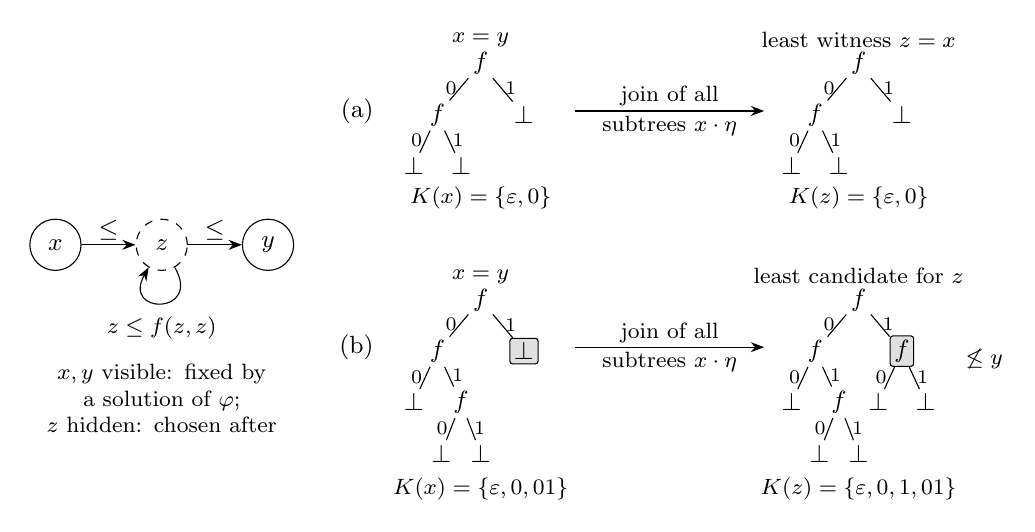
\begin{tikzpicture}[>=Stealth,font=\small,
    every node/.style={inner sep=1.5pt},
    var/.style={draw,circle,minimum size=6.5mm,inner sep=0pt},
    hid/.style={var,dashed},
    tree/.style={level distance=6.5mm,
      level 1/.style={sibling distance=11mm},
      level 2/.style={sibling distance=6mm},
      level 3/.style={sibling distance=5mm}},
    hl/.style={draw,rounded corners=1pt,fill=black!12},
    lb/.style={font=\footnotesize,align=center},
    e0/.style={left,font=\scriptsize,inner sep=1pt,pos=0.45},
    e1/.style={right,font=\scriptsize,inner sep=1pt,pos=0.45}]
  % the consequent: visible x, y and hidden z
  \node[var] (x) at (0,0.2) {$x$};
  \node[hid] (z) at (1.35,0.2) {$z$};
  \node[var] (y) at (2.7,0.2) {$y$};
  \draw[->] (x) -- node[above]{$\le$} (z);
  \draw[->] (z) -- node[above]{$\le$} (y);
  \path (z) edge[->,loop below,min distance=7mm,in=-120,out=-60] (z);
  \node[lb] at (1.35,-0.85) {$z\le f(z,z)$};
  \node[lb,text width=3.3cm] at (1.35,-1.75)
    {$x,y$ visible: fixed by\\ a solution of $\varphi$;\\
     $z$ hidden: chosen after};
  % row (a)
  \node[anchor=east,font=\small] at (4.1,1.9) {(a)};
  \begin{scope}[tree]
    \node (a1) at (5.4,2.5) {$f$}
      child {node {$f$} child {node {$\Bot$} edge from parent node[e0]{0}}
                        child {node {$\Bot$} edge from parent node[e1]{1}}
             edge from parent node[e0]{0}}
      child {node {$\Bot$} edge from parent node[e1]{1}};
    \node (a2) at (10.2,2.5) {$f$}
      child {node {$f$} child {node {$\Bot$} edge from parent node[e0]{0}}
                        child {node {$\Bot$} edge from parent node[e1]{1}}
             edge from parent node[e0]{0}}
      child {node {$\Bot$} edge from parent node[e1]{1}};
  \end{scope}
  \node[lb,anchor=south] at (5.4,2.65) {$x=y$};
  \node[lb,anchor=south] at (10.2,2.65) {least witness $z=x$};
  \node[lb] at (5.4,0.8) {$\Kpos(x)=\{\eps,0\}$};
  \node[lb] at (10.2,0.8) {$\Kpos(z)=\{\eps,0\}$};
  \draw[->] (6.6,1.9) -- node[above,lb]{join of all} node[below,lb]{subtrees $x\cdot\eta$} (9.0,1.9);
  % row (b)
  \node[anchor=east,font=\small] at (4.1,-1.1) {(b)};
  \begin{scope}[tree]
    \node (b1) at (5.4,-0.5) {$f$}
      child {node {$f$} child {node {$\Bot$} edge from parent node[e0]{0}}
                        child {node {$f$} child {node {$\Bot$} edge from parent node[e0]{0}}
                                          child {node {$\Bot$} edge from parent node[e1]{1}}
                               edge from parent node[e1]{1}}
             edge from parent node[e0]{0}}
      child {node[hl] (b1r) {$\Bot$} edge from parent node[e1]{1}};
    \node (b2) at (10.2,-0.5) {$f$}
      child {node {$f$} child {node {$\Bot$} edge from parent node[e0]{0}}
                        child {node {$f$} child {node {$\Bot$} edge from parent node[e0]{0}}
                                          child {node {$\Bot$} edge from parent node[e1]{1}}
                               edge from parent node[e1]{1}}
             edge from parent node[e0]{0}}
      child {node[hl] (b2r) {$f$} child {node {$\Bot$} edge from parent node[e0]{0}}
                                  child {node {$\Bot$} edge from parent node[e1]{1}}
             edge from parent node[e1]{1}};
  \end{scope}
  \node[lb,anchor=south] at (5.4,-0.35) {$x=y$};
  \node[lb,anchor=south] at (10.2,-0.35) {least candidate for $z$};
  \node[lb] at (5.4,-2.9) {$\Kpos(x)=\{\eps,0,01\}$};
  \node[lb] at (10.2,-2.9) {$\Kpos(z)=\{\eps,0,1,01\}$};
  \draw[->] (6.6,-1.1) -- node[above,lb]{join of all} node[below,lb]{subtrees $x\cdot\eta$} (9.0,-1.1);
  \node[lb,anchor=west] at (11.5,-1.25) {$\not\le y$};
\end{tikzpicture}
\caption{The shift closure of \cref{ex:intro-shift} over $\BF$. A solution of
$\varphi$ fixes the visible variables $x$ and $y$; the hidden $z$ is chosen
afterwards and depends on it. The literal $z\le f(z,z)$ makes the
constructor positions of $z$ closed under suffixes, so $z$ must lie above every
subtree of $x$, and their join is the least candidate. (a) For
$x=y=f(f(\Bot,\Bot),\Bot)$ the candidate is $x$ itself, which fits below $y$.
(b) For $x=y=f(f(\Bot,f(\Bot,\Bot)),\Bot)$, the countermodel of $\varphi_1$, the
position $01$ of $x$ forces a constructor of $z$ at its suffix $1$ (shaded),
where $y$ has the leaf $\Bot$; no $z$ exists.}
\Description{On the left, three circles x, z and y joined by arrows labeled
less or equal, with a loop at z for z below f of z and z; the circle of z is
dashed because z is hidden. On the right, two rows. In row a, the tree
f of f of bottom and bottom, and bottom, which is both x and y, is joined by an arrow
labeled join of all subtrees to the same tree, the least witness for z. In
row b, the tree of x and y has constructor positions epsilon, 0 and 01, and
the arrow leads to a tree with an extra constructor at position 1, shaded
together with the leaf bottom of y at position 1; the least candidate for z is not below
y.}
\label{fig:intro-shift}
\end{figure}


\paragraph{An Open Problem}
In non-structural subtyping, $\Bot\le t\le\Top$ relates trees of different
shapes. Plain non-structural subtype entailment was posed as an open problem
in 1996 \citep{Rehof96TLCA}, and \citet{Zhao26} decides it for one
constructor of any arity and variance. The existential
problem has been open since the same year. \citet[Section~1]{TrifonovSmith96}
``leave open the question whether it is decidable'' and decide a sound
approximation. \citet[Section~3.2]{FahndrichAiken96} write that ``no complete
algorithm is known''. \citet[Section~7.2.2]{Su02} writes that ``for
existential entailment and subtyping constrained types, virtually nothing is
known at this point, except the lower bounds carried over from entailment'',
and that for non-structural subtyping the problem ``may in fact be
undecidable'', because an alternative undecidability proof for the
first-order theory appears to use a single quantifier alternation.
\citet[Section~1.4.2]{Priesnitz04} calls subtyping of constrained types a
``prominent open problem''. The first-order theory is indeed undecidable,
already over $\BF$ with $f$ binary and covariant, in all three tree classes
\citep{SuAikenNiehrenPriesnitzTreinen02}, but with six quantifier blocks and a
matrix with disjunctions and negations, whereas existential entailment has one
alternation, and its antecedent and consequent are conjunctions. Over feature
trees, existential entailment is decided by an inclusion of finite automata
\citep{MullerNiehrenTreinen98,MullerNiehrenTreinen01}, in a setting where a
fresh feature is always available, which a constructor of fixed arity does not
offer (\cref{sec:rel}).

\paragraph{Our Result}
We fix one constructor $f$ of arity $n\ge0$ and a \emph{variance}
$c:\{0,\ldots,n-1\}\to\{0,1\}$, which makes each argument covariant or
contravariant; the arrow is $n=2$ with $c(0)=1$ and $c(1)=0$
(\cref{sec:bg-trees}). Trees may be infinite unless stated otherwise.

\begin{theorem}[Main theorem]\label{thm:intro-main}
For every arity $n\ge0$ and every variance $c$, existential entailment
$\varphi\entails\Exists\psi$ over $\BFT$ is decidable over arbitrary, over
regular, and over finite trees. Over $\BF$, the same holds when $f$ is
covariant. If $\varphi$ and $\psi$ are satisfiable in the tree class considered
and the entailment fails, then the failure is certified by a
\emph{counterexample word} of length at most $E_3(O(s))$: a word over the
argument positions of $f$, or two such words joined by a separator, from which
a countermodel is computed (\cref{def:as-certificate}). Here
$E_3(x)=2^{2^{2^x}}$, $s$ is the number of variables after flattening, every
introduced name and every hidden variable included, and the constant does not
depend on $n$.
\end{theorem}

\Cref{sec:as} defines counterexample words (\cref{def:as-certificate}),
states the theorem precisely (\cref{thm:as-main}), shows that every
counterexample word yields a countermodel effectively
(\cref{lem:as-countermodel}), and assembles the proof. The theorem needs no restriction on the polarity of
the variables: a variable may occur both co- and contravariantly, in the
antecedent and in the consequent. In particular, it decides the subsumption of
\citet{TrifonovSmith96} between constrained types over $\Bot$, $\to$ and
$\Top$, and the correctness of simplifications of such types
(\cref{sec:ap}). We do not claim the signature $\BF$ with a contravariant
argument; \cref{rem:tc-gadget-needed} explains why the reduction to $\BFT$
needs covariance.

\paragraph{Bounds and Complexity}
\Cref{prop:as-bounds} and \cref{sec:cx} refine the theorem. Only two kinds of
failure, both described in \cref{sec:intro-overview}, have triply exponential
bounds: failures of condition \CondU\ and \emph{mortal holes}. The larger
bound belongs to the mortal holes, the only case that needs a new compression
technique; all other failures have singly exponential witnesses. The decision procedure does not enumerate words: a
nondeterministic search builds a witness level by level, keeping only a
summary of each level, and runs in 2-EXPSPACE, hence in 3-EXPTIME
(\cref{prop:cx-search,thm:cx-upper}); for plain entailment this saves one
exponential in space over the procedure of \citet{Zhao26} (\cref{rem:cx-plain}). For a unary
constructor, $n=1$, witnesses are singly exponential and the problem is in
PSPACE, for both variances and all three tree classes (\cref{thm:cx-unary}),
and for $n=0$ it is a finite enumeration (\cref{rem:cx-nullary}). On the
other side, shortest counterexample words can have length $2^{\Omega(s)}$
(\cref{prop:cx-length}), and the problem is PSPACE-hard for every fixed arity
$n\ge2$, already with $f$ covariant, by explicit reductions that use the additional arguments of $f$; bare
padding of a binary construction does not suffice (\cref{thm:cx-hard} and
\cref{ex:cx-padding}). The gap between PSPACE and 2-EXPSPACE, the gap between
singly and triply exponential witnesses, and hardness for $n=1$ remain open.

\paragraph{Mechanization}
The decidability results are checked in the Lean~4 proof assistant
\citep{MouraUllrich21} with Mathlib \citep{Mathlib20}: over $\BFT$ for every
arity, arity zero included, every variance and all three tree classes, and
over $\BF$ with $f$ covariant (\cref{sec:mechanization}). Each of the six
procedures is a computable definition with a correctness theorem without
premises, and plain entailment is decided as the special case without hidden
variables. The anchored compression of \cref{sec:mo} is mechanized with an
elementary bound of the same form as ours, and all search bounds are explicit
functions of the numbers of automaton states. The procedures take flat
literals as input. The flattening of arbitrary type expressions
(\cref{lem:bg-flattening}), the bounds in terms of the number of variables, the
construction of countermodels and the complexity results are not mechanized.

\subsection{Overview of the Proof}\label{sec:intro-overview}

The proof follows a single route for all arities and variances
(\cref{fig:intro-overview}). It works over $\BFT$ and arbitrary trees and
transfers the result to the other tree classes and to $\BF$ at the end. We end
in the hole problem of the plain-entailment proof~\citep{Zhao26}, whose readers, holes and bounds
\cref{sec:bg} recalls: a \emph{reader} is a deterministic automaton with
rejected states and an admission relation on pairs of states; a
\emph{comparison} of a word $w$ is a pair of cuts $(s,e)$, $s<e$, such that the
suffix after $e$ is a prefix of the suffix after $s$; and a \emph{hole} is a
rejected word without an admitted comparison. That proof bounds a
shortest hole in three steps: a short rejected tail, a bound on the
\emph{depth}, a measure of nested repetition, and a compression of words of
bounded depth. What is new here is that some of our holes must also
\emph{contain} a comparison of a particular kind, and that a single word may
be dead because of a comparison with itself.

\begin{figure}[tbp]
\centering
\small
\hyphenpenalty=10000\relax
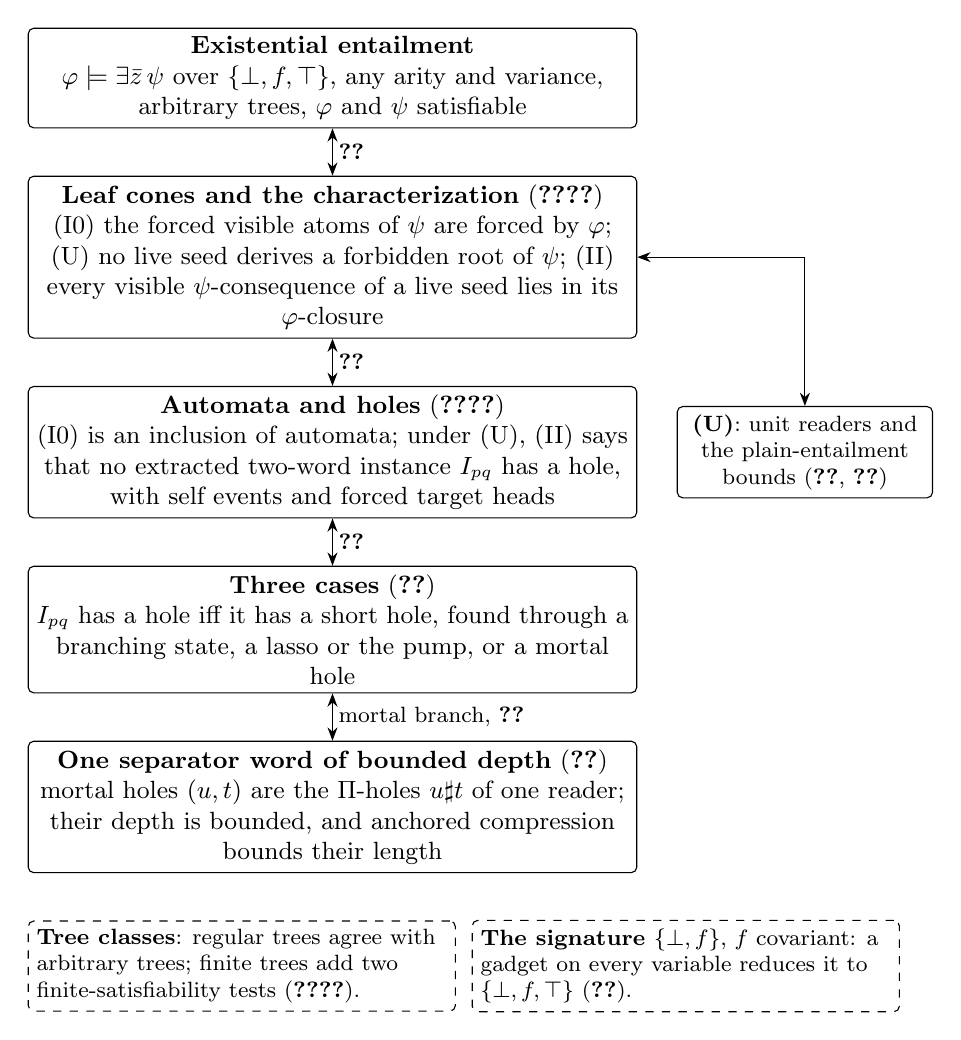
\begin{tikzpicture}[
    node distance=6mm,
    >=Stealth,
    stepbox/.style={draw, rounded corners=2pt, align=flush center,
                 text width=0.62\linewidth, inner sep=3pt, font=\small},
    ubox/.style={draw, rounded corners=2pt, align=flush center,
                 text width=0.25\linewidth, inner sep=3pt, font=\footnotesize},
    sidebox/.style={draw, dashed, rounded corners=2pt, align=flush left,
                 text width=0.43\linewidth, inner sep=3pt, font=\footnotesize},
    thm/.style={right, font=\footnotesize, inner sep=2pt}]
  \node[stepbox] (ent)
    {\textbf{Existential entailment}\\
     $\varphi\entails\Exists\psi$ over $\BFT$, any arity and variance, arbitrary
     trees, $\varphi$ and $\psi$ satisfiable};
  \node[stepbox, below=of ent] (ch)
    {\textbf{Leaf cones and the characterization}
     (\cref{sec:lf,sec:ch})\\
     \CondI\ the forced visible atoms of $\psi$ are forced by $\varphi$;
     \CondU\ no live seed derives a forbidden root of $\psi$;
     \CondII\ every visible $\psi$-consequence of a live seed lies in its
     $\varphi$-closure};
  \node[stepbox, below=of ch] (ex)
    {\textbf{Automata and holes} (\cref{sec:sm,sec:ex})\\
     \CondI\ is an inclusion of automata; under \CondU, \CondII\ says that no
     extracted two-word instance $I_{pq}$ has a hole, with self events and
     forced target heads};
  \node[stepbox, below=of ex] (nm)
    {\textbf{Three cases} (\cref{sec:nm})\\
     $I_{pq}$ has a hole iff it has a short hole, found through a branching
     state, a lasso or the pump, or a mortal hole};
  \node[stepbox, below=of nm] (mo)
    {\textbf{One separator word of bounded depth} (\cref{sec:mo})\\
     mortal holes $(u,t)$ are the $\Pi$-holes $u\sep t$ of one reader; their
     depth is bounded, and anchored compression bounds their length};
  \node[ubox, right=5mm of ex] (u)
    {\textbf{\CondU}: unit readers and the plain-entailment bounds
     (\cref{sec:un}, \cref{thm:un-decidable})};
  \draw[<->] (ent) -- node[thm]{\cref{thm:ch-characterization}} (ch);
  \draw[<->] (ch) -- node[thm]{\cref{thm:ex-reduction}} (ex);
  \draw[<->] (ex) -- node[thm]{\cref{thm:nm-three-cases}} (nm);
  \draw[<->] (nm) -- node[thm, align=left]{mortal branch,
    \cref{thm:mo-decide}} (mo);
  \draw[<->] (ch.east) -| (u.north);
  \node[sidebox, below=6mm of mo.south west, anchor=north west] (cls)
    {\textbf{Tree classes}: regular trees agree with arbitrary trees; finite
     trees add two finite-satisfiability tests
     (\cref{thm:tc-regular,thm:tc-finite}).};
  \node[sidebox, right=2mm of cls] (bf)
    {\textbf{The signature $\BF$}, $f$ covariant: a gadget on every variable
     reduces it to $\BFT$ (\cref{thm:tc-gadget}).};
\end{tikzpicture}
\caption{The route of the proof, for satisfiable $\varphi$ and $\psi$ over
$\BFT$ and arbitrary trees. Each double arrow is an equivalence, labeled with
the result that proves it, or for condition \CondU\ with its box; the last
vertical one concerns only the mortal branch of the case split, whose short
holes are found directly. Condition \CondU\ leaves the
main route: it is a hole problem of the kind solved for plain entailment,
decided by the bounds of \citet{Zhao26}. Here $p,q$ range over the visible signed variables. The
dashed boxes describe the transfers to the other tree classes and to $\BF$.
\Cref{sec:as} assembles the steps.}
\Description{Five boxes connected by double arrows, each labeled with a
theorem, lead from existential entailment to the characterization by three
conditions on leaf cones, to automata and two-word hole problems, to a case
split into short holes and mortal holes, and, for the mortal branch, to holes
of one separator word of bounded depth. A side box, reached from the
characterization, decides condition (U) by unit readers and the
plain-entailment bounds. Two dashed boxes describe the regular and finite tree classes and the
signature without top.}
\label{fig:intro-overview}
\end{figure}

\paragraph{Leaf cones}
Over $\BF$ with $f$ covariant, a tree is its set of constructor positions,
solution sets are closed under unions and intersections, and every literal
becomes a set of implications with one premise (\cref{rem:ch-one-sign}).
With $\Top$ and variance, a literal can relate a leaf $\Top$ of one tree to a
leaf $\Bot$ of another, and one set of positions no longer describes a tree.
We restore a Horn structure for every arity and variance by describing a tree
$t$ through
its two \emph{leaf cones}: the words whose path meets a leaf of $t$ of
\emph{sign}~$0$, and those whose path meets a leaf of sign~$1$, where the sign
of a leaf combines its label, $\Top$ or $\Bot$, with the polarity of its path.
The two cones are disjoint and closed under extension, every such pair of sets
is the pair of exactly one tree, and the order of variance $c$ adds leaves of
sign~$0$ and removes leaves of sign~$1$ (\cref{thm:lf-representation}). An
\emph{atom} $(v^\pm,w)$ says that $w$ lies in a cone of $v$. Every literal
becomes \emph{pure moves}, implications between atoms that copy, push or pop
the first letter of the word as on a stack, together with \emph{facts}, atoms
that every solution contains, and \emph{forbidden roots}, atoms that none
contains (\cref{lem:lf-clauses}). The only all-negative binary clauses are the
exclusions of opposite atoms, which are the same for every system. So least models are
closures of seeds, every atom of a closure has a single seed
(\cref{lem:lf-closure}), every pure move has a dual of opposite sign
(\cref{lem:lf-duality}), and two derivations that collide in an exclusion can
be merged into one (\cref{lem:lf-collision}).

\paragraph{Three conditions}
Collision return turns every obstruction to extending a solution of $\varphi$
into an obstruction at a single seed. If both systems are satisfiable,
$\varphi\entails\Exists\psi$ holds iff three conditions hold
(\cref{thm:ch-characterization}): \CondI, every visible atom that $\psi$
forces is forced by $\varphi$; \CondU, $\psi$ derives no forbidden root from a
visible atom that some solution of $\varphi$ contains; and \CondII, every
visible atom that $\psi$ derives from such an atom lies in the least solution
of $\varphi$ that contains it.

\paragraph{Pushdown summaries}
The pure moves form a pushdown system whose control states are the signed
variables. Two deterministic automata summarize it: after reading a word
$\gamma$, the \emph{upper automaton} of $p$ holds the signed variables reached
from $p$ by popping $\gamma$, and after reading $\beta$ the \emph{lower
automaton} of $q$ holds those from which $q$ is reached by pushing $\beta$.
Every pure derivation splits at its lowest point into a \emph{pop head}, read
by the first, and a \emph{push head}, read by the second, above a common
suffix (\cref{lem:sm-lowest-point}). Variance adds a new reason for an atom to
be dead. Besides a reachable forbidden root, or an opposite extension forced
by the facts, which make an atom \emph{dead by support}, the closure of a seed
$(p,w)$ may contain the opposite of an extension of the seed. For a seed that is not already dead
by support, this happens exactly when two cuts of the single word $w$ form a
comparison whose automaton states are related: a \emph{self event} (\cref{thm:sm-dead}). Self events occur only
through contravariant directions (\cref{rem:sm-parity}), and the set of live
words need not be regular (\cref{ex:sm-arrow}). Condition \CondI\ is an
inclusion of automata, decidable in polynomial space (\cref{prop:sm-decide}).

\paragraph{Condition (U) as a hole problem}
A failure of \CondU\ is a word $w$ such that $(p,w)$ is live in $\varphi$ and
leads to a forbidden root in $\psi$. Liveness is the absence of deadness by
support, a regular property, and of self events, which are comparisons of $w$.
So the failures are exactly the holes of a single reader, the \emph{unit
reader}, whose admitted comparisons are the self events
(\cref{lem:un-holes}). It has the rejected-path property of \citet{Zhao26}, and
the bounds proved there decide \CondU\ (\cref{thm:un-decidable}). A smaller reader
with the same holes, together with a clock that reads only the antecedent and
bounds the depth, keeps the length bound for \CondU\ below the one for mortal
holes.

\paragraph{Two-word holes with self events}
A failure of \CondII\ consists of a live seed $(p,t)$, a pure derivation of
$\psi$ from it to a visible atom $(q,u)$, and the fact that $(q,u)$ lies
outside the closure of the seed in $\varphi$. Each part is read by automata on
the two words: the derivation is a \emph{head event}, a pair of cuts at which
$t$ and $u$ have equal suffixes; membership in the closure is an \emph{event},
a pair of cuts $(s,e)$ at which the suffix of $t$ after $e$ is a prefix of the
suffix of $u$ after $s$; and liveness of the seed forbids self events of $t$.
So, once \CondU\ holds, \CondII\ fails iff an \emph{extracted instance}
$I_{pq}$ of a hole problem for two words has a \emph{hole}: a safe spine $u$,
a rejected target $t$, a head event, and neither an event nor a self event
(\cref{def:ex-ss2self,thm:ex-reduction}). The target automaton marks a cut of
the seed as rejected only while the seed is still a candidate, neither dead by
support in $\varphi$ nor root-dead in $\psi$. Under \CondU\ this enriched
rejection loses nothing, and it forces every pop head of $\psi$ to end before
the first rejected cut, condition (FH) (\cref{lem:ex-fh}).

\paragraph{Holes that are not mortal}
Cut a hole $(u,t)$ at the first rejected cut of its target. By (FH) the rest
$\theta$ of the target is a common suffix of both words, and what remains is a
\emph{pre-hole}. Appending $\theta$ to a pre-hole creates no new event and no
new self event, and it keeps an old one exactly when $\theta$ continues its
\emph{overhang}, the part of one suffix that the other does not cover,
periodically (\cref{lem:nm-continuation}). So the question is whether one safe
continuation breaks every such periodicity obligation. If the spine ends
in a \emph{branching} state, which reaches a cycle with a choice of letters, a
breaking continuation exists by the theorem of \citet{FineWilf65}
(\cref{lem:nm-breaker}). If it ends in a \emph{thin} state, long safe
continuations follow finitely many lassos; a lasso that is not purely periodic
breaks everything, and for a purely periodic lasso the \emph{pump} shortens
the pre-hole itself, keeping the obligations broken (\cref{thm:nm-pump}).
Short pre-holes are found by a finite graph (\cref{prop:nm-short-prehole}). In
the remaining case the hole is \emph{mortal}: its spine ends in a state
without an infinite safe continuation, and its target ends shortly after its
first rejected cut (\cref{thm:nm-three-cases}). Outside the mortal case,
holes are polynomial in the sizes of the automata, hence singly exponential
in~$s$.

\paragraph{Mortal holes}
In a mortal hole the continuation is short, but the common suffix of the two
words can be long, so the pair itself must be shortened, with both words
together. We pack them into one word $u\sep t$ around a separator. Events and
self events become comparisons of this word, and a head event becomes an
\emph{anchored} comparison, one whose matched factor is followed by the
separator (\cref{lem:mo-sep}). Mortal holes are exactly the
\emph{$\Pi$-holes} of one reader, its holes with an anchored comparison whose
state pair lies in a relation $\Pi$ (\cref{lem:mo-pi-reader}), and the short
rejected tail bounds their depth by the depth theorem of \citet{Zhao26}
(\cref{lem:mo-depth}). The bounded-depth compression of that paper keeps every negative
condition but can delete the letters on which the anchored comparison depends
(\cref{ex:mo-loses}). A \emph{positive channel} records the anchored witness
at each level of the hierarchy (\cref{lem:mo-desub}). The channel is added to
the information that this compression compares before it merges
letters or deletes columns, so every shortening keeps some anchored witness.
This gives the anchored compression theorem (\cref{thm:mo-anchored}) and a
triply exponential bound on mortal holes (\cref{cor:mo-extracted}), the
largest of our bounds, which decides the two-word problem under (FH)
(\cref{thm:mo-decide}).

\paragraph{Tree classes and the signature without top}
Over regular trees the closure of regular seeds is regular, and a failure has
at most two seeds, so regular and arbitrary trees give the same answer
(\cref{thm:tc-regular}). Least models are infinite in general, so finite trees
need a different argument: the at most two observations behind a failure are
expressed by finite ground bounds, and adding finite ground bounds preserves
finite satisfiability, for every variance (\cref{thm:tc-pinning}). This gives
the dispatch of \cref{thm:tc-finite}. For $\BF$ with $f$ covariant, the
literals $v\le y_v$ and $y_v\le f(y_v,\ldots,y_v)$ force $v$ to be free of
$\Top$, and placing them on every visible and every hidden variable reduces
$\BF$ to $\BFT$ in each tree class (\cref{thm:tc-gadget}).

\paragraph{The running examples}
Two examples recur through the paper (\cref{tab:intro-examples}). The first is
the shift closure of \cref{ex:intro-shift}, for a covariant constructor; the
second follows the antecedent $x\le x\to x$ for the arrow, in which $x$ occurs
at both polarities. For a covariant constructor, and more generally on
instances with a joint parity assignment, self events do not occur and every
dead atom is dead by support
(\cref{rem:ch-parity,rem:sm-parity,rem:ex-covariant}); over $\BF$ the three
conditions compare unions of solutions, least solutions, and closures of
single positions (\cref{rem:ch-one-sign}).

\begin{table}[tbp]
\caption{The running examples.}
\label{tab:intro-examples}
\centering
\small
\begin{tabular}{@{}>{\raggedright\arraybackslash}p{0.21\linewidth}>{\raggedright\arraybackslash}p{0.17\linewidth}>{\raggedright\arraybackslash}p{0.54\linewidth}@{}}
\toprule
Example & Sections & What it shows\\
\midrule
\multicolumn{3}{@{}l}{\emph{Shift closure}: $\psi=x\le z\wedge z\le y\wedge
  z\le f(z,z)$, with $f$ binary and covariant}\\
\cref{ex:intro-shift} & \cref{sec:intro} & an existential entailment that is
  an infinite family of plain entailments\\
\cref{ex:sm-running} & \cref{sec:sm} & the signed system over $\BFT$ and its
  pure derivations\\
\cref{ex:un-running} & \cref{sec:un} & \CondU\ fails at $x=y=\Top$, and holds
  once $y$ is restricted to trees without $\Top$\\
\cref{ex:ex-running} & \cref{sec:ex} & \CondII\ fails by the hole $(01,1)$ of
  an extracted instance, whose spine ends in a branching state\\
\cref{ex:nm-running} & \cref{sec:nm} & the pre-hole $(0,\eps)$, its single
  obligation, and, after \cref{lem:nm-breaker}, a breaker\\
\cref{ex:as-running} & \cref{sec:as} & the procedure end to end: the hole word
  $01\sep1$, its two pins, and the finite countermodel of
  \cref{ex:intro-shift}\\
\midrule
\multicolumn{3}{@{}l}{\emph{The arrow}: the antecedent $x\le x\to x$}\\
\cref{ex:lf-clauses,ex:lf-least} & \cref{sec:lf} & a single-seed
  inconsistency\\
\cref{ex:ch-arrow} & \cref{sec:ch} & the entailment
  $x\le x\to x\entails\exists z\,(x\le z\to z)$, whose failure without the
  antecedent needs collision return\\
\cref{ex:sm-arrow} & \cref{sec:sm} & a nonregular set of dead words\\
\cref{ex:un-arrow,ex:ex-arrow} & \cref{sec:un,sec:ex} & why admitted self
  events and the enrichment of the target automaton are needed\\
\bottomrule
\end{tabular}
\end{table}

\paragraph{Contributions}
\begin{itemize}[leftmargin=*]
\item \emph{Decidability} (\cref{thm:intro-main}). Existential entailment is
  decidable for one constructor of every arity and every variance over
  $\BFT$, and over $\BF$ with $f$ covariant, in all three tree classes. This
  settles the decidability question of \citet{TrifonovSmith96} for semantic
  subsumption of constrained types.
\item \emph{Signed leaf cones} (\cref{sec:lf,sec:ch}). A representation of
  trees of any variance in which every system is a Horn system with unary
  rules, and a characterization of existential entailment by three conditions
  on single seeds.
\item \emph{Self events} (\cref{sec:sm,sec:un,sec:ex}). Deadness is deadness by
  support or a self event, a comparison of one word with itself. Both
  \CondU\ and \CondII\ become hole problems whose admissions include self
  events, the second with an enriched rejection that makes target heads forced.
\item \emph{Non-mortal holes} (\cref{sec:nm}). Breakers, lassos and a pump
  with polynomial capacity give singly exponential witnesses outside the
  mortal case.
\item \emph{Anchored compression} (\cref{sec:mo}). Positive channels extend the
  bounded-depth compression of \citet{Zhao26} to holes that must contain
  an anchored comparison.
\item \emph{Tree classes and $\BF$} (\cref{sec:tc}). Regular and finite
  transfers for every variance, and a reduction of covariant $\BF$ to $\BFT$.
\item \emph{Complexity} (\cref{sec:cx}). Elementary witness bounds; a
  2-EXPSPACE decision by summary search; PSPACE for $n\le1$; exponential
  shortest witnesses; and PSPACE-hardness for every fixed arity $n\ge2$,
  already with $f$ covariant.
\item \emph{Applications} (\cref{sec:ap}). Subsumption of constrained type
  schemes and correctness of simplification are decidable, including arrow
  types without any restriction on polarity, and several classes reduce
  directly to plain entailment.
\item \emph{Mechanization} (\cref{sec:mechanization}). Computable decision
  procedures for all six cases of \cref{thm:intro-main}, checked in Lean~4,
  including anchored compression with an elementary bound.
\end{itemize}

\paragraph{Organization}
\Cref{sec:bg} fixes notation and recalls the results of \citet{Zhao26} that we use.
\Cref{sec:lf,sec:ch,sec:sm,sec:un,sec:ex,sec:nm,sec:mo,sec:tc} follow the
route above, and \cref{sec:as} assembles the proof.
\Cref{sec:ap,sec:cx,sec:mechanization,sec:rel,sec:concl} discuss
applications, complexity, the mechanization, related work, and open problems. Omitted proofs are in the appendices.
\Cref{sec:lf,sec:ch} give the characterization, and
\cref{sec:sm,sec:un,sec:ex} turn it into hole problems; \cref{sec:nm,sec:mo} are the technical core, and
\cref{sec:mo} assumes \cref{sec:bg-hierarchy}. A reader interested in the
result and its use may go from \cref{sec:ch} to \cref{sec:as,sec:ap}.

%% background — words; trees of arity n with variance c, normalization and
%% duality, tree classes; flat systems, signed systems, existential entailment,
%% flattening; the results of Zhao26 on constraints; readers, holes, the
%% rejected-path property, the canonical hierarchy, the tail, depth and search
%% theorems of Zhao26, lettered monitors, derivatives and the label facts, and
%% an outline of the search. Further results of Zhao26 are in app:bg.

\section{Background}\label{sec:bg}

Throughout the paper we fix an arity $n\ge0$ and a variance $c$ of the
constructor $f$. This section fixes the notation for words, trees, and
constraints, defines existential entailment, and states the results that we
use from the decidability proof for plain entailment of \citet{Zhao26}. That
paper treats one constructor of every arity and every variance; we cite its
results in that generality. Short proofs are repeated; all other cited results
are stated exactly and proved there. \Cref{app:bg} collects the further
results of that paper used later: the satisfiability criteria, the cores lemma, the ordinary
and symbolic states of derived monitors, the structure of the bounded-depth
search, and its constants.

\subsection{Words}\label{sec:bg-words}
Put $\Sigma=\{0,\ldots,n-1\}$, the alphabet of \emph{directions}; the letter
$i$ names the $i$th argument of $f$. For $n=0$ the alphabet is empty and $\eps$
is the only word over it. Readers (\cref{sec:bg-readers}) also work over other
finite alphabets, written $\Gamma$, for instance $\Sigma\sqcup\{\sep\}$.

Words are finite unless they are explicitly called infinite. For a word $w$, a
\emph{cut} is an integer $j$ with $0\le j\le\len w$; it separates the first $j$
letters from the rest. We write $w[i]$ for the letter at position $i$, where
$0\le i<\len w$, and $\wpre wj$, $\wsub wjh$, and $\wsuf wj$ for the prefix,
factor, and suffix at the indicated cuts. The empty word is $\eps$, and
$u\pre w$ means that $u$ is a prefix of $w$. For a set $L$ of words and a word
$\beta$, put $\beta L=\{\beta\sigma:\sigma\in L\}$ and
$\beta^{-1}L=\{\sigma:\beta\sigma\in L\}$. A positive integer $\varpi$ is a
\emph{period} of $w$ if $w[i]=w[i-\varpi]$ for $\varpi\le i<\len w$. For a
nonempty word $o$, we write $\theta\pre o^\omega$ if $\theta\pre o^k$ for some
$k\ge0$.

\begin{lemma}[Periodic prefixes {\nssecite{Lemma ``Periodic prefixes''}}]\label{lem:bg-periodic}
For every nonempty word $o$ and every word $\theta$, $\theta\pre o\theta$ iff
$\theta\pre o^\omega$.
\end{lemma}
\begin{proof}
If $\theta\pre o^k$, then $o\theta\pre o^{k+1}$ and $\theta\pre o^{k+1}$; of
two prefixes of one word the shorter is a prefix of the longer, so
$\theta\pre o\theta$. Conversely, let $\theta\pre o\theta$. If
$\len\theta\le\len o$, then $\theta\pre o$. Otherwise $\theta=o\theta'$ for a
word $\theta'$, and $o\theta'\pre oo\theta'$ gives $\theta'\pre o\theta'$. By
induction on the length, $\theta'\pre o^k$ for some $k$, so
$\theta\pre o^{k+1}$.
\end{proof}

\subsection{Trees, Variance, and Normalization}\label{sec:bg-trees}

\paragraph{Trees}
Order the labels by $\Bot<f<\Top$. A \emph{tree} is a partial map
$t:\Sigma^*\rightharpoonup\BFT$ whose domain $\operatorname{dom}(t)$ contains
$\eps$, is prefix closed, and satisfies, for every $w\in\operatorname{dom}(t)$
and every $i\in\Sigma$,
\[
 wi\in\operatorname{dom}(t)\quad\Longleftrightarrow\quad t(w)=f .
\]
The elements of $\operatorname{dom}(t)$ are the \emph{positions} of $t$. We
write $f(t_0,\ldots,t_{n-1})$, or $f(t_i)_i$, for the tree with root label $f$
and subtrees $t_i$ at the positions $i$. The \emph{subtree} of $t$ at a
position $\beta$ is the tree $\beta^{-1}t:w\mapsto t(\beta w)$. The full
constructor tree $\Omega=f(\Omega,\ldots,\Omega)$ has label $f$ at every word;
it is infinite for $n\ge1$, and $\Omega=f()$ for $n=0$. At arity zero the only
trees are $\Bot$, $f()$, and $\Top$.

\paragraph{Variance and the order}
A \emph{variance} is a map $c:\Sigma\to\{0,1\}$; argument $i$ is
\emph{covariant} if $c(i)=0$ and \emph{contravariant} if $c(i)=1$, and $f$ is
covariant if $c=0$. For the arrow, $n=2$, $f(a_0,a_1)=a_0\to a_1$, $c(0)=1$, and
$c(1)=0$. The \emph{polarity} of a word counts its contravariant letters modulo
two:
\begin{equation}\label{eq:bg-polarity}
 \parity(w)=\bigoplus_{j<\len w}c(w[j]),\qquad \parity(\eps)=0,\qquad
 \parity(uv)=\parity(u)\oplus\parity(v).
\end{equation}
The \emph{non-structural order} of variance $c$ is
\begin{equation}\label{eq:bg-order}
 t\le_c u\quad\Longleftrightarrow\quad
 \forall w\in\operatorname{dom}(t)\cap\operatorname{dom}(u)\quad
 \begin{cases}t(w)\le u(w),&\parity(w)=0,\\ u(w)\le t(w),&\parity(w)=1.\end{cases}
\end{equation}
For the covariant variance $c=0$ we write $\le$ and call the order
\emph{covariant}. The relation $\le_c$ is a partial order, and it is the
greatest relation $R$ such that $R(t,u)$ implies $t=\Bot$, or $u=\Top$, or
$t=f(a_i)_i$ and $u=f(b_i)_i$ with $R(a_i,b_i)$ for every $i$ with $c(i)=0$ and
$R(b_i,a_i)$ for every $i$ with $c(i)=1$
\nssecite{Sect.\ ``Non-Structural Subtyping''}. In particular,
$\Bot\le_c t\le_c\Top$ for every tree $t$, and
$f(a_i)_i\le_c f(b_i)_i$ iff each pair of arguments is related in the direction
given by its variance. For the arrow this is the usual rule:
$a_0\to a_1\le_c b_0\to b_1$ iff $b_0\le_c a_0$ and $a_1\le_c b_1$.

\paragraph{Duality and normalization}
The \emph{dual} $t^{\partial}$ of a tree $t$ has the domain of $t$ and the labels of
$t$ with $\Bot$ and $\Top$ exchanged; labels $f$ are unchanged. For a
\emph{sign} $s\in\{0,1\}$, the \emph{normalization} $\nu_s t$ has the domain of
$t$; its label at a position $w$ is that of $t$ with $\Bot$ and $\Top$ exchanged
if $s\oplus\parity(w)=1$, and unchanged otherwise. Thus $\nu_0$ exchanges the
extreme labels at the positions of odd polarity and $\nu_1$ at those of even
polarity. The polarity is taken at actual positions of $t$ only; a leaf is
never followed by further letters. For covariant $f$, $\nu_0t=t$ and
$\nu_1t=t^{\partial}$. We also write $+$ for the sign $0$ and $-$ for the sign $1$.

\begin{lemma}[Normalization {\nssecite{Lemma ``Normalization''}}]\label{lem:bg-normalization}
For every variance $c$, all trees $t,u,t_0,\ldots,t_{n-1}$, and every sign $s$:
\begin{enumerate}[leftmargin=*]
\item $\nu_s f(t_i)_i=f(\nu_{s\oplus c(i)}t_i)_i$,\quad
  $\nu_1t=(\nu_0t)^{\partial}=\nu_0(t^{\partial})$,\quad and\quad $\nu_s\nu_st=t$;
\item $t\le_c u$ iff $\nu_0t\le\nu_0u$ iff $\nu_1u\le\nu_1t$;
\item for the covariant order, $t\le u$ iff $u^{\partial}\le t^{\partial}$;
\item the subtree of $\nu_st$ at a position $w$ is $\nu_{s\oplus\parity(w)}(w^{-1}t)$,
  and $\nu_s$ and duality preserve domains, finiteness, and regularity.
\end{enumerate}
\end{lemma}
\begin{proof}
(1) The root of $f(t_i)_i$ is labeled $f$ and is never changed. At a position
$iw$ we have $\parity(iw)=c(i)\oplus\parity(w)$, so the condition $s\oplus\parity(iw)=1$
for $\nu_s$ at $iw$ is the condition for $\nu_{s\oplus c(i)}$ at the position $w$
of $t_i$. The conditions of $\nu_0$ and $\nu_1$ at a position are
complementary, so $\nu_1t$ is $\nu_0t$ with every extreme label exchanged, and
exchanging all extreme labels commutes with exchanging some of them. Applying
$\nu_s$ twice exchanges the same labels twice.

(3) Exchanging $\Bot$ and $\Top$ reverses the chain $\Bot<f<\Top$, and $t$ and
$t^{\partial}$ have the same domain, so every comparison in \cref{eq:bg-order},
read covariantly, is reversed.

(2) The trees $t$ and $\nu_0t$ have the same domain. At a common position $w$
with $\parity(w)=0$, $\nu_0$ changes neither label; at one with $\parity(w)=1$ it
applies the order-reversing exchange to both labels, so $u(w)\le t(w)$ iff
$(\nu_0t)(w)\le(\nu_0u)(w)$. Hence \cref{eq:bg-order} for $\le_c$ is the
covariant comparison of $\nu_0t$ and $\nu_0u$ at every common position. The
second equivalence follows from (1) and (3) for the covariant order.

(4) The first assertion follows from (1) by induction on $w$. So the subtrees
of $\nu_st$ are among the trees $\nu_0t'$ and $\nu_1t'$ for subtrees $t'$ of
$t$, which are finitely many if $t$ is regular. Domains are preserved by
definition, and duality is handled in the same way.
\end{proof}

Thus $\nu_0$ is an order isomorphism from the trees ordered by $\le_c$ onto the
trees ordered covariantly, and $\nu_1$ is an order anti-isomorphism. This is
how variance is removed: a constraint of variance $c$ about $t$ becomes a pair
of covariant constraints about $\nu_0t$ and $\nu_1t$
(\cref{lem:bg-signed}).

\paragraph{Tree classes}
We consider three \emph{tree classes}: the class $\Trees$ of all trees,
possibly infinite; the class $\Trees_{\mathrm{reg}}$ of \emph{regular} trees,
which have finitely many distinct subtrees; and the class $\Trees_{\mathrm{fin}}$
of \emph{finite} trees, which have finite domain. Then
$\Trees_{\mathrm{fin}}\subseteq\Trees_{\mathrm{reg}}\subseteq\Trees$, and
$\Omega$ is regular but not finite for $n\ge1$. A tree is regular iff it is the
unfolding of a finite graph whose constructor nodes have $n$ ordered successors
\nssecite{Sect.\ ``Words and Trees''}. Constructor application and the
constants preserve each class. At arity zero the three classes coincide.

\paragraph{Trees over $\BF$}
A \emph{tree over $\BF$} is a tree without the label $\Top$. For a tree class
$\mathcal D$, its trees over $\BF$ form the corresponding class over $\BF$;
constructor application and $\Bot$ preserve it. We use the signature $\BF$ only
with $f$ covariant. Then a tree $t$ over $\BF$ is determined by the set
$\Kpos(t)=\{w:t(w)=f\}$ of its constructor positions, which is prefix closed,
and every prefix-closed set of words is $\Kpos(t)$ for exactly one tree $t$
over $\BF$.

\begin{lemma}[Order over $\BF$]\label{lem:bg-bf-order}
For covariant trees $t,u$ over $\BF$, $t\le u$ iff $\Kpos(t)\subseteq\Kpos(u)$.
\end{lemma}
\begin{proof}
Suppose $\Kpos(t)\subseteq\Kpos(u)$ and let $w$ be a common position. If
$t(w)=f$, then $u(w)=f$; otherwise $t(w)=\Bot$. In both cases
$t(w)\le u(w)$. Conversely, suppose $t\le u$ and $w\in\Kpos(t)$. Every prefix of
$w$ lies in $\Kpos(t)$. By induction on the prefixes $w'$ of $w$, each of them
is a position of $u$, and $f=t(w')\le u(w')$ forces $u(w')=f$, since $u$ has no
label $\Top$. Hence $w\in\Kpos(u)$.
\end{proof}

\subsection{Constraints and Existential Entailment}\label{sec:bg-constraints}

\paragraph{Flat systems}
All variable sets in this paper are finite. Fix such a set. A \emph{flat literal} has one of the forms
\[
 u\le v,\qquad f(a_i)_i\le u,\qquad u\le f(a_i)_i,\qquad u=\Bot,\qquad
 \Top\le u,
\]
where $u,v,a_0,\ldots,a_{n-1}$ are variables, not necessarily distinct. We call
$u\le v$ a \emph{copy literal}, $f(a_i)_i\le u$ a \emph{lower constructor
literal} and $u\le f(a_i)_i$ an \emph{upper constructor literal}, both with
\emph{root} $u$ and \emph{children} $a_i$, and $u=\Bot$ and $\Top\le u$
\emph{extreme literals}. Over $\BF$ the literal $\Top\le u$ is not used. A
\emph{system} is a finite conjunction of flat literals over a finite set of
variables, also read as a finite set of literals; a system \emph{over} $V$ has
its variables in $V$.

Literals are always written with $\le$ and are read with the order of the
variance at hand: an assignment $\rho$ of trees to the variables of a system
$\chi$ is a \emph{solution} of $\chi$ for the variance $c$ if
$\rho(u)\le_c\rho(v)$ for every $u\le v\in\chi$,
$f(\rho(a_i))_i\le_c\rho(u)$ for every $f(a_i)_i\le u\in\chi$,
$\rho(u)\le_c f(\rho(a_i))_i$ for every $u\le f(a_i)_i\in\chi$, $\rho(u)=\Bot$
for every $u=\Bot\in\chi$, and $\rho(u)=\Top$ for every $\Top\le u\in\chi$. A
\emph{covariant system} is read with the covariant order. For a tree class
$\mathcal D$, $\Sol_{\mathcal D}(\chi)$ is the set of solutions with values in
$\mathcal D$, and $\chi$ is \emph{$\mathcal D$-satisfiable}, written
$\Sat_{\mathcal D}(\chi)$, if this set is nonempty. We write $\Sat$,
$\Sat_{\mathrm{reg}}$, and $\Sat_{\mathrm{fin}}$ for the three tree classes,
and add the subscript $c$, as in $\Sat_c$, when the variance must be named.
Over $\BF$, all values are trees over $\BF$.

\begin{definition}[Existential entailment]\label{def:bg-existential}
Let $X$ and $Z$ be disjoint finite sets of variables, let $\varphi$ be a system
over $X$, and let $\psi$ be a system over $X\cup Z$. For a tree class
$\mathcal D$, the \emph{existential entailment}
\[
 \varphi\models_{\mathcal D}\Exists\psi
\]
holds if every solution $\rho:X\to\mathcal D$ of $\varphi$ extends to a solution
$\rho':X\cup Z\to\mathcal D$ of $\psi$. The variables in $X$ are
\emph{visible}, those in $Z$ \emph{hidden}. Over $\BF$, both $\rho$ and $\rho'$
take values in the trees of $\mathcal D$ over $\BF$.
\end{definition}

We omit the subscript for $\mathcal D=\Trees$, and write $\models_{\mathrm{reg}}$
and $\models_{\mathrm{fin}}$ for the other two classes. As predicates of the
pair of systems, $\Eall(\varphi,\psi)$, $\Ereg(\varphi,\psi)$ and
$\Efin(\varphi,\psi)$ denote the existential entailment
$\varphi\models_{\mathcal D}\Exists\psi$ for $\mathcal D=\Trees$,
$\Trees_{\mathrm{reg}}$ and $\Trees_{\mathrm{fin}}$, respectively. The
subscript of $\models$ always names a tree class; the signature, $\BF$ or $\BFT$, and the
variance are stated in words. Without loss of generality $X$ contains every
variable of $\varphi$ and every variable of $\psi$ outside $Z$; a visible
variable that does not occur in $\varphi$ is unconstrained there. If $\varphi$
is not $\mathcal D$-satisfiable, the entailment holds vacuously; if $\varphi$
is $\mathcal D$-satisfiable and $\psi$ is not, it fails. \emph{Plain
entailment} $\varphi\models_{\mathcal D}x\le y$ is the special case
$\psi=\{x\le y\}$ with $Z=\varnothing$; it is the non-structural subtype
entailment problem, which \citet{Zhao26} decides.

\paragraph{The size parameter}
All size bounds of this paper are stated in terms of
\[
 s=\len X+\len Z,
\]
the total number of variables, counted after flattening (see below) with every
introduced name included. The bounds on the lengths of witness words do not
depend on the arity $n$.

\paragraph{Signed systems}
The \emph{signed variables} of a set $V$ are the pairs $v^s=(v,s)$ with $v\in V$
and a sign $s$; we write $v^+=v^0$, $v^-=v^1$, $V^\pm$ for their set, and
$\overline{v^s}=v^{1-s}$ for the \emph{flip} of a signed variable. The
\emph{signed system} $\chi^\pm$ of a system $\chi$ over $V$, for the variance
$c$, is the covariant system over $V^\pm$ that contains, for every literal of
$\chi$, the two literals listed in \cref{tab:bg-signed}. It extends the signed
translation of the plain-entailment proof \nssecite{Sect.\ ``The Signed System''}
by copy literals.

\begin{table}[t]
\caption{The signed literals of a literal of variance $c$; here
$\bar c(i)=1\oplus c(i)$.}
\label{tab:bg-signed}
\centering
\begin{tabular}{@{}lll@{}}
\toprule
Literal of $\chi$ & \multicolumn{2}{c}{Literals of $\chi^\pm$}\\
\midrule
$u\le v$ & $u^+\le v^+$ & $v^-\le u^-$\\
$f(a_i)_i\le u$ & $f(a_i^{c(i)})_i\le u^+$ & $u^-\le f(a_i^{\bar c(i)})_i$\\
$u\le f(a_i)_i$ & $u^+\le f(a_i^{c(i)})_i$ & $f(a_i^{\bar c(i)})_i\le u^-$\\
$u=\Bot$ & $u^+=\Bot$ & $\Top\le u^-$\\
$\Top\le u$ & $\Top\le u^+$ & $u^-=\Bot$\\
\bottomrule
\end{tabular}
\end{table}

\begin{lemma}[Signed correspondence {\nssecite{Lemma ``Signed correspondence''}}]\label{lem:bg-signed}
Let $\chi$ be a system over $V$ and $c$ a variance. For an assignment $\rho$ of
trees to $V$, define $\rho^\pm$ on $V^\pm$ by $\rho^\pm(v^s)=\nu_s\rho(v)$. Then
$\rho$ is a solution of $\chi$ for the variance $c$ iff $\rho^\pm$ is a solution
of the covariant system $\chi^\pm$. The map $\rho\mapsto\rho^\pm$ is a bijection
from the assignments to $V$ onto the assignments $\sigma$ to $V^\pm$ with
$\sigma(v^-)=\sigma(v^+)^{\partial}$ for every $v$, and both $\rho\mapsto\rho^\pm$
and its inverse preserve each tree class.
\end{lemma}
\begin{proof}
Each literal of $\chi$ is equivalent to each of its two signed literals under
$\rho^\pm$, by \cref{lem:bg-normalization}. For $u\le v$, part (2) gives
$\rho u\le_c\rho v$ iff $\nu_0\rho u\le\nu_0\rho v$ iff
$\nu_1\rho v\le\nu_1\rho u$. For $f(a_i)_i\le u$, part (1) gives
$\nu_0f(\rho a_i)_i=f(\rho^\pm(a_i^{c(i)}))_i$ and
$\nu_1f(\rho a_i)_i=f(\rho^\pm(a_i^{\bar c(i)}))_i$, and part (2) applies again;
the upper constructor literals are symmetric. For the extreme literals, $\nu_0$
maps the one-node trees $\Bot$ and $\Top$ to themselves and $\nu_1$ exchanges
them. By part (1), $\rho^\pm(v^-)=\rho^\pm(v^+)^{\partial}$; conversely, if
$\sigma$ has this property, then $\rho(v)=\nu_0\sigma(v^+)$ defines the unique
assignment with $\rho^\pm=\sigma$, because $\nu_0$ is an involution. Part (4)
gives the preservation of the tree classes.
\end{proof}

A solution $\sigma$ of $\chi^\pm$ need not satisfy
$\sigma(v^-)=\sigma(v^+)^{\partial}$, and only the solutions with this property
correspond to solutions of $\chi$.

\paragraph{Flattening}
Inequalities and equalities between arbitrary finite type expressions reduce to
flat literals by naming subexpressions. Let $\varphi$ and $\psi$ be finite
conjunctions of inequalities $e\le e'$ and equalities $e=e'$ between finite
expressions built from variables, $\Bot$, $f$ of arity $n$, and, over $\BFT$,
$\Top$; the variables of $\psi$ are visible or hidden as in
\cref{def:bg-existential}. Treat $\varphi$ and $\psi$ separately. In each, give
every distinct nonvariable subexpression $e$ a fresh name $v_e$, visible for
$\varphi$ and hidden for $\psi$; a subexpression of both systems receives one
name of each kind. Let $v_e=e$ when $e$ is a variable. For $e=f(e_i)_i$ add the
\emph{defining literals}
$v_e\le f(v_{e_i})_i$ and $f(v_{e_i})_i\le v_e$, and for a constant add
$v_e=\Bot$ or $\Top\le v_e$. Replace $e\le e'$ by $v_e\le v_{e'}$, and $e=e'$
by $v_e\le v_{e'}$ and $v_{e'}\le v_e$. Write $\varphi'$ and $\psi'$ for the
resulting systems, and $\bar z'$ for the hidden variables of $\psi$ together
with the names introduced in $\psi$.

\begin{lemma}[Flattening]\label{lem:bg-flattening}
For every variance $c$ and both signatures,
$\varphi\models_{\mathcal D}\Exists\psi$ iff
$\varphi'\models_{\mathcal D}\exists\bar z'\,\psi'$ in every class of trees
$\mathcal D$ that contains the values of the subexpressions under assignments
in $\mathcal D$, in particular in each of the three tree classes.
For each input system, flattening introduces at most one name per symbol and
produces at most six variable occurrences per symbol, independently of the
arity. Thus its size is linear in the input size.
\end{lemma}
\begin{proof}
The order $\le_c$ is antisymmetric, so the two defining literals of $v_e$ say
$v_e=f(v_{e_i})_i$, and the defining literal of a constant fixes its value. By
induction on subexpressions, every assignment to the variables of a system has
exactly one extension to its names that satisfies the defining literals, namely
the one that assigns to $v_e$ the value of $e$, and under it the replaced
literals say exactly the original ones. These values lie in $\mathcal D$ by
hypothesis. In particular, constructor application and the constants preserve
each of the three tree classes, and preserve trees over $\BF$.

Suppose $\varphi\models_{\mathcal D}\Exists\psi$, and let $\rho'$ be a
$\mathcal D$-solution of $\varphi'$. Its restriction to the original visible
variables solves $\varphi$, since $\rho'$ assigns to each name of $\varphi$ the
value of its subexpression. Extend this restriction to the hidden variables of
$\psi$ so that $\psi$ holds, and then to the names of $\psi$ by the values of
their subexpressions; the result solves $\psi'$ and agrees with $\rho'$ on the
visible variables of $\varphi'$. Conversely, suppose
$\varphi'\models_{\mathcal D}\exists\bar z'\,\psi'$, and let $\rho$ be a
$\mathcal D$-solution of $\varphi$. Its extension to the names of $\varphi$
solves $\varphi'$, so it extends further to a solution of $\psi'$, which assigns
to each name of $\psi$ the value of its subexpression; hence its restriction to
the variables of $\psi$ solves $\psi$. For the size, count the variable,
constant, and constructor occurrences in the input expressions. There is at
most one new name per occurrence. The defining literals contribute at most
two root occurrences per nonvariable symbol and two child occurrences per
edge of an expression tree, hence at most four variable occurrences per input
symbol. The replaced inequalities and equalities contribute at most two
occurrences per expression root, hence at most two more per input symbol.
Sharing equal subexpressions can only decrease these counts.
\end{proof}

From now on all systems are flat, and $s$ counts the variables \emph{after
flattening}. The bounds of this paper would be false in terms of the variables
of unflattened expressions. For example, let $f$ be covariant with $n\ge1$, and
put $T_0=\Bot$ and $T_{k+1}=f(T_k,\ldots,T_k)$, so that $\Kpos(T_k)$ is the set
of words of length less than $k$. Over $\BF$, the query $\mathrm{true}\models
x\le T_k$ has one variable, and by \cref{lem:bg-bf-order} a solution violates
$x\le T_k$ exactly when $x$ has a constructor position of length $k$; so every
countermodel has a constructor at depth $k$. Flattening names the $k+1$ distinct
subexpressions $T_0,\ldots,T_k$, so that $s=k+2$, and the bounds in $s$ then
apply.

\subsection{Results on Constraints from the Plain-Entailment Proof}\label{sec:bg-nsse}

The flat syntax of \citet{Zhao26} has no copy literals: its literals are
$f(a_i)_i\le u$, $u\le f(a_i)_i$, $u=\Bot$, and $u=\Top$, the last being our
$\Top\le u$. At positive arity copy literals are eliminated by a sandwich, a
variant of the one of \nssecite{Proposition ``Flattening''}.

\begin{lemma}[Sandwich elimination]\label{lem:bg-sandwich}
Let $n\ge1$. Replace a literal $u\le v$ by the two literals
$f(a_i)_i\le y_{uv}$ and $y_{uv}\le f(b_i)_i$, where $y_{uv}$ is a fresh
variable for the ordered pair $(u,v)$, $a_i=b_i=u$ for $i\ge1$, and
$(a_0,b_0)=(u,v)$ if $c(0)=0$ and $(a_0,b_0)=(v,u)$ if $c(0)=1$. An assignment
satisfies $u\le v$ iff some value of $y_{uv}$ satisfies the two new literals.
\end{lemma}
\begin{proof}
If the two literals hold, transitivity gives $f(a_i)_i\le_c f(b_i)_i$, whose
argument $0$ gives $u\le_c v$ in both cases of $c(0)$. Conversely, put
$y_{uv}=f(a_i)_i$; then $f(a_i)_i\le_c f(b_i)_i$, because the arguments $0$
compare in the direction of their variance and the other arguments are equal.
\end{proof}

The variable $u$ itself fills the arguments $1,\ldots,n-1$, so no further fresh
variable is needed. Applying \cref{lem:bg-sandwich} to every copy literal of a
system $\chi$ gives a system $\chi^\flat$ in the syntax of \citet{Zhao26}, with
one fresh variable for each ordered pair of variables. Every solution $\rho$ of
$\chi$ extends to a solution of $\chi^\flat$, by $y_{uv}=f(\rho(a_i))_i$, and
every solution of $\chi^\flat$ restricts to a solution of $\chi$. The extension
of a finite solution is finite, so $\chi$ and $\chi^\flat$ are finitely
satisfiable together.

\begin{remark}[Arity zero]\label{rem:bg-nullary}
For $n=0$ the trees are $\Bot<f()<\Top$, the only word is $\eps$, the order
$\le_c$ is this chain for the empty variance, and the three tree classes
coincide. Existential entailment $\varphi\models\Exists\psi$ is then decided by
enumerating the $3^{s}$ assignments.
\end{remark}

\begin{theorem}[Regular and finite solutions {\nssecite{Theorem ``Least shape and satisfiability'', Lemma ``Finite signed correspondence''}}]\label{thm:bg-nsse}
For every arity $n\ge0$ and every variance $c$, the following hold for systems
$\chi$ over $\BFT$ with finite variable sets, copy literals included.
\begin{enumerate}[leftmargin=*]
\item $\Sat_{\mathrm{reg}}(\chi)\iff\Sat(\chi)$: a satisfiable system has a
  regular solution.
\item Finite satisfiability is decidable.
\end{enumerate}
\end{theorem}
\begin{proof}
For $n=0$ every tree is finite and regular, and there are finitely many
assignments. For $n\ge1$, replace $\chi$ by $\chi^\flat$. If $\chi$ has a
solution, so has $\chi^\flat$, which by \citet{Zhao26} has a regular solution
(\cref{thm:bg-nsse-sat}(3)); its restriction is a regular solution of $\chi$.
Finite satisfiability of $\chi$ is finite satisfiability of $\chi^\flat$, which
\citet{Zhao26} decides (\cref{thm:bg-nsse-sat}(1,2)).
\end{proof}

Satisfiability itself is decided in \cref{sec:sm-decide}
(\cref{prop:sm-decide}), with the leaf cones of \cref{sec:lf}. Plain entailment
is the special case of existential entailment with no hidden variables and the
consequent $x\le y$, so its decidability is a corollary of our main theorem
(\cref{cor:as-plain}).

These results concern solutions over $\BFT$. A system without literals
$\Top\le u$ can still have solutions that use $\Top$, so they do not decide
finite satisfiability over $\BF$: for $n\ge1$ and $f$ covariant,
$\{f(x,\ldots,x)\le x\}$ has the finite solution $x=\Top$, but its only
solution over $\BF$ is $x=\Omega$. The signature $\BF$ is reduced to $\BFT$ in
\cref{sec:tc}, before the hole problems.

\subsection{Readers and Holes}\label{sec:bg-readers}

\Cref{sec:lf,sec:ch,sec:tc} do not use this subsection or the next, and
\cref{sec:sm} uses only comparisons (\cref{def:bg-comparison}). Readers
and the tail, depth and search theorems are used from \cref{sec:un} on;
lettered monitors, derivatives and the outline of the search at the end of
\cref{sec:bg-hierarchy} are used only in \cref{sec:mo}, and the first two also
in the summary search of the part that is not mechanized (\cref{sec:cx}).

\Citet{Zhao26} reduces plain entailment to a word problem for finite
automata, the hole problem below, and proves bounds that hold for every such
automaton. We use the same notions and bounds. Throughout, $\Gamma$ is a finite
alphabet.

\begin{definition}[Comparison]\label{def:bg-comparison}
A \emph{comparison} of a word $w$ is a pair of cuts $(s,e)$ with
$0\le s<e\le\len w$ and $\wsuf we\pre\wsuf ws$. Its \emph{period} is $e-s$, and
it is \emph{terminal} if $e=\len w$.
\end{definition}

Equivalently, $(s,e)$ is a comparison iff the suffix $\wsuf ws$ has period
$e-s$: reading $w$ from $e$ repeats what it reads from $s$, until the word ends.
Every pair $(s,\len w)$ with $s<\len w$ is a terminal comparison. For example,
the comparisons of $0100$ are $(0,3)$, $(2,3)$, and the four terminal pairs
$(s,4)$; the pair $(0,2)$ is not one, since $00$ is not a prefix of $0100$. If
$(s,e)$ is a comparison of $w$ and $e\le h\le\len w$, then $(s,e)$ is a
comparison of $\wpre wh$.

\begin{definition}[Reader]\label{def:bg-reader}
A \emph{reader} $(\mathcal M,\Adm,\Rej)$ consists of a deterministic finite
automaton $\mathcal M=(Q,q_0,\delta)$ over $\Gamma$, with
$\delta:Q\times\Gamma\to Q$ extended to words, an \emph{admission} relation
$\Adm\subseteq Q\times Q$, and a set $\Rej\subseteq Q$ of \emph{rejected}
states. Its \emph{size} is $N=\len Q\ge1$. For a word $w$, we write
$q_i=\delta(q_0,\wpre wi)$ for the state at cut $i$.
\end{definition}

\begin{definition}[Hole]\label{def:bg-hole}
A word $w$ is \emph{rejected} if $q_{\len w}\in\Rej$; then $J(w)$ is the least
cut $J$ with $q_J\in\Rej$, the \emph{first rejected cut}, and $r(w)=\len w-J(w)$
is the \emph{rejected tail} of $w$. A rejected word $w$ is a \emph{hole} of the
reader if no comparison $(s,e)$ of $w$ satisfies $\Adm(q_s,q_e)$; a comparison
that satisfies it is \emph{admitted}.
\end{definition}

A reader thus reads a word once and tests every comparison by the pair of
states at its two cuts; a hole is a rejected word that passes all these tests.
The names follow \citet{Zhao26}. Rejection is the regular part of a
failure, and an admitted comparison is a non-regular exception that rescues
the word; a hole is a word that the regular test condemns and no comparison
rescues. In the readers of later sections, a rejected word is a candidate
failure, and an admitted comparison shows that the candidate is not one. The
empty word has no comparison, so it is a hole iff $q_0\in\Rej$. The tail
bound below needs two properties that the readers for plain entailment have
and that our readers will be shown to have.

\begin{definition}[Rejected-path property {\nssecite{Sect.\ ``The Rejected-Path Property''}}]\label{def:bg-rpp}
A reader has the \emph{rejected-path property} if it satisfies:
\begin{description}[style=nextline,leftmargin=1em,font=\normalfont\itshape]
\item[Betweenness] if two prefixes of a word end in $\Rej$, every intermediate
  prefix also ends in $\Rej$;
\item[Admission cone] in a rejected word $w$, every admitted comparison $(s,e)$
  has $e\le J(w)$.
\end{description}
\end{definition}

\begin{lemma}[Rejected extension {\nssecite{Lemma ``Rejected extension''}}]\label{lem:bg-extension}
Let a reader have the rejected-path property. If $v$ is a hole and $w$ is a
rejected word with $v\pre w$, then $w$ is a hole.
\end{lemma}
\begin{proof}
The words $v$ and $w$ have the same states at the cuts of $v$, and $v$ is
rejected, so $J(w)\le\len v$. An admitted comparison $(s,e)$ of $w$ has
$e\le J(w)\le\len v$ by the admission cone, so it is a comparison of $v$ with
the same states, contradicting the assumption that $v$ is a hole.
\end{proof}

\begin{theorem}[Bounded rejected tail {\nssecite{Theorem ``Bounded rejected tail''}}]\label{thm:bg-brt}
Let $(\mathcal M,\Adm,\Rej)$ be a reader with $N$ states over a finite alphabet
that has the rejected-path property. If it has a hole, then it has a hole $w$
with $r(w)\le4N-2$.
\end{theorem}

The theorem selects a hole; it bounds neither the tail of every hole nor a
continuation of a given rejected prefix. Its proof distinguishes whether some
reachable rejected state on a cycle of rejected states has two distinct letters
that keep the run rejected; the bound holds for every alphabet size.

\subsection{The Canonical Hierarchy, Depth, and Derivatives}\label{sec:bg-hierarchy}

\begin{definition}[Canonical hierarchy, depth {\nssecite{Definition ``Hierarchy and depth''}}]\label{def:bg-hierarchy}
Let $v$ be a nonempty word over an alphabet $\Gamma$ with last letter $\ell$,
the \emph{marker}. Then $v=X_0\ell X_1\ell\cdots X_{k-1}\ell$ for unique
\emph{blocks} $X_i\in(\Gamma\setminus\{\ell\})^*$, and the
\emph{desubstitution} of $v$ is the word $[X_0][X_1]\cdots[X_{k-1}]$ of length
$k$ over the alphabet $(\Gamma\setminus\{\ell\})^*$ of blocks, each block being
one letter; $v$ is its \emph{expansion}. The \emph{canonical hierarchy} of a
nonempty word $w$ is $w_0=w$ and $w_{j+1}=$ the desubstitution of $w_j$, whose
marker $\ell_j$ is the last letter of $w_j$. A word is \emph{unary} if all its
letters are equal. The \emph{depth} $\depth(w)$ is the least $j$ such that $w_j$
is unary.
\end{definition}

A level that is not unary is strictly longer than the next one, so the depth is
well defined. For example, for $n=2$, $w=01001101$
has $w_1=[0][00][\eps][0]$, then $w_2=[\eps][[00][\eps]]$, and $w_3$ is a single
letter, so $\depth(w)=3$. Block alphabets can be infinite even when $\Gamma$ is
finite, and are infinite when $\Gamma\setminus\{\ell\}\ne\emptyset$; every word uses only finitely many of their letters. Over a one-letter
alphabet, in particular for $n=1$, every nonempty word has depth $0$.

The hierarchy is compatible with comparisons: a comparison that does not end at
the last cut is a comparison of the next level, refined by a common suffix of
two blocks (\cref{fig:bg-alignment}).

\begin{lemma}[Alignment {\nssecite{Lemma ``Alignment''}}]\label{lem:bg-alignment}
Let $v=X_0\ell X_1\ell\cdots X_{k-1}\ell$ be the expansion of a nonempty word
$v'=[X_0]\cdots[X_{k-1}]$ of blocks avoiding $\ell$, and let
$a_i=\len{X_0\ell\cdots X_{i-1}\ell}$ be the cut at which $X_i$ begins. For cuts
$s<e<\len v$, the pair $(s,e)$ is a comparison of $v$ iff there are indices
$i<i'<k$ and decompositions $X_i=xy$ and $X_{i'}=x'y$ with $s=a_i+\len x$,
$e=a_{i'}+\len{x'}$, and $(i+1,i'+1)$ a comparison of $v'$.
\end{lemma}
\begin{proof}
Every cut $h<\len v$ lies in exactly one interval $[a_i,a_i+\len{X_i}]$; write
$X_i=xy$ with $h=a_i+\len x$, so that $\wsuf vh=y\ell X_{i+1}\ell\cdots
X_{k-1}\ell$. Let $s$ and $e$ correspond in this way to $X_i=xy$ and
$X_{i'}=x'y'$. Since $y$ and $y'$ avoid $\ell$, the first marker of $\wsuf vs$
is at offset $\len y$ and that of $\wsuf ve$ at offset $\len{y'}$. If
$\wsuf ve\pre\wsuf vs$, then $y=y'$, and canceling $y\ell$ shows that the
expansion of $[X_{i'+1}]\cdots[X_{k-1}]$ is a prefix of the expansion of
$[X_{i+1}]\cdots[X_{k-1}]$. Expansions determine their block words, since the
markers delimit the blocks, so $\wsuf{v'}{i'+1}\pre\wsuf{v'}{i+1}$. Moreover
$i<i'$: if $i=i'$, then $y=y'$ gives $s=e$, and if $i>i'$, then
$s\ge a_i>a_{i'}+\len{X_{i'}}\ge e$. So $(i+1,i'+1)$ is a comparison of $v'$.
The converse reverses these steps:
$\wsuf ve=y\ell X_{i'+1}\ell\cdots\pre y\ell X_{i+1}\ell\cdots=\wsuf vs$.
\end{proof}

\begin{figure}[tbp]
\centering
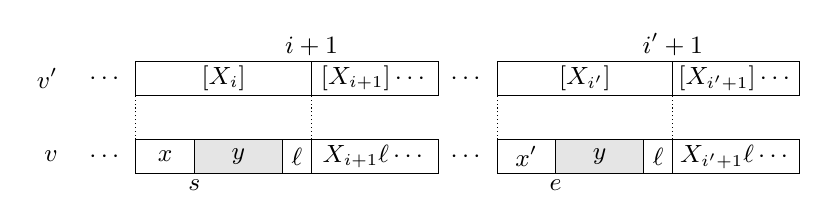
\begin{tikzpicture}[x=0.62cm,y=0.62cm,font=\small]
  % level j+1: the block word
  \node[anchor=east] at (-0.2,1.6) {$v'$};
  \node at (0.6,1.6) {$\cdots$};
  \draw (1.2,1.25) rectangle node{$[X_i]$} (4.8,1.95);
  \draw (4.8,1.25) rectangle node{$[X_{i+1}]\cdots$} (7.4,1.95);
  \node at (8.0,1.6) {$\cdots$};
  \draw (8.6,1.25) rectangle node{$[X_{i'}]$} (12.2,1.95);
  \draw (12.2,1.25) rectangle node{$[X_{i'+1}]\cdots$} (14.8,1.95);
  \node[above,inner sep=2pt] at (4.8,1.95) {$i+1$};
  \node[above,inner sep=2pt] at (12.2,1.95) {$i'+1$};
  % level j: the expansion
  \node[anchor=east] at (-0.2,0) {$v$};
  \node at (0.6,0) {$\cdots$};
  \draw (1.2,-0.35) rectangle node{$x$} (2.4,0.35);
  \draw[fill=black!10] (2.4,-0.35) rectangle node{$y$} (4.2,0.35);
  \draw (4.2,-0.35) rectangle node{$\ell$} (4.8,0.35);
  \draw (4.8,-0.35) rectangle node{$X_{i+1}\ell\cdots$} (7.4,0.35);
  \node at (8.0,0) {$\cdots$};
  \draw (8.6,-0.35) rectangle node{$x'$} (9.8,0.35);
  \draw[fill=black!10] (9.8,-0.35) rectangle node{$y$} (11.6,0.35);
  \draw (11.6,-0.35) rectangle node{$\ell$} (12.2,0.35);
  \draw (12.2,-0.35) rectangle node{$X_{i'+1}\ell\cdots$} (14.8,0.35);
  \node[below,inner sep=2pt] at (2.4,-0.35) {$s$};
  \node[below,inner sep=2pt] at (9.8,-0.35) {$e$};
  \draw[densely dotted] (4.8,0.35) -- (4.8,1.25);
  \draw[densely dotted] (12.2,0.35) -- (12.2,1.25);
  \draw[densely dotted] (1.2,0.35) -- (1.2,1.25);
  \draw[densely dotted] (8.6,0.35) -- (8.6,1.25);
\end{tikzpicture}
\caption{The alignment lemma. Bottom: a comparison $(s,e)$ of the expansion $v$
with $e<\len v$ starts in two blocks $X_i=xy$ and $X_{i'}=x'y$ that have the
common suffix $y$ (shaded) after $s$ and after $e$, so both cuts lie at the same
distance from the markers that close their blocks. Top: what follows these two
markers is the expansion of the block word $v'$ after the cuts $i+1$ and $i'+1$,
so $(s,e)$ is a comparison of $v$ iff, in addition, $(i+1,i'+1)$ is a
comparison of $v'$.}
\Description{Two rows. The top row is the block word with the letters X i,
X i plus one and so on, X i prime, and X i prime plus one and so on; the cuts
after X i and after X i prime are labeled i plus one and i prime plus one. The
bottom row is the expansion: each block X i is drawn as x followed by a shaded
y and the marker, and X i prime as x prime followed by a shaded y and the
marker. The cut s lies before the first shaded y, the cut e before the second.
Dotted lines connect each block of the top row to its expansion.}
\label{fig:bg-alignment}
\end{figure}

For example, the comparison $(0,6)$ of $w=01001101$, with $\wsuf w6=01$,
starts in the blocks $X_0=0$ and $X_3=0$ of $w=(0)1(00)1(\eps)1(0)1$, both at
distance one from their markers and with the common suffix $y=0$, and $(1,4)$ is
the terminal comparison of $w_1=[0][00][\eps][0]$ that ends at its last cut. A
comparison of one level thus reappears at the next level as a comparison of
blocks, together with a test at the same distance from the ends of two blocks.
The derivatives of lettered monitors (\cref{def:bg-derivative}) check
comparisons in exactly this form.

Depth measures how deeply such repetitions are nested. It matters because the
compression behind \cref{thm:bg-search} works one level of the hierarchy at a
time, so its length bound grows with the depth. The depth of a rejected word is
bounded in terms of its rejected tail, for every reader. The key step is the
following lemma.

\begin{lemma}[Return gap {\nssecite{Lemma ``Return gap''}}]\label{lem:bg-return-gap}
Let $w$ be a rejected word of a reader. If $(s,e)$ is a comparison of $w$ and
$q_s=q_e$, then $e-s\le r(w)$.
\end{lemma}
\begin{proof}
Put $\varpi=e-s$. The comparison gives $\wpre ws\,\wsuf we=\wpre w{\len
w-\varpi}$. Since $q_s=q_e$, reading $\wsuf we$ from $q_s$ ends in $q_{\len w}$,
so the state at the cut $\len w-\varpi$ is $q_{\len w}\in\Rej$. By minimality of
$J(w)$, $\len w-\varpi\ge J(w)$, so $\varpi\le r(w)$.
\end{proof}

\begin{theorem}[Depth from the rejected tail {\nssecite{Theorem ``Depth from tail''}}]\label{thm:bg-depth}
For every reader with $N$ states, every nonempty rejected word $w$
satisfies $\depth(w)\le2N(r(w)+1)-1$.
\end{theorem}

\begin{theorem}[Bounded-depth search {\nssecite{Theorem ``Bounded-depth search''}}]\label{thm:bg-search}
Let $(\mathcal M,\Adm,\Rej)$ be a reader with $N$ states over a finite alphabet,
and let $d\ge0$. If it has a nonempty hole of depth at most $d$, then it has a
nonempty hole of depth at most $d$ and length at most $\holeBound(N,d)$, the
explicit elementary function of \cref{eq:bg-len}. The same holds for every
lettered monitor with $N$ states over any alphabet (defined below,
\cref{def:bg-monitor}).
\end{theorem}

\Cref{thm:bg-depth} applies to every nonempty rejected word, whether or not it
is a hole, and neither theorem uses the rejected-path property or a property of
subtype constraints; the alphabet size does not enter the bounds. Combined with
\cref{thm:bg-brt}, they decide the hole problem for readers with the
rejected-path property.

\begin{corollary}[Finite search for holes {\nssecite{Theorem ``Finite search for holes'', Lemma ``Elementary estimate''}}]\label{cor:bg-hole-decision}
Let a reader with $N$ states over a finite alphabet have the rejected-path
property, and put $d_N=2N(4N-1)-1$. It has a hole iff it has a hole of length
at most $\holeBound(N,d_N)$, and $\holeBound(N,d_N)\le2^{2^{1280(N+1)^5}}$.
\end{corollary}
\begin{proof}
By \cref{thm:bg-brt}, some hole $w$ has $r(w)\le4N-2$. If $w$ is empty, it meets
the bound. Otherwise \cref{thm:bg-depth} gives $\depth(w)\le d_N$, and
\cref{thm:bg-search} gives a hole of length at most $\holeBound(N,d_N)$. The
converse is trivial, and the estimate is \cref{lem:bg-estimate}.
\end{proof}

\paragraph{Lettered monitors}
The proof of \cref{thm:bg-search} reads each level of the hierarchy of a hole
with its own automaton, obtained from the automaton of the level below by a
derivative. These automata evaluate their tests at positions inside blocks, so
the tests see the letters as well as the states.

\begin{definition}[Lettered monitor {\nssecite{Sect.\ ``Lettered Monitors and Their Derivatives''}}]\label{def:bg-monitor}
A \emph{lettered monitor} $\mathcal M$ over an alphabet $\Gamma$, possibly
infinite, has a finite state set $\mathcal Q$, a start state $\zeta_0$, a
transition function $\delta:\mathcal Q\times\Gamma\to\mathcal Q$, a
\emph{final-target} predicate $\Tfin\subseteq\mathcal Q\times\Gamma$, and two
relations $\Lambda$ and $\Lfin$ on \emph{labels}, the second for terminal
comparisons. Labels are a symbol $\triangleright$, the \emph{start label}, and
the pairs $(\zeta,a)\in\mathcal Q\times\Gamma$. Reading a word $v$ gives the
states $\zeta_{i+1}=\delta(\zeta_i,v[i])$ and the labels $L_0=\triangleright$
and $L_i=(\zeta_{i-1},v[i-1])$ for $1\le i\le\len v$. A nonempty word $v$ is a
\emph{hole} of $\mathcal M$ if $\Tfin(L_{\len v})$ holds, no terminal comparison
$(s,\len v)$ has $\Lfin(L_s,L_{\len v})$, and no other comparison $(s,e)$ has
$\Lambda(L_s,L_e)$.
\end{definition}

So the label of a cut $i\ge1$ is the last transition before it: the state at
the cut $i-1$ and the letter read from it. A reader $(\mathcal M,\Adm,\Rej)$
with states $Q$, start $q_0$, and transition $\delta$ determines the lettered
monitor with the same states and transitions, $\Tfin(\zeta,a)$ iff
$\delta(\zeta,a)\in\Rej$, and $\Lambda=\Lfin$ given by $\Adm$ on the
\emph{denoted} states, where $\den(\triangleright)=q_0$ and
$\den(\zeta,a)=\delta(\zeta,a)$. Since $\den(L_i)=q_i$, the reader and this
monitor have the same nonempty holes. The tests take labels, and not only the
states they denote, because the monitors of higher levels evaluate them at
positions inside blocks, which requires the letters.

\paragraph{Shifted blocks and derivatives}
Fix a marker $\ell\in\Gamma$, a block $X\in(\Gamma\setminus\{\ell\})^*$, and
$\zeta\in\mathcal Q\sqcup\{\star\}$, where $\star$ is a fresh symbol. The
\emph{shifted block} of $X$ read from $\zeta\in\mathcal Q$ is the word $\ell X$
read from $\zeta$; read from $\star$, it is $X$ read from $\zeta_0$. It has a
label $\lab_g(\zeta,X)$ at each position $g=0,\ldots,\len X$: for
$\zeta\in\mathcal Q$, the label of the cut after $\ell\,\wpre Xg$, so that
position $0$ carries the \emph{marker label} $(\zeta,\ell)$; for $\zeta=\star$,
the label $\triangleright$ at position $0$ and the label of the cut after
$\wpre Xg$ at positions $g\ge1$. The \emph{exit} $\delta_\ell(\zeta,X)\in\mathcal
Q$ is the state at the end of the shifted block. In a word of blocks read by
the derivative below, the \emph{entry state} of a position is the state at the
cut before it, from which the shifted block of its letter is read.

\begin{definition}[Derivative {\nssecite{Definition ``Derivative''}}]\label{def:bg-derivative}
The \emph{derivative} $\mathcal M_\ell$ of $\mathcal M$ along $\ell$ is the
lettered monitor over $(\Gamma\setminus\{\ell\})^*$ with states $\mathcal
Q\sqcup\{\star\}$, start state $\star$, transitions $\delta_\ell$, and
\[
\begin{aligned}
 \Lambda_\ell((\zeta,X),(\zeta',X'))&\iff X=xy,\ X'=x'y,\
   \Lambda\bigl(\lab_{\len x}(\zeta,X),\lab_{\len{x'}}(\zeta',X')\bigr)
   \text{ for some }x,x',y,\\
 \Lfin_\ell((\zeta,X),(\zeta',X'))&\iff \Lambda_\ell((\zeta,X),(\zeta',X'))
   \ \text{or}\ \Lfin\bigl(\lab_g(\zeta,X),(\delta_\ell(\zeta',X'),\ell)\bigr)
   \text{ for some }g\le\len X,\\
 \Tfin_\ell(\zeta,X)&\iff \Tfin(\delta_\ell(\zeta,X),\ell)\ \text{and}\
   \neg\Lfin\bigl(\lab_g(\zeta,X),(\delta_\ell(\zeta,X),\ell)\bigr)
   \text{ for all }g\le\len X;
\end{aligned}
\]
every relation with the start label $\triangleright$ of $\mathcal M_\ell$ as an
argument is false.
\end{definition}

In words: $\Lambda_\ell$ compares two positions at the same distance from the
ends of two blocks, with equal letters after them, as in
\cref{lem:bg-alignment}; the second disjunct of $\Lfin_\ell$ compares a position
anywhere in the block of its first argument with the final cut, which carries
the label of the closing marker; and $\Tfin_\ell$ checks the original target and
all terminal comparisons that start in the last block. Comparisons of the
expansion that start at its cut $0$ are represented inside the first shifted
block, whose entry is $\star$, so setting the relations at the new start label
to false discards none of them.

\paragraph{The label facts}
Let $v=X_0\ell X_1\ell\cdots X_{k-1}\ell$ be the expansion of a nonempty word
$v'=[X_0]\cdots[X_{k-1}]$ of blocks avoiding $\ell$. Let $\zeta'_0=\star$ and
$\zeta'_{i+1}=\delta_\ell(\zeta'_i,X_i)$ be the run of $v'$ in $\mathcal
M_\ell$, put $a_i=\len{X_0\ell\cdots X_{i-1}\ell}$, and let
$b_i=a_i+\len{X_i}$ be the position of the marker closing $X_i$. The intervals
$[a_i,b_i]$ partition the cuts $0,\ldots,\len v-1$, and the labels $L$ of $v$ in
$\mathcal M$ and $L'$ of $v'$ in $\mathcal M_\ell$ satisfy the \emph{label
facts} \nssecite{proof of Lemma ``Holes under desubstitution''}
\begin{equation}\label{eq:bg-label-facts}
 L_{a_i+g}=\lab_g(\zeta'_i,X_i)\quad(0\le g\le\len{X_i}),\qquad
 L_{\len v}=(\zeta'_k,\ell),\qquad
 L'_{i+1}=(\zeta'_i,X_i).
\end{equation}
In particular $\zeta'_{i+1}$ is the state of $\mathcal M$ at the cut $b_i$.

\begin{lemma}[Holes under desubstitution {\nssecite{Lemma ``Holes under desubstitution''}}]\label{lem:bg-desub}
With $v$ and $v'$ as above, $v$ is a hole of $\mathcal M$ iff $v'$ is a hole of
$\mathcal M_\ell$. Consequently, if $\mathcal M_0$ is a lettered monitor with $N$
states and $\mathcal M_{j+1}=(\mathcal M_j)_{\ell_j}$ along the canonical
hierarchy of a nonempty word $w$, then $w$ is a hole of $\mathcal M_0$ iff $w_j$
is a hole of $\mathcal M_j$, for every $j$, and $\mathcal M_j$ has $N+j$
states.
\end{lemma}

\begin{example}[A derivative]
Let a lettered monitor $\mathcal M$ over $\{0,1\}$ read $w=01001101$, with the
state $\zeta_h$ and the label $L_h$ at the cut $h$. With the marker $\ell=1$,
the next level $w_1=[0][00][\eps][0]$ has the blocks $X_0=0$, $X_1=00$,
$X_2=\eps$ and $X_3=0$, which begin at the cuts $0$, $2$, $5$ and $6$ of $w$:
\begin{center}
\small
\begin{tabular}{@{}ccccc@{}}
\toprule
$i$ & $X_i$ & cuts $a_i$--$b_i$ & entry $\zeta'_i$ & label $L'_{i+1}$\\
\midrule
$0$ & $0$ & $0$--$1$ & $\star$ & $(\star,0)$\\
$1$ & $00$ & $2$--$4$ & $\zeta_1$ & $(\zeta_1,00)$\\
$2$ & $\eps$ & $5$ & $\zeta_4$ & $(\zeta_4,\eps)$\\
$3$ & $0$ & $6$--$7$ & $\zeta_5$ & $(\zeta_5,0)$\\
\bottomrule
\end{tabular}
\end{center}
The marker is $1$, so $\mathcal M_1$ is both the derivative along $1$ and the
monitor of level $1$. By the label facts, the run of $w_1$ in $\mathcal M_1$ is
$\star,\zeta_1,\zeta_4,\zeta_5,\zeta_7$, the states before the four markers,
and the labels of $w_1$ are those in the last column; the shifted block of
$X_3$, for instance, is the factor $10$ of $w$ between the cuts $5$ and $7$.

The comparisons of $w_1$ that start after its cut $0$ are the terminal pairs
$(1,4)$, $(2,4)$ and $(3,4)$, which $\mathcal M_1$ tests with $\Lfin_1$. For
$(1,4)$, the first disjunct $\Lambda_1(L'_1,L'_4)$ takes the two common
suffixes $0$ and $\eps$ of $X_0$ and $X_3$ and reads $\Lambda(L_0,L_6)$ and
$\Lambda(L_1,L_7)$: the comparisons $(0,6)$ and $(1,7)$ of $w$
(\cref{fig:bg-alignment}). The second disjunct reads $\Lfin(L_0,L_8)$ and
$\Lfin(L_1,L_8)$: the terminal comparisons of $w$ that start in $X_0$. In the
same way, $(2,4)$ stands for the comparisons $(3,6)$ and $(4,7)$ and for the
terminal comparisons from the cuts $2$, $3$ and $4$, and $(3,4)$ for $(5,7)$
and the terminal comparison from the cut $5$. Finally, $\Tfin_1(L'_4)$ reads
the final target $\Tfin(L_8)$ and excludes the terminal comparisons from the
cuts $6$ and $7$, which start in the last block. These are all the comparisons
of $w$, so $w$ is a hole of $\mathcal M$ iff $w_1$ is a hole of $\mathcal M_1$.
The comparisons $(0,3)$ and $(0,4)$ of $w_1$ start at its start label, where
every relation of $\mathcal M_1$ is false.
\end{example}

\paragraph{How the bounded-depth search works}
Later sections extend the proof of \cref{thm:bg-search}, which has five steps;
\cref{app:bg-search} states them precisely. Let $w$ be a nonempty hole of depth
$D\le d$ with hierarchy $(w_j,\ell_j)$.
\begin{enumerate}[leftmargin=*]
\item \emph{Derivatives.} Let $\mathcal M_0$ be the lettered monitor of the
  reader, and $\mathcal M_{j+1}=(\mathcal M_j)_{\ell_j}$. By
  \cref{lem:bg-desub}, $w_j$ is a hole of $\mathcal M_j$ for every $j$. The
  $N+j$ states of $\mathcal M_j$ are the $N$ \emph{ordinary} states of
  $\mathcal M_0$ and the \emph{symbolic} start states $\star_1,\ldots,\star_j$
  added by the derivatives; ordinary states lead to ordinary states
  (\cref{app:bg-monitors}).
\item \emph{Dictionary normal form.} At each level $1\le i<D$, two isolated
  letters with the same exchange type are merged: the one with the longer
  expansion is replaced by the other, which keeps the comparisons and the
  state run of the level, and the level stays a hole
  (\cref{lem:bg-isolated-exchange}). The result is again a hole of depth $D$,
  no longer. Repeating this bounds the dictionary at every level
  $i\ge1$ by $\mathsf G(N,d)$. The terms are the following.
  \begin{description}[leftmargin=1em,font=\normalfont\itshape]
  \item[Dictionary.] The \emph{dictionary} of level $i$ is the set of letters
    of $w_i$.
  \item[Protected and unprotected letters.] The \emph{protected} letters of
    level $i$ are the marker $\ell_i$ and the letters of the \emph{start
    prefix}, the first at most $i$ positions of $w_i$, which are read from
    symbolic states; every other letter is \emph{unprotected} and is read only
    from ordinary states.
  \item[Isolated letters.] An unprotected letter is \emph{isolated} if all its
    unequal comparison partners are protected: whenever it precedes one cut of
    a comparison and a different letter precedes the other cut, that letter is
    protected.
  \item[Exchange type.] The \emph{exchange type} of an unprotected letter is
    the finite table of how $\mathcal M_i$ treats it when it is read from an
    ordinary state: its transitions and final targets, and the values of
    $\Lambda_i$ and $\Lfin_i$ when it is compared with itself (the \emph{self
    table}), with a protected letter (the \emph{protected rows}), and with the
    start label (the \emph{initial row}).
  \end{description}
\item \emph{The top level.} The unary top level $w_D$ is shortened to at most
  $N+D$ letters by keeping a prefix with the same last label
  (\cref{lem:bg-unary}).
\item \emph{Simultaneous compression.} Going down from the top, the at most
  $\mathsf G(N,d)$ distinct blocks in use at each level are written as the
  tracks of one word of \emph{columns}, aligned at their right ends, and
  shortened together by deleting the columns between two cuts with equal
  \emph{summaries}. The summary of a tuple of blocks records, for every entry
  state, the exit of each block and the final marker labels to which $\Lfin$
  relates its labels, which blocks are equal, and which pairs of blocks the
  derived admission relates; so it determines the derived monitor on the letters in use, and the
  shortened word is again a hole. Precisely, the new derived monitors
  \emph{agree} with the old ones on the letters in use, the \emph{support}: up
  to the renaming of each letter by its shortened version, they have the same
  states, transitions, targets and relations (\cref{eq:bg-agreement}). The
  induction that produces the new markers level by level from the top is the
  \emph{supported compression} of \cref{lem:bg-compression}.
\item \emph{The bound.} Each shortened block has fewer than
  $\mathsf{col}(N+d+1,\mathsf G(N,d))$ letters, so each of the at most $d$
  expansions multiplies the length by at most this factor. With the top level
  this gives $\holeBound(N,d)$.
\end{enumerate}
Shortening each block separately would fail, because comparisons relate
different blocks through equal suffixes. The compression keeps a word a hole,
that is, it preserves the absence of admitted comparisons, but it may destroy
any particular comparison; positive conditions need the extension of
\cref{sec:mo}.

%% leaf -- signed leaf cones: the representation and the order, the clause
%% form of every literal, least closures with one seed per atom, duality,
%% extensions first, and collision return. Long proofs are in appendix-leaf.

\section{Signed Leaf Cones}\label{sec:lf}

This section represents trees, and the solutions of systems, by sets of
propositional atoms. In these coordinates every system over $\BFT$, of any
arity and any variance, becomes a set of Horn clauses: implications with one
premise, unit clauses (facts and forbidden roots), and one fixed family of binary
exclusions. The representation has two consequences on which the rest of the
paper rests. Least solutions are computed by closing a set of seeds, and every
atom of a closure has a single seed (\cref{sec:lf-least}). Every pure move
has a dual with both signs flipped, so two derivations that collide can be
merged into one (\cref{sec:lf-duality}).

We use the notation of \cref{sec:bg-trees,sec:bg-constraints}, in
particular the directions $\Sigma=\{0,\dots,n-1\}$, the variance $c$, the
polarity $\parity(w)$, the order $\le_c$, the normalizations $\nu_s$, the dual
$t^\partial$ and the full constructor tree $\Omega$, and we put
$\Sigma^+=\Sigma^*\setminus\{\eps\}$.
In this section and the next, all trees are trees over $\BFT$, and
assignments range over arbitrary trees; regular and finite trees are treated
in \cref{sec:tc}. Proofs omitted here are in \cref{app:lf}.

The positions of a tree $t$ labeled $\Bot$ or $\Top$ are its \emph{leaves}. We
use the \emph{chain property}: for every tree $t$ and every word $w$, at most
one prefix of $w$ is a leaf of $t$, and if none is, then $w$ is a position of
$t$ labeled $f$. Indeed, by induction on its prefixes, a prefix of $w$ is a
position as long as no shorter prefix is a leaf, and a position that is not a
leaf has all its children.

\subsection{Leaf Cones}\label{sec:lf-cones}

\begin{definition}[Signed leaf cones]\label{def:lf-cones}
For a tree $T$, the \emph{top-leaf cone} $A_T$ is the set of words $w$ such
that some prefix of $w$ is a position of $T$ labeled $\Top$. For a tree $t$
and a sign $s\in\{0,1\}$, the \emph{leaf cone of sign $s$} of $t$ is
\[
 L^s_t=A_{\nu_st}.
\]
We also write $L^+_t=L^0_t$ and $L^-_t=L^1_t$, and call $(L^0_t,L^1_t)$ the
\emph{leaf pair} of $t$.
\end{definition}

The cones have a direct description. The \emph{sign} of a leaf $v$ of $t$ is
$b\oplus\parity(v)$, where $b=0$ if $t(v)=\Top$ and $b=1$ if $t(v)=\Bot$.
The tree $\nu_st$ carries the label $\Top$ at a leaf $v$ iff $v$ has sign $s$.
By the chain property, therefore,
\begin{equation}\label{eq:lf-direct}
 w\in L^s_t\quad\Longleftrightarrow\quad
 \text{the path $w$ meets a leaf of $t$ of sign $s$.}
\end{equation}
Since $\nu_1t=(\nu_0t)^\partial$ (\cref{lem:bg-normalization}(1)), the cone
$L^1_t$ is the bottom-leaf cone of $\nu_0t$: the two cones belong to the same normalized tree. The variance
enters only through the sign of each leaf, and the parity that determines this
sign accumulates along the path and stops at the leaf. There are two cones per
tree, whatever the arity, not one per assignment of signs to the children.
In terms of the signed correspondence (\cref{lem:bg-signed}),
$L^s_{\rho(v)}$ is the top-leaf cone of the covariant tree $\rho^\pm(v^s)$.

\begin{theorem}[Leaf representation]\label{thm:lf-representation}
\leavevmode
\begin{enumerate}[leftmargin=*]
\item For every tree $t$, the sets $L^0_t$ and $L^1_t$ are disjoint, and each
  is \emph{extension closed}: $w\in L^s_t$ implies $wi\in L^s_t$ for every
  letter $i$. Conversely, every pair $(L^0,L^1)$ of disjoint extension-closed
  sets of words is the leaf pair of exactly one tree.
\item For all trees $t$ and $u$,
  \[
   t\le_c u\quad\Longleftrightarrow\quad
   L^0_t\subseteq L^0_u\ \text{ and }\ L^1_u\subseteq L^1_t .
  \]
\item $L^0_\Top=L^1_\Bot=\Sigma^*$, $L^1_\Top=L^0_\Bot=\varnothing$, and
  $L^s_{t^\partial}=L^{1-s}_t$. If $t=f(t_i)_i$, then neither cone of $t$
  contains $\eps$, and for every letter $i$, word $w$, and sign $s$,
  \[
   iw\in L^s_t\quad\Longleftrightarrow\quad w\in L^{s\oplus c(i)}_{t_i}.
  \]
  In particular, $\eps\in L^0_t$ iff $t=\Top$, and $\eps\in L^1_t$ iff
  $t=\Bot$.
\item The positions of $t$ labeled $f$ are exactly the words outside
  $L^0_t\cup L^1_t$. Hence $t$ is finite iff
  $\Sigma^*\setminus(L^0_t\cup L^1_t)$ is finite, and $t$ is regular iff
  $L^0_t$ and $L^1_t$ are regular languages.
\end{enumerate}
\end{theorem}

By (2), the order adds leaves of sign $0$ and removes leaves of sign $1$ as
it goes up: after normalization, larger trees have more top leaves and fewer
bottom leaves. The order is therefore not the inclusion of both cones.
Inclusion of both cones is an \emph{information order}, whose least element
is the tree without leaves, $\Omega$, with the leaf pair
$(\varnothing,\varnothing)$. The least solutions of \cref{sec:lf-least} are
least in the information order.

\begin{example}[Leaf cones of arrows]\label{ex:lf-arrow}
For the arrow, $n=2$ and $f(a_0,a_1)=a_0\to a_1$ with $c(0)=1$ and $c(1)=0$, so
$\parity(w)$ is the parity of the number of letters $0$ in $w$. The leaf pairs
of $\Top$, $\Bot$ and $\Omega$ are $(\Sigma^*,\varnothing)$,
$(\varnothing,\Sigma^*)$ and $(\varnothing,\varnothing)$. In $\Top\to\Bot$, the
leaf $0$ is labeled $\Top$ and has polarity $1$, and the leaf $1$ is labeled
$\Bot$ and has polarity $0$; both have sign $1$, so the leaf pair is
$(\varnothing,\Sigma^+)$. Likewise $\Bot\to\Top$ has the leaf pair
$(\Sigma^+,\varnothing)$, and $\Bot\to\Omega$ has $(0\Sigma^*,\varnothing)$. By
\cref{thm:lf-representation}(3), both cones of every tree $f(a_0,a_1)$ lie in
$\Sigma^+$, so (2) gives $\Top\to\Bot\le_c f(a_0,a_1)\le_c\Bot\to\Top$: these
are the least and the greatest arrow types.
\end{example}

\Cref{fig:lf-cones} follows three arrow types up to the greatest one,
$\Bot\to\Top$. The sign of each leaf is read off its label and its path, and
each step up either removes a leaf of sign~$1$ or adds a leaf of sign~$0$, even
where a subtree at a contravariant position becomes smaller.

\begin{figure}[tbp]
\centering
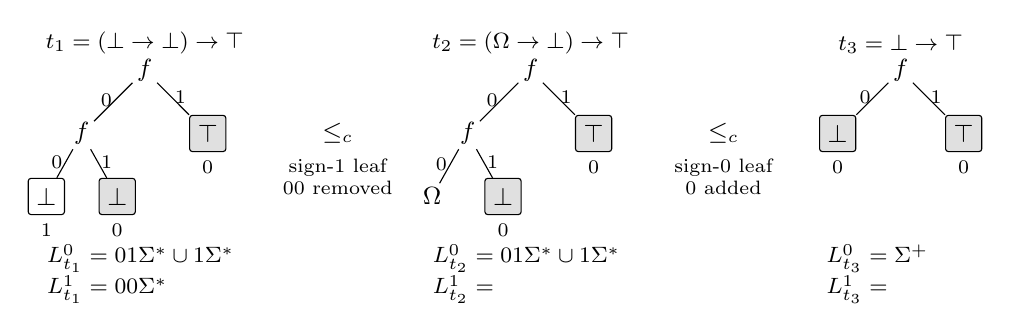
\begin{tikzpicture}[>=Stealth,font=\small,
    every node/.style={inner sep=1.5pt},
    tree/.style={level distance=8mm,
      level 1/.style={sibling distance=16mm},
      level 2/.style={sibling distance=9mm}},
    e0/.style={left,font=\scriptsize,inner sep=1pt,pos=0.45},
    e1/.style={right,font=\scriptsize,inner sep=1pt,pos=0.45},
    s0/.style={draw,rounded corners=1pt,fill=black!12,minimum size=4.6mm},
    s1/.style={draw,rounded corners=1pt,minimum size=4.6mm},
    sg/.style={below=0.5mm,font=\scriptsize},
    lb/.style={font=\footnotesize,align=left,anchor=north west}]
  % t1 = (Bot -> Bot) -> Top
  \begin{scope}[tree]
    \node at (1.3,0) {$f$}
      child {node {$f$}
        child {node[s1] (l00) {$\Bot$} edge from parent node[e0]{0}}
        child {node[s0] (l01) {$\Bot$} edge from parent node[e1]{1}}
        edge from parent node[e0]{0}}
      child {node[s0] (l1) {$\Top$} edge from parent node[e1]{1}};
  \end{scope}
  \node[sg] at (l00.south) {$1$};
  \node[sg] at (l01.south) {$0$};
  \node[sg] at (l1.south) {$0$};
  \node[font=\footnotesize,anchor=south] at (1.3,0.15) {$t_1=(\Bot\to\Bot)\to\Top$};
  \node[lb] at (0.0,-2.15) {$L^0_{t_1}=01\Sigma^*\cup1\Sigma^*$\\ $L^1_{t_1}=00\Sigma^*$};
  % t2 = (Omega -> Bot) -> Top
  \begin{scope}[tree]
    \node at (6.2,0) {$f$}
      child {node {$f$}
        child {node (o00) {$\Omega$} edge from parent node[e0]{0}}
        child {node[s0] (m01) {$\Bot$} edge from parent node[e1]{1}}
        edge from parent node[e0]{0}}
      child {node[s0] (m1) {$\Top$} edge from parent node[e1]{1}};
  \end{scope}
  \node[sg] at (m01.south) {$0$};
  \node[sg] at (m1.south) {$0$};
  \node[font=\footnotesize,anchor=south] at (6.2,0.15) {$t_2=(\Omega\to\Bot)\to\Top$};
  \node[lb] at (4.9,-2.15) {$L^0_{t_2}=01\Sigma^*\cup1\Sigma^*$\\ $L^1_{t_2}=\varnothing$};
  % t3 = Bot -> Top
  \begin{scope}[tree]
    \node at (10.9,0) {$f$}
      child {node[s0] (n0) {$\Bot$} edge from parent node[e0]{0}}
      child {node[s0] (n1) {$\Top$} edge from parent node[e1]{1}};
  \end{scope}
  \node[sg] at (n0.south) {$0$};
  \node[sg] at (n1.south) {$0$};
  \node[font=\footnotesize,anchor=south] at (10.9,0.15) {$t_3=\Bot\to\Top$};
  \node[lb] at (9.9,-2.15) {$L^0_{t_3}=\Sigma^+$\\ $L^1_{t_3}=\varnothing$};
  % the order
  \node at (3.75,-0.8) {$\le_c$};
  \node[font=\scriptsize,align=center] at (3.75,-1.35) {sign-$1$ leaf\\ $00$ removed};
  \node at (8.65,-0.8) {$\le_c$};
  \node[font=\scriptsize,align=center] at (8.65,-1.35) {sign-$0$ leaf\\ $0$ added};
\end{tikzpicture}
\caption{Signed leaf cones of three arrow types, $c(0)=1$ and $c(1)=0$. The
number below a leaf is its sign: $0$ for $\Top$ and $1$ for $\Bot$, plus the
number of letters $0$ on its path, modulo two. Leaves of sign $0$ are shaded;
the leaf $\Bot$ at $01$ has sign $0$, and so does the leaf $\Bot$ at $0$ in
$t_3$. Going up in the order removes leaves of sign $1$ and adds leaves of sign
$0$ (\cref{thm:lf-representation}(2)): $t_1\le_ct_2$ shrinks $L^1$, and
$t_2\le_ct_3$ grows $L^0$ by replacing the subtree $\Omega\to\Bot$ at the
contravariant position $0$ with the smaller tree $\Bot$.}
\Description{Three trees side by side, separated by the symbol less or equal
for the variance c. Left: the arrow type from bottom to bottom, to top; its
leaves are bottom at 00 with sign 1, bottom at 01 with sign 0, and top at 1
with sign 0. Middle: the same tree with Omega in place of the leaf at 00; its
leaves bottom at 01 and top at 1 both have sign 0. Right: bottom to top, whose
two leaves have sign 0. Under each tree its two leaf cones are listed: zero one
Sigma star union one Sigma star and zero zero Sigma star; zero one Sigma star
union one Sigma star and the empty set; Sigma plus and the empty set. Leaves of
sign 0 are shaded. Between the first two trees: sign 1 leaf 00 removed; between
the last two: sign 0 leaf 0 added.}
\label{fig:lf-cones}
\end{figure}


\subsection{Atoms and Clauses}\label{sec:lf-clauses}

Let $V$ be a finite set of variables, and recall the signed variables $v^s$,
their set $V^\pm$, and the flip $\overline{v^s}=v^{1-s}$
(\cref{sec:bg-constraints}); we put $\sgn(v^s)=s$. An \emph{atom} is a pair
$(p,w)\in\Conf_V=V^\pm\times\Sigma^*$, and its \emph{opposite} is
$\overline{(p,w)}=(\bar p,w)$. An assignment $\rho$ of trees to $V$
determines the set of atoms
\[
 S_\rho=\{(v^s,w):w\in L^s_{\rho(v)}\},
\]
and an atom \emph{holds} in $\rho$ if it lies in $S_\rho$. An atom of sign
$0$ is \emph{positive}, and an atom of sign $1$ is \emph{negative}. Opposite atoms are
incompatible but not complementary: in $\Omega$ neither holds. For
$U\subseteq V$ and $S\subseteq\Conf_V$ we put $S|_U=S\cap\Conf_U$. We read
the word of an atom as a stack whose top is its first letter.

A set $S$ of atoms is \emph{extension closed} if $(p,w)\in S$ implies
$(p,wi)\in S$ for every letter $i$, and an \emph{exclusion pair} of $S$ is a
pair $a,\bar a$ of opposite atoms that both lie in $S$. By
\cref{thm:lf-representation}(1), applied to each variable, $\rho\mapsto
S_\rho$ is a bijection from the assignments of trees to $V$ onto the
extension-closed subsets of $\Conf_V$ without exclusion pairs.

\begin{table}[t]
\caption{The clause form of a literal, for all words $w$ and all letters
$i\in\Sigma$; here $\bar c(i)=1\oplus c(i)$. Every system also has the
extensions $(p,w)\to(p,wi)$ for all $p\in V^\pm$, $w\in\Sigma^*$ and
$i\in\Sigma$.}
\label{tab:lf-clauses}
\centering
\begin{tabular}{@{}lll@{}}
\toprule
Literal & Pure moves & Root unit\\
\midrule
$u\le v$ & copies: $(u^0,w)\to(v^0,w)$ and $(v^1,w)\to(u^1,w)$ & none\\[2pt]
$f(a_i)_i\le u$ & $\mathrm{push}_i$: $(a_i^{c(i)},w)\to(u^0,iw)$
 & forbidden root $(u^1,\eps)$\\
 & $\mathrm{pop}_i$: $(u^1,iw)\to(a_i^{\bar c(i)},w)$ & \\[2pt]
$u\le f(a_i)_i$ & $\mathrm{pop}_i$: $(u^0,iw)\to(a_i^{c(i)},w)$
 & forbidden root $(u^0,\eps)$\\
 & $\mathrm{push}_i$: $(a_i^{\bar c(i)},w)\to(u^1,iw)$ & \\[2pt]
$u=\Bot$ & none & fact $(u^1,\eps)$\\
$\Top\le u$ & none & fact $(u^0,\eps)$\\
\bottomrule
\end{tabular}
\end{table}

The literals of a system $\chi$ over $V$ determine the \emph{pure moves},
\emph{facts} and \emph{forbidden roots} listed in
\cref{tab:lf-clauses}; facts and forbidden roots are the unit clauses. A push or a pop of direction $i$ changes the sign by
$c(i)$, and a copy keeps it. The \emph{rules} of $\chi$ are its pure moves and
the \emph{extensions} $(p,w)\to(p,wi)$. We write $\Fact_\chi$ and $\Neg_\chi$
for the sets of facts and forbidden roots. Pure moves read and write
only the top of the stack: $\mathrm{push}_i$ puts the letter $i$ on top,
$\mathrm{pop}_i$ removes it, and a copy leaves the stack unchanged. They form a
pushdown system with control states $V^\pm$ and stack alphabet $\Sigma$,
which \cref{sec:sm} summarizes by finite automata. Extensions, in contrast,
add a letter at the bottom of the stack.

The table is the signed system $\chi^\pm$ of \cref{tab:bg-signed} read in
top-leaf cones. Every copy literal $p\le q$ of $\chi^\pm$ gives the pure moves
$(p,w)\to(q,w)$, every lower constructor literal $f(p_i)_i\le q$ gives
$(p_i,w)\to(q,iw)$, and every upper constructor literal $q\le f(p_i)_i$ gives
$(q,iw)\to(p_i,w)$. The forbidden roots are the atoms $(q,\eps)$ for the roots
$q$ of the upper constructor literals of $\chi^\pm$, and the facts
are the atoms $(q,\eps)$ for its literals $\Top\le q$.

\begin{definition}[Models]\label{def:lf-model}
A set $S\subseteq\Conf_V$ is \emph{consistent} for $\chi$ if it contains no
forbidden root of $\chi$ and no exclusion pair. A \emph{model} of $\chi$ is a
consistent set of atoms that contains $\Fact_\chi$ and is closed under all
rules of $\chi$. We write $\Mod(\chi)$ for the set of models of $\chi$.
\end{definition}

\begin{lemma}[Clause form]\label{lem:lf-clauses}
An assignment $\rho$ satisfies a literal iff $S_\rho$ is closed under the
pure moves of the literal, contains its facts, and contains none of
its forbidden roots. Consequently, $\rho\mapsto S_\rho$ is a bijection from
the solutions of $\chi$ onto $\Mod(\chi)$.
\end{lemma}

The proof (\cref{app:lf}) substitutes the identities of
\cref{thm:lf-representation}(3) into the inclusions of
\cref{thm:lf-representation}(2). Every literal thus contributes implications
with one premise and units only; the only all-negative binary clauses are the
exclusions $\neg(a\wedge\bar a)$, which are the same for all systems, and no
clause is a positive disjunction. A constructor literal contributes $2n$
schemes of pure moves and one forbidden root, and a copy literal two schemes.
For $n=0$, the literal $f()\le u$ says $u\ne\Bot$ and $u\le f()$ says
$u\ne\Top$.

We write $a\to_\chi b$ if a pure move of $\chi$ leads from $a$ to $b$.

\begin{lemma}[Pure moves]\label{lem:lf-moves}
Let $(p,u)\to_\chi(q,t)$.
\begin{enumerate}[leftmargin=*]
\item For every word $\sigma$, $(p,u\sigma)\to_\chi(q,t\sigma)$, by the same
  scheme of \cref{tab:lf-clauses}.
\item $\sgn(q)\oplus\parity(t)=\sgn(p)\oplus\parity(u)$.
\end{enumerate}
\end{lemma}

Item (1) holds because each scheme is stated for all words $w$, and (2) is a
direct check of the six schemes (\cref{app:lf}). Both extend to sequences
of pure moves. By (2), along such a sequence the sign of the current signed
variable is determined by the first atom and the parity of the current word;
we call (2) the \emph{sign invariant}.

\begin{example}[The system $x\le x\to x$]\label{ex:lf-clauses}
Let $\varphi=\{x\le x\to x\}$ for the arrow of \cref{ex:lf-arrow}, that is,
the literal $x\le f(x,x)$. By \cref{tab:lf-clauses}, its pure moves are
\[
\begin{array}{ll}
 \mathrm{pop}_0:\ (x^0,0w)\to(x^1,w), & \mathrm{push}_0:\ (x^0,w)\to(x^1,0w),\\
 \mathrm{pop}_1:\ (x^0,1w)\to(x^0,w), & \mathrm{push}_1:\ (x^1,w)\to(x^1,1w),
\end{array}
\]
it has the forbidden root $(x^0,\eps)$, and it has no facts. A move
in the contravariant direction $0$ changes the sign, and a move in the
covariant direction $1$ keeps it. In each row, the push is the pop read
backwards with both signs reversed; \cref{lem:lf-duality} shows that this
holds for every system. The tree $\Top\to\Bot$, with leaf pair
$(\varnothing,\Sigma^+)$, is a solution: its atoms are the $(x^1,w)$ with
$w\ne\eps$, and this set is closed under $\mathrm{push}_1$ and under
extensions.
\end{example}

\subsection{Least Closures}\label{sec:lf-least}

A \emph{derivation} of $\chi$ is a finite sequence of atoms $a_0,\dots,a_k$,
with $k\ge0$, in which each $a_{j+1}$ follows from $a_j$ by a rule of $\chi$;
it is \emph{pure} if all its rules are pure moves. We write
$a\Rightarrow^*_\chi b$ if a derivation leads from $a$ to $b$, and
$a\to^*_\chi b$ if a pure derivation does; we drop the subscript when $\chi$
is clear. For an atom $a$ and a set $A$ of atoms put
\[
 \Reach_\chi(a)=\{b:a\Rightarrow^*_\chi b\},\qquad
 \mu_\chi=\bigcup_{e\in\Fact_\chi}\Reach_\chi(e),\qquad
 H_\chi(A)=\mu_\chi\cup\bigcup_{a\in A}\Reach_\chi(a),
\]
and $\Cl_\chi(a)=H_\chi(\{a\})$. An atom is \emph{live} in $\chi$ if some
model of $\chi$ contains it, and \emph{dead} otherwise; $\Live_\chi$ is the
set of live atoms. Every rule has a single premise, so every atom $b$ of
$H_\chi(A)$ has a \emph{seed}: an atom $x\in\Fact_\chi\cup A$ with
$b\in \Reach_\chi(x)$.

\begin{lemma}[Least closures]\label{lem:lf-closure}\label{lem:lf-least}
Let $\chi$ be a system over $V$ and $A\subseteq\Conf_V$.
\begin{enumerate}[leftmargin=*]
\item $H_\chi(A)$ is the least set of atoms that contains $\Fact_\chi\cup A$
  and is closed under the rules of $\chi$.
\item Some model of $\chi$ contains $A$ iff $H_\chi(A)$ is consistent, and
  then $H_\chi(A)$ is the least model that contains $A$. In particular,
  $\chi$ is satisfiable iff $\mu_\chi$ is consistent, and then $\mu_\chi$ is
  the least model of $\chi$; and an atom $a$ is live iff $\Cl_\chi(a)$ is
  consistent, and then $\Cl_\chi(a)$ is the least model that contains $a$.
\item If $H_\chi(A)$ is not consistent, then there are seeds
  $x,y\in\Fact_\chi\cup A$, possibly equal, such that $\Reach_\chi(x)$ contains a
  forbidden root, or $b\in \Reach_\chi(x)$ and $\bar b\in \Reach_\chi(y)$ for some atom
  $b$.
\item For every atom $(p,u)$ and every word $\alpha$,
  $(p,u\alpha)\in \Reach_\chi(p,u)$; hence
  $\Cl_\chi(p,u\alpha)\subseteq\Cl_\chi(p,u)$, and if $(p,u)$ is live, then
  so is $(p,u\alpha)$.
\item Let $V=X\cup Z$ with $X\cap Z=\varnothing$, and let $S\subseteq\Conf_X$
  be extension closed and without exclusion pairs. Then $S=T|_X$ for some
  model $T$ of $\chi$ iff $H_\chi(S)$ is consistent and $H_\chi(S)|_X=S$; in
  this case $H_\chi(S)$ is the least such model.
\end{enumerate}
\end{lemma}

Item (3) says that every inconsistency has at most two seeds; it bounds
neither the words of the seeds nor the lengths of the derivations. Item (5)
reduces the extension of a given visible assignment to a single closure;
\cref{thm:ch-characterization} and the transfers of \cref{sec:tc} use the
lemma in this form.

\begin{example}[Liveness in $x\le x\to x$]\label{ex:lf-least}
We continue \cref{ex:lf-clauses}. The system $\varphi$ has no facts,
so $\mu_\varphi=\varnothing$ is consistent: $\varphi$ is satisfiable, and its
least solution is $x=\Omega$. Every atom $(x^1,u)$ is live, since the
solution $x=\Bot$ contains it. The atoms $(x^0,1^k)$ are dead: $k$ pops in
direction $1$ lead to the forbidden root $(x^0,\eps)$. The atom $(x^0,0)$ is
dead for a different reason. The pop $(x^0,0)\to(x^1,\eps)$ followed by an
extension derives $(x^1,0)$, the opposite of the seed, so
$\Cl_\varphi((x^0,0))$ contains an exclusion pair. No forbidden root is
derivable from $(x^0,0)$: the only atoms $(x^0,w)$ that it derives are its
extensions $(x^0,0w)$, and no move leads from a negative atom of $x$ to a
positive one. So this inconsistency has a single seed and uses no unit.
Finally, $(x^0,01)$ is live: its least model is the solution
$((\Omega\to\Bot)\to\Bot)\to\Bot$, whose atoms are the $(x^0,w)$ with
$w\in01\Sigma^*$ and the $(x^1,w)$ with $w\in1^+\Sigma^*\cup1^*001\Sigma^*$.
\end{example}

\Cref{fig:lf-moves}(a) draws these derivations with each atom at the height of
its word, so that the moves act as on a stack: pops go down, pushes go up, and
an extension adds a letter at the bottom without changing the top.

\begin{figure}[tbp]
\centering
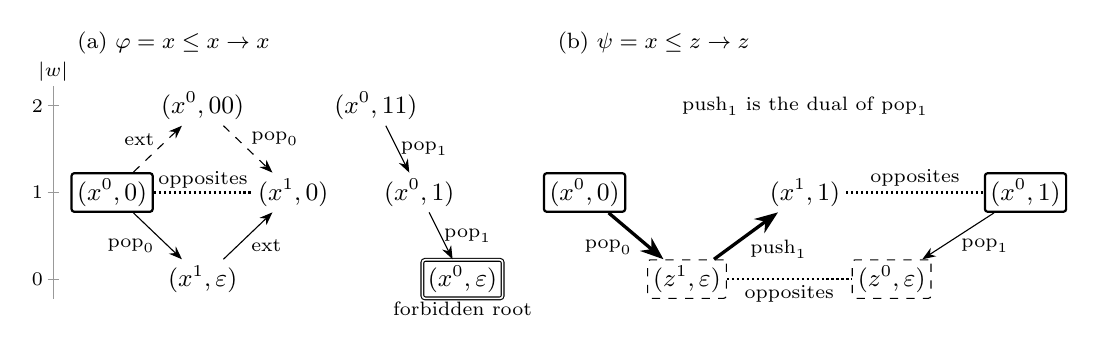
\begin{tikzpicture}[>=Stealth,font=\small,x=1cm,y=1cm,
    every node/.style={inner sep=1.5pt},
    atom/.style={inner sep=2pt},
    seed/.style={atom,draw,thick,rounded corners=1pt},
    hidden/.style={atom,draw,dashed,rounded corners=1pt},
    mv/.style={->},
    ml/.style={font=\scriptsize,inner sep=1pt},
    opp/.style={densely dotted,thick}]
  % height axis
  \draw[black!40] (-0.75,-0.25) -- (-0.75,2.45);
  \foreach \h/\y in {0/0,1/1.1,2/2.2}
    {\draw[black!40] (-0.82,\y) -- (-0.68,\y);
     \node[font=\scriptsize,anchor=east] at (-0.82,\y) {$\h$};}
  \node[font=\scriptsize,anchor=south] at (-0.75,2.45) {$\len w$};
  % (a) phi = x <= x -> x
  \node[font=\footnotesize,anchor=west] at (-0.5,3.0) {(a) $\varphi=x\le x\to x$};
  \node[seed] (s) at (0,1.1) {$(x^0,0)$};
  \node[atom] (p) at (1.15,0) {$(x^1,\eps)$};
  \node[atom] (o) at (2.3,1.1) {$(x^1,0)$};
  \node[atom] (e) at (1.15,2.2) {$(x^0,00)$};
  \draw[mv] (s) -- node[ml,below left]{$\mathrm{pop}_0$} (p);
  \draw[mv] (p) -- node[ml,below right]{ext} (o);
  \draw[mv,dashed] (s) -- node[ml,above left]{ext} (e);
  \draw[mv,dashed] (e) -- node[ml,above right]{$\mathrm{pop}_0$} (o);
  \draw[opp] (s) -- node[ml,above,fill=white]{opposites} (o);
  \node[atom] (r2) at (3.35,2.2) {$(x^0,11)$};
  \node[atom] (r1) at (3.9,1.1) {$(x^0,1)$};
  \node[atom,draw,double,rounded corners=1pt] (r0) at (4.45,0) {$(x^0,\eps)$};
  \draw[mv] (r2) -- node[ml,right]{$\mathrm{pop}_1$} (r1);
  \draw[mv] (r1) -- node[ml,right]{$\mathrm{pop}_1$} (r0);
  \node[ml,anchor=north] at (4.45,-0.25) {forbidden root};
  % (b) psi = x <= z -> z
  \node[font=\footnotesize,anchor=west] at (5.6,3.0) {(b) $\psi=x\le z\to z$};
  \node[seed] (a) at (6.0,1.1) {$(x^0,0)$};
  \node[seed] (b) at (11.6,1.1) {$(x^0,1)$};
  \node[hidden] (z1) at (7.3,0) {$(z^1,\eps)$};
  \node[hidden] (z0) at (9.9,0) {$(z^0,\eps)$};
  \node[atom] (xb) at (8.8,1.1) {$(x^1,1)$};
  \draw[mv,very thick] (a) -- node[ml,below left]{$\mathrm{pop}_0$} (z1);
  \draw[mv] (b) -- node[ml,below right]{$\mathrm{pop}_1$} (z0);
  \draw[mv,very thick] (z1) -- node[ml,below right]{$\mathrm{push}_1$} (xb);
  \draw[opp] (z1) -- node[ml,below=1pt]{opposites} (z0);
  \draw[opp] (xb) -- node[ml,above=1pt]{opposites} (b);
  \node[ml,align=center] at (8.8,2.2) {$\mathrm{push}_1$ is the dual of $\mathrm{pop}_1$};
\end{tikzpicture}
\caption{Pure moves and extensions for the arrow, with each atom drawn at the
height $\len w$ of its word: a pop lowers the stack, a push raises it, and an
extension adds a letter at the bottom. Seeds are framed, hidden atoms dashed.
(a) In $x\le x\to x$ (\cref{ex:lf-clauses,ex:lf-least}), the seed $(x^0,0)$
derives its own opposite $(x^1,0)$, by a pop and an extension or, dashed, with
the extension first (\cref{lem:lf-ext-first}): a single-seed inconsistency
without any unit. The atom $(x^0,11)$ is dead for a different reason: it pops
down to the forbidden root $(x^0,\eps)$. (b) In $x\le z\to z$
(\cref{ex:ch-arrow}), the seeds $(x^0,0)$ and $(x^0,1)$ derive the opposite
atoms $(z^1,\eps)$ and $(z^0,\eps)$ of the hidden $z$. Reversing the second
branch with flipped signs (\cref{lem:lf-duality}) continues the first one (thick):
the single seed $(x^0,0)$ derives $(x^1,1)$, the opposite of the second seed,
which is collision return (\cref{lem:lf-collision}).}
\Description{Two panels of atoms placed at heights 0, 1 and 2, the length of
their words. Panel a: the framed seed x zero at word 0 pops to x one at the
empty word, which extends to x one at word 0, drawn at the height of the seed
and joined to it by a dotted line labeled opposites; a dashed route first extends the seed to x
zero at 00 and then pops to the same atom. To the right, x zero at 11 pops
twice to the doubly framed forbidden root x zero at the empty word. Panel b:
the framed seeds x zero at 0 and x zero at 1 pop to the dashed hidden atoms z
one and z zero at the empty word, joined by a dotted line labeled opposites;
a thick push in direction 1 leads from z one to x one at word 1, which is
joined by a dotted line to the second seed.}
\label{fig:lf-moves}
\end{figure}


\subsection{Duality, Extensions First, and Collision Return}\label{sec:lf-duality}

\begin{lemma}[Duality]\label{lem:lf-duality}
If $a\to_\chi b$, then $\bar b\to_\chi\bar a$. Consequently, $a\to^*_\chi b$
implies $\bar b\to^*_\chi\bar a$.
\end{lemma}

\begin{proof}
By \cref{tab:lf-clauses}: the two copies of a literal $u\le v$ are each
other's duals, and so are $\mathrm{push}_i$ and $\mathrm{pop}_i$ of the same
constructor literal, for each direction $i$ separately; for instance, the
dual of $(a_i^{c(i)},w)\to(u^0,iw)$ is $(u^1,iw)\to(a_i^{\bar c(i)},w)$.
This holds also when variables are repeated among $u,a_0,\dots,a_{n-1}$,
since the pairing is by scheme. For derivations, reverse the sequence and
dualize each move.
\end{proof}

Extensions have no duals: the reverse of an extension would delete the
bottom letter of a stack, and no rule does that. The next lemma moves all
extensions of a derivation to its beginning, so that duality applies to the
rest.

\begin{lemma}[Extensions first]\label{lem:lf-ext-first}\label{lem:lf-extensions}
For all atoms $(p,u)$ and $b$, $b\in \Reach_\chi(p,u)$ iff
$(p,u\alpha)\to^*_\chi b$ for some word $\alpha$.
\end{lemma}

The proof (\cref{app:lf}) inducts on the derivation: an extension at the
end appends a letter to the bottom of every stack of the pure derivation
obtained so far, which \cref{lem:lf-moves}(1) allows.

\begin{lemma}[Collision return]\label{lem:lf-collision}
Let $a$ and $(q,v)$ be atoms. If $b\in \Reach_\chi(a)$ and $\bar b\in \Reach_\chi(q,v)$
for some atom $b$, then $(\bar q,v\delta)\in \Reach_\chi(a)$ for some word
$\delta$. If moreover $a=(p,u)$, then
$(p,u\alpha)\to^*_\chi(\bar q,v\delta)$ for some words $\alpha$ and $\delta$.
\end{lemma}

\begin{proof}
By \cref{lem:lf-ext-first}, $(q,v\delta)\to^*\bar b$ for some $\delta$, and by
\cref{lem:lf-duality}, $b\to^*(\bar q,v\delta)$. Appending this pure
derivation to a derivation from $a$ to $b$ gives
$(\bar q,v\delta)\in \Reach_\chi(a)$. For the second claim apply
\cref{lem:lf-ext-first} to this membership.
\end{proof}

Thus two derivations that end in an exclusion pair, possibly at a hidden
variable, merge into one derivation from the first seed to the opposite of
an extension of the second seed (\cref{fig:lf-moves}(b)): the first
derivation continues along the second one, read backwards with flipped signs.
The extension is necessary: in general the
merged derivation does not reach the opposite of the second seed itself
(\cref{ex:ch-arrow}). The first consequence concerns a single seed.

\begin{corollary}[Deadness]\label{cor:lf-dead}
Let $\chi$ be satisfiable and let $(p,u)$ be an atom. Then $(p,u)$ is dead
in $\chi$ iff at least one of the following holds:
\begin{enumerate}[label=(\alph*),leftmargin=*]
\item $\Reach_\chi(p,u)$ contains a forbidden root;
\item $(\bar p,u\delta)\in\mu_\chi$ for some word $\delta$;
\item $(\bar p,u\delta)\in \Reach_\chi(p,u)$ for some word $\delta$.
\end{enumerate}
Moreover, (a) holds iff $(p,u\alpha)\to^*_\chi e$ for some word $\alpha$ and
some $e\in\Neg_\chi$, and (c) holds iff
$(p,u\alpha)\to^*_\chi(\bar p,u\delta)$ for some words $\alpha$ and $\delta$.
\end{corollary}

Causes (a) and (b) make the atom dead by support (\cref{def:sm-dead}).
Cause (c), a \emph{self-collision}, may occur without such support: in
\cref{ex:lf-least}, $(x^0,0)$ is dead by $(x^0,00)\to(x^1,0)$, which is (c)
with $\alpha=0$ and $\delta=\eps$. By the sign invariant, (c) requires
$\parity(\alpha)\ne\parity(\delta)$, so self-collisions occur only through
contravariant directions; in the covariant case every rule keeps the
sign, and only (a) and (b) remain (\cref{rem:ch-parity}). The causes may
overlap: for unary contravariant $f$ and $\chi=\{x\le f(x)\}$, the atom
$(x^0,\eps)$ is a forbidden root, and also $(x^0,0)\to(x^1,\eps)$. \Cref{sec:sm}
expresses (a)--(c) by finite automata and reduces a self-collision of an
atom that is not already dead by support to a \emph{self event}
(\cref{def:sm-dead}): two cuts $i<j$ of the seed word, the suffix after $j$ a
prefix of the suffix after $i$, such that some signed variable that the seed
reaches by popping the letters before $i$ has its flip reached by popping
the letters before $j$.

%% characterization -- existential entailment as (I0) and (U) and (II), with
%% the satisfiability dispatch; the arrow example; remarks on covariant and
%% joint-parity instances and on the one-sign case {bot,f}; pure forms of (U)
%% and (II). Closure under intersection (prop:ch-meet) is in classes.tex.

\section{The Characterization}\label{sec:ch}

This section characterizes existential entailment over arbitrary trees by
three conditions on single seeds. Let $X$ and $Z$ be disjoint finite sets of
variables, let $\varphi$ be a system over $X$, and let $\psi$ be a system
over $X\cup Z$ (\cref{def:bg-existential}); every variable of $\psi$ outside
$Z$ belongs to $X$. An atom $(v^s,w)$ is \emph{visible} if $v\in X$ and
\emph{hidden} if $v\in Z$. Restricting an assignment to $X$ restricts its set
of atoms to $\Conf_X$, so by \cref{lem:lf-clauses}
\begin{equation}\label{eq:ch-models}
 \varphi\models\Exists\psi\quad\Longleftrightarrow\quad
 \Mod(\varphi)\subseteq\mathcal F_\psi,\qquad\text{where }
 \mathcal F_\psi=\{T|_X:T\in\Mod(\psi)\}.
\end{equation}
Here $\Mod(\varphi)$ consists of sets of visible atoms, and $\mathcal F_\psi$
is the \emph{projected family} of $\psi$.

\subsection{Three Conditions}\label{sec:ch-theorem}

\begin{definition}[The three conditions]\label{def:ch-conditions}
For $\varphi$ and $\psi$ as above, consider:
\begin{description}[leftmargin=2.8em,font=\normalfont]
\item[\CondI] $\mu_\psi|_X\subseteq\mu_\varphi$;
\item[\CondU] for every visible atom $a$ that is live in $\varphi$,
  $\Reach_\psi(a)$ contains no forbidden root of $\psi$;
\item[\CondII] for every visible atom $a$ that is live in $\varphi$,
  $\Reach_\psi(a)|_X\subseteq\Cl_\varphi(a)$.
\end{description}
\end{definition}

The names are mnemonic: \CondI\ is the inclusion for zero seeds, comparing the
consequences of the facts alone; \CondU\ concerns the unit clauses that are
forbidden roots; and \CondII\ is the inclusion for a single seed $a$.

When both systems are satisfiable, $\mu_\psi$ and $\mu_\varphi$ are their
least models and $\Cl_\varphi(a)$ is the least model of $\varphi$ that
contains $a$ (\cref{lem:lf-closure}(2)). So \CondI\ says that every visible
atom forced by $\psi$ is forced by $\varphi$. Condition \CondU\ says that
$\psi$ never derives a forbidden root from an atom that some solution of
$\varphi$ contains. Condition \CondII\ says that every solution of $\varphi$
that contains an atom $a$ also contains every visible atom that $\psi$
derives from $a$.

\begin{theorem}[Characterization]\label{thm:ch-characterization}
Let $\varphi$ be a system over $X$ and $\psi$ a system over $X\cup Z$, for
any arity and any variance, and let assignments range over arbitrary trees.
\begin{enumerate}[leftmargin=*]
\item If $\varphi$ is unsatisfiable, then $\varphi\models\Exists\psi$. If
  $\varphi$ is satisfiable and $\psi$ is not, then
  $\varphi\not\models\Exists\psi$.
\item If $\varphi$ and $\psi$ are satisfiable, then
  $\varphi\models\Exists\psi$ iff \CondI, \CondU\ and \CondII\ hold.
\end{enumerate}
Equivalently, $\Eall(\varphi,\psi)\iff\neg\Sat(\varphi)\lor
\bigl(\Sat(\psi)\land\CondI\land\CondU\land\CondII\bigr)$.
\end{theorem}

Each condition concerns a single seed. An obstruction to extending a model
$S$ of $\varphi$ may a priori involve two atoms of $S$ whose closures under
$\psi$ collide in an exclusion pair, possibly at a hidden variable. The
proof below uses collision return (\cref{lem:lf-collision}) to turn every
such collision into a violation of \CondI\ or of \CondII\ at one seed. This
step uses duality, which holds for every variance; no condition on pairs of
seeds remains. When both systems are satisfiable, \cref{fig:ch-conditions}
shows the four kinds of obstruction that the proof meets: three of them are the failures of the three
conditions, and the fourth, a collision of two seeds, is reduced to the
first or the third.

\begin{figure}[tbp]
\centering
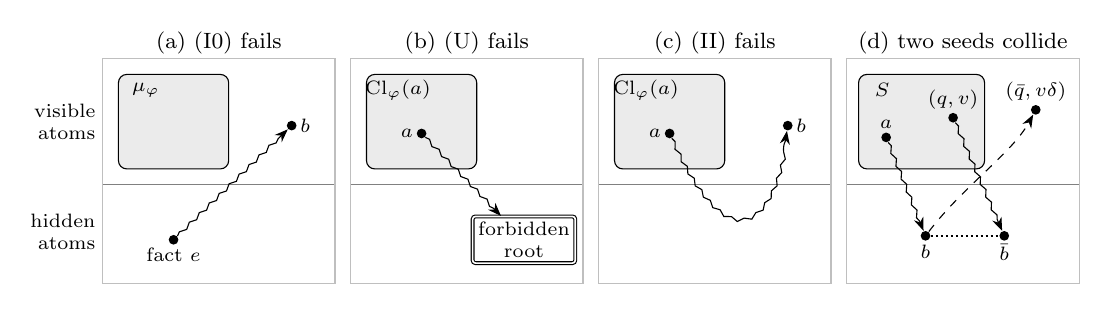
\begin{tikzpicture}[>=Stealth,font=\small,x=1cm,y=1cm,
    every node/.style={inner sep=1.5pt},
    model/.style={draw,rounded corners=3pt,fill=black!8},
    pt/.style={circle,fill,inner sep=0pt,minimum size=3.5pt},
    der/.style={->,decorate,decoration={snake,amplitude=0.6pt,segment length=5pt,post length=3pt}},
    dual/.style={->,dashed},
    opp/.style={densely dotted,thick},
    lb/.style={font=\scriptsize,inner sep=1pt},
    ttl/.style={font=\footnotesize,anchor=south}]
  \foreach \k in {0,1,2,3} {
    \begin{scope}[xshift=3.15*\k cm]
      \draw[black!50] (0,0) -- (2.95,0);
      \draw[black!25] (0,-1.25) rectangle (2.95,1.6);
    \end{scope}}
  \node[lb,anchor=east,align=right] at (-0.05,0.8) {visible\\ atoms};
  \node[lb,anchor=east,align=right] at (-0.05,-0.6) {hidden\\ atoms};
  % (a) (I0)
  \node[ttl] at (1.475,1.6) {(a) \CondI\ fails};
  \draw[model] (0.2,0.2) rectangle (1.6,1.4);
  \node[lb] at (0.55,1.2) {$\mu_\varphi$};
  \node[pt,label={[lb]below:fact $e$}] (ea) at (0.9,-0.7) {};
  \node[pt,label={[lb]right:$b$}] (ba) at (2.4,0.75) {};
  \draw[der] (ea) -- (ba);
  % (b) (U)
  \begin{scope}[xshift=3.15cm]
    \node[ttl] at (1.475,1.6) {(b) \CondU\ fails};
    \draw[model] (0.2,0.2) rectangle (1.6,1.4);
    \node[lb] at (0.6,1.2) {$\Cl_\varphi(a)$};
    \node[pt,label={[lb]left:$a$}] (ab) at (0.9,0.65) {};
    \node[draw,double,rounded corners=1pt,lb,inner sep=2pt,align=center] (fb) at (2.2,-0.7) {forbidden\\ root};
    \draw[der] (ab) -- (fb);
  \end{scope}
  % (c) (II)
  \begin{scope}[xshift=6.3cm]
    \node[ttl] at (1.475,1.6) {(c) \CondII\ fails};
    \draw[model] (0.2,0.2) rectangle (1.6,1.4);
    \node[lb] at (0.6,1.2) {$\Cl_\varphi(a)$};
    \node[pt,label={[lb]left:$a$}] (ac) at (0.9,0.65) {};
    \node[pt,label={[lb]right:$b$}] (bc) at (2.4,0.75) {};
    \draw[der] (ac) .. controls (1.6,-0.9) and (2.2,-0.6) .. (bc);
  \end{scope}
  % (d) collision
  \begin{scope}[xshift=9.45cm]
    \node[ttl] at (1.475,1.6) {(d) two seeds collide};
    \draw[model] (0.15,0.2) rectangle (1.75,1.4);
    \node[lb] at (0.45,1.2) {$S$};
    \node[pt,label={[lb]above:$a$}] (ad) at (0.5,0.6) {};
    \node[pt,label={[lb]above:$(q,v)$}] (qd) at (1.35,0.85) {};
    \node[pt,label={[lb]below:$b$}] (bd) at (1.0,-0.65) {};
    \node[pt,label={[lb]below:$\bar b$}] (nbd) at (2.0,-0.65) {};
    \node[pt,label={[lb]above:$(\bar q,v\delta)$}] (rd) at (2.4,0.95) {};
    \draw[der] (ad) -- (bd);
    \draw[der] (qd) -- (nbd);
    \draw[opp] (bd) -- (nbd);
    \draw[dual] (bd) .. controls (1.5,0.0) and (2.1,0.4) .. (rd);
  \end{scope}
\end{tikzpicture}
\caption{When both systems are satisfiable, the four ways in which a model $S$
of $\varphi$ can fail to extend to a model of $\psi$, in the proof of
\cref{thm:ch-characterization}. Upper halves
hold visible atoms, lower halves hidden ones; wavy arrows are derivations of
$\psi$, and the shaded box is a model of $\varphi$. (a) A fact of $\psi$
derives a visible atom outside the least model $\mu_\varphi$. (b) A seed $a$
derives a forbidden root; then the least model $\Cl_\varphi(a)$ of $\varphi$
that contains $a$ cannot be extended. (c) A seed $a$ derives a visible atom
outside $\Cl_\varphi(a)$. (d) Two seeds of $S$ derive opposite atoms $b$ and
$\bar b$, possibly hidden. Collision return (\cref{lem:lf-collision}) reverses
the second derivation by duality (dashed): the single seed $a$ derives the
opposite of the extension $(q,v\delta)\in S$ of the second seed, an atom
outside $S\supseteq\Cl_\varphi(a)$, so this is case~(c). If $a$ is a fact of
$\psi$ instead, it is case~(a).}
\Description{Four panels, each split by a horizontal line into visible atoms
above and hidden atoms below. In each panel a shaded box is a model of phi.
Panel a: a fact e of psi, below the line, derives by a wavy arrow a visible
atom b outside the box labeled mu phi. Panel b: a seed a inside the box,
labeled closure of a, derives a doubly framed forbidden root below the line.
Panel c: a seed a inside the box derives, through hidden atoms, a visible atom
b outside the box. Panel d: two seeds a and q v inside the box labeled S
derive the hidden atoms b and b bar, joined by a dotted line; a dashed arrow from b
leads to the visible atom q bar, v delta outside the box.}
\label{fig:ch-conditions}
\end{figure}


\begin{proof}
Item (1) is immediate from \cref{def:bg-existential}.

For (2), assume that $\varphi$ and $\psi$ are satisfiable. We first show
that the three conditions are necessary. Assume $\varphi\models\Exists\psi$.
The least model $\mu_\varphi$ of $\varphi$ is $T|_X$ for some model $T$ of
$\psi$ by \cref{eq:ch-models}, and $T\supseteq\mu_\psi$ by
\cref{lem:lf-closure}(2); hence $\mu_\psi|_X\subseteq T|_X=\mu_\varphi$,
which is \CondI. Let $a$ be a visible atom that is live in $\varphi$. Its
least model $\Cl_\varphi(a)$ is $T|_X$ for a model $T$ of $\psi$. Since $T$
contains $a$ and is closed under the rules of $\psi$, it contains $\Reach_\psi(a)$.
As $T$ contains no forbidden root, this gives \CondU, and
$\Reach_\psi(a)|_X\subseteq T|_X=\Cl_\varphi(a)$ gives \CondII.

Conversely, assume \CondI, \CondU\ and \CondII, let $S$ be a model of
$\varphi$, and put $T=H_\psi(S)$, where $S$ is read as a set of atoms over
$X\cup Z$. By \cref{lem:lf-closure}(5) and \cref{eq:ch-models}, it suffices
to show that $T|_X=S$ and that $T$ is consistent. Every atom of $S$ is live
in $\varphi$, and $\Cl_\varphi(a)\subseteq S$ for every $a\in S$ by
\cref{lem:lf-closure}(1), since $S$ is closed under the rules of $\varphi$ and
contains its facts.

\emph{Visible part.} Clearly $S\subseteq T|_X$. A visible atom of $T$ lies in
$\mu_\psi|_X\subseteq\mu_\varphi\subseteq S$, by \CondI, or in $\Reach_\psi(a)|_X$
for some $a\in S$, which lies in $\Cl_\varphi(a)\subseteq S$ by \CondII.

\emph{Consistency.} Suppose that $T$ is not consistent, and take seeds
$x,y\in\Fact_\psi\cup S$ as in \cref{lem:lf-closure}(3). If $\Reach_\psi(x)$
contains a forbidden root, then $x\notin\Fact_\psi$, because $\mu_\psi$ is
consistent; so $x\in S$, contradicting \CondU. Otherwise $b\in \Reach_\psi(x)$
and $\bar b\in \Reach_\psi(y)$ for some atom $b$; since an exclusion pair is
unordered, we may assume that $y\in S$ if one of $x,y$ lies in $S$.
\begin{itemize}[leftmargin=*]
\item If $x,y\in\Fact_\psi$, then $b,\bar b\in\mu_\psi$, contradicting the
  consistency of $\mu_\psi$.
\item If $x\in\Fact_\psi$ and $y=(q,v)\in S$, then \cref{lem:lf-collision}
  gives $(\bar q,v\delta)\in \Reach_\psi(x)\subseteq\mu_\psi$ for some $\delta$.
  This atom is visible, so it lies in $\mu_\varphi\subseteq S$ by \CondI. But
  $(q,v\delta)\in S$ because $S$ is extension closed, and $S$ has an
  exclusion pair.
\item If $x\in S$ and $y=(q,v)\in S$, possibly $x=y$, then
  \cref{lem:lf-collision} gives $(\bar q,v\delta)\in \Reach_\psi(x)|_X$ for some
  $\delta$, which lies in $\Cl_\varphi(x)\subseteq S$ by \CondII. Again
  $(q,v\delta)\in S$, and $S$ has an exclusion pair.
\end{itemize}
Each case contradicts an assumption. Hence $T$ is a model of $\psi$ with
$T|_X=S$, so $S\in\mathcal F_\psi$.
\end{proof}

The proof shows that, when the conditions hold, $H_\psi(S)$ is the least
extension of every model $S$ of $\varphi$; when a condition fails, the least
model $\mu_\varphi$ or $\Cl_\varphi(a)$ that refutes it is a countermodel.
The two qualifications of the theorem are needed.
\begin{itemize}[leftmargin=*]
\item \emph{The satisfiability dispatch.} Let $X=\{x\}$, $\varphi$ empty, and
  $\psi=\{z=\Bot,\ \Top\le z\}$ with $z$ hidden. Then $\mu_\psi$ consists of
  atoms of $z$, and $\psi$ has no rule that involves $x$ other than its
  extensions, so the three conditions hold; but $\psi$ is unsatisfiable, and
  the entailment fails.
\item \emph{Condition \CondU.} Let $n\ge0$, $X=\{y\}$, $\varphi$ empty, and
  $\psi=\{y\le f(z_i)_i\}$ with distinct hidden variables $z_i$. Then $\psi$
  has no facts, and its only pure moves from visible atoms are the
  pops $(y^0,iw)\to(z_i^{c(i)},w)$, after which no pure move applies. By
  \cref{lem:ch-pure} below, \CondI\ and \CondII\ hold. But $y=\Top$ has no
  extension: \CondU\ fails at the live atom $(y^0,\eps)$, which is a
  forbidden root of $\psi$.
\end{itemize}
The theorem also depends on duality. For a set of one-premise rules without
duals, say $(x^0,w)\to(z^0,w)$ and $(y^0,w)\to(z^1,w)$ with $z$ hidden, the
three conditions hold for the empty antecedent, but $x=y=\Top$ produces an
exclusion pair at $z$. No system has exactly these rules: by
\cref{lem:lf-duality}, a system with these rules also has the duals
$(z^1,w)\to(x^1,w)$ and $(z^0,w)\to(y^1,w)$, which expose the collision as the
visible consequences $(x^0,w)\Rightarrow^*(y^1,w)$ and
$(y^0,w)\Rightarrow^*(x^1,w)$, and \CondII\ fails.

The conditions only need pure derivations of $\psi$, from extended seeds.

\begin{lemma}[Pure forms]\label{lem:ch-pure}
\leavevmode
\begin{enumerate}[leftmargin=*]
\item \CondU\ holds iff there are no visible atom $(p,u)$ that is live in
  $\varphi$, word $\alpha$ and forbidden root $e$ of $\psi$ with
  $(p,u\alpha)\to^*_\psi e$.
\item \CondII\ holds iff $b\in\Cl_\varphi(p,u)$ for every visible atom
  $(p,u)$ that is live in $\varphi$ and every visible atom $b$ with
  $(p,u)\to^*_\psi b$.
\end{enumerate}
\end{lemma}

\begin{proof}
If $(p,u)$ is live in $\varphi$, so is $(p,u\alpha)$, and
$\Cl_\varphi(p,u\alpha)\subseteq\Cl_\varphi(p,u)$
(\cref{lem:lf-closure}(4)). By \cref{lem:lf-ext-first}, $b\in \Reach_\psi(p,u)$
iff $(p,u\alpha)\to^*_\psi b$ for some $\alpha$. Item (1) follows directly,
since $(p,u\alpha)$ is again a live visible atom. For (2), the condition is
clearly necessary. Conversely, if $b\in \Reach_\psi(p,u)|_X$ for a live $(p,u)$,
then $(p,u\alpha)\to^*_\psi b$ for some $\alpha$, and the condition, applied
to the live atom $(p,u\alpha)$, gives
$b\in\Cl_\varphi(p,u\alpha)\subseteq\Cl_\varphi(p,u)$.
\end{proof}

\begin{example}[The consequent $x\le z\to z$]\label{ex:ch-arrow}
For the arrow of \cref{ex:lf-arrow}, let $X=\{x\}$, $Z=\{z\}$ and
$\psi=\{x\le z\to z\}$, the literal $x\le f(z,z)$. By
\cref{tab:lf-clauses}, $\psi$ has the forbidden root $(x^0,\eps)$, no
facts, and the pure moves
\[
 (x^0,0w)\to(z^1,w)\to(x^1,1w),\qquad (x^0,1w)\to(z^0,w)\to(x^1,0w).
\]
No pure move leaves a negative atom of $x$. So the pure derivations of $\psi$
of positive length between visible atoms are exactly
$(x^0,iw)\to^*(x^1,\bar\imath w)$, where $\bar\imath=1-i$: $\psi$ exchanges
the first letter and the sign. Since $\mu_\psi=\varnothing$, \CondI\ holds for
every antecedent, and $\psi$ is satisfiable, with $x=\Bot$.

\emph{The empty antecedent.} Let $\varphi_0$ be empty. Then \CondU\ fails at
$(x^0,\eps)$, with the countermodel $x=\Top$. Condition \CondII\ fails at
$(x^0,0)$: $\psi$ derives $(x^1,1)$, but $\Cl_{\varphi_0}((x^0,0))$ consists of
the atoms $(x^0,0w)$, the leaf pair $(0\Sigma^*,\varnothing)$ of the
countermodel $x=\Bot\to\Omega$ (\cref{ex:lf-arrow}). Indeed
$\Bot\to\Omega\le_c z\to z$ would require $z\le_c\Bot$ and $\Omega\le_c z$.
The tree $\Bot\to\Top$, with leaf pair $(\Sigma^+,\varnothing)$, fails for a
reason that a priori involves two seeds: the closures of $(x^0,0)$ and
$(x^0,1)$ under $\psi$ contain the exclusion pair $(z^1,\eps)$ and
$(z^0,\eps)$. Collision return reverses the second branch
$(x^0,1)\to(z^0,\eps)$ into $(z^1,\eps)\to(x^1,1)$, which continues the first
branch: the single seed $(x^0,0)$ derives $(x^1,1)$, the opposite of the
second seed, and \CondII\ fails at $(x^0,0)$. The extension in
\cref{lem:lf-collision} is needed in general. The atom $(x^0,\eps)$ derives
$(z^0,\eps)$ through its extension $(x^0,1)$, which collides with the atom
$(z^1,\eps)$ derived from $(x^0,0)$; collision return gives $(x^1,1)$, the
opposite of an extension of $(x^0,\eps)$, whereas $(x^1,\eps)$ is not
derivable from $(x^0,0)$.

\emph{The antecedent $x\le x\to x$.} Let $\varphi_1=\{x\le x\to x\}$ be the
system of \cref{ex:lf-clauses}. It is satisfiable. Condition \CondU\ holds,
because $(x^0,\eps)$ is a forbidden root of $\varphi_1$ as well, hence dead.
For \CondII, by \cref{lem:ch-pure} it suffices that
$(x^1,\bar\imath w)\in\Cl_{\varphi_1}((x^0,iw))$ for every live $(x^0,iw)$,
and $\varphi_1$ derives it: $(x^0,0w)\to(x^1,w)\to(x^1,1w)$ by $\mathrm{pop}_0$ and
$\mathrm{push}_1$, and $(x^0,1w)\to(x^0,w)\to(x^1,0w)$ by $\mathrm{pop}_1$
and $\mathrm{push}_0$. By \cref{thm:ch-characterization},
$\varphi_1\models\exists z\,\psi$; indeed $z=x$ is a witness.
\end{example}

\subsection{Special Cases}\label{sec:ch-remarks}

\begin{remark}[Covariant and joint-parity instances]\label{rem:ch-parity}
A \emph{parity assignment} of a system $\chi$ is a map $\pi:V\to\{0,1\}$ with
$\pi(u)=\pi(v)$ for every literal $u\le v$ and $\pi(a_i)=\pi(u)\oplus c(i)$
for every $i$ and every literal $f(a_i)_i\le u$ or $u\le f(a_i)_i$ of $\chi$.
By \cref{tab:lf-clauses}, every rule of $\chi$ then preserves the bit
$\kappa(v^s,w)=s\oplus\pi(v)$ of an atom; for instance, $\mathrm{push}_i$ of
$f(a_i)_i\le u$ leads from $\kappa=c(i)\oplus\pi(a_i)=\pi(u)$ to
$\kappa=\pi(u)$. Opposite atoms have different bits. Hence no derivation
leads from an atom to the opposite of one of its extensions: self-collisions,
cause (c) of \cref{cor:lf-dead}, do not occur, and in a satisfiable system
every dead atom is dead by support. Likewise, in \cref{lem:lf-collision}
the two colliding seeds have different bits, so in the proof of
\cref{thm:ch-characterization} two branches from the same seed never collide.

More is true. Rename every atom $(v^s,w)$ to $(v^{s\oplus\pi(v)},w)$. By
\cref{tab:lf-clauses}, this maps the rules, facts and forbidden
roots of $\chi$ onto those of the following system $\chi^\pi$ for the
covariant variance $c=0$: $\chi^\pi$ keeps every literal of $\chi$ whose root
has $\pi=0$ and reverses every other one, where the root of $u\le v$, $u=\Bot$
and $\Top\le u$ is $u$. Reversal turns $u\le v$ into $v\le u$, a lower
constructor literal into the upper one with the same variables and
conversely, and exchanges $u=\Bot$ and $\Top\le u$. On trees the renaming is
$\rho(v)\mapsto\nu_{\pi(v)}\rho(v)$, read covariantly: the covariant leaf
cone of sign $s\oplus\pi(v)$ of $\nu_{\pi(v)}\rho(v)$ is the cone $L^s$ of
$\rho(v)$, because $(\nu_rt)^\partial=\nu_{1\oplus r}t$ by
\cref{lem:bg-normalization}(1). So $\rho$ solves
$\chi$ iff this assignment solves $\chi^\pi$, by \cref{lem:lf-clauses}. If
$\varphi\wedge\psi$ has a \emph{joint} parity assignment, one renaming serves
both systems and keeps visibility, and the instance is equivalent to a
covariant instance of the same size, in every tree class, since $\nu_r$ is an
involution that preserves finiteness and regularity
(\cref{lem:bg-normalization}). The covariant case itself is $\pi=0$, where
every rule keeps the sign and the rules of sign $1$ are the duals of the
rules of sign $0$.

\Cref{thm:ch-characterization} needs no parity assignment, and the system
$x\le x\to x$ has none, since it would require $\pi(x)=\pi(x)\oplus c(0)$. Its
self-collision $(x^0,00)\to(x^1,0)$ (\cref{ex:lf-least}) is exactly what a
parity assignment excludes.
\end{remark}

\begin{remark}[One sign: the signature $\BF$]\label{rem:ch-one-sign}
Let $f$ be covariant, and consider trees over $\BF$ and systems without
literals $\Top\le u$ (\cref{sec:bg-trees}). Every leaf of such a tree has
sign $1$, so $L^0_t=\varnothing$, and $L^1_t$ is the complement of the set
$\Kpos(t)$ of positions labeled $f$ (\cref{thm:lf-representation}(4)). The
trees over $\BF$ thus correspond to the extension-closed sets of negative
atoms. All facts of such a system come from literals $u=\Bot$ and are
negative atoms, and every rule keeps the sign, so the closure of a set of negative atoms consists of
negative atoms, and an exclusion pair never arises. The models over $\BF$ are
therefore the sets of negative atoms that contain the facts, are
closed under the rules, and avoid the forbidden roots $(u^1,\eps)$ of the
lower constructor literals $f(a_i)_i\le u$. \Cref{lem:lf-closure} and
\cref{thm:ch-characterization} hold over $\BF$, with satisfiability over
$\BF$, by the same proofs, in which the exclusion case is void, once every
set of atoms is taken in the universe
$\Conf^-_V=\{v^1:v\in V\}\times\Sigma^*$ of negative atoms: the seed sets,
the visible sets, the models, the closures, liveness, and the atoms
quantified in the three conditions are all negative. (Without this
restriction the statement fails: for the empty system the closure of
$(x^0,\eps)$ is consistent, but no $\Top$-free assignment contains it.)

Read through complements, a negative atom $(v^1,w)$ says $w\notin\Kpos(v)$,
and each rule on negative atoms is the contrapositive of a clause on
constructor positions: $u\le v$ says $\Kpos(u)\subseteq\Kpos(v)$,
$f(a_i)_i\le u$ says $\eps\in\Kpos(u)$ and $i\Kpos(a_i)\subseteq\Kpos(u)$,
$u\le f(a_i)_i$ says that $iw\in\Kpos(u)$ implies $w\in\Kpos(a_i)$, $u=\Bot$
says $\eps\notin\Kpos(u)$, and extensions say that $\Kpos(v)$ is prefix closed.
In these terms, \CondI\ says that every visible position that some solution
of $\varphi$ puts into a variable is put there by some solution of $\psi$;
\CondU\ says that every visible position that every solution of $\psi$ puts
into a variable is put there by every solution of $\varphi$; and \CondII,
read contrapositively, says that every solution of $\varphi$ is closed under
the visible consequences of the clauses of $\psi$. Over $\BF$ the three
conditions therefore compare, respectively, the unions of all solutions, the
least solutions, and the closures of single positions, for $\varphi$ and for
the projection of $\psi$. In this picture the solution sets are closed under
nonempty unions and intersections of constructor positions, no exclusions
and no self-collisions occur, and the only obstructions are single seeds. The
decision procedure of this paper does not treat $\BF$ separately; it reduces
$\BF$ to $\BFT$ (\cref{sec:tc}).
\end{remark}

A forbidden root has the empty word, so the pure derivations in
\cref{lem:ch-pure}(1) end with an empty stack. A failure of \CondII\ with a
live seed $a$ and a consequence $b$ is thus witnessed by a pure derivation of
$\psi$ from a live extension of $a$ to $b$, with $b$ outside the least model
of $\varphi$ that contains that extension. \Cref{sec:sm,sec:un,sec:ex} turn the satisfiability tests, \CondI,
\CondU\ and this form of \CondII\ into problems about finite automata.

%% classes -- tree classes: two seeds, observation pins, finite-bound pinning
%% for every variance, regular and finite transfer, the top-freeness gadget
%% for {bot,f}, and arities zero and one.

\section{Tree Classes}\label{sec:tc}\label{sec:classes}

The preceding sections decide existential entailment over arbitrary trees.
This section transfers the decision to regular and to finite trees, for every
arity $n\ge0$ and every variance $c$, and it reduces the signature $\BF$ with
$f$ covariant to $\BFT$. Regular trees are handled by the least closures of
\cref{sec:lf}, whose slices are regular for regular seeds by
\cref{lem:sm-regular-closure}; a failed extension is caused by at most two
seeds (\cref{lem:tc-two-seeds}), so $\Ereg=\Eall$ (\cref{thm:tc-regular}).
Finite trees need a different argument. Least closures describe trees with as
few leaves as possible, and these are infinite in general: the empty system has the empty least model, which
assigns $\Omega$ to every variable. Instead we express observations by finite
ground bounds (\cref{lem:tc-pins}) and show that adding finite ground bounds
preserves finite satisfiability, for every variance (\cref{thm:tc-pinning}).
This gives the dispatch \cref{eq:tc-finite} of \cref{thm:tc-finite}. Proofs
not given here are in \cref{app:tc}.

Throughout, trees are over $\BFT$ and ordered by $\le_c$ unless stated
otherwise, $\varphi$ and $\psi$ are as in \cref{def:bg-existential}, we use
the notation of \cref{sec:bg,sec:lf} together with $f(t^n)=f(t,\dots,t)$ and
$\nu_\pm$ for $\nu_0$ and $\nu_1$, and a model $T$ \emph{decodes} to the
solution $\rho$ with $S_\rho=T$ (\cref{lem:lf-clauses}).

\subsection{Extensions and Two Seeds}\label{sec:tc-seeds}

An assignment $\rho$ of $X$ is \emph{extensible} if it extends to a solution
of $\psi$ over arbitrary trees.

\begin{lemma}[Extension criterion]\label{lem:tc-extension}
An assignment $\rho$ of $X$ is extensible iff $H_\psi(S_\rho)$ is consistent
and $H_\psi(S_\rho)|_X=S_\rho$. In that case $H_\psi(S_\rho)$ decodes to an
extension of $\rho$.
\end{lemma}

This restates \cref{lem:lf-closure}(5) for assignments.

\begin{proof}
By \cref{lem:lf-closure}(5) and \cref{lem:lf-clauses}, applied to the set
$S_\rho$, which is extension closed and has no exclusion pair, $\rho$ is
extensible exactly when $H_\psi(S_\rho)$ is consistent and has visible part
$S_\rho$; then that closure decodes to an extension.
\end{proof}

\begin{definition}[Observations]\label{def:tc-observation}
A \emph{visible observation} is a visible atom $a=(x^\pm,w)$ together with one
of the words \emph{asserted} or \emph{denied}. An asserted observation
\emph{holds} in an assignment $\rho$ of $X$ if $a\in S_\rho$, a denied one if
$a\notin S_\rho$. The variable $x$ and the word $w$ are the variable and the
word of the observation.
\end{definition}

\begin{lemma}[Two seeds]\label{lem:tc-two-seeds}
Let $\rho$ be an assignment of $X$ that is not extensible. There are a set
$A\subseteq S_\rho$ of visible atoms and a set $C$ of visible atoms outside
$S_\rho$, with $\len A+\len C\le2$, such that no assignment $\rho'$ of $X$
with $A\subseteq S_{\rho'}$ and $C\cap S_{\rho'}=\varnothing$ is extensible.
In particular, at most two visible observations hold in $\rho$ and hold
together in no extensible assignment.
\end{lemma}

\begin{proof}
Every atom $b$ of $H_\psi(S_\rho)$ has a seed in $\Fact_\psi\cup S_\rho$, so
$b\in H_\psi(A_b)$ for a set $A_b\subseteq S_\rho$ with at most one element. By
\cref{lem:tc-extension}, $H_\psi(S_\rho)$ is not consistent or has a visible
atom outside $S_\rho$. In the first case, \cref{lem:lf-closure}(3) gives
seeds $x,y\in\Fact_\psi\cup S_\rho$ such that $\Reach_\psi(x)$ contains a
forbidden root, or $\Reach_\psi(x)$ and $\Reach_\psi(y)$ contain an exclusion pair;
let $A$ consist of those of $x,y$ that lie in $S_\rho$, and $C=\varnothing$.
In the second case, let $b\in H_\psi(S_\rho)|_X$ with $b\notin S_\rho$, and put
$A=A_b$ and $C=\{b\}$. In both cases $\len A+\len C\le2$. Let $\rho'$ be an
assignment of $X$ with $A\subseteq S_{\rho'}$ and $C\cap
S_{\rho'}=\varnothing$. Since $H_\psi$ is monotone,
$H_\psi(S_{\rho'})\supseteq H_\psi(A)$, so $H_\psi(S_{\rho'})$ contains the
same forbidden root or the same two opposite atoms, or the visible atom
$b\notin S_{\rho'}$. By \cref{lem:tc-extension}, $\rho'$ is not extensible.
The observations asserting the atoms of $A$ and denying those of $C$ prove the
last claim.
\end{proof}

The lemma uses no satisfiability hypothesis. If $\psi$ is unsatisfiable, then
$\mu_\psi$ is inconsistent by \cref{lem:lf-closure}(2), and
$A=C=\varnothing$ will do. The two seeds of $A$ may belong to the same
variable.

\subsection{Observation Pins}\label{sec:tc-pins}

For a word $w$ and trees $b,g$, let $\emb_b(w,g)$ be the tree with a pin path
along $w$ that carries $g$ at its end and $b$ at every child off the pin path:
$\emb_b(\eps,g)=g$, and $\emb_b(iw,g)=f(t_j)_j$ with $t_i=\emb_b(w,g)$ and
$t_j=b$ for $j\ne i$.

\begin{lemma}[Observation pins]\label{lem:tc-pins}
For every covariant tree $t$ and every word $w$,
\begin{equation}\label{eq:tc-pins}
\begin{aligned}
 w\in L^0_t&\iff\emb_\Bot(w,\Top)\le t,&
 w\notin L^0_t&\iff t\le\emb_\Top(w,f(\Top^n)),\\
 w\in L^1_t&\iff t\le\emb_\Top(w,\Bot),&
 w\notin L^1_t&\iff\emb_\Bot(w,f(\Bot^n))\le t,
\end{aligned}
\end{equation}
and each of these four trees has at most $1+n(\len w+1)$ positions.
Consequently, for every variance $c$, every visible observation with variable
$x$ and word $w$ is equivalent, for all assignments $\rho$ of $X$, to a single
inequality $g\le_c\rho(x)$ or $\rho(x)\le_cg$, where $g$ is a finite ground
tree with at most $1+n(\len w+1)$ positions.
\end{lemma}

For $n\ge1$ the bound is attained by the two trees with a constructor at the
end of the pin path; for $n=0$ the only word is $\eps$, and the four trees are
$\Top$, $f()$, $\Bot$ and $f()$.

\subsection{Finite-Bound Pinning}\label{sec:tc-pinning}

\paragraph{Intersection of leaf cones}
Over arbitrary and regular trees, extensions can be intersected; over finite
trees they cannot (item (3) below), which is why the transfer to finite trees
pins observations by finite ground bounds instead. For trees $t$ and $u$, let
$t\leafmeet u$ be the tree with the leaf pair
$(L^0_t\cap L^0_u,\ L^1_t\cap L^1_u)$, which exists by
\cref{thm:lf-representation}(1); its signed leaf cones contain exactly the
observations common to $t$ and $u$. For assignments, $\leafmeet$ acts variablewise.

\begin{proposition}[Closure under intersection]\label{prop:ch-meet}
\leavevmode
\begin{enumerate}[leftmargin=*]
\item The intersection of a nonempty family of models of a system $\chi$ is a
  model of $\chi$, and the intersection of a nonempty subfamily of the
  projected family $\mathcal F_\psi$ (\cref{eq:ch-models}) belongs to
  $\mathcal F_\psi$. In particular, the solutions of $\chi$ and the assignments of $X$ that extend
  to solutions of $\psi$ are closed under $\leafmeet$.
\item The operation $\leafmeet$ is commutative, associative, idempotent and
  monotone for $\le_c$, and
  $f(t_i)_i\leafmeet f(u_i)_i=f(t_i\leafmeet u_i)_i$. Moreover,
  $t\leafmeet u$ is the median of $t$, $u$ and $\Omega$ in the lattice of
  trees ordered by $\le_c$.
\item If $t$ and $u$ are regular, then so is $t\leafmeet u$. For $n\ge1$,
  $\Bot\leafmeet\Top=\Omega$ is infinite, so the finite trees are not
  closed under $\leafmeet$.
\end{enumerate}
\end{proposition}

The proof is in \cref{app:tc}. By (1), the model $H_\psi(S)$ of
\cref{lem:lf-closure}(5) is the intersection of all models $T$ of $\psi$ with
$T|_X=S$, the least extension of $S$. By (1) and commutativity, a relation
that is the projection of the solutions of a system over arbitrary trees, or
over regular trees, and contains two pairs $(a,b)$ and $(b,a)$ also contains
the diagonal pair $(a\leafmeet b,a\leafmeet b)$. So no such relation is
nonempty, symmetric and irreflexive; in particular, over arbitrary or regular
trees no system with hidden variables defines the disequality of two trees.
The decision procedure does not use \cref{prop:ch-meet}.

\paragraph{Ground bounds}
A \emph{ground bound} on a variable $x$ is an inequality $g\le_cx$, a
\emph{lower} bound, or $x\le_cg$, an \emph{upper} bound, where $g$ is a finite
ground tree. The following theorem extends
\nssecite{Theorem ``Finite countermodel transfer''} from the pin paths of a
single word to arbitrary finite bounds.

\begin{theorem}[Finite-bound pinning]\label{thm:tc-pinning}
Let $\chi$ be a system over a set $V$ of variables, with any variance, that
has a finite solution, and let $B$ be a finite set of ground bounds on
variables of $V$. If $\chi\cup B$ has a solution, then it has a finite
solution.
\end{theorem}

The proof reduces the theorem to covariant systems by the signed system
$\chi^\pm$ of \cref{tab:bg-signed}, and then symmetrizes a covariant solution
by a median. A ground bound $b$ is translated into a pair $b^\pm$ of
covariant ground bounds on signed variables,
\begin{equation}\label{eq:tc-signed-bounds}
 (g\le_cx)^\pm=\{\nu_+g\le x^+,\ x^-\le\nu_-g\},\qquad
 (x\le_cg)^\pm=\{x^+\le\nu_+g,\ \nu_-g\le x^-\},
\end{equation}
and $B^\pm$ is the union of these pairs. For an assignment $\rho$ of $V$,
$\rho^\pm$ is the assignment $v^\pm\mapsto\nu_\pm\rho(v)$ of
\cref{lem:bg-signed}. The \emph{sign involution} $\iota$ maps an assignment
$\sigma$ of $V^\pm$ to the assignment
\[
 (\iota\sigma)(v^+)=\sigma(v^-)^\partial,\qquad
 (\iota\sigma)(v^-)=\sigma(v^+)^\partial .
\]
The literals of \cref{tab:bg-signed} that contain $\Bot$ or $\Top$ belong to
$\chi^\pm$; the proof needs them (\cref{rem:tc-extreme}).

\begin{lemma}[Signed bounds]\label{lem:tc-signed}
Let $\chi$ be a system over $V$ and $B$ a finite set of ground bounds on $V$.
\begin{enumerate}[leftmargin=*]
\item An assignment $\rho$ of $V$ solves $\chi\cup B$ iff $\rho^\pm$ solves
  $\chi^\pm\cup B^\pm$.
\item $\iota$ is an involution that maps the solutions of $\chi^\pm\cup B^\pm$
  to solutions, and $\iota\rho^\pm=\rho^\pm$ for every assignment $\rho$ of
  $V$.
\item If $\iota\sigma=\sigma$, then $\sigma=\rho^\pm$ for the assignment
  $\rho(v)=\nu_+\sigma(v^+)$; and $\rho\mapsto\rho^\pm$ and its inverse
  preserve finiteness.
\end{enumerate}
\end{lemma}

For covariant trees $t_1,t_2,t_3$, the \emph{median} $\tcmed(t_1,t_2,t_3)$ is
the covariant tree whose cones consist of the words that lie in the
corresponding cones of at least two of the three trees: for both signs,
\[
 L^\pm_{\tcmed(t_1,t_2,t_3)}=\{w:w\in L^\pm_{t_j}\text{ for at least two }j\}.
\]
It exists by \cref{thm:lf-representation}(1): the sets on the right are
extension closed, and they are disjoint, since a word in two of the cones
$L^0_{t_j}$ and in two of the cones $L^1_{t_j}$ lies in both cones of one
$t_j$. The median of assignments is taken variablewise. It is the lattice
median $(t_1\wedge t_2)\vee(t_1\wedge t_3)\vee(t_2\wedge t_3)$ of the
covariant order, but we use only the following properties.

\begin{lemma}[Median]\label{lem:tc-median}
\leavevmode
\begin{enumerate}[leftmargin=*]
\item The median is symmetric and monotone in each argument, and
  $\tcmed(t,t,u)=t$.
\item $\tcmed(f(a^1_i)_i,f(a^2_i)_i,f(a^3_i)_i)=f(\tcmed(a^1_i,a^2_i,a^3_i))_i$
  and $\tcmed(t_1,t_2,t_3)^\partial=\tcmed(t_1^\partial,t_2^\partial,t_3^\partial)$.
  In particular $\iota$ commutes with medians of assignments of signed
  variables.
\item The median of three finite trees is finite.
\item If three assignments solve a covariant system together with covariant
  ground bounds, so does their median.
\end{enumerate}
\end{lemma}

The covariant case of \cref{thm:tc-pinning} is proved directly from the
finite-satisfiability criterion of \citet{Zhao26}
(\cref{thm:bg-nsse-sat}), in \cref{app:tc-covariant}. By that
criterion, a system has a finite solution iff it has neither a label clash nor
a cycle clash. The proof encodes each ground bound by fresh variables, one for
each position of the bound; since a path through fresh variables strictly
increases the length of the position they stand for, every cycle clash of the
encoded system lies among the original variables, where the finite solution
of $\chi$ excludes it, and the solution of $\chi\cup B$ excludes label
clashes.

\begin{lemma}[Covariant finite-bound pinning]\label{lem:tc-pinning-covariant}
\Cref{thm:tc-pinning} holds when $f$ is covariant.
\end{lemma}

\begin{proof}[Proof of \cref{thm:tc-pinning}]
If $n=0$, every tree is finite. Let $n\ge1$, let $\delta$ be a finite solution
of $\chi$, and let $\rho$ be a solution of $\chi\cup B$. By
\cref{lem:tc-signed}(1,3), $\delta^\pm$ is a finite solution of $\chi^\pm$,
and $\rho^\pm$ is a solution of $\chi^\pm\cup B^\pm$. By
\cref{lem:tc-pinning-covariant}, applied to the covariant system $\chi^\pm$
and the bounds $B^\pm$, the system $\chi^\pm\cup B^\pm$ has a finite solution
$\alpha$. By \cref{lem:tc-signed}(2), $\iota\alpha$ is a solution of
$\chi^\pm\cup B^\pm$, and it is finite because duality keeps the domain. Consider the
median
\[
 \tcmed(\alpha,\iota\alpha,\delta^\pm).
\]
All three arguments solve $\chi^\pm$, so $\tcmed(\alpha,\iota\alpha,\delta^\pm)$
solves $\chi^\pm$ by \cref{lem:tc-median}(4), and it is finite by
\cref{lem:tc-median}(3). The assignment $\delta^\pm$ need not satisfy the
bounds; still $\tcmed(\alpha,\iota\alpha,\delta^\pm)$ satisfies $B^\pm$: for a
lower bound $G\le p$ in $B^\pm$, both $\alpha(p)$ and $(\iota\alpha)(p)$ lie
above $G$, so
$G=\tcmed(G,G,\delta^\pm(p))\le\tcmed(\alpha,\iota\alpha,\delta^\pm)(p)$ by
\cref{lem:tc-median}(1), and upper bounds are symmetric. By
\cref{lem:tc-median}(2) and \cref{lem:tc-signed}(2),
\[
 \iota\,\tcmed(\alpha,\iota\alpha,\delta^\pm)
 =\tcmed(\iota\alpha,\iota\iota\alpha,\iota\delta^\pm)
 =\tcmed(\iota\alpha,\alpha,\delta^\pm)=\tcmed(\alpha,\iota\alpha,\delta^\pm) .
\]
By \cref{lem:tc-signed}(3), $\tcmed(\alpha,\iota\alpha,\delta^\pm)=\tau^\pm$ for
a finite assignment $\tau$ of $V$, which solves $\chi\cup B$ by \cref{lem:tc-signed}(1).
\end{proof}

\begin{remark}[The extreme literals are needed]\label{rem:tc-extreme}
The signed literals of $u=\Bot$ and $\Top\le u$ in \cref{tab:bg-signed} cannot
be dropped from $\chi^\pm$, although they contribute no rules on leaf cones,
only facts (\cref{tab:lf-clauses}). Let $n\ge1$, $\chi=\{\Top\le x\}$,
$B=\varnothing$, and $\delta(x)=\Top$. Without its extreme literals the signed
system is empty, and $\alpha(x^+)=\Bot$, $\alpha(x^-)=\Top$ is a finite
solution with $\iota\alpha=\alpha$. Then
$\tcmed(\alpha,\iota\alpha,\delta^\pm)=\alpha$, which decodes to $x=\Bot$ and
violates $\chi$. The third argument of the median must also be a finite
solution of the unpinned system: $\Omega$ in every coordinate is fixed by
$\iota$ and solves every signed system without extreme literals, but the
median with it is infinite in general.
\end{remark}

\subsection{Regular and Finite Trees}\label{sec:tc-transfer}

\begin{theorem}[Regular trees]\label{thm:tc-regular}
For every arity $n\ge0$, every variance $c$, and all systems $\varphi$ over
$X$ and $\psi$ over $X\cup Z$:
\begin{enumerate}[leftmargin=*]
\item a system is satisfiable iff it has a regular solution;
\item every regular extensible assignment of $X$ has a regular extension;
\item if some solution of $\varphi$ is not extensible, then some regular
  solution of $\varphi$ is not extensible.
\end{enumerate}
Consequently $\Ereg(\varphi,\psi)\iff\Eall(\varphi,\psi)$.
\end{theorem}

\begin{proof}
(1) This restates \cref{thm:bg-nsse}(1) and \cref{lem:bg-signed-sat}.

(2) Let $\rho$ be regular and extensible. By \cref{lem:tc-extension},
$H_\psi(S_\rho)$ decodes to an extension of $\rho$. The cones of $\rho$ are
regular by \cref{thm:lf-representation}(4), hence so are those of
$H_\psi(S_\rho)$ by \cref{lem:sm-regular-closure}, and the extension is
regular by \cref{thm:lf-representation}(4).

(3) Let $\rho$ be a solution of $\varphi$ that is not extensible, and take $A$
and $C$ from \cref{lem:tc-two-seeds}. The model $S_\rho$ of $\varphi$ contains
$A$, so by \cref{lem:lf-closure}(2) the set $H_\varphi(A)$ is the least model
of $\varphi$ that contains $A$, and $H_\varphi(A)\subseteq S_\rho$. It decodes
to a solution $\rho_0$ of $\varphi$, which is regular by
\cref{lem:sm-regular-closure} and \cref{thm:lf-representation}(4), since $A$
is finite. Its atom set contains
$A$ and, being contained in $S_\rho$, is disjoint from $C$. By
\cref{lem:tc-two-seeds}, $\rho_0$ is not extensible.

For the consequence, if $\Eall$ holds, every regular solution of $\varphi$ is
extensible and has a regular extension by (2); if $\Eall$ fails, (3) gives a
regular solution of $\varphi$ without any extension.
\end{proof}

\begin{theorem}[Finite trees]\label{thm:tc-finite}
For every arity $n\ge0$, every variance $c$, and all systems $\varphi$ over
$X$ and $\psi$ over $X\cup Z$,
\begin{equation}\label{eq:tc-finite}
 \Efin(\varphi,\psi)\iff
 \neg\Sat_{\mathrm{fin}}(\varphi)\ \lor\
 \bigl(\Sat_{\mathrm{fin}}(\psi)\land\Eall(\varphi,\psi)\bigr).
\end{equation}
More precisely:
\begin{enumerate}[leftmargin=*]
\item if $\varphi$ has a finite solution and some solution of $\varphi$ is
  not extensible, then some finite solution of $\varphi$ is not extensible;
\item if $\psi$ has a finite solution, then every finite extensible assignment
  of $X$ has a finite extension.
\end{enumerate}
\end{theorem}

\begin{proof}
(1) Let $\rho$ be a solution of $\varphi$ that is not extensible. By
\cref{lem:tc-two-seeds}, at most two visible observations hold in $\rho$ and
hold together in no extensible assignment. By \cref{lem:tc-pins}, each of them
is equivalent to a ground bound on a visible variable; let $B$ be the set of
these bounds. Then $\rho$ solves $\varphi\cup B$, and $\varphi$ has a finite
solution, so \cref{thm:tc-pinning} gives a finite solution $\rho_1$ of
$\varphi\cup B$. The observations hold in $\rho_1$, so $\rho_1$ is not
extensible.

(2) Let $\rho$ be a finite assignment of $X$ with an extension $\rho'$ that
solves $\psi$. Let $B$ consist of the bounds $\rho(x)\le_cx$ and
$x\le_c\rho(x)$ for $x\in X$. Then $\rho'$ solves $\psi\cup B$, and $\psi$ has
a finite solution, so \cref{thm:tc-pinning} gives a finite solution $\tau$ of
$\psi\cup B$. By antisymmetry of $\le_c$, $\tau$ agrees with $\rho$ on $X$, so
it is a finite extension of $\rho$.

For \cref{eq:tc-finite}: if $\varphi$ has no finite solution, both sides
hold. If $\varphi$ has a finite solution and $\psi$ has none, that solution
has no finite extension, and both sides fail. If both have finite solutions,
(1) and (2) give $\Efin(\varphi,\psi)\iff\Eall(\varphi,\psi)$.
\end{proof}

The bounds in the proof of (1) concern at most two visible variables, and each
has at most $1+n(\len w+1)$ positions, where $w$ is the word of its
observation. The proofs of \cref{thm:tc-regular,thm:tc-finite} use no
satisfiability hypothesis and no condition on the variance.

\begin{corollary}[Decisions for regular and finite trees]\label{cor:tc-decidable}
For fixed $n$ and $c$, if existential entailment over $\BFT$ is decidable over
arbitrary trees, then it is decidable over regular trees and over finite
trees: $\Ereg=\Eall$, and $\Efin$ is decided by \cref{eq:tc-finite}, whose
two finite-satisfiability tests are decidable by \cref{thm:bg-nsse}(1).
\end{corollary}

\begin{remark}[Both finite-satisfiability tests are needed]\label{rem:tc-examples}
Let $n\ge1$ and let $c$ be any variance. For $X=\varnothing$, the empty
antecedent and $\psi=\{z\le f(z^n),\ f(z^n)\le z\}$, the entailment holds over
arbitrary and regular trees, with the unique witness $z=\Omega$, but fails
over finite trees, since $\psi$ has no finite solution. For
$\varphi=\{x\le f(x^n),\ f(x^n)\le x\}$ and $\psi=\{x=\Bot\}$, the entailment
fails over arbitrary and regular trees, at $x=\Omega$, and holds vacuously
over finite trees. Least models are not finite countermodels in general, and
by \cref{prop:ch-meet}(3) the finite trees are not closed under intersection
of leaf cones; this is why \cref{thm:tc-finite} pins observations instead.
\end{remark}

\subsection{Trees without Top}\label{sec:tc-gadget}

In this subsection $f$ is covariant, so $\le_c$ is the covariant order $\le$.
A tree is \emph{$\Top$-free} if no position is labeled $\Top$; the trees over
$\BF$ are the $\Top$-free trees (\cref{sec:bg-trees}), and a $\Top$-free tree
is finite or regular in the same sense over $\BF$ and over $\BFT$. We write
$\models^{\BF}_{\mathcal D}$ and $\models^{\BFT}_{\mathcal D}$ for existential
entailment over the two signatures, with $f$ covariant; over $\BF$ the systems
have no literal $\Top\le u$ and all values are $\Top$-free
(\cref{def:bg-existential}). We use the trees $T_0=\Bot$ and
$T_{k+1}=f(T_k^n)$ of \cref{sec:bg-constraints}, now for every $n\ge0$: the
positions of $T_k$ are the words of length at most $k$, labeled $f$ below
length $k$ and $\Bot$ at length $k$, and for $n=0$ and $k\ge1$ the tree $T_k$
is $f()$. For a finite tree $t$, $h(t)$ is the maximal length of a position of
$t$. The \emph{gadget} on a variable $v$, with a fresh
variable $y_v$, is the pair of literals
\[
 \mathsf{TF}(v,y_v)=\{v\le y_v,\ y_v\le f(y_v^n)\}.
\]

\begin{lemma}[Top-freeness gadget]\label{lem:tc-gadget}
Let $f$ be covariant.
\begin{enumerate}[leftmargin=*]
\item If $y\le f(y^n)$, then $y$ is $\Top$-free, and so is every tree $t\le y$.
\item For every $\Top$-free tree $t$, the regular tree $y=\Omega$ satisfies
  $t\le y\le f(y^n)$. If $t$ is finite, then so does the finite tree
  $y=T_{h(t)+1}$.
\end{enumerate}
\end{lemma}

\begin{proof}
(1) For covariant trees $L^0_t$ is the set of words with a prefix labeled
$\Top$ in $t$, since $\nu_+t=t$; so $t$ is $\Top$-free iff $L^0_t=\varnothing$.
By \cref{thm:lf-representation}(2,3), $y\le f(y^n)$ gives
\[
 L^0_y\subseteq L^0_{f(y^n)}=\bigcup_{i\in\Sigma}i\,L^0_y=\Sigma L^0_y .
\]
If $L^0_y$ were nonempty, a shortest word in it would have the form $iv$ with
$v\in L^0_y$, contradicting minimality. So $L^0_y=\varnothing$; for $n=0$ this
holds because $\Sigma L^0_y=\varnothing$. If $t\le y$, then
$L^0_t\subseteq L^0_y=\varnothing$ by \cref{thm:lf-representation}(2). The
argument concerns finite words only and applies to infinite trees $y$.

(2) Every position of $\Omega$ is labeled $f$, so $t(w)\le\Omega(w)$ at every
common position $w$ since $t$ is $\Top$-free; and $\Omega=f(\Omega^n)$ has a
single subtree. If $t$ is finite, then $\Kpos(t)$ consists of words of length
less than $h(t)+1$, so $\Kpos(t)\subseteq\Kpos(T_{h(t)+1})$ and $t\le
T_{h(t)+1}$ by \cref{lem:bg-bf-order}. By the same lemma,
$T_{h(t)+1}\le T_{h(t)+2}=f(T_{h(t)+1}^n)$.
\end{proof}

\begin{theorem}[Reduction of $\BF$ to $\BFT$]\label{thm:tc-gadget}
Let $f$ be covariant, and let $\varphi$ over $X$ and $\psi$ over $X\cup Z$ be
systems over $\BF$. Take fresh variables $y_v$ for all $v\in X\cup Z$, put
$Y_X=\{y_x:x\in X\}$ and $Y_Z=\{y_z:z\in Z\}$, and let
\[
 \varphi^\natural=\varphi\cup\bigcup_{x\in X}\mathsf{TF}(x,y_x),\qquad
 \psi^\natural=\psi\cup\bigcup_{z\in Z}\mathsf{TF}(z,y_z),
\]
with visible variables $X\cup Y_X$ and hidden variables $Z\cup Y_Z$. For every
tree class $\mathcal D$,
\[
 \varphi\models^{\BF}_{\mathcal D}\Exists\psi
 \iff
 \varphi^\natural\models^{\BFT}_{\mathcal D}\exists\bar z\,\bar y\,\psi^\natural ,
\]
where $\bar z\,\bar y$ lists $Z\cup Y_Z$.
\end{theorem}

The gadget is placed on every visible variable $x\in X$, including those that
do not occur in $\varphi$, and on every hidden variable $z\in Z$; the visible
variables of $\psi$ are covered by the gadgets of $\varphi^\natural$.

\begin{proof}
For a $\Top$-free tree $t$ in $\mathcal D$ let $y(t)=T_{h(t)+1}$ if
$\mathcal D=\Trees_{\mathrm{fin}}$ and $y(t)=\Omega$ otherwise. By
\cref{lem:tc-gadget}(2), $y(t)$ is a $\Top$-free tree in $\mathcal D$ with
$t\le y(t)\le f(y(t)^n)$. A $\Top$-free assignment satisfies a literal over
$\BF$ in the sense of $\BF$ iff it satisfies it in the sense of $\BFT$, since
both signatures use the same trees, constructor and order on $\Top$-free
trees (\cref{sec:bg-trees}).

Assume the left side, and let $\rho$ be a solution of $\varphi^\natural$ with
values in $\mathcal D$. By \cref{lem:tc-gadget}(1), the values $\rho(y_x)$ and
$\rho(x)$, $x\in X$, are $\Top$-free. So $\rho|_X$ is a solution of $\varphi$
over $\BF$ with values in $\mathcal D$, and it has an extension $\sigma$ to
$Z$, with $\Top$-free values in $\mathcal D$, that solves $\psi$. Put
$\sigma(y_z)=y(\sigma(z))$ for $z\in Z$. Then $\rho$ together with $\sigma$
solves $\psi^\natural$, which does not constrain the variables $y_x$.

Assume the right side, and let $\rho$ be a solution of $\varphi$ over $\BF$
with values in $\mathcal D$. Extend it by $\rho(y_x)=y(\rho(x))$ for $x\in X$;
this gives a solution of $\varphi^\natural$ over $\BFT$ with values in
$\mathcal D$. It has an extension $\sigma$ to $Z\cup Y_Z$, with values in
$\mathcal D$, that solves $\psi^\natural$. By \cref{lem:tc-gadget}(1), every
$\sigma(y_z)$ and every $\sigma(z)$ is $\Top$-free, so $\sigma|_Z$ extends
$\rho$ to a solution of $\psi$ over $\BF$ with values in $\mathcal D$.
\end{proof}

\begin{corollary}[The signature $\BF$]\label{cor:tc-bf}
Let $f$ be covariant, of any arity $n\ge0$. In each tree class, existential
entailment over $\BF$ reduces to existential entailment over $\BFT$ in the same
tree class, at the same arity and with $f$ covariant. The reduction doubles the
numbers of visible and of hidden variables, so the size parameter $s$ becomes
$2s$, and it adds two literals per variable. Consequently, existential
entailment over $\BF$ with $f$ covariant is decidable over arbitrary, regular
and finite trees whenever the covariant problem over $\BFT$ is, and
$\Ereg=\Eall$ holds over $\BF$ as well.
\end{corollary}

The last claim follows from \cref{thm:tc-gadget,thm:tc-regular}. The finite
witness $T_{h(t)+1}$ can be large, but it is used only in the proof; the
reduction introduces variables and literals, not ground trees. Both
requirements on the gadget are necessary.

\begin{remark}[Every visible variable, and covariance]\label{rem:tc-gadget-needed}
The gadget cannot be omitted on a visible variable that does not occur in
$\varphi$: with $X=\{x\}$, the entailment
$\mathrm{true}\models^{\BF}_{\mathcal D}\exists\bar z\ x\le f(z_i)_i$ holds in
every tree class (take the $z_i$ to be the children of $x$, or $\Bot$ if
$x=\Bot$), whereas without a gadget on $x$ its translation fails at
$x=\Top$. The gadget also needs covariance. If $c(j)=1$ for some $j$, let
$y=f(t_i)_i$ with $t_i=\Top$ if $c(i)=1$ and $t_i=\Bot$ if $c(i)=0$. Then
$y\le_cf(y^n)$, since the covariant arguments require $\Bot\le_cy$ and the
contravariant ones $y\le_c\Top$, but $y$ has a label $\Top$; for the arrow,
$y=\Top\to\Bot$ satisfies $y\le_c y\to y$. We do not treat $\BF$ with a
contravariant argument. That problem is not obtained from $\BFT$ by omitting
the literals $\Top\le u$: for every variance, the entailment above holds over
$\BF$ but fails over $\BFT$ at $x=\Top$.
\end{remark}

\subsection{Arities Zero and One}\label{sec:tc-small}

\begin{remark}[Arity zero]\label{rem:tc-nullary}
Let $n=0$. By \cref{rem:bg-nullary}, all three tree classes coincide at arity
zero, so $\Efin=\Ereg=\Eall$, and existential entailment is decidable by
finite enumeration; each of the $3^s$ assignments is checked in time linear in
$\len\varphi+\len\psi$. The route of \cref{sec:lf,sec:ch} also applies, with
no nonempty words, but the enumeration is simpler. Copy literals cannot be
eliminated at arity zero (\cref{lem:bg-sandwich} needs $n\ge1$), which is why
the proof of \cref{thm:tc-pinning} treats $n=0$ separately.
\end{remark}

\begin{remark}[Arity one]\label{rem:tc-unary}
Let $n=1$. Every tree is $f^k(\Bot)$ or $f^k(\Top)$ for some $k\ge0$, or
$\Omega$, so every tree is regular and \cref{thm:tc-regular} is immediate.
Finite and arbitrary trees still differ: the system
$\{x\le f(x),\ f(x)\le x\}$ has the unique solution $\Omega$. The variance
$c(0)=1$ is allowed, and then mixed polarity already occurs: for
$\{x\le f(x)\}$ there is no parity assignment $\pi$ as in
\cref{rem:ch-parity}, since the condition $\pi(a)=\pi(u)\oplus c(i)$ for a
constructor literal with root $u$ and child $a$ at argument $i$ would require
$\pi(x)=\pi(x)\oplus1$. The spine automaton of \cref{sec:nm} runs over
$\Sigma=\{0\}$, so no state has two distinct safe direction letters. Hence its
branching case does not occur, and every infinite direction word is $0^\omega$.
The general argument applies without change.
\end{remark}

%% summaries.tex -- pushdown summaries of the covariant signed system: the
%% lowest point, duality and sign coherence, least closures of regular seeds,
%% forbidden roots and the pop bound, deadness (by support, or by a self event),
%% closure membership for a live seed, head prefixes, and the decision of
%% satisfiability and of (I0). Long proofs: appendix-summaries.tex (app:sm).

\section{Pushdown Summaries}\label{sec:sm}

The three conditions of \cref{thm:ch-characterization} concern infinite sets
of atoms: least closures, the sets $\Reach_\chi(a)$, and live atoms. This section
describes them with finite automata over the alphabet of directions. The pure
moves of a system form a pushdown system whose control states are the signed
variables and whose stack is the word of an atom (\cref{sec:lf-clauses}). They
are the moves of the signed system $\chi^\pm$, a covariant system, so the
upper and lower bound automata of covariant systems summarize the parts of a
pure derivation that pop and push its stack, and every pure derivation splits
at its lowest point into one part of each kind (\cref{sec:sm-lowest}). With
them we describe least closures, also of regular sets of seeds
(\cref{sec:sm-regular}).

Two consequences of the signs have no counterpart for a covariant
constructor. First, the lower automata are the upper automata with all signs
flipped (\cref{lem:sm-duality}). Second, an atom can be dead because the
closure of its seed contains the opposite of an extension of the seed, the
self-collision of \cref{cor:lf-dead}(c). We show that a self-collision of an atom
that is not already dead by support is found by comparing two suffixes of the
seed word: it yields a strict \emph{self event}, and deadness is the union of
deadness by support, which is regular, and of the self events
(\cref{thm:sm-dead}). Deadness need not be regular (\cref{ex:sm-arrow}). The
section ends with closure membership for a live seed (\cref{lem:sm-membership}), the heads of pure derivations
(\cref{lem:sm-head-prefix}), and the decision of satisfiability and of
condition \CondI\ (\cref{prop:sm-decide}). Proofs omitted here are in
\cref{app:sm}.

\paragraph{Conventions}
Throughout, $\chi$ is a system over a finite set $V$ of variables, we use the
notation of \cref{sec:bg,sec:lf} and write $\bar P=\{\bar p:p\in P\}$ for
$P\subseteq V^\pm$, and for $n=0$, where $\eps$ is the only word, every
statement below holds trivially.

\subsection{Summaries and the Lowest Point}\label{sec:sm-lowest}

By \cref{sec:lf-clauses}, the pure moves of $\chi$ are the moves of the copy
and constructor literals of $\chi^\pm$, read as a covariant system over
$V^\pm$: a literal $p\le q$ gives $(p,w)\to(q,w)$, a literal $f(p_i)_i\le q$
gives $(p_i,w)\to(q,iw)$, and a literal $q\le f(p_i)_i$ gives
$(q,iw)\to(p_i,w)$; and the forbidden roots are the atoms $(q,\eps)$ for the
roots $q$ of the upper constructor literals of $\chi^\pm$. The extreme
literals of $\chi^\pm$ give no moves. The \emph{height} of an atom $(p,w)$ is
$\len w$, and a pure derivation is \emph{above} a word $\sigma$ if every atom
on it has the form $(p,\eta\sigma)$. The automata below are the bound automata
of a covariant system~\citep{Zhao26}, for an arbitrary
arity;\footnote{In the notation of \cref{app:bg-sat}, $D_\chi$ is the closure
$D^{\mathrm{cov}}_{\chi^\pm}$, with the copy pairs included in the
saturation.} we write $\chi$ instead of $\chi^\pm$ in subscripts.

The closure $D_\chi$ summarizes the pure derivations that return to their
starting height without going below it. Besides copies, such a derivation from
$a_i$ to $b_i$ can push the letter $i$ through a literal $f(a_j)_j\le u$,
continue with a derivation of the same kind from $u$ to $v$, one level higher,
and pop $i$ again through a literal $v\le f(b_j)_j$; this is the decomposition
rule below, and transitivity strings such pieces together. The upper automaton of $p$, after reading $\gamma$, holds the signed
variables reached from $(p,\gamma\sigma)$ by popping $\gamma$, and the lower
automaton of $q$, after reading $\beta$, those from which $(q,\beta\sigma)$ is
reached by pushing $\beta$ (\cref{lem:sm-summaries}).

\begin{definition}[Closure and bound automata]\label{def:sm-automata}
The \emph{closure} $D_\chi$ is the least reflexive and transitive relation on
$V^\pm$ that contains every pair $(p,q)$ with $p\le q$ in $\chi^\pm$ and
satisfies the decomposition rule
\[
 \frac{f(a_j)_j\le u\in\chi^\pm\qquad D_\chi(u,v)\qquad v\le f(b_j)_j\in\chi^\pm}
      {D_\chi(a_i,b_i)}\qquad(i\in\Sigma).
\]
Put $\upc\chi p=\{r:D_\chi(p,r)\}$ and $\downc\chi q=\{r:D_\chi(r,q)\}$. For
$P,Q\subseteq V^\pm$ and $i\in\Sigma$, let
\[
\begin{aligned}
 \pstep i(P)&=\{b:\ \exists r\in P,\ \exists\,(r\le f(b_j)_j)\in\chi^\pm,\
  D_\chi(b_i,b)\},\\
 \qstep i(Q)&=\{a:\ \exists r\in Q,\ \exists\,(f(a_j)_j\le r)\in\chi^\pm,\
  D_\chi(a,a_i)\}.
\end{aligned}
\]
The \emph{upper automaton} of $p\in V^\pm$ has state set $2^{V^\pm}$, start
state $\upc\chi p$, and transitions $\pstep i$; its state after a word $w$ is
$P^\chi_p(w)$. The \emph{lower automaton} of $q$ has start state $\downc\chi
q$ and transitions $\qstep i$; its state after $w$ is $Q^\chi_q(w)$. At cuts we
write $P^\chi_{p,j}(w)=P^\chi_p(\wpre wj)$ and $Q^\chi_{q,j}(w)=Q^\chi_q(\wpre wj)$.
\end{definition}

Both automata are deterministic and complete, and they read their word from
left to right: $P^\chi_p(wi)=\pstep i(P^\chi_p(w))$. They have $4^{\len V}$
states each, and $D_\chi$ and every transition are computable in time
polynomial in the size of $\chi$. Every set $P^\chi_p(w)$ is upward closed
under $D_\chi$ and every $Q^\chi_q(w)$ is downward closed, the empty set is
absorbing in both automata, and $\pstep i$ and $\qstep i$ distribute over
unions.

\begin{lemma}[Pushdown summaries]\label{lem:sm-summaries}
For all signed variables $a,b,p,q$ and words $w,\beta,\gamma,\sigma$:
\begin{enumerate}[label=(\alph*),leftmargin=*]
\item $D_\chi(a,b)$ iff $(a,w)\to^*_\chi(b,w)$ by a pure derivation above
  $w$;
\item $b\in P^\chi_p(\gamma)$ iff $(p,\gamma\sigma)\to^*_\chi(b,\sigma)$ by a
  pure derivation above $\sigma$;
\item $a\in Q^\chi_q(\beta)$ iff $(a,\sigma)\to^*_\chi(q,\beta\sigma)$ by a
  pure derivation above $\sigma$.
\end{enumerate}
In particular, the existence of these derivations does not depend on $w$ or
$\sigma$.
\end{lemma}

\begin{figure}[tbp]
\centering
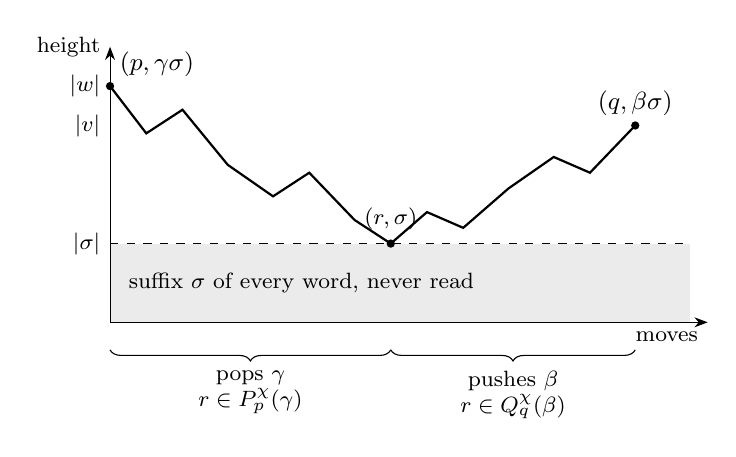
\begin{tikzpicture}[x=1.15cm,y=1.0cm,>=Stealth,font=\small]
  \fill[black!8] (0,0) rectangle (6.4,1);
  \node[font=\footnotesize,anchor=west] at (0.1,0.5)
    {suffix $\sigma$ of every word, never read};
  \draw[->] (0,0) -- (6.6,0) node[below left,font=\footnotesize] {moves};
  \draw[->] (0,0) -- (0,3.5) node[left,font=\footnotesize] {height};
  \draw[dashed] (0,1) -- (6.4,1);
  \node[left,font=\footnotesize] at (0,1) {$\len\sigma$};
  \node[left,font=\footnotesize] at (0,3) {$\len w$};
  \node[left,font=\footnotesize] at (0,2.5) {$\len v$};
  \draw[thick] (0,3) -- (0.4,2.4) -- (0.8,2.7) -- (1.3,2.0) -- (1.8,1.6)
    -- (2.2,1.9) -- (2.7,1.3) -- (3.1,1) -- (3.5,1.4) -- (3.9,1.2)
    -- (4.4,1.7) -- (4.9,2.1) -- (5.3,1.9) -- (5.8,2.5);
  \fill (0,3) circle (1.5pt) node[above right] {$(p,\gamma\sigma)$};
  \fill (3.1,1) circle (1.5pt);
  \node[above,font=\footnotesize] at (3.1,1.05) {$(r,\sigma)$};
  \fill (5.8,2.5) circle (1.5pt) node[above] {$(q,\beta\sigma)$};
  \draw[decorate,decoration={brace,amplitude=4pt,mirror}] (0,-0.35) -- (3.1,-0.35)
    node[midway,below=4pt,font=\footnotesize,align=center]
    {pops $\gamma$\\ $r\in P^\chi_{p}(\gamma)$};
  \draw[decorate,decoration={brace,amplitude=4pt,mirror}] (3.1,-0.35) -- (5.8,-0.35)
    node[midway,below=4pt,font=\footnotesize,align=center]
    {pushes $\beta$\\ $r\in Q^\chi_{q}(\beta)$};
\end{tikzpicture}
\caption{The lowest point of a pure derivation from $(p,w)$ to $(q,v)$
(\cref{lem:sm-lowest-point}). No atom on the derivation goes below the least
height $\len\sigma$, so the suffix $\sigma$ is never read: $w=\gamma\sigma$ and
$v=\beta\sigma$. The first atom $(r,\sigma)$ of least height splits the
derivation into a part summarized by the upper automaton of $p$ and a part
summarized by the lower automaton of $q$.}
\Description{A graph of word length against moves. The curve starts at the
height of w, wanders down to a lowest point at the height of sigma, and climbs
back to the height of v. A shaded band below the lowest height marks the suffix
sigma, which is never read.}
\label{fig:sm-lowest-point}
\end{figure}

\begin{lemma}[Lowest point]\label{lem:sm-lowest-point}
For signed variables $p,q$ and words $w,v$, $(p,w)\to^*_\chi(q,v)$ iff there
are cuts $i\le\len w$ and $e\le\len v$ with $\wsuf wi=\wsuf ve$ and
$P^\chi_{p,i}(w)\cap Q^\chi_{q,e}(v)\ne\varnothing$.
\end{lemma}

Cut the derivation at its first atom of least height
(\cref{fig:sm-lowest-point}) and apply \cref{lem:sm-summaries}(b,c) to the two
parts; the signed variable $r$ at the lowest point may belong to a visible or
to a hidden variable, with either sign. In the notation of
\cref{fig:sm-lowest-point}, $\gamma$ is the \emph{pop head} and $\beta$ the
\emph{push head} of the derivation.

\begin{lemma}[Duality and sign coherence]\label{lem:sm-duality}
For all signed variables $a,b,p,q$ and words $w$:
\begin{enumerate}[leftmargin=*]
\item $D_\chi(a,b)$ iff $D_\chi(\bar b,\bar a)$; hence
  $\downc\chi{\bar q}=\overline{\upc\chi q}$;
\item $Q^\chi_{\bar q}(w)=\overline{P^\chi_q(w)}$;
\item $D_\chi(a,b)$ implies $\sgn(a)=\sgn(b)$; every $r\in P^\chi_p(w)$ has
  $\sgn(r)=\sgn(p)\oplus\parity(w)$; and every $r\in Q^\chi_q(w)$ has
  $\sgn(r)=\sgn(q)\oplus\parity(w)$.
\end{enumerate}
\end{lemma}

Items (1) and (2) reverse pure derivations by duality (\cref{lem:lf-duality}):
the reversed derivation visits the same words, so it stays above the same
suffix. By item (2), \cref{lem:sm-lowest-point} can be read with upper
automata only. Item (3) is \emph{sign coherence}, the sign invariant of
\cref{lem:lf-moves}(2) applied to the derivations of \cref{lem:sm-summaries}.

\begin{example}[Shift closure: the signed system]\label{ex:sm-running}
Let $n=2$ with $f$ covariant, and let
$\psi=\{x\le z,\ z\le y,\ z\le f(z,z)\}$ be the consequent of
\cref{ex:intro-shift}, now over $\BFT$, with $z$ hidden. The copy and
constructor literals of its signed system are
\[
 x^0\le z^0,\quad z^0\le y^0,\quad z^0\le f(z^0,z^0),\quad
 y^1\le z^1,\quad z^1\le x^1,\quad f(z^1,z^1)\le z^1 .
\]
It has no facts, and its only forbidden root is $(z^0,\eps)$: the
root of $z$ is not $\Top$. Since $f$ is covariant, $(x^0,w)$ says that $\rho x$
has a leaf $\Top$ at a prefix of $w$, and $(x^1,w)$ that it has a leaf $\Bot$
at a prefix of $w$. The decomposition rule never applies, so $D_\psi$ is the
reflexive and transitive closure of the copies. Hence
$\upc\psi x^0=\{x^0,z^0,y^0\}$ and $P^\psi_{x^0}(w)=\{z^0,y^0\}$ for
$w\ne\eps$; dually, $\downc\psi x^1=\{x^1,z^1,y^1\}$ and
$Q^\psi_{x^1}(w)=\{z^1,y^1\}$ for $w\ne\eps$, as \cref{lem:sm-duality}(2)
predicts. By \cref{lem:sm-lowest-point}, $(y^1,\sigma)\to^*_\psi(x^1,\beta\sigma)$
for all words $\beta$ and $\sigma$: in every solution of $\psi$, if $y$ has a
leaf $\Bot$ at a prefix of $\sigma$, then $x$ has a leaf $\Bot$ at a prefix of
$\beta\sigma$. For trees over $\BF$ this says that every suffix of a
constructor position of $x$ is a constructor position of $y$. Similarly
$(x^0,w)\to^*_\psi(z^0,\eps)$ for every $w$, a pure derivation to the forbidden
root: $\psi$ forbids leaves $\Top$ in $x$.
\end{example}

\subsection{Least Closures of Regular Seeds}\label{sec:sm-regular}

Let
\[
 \Fup\chi=\{r:\ r\in P^\chi_e(\gamma)\text{ for some }(e,\eps)\in\Fact_\chi
 \text{ and some word }\gamma\}
\]
be the set of signed variables that a fact reaches at the empty word
after popping a word.

\begin{lemma}[The least closure]\label{lem:sm-mu}
For every signed variable $q$ and word $v$,
\[
 (q,v)\in\mu_\chi\iff Q^\chi_{q,e}(v)\cap\Fup\chi\ne\varnothing
 \text{ for some cut }e\le\len v .
\]
The set $\Fup\chi$ is the least set that contains $\upc\chi p$ for every
fact $(p,\eps)$ and contains $\pstep i(\{r\})$ for each of its
elements $r$ and each $i\in\Sigma$; it is computable in polynomial time.
\end{lemma}

A fact $(p,\eps)$ derives $(r,\sigma)$ for every $\sigma$: extend it
to $(p,\gamma\sigma)$ and pop $\gamma$. So $\mu_\chi$ contains every atom that a
pure derivation pushing a word reaches from such an $(r,\sigma)$, and
\cref{lem:lf-ext-first,lem:sm-lowest-point} show that there is nothing else.
The same argument applies to any regular set of seeds.

\begin{lemma}[Closure of regular seeds]\label{lem:sm-regular-closure}\label{prop:sm-regular-closure}
Let $S$ be a set of atoms whose slices $S_p=\{w:(p,w)\in S\}$ are regular for
all $p\in V^\pm$. For signed variables $p,r,q$, put
$U_{p,r}=\{\gamma:r\in P^\chi_p(\gamma)\}$,
$V_{r,q}=\{\beta:r\in Q^\chi_q(\beta)\}$, and
$\mathrm{Res}_{p,r}=\{\sigma:\gamma\sigma\in S_p\Sigma^*\text{ for some }
\gamma\in U_{p,r}\}$. Then the slice of $H_\chi(S)$ at $q$ is
\[
 H_\chi(S)_q=\bigcup_{r\in\Fup\chi}V_{r,q}\,\Sigma^*\ \cup\
 \bigcup_{p,r\in V^\pm}V_{r,q}\,\mathrm{Res}_{p,r}.
\]
All these languages are regular, and finite automata for them are computable
from finite automata for the slices of $S$. Consequently, whether $H_\chi(S)$
is consistent is decidable.
\end{lemma}

In particular, $\mu_\chi$ (the case $S=\varnothing$) and the closures of one
or two seeds have regular slices, and their consistency is decidable. The
lemma does not say that the set of live atoms is regular, which is
false in general (\cref{ex:sm-arrow}).

\subsection{Forbidden Roots and the Pop Bound}\label{sec:sm-cone}

A pure derivation pops a letter only at the root of an upper constructor
literal of $\chi^\pm$, and every such root is forbidden at the empty word. This
gives the \emph{pop bound}, the counterpart of the cone lemma of a covariant
system~\citep{Zhao26}, stated with the following notion and with
$\Ndown\chi=\{r:D_\chi(r,m)\text{ for some }(m,\eps)\in\Neg_\chi\}$.

\begin{definition}[Root deadness]\label{def:sm-deadu}
An atom $(p,w)$ is \emph{root-dead} in $\chi$, written $\DeadU_\chi(p,w)$, if
$\Reach_\chi(p,w)$ contains a forbidden root of $\chi$.
\end{definition}

\begin{lemma}[Roots and the pop bound]\label{lem:sm-roots}
For every signed variable $p$ and all words $w,v$:
\begin{enumerate}[leftmargin=*]
\item if $P^\chi_p(wi)\ne\varnothing$ for some letter $i$, then some
  $r\in P^\chi_p(w)$ is the root of an upper constructor literal of
  $\chi^\pm$, $(p,w)\to^*_\chi(r,\eps)$, and $(r,\eps)\in\Neg_\chi$; in
  particular $\DeadU_\chi(p,w)$;
\item \emph{(pop bound)} if $\DeadU_\chi(p,\wpre wk)$ fails, then
  $P^\chi_{p,j}(w)=\varnothing$ for every cut $j$ with $k<j\le\len w$;
\item $\DeadU_\chi(p,w)$ iff $P^\chi_p(wz)\cap\Ndown\chi\ne\varnothing$ for
  some word $z$;
\item if $\DeadU_\chi(p,wv)$, then $\DeadU_\chi(p,w)$.
\end{enumerate}
\end{lemma}

\begin{proof}
(1) If $b\in\pstep i(P^\chi_p(w))$, some $r\in P^\chi_p(w)$ is the root of an
upper constructor literal $r\le f(b_j)_j$ of $\chi^\pm$; then
$(r,\eps)\in\Neg_\chi$ by \cref{sec:lf-clauses}, and
$(p,w)\to^*_\chi(r,\eps)$ by \cref{lem:sm-summaries}(b) with $\sigma=\eps$.
(2) If $P^\chi_{p,j}(w)\ne\varnothing$ with $j>k$, then
$P^\chi_{p,k+1}(w)\ne\varnothing$, because the empty set is absorbing, and (1)
applied to $\wpre wk$ and the letter $w[k]$ gives $\DeadU_\chi(p,\wpre wk)$.
(3) By \cref{lem:lf-ext-first}, $(m,\eps)\in \Reach_\chi(p,w)$ iff
$(p,w\alpha)\to^*_\chi(m,\eps)$ for some $\alpha$; by
\cref{lem:sm-lowest-point} with the empty word $v=\eps$, whose only cut is $0$,
this holds iff $P^\chi_p(w\alpha)\cap\downc\chi m\ne\varnothing$. (4) By
\cref{lem:lf-closure}(4), $(p,wv)\in \Reach_\chi(p,w)$, so
$\Reach_\chi(p,wv)\subseteq \Reach_\chi(p,w)$.
\end{proof}

\subsection{Deadness}\label{sec:sm-dead}

\Cref{cor:lf-dead} lists three causes of deadness for a satisfiable system:
(a) a forbidden root in $\Reach_\chi(p,w)$, which is $\DeadU_\chi(p,w)$; (b) the
opposite of an extension of the seed in $\mu_\chi$; and (c) a self-collision,
the opposite of an extension of the seed in $\Reach_\chi(p,w)$. The causes may
overlap. Causes (a) and (b) together are deadness by support, which automata
read. A self-collision of an atom that is not dead by support is read by a
strict comparison of the seed word.

\begin{definition}[Deadness by support, self events]\label{def:sm-dead}
An atom $(p,w)$ is \emph{dead by support} in $\chi$, written
$\DeadT_\chi(p,w)$, if $\DeadU_\chi(p,w)$ or $(\bar p,w\delta)\in\mu_\chi$ for
some word $\delta$. A \emph{self event} of $(p,w)$ in $\chi$ is a comparison
$(i,j)$ of $w$ (\cref{def:bg-comparison}), that is, a pair of cuts
$0\le i<j\le\len w$ with $\wsuf wj\pre\wsuf wi$, such that
\[
 P^\chi_{p,i}(w)\cap\overline{P^\chi_{p,j}(w)}\ne\varnothing .
\]
Self events are strict: $i<j$. We write $\SelfEv_\chi(p,w,i,j)$ if $(i,j)$ is
a self event of $(p,w)$.
\end{definition}

Self events have a counterpart in the plain-entailment proof, whose readers
already compare a root with its own signed copy \citep{Zhao26}. Here
both cuts belong to the word of one seed: the state of the upper automaton of
$p$ at the cut $i$ and the flipped state at the cut $j$ share a signed
variable, which serves as the lowest point of a pure derivation from an
extension of $(p,w)$ to the opposite of an extension of $(p,w)$
(\cref{thm:sm-dead}).

Both kinds of deadness by support are read by the upper automaton of $p$
together with one bit. Put
\[
 \DeadU^\eps_\chi=\{r\in V^\pm:\DeadU_\chi(r,\eps)\},\qquad
 \DeadT^\eps_\chi=\{r\in V^\pm:\DeadT_\chi(r,\eps)\}.
\]

\begin{lemma}[Deadness from states]\label{lem:sm-dead-states}
For every signed variable $p$ and all words $w$, $v$:
\begin{enumerate}[leftmargin=*]
\item $\DeadU_\chi(p,w)$ iff $P^\chi_p(w)\cap\DeadU^\eps_\chi\ne\varnothing$;
\item $(\bar p,w)\in\mu_\chi$ iff
  $\overline{P^\chi_{p,e}(w)}\cap\Fup\chi\ne\varnothing$ for some cut
  $e\le\len w$;
\item $\DeadT_\chi(p,w)$ iff $(\bar p,w)\in\mu_\chi$ or
  $P^\chi_p(w)\cap\DeadT^\eps_\chi\ne\varnothing$;
\item if $\DeadT_\chi(p,wv)$, then $\DeadT_\chi(p,w)$;
\item the sets $\DeadU^\eps_\chi$ and $\DeadT^\eps_\chi$ are computable in
  polynomial time.
\end{enumerate}
\end{lemma}

So the words $w$ with $\DeadU_\chi(p,w)$, and those with $\DeadT_\chi(p,w)$,
form regular languages that are closed under prefixes: the first is read by
the upper automaton of $p$, and the second by that automaton together with a
bit that records whether some state $P$ read so far has
$\bar P\cap\Fup\chi\ne\varnothing$. Self events, in contrast, compare two cuts
of one word. They are what remains of deadness.

\begin{theorem}[Deadness]\label{thm:sm-dead}
Let $\chi$ be satisfiable. An atom $(p,w)$ is dead iff $\DeadT_\chi(p,w)$ or
$(p,w)$ has a self event in $\chi$. More precisely, every self event of $(p,w)$
yields a self-collision of $(p,w)$, and if $(p,w)$ has a self-collision but
$\DeadT_\chi(p,w)$ fails, then $(p,w)$ has a self event.
\end{theorem}

By \cref{cor:lf-dead}, it remains to treat a self-collision, a pure
derivation from an extension $(p,w\alpha)$ to an opposite atom
$(\bar p,w\delta)$, of an atom $(p,w)$ that is not dead by support. Split it
at its lowest point. If its pop head or its push head is longer than $w$, then the upper automaton of $p$ is
nonempty after some proper extension of $w$ (for the push head, by
\cref{lem:sm-duality}(2)), and the pop bound (\cref{lem:sm-roots}) gives
$\DeadU_\chi(p,w)$. Otherwise both heads end at cuts $i,j$ of $w$, the
suffixes $\wsuf wi$ and $\wsuf wj$ are comparable in the prefix order, and by
\cref{lem:sm-duality}(2) the lowest point lies in
$P^\chi_{p,i}(w)\cap\overline{P^\chi_{p,j}(w)}$. Sign coherence excludes
$i=j$, and the condition is symmetric in $i$ and $j$, so the shorter suffix is
a prefix of the longer one and $(i,j)$ or $(j,i)$ is a strict self event.
Conversely, every self event yields a self-collision. The proof is in
\cref{app:sm}.

\begin{example}[A nonregular dead language]\label{ex:sm-arrow}
Let $\varphi=\{x\le x\to x\}$ for the arrow, as in
\cref{ex:lf-clauses,ex:lf-least}. The copy and constructor literals of
$\varphi^\pm$ are $x^0\le f(x^1,x^0)$ and $f(x^0,x^1)\le x^1$, there are no
facts, so $\mu_\varphi=\varnothing$, and the only forbidden root is
$(x^0,\eps)$. The closure $D_\varphi$ is the identity, and
\[
 P^\varphi_{x^0}(1^k)=\{x^0\},\qquad P^\varphi_{x^0}(1^k0)=\{x^1\},\qquad
 P^\varphi_{x^0}(w)=\varnothing\ \text{if $1^k0$ is a proper prefix of $w$}.
\]
Hence $\DeadT^\eps_\varphi=\{x^0\}$, and $\DeadT_\varphi(x^0,w)$ holds iff
$w\in1^*$. The guard of a self event $(i,j)$ requires
$P^\varphi_{x^0,i}(w)=\{x^0\}$ and $P^\varphi_{x^0,j}(w)=\{x^1\}$, so
$w=1^k0v$, $i\le k$, and $j=k+1$; the comparison requires $v\pre1^m0v$ with
$m=k-i$, that is, $v\pre(1^m0)^\omega$ (\cref{lem:bg-periodic}). By
\cref{thm:sm-dead}, the dead words of $x^0$ are
\[
 1^*\ \cup\ \{1^k0v:\ v\pre(1^m0)^\omega\text{ for some }m\le k\}.
\]
This language is not regular: its intersection with $1^*01^*0$ is
$\{1^k01^m0:m\le k\}$. For example, $(x^0,0)$ is dead by the self event
$(0,1)$ of the word $0$, although $\DeadT_\varphi(x^0,0)$ fails. This is the
self event that the proof of \cref{thm:sm-dead} extracts from the
self-collision $(x^0,00)\to(x^1,0)$ of \cref{ex:lf-least}: its lowest point
$(x^1,0)$ lies at the cut $1$ of $00$ and the cut $0$ of $0$. The atom
$(x^0,01)$ is live (\cref{ex:lf-least}).
\end{example}

\begin{remark}[No self events without mixed parity]\label{rem:sm-parity}
If $\chi$ has a parity assignment $\pi$ (\cref{rem:ch-parity}), then every
pure move preserves $\sgn(r)\oplus\pi(r)$, where $\pi(x^\pm)=\pi(x)$, so every
$r\in P^\chi_p(w)$ has $\sgn(r)\oplus\pi(r)=\sgn(p)\oplus\pi(p)$. Hence no set
$P^\chi_{p,i}(w)$ meets a flipped set $\overline{P^\chi_{p,j}(w)}$, $\chi$ has no
self events, deadness in a satisfiable $\chi$ is $\DeadT_\chi$, and the live
words of each signed variable form a regular language. This is the automaton
form of \cref{rem:ch-parity}; it includes covariant systems, with $\pi=0$.
\end{remark}

\subsection{Closure Membership}\label{sec:sm-membership}

\begin{lemma}[Closure membership]\label{lem:sm-membership}
Let $(p,w)$ be live in $\chi$, and let $(q,v)$ be an atom. Then
$(q,v)\in\Cl_\chi(p,w)$ iff $(q,v)\in\mu_\chi$ or there are cuts $i\le\len w$
and $e\le\len v$ with
\[
 \wsuf wi\pre\wsuf ve\qquad\text{and}\qquad
 P^\chi_{p,i}(w)\cap Q^\chi_{q,e}(v)\ne\varnothing .
\]
\end{lemma}

\begin{proof}
By \cref{lem:lf-ext-first,lem:sm-lowest-point}, $(q,v)\in \Reach_\chi(p,w)$ iff
there are a word $\alpha$ and cuts $i\le\len{w\alpha}$, $e\le\len v$ with
$\wsuf{(w\alpha)}i=\wsuf ve$ and
$P^\chi_p(\wpre{(w\alpha)}i)\cap Q^\chi_{q,e}(v)\ne\varnothing$. If
$i>\len w$, then $P^\chi_p(w\alpha')\ne\varnothing$ for the nonempty prefix
$\alpha'$ of $\alpha$ of length $i-\len w$, and \cref{lem:sm-roots}(2) with
$k=\len w$ gives $\DeadU_\chi(p,w)$, so $\Cl_\chi(p,w)$ contains a forbidden
root, contradicting liveness by \cref{lem:lf-closure}(2). Hence $i\le\len w$,
and the equation reads $\wsuf wi\,\alpha=\wsuf ve$, which gives
$\wsuf wi\pre\wsuf ve$. Conversely, if $\wsuf wi\,\alpha=\wsuf ve$ and the
intersection is nonempty, \cref{lem:sm-lowest-point} gives
$(p,w\alpha)\to^*_\chi(q,v)$, and $(p,w\alpha)\in \Reach_\chi(p,w)$.
\end{proof}

The two cuts belong to different words, so there is no restriction $i<e$.
The prefix relation points from the seed to the consequence: the seed word may
be continued to the word of the consequence, because extensions are rules.

\subsection{Heads of Derivations}\label{sec:sm-heads}

The pop head of a pure derivation passes only through root-dead atoms.
Immediately before a pop, the signed variable of the current atom is the root
of an upper constructor literal, whose empty-word atom is forbidden.

\begin{lemma}[Head prefixes]\label{lem:sm-head-prefix}
If $P^\chi_p(\gamma)\ne\varnothing$, then $\DeadU_\chi(p,\wpre\gamma i)$ for
every $i<\len\gamma$.
\end{lemma}

\begin{proof}
Since the empty set is absorbing, $P^\chi_p(\wpre\gamma{i+1})\ne\varnothing$,
and \cref{lem:sm-roots}(1) applies to $\wpre\gamma i$ and the letter
$\gamma[i]$.
\end{proof}

The lemma uses neither satisfiability nor any condition relating two systems.
Applied to $\psi$, it says that every proper prefix $\gamma'$ of the pop head
$\gamma$ of a pure derivation of $\psi$ from a visible atom $(p,\gamma\sigma)$
has $\DeadU_\psi(p,\gamma')$; under condition \CondU, the atom $(p,\gamma')$ is
then dead in $\varphi$ (\cref{def:ch-conditions,def:sm-deadu}). \Cref{sec:ex}
uses this to end every pop head of $\psi$ at or before the first rejected cut
of the seed (\cref{lem:ex-fh,lem:ex-head-before-J}).

\subsection{Satisfiability and Condition (I0)}\label{sec:sm-decide}

\begin{proposition}[Satisfiability and (I0)]\label{prop:sm-decide}
\leavevmode
\begin{enumerate}[leftmargin=*]
\item A system $\chi$ is satisfiable iff $\downc\chi m\cap\Fup\chi=\varnothing$
  for every forbidden root $(m,\eps)$ and there are no variable $x$ and word
  $w$ with $(x^+,w),(x^-,w)\in\mu_\chi$.
\item Let $\varphi$ be a system over $X$ and $\psi$ a system over $X\cup Z$.
  Condition \CondI, $\mu_\psi|_X\subseteq\mu_\varphi$, fails iff some
  $q\in X^\pm$ and some word $v$ have $(q,v)\in\mu_\psi$ and
  $(q,v)\notin\mu_\varphi$.
\end{enumerate}
Satisfiability and condition \CondI\ are decidable in polynomial space.
\end{proposition}

\begin{proof}
(1) By \cref{lem:lf-closure}(2), $\chi$ is satisfiable iff $\mu_\chi$ is
consistent, that is, contains no forbidden root and no exclusion pair. By
\cref{lem:sm-mu} with $v=\eps$, $(m,\eps)\in\mu_\chi$ iff
$\downc\chi m\cap\Fup\chi\ne\varnothing$. (2) is the definition of \CondI. For
the complexity, \cref{lem:sm-mu} reads membership in $\mu_\chi$ at $q$ by the
lower automaton of $q$ together with a bit that records whether some state
read so far met $\Fup\chi$. The second condition of (1) is therefore
reachability, for some $x\in V$, of a state with both bits set in the product
of the lower automata of $x^+$ and $x^-$, each with its bit; and the condition
of (2) is reachability, for some $q\in X^\pm$, of a state whose $\psi$-bit is
set and whose $\varphi$-bit is not, in the product of the lower automata of
$q$ in $\psi$ and in $\varphi$. A state of these products has a description of
polynomial size, its successors are computable in polynomial time, and
reachability is decided by guessing a path state by state, in nondeterministic
polynomial space, hence in polynomial space. The set $\Fup\chi$ is computable
in polynomial time by \cref{lem:sm-mu}.
\end{proof}

A shortest witness of the second condition of (1), or of a failure of \CondI,
is shorter than the number of states of the product automaton. Condition
\CondU\ needs more than reachability, because liveness involves self events; it
is the subject of \cref{sec:un}.

%% units.tex -- condition (U) as a plain single-word hole problem: the source
%% automaton, the unit reader with the rejected-path property, and the decision
%% of (U) by the hole search of Zhao26 on the unit reader. The smaller reader
%% and the antecedent rejection clock, used only for the complexity bounds, are
%% in the unmechanized part (complexity.tex, sec:un-smaller). Proofs:
%% appendix-summaries.tex (app:sm).

\section{Condition (U)}\label{sec:un}

From now on, $\varphi$ is a system over the visible variables $X$ and $\psi$ a
system over $X\cup Z$, as in \cref{sec:ch}. Condition \CondU\ of
\cref{def:ch-conditions} asks that $\Reach_\psi(a)$ contain no forbidden root of
$\psi$ for every visible atom $a$ that is live in $\varphi$. In the terms of
\cref{def:sm-deadu}, this reads as follows.

\begin{lemma}[Condition (U)]\label{lem:un-dead}
Condition \CondU\ holds iff no $p\in X^\pm$ and no word $w$ satisfy
$\DeadU_\psi(p,w)$ while $(p,w)$ is live in $\varphi$.
\end{lemma}

The words $w$ with $\DeadU_\psi(p,w)$ form a regular language
(\cref{lem:sm-dead-states}), but the words $w$ with $(p,w)$ live in $\varphi$
need not (\cref{ex:sm-arrow}), so \CondU\ is not an inclusion of regular
languages. When $\varphi$ is satisfiable, however, \cref{thm:sm-dead}
identifies liveness with the absence of $\DeadT_\varphi$, which is regular,
and of self events, which are comparisons of a single word whose two cuts are
tested by a pair of automaton states. A failure of \CondU\ is therefore a hole of a reader in the sense of
\citet{Zhao26} (\cref{def:bg-reader,def:bg-hole}), and the reader has the
rejected-path property (\cref{def:bg-rpp}). The hole search of that paper
(\cref{cor:bg-hole-decision}) then decides \CondU.

\subsection{The Source Automaton}\label{sec:un-automaton}

One automaton reads the word of a visible seed for both systems. The two-word
instances of \cref{sec:ex} use it again, on the seed word.

\begin{definition}[Source automaton]\label{def:un-source}
Let $p\in X^\pm$. The \emph{source automaton} $\Bsrc_p$ is the deterministic
automaton over $\Sigma$ whose states are the triples $\zeta=(P,b,P')$ with
$P\subseteq X^\pm$, $b\in\{0,1\}$, and $P'\subseteq(X\cup Z)^\pm$, with start
state $\bigl(\upc\varphi p,\ [\overline{\upc\varphi p}\cap\Fup\varphi\ne
\varnothing],\ \upc\psi p\bigr)$ and transitions
\[
 \delta\bigl((P,b,P'),i\bigr)=\bigl(\pstep i(P),\
 b\lor[\overline{\pstep i(P)}\cap\Fup\varphi\ne\varnothing],\
 \pstep i(P')\bigr),
\]
where the first component uses the transitions of the upper automata of
$\varphi$ and the third those of $\psi$, and $[\,\cdot\,]$ is $1$ for a true
condition and $0$ otherwise. For a state $\zeta=(P,b,P')$ put
\[
 \mathrm{dt}(\zeta)\iff b=1\ \text{or}\ P\cap\DeadT^\eps_\varphi\ne\varnothing,
 \qquad
 \mathrm{du}(\zeta)\iff P'\cap\DeadU^\eps_\psi\ne\varnothing,
\]
and let the \emph{self guard} $\GuardS$ consist of the pairs of states
$((P_1,b_1,P'_1),(P_2,b_2,P'_2))$ with $P_1\cap\overline{P_2}\ne\varnothing$.
\end{definition}

\begin{lemma}[Runs of the source automaton]\label{lem:un-source}
Let $p\in X^\pm$, let $w$ be a word, and let $\zeta_j$ be the state of
$\Bsrc_p$ after $\wpre wj$. Then:
\begin{enumerate}[leftmargin=*]
\item $\zeta_j=\bigl(P^\varphi_{p,j}(w),\ [(\bar p,\wpre wj)\in\mu_\varphi],\
  P^\psi_{p,j}(w)\bigr)$;
\item $\mathrm{dt}(\zeta_j)$ iff $\DeadT_\varphi(p,\wpre wj)$, and
  $\mathrm{du}(\zeta_j)$ iff $\DeadU_\psi(p,\wpre wj)$; if
  $\mathrm{dt}(\zeta_j)$ fails, it fails at every later cut, and if
  $\mathrm{du}(\zeta_j)$ holds, it holds at every earlier cut;
\item for $i<j\le\len w$, the pair $(i,j)$ is a self event of $(p,w)$ in
  $\varphi$ iff it is a comparison of $w$ and $(\zeta_i,\zeta_j)\in\GuardS$.
\end{enumerate}
The automaton $\Bsrc_p$ has $N_{\mathrm U}=2^{4\len X+2\len Z+1}$ states.
\end{lemma}

Item (1) holds by induction on $j$, using \cref{lem:sm-dead-states}(2) for
the bit; item (2) is \cref{lem:sm-dead-states}(1,3) together with
\cref{lem:sm-roots}(4) and \cref{lem:sm-dead-states}(4); and item (3) is
\cref{def:sm-dead}. The sets $\Fup\varphi$, $\DeadT^\eps_\varphi$, and
$\DeadU^\eps_\psi$ are computable (\cref{lem:sm-mu,lem:sm-dead-states}), so
$\Bsrc_p$, $\mathrm{dt}$, $\mathrm{du}$, and $\GuardS$ are computable.

\subsection{The Unit Reader}\label{sec:un-reader}

\begin{definition}[Unit reader]\label{def:un-reader}
For $p\in X^\pm$, the \emph{unit reader} is the reader
$\RU(p)=(\Bsrc_p,\GuardS,\Rej_{\mathrm U})$ with the source automaton, the
self guard as its admission relation, and the rejected states
\[
 \Rej_{\mathrm U}=\{\zeta:\ \mathrm{dt}(\zeta)\text{ fails and }
 \mathrm{du}(\zeta)\text{ holds}\}.
\]
\end{definition}

\begin{lemma}[Holes of the unit reader]\label{lem:un-holes}
Let $\varphi$ be satisfiable and $p\in X^\pm$. A word $w$ is a hole of
$\RU(p)$ iff $(p,w)$ is live in $\varphi$ and $\DeadU_\psi(p,w)$.
Consequently, \CondU\ holds iff none of the $2\len X$ unit readers has a hole.
\end{lemma}

\begin{proof}
By \cref{lem:un-source}, $w$ is rejected iff $\DeadT_\varphi(p,w)$ fails and
$\DeadU_\psi(p,w)$ holds, and a comparison of $w$ is admitted iff it is a self
event of $(p,w)$ in $\varphi$. So $w$ is a hole iff $\DeadU_\psi(p,w)$ holds
and $(p,w)$ is neither dead by support nor has a self event in $\varphi$, that
is, by \cref{thm:sm-dead}, iff $\DeadU_\psi(p,w)$ holds and $(p,w)$ is live in
$\varphi$. The second claim follows by \cref{lem:un-dead}.
\end{proof}

\begin{lemma}[Rejected paths]\label{lem:un-rejected-path}
Every unit reader $\RU(p)$ has the rejected-path property: it satisfies
betweenness and the admission cone. No satisfiability assumption is needed.
\end{lemma}

\begin{proof}
\emph{Betweenness.} Let $\wpre wa$ and $\wpre wb$ be rejected, with $a<k<b$.
Since $\mathrm{dt}$ fails at $a$, it fails at $k$, and since $\mathrm{du}$
holds at $b$, it holds at $k$ (\cref{lem:un-source}(2)). So $\wpre wk$ is
rejected.

\emph{Admission cone.} Let $w$ be rejected, with first rejected cut $J$, and
let $(i,j)$ be an admitted comparison of $w$. The guard
$P^\varphi_{p,i}(w)\cap\overline{P^\varphi_{p,j}(w)}\ne\varnothing$ requires
$P^\varphi_{p,j}(w)\ne\varnothing$. At the cut $J$, $\mathrm{dt}$ fails, so
$\DeadT_\varphi(p,\wpre wJ)$ fails, and in particular
$\DeadU_\varphi(p,\wpre wJ)$ fails. The pop bound (\cref{lem:sm-roots}(2)) gives
$P^\varphi_{p,j'}(w)=\varnothing$ for every $j'>J$. Hence $j\le J$.
\end{proof}

The proof gives more than the admission cone: no admission, comparison or not, has its
second cut after $J$.

\begin{example}[Shift closure: condition (U)]\label{ex:un-running}
Let $\psi=\{x\le z,\ z\le y,\ z\le f(z,z)\}$ as in \cref{ex:sm-running}, with
$f$ binary and covariant, and let $\varphi_1=\{x\le y\}$. Over $\BFT$,
condition \CondU\ fails. Indeed, $\DeadU^\eps_\psi=\{x^0,z^0\}$ and
$z^0\in P^\psi_{x^0}(w)$ for every $w$, so $\DeadU_\psi(x^0,w)$ holds for every
word $w$. On the other side, $\varphi_1$ has neither facts nor
forbidden roots, so $\DeadT_{\varphi_1}$ never holds, and it has no upper
constructor literal, so $P^{\varphi_1}_{x^0}(w)=\varnothing$ for $w\ne\eps$ and
no comparison is admitted. Every word is a hole of $\RU(x^0)$, the empty word
included. Its countermodel is the least model $\Cl_{\varphi_1}(x^0,\eps)$, the
solution $x=y=\Top$: no $z$ satisfies $\Top\le z\le f(z,z)$.

Over $\BF$, the variables cannot take the value $\Top$. Within $\BFT$, this
can be expressed by a variable $g$ with $y\le g$ and $g\le f(g,g)$, which
allow exactly the trees $y$ without leaves $\Top$; this is the gadget of
\cref{lem:tc-gadget}. The reduction of \cref{thm:tc-gadget} puts such a gadget
on every variable, but for this example one on $y$ suffices: since $x\le y$, it also
keeps $x$ free of $\Top$, and $z\le f(z,z)$ already keeps $z$ free of $\Top$.
So let $\varphi'_1=\{x\le y,\ y\le g,\ g\le f(g,g)\}$, with $g$ visible. Its only
forbidden root is $(g^0,\eps)$, and $x^0\to y^0\to g^0$ by copies, after which
$g^0$ pops every word. So $\DeadT_{\varphi'_1}(x^0,w)$ holds for every $w$, and
$\RU(x^0)$ rejects no word. For the other signed variables
$p\in\{x^1,y^0,y^1,g^0,g^1\}$, the set $P^\psi_p(w)$ never meets
$\DeadU^\eps_\psi$, so $\RU(p)$ rejects no word either. Thus \CondU\ holds for
$\varphi'_1$; \cref{ex:ex-running} shows that the entailment fails by
condition \CondII.
\end{example}

\begin{example}[Admitted self events are needed]\label{ex:un-arrow}
Let $\varphi=\{x\le x\to x\}$ as in \cref{ex:sm-arrow}, and let
$\psi=\{x\le a\to x,\ c\to y\le a\}$ with $a,c$ hidden. The antecedent is that
of \cref{ex:ch-arrow}, but the consequent is new. For $x\le z\to z$,
\CondU\ holds because its only root-dead atom, $(x^0,\eps)$, is a forbidden
root of $\varphi$ as well; this consequent is chosen so that \CondU\ holds only
because of admitted self events. The signed system of
$\psi$ has the upper constructor literals $x^0\le f(a^1,x^0)$ and
$a^1\le f(c^0,y^1)$ and the lower ones $f(a^0,x^1)\le x^1$ and
$f(c^1,y^0)\le a^0$; its closure is the identity, and
$\DeadU^\eps_\psi=\{x^0,a^1\}$. Reading from $x^0$,
\[
 P^\psi_{x^0}(1^k)=\{x^0\},\quad P^\psi_{x^0}(1^k0)=\{a^1\},\quad
 P^\psi_{x^0}(1^k00)=\{c^0\},\quad P^\psi_{x^0}(1^k01)=\{y^1\},
\]
and the empty set after longer words. So $\DeadU_\psi(x^0,w)$ holds iff
$w\in1^*\cup1^*0$, and $\RU(x^0)$ rejects exactly the words $1^k0$, which are
not dead by support in $\varphi$. Each of them has the admitted comparison
$(0,k+1)$: $P^\varphi_{x^0}(\eps)=\{x^0\}$ meets
$\overline{P^\varphi_{x^0}(1^k0)}=\{x^0\}$. So $\RU(x^0)$ has no hole. The other
unit readers reject no word, because $x^1$, $y^0$, and $y^1$ have no root-dead
atoms in $\psi$. Hence \CondU\ holds. Without the admitted self events, the
word $0$ would be a hole: $(x^0,0)$ is dead in $\varphi$ only through its self event
(\cref{ex:sm-arrow}).
\end{example}

\Cref{fig:un-reader} draws this reader. The admission relation acts as a
rescue: a rejected word, a candidate failure of \CondU, is discarded as soon
as two of its cuts form a comparison with an admitted pair of states, because
the seed is then dead in $\varphi$. A small change of the consequent, also
shown there, leaves a rejected word that no comparison rescues, a hole.

\begin{figure}[tbp]
\centering
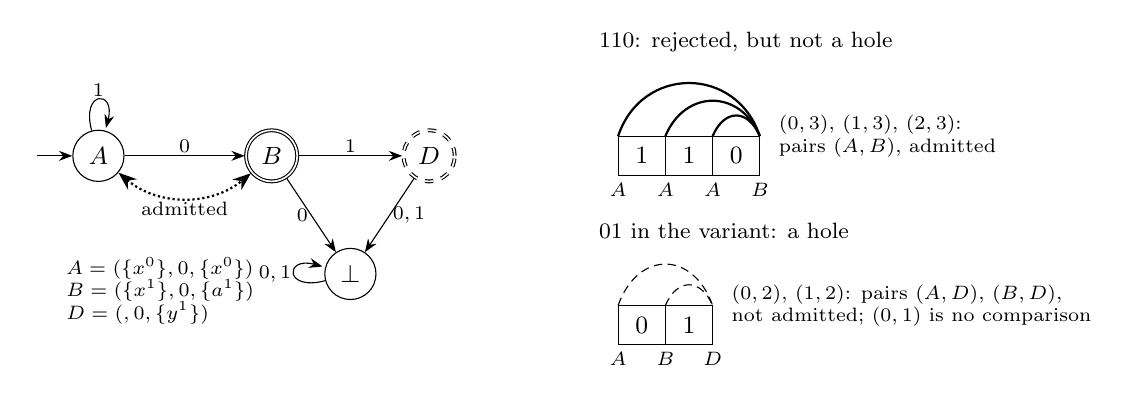
\begin{tikzpicture}[>=Stealth,font=\small,x=1cm,y=1cm,
    every node/.style={inner sep=1.5pt},
    st/.style={state,minimum size=6.5mm,inner sep=0pt},
    lb/.style={font=\scriptsize,inner sep=1pt},
    cell/.style={draw,minimum width=6mm,minimum height=5mm,inner sep=0pt},
    adm/.style={thick},
    nadm/.style={densely dashed}]
  % the reduced unit reader R_U(x^0)
  \node[st,initial,initial text={}] (A) at (0,0) {$A$};
  \node[st,accepting] (B) at (2.2,0) {$B$};
  \node[st,accepting,dashed] (D) at (4.2,0) {$D$};
  \node[st] (S) at (3.2,-1.5) {$\bot$};
  \path[->] (A) edge[loop above] node[lb,above]{$1$} (A)
            (A) edge node[lb,above]{$0$} (B)
            (B) edge node[lb,above]{$1$} (D)
            (B) edge node[lb,left]{$0$} (S)
            (D) edge node[lb,right]{$0,1$} (S)
            (S) edge[loop left] node[lb,left]{$0,1$} (S);
  \draw[<->,adm,densely dotted] (A) to[bend right=40] node[lb,below]{admitted} (B);
  \node[lb,anchor=north west,align=left] at (-0.45,-1.25)
    {$A=(\{x^0\},0,\{x^0\})$\\ $B=(\{x^1\},0,\{a^1\})$\\ $D=(\varnothing,0,\{y^1\})$};
  % the word 110
  \begin{scope}[xshift=6.6cm]
    \node[font=\footnotesize,anchor=west] at (-0.3,1.45) {$110$: rejected, but not a hole};
    \foreach \l [count=\i from 0] in {1,1,0}
      \node[cell] at (0.6*\i+0.3,0) {$\l$};
    \foreach \q [count=\i from 0] in {A,A,A,B}
      \node[lb,anchor=north] at (0.6*\i,-0.3) {$\q$};
    \draw[adm] (0,0.25) .. controls (0.3,1.15) and (1.5,1.15) .. (1.8,0.25);
    \draw[adm] (0.6,0.25) .. controls (0.85,0.85) and (1.55,0.85) .. (1.8,0.25);
    \draw[adm] (1.2,0.25) .. controls (1.35,0.6) and (1.65,0.6) .. (1.8,0.25);
    \node[lb,anchor=west,align=left] at (2.0,0.25) {$(0,3)$, $(1,3)$, $(2,3)$:\\ pairs $(A,B)$, admitted};
  \end{scope}
  % the word 01, variant
  \begin{scope}[xshift=6.6cm,yshift=-2.15cm]
    \node[font=\footnotesize,anchor=west] at (-0.3,1.2) {$01$ in the variant: a hole};
    \foreach \l [count=\i from 0] in {0,1}
      \node[cell] at (0.6*\i+0.3,0) {$\l$};
    \foreach \q [count=\i from 0] in {A,B,D}
      \node[lb,anchor=north] at (0.6*\i,-0.3) {$\q$};
    \draw[nadm] (0,0.25) .. controls (0.25,0.95) and (0.95,0.95) .. (1.2,0.25);
    \draw[nadm] (0.6,0.25) .. controls (0.75,0.6) and (1.05,0.6) .. (1.2,0.25);
    \node[lb,anchor=west,align=left] at (1.4,0.25) {$(0,2)$, $(1,2)$: pairs $(A,D)$, $(B,D)$,\\ not admitted; $(0,1)$ is no comparison};
  \end{scope}
\end{tikzpicture}
\caption{The unit reader $\RU(x^0)$ of \cref{ex:un-arrow}, after merging the
states that cannot occur on a rejected word into a sink $\bot$
(\cref{lem:un-reduced}). Rejected states are doubly circled; the only admitted
pairs are $(A,B)$ and $(B,A)$, the self guard of the antecedent $x\le x\to x$.
Every rejected word $1^k0$, such as $110$, ends in $B$ and has the terminal
comparisons $(i,k+1)$ with the admitted pair $(A,B)$: it is rescued, because
$(x^0,1^k0)$ is dead in $\varphi$ by a self event. In the example itself the
state $D$, dashed, is not rejected and would be merged into $\bot$. In a
variant in which $y$ is hidden and $\psi$ also contains $d\to e\le y$, with
$d,e$ hidden, the atom $(y^1,\eps)$ is a forbidden root, $D$ is rejected, and
the word $01$ is a hole: none of its comparisons is admitted, so $(x^0,01)$ is
live in $\varphi$ and root-dead in $\psi$, and \CondU\ fails.}
\Description{Left: an automaton with states A, B, D and a sink bottom. A is the
start state with a loop on 1; 0 leads from A to B, 1 from B to D, 0 from B to
the sink, and both letters from D to the sink, which loops on both letters. B
is doubly circled, D doubly circled and dashed. A dotted double arrow labeled
admitted joins A and B. A legend lists the triples of the states A, B and D. Right: the
word 110 with the states A, A, A, B at its cuts and three solid arcs from the
cuts 0, 1 and 2 to the cut 3, labeled admitted; below, the word 01 with the states
A, B, D and two dashed arcs from the cuts 0 and 1 to the cut 2, labeled not
admitted.}
\label{fig:un-reader}
\end{figure}


\subsection{Deciding Condition (U)}\label{sec:un-decide}

\Citet{Zhao26} decides the hole problem for every reader with the
rejected-path property (\cref{cor:bg-hole-decision}): a reader with $N$ states
over a finite alphabet that has this property has a hole iff it has a hole of
length at most $\holeBound(N,d_N)$, where $d_N=2N(4N-1)-1$. The proof selects a
hole with rejected tail at most $4N-2$ (\cref{thm:bg-brt}), bounds its depth
(\cref{thm:bg-depth}), and shortens it (\cref{thm:bg-search}). Applied to the
unit readers, with their $N_{\mathrm U}$ states, this decides \CondU.

\begin{theorem}[Condition (U) is decidable]\label{thm:un-decidable}
Let $\varphi$ be satisfiable, and let $N_{\mathrm U}=2^{4\len X+2\len Z+1}$ be
the number of states of the source automaton. Condition \CondU\ fails iff
there are $p\in X^\pm$ and a word $w$ with
$\len w\le\holeBound(N_{\mathrm U},d_{N_{\mathrm U}})$ such that $(p,w)$ is
live in $\varphi$ and $\DeadU_\psi(p,w)$. Hence \CondU\ is decidable. If
$X\ne\varnothing$, then, with $v=\len X$, $s=\len X+\len Z$ and
$E_3(x)=2^{2^{2^x}}$,
\[
 \holeBound(N_{\mathrm U},d_{N_{\mathrm U}})\le E_3(10v+10s+17)\le E_3(20s+17).
\]
The bound depends neither on the arity nor on the variance.
\end{theorem}

\begin{proof}
By \cref{lem:un-holes}, \CondU\ fails iff some unit reader $\RU(p)$ has a
hole. Each $\RU(p)$ has $N_{\mathrm U}$ states, the finite alphabet $\Sigma$,
and the rejected-path property (\cref{lem:un-rejected-path}), so by
\cref{cor:bg-hole-decision} it has a hole iff it has one of length at most
$\holeBound(N_{\mathrm U},d_{N_{\mathrm U}})$, and by \cref{lem:un-holes} such
a hole is a word as stated. If $X$ is empty, there is no unit reader and
\CondU\ holds. For the decision, enumerate the $2\len X$ signed variables and
the finitely many words up to this length, and test each pair by
\cref{lem:un-source}: the states of $\Bsrc_p$ along $w$ are computable, and so
are rejection and the admission of each of the finitely many comparisons of
$w$.

For the estimate, let $v\ge1$. Then $N_{\mathrm U}=2^{2v+2s+1}\ge8$, so
$N_{\mathrm U}+1\le\frac98N_{\mathrm U}$, and $(\frac98)^5<2$. By
\cref{cor:bg-hole-decision}, $\holeBound(N_{\mathrm U},d_{N_{\mathrm U}})\le
2^{2^{1280(N_{\mathrm U}+1)^5}}$, and
$1280(N_{\mathrm U}+1)^5<2^{12}N_{\mathrm U}^5=2^{10v+10s+17}$; finally
$v\le s$.
\end{proof}

The bound of \cref{thm:un-decidable} is not the smallest one. A smaller reader
gives a sharper bound (\cref{prop:un-sharper}); it serves only the complexity
analysis and is therefore placed in the part that is not mechanized
(\cref{sec:un-smaller}).

Informally, a different route would reduce \CondU\ to plain entailment: the
words $w$ with $\DeadU_\psi(p,w)$ form a regular language $W_p$, and \CondU\
asks that in every solution of $\varphi$ the leaf cone of $p$ avoid $W_p$, a
comparison with a regular ground tree determined by $W_p$. We do not pursue
this route; the unit reader gives an explicit witness bound without additional
variables. \Cref{sec:ex} turns to condition \CondII.

%% extraction.tex -- the two-word hole problem with target self events, forced
%% target heads (FH), the extracted instances I_pq with enriched rejection
%% (neither dead by support nor root-dead), FH by construction, and the theorem
%% that under satisfiability and (U), condition (II) holds iff no extracted
%% instance has a hole. Proofs: appendix-summaries.tex (app:sm).

\section{Two-Word Holes with Self Events}\label{sec:ex}

Condition \CondII\ fails when a visible atom that is live in $\varphi$ has a
visible $\psi$-consequence outside its closure in $\varphi$; by
\cref{lem:ch-pure}(2), the consequence can be taken to be derived by a pure
derivation. By the lowest point (\cref{lem:sm-lowest-point}), the seed and the
consequence then share a suffix, which follows a pop head in the seed and a
push head in the consequence. Liveness of the seed is read by the source
automaton of \cref{sec:un} together with the comparisons of the seed word
that are self events (\cref{thm:sm-dead}); membership in the closure is read
by the lower automata of $\varphi$ together with comparisons between the two
words (\cref{lem:sm-membership}); and the derivation is read by the bound
automata of $\psi$. This section abstracts these tests into a hole problem
for pairs of words read by four automata (\cref{sec:ex-problem}), extracts its
instances from $\varphi$ and $\psi$ (\cref{sec:ex-instances}), and proves
that, once satisfiability and \CondU\ are known, \CondII\ holds iff no
extracted instance has a hole (\cref{sec:ex-reduction}). The extracted
instances read the seed with a rejection test that already excludes the
root-dead words of $\psi$. With this \emph{enrichment} they have forced target
heads by construction, the property on which \cref{sec:nm} relies. Proofs
omitted here are in \cref{app:sm}.

\subsection{The Hole Problem}\label{sec:ex-problem}

\begin{definition}[Two-word hole problem with self events]\label{def:ex-ss2self}\label{def:ex-ss2}
An \emph{instance} of the \emph{two-word hole problem with self events} is a
tuple
\[
 I=(A,\Bad,B,\Rej,\Guard,\GuardS,A',B',\Head)
\]
that consists of complete deterministic automata $A$, $B$, $A'$, $B'$ over $\Sigma$, with state sets
$S_A$, $S_B$, $S_{A'}$, $S_{B'}$ and a start state $0$ each, together with
sets $\Bad\subseteq S_A$, $\Rej\subseteq S_B$, $\Guard\subseteq S_A\times S_B$,
$\GuardS\subseteq S_B\times S_B$, and $\Head\subseteq S_{A'}\times S_{B'}$.
We call $A$ the \emph{spine automaton}, $B$ the \emph{target automaton}, $A'$
and $B'$ the \emph{head automata}, $\Guard$ the \emph{guard}, $\GuardS$ the
\emph{self guard}, and $\Head$ the \emph{head relation}, and we put
$N_A=\len{S_A}$, and similarly $N_B$, $N_{A'}$, $N_{B'}$. For words $u$ and
$t$, let $A_s(u)$ be the state of $A$ after $\wpre us$ and $B_e(t)$ the state
of $B$ after $\wpre te$, define $A'_s(u)$ and $B'_e(t)$ in the same way, and
write $M(w)$ for the state of an automaton $M$ after the whole word $w$. If
some cut $e$ of $t$ has $B_e(t)\in\Rej$, the least one is the \emph{first
rejected cut} $J(t)$. A pair of words $(u,t)$ is a \emph{hole} of $I$ iff
\begin{enumerate}[label=(\alph*),leftmargin=*]
\item $A_s(u)\notin\Bad$ for every cut $s\le\len u$;
\item $J(t)$ is defined;
\item there are no cuts $s\le\len u$ and $e\le J(t)$ with
  $\wsuf te\pre\wsuf us$ and $(A_s(u),B_e(t))\in\Guard$;
\item there are cuts $s\le\len u$ and $e\le\len t$ with $\wsuf us=\wsuf te$
  and $(A'_s(u),B'_e(t))\in\Head$;
\item there are no cuts $i<j\le J(t)$ with $\wsuf tj\pre\wsuf ti$ and
  $(B_i(t),B_j(t))\in\GuardS$.
\end{enumerate}
The \emph{hole problem} asks whether a given instance has a hole.
\end{definition}

We call $u$ the \emph{spine} and $t$ the \emph{target}. Unlike rejection in
\cref{def:bg-hole}, condition (b) requires a rejected prefix of $t$, not
necessarily a rejected final state; for extracted instances these conditions
coincide, as shown in \cref{sec:ex-instances}. A state of $A$ outside
$\Bad$ is \emph{safe}; a word is \emph{safe from} a state $r$ if $A$ visits
only safe states while reading it from $r$, including $r$ and the last state;
and the spine $u$ is \emph{safe} if it is safe from $0$, which is condition
(a). The other conditions are stated in terms of the following pairs of cuts.

\begin{definition}[Comparisons and events]\label{def:ex-events}
Let $u$ and $t$ be words. A \emph{cross comparison} of $(u,t)$ is a pair of
cuts $(s,e)$ with $0\le s\le\len u$, $0\le e\le\len t$, and
$\wsuf te\pre\wsuf us$. Its \emph{offset} is
$\Delta(s,e)=(\len u-s)-(\len t-e)\ge0$, its \emph{overhang} $o(s,e)$ is the
suffix of $u$ of length $\Delta(s,e)$, so that $\wsuf us=\wsuf te\,o(s,e)$,
and it is \emph{aligned} if $\Delta(s,e)=0$. A \emph{self comparison} of $t$
is a comparison $(i,j)$ of $t$ (\cref{def:bg-comparison}): $i<j\le\len t$ and
$\wsuf tj\pre\wsuf ti$; its overhang is the word $o$ of length $j-i$ with
$\wsuf ti=\wsuf tj\,o$. For an instance $I$ and a target $t$ with $J(t)$
defined:
\begin{itemize}[leftmargin=*]
\item an \emph{event} of $(u,t)$ is a cross comparison $(s,e)$ with
  $e\le J(t)$ and $(A_s(u),B_e(t))\in\Guard$;
\item a \emph{self event} of $t$ is a self comparison $(i,j)$ of $t$ with
  $j\le J(t)$ and $(B_i(t),B_j(t))\in\GuardS$;
\item a \emph{head event} of $(u,t)$ is an aligned cross comparison $(s,e)$
  with $(A'_s(u),B'_e(t))\in\Head$.
\end{itemize}
\end{definition}

Thus a hole is a pair with a safe spine, a target with $J(t)$ defined, no
event, no self event, and a head event. A self comparison $(i,j)$ of $t$ is
the cross comparison $(i,j)$ of the pair $(t,t)$, with offset $j-i>0$; in particular, it
is never aligned. Events relate two words; self events relate two cuts of the
target. An instance with $\GuardS=\varnothing$ has no self events, and its holes
are those of the suffix-sharing two-word problem of a covariant constructor;
\cref{rem:ex-covariant} explains when the extracted instances have this form.

\paragraph{Head form}
A head event $(s,e)$ splits the two words as
\[
 u=\beta\sigma,\qquad t=\gamma\sigma,\qquad
 \beta=\wpre us,\quad\gamma=\wpre te,\quad\sigma=\wsuf us=\wsuf te,
\]
with $(A'(\beta),B'(\gamma))\in\Head$. We call $\beta$ the \emph{spine head},
$\gamma$ the \emph{target head}, and $\sigma$ the \emph{common suffix}. In the
extracted instances of \cref{sec:ex-instances}, the target head is the pop
head of \cref{lem:sm-lowest-point} and the spine head its push head.
\Cref{fig:ex-hole} draws the head form together with the two kinds of pairs
that a hole must avoid. A cross comparison and a self comparison look alike:
in both, a suffix of the target is laid at a cut of a word, the spine or the
target itself, and agrees with that word letter by letter until the suffix
ends.

\begin{figure}[tbp]
\centering
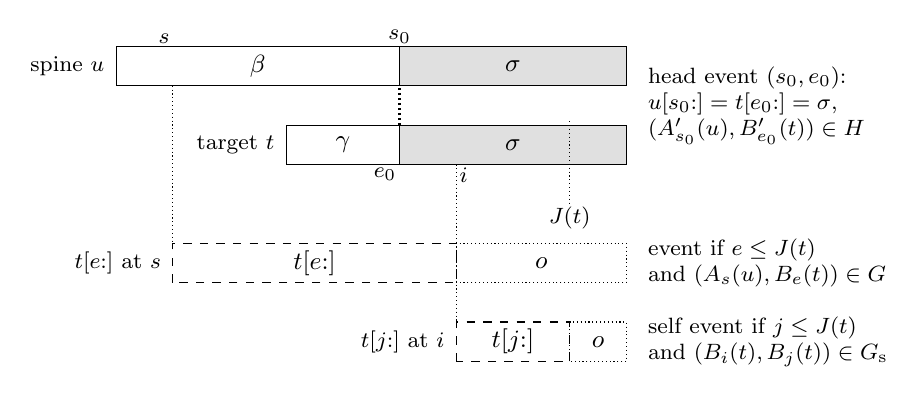
\begin{tikzpicture}[>=Stealth,font=\small,x=0.72cm,y=1cm,
    every node/.style={inner sep=1.5pt},
    box/.style={draw,minimum height=0.5cm,inner sep=0pt},
    lb/.style={font=\footnotesize,inner sep=1pt},
    side/.style={font=\footnotesize,anchor=west,align=left}]
  % spine u = beta sigma and target t = gamma sigma, aligned at their ends
  \draw (0,2.75) rectangle node{$\beta$} (5,3.25);
  \draw[fill=black!12] (5,2.75) rectangle node{$\sigma$} (9,3.25);
  \node[lb,anchor=east] at (-0.15,3) {spine $u$};
  \draw (3,1.75) rectangle node{$\gamma$} (5,2.25);
  \draw[fill=black!12] (5,1.75) rectangle node{$\sigma$} (9,2.25);
  \node[lb,anchor=east] at (2.85,2) {target $t$};
  \node[lb,anchor=south] at (5,3.25) {$s_0$};
  \node[lb,anchor=north east] at (5,1.75) {$e_0$};
  \draw[densely dotted,thick] (5,2.25) -- (5,2.75);
  \draw[densely dotted] (8,2.3) -- (8,1.25);
  \node[lb,anchor=north] at (8,1.25) {$J(t)$};
  \node[side] at (9.3,2.5) {head event $(s_0,e_0)$:\\
    $\wsuf u{s_0}=\wsuf t{e_0}=\sigma$,\\ $(A'_{s_0}(u),B'_{e_0}(t))\in\Head$};
  % a cross comparison (s,e): t[e:] placed at the cut s of u
  \draw[box,dashed] (1,0.25) rectangle node{$\wsuf te$} (6,0.75);
  \draw[densely dotted] (6,0.25) rectangle node{$o$} (9,0.75);
  \draw[densely dotted] (1,2.75) -- (1,0.75);
  \node[lb,anchor=south east] at (1,3.25) {$s$};
  \node[lb,anchor=east] at (0.85,0.5) {$\wsuf te$ at $s$};
  \node[side] at (9.3,0.5) {event if $e\le J(t)$\\ and $(A_s(u),B_e(t))\in\Guard$};
  % a self comparison (i,j): t[j:] placed at the cut i of t
  \draw[box,dashed] (6,-0.75) rectangle node{$\wsuf tj$} (8,-0.25);
  \draw[densely dotted] (8,-0.75) rectangle node{$o$} (9,-0.25);
  \draw[densely dotted] (6,1.75) -- (6,-0.25);
  \node[lb,anchor=north west] at (6,1.75) {$i$};
  \node[lb,anchor=east] at (5.85,-0.5) {$\wsuf tj$ at $i$};
  \node[side] at (9.3,-0.5) {self event if $j\le J(t)$\\ and $(B_i(t),B_j(t))\in\GuardS$};
\end{tikzpicture}
\caption{The pairs of cuts that decide whether $(u,t)$ is a hole
(\cref{def:ex-ss2self,def:ex-events}). Top: the spine and the target, aligned
at their ends; a head event $(s_0,e_0)$ splits them into the heads $\beta$ and
$\gamma$ and the common suffix $\sigma$ (shaded). Middle: a cross comparison
$(s,e)$ places $\wsuf te$ at the cut $s$ of $u$, where it must be a prefix of
$\wsuf us$, leaving the overhang $o$. Bottom: a self comparison $(i,j)$ places
$\wsuf tj$ at the cut $i$ of $t$ in the same way. A hole needs a head event,
a safe spine and a first rejected cut $J(t)$ of the target, and it must have
no event and no self event: every cross comparison $(s,e)$ with $e\le J(t)$
must carry a state pair outside the guard $\Guard$, and every self comparison
$(i,j)$ with $j\le J(t)$ a pair outside the self guard $\GuardS$.}
\Description{Two bars at the top, the spine u and below it the shorter target
t, aligned at the right. The spine consists of beta and the shaded common
suffix sigma, the target of gamma and sigma; a dotted line joins the cuts s
zero and e zero, where sigma begins, and is labeled as the head event. A
dotted line marks the first rejected cut J of t. Below, a dashed box holding
the suffix of t from the cut e starts at the cut s of the spine and is
followed by the overhang o; it is labeled event if e is at most J and the
guard holds. At the bottom, a dashed box holding the suffix of t from the cut
j starts at the cut i of the target and is followed by the overhang o; it is
labeled self event if j is at most J and the self guard holds.}
\label{fig:ex-hole}
\end{figure}


\begin{definition}[Forced target heads]\label{def:ex-fh}
An instance $I$ has \emph{forced target heads}, condition \emph{(FH)}, if for
every $(r,r')\in\Head$ with $r$ reachable in $A'$ and every word $\gamma$ with
$B'(\gamma)=r'$, no proper prefix of $\gamma$ is rejected:
$B_i(\gamma)\notin\Rej$ for all $i<\len\gamma$.
\end{definition}

\begin{lemma}[Heads end before the first rejected cut]\label{lem:ex-head-before-J}
Let $I$ satisfy (FH), and let $(s,e)$ be a head event of $(u,t)$, where $J(t)$
is defined. Then $e\le J(t)$: the target head ends at or before the first
rejected cut, and $\wsuf t{J(t)}$ is a suffix of the common suffix.
\end{lemma}

\begin{proof}
The state $A'_s(u)$ is reachable, and $B'(\wpre te)=B'_e(t)$ is paired with
it by $\Head$. By (FH), $B_i(t)=B_i(\wpre te)\notin\Rej$ for every $i<e$, so the
first rejected cut is at least $e$.
\end{proof}

\Cref{sec:nm} uses \cref{lem:ex-head-before-J} to split a hole at its first
rejected cut. In the extracted instances, (FH) holds by construction
(\cref{lem:ex-fh}).

\subsection{The Extracted Instances}\label{sec:ex-instances}

The instance for a pair of visible signed variables $p,q\in X^\pm$ tests a
pure derivation of $\psi$ from a seed $(p,t)$ to an atom $(q,u)$. The names
follow the readers of \citet{Zhao26}: the \emph{target} is the word whose rejection
is tested, here the seed word $t$, read by the source automaton $\Bsrc_p$ of
\cref{sec:un}; the \emph{spine} is the word $u$ of the derived atom. The
derivation therefore runs from the target to the spine.

\begin{definition}[Extracted instance]\label{def:ex-instance}
For $p,q\in X^\pm$, the \emph{extracted instance}
$I_{pq}=I_{pq}(\varphi,\psi)$ consists of:
\begin{itemize}[leftmargin=*]
\item $A$, the lower automaton of $q$ in $\varphi$, with
  $\Bad=\{Q:Q\cap\Fup\varphi\ne\varnothing\}$;
\item $B=\Bsrc_p$, the source automaton of $p$ (\cref{def:un-source}), with
  \[
   \Rej=\{\zeta:\ \mathrm{dt}(\zeta)\text{ and }\mathrm{du}(\zeta)\text{ both
   fail}\};
  \]
\item $\Guard=\{(Q,(P,b,P')):Q\cap P\ne\varnothing\}$, and $\GuardS$ the self
  guard of \cref{def:un-source};
\item $A'$, the lower automaton of $q$ in $\psi$, and $B'$, the upper
  automaton of $p$ in $\psi$, with $\Head=\{(Q',P'):Q'\cap P'\ne\varnothing\}$.
\end{itemize}
The start states $\downc\varphi q$, the start state of $\Bsrc_p$,
$\downc\psi q$, and $\upc\psi p$ are renamed $0$.
\end{definition}

\begin{table}[tbp]
\caption{The extracted instance $I_{pq}$ for a seed $(p,t)$ and a derived atom
$(q,u)$. The state of $B$ at a cut $e$ of $t$ is
$(P^\varphi_{p,e}(t),[(\bar p,\wpre te)\in\mu_\varphi],P^\psi_{p,e}(t))$, by
\cref{lem:un-source}.}
\label{tab:ex-instance}
\centering
\small
\begin{tabular}{@{}lll@{}}
\toprule
Part & Reads & Meaning\\
\midrule
$A$, $\Bad$ & $Q^\varphi_{q,s}(u)$ on the spine $u$ &
  safe spine: $(q,u)\notin\mu_\varphi$ (\cref{lem:sm-mu})\\
$B$, $\Rej$ & the source automaton on the target $t$ &
  rejected: $\neg\DeadT_\varphi(p,\wpre te)$ and $\neg\DeadU_\psi(p,\wpre te)$\\
$\Guard$ & $Q^\varphi_{q,s}(u)\cap P^\varphi_{p,e}(t)$ &
  event: $(q,u)\in \Reach_\varphi(p,t)$ (\cref{lem:sm-membership})\\
$\GuardS$ & $P^\varphi_{p,i}(t)\cap\overline{P^\varphi_{p,j}(t)}$ &
  self event: $(p,t)$ is dead (\cref{thm:sm-dead})\\
$A'$, $B'$, $\Head$ & $Q^\psi_{q,s}(u)\cap P^\psi_{p,e}(t)$ &
  head event: $(p,t)\to^*_\psi(q,u)$ (\cref{lem:sm-lowest-point})\\
\bottomrule
\end{tabular}
\end{table}

\Cref{tab:ex-instance} summarizes the instance. The automata have
$N_A=2^{2\len X}$, $N_B=2^{4\len X+2\len Z+1}$, and
$N_{A'}=N_{B'}=2^{2(\len X+\len Z)}$ states, and the $4\len X^2$ instances are
computable from $\varphi$ and $\psi$.

Rejection is enriched: a cut of the seed is rejected only if it is neither
dead by support in $\varphi$ nor root-dead in $\psi$. Both properties are
inherited by prefixes (\cref{lem:sm-roots}(4), \cref{lem:sm-dead-states}(4)),
so a rejected cut stays rejected on every extension: $J(t)$ is defined iff $t$
itself is rejected, that is, iff neither $\DeadT_\varphi(p,t)$ nor
$\DeadU_\psi(p,t)$ holds.

\begin{lemma}[Forced target heads]\label{lem:ex-fh}
Every extracted instance $I_{pq}$ satisfies (FH). No hypothesis on $\varphi$
or $\psi$ is needed.
\end{lemma}

\begin{proof}
Let $(Q',P')\in\Head$ and $B'(\gamma)=P'$. Then
$P^\psi_p(\gamma)=P'\ne\varnothing$, and by \cref{lem:sm-head-prefix},
$\DeadU_\psi(p,\wpre\gamma i)$ for every $i<\len\gamma$. By
\cref{lem:un-source}(2), $\mathrm{du}$ holds at every such cut, so
$B_i(\gamma)\notin\Rej$.
\end{proof}

Without the enrichment, that is, with $\Rej$ defined by the failure of
$\mathrm{dt}$ alone, the target head can extend beyond the first rejected cut
(\cref{ex:ex-arrow}).

\subsection{Holes and Condition (II)}\label{sec:ex-reduction}

\begin{theorem}[Holes and condition (II)]\label{thm:ex-reduction}
Let $\varphi$ be satisfiable, let \CondU\ hold, let $p,q\in X^\pm$, and let
$u,t$ be words. Then $(u,t)$ is a hole of $I_{pq}$ iff $(p,t)$ is live in
$\varphi$, $(p,t)\to^*_\psi(q,u)$, and $(q,u)\notin\Cl_\varphi(p,t)$.
Consequently:
\begin{enumerate}[leftmargin=*]
\item condition \CondII\ holds iff no extracted instance $I_{pq}$ has a hole;
\item for every hole $(u,t)$ of $I_{pq}$, the least model $\Cl_\varphi(p,t)$
  of $\varphi$ that contains $(p,t)$ is not the restriction to $X$ of any
  model of $\psi$, so its solution has no extension to a solution of $\psi$.
\end{enumerate}
\end{theorem}

The conditions of \cref{def:ex-ss2self} match the three requirements one by
one. A head event is the lowest point of the pure derivation of $\psi$. A safe
spine and the absence of events say that $(q,u)$ lies neither in $\mu_\varphi$
nor in $\Reach_\varphi(p,t)$ (\cref{lem:sm-membership}). A rejected target and the
absence of self events say that $(p,t)$ is neither dead by support nor has a
self event, that is, that it is live (\cref{thm:sm-dead}). Here \CondU\ is used:
a live seed must also be rejected, which requires that it not be root-dead in
$\psi$. The bounds $e\le J(t)$ and $j\le J(t)$ in \cref{def:ex-ss2self} lose
nothing: the guards require a nonempty set $P^\varphi_{p,e}(t)$, and the pop bound
(\cref{lem:sm-roots}(2)) empties these sets after $J(t)$. The proof is in
\cref{app:sm}.

\begin{corollary}[Entailment and holes]\label{cor:ex-entailment}
Let $\varphi$ and $\psi$ be satisfiable. Then $\varphi\models\Exists\psi$ iff
condition \CondI\ holds, condition \CondU\ holds, and no extracted instance
$I_{pq}$ with $p,q\in X^\pm$ has a hole.
\end{corollary}

\begin{proof}
If \CondU\ fails, the entailment fails by \cref{thm:ch-characterization}.
Otherwise, by \cref{thm:ch-characterization}, the entailment holds iff \CondI\
and \CondII\ hold, and by \cref{thm:ex-reduction}(1), \CondII\ holds iff no
$I_{pq}$ has a hole.
\end{proof}

Conditions \CondI\ and \CondU\ are decidable
(\cref{prop:sm-decide,thm:un-decidable}), and every extracted instance
satisfies (FH) (\cref{lem:ex-fh}). It remains to decide the hole problem for
instances with forced target heads, which \cref{sec:nm,sec:mo} do.

\begin{example}[Condition (U) cannot be dropped]\label{ex:ex-u-needed}
Without \CondU, a failure of \CondII\ need not be a hole. Let $\varphi$ be
empty over $X=\{x,y\}$, and let $\psi=\{x\le y,\ x\le f(a,b)\}$ with $a,b$
hidden and $f$ binary and covariant. The seed $(x^0,\eps)$ is live in
$\varphi$, the copy $(x^0,\eps)\to(y^0,\eps)$ is a pure move of $\psi$, and
$(y^0,\eps)\notin\Cl_\varphi(x^0,\eps)$, so \CondII\ fails at this seed. But
$x^0$ is the root of the upper constructor literal $x^0\le f(a^0,b^0)$ of
$\psi^\pm$, so $\DeadU_\psi(x^0,\eps)$ holds and the target $\eps$ of
$I_{x^0y^0}$ is not rejected: $(\eps,\eps)$ is not a hole. Here \CondU\ fails,
with the countermodel $x=\Top$. The enrichment trades \CondU\ for (FH): with
the rejection test given by the failure of $\mathrm{dt}$ alone, the holes still
characterize the failures of \CondII\ when $\varphi$ is satisfiable, without
assuming \CondU, but (FH) can fail (\cref{ex:ex-arrow}).
\end{example}

\begin{remark}[Covariant and joint-parity instances]\label{rem:ex-covariant}
Informally, if $\varphi$ has a parity assignment (\cref{rem:ch-parity}), in
particular if $f$ is covariant, the self guard never applies to reachable
states of the target automaton (\cref{rem:sm-parity}), and the extracted
instances behave like instances of the suffix-sharing two-word problem
without self events.
\end{remark}

\begin{example}[Shift closure: a hole]\label{ex:ex-running}
Continue \cref{ex:un-running} with $\psi=\{x\le z,\ z\le y,\ z\le f(z,z)\}$ and
$\varphi'_1=\{x\le y,\ y\le g,\ g\le f(g,g)\}$, both satisfiable. Condition
\CondU\ holds, and \CondI\ holds because $\psi$ has no facts.
Consider the seed variable $y^1$ and the derived variable $x^1$. The copy and
constructor literals of $(\varphi'_1)^\pm$ are $x^0\le y^0$, $y^0\le g^0$,
$g^0\le f(g^0,g^0)$, $y^1\le x^1$, $g^1\le y^1$, and $f(g^1,g^1)\le g^1$. In
$I_{y^1x^1}$:
\begin{itemize}[leftmargin=*]
\item $A$ starts at $\downc{\varphi'_1}x^1=\{x^1,y^1,g^1\}$ and moves to
  $\{g^1\}$ on every letter; $\varphi'_1$ has no facts, so every spine
  is safe; the state $\{g^1\}$ lies on a loop at which both letters are safe,
  so it is \emph{branching} (\cref{def:nm-kinds}), the case in which
  \cref{sec:nm} completes every pre-hole directly (\cref{lem:nm-breaker});
\item $P^{\varphi'_1}_{y^1}$ is $\{y^1,x^1\}$ at the empty word and empty
  afterwards, $\mu_{\varphi'_1}=\varnothing$, and $\DeadT^\eps_{\varphi'_1}=
  \{x^0,y^0,g^0\}$; with \cref{ex:un-running}, no cut of any target is dead by
  support or root-dead, so $J(t)=0$ for every target $t$;
\item hence the only possible event is $(0,0)$, a cross comparison iff
  $t\pre u$, and there are no self events, since
  $P^{\varphi'_1}_{y^1,j}(t)=\varnothing$ for $j\ge1$;
\item $Q^\psi_{x^1}(\beta)$ always meets $\upc\psi y^1=\{y^1,z^1,x^1\}$, and
  $P^\psi_{y^1}(\gamma)=\varnothing$ for $\gamma\ne\eps$, so the head events
  are the pairs $(s,0)$ with $\wsuf us=t$.
\end{itemize}
So the holes of $I_{y^1x^1}$ are the pairs $(u,t)$ in which $t$ is a suffix but
not a prefix of $u$, for example $(01,1)$, with head event $(1,0)$. By
\cref{thm:ex-reduction}, $\psi$ derives $(x^1,01)$ from the live seed
$(y^1,1)$, and $(x^1,01)\notin\Cl_{\varphi'_1}(y^1,1)$. In words: if $y$ has a
leaf $\Bot$ at a prefix of $1$, then every $z$ between $x$ and $y$ with
$z\le f(z,z)$ has a leaf $\Bot$ at a prefix of $1$ and hence at a prefix of
$01$, and so does $x$. A finite countermodel is
$x=y=f(f(\Bot,f(\Bot,\Bot)),\Bot)$, whose constructor positions are $\eps$,
$0$, and $01$, with $g$ the complete binary tree whose constructor positions
are the words of length at most $2$. The least model $\Cl_{\varphi'_1}(y^1,1)$
of \cref{thm:ex-reduction}(2) is the solution $x=y=f(\Omega,\Bot)$ and
$g=\Omega$. Since $J(t)=0$, the target head is empty, and (FH) holds trivially
for this instance.
\end{example}

\begin{example}[A target head beyond the cuts dead by support]\label{ex:ex-arrow}
Continue \cref{ex:un-arrow} with $\varphi=\{x\le x\to x\}$ and
$\psi=\{x\le a\to x,\ c\to y\le a\}$, both satisfiable: $x=\Bot$ solves
$\varphi$, and $x=y=\Bot$, $a=c=\Top$ solve $\psi$. Conditions \CondI\ and
\CondU\ hold. Consider the seed variable $x^0$, the derived variable $y^1$,
and the pair $(u,t)=(\eps,01)$ in $I_{x^0y^1}$. Along the target $t=01$, the
upper automata give
\[
 P^\varphi_{x^0}:\ \{x^0\},\ \{x^1\},\ \varnothing,\qquad
 P^\psi_{x^0}:\ \{x^0\},\ \{a^1\},\ \{y^1\}
\]
at the cuts $0,1,2$. With $\DeadT^\eps_\varphi=\{x^0\}$ and
$\DeadU^\eps_\psi=\{x^0,a^1\}$, cut $0$ is dead by support, cut $1$ is not dead
by support but root-dead in $\psi$, and cut $2$ is rejected: $J(01)=2$. The
head event is $(0,2)$, since $Q^\psi_{y^1}(\eps)=\{y^1\}=P^\psi_{x^0}(01)$: the
derivation pops $0$ from $x^0$ to $a^1$ and then $1$ from $a^1$ to $y^1$. The
only cross comparison $(s,e)$ with $e\le2$ is $(0,2)$, whose guard
$\{y^1\}\cap P^\varphi_{x^0}(01)$ is empty; the self comparisons of $01$ ending
at $2$ have an empty self guard, and $(0,1)$ is not a self comparison. The
spine is safe because $\varphi$ has no facts. So $(\eps,01)$ is a
hole: $\psi$ derives $(y^1,\eps)$, that is $y=\Bot$, from the live seed
$(x^0,01)$. A countermodel is $x=(\Bot\to\Bot)\to\Bot$ and $y=\Top$: from
$x\le a\to x$ and $c\to y\le a$, any extension would have
$c\to\Top\le_c a\le_c\Bot\to\Bot$, hence $\Top\le_c\Bot$.

The target head is $\gamma=01$. The rejection test given by the failure of
$\mathrm{dt}$ alone would reject already at cut $1$, inside the head: $(x^0,0)$
is not dead by support, although it is dead by the self event $(0,1)$ of the
word $0$ (\cref{ex:sm-arrow}). So the unenriched instance does not satisfy
(FH). The enrichment rejects only at cut $2$, because $(x^0,0)$ is root-dead
in $\psi$.
\end{example}

%% nonmortal -- holes of the two-word problem with self events that are not
%% mortal: the continuation identity, the decomposition at the first rejected
%% cut, kinds of state, the breaker, lassos, short pre-holes, aperiodic
%% lassos, the pump for periodic lassos, and the three-case theorem.
%% Full proofs are in appendix-nonmortal.tex.

\section{Non-Mortal Holes}\label{sec:nm}

Let $I$ be an instance of the two-word hole problem with self events
(\cref{def:ex-ss2self}) that satisfies condition (FH) (\cref{def:ex-fh}). This section shows that if
$I$ has a hole, then it has a hole whose length is polynomial in the sizes of
its four automata, or it has a \emph{mortal hole}: a hole $(u,t)$ whose spine
ends in a state without infinite safe continuations and whose target ends
fewer than $N_A$ letters after its first rejected cut
(\cref{thm:nm-three-cases}). Mortal holes are treated in \cref{sec:mo}.

The argument starts from a simple observation. Cutting a hole $(u,t)$ at the
first rejected cut $J(t)$ of its target splits off the \emph{continuation}
$\theta=\wsuf t{J(t)}$. Condition (FH) places every target head before $J(t)$,
so $\theta$ is a common suffix of both words, and what remains is a shorter
pair $(u_0,t_0)$ with $u=u_0\theta$ and $t=t_0\theta$, a \emph{pre-hole}
(\cref{lem:nm-decomposition} and \cref{fig:nm-prehole}). Appending the same
word to both words creates no new events and no new self events, and it keeps
an existing one exactly when it continues the overhang of that event
periodically (\cref{lem:nm-continuation}). The question is therefore whether
a single continuation that keeps the spine automaton out of $\Bad$ can break
every pending obligation of a pre-hole: its events, which are never aligned,
and the self events of its target. The answer depends on the state
$q=A(u_0)$ at the end of the spine of the pre-hole.
\begin{itemize}[leftmargin=*]
\item If a cycle that offers a choice of two letters is reachable from $q$,
  a breaking continuation of length at most $\max(\len{u_0},\len{t_0})+3N_A$
  always exists (\cref{lem:nm-breaker}).
\item If every reachable cycle is forced, then the long continuations follow
  finitely many ultimately periodic words, the \emph{lassos} of $q$
  (\cref{lem:nm-thin}). A lasso that is not purely periodic breaks every
  obligation (\cref{lem:nm-aperiodic}). A purely periodic lasso may let
  obligations survive, and then the pre-hole itself has to be shortened. The
  \emph{pump} (\cref{thm:nm-pump}) deletes factors of the two words while
  keeping the endpoint $q$ and the absence of surviving obligations, down to a
  length polynomial in the sizes of the automata.
\item In the remaining cases the continuation reaches a state without
  infinite safe continuations within fewer than $N_A$ letters, and the hole is
  mortal.
\end{itemize}

\paragraph{Conventions}
We use the instance, safety, comparison, event, and forced-head conventions of
\cref{def:ex-ss2self,def:ex-events,def:ex-fh}. For an automaton $M$, let
$M(r,w)$ denote its state after reading $w$ from $r$, and let
$M_s(w)=M(0,\wpre ws)$ be its state at the cut $s$ of $w$. We abbreviate the
state counts as
\[
 a=N_A,\qquad b=N_B,\qquad a'=N_{A'},\qquad b'=N_{B'};
\]
all four are at least $1$.

An \emph{infinite word} $\xi'=\xi'[0]\xi'[1]\cdots$ over $\Sigma$ has prefixes
$\wpre{\xi'}k$ and suffixes $\wsuf{\xi'}k$ as for finite words, and $v\xi'$ is the
infinite word that starts with the finite word $v$. A number $\varpi\ge1$ is a
\emph{period} of $\xi'$ if $\xi'[i+\varpi]=\xi'[i]$ for all $i\ge0$; $\xi'$ is \emph{purely
periodic} if it has a period, and its \emph{least period} is then the least of
its periods. For a nonempty finite word $o$, $o^\omega=ooo\cdots$ is the
infinite word with period $\len o$ that begins with $o$; a finite word is a
prefix of $o^\omega$ exactly when it is a prefix of some $o^k$, in agreement
with the notation $\theta\pre o^\omega$ of \cref{sec:bg-words}. Holes are
written $(u,t)$, pre-holes $(u_0,t_0)$, continuations $\theta$, and infinite
words $\xi$.

\subsection{The Continuation Identity}\label{sec:nm-continuation}

For a cross comparison $(s,e)$ of $(u,t)$ and a word $\theta$, we say that
$\theta$ \emph{keeps} $(s,e)$ if $\wsuf te\,\theta\pre\wsuf us\,\theta$, and
that $\theta$ \emph{breaks} it otherwise; for a self comparison $(i,j)$ of $t$,
$\theta$ keeps it if $\wsuf tj\,\theta\pre\wsuf ti\,\theta$. Non-aligned cross
comparisons can be unboundedly many: if $u=\ell^k$ and $t=\ell^m$ for a letter
$\ell$, every pair of cuts with a nonnegative offset is one. We therefore do
not count them but control them through common continuations.

\begin{lemma}[Continuation identity]\label{lem:nm-continuation}
Let $u$, $t$ and $\theta$ be words such that $J(t)$ is defined.
\begin{enumerate}[label=(\alph*)]
\item $J(t\theta)=J(t)$, and each of the four automata has the same state at
every cut $s\le\len u$ of $u\theta$ as at the cut $s$ of $u$, and at every cut
$e\le\len t$ of $t\theta$ as at the cut $e$ of $t$.
\item Let $s\le\len{u\theta}$ and $e\le J(t)$. Then $(s,e)$ is a cross
comparison of $(u\theta,t\theta)$ if and only if $s\le\len u$, $(s,e)$ is a
cross comparison of $(u,t)$, and $\theta$ keeps it. Likewise, for
$i<j\le J(t)$, the pair $(i,j)$ is a self comparison of $t\theta$ if and only
if it is a self comparison of $t$ and $\theta$ keeps it.
\item A word $\theta$ keeps a cross or self comparison with overhang $o$ if and
only if $\theta\pre o\theta$. If $o\ne\eps$, this holds if and only if
$\theta\pre o^\omega$. Every word keeps every aligned cross comparison.
\end{enumerate}
\end{lemma}

In words: a common continuation creates no new comparison among the cuts up to
$J(t)$, and it keeps an existing one exactly when it continues the overhang
periodically. The proof is in \cref{app:nm-continuation}. We use the lemma
through the following \emph{continuation facts}, which hold for all words $u$
and $t$ with $J(t)$ defined and every word $\theta$:
\begin{enumerate}[label=(K\arabic*)]
\item the events of $(u\theta,t\theta)$ are exactly the events of $(u,t)$ that
$\theta$ keeps, and the self events of $t\theta$ are exactly the self events of
$t$ that $\theta$ keeps;
\item every word keeps every aligned cross comparison, so aligned events can
never be removed;
\item if $\theta$ breaks a cross or self comparison, so does every word with
prefix $\theta$;
\item every head event of $(u,t)$ is a head event of $(u\theta,t\theta)$;
\item if $u$ is safe, then $u\theta$ is safe if and only if $\theta$ is safe
from $A(u)$.
\end{enumerate}
A non-aligned event or a self event with overhang $o$ is thus a periodicity
obligation: a continuation removes it exactly when it departs from $o^\omega$.

\subsection{Pre-Holes and the Decomposition at the First Rejected Cut}\label{sec:nm-prehole}

\begin{definition}[Pre-hole]\label{def:nm-prehole}
A \emph{pre-hole} of $I$ is a pair $(u_0,t_0)$ such that $u_0$ is safe,
$J(t_0)=\len{t_0}$, $(u_0,t_0)$ has a head event, and $(u_0,t_0)$ has no aligned
event. Its \emph{obligations} are its events and the self events of $t_0$. A
word $\theta$ \emph{completes} $(u_0,t_0)$ if $\theta$ is safe from $A(u_0)$ and
breaks every obligation of $(u_0,t_0)$.
\end{definition}

No obligation of a pre-hole is aligned, so every obligation has a nonempty
overhang. The overhang of an event has length at most $\len{u_0}$ and that of a
self event at most $\len{t_0}$, so every obligation has an overhang of length at
most
\[
 W=\max(\len{u_0},\len{t_0}).
\]
A pre-hole without obligations is a hole, completed by the empty word.

\begin{figure}[t]
\centering
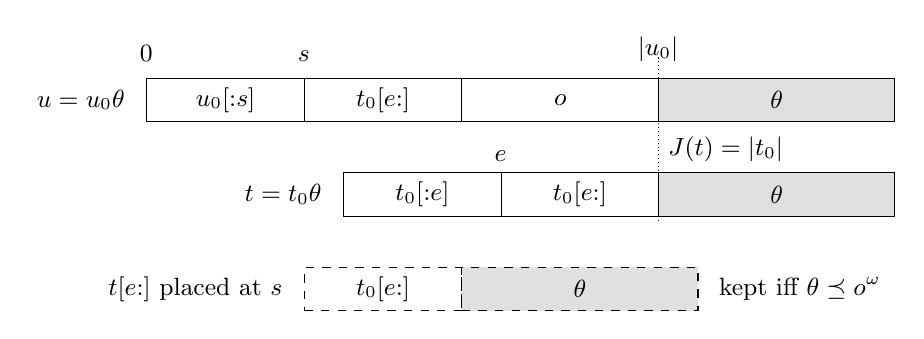
\begin{tikzpicture}[x=1cm,y=1.2cm,font=\small,
  box/.style={draw,minimum height=0.55cm,inner sep=0pt},
  cont/.style={box,fill=black!12},
  shifted/.style={box,dashed}]
  % spine u = u_0 theta
  \node[box,minimum width=2.0cm,anchor=west] at (0,2) {$\wpre{u_0}{s}$};
  \node[box,minimum width=2.0cm,anchor=west] at (2,2) {$\wsuf{t_0}{e}$};
  \node[box,minimum width=2.5cm,anchor=west] at (4,2) {$o$};
  \node[cont,minimum width=3.0cm,anchor=west] at (6.5,2) {$\theta$};
  \node[anchor=east] at (-0.15,2) {$u=u_0\theta$};
  % target t = t_0 theta
  \node[box,minimum width=2.0cm,anchor=west] at (2.5,1) {$\wpre{t_0}{e}$};
  \node[box,minimum width=2.0cm,anchor=west] at (4.5,1) {$\wsuf{t_0}{e}$};
  \node[cont,minimum width=3.0cm,anchor=west] at (6.5,1) {$\theta$};
  \node[anchor=east] at (2.35,1) {$t=t_0\theta$};
  % the target suffix t[e:] = t_0[e:] theta placed at the cut s of u
  \node[shifted,minimum width=2.0cm,anchor=west] at (2,0) {$\wsuf{t_0}{e}$};
  \node[shifted,fill=black!12,minimum width=3.0cm,anchor=west] at (4,0) {$\theta$};
  \node[anchor=east] at (1.85,0) {$\wsuf te$ placed at $s$};
  \node[anchor=west] at (7.15,0) {kept iff $\theta\pre o^\omega$};
  % cuts
  \draw[densely dotted] (6.5,2.45) -- (6.5,0.72);
  \node[above] at (0,2.3) {$0$};
  \node[above] at (2,2.3) {$s$};
  \node[above] at (6.5,2.3) {$\len{u_0}$};
  \node[above,inner sep=2pt] at (4.5,1.28) {$e$};
  \node[above right,inner sep=2pt] at (6.55,1.28) {$J(t)=\len{t_0}$};
\end{tikzpicture}
\Description{Three rows of boxes. The top row is the spine, divided into
the prefix of the pre-hole spine before the cut s, a copy of the target
suffix from cut e, the overhang o, and the shaded continuation theta. The
middle row is the target, right-aligned with the spine, divided into the
target prefix before e, the target suffix from e, and the shaded
continuation theta; a dotted line marks the first rejected cut. The bottom
row places the target suffix and theta at the cut s of the spine, so that
theta lies below the overhang.}
\caption{A hole $(u,t)=(u_0\theta,t_0\theta)$ cut at the first rejected cut
$J(t)=\len{t_0}$ of its target (\cref{lem:nm-decomposition}); the continuation
$\theta$ is shaded. An event $(s,e)$ of the pre-hole $(u_0,t_0)$ places
$\wsuf{t_0}e$ at the cut $s$ of $u_0$, followed by the overhang $o=o(s,e)$.
After $\theta$ is appended, $(s,e)$ is still a cross comparison if and only if
the shifted copy of $\theta$ (bottom row) agrees with $o\theta$, that is, if
and only if $\theta\pre o^\omega$ (\cref{lem:nm-continuation}). A self event
$(i,j)$ of $t_0$ behaves in the same way, with $t_0$ in the top row. A hole
requires $\theta$ to break every event and every self event.}
\label{fig:nm-prehole}
\end{figure}

\begin{lemma}[Decomposition at the first rejected cut]\label{lem:nm-decomposition}
If $(u_0,t_0)$ is a pre-hole and $\theta$ completes it, then
$(u_0\theta,t_0\theta)$ is a hole. Conversely, let $I$ satisfy \textup{(FH)} and
let $(u,t)$ be a hole. Then $\theta=\wsuf t{J(t)}$ is a suffix of $u$, and if
$u=u_0\theta$ and $t=t_0\theta$, then $(u_0,t_0)$ is a pre-hole and $\theta$
completes it.
\end{lemma}

In one direction, appending a completing word keeps the spine safe, keeps the
head event, and leaves no event and no self event, by (K5), (K4) and (K1). In
the other, (FH) places the target head of a head event before $J(t)$
(\cref{lem:ex-head-before-J}). Hence
$\theta$ is no longer than the common suffix and can be split off both words,
and (K1) and (K2) show that $\theta$ breaks every obligation of $(u_0,t_0)$ and
that $(u_0,t_0)$ has no aligned event. The proof is in
\cref{app:nm-continuation}. Condition (FH) cannot be dropped
(\cref{ex:nm-fh}).

\begin{example}[Shift closure: decomposition]\label{ex:nm-running}
In the instance $I_{y^1x^1}$ of \cref{ex:ex-running}, every target $t$ has
$J(t)=0$. So the hole $(01,1)$ splits as $\theta=\wsuf t0=1$ and
$(u_0,t_0)=(0,\eps)$. The pre-hole $(0,\eps)$ has the head event $(1,0)$,
and this aligned pair is not an event, because $A_1(0)=\{g^1\}$ misses
$P^{\varphi'_1}_{y^1}(\eps)=\{y^1,x^1\}$. Its only obligation is the event
$(0,0)$, with overhang $0$; the target $\eps$ has no self comparison. By
\cref{lem:nm-continuation}(c), a continuation keeps this obligation iff it is a
prefix of $0^\omega$. So the continuation $0$ keeps it, and indeed $(00,0)$
has the event $(0,0)$, while every continuation that contains the letter $1$
breaks it; the shortest one, $\theta=1$, gives back the hole $(01,1)$.
\end{example}

\subsection{Kinds of State}\label{sec:nm-kinds}

Let $\mathcal G_A$ be the \emph{safe graph} of $A$: its vertices are the safe
states of $A$, with an edge from $r$ to $A(r,\ell)$, labeled by the letter
$\ell$, whenever $A(r,\ell)$ is safe. The labels of the paths from $r$ are
exactly the words safe from $r$. A safe state is \emph{cyclic} if it lies on a
cycle of $\mathcal G_A$, and a letter $\ell$ is \emph{safe at} a safe state $r$
if $A(r,\ell)$ is safe.

\begin{definition}[Kinds of state]\label{def:nm-kinds}
A safe state $q$ of $A$ is
\begin{itemize}
\item \emph{mortal} if no infinite word is safe from $q$, equivalently, if no
cyclic state is reachable from $q$ in $\mathcal G_A$;
\item \emph{branching} if some cyclic state $r$ reachable from $q$ in
$\mathcal G_A$ has two distinct safe letters $\ell\ne\ell'$;
\item \emph{thin} if it is neither mortal nor branching.
\end{itemize}
\end{definition}

From a mortal state every safe run dies within $N_A$ letters. From a branching
state some reachable cycle offers a choice of letters, so a safe continuation
can depart from any given period. From a thin state infinite safe runs exist,
but once they reach a cycle they are forced, letter by letter. The two
descriptions of mortality agree because an infinite path in the finite graph
$\mathcal G_A$ repeats a vertex, and a reachable cyclic state can be visited
forever. A branching state reaches a cyclic state, so it is not mortal; the
three kinds are therefore pairwise disjoint, and every safe state has exactly
one of them. Each kind is decided by reachability in $\mathcal G_A$.

Branching asks only for two distinct safe letters at a reachable cyclic state;
the states they lead to may coincide, and the letter that leaves the cycle
need not admit any further safe continuation, since the breaker stops right
after it. Requiring all letters, or two specific letters, to be safe would
misclassify states over larger alphabets. For instance, for arity $n\le1$ no
state has two distinct safe letters, and for $n=0$ there are no letters at
all.

\subsection{The Breaker}\label{sec:nm-breaker}

\begin{lemma}[Breaker]\label{lem:nm-breaker}
Let $q$ be a branching state and $W\ge0$. There is a word $\theta$, safe from
$q$, with $\len\theta\le W+3N_A$, that is not a prefix of $o^\omega$ for any
word $o$ with $1\le\len o\le W$. In particular, every pre-hole $(u_0,t_0)$ with
$A(u_0)$ branching is completed by a word of length at most
$\max(\len{u_0},\len{t_0})+3N_A$.
\end{lemma}

The idea is to steer the spine into a cycle that offers a choice of letters, to
run around it for longer than any overhang, and then to leave it. The word
$\theta=\alpha\lambda^k\ell$ follows a shortest path $\alpha$ to a cyclic state
$r$ with two distinct safe letters, runs $k$ times around a shortest cycle
$\lambda$ through $r$, with $k\len\lambda\ge W+\len\lambda$, and leaves the
cycle by a safe letter $\ell\ne\lambda[0]$; one of the two safe letters at $r$
differs from $\lambda[0]$. If $\theta$ were a prefix of $o^\omega$, then over
the stretch $\lambda^k$, of length at least $\len o+\len\lambda$, it would have
both periods $\len o$ and $\len\lambda$, hence the period
$\gcd(\len o,\len\lambda)$ by the theorem of Fine and Wilf
\citep{FineWilf65}. So after $\lambda^k$ it would have to continue with
$\lambda[0]$, not with $\ell$. This uses only equality of letters and holds
over every alphabet. Every obligation of a pre-hole has a nonempty overhang of
length at most $W=\max(\len{u_0},\len{t_0})$, so $\theta$ breaks it by
\cref{lem:nm-continuation}(c). The proof is in \cref{app:nm-breaker}.

In \cref{ex:nm-running}, the spine state $A(0)=\{g^1\}$ lies on a loop at
which both letters are safe, so it is branching, and the breaker also
completes the pre-hole $(u_0,t_0)=(0,\eps)$. Here $W=1$, and the
construction may take the cyclic state $r=\{g^1\}$ itself, $\alpha=\eps$, the
cycle $\lambda=0$ and $k=2$; this gives $\theta=\alpha\lambda^k\ell=001$ with
the breaker letter $\ell=1$ and the hole $(0001,001)$, while the shortest
completion $\theta=1$ gives back $(01,1)$.

The bound uses $\max(\len{u_0},\len{t_0})$ because the overhang of a self
event of $t_0$ can be as long as $t_0$, which may be longer than $u_0$. The
maximum cannot be replaced by $\len{u_0}$, as the following example shows.

\begin{example}[Self events need the longer word]\label{ex:nm-max}
Let $\Sigma=\{0,1\}$ and $t_0=0001011100$. Let $A$ and $A'$ have a single state
$0$, with $\Bad=\varnothing$, so that $N_A=1$ and the state $0$ of $A$ is
branching, and let $\Guard=\varnothing$. Let $B$ and $B'$ both be the automaton
whose states are the prefixes of $t_0$, with start state $\eps$, and one sink;
it moves from $v$ to $v\ell$ while $v\ell$ is a prefix of $t_0$, and to the
sink otherwise. Let $\Rej=\{t_0\}$, let $\Head$ consist of the pair of the
state of $A'$ and the state $t_0$ of $B'$, and let $\GuardS$ consist of the
pairs $(\wpre{t_0}i,t_0)$ of states of $B$ with $0\le i\le7$. Condition (FH)
holds, since $t_0$ is the only word that leads $B'$ to the state $t_0$, and
its proper prefixes are not rejected. The pair $(\eps,t_0)$ is a pre-hole, and
its obligations are the self events $(i,10)$ with $0\le i\le7$, whose
overhangs are the suffixes $\wsuf{t_0}i$, of length at least $3$. The eight
factors $\wsub{t_0}i{i+3}$, $0\le i\le7$, are the eight words of length $3$
over $\Sigma$. So every word $\theta$ of length at most $3$ is a prefix of some
$\wsuf{t_0}i$ with $i\le7$ and keeps the self event $(i,10)$. Hence no word of
length at most $\len{u_0}+3N_A=3$ completes $(\eps,t_0)$, whereas
\cref{lem:nm-breaker} provides a completion of length at most
$\len{t_0}+3N_A=13$.
\end{example}

\subsection{Thin States and Lassos}\label{sec:nm-thin}

A \emph{lasso} of a safe state $q$ is an infinite word $\alpha\lambda^\omega$
with $\lambda\ne\eps$, $\len\alpha+\len\lambda\le N_A$, $\alpha\lambda$ safe
from $q$, and $A(q,\alpha\lambda)=A(q,\alpha)$. Every lasso of $q$ is safe from
$q$, and there are finitely many.

\begin{lemma}[Thin states]\label{lem:nm-thin}
Let $q$ be a safe state of $A$.
\begin{enumerate}[label=(\alph*)]
\item If $q$ is mortal, every word safe from $q$ has length less than $N_A$
and leads to a mortal state.
\item If $q$ is thin, every cyclic state reachable from $q$ has exactly one
safe letter, and the edge along it leads to a cyclic state.
\item If $q$ is thin, every infinite word safe from $q$ is a lasso of $q$, and
$q$ has at least one lasso.
\item If $q$ is thin, $\theta$ is safe from $q$, and $A(q,\theta)$ is mortal,
then $\len\theta<N_A$.
\end{enumerate}
\end{lemma}

Thus a thin region consists of finitely many lassos together with acyclic
paths into mortal states. Each part follows a safe run until it repeats a
state; the proof is in \cref{app:nm-breaker}.

\begin{definition}[Survival]\label{def:nm-survival}
A cross or self comparison \emph{survives} an infinite word $\xi$ if every
finite prefix of $\xi$ keeps it. An infinite word $\xi$ is
\emph{survivor-free} for a pre-hole $(u_0,t_0)$ if no obligation of
$(u_0,t_0)$ survives $\xi$.
\end{definition}

\begin{lemma}[Survival]\label{lem:nm-survival}
Let $u$ and $t$ be words and $\xi$ an infinite word.
\begin{enumerate}[label=(\alph*)]
\item A cross or self comparison with nonempty overhang $o$ survives $\xi$ if
and only if $\xi=o^\omega$. Every aligned cross comparison survives $\xi$.
\item Let $s\le\len u$ and $e\le\len t$ with $\len t-e\le\len u-s$. Then
$(s,e)$ is a cross comparison of $(u,t)$ that survives $\xi$ if and only if
$\wsuf us\,\xi=\wsuf te\,\xi$. Likewise, for $i<j\le\len t$, the pair $(i,j)$
is a self comparison of $t$ that survives $\xi$ if and only if
$\wsuf ti\,\xi=\wsuf tj\,\xi$.
\item Let $\xi=\alpha\lambda^\omega$ with $\lambda\ne\eps$. If a comparison
with nonempty overhang $o$ does not survive $\xi$, then the prefix of $\xi$ of
length $\len\alpha+\len\lambda+\len o-1$ breaks it.
\end{enumerate}
\end{lemma}

Part (a) is \cref{lem:nm-continuation}(c) applied to every prefix of $\xi$.
Part (b) turns survival into an equality of infinite words, which is the form
used by the pump; it holds because two finite words are prefixes of the same
infinite word exactly when the shorter is a prefix of the longer. Part (c)
compares two ultimately periodic words by the theorem of Fine and Wilf. The
proofs are in \cref{app:nm-survival}.

\begin{corollary}[Lasso completion]\label{cor:nm-lasso-completion}
Let $(u_0,t_0)$ be a pre-hole, and let $\xi$ be a lasso of $A(u_0)$ that is
survivor-free for $(u_0,t_0)$. Then the prefix of $\xi$ of length
$\max(\len{u_0},\len{t_0})+N_A-1$ completes $(u_0,t_0)$.
\end{corollary}

\begin{proof}
The prefix is safe from $A(u_0)$, since $\xi$ is. Write
$\xi=\alpha\lambda^\omega$ with $\len\alpha+\len\lambda\le N_A$. Each
obligation has a nonempty overhang $o$ with $\len o\le\max(\len{u_0},\len{t_0})$
and does not survive $\xi$. By \cref{lem:nm-survival}(c) the prefix of $\xi$ of
length $\len\alpha+\len\lambda+\len o-1\le\max(\len{u_0},\len{t_0})+N_A-1$
breaks it, and by (K3) so does the longer prefix.
\end{proof}

\subsection{Short Pre-Holes}\label{sec:nm-short}

Pre-holes form a recognizable set of pairs. A pre-hole asks for a safe spine,
a target rejected exactly at its end, and conditions on the aligned pairs of
cuts only, and the aligned pairs are the pairs at equal distance from the ends
within the longest common suffix. A finite graph that reads both words
forward, aligned at their right ends, can therefore track the four automata
and two bits: whether some aligned pair seen so far carries $\Head$, and
whether some carries $\Guard$. Both bits are reset whenever the two words
read different letters. Its paths spell exactly the pre-holes, and a shortest
path visits no node twice.

\begin{proposition}[Short pre-holes]\label{prop:nm-short-prehole}
Let $E$ be a set of safe states of $A$. If some pre-hole $(u_0,t_0)$ has
$A(u_0)\in E$, then some pre-hole $(u_1,t_1)$ has $A(u_1)\in E$ and
$\len{u_1},\len{t_1}<12aba'b'$. In particular, it is decidable whether a pre-hole
with $A(u_0)\in E$ exists.
\end{proposition}

The graph has the nodes $(r_A,r_B,r_{A'},r_{B'},h,g,\phi)$, with a state of
each automaton, two bits $h$ and $g$, and a phase $\phi\in\{0,1,2\}$ that
records whether only the spine, only the target, or both words are being read;
hence $12aba'b'$ nodes. The construction and its correctness are in
\cref{app:nm-graph}. The proposition does not preserve survivor-freeness for a
given lasso; it is used where every pre-hole with the given endpoint is good
enough, namely for branching endpoints and for lassos that are not purely
periodic.

\subsection{Aperiodic Lassos}\label{sec:nm-aperiodic}

\begin{lemma}[Aperiodic lassos]\label{lem:nm-aperiodic}
If an infinite word $\xi$ is not purely periodic, then no cross or self
comparison with a nonempty overhang survives $\xi$. In particular, $\xi$ is
survivor-free for every pre-hole.
\end{lemma}

\begin{proof}
By \cref{lem:nm-survival}(a), a comparison with nonempty overhang $o$ survives
$\xi$ only if $\xi=o^\omega$, which is purely periodic. Every obligation of a
pre-hole has a nonempty overhang.
\end{proof}

\subsection{The Pump}\label{sec:nm-pump}

The remaining non-mortal case is a pre-hole whose spine ends in a thin state
$q$ and a purely periodic lasso of $q$ that is survivor-free for it. Here
survivor-freeness depends on the pre-hole, and it can fail for short pre-holes
and hold for long ones, so \cref{prop:nm-short-prehole} does not apply. The
pump shortens the pre-hole directly, keeping its endpoint and its
survivor-freeness. Put
\[
 \Pcap(a,b,a',b')=2aba'b'+a^2a'+ab+aa'+bb' .
\]

\begin{theorem}[Pump]\label{thm:nm-pump}
Let $\xi$ be a purely periodic infinite word with least period $\varpi$, and let
$(u,t)$ be a pre-hole for which $\xi$ is survivor-free. Then there is a
pre-hole $(u',t')$ for which $\xi$ is survivor-free, with $A(u')=A(u)$ and
\[
 \len{u'},\len{t'}<2aba'b'+aa'\varpi+b\varpi+aa'+bb' .
\]
In particular, if $\varpi\le N_A$, then $\len{u'},\len{t'}<\Pcap(a,b,a',b')$.
\end{theorem}

The theorem uses no property of the state $A(u)$, and a lasso enters only
through the bound on its period: if a lasso $\xi=\alpha\lambda^\omega$ is purely
periodic, then its least period is at most $\len\lambda\le N_A$
(\cref{lem:nm-infinite}(b)), so the second bound applies. The proof rests on three
observations and a count; the details are in \cref{app:nm-pump}.

\emph{Survival as an equality of infinite words.} By
\cref{lem:nm-survival}(b), a pre-hole $(u,t)$ is survivor-free for $\xi$ if and
only if no pair of cuts $(s,e)$ with $\len t-e\le\len u-s$ and
$\wsuf us\,\xi=\wsuf te\,\xi$ carries $\Guard$, and no pair of cuts $i<j$ of $t$
with $\wsuf ti\,\xi=\wsuf tj\,\xi$ carries $\GuardS$; the aligned pairs are
among the former. Call such pairs \emph{$\xi$-matched}. The pump only has to
make sure that a deletion creates no new $\xi$-matched pair.

\emph{Rests and periodic ends.} Call a cut $s$ of a word $w$ \emph{periodic}
if $\wsuf ws\,\xi$ has period $\varpi$. The periodic cuts form an interval
$R_w\le s\le\len w$; the factor $\wpre w{R_w}$ is the \emph{rest} of $w$
and $\wsuf w{R_w}$, of length $T_w=\len w-R_w$, its \emph{periodic
end}. The $\xi$-matched pairs have a rigid structure (\cref{fig:nm-ends}). Two
periodic cuts have equal $\xi$-suffixes exactly when their \emph{end
distances}, the distances to the ends of their words, agree modulo $\varpi$. A
periodic cut never matches a rest cut. A rest cut $j$ of $u$ matches at most one cut of $t$, its
\emph{partner}, which is then a rest cut at the same distance before the
boundary of the rest: $R_u-j=R_t-e$. Finally, the infinite word
$\xi'=\wsuf uj\,\xi$ at a rest cut is \emph{non-self-similar}: $z\xi'\ne\xi'$ for every
nonempty finite word $z$. Indeed, $z\xi'=\xi'$ would give $\xi'$ the period $\len z$,
and then also the period $\varpi$ of its suffix $\xi$, which would make $j$ a
periodic cut. Moreover, the periodic end of a target $t$ with $J(t)=\len t$ is
short, $T_t<N_B\,\varpi$ (\cref{lem:nm-target-end}): two of its cuts with the same
state of $B$ and end distances that agree modulo $\varpi$ are followed by the
same letters up to the end of $t$, so the earlier one would lead $B$ to the rejected state
$B(t)$ before the end.

\begin{figure}[t]
\centering
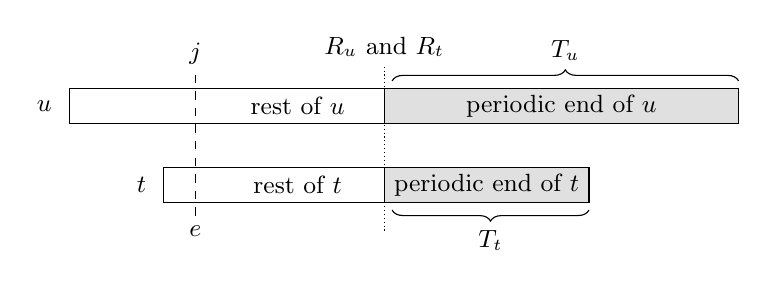
\begin{tikzpicture}[x=1cm,y=1cm,font=\small]
  \draw (1,0.78) rectangle (5,1.22);
  \node at (3.9,1) {rest of $u$};
  \draw[fill=black!12] (5,0.78) rectangle (9.5,1.22);
  \node at (7.25,1) {periodic end of $u$};
  \node[anchor=east] at (0.9,1) {$u$};
  \draw (2.2,-0.22) rectangle (5,0.22);
  \node at (3.9,0) {rest of $t$};
  \draw[fill=black!12] (5,-0.22) rectangle (7.6,0.22);
  \node at (6.3,0) {periodic end of $t$};
  \node[anchor=east] at (2.1,0) {$t$};
  \draw[densely dotted] (5,1.5) -- (5,-0.6);
  \node[above] at (5,1.5) {$R_u$ and $R_t$};
  \draw[dashed] (2.6,1.4) -- (2.6,-0.4);
  \node[above] at (2.6,1.4) {$j$};
  \node[below] at (2.6,-0.4) {$e$};
  \draw[decorate,decoration={brace,amplitude=4pt}] (5.1,1.32) -- (9.5,1.32)
    node[midway,above=4pt] {$T_u$};
  \draw[decorate,decoration={brace,amplitude=4pt,mirror}] (5.1,-0.32) -- (7.6,-0.32)
    node[midway,below=4pt] {$T_t$};
\end{tikzpicture}
\Description{Two horizontal bars, the spine u above the target t. Each bar
consists of an unshaded rest followed by a shaded periodic end. The bars are
placed so that the two boundaries between rest and periodic end lie on one
dotted vertical line. A dashed vertical line through both rests marks a rest
cut j of u and its partner e of t. Braces mark the lengths T_u and T_t of
the two periodic ends.}
\caption{The rest and the periodic end of the spine and of the target for a
purely periodic $\xi$ with least period $\varpi$, drawn with the two boundaries
$R_u$ and $R_t$ on the dotted line. Two cuts in the periodic ends have
equal $\xi$-suffixes if and only if their end distances agree modulo $\varpi$. A
rest cut $j$ of $u$ has an equal $\xi$-suffix with a cut $e$ of $t$ only if $e$ is a rest
cut at the same distance before the boundary, $R_u-j=R_t-e$ (dashed), and
a rest cut never matches a cut of a periodic end (\cref{lem:nm-ends}).}
\label{fig:nm-ends}
\end{figure}

\emph{Deletions.} Delete a factor $w$ from $u=xwy$ and a factor $w'$ from
$t=x'w'y'$, at least one of them nonempty, such that each automaton is in the
same state at both ends of each deleted factor. Then the states at the
remaining cuts are unchanged, so safety, rejection and the endpoint $A(u)$ are
kept. The shortened pair is again a pre-hole that is survivor-free for $\xi$,
provided some head event of $(u,t)$ survives the deletion and every
$\xi$-matched pair of the shortened words comes from a $\xi$-matched pair of the
original words (\cref{lem:nm-deletion}). Two mechanisms provide this lifting.
A factor of the periodic end of $u$ whose length is a multiple of $\varpi$ is
\emph{absorbed}: $w\,(y\xi)=y\xi$, so inserting it back changes no infinite
suffix. \emph{Rigidity}, the non-self-similarity of the suffix after a rest
cut, handles two specific configurations: the synchronous deletion of the
factor between two partnered rest cuts of $u$ together with the factor between
their partners, and the deletion of a factor that ends at an unpartnered rest
cut (\cref{lem:nm-dischargers,lem:nm-four}). A factor that merely ends at a rest
cut can create new matches: for $\xi=0^\omega$, $u=1010$ and $t=110$, deleting
the factor $\wsub u12=0$, which ends at the rest cut $2$, turns $u$ into $t$
and creates the matched pair $(0,0)$. Four deletions, listed in
\cref{tab:nm-deletions}, are found by pigeonhole on the states at the ends of
the factors, the end distance modulo $\varpi$, and one bit recording whether a
head event lies beyond the cut. Write $N_1,\dots,N_4$ for their signature counts
and $C_u$, $U_u$ and $U_t$ for the sets of partnered rest cuts of $u$,
unpartnered rest cuts of $u$, and unpartnered rest cuts of $t$.

\begin{table}[t]
\caption{The four deletions of the pump (\cref{lem:nm-four}). Each applies to a
pre-hole $(u,t)$ for which $\xi$ is survivor-free when the condition in the
second column holds; it deletes the factors in the third column, which are
found by pigeonhole on the signature in the fourth column, of size
$N_i$.}
\label{tab:nm-deletions}
\small
\begin{tabular}{@{}>{\raggedright\arraybackslash}p{1.8cm}>{\raggedright\arraybackslash}p{2.3cm}>{\raggedright\arraybackslash}p{3.3cm}>{\raggedright\arraybackslash}p{2.4cm}l@{}}
\toprule
Deletion & Condition & Deleted factors & Signature & Count\\
\midrule
1, spine end & $T_u\ge T_t+N_1$ & a factor of the periodic end of $u$
  at end distance at least $T_t$ & states of $A$, $A'$; end distance
  mod $\varpi$
  & $N_1=aa'\varpi$\\\addlinespace
2, synchronous rest & $\len{C_u}>N_2$ & the factor between two partnered
  rest cuts of $u$, and the one between their partners & four states, head bit
  & $N_2=2aba'b'$\\\addlinespace
3, spine rest & $\len{U_u}>N_3$ & the factor between two unpartnered rest
  cuts of $u$ & states of $A$, $A'$ & $N_3=aa'$\\\addlinespace
4, target rest & $\len{U_t}>N_4$ & the factor between two unpartnered rest
  cuts of $t$ & states of $B$, $B'$ & $N_4=bb'$\\
\bottomrule
\end{tabular}
\end{table}

If no deletion applies, then the rests are short, since partners inject the
partnered rest cuts of $t$ into those of $u$, so that $R_u\le N_2+N_3$
and $R_t\le N_2+N_4$; the periodic end of $t$ is shorter than $b\varpi$;
and $T_u<T_t+N_1$. Hence both words are shorter than
$N_1+N_2+N_3+N_4+b\varpi=2aba'b'+aa'\varpi+b\varpi+aa'+bb'$
(\cref{lem:nm-count}). Induction on $\len u+\len t$ proves the theorem. No
deletion inside the periodic end of $t$ is needed, and in particular no
factors of both periodic ends are deleted together.

\begin{remark}[An automaton instead of the pump]
Informally, one could instead recognize the survivor-free pre-holes of a
periodic lasso by a two-tape automaton that records a set of spine states for
every residue class of end distances modulo the period. Such an automaton
would have exponentially many states, whereas the pump needs no automaton and
gives a polynomial bound.
\end{remark}

\subsection{The Three Cases}\label{sec:nm-three-cases}

\begin{definition}[Mortal hole]\label{def:nm-mortal-hole}
A \emph{mortal hole} of $I$ is a hole $(u,t)$ such that $A(u)$ is mortal and
$\len t-J(t)<N_A$.
\end{definition}

Put
\[
 \Lnm(a,b,a',b')=4\max\bigl(12aba'b',\ \Pcap(a,b,a',b')\bigr)+6a .
\]
Since $a,b,a',b'\ge1$, this is at most $54a^2ba'b'$, a polynomial in the four
state counts (\cref{app:nm-three-cases}).

\begin{theorem}[Three cases]\label{thm:nm-three-cases}
Let $I$ satisfy \textup{(FH)}. Then $I$ has a hole if and only if at least one
of the following holds:
\begin{enumerate}[label=(\arabic*)]
\item some pre-hole $(u_0,t_0)$ has $A(u_0)$ branching;
\item some pre-hole $(u_0,t_0)$ has $A(u_0)$ thin, and some infinite word safe
from $A(u_0)$ is survivor-free for $(u_0,t_0)$;
\item $I$ has a mortal hole.
\end{enumerate}
More precisely, let $(u,t)=(u_0\theta,t_0\theta)$ be a hole decomposed as in
\cref{lem:nm-decomposition}. If $A(u_0)$ is branching, $(u_0,t_0)$ satisfies
\textup{(1)}. If $A(u_0)$ is thin and $A(u)$ is not mortal, then $(u_0,t_0)$
satisfies \textup{(2)} with an infinite word that begins with $\theta$.
Otherwise $(u,t)$ is a mortal hole. Moreover, if \textup{(1)} or \textup{(2)}
holds, then $I$ has a hole $(u,t)$ with $\len u+\len t\le\Lnm(a,b,a',b')$; this
part does not need \textup{(FH)}.
\end{theorem}

A pre-hole as in (1) is shortened by \cref{prop:nm-short-prehole}, keeping its
endpoint, and completed by \cref{lem:nm-breaker}. In case (2) the infinite
word is a lasso $\xi$ of the thin state $q=A(u_0)$ (\cref{lem:nm-thin}(c)). If
$\xi$ is not purely periodic, every pre-hole with endpoint $q$ is
survivor-free for $\xi$ (\cref{lem:nm-aperiodic}), so
\cref{prop:nm-short-prehole} shortens the pre-hole; if $\xi$ is purely
periodic, its least period is at most $N_A$ and the pump shortens it. In both
cases \cref{cor:nm-lasso-completion} completes the short pre-hole. Conversely,
\cref{lem:nm-decomposition} decomposes a hole as $(u_0\theta,t_0\theta)$. If
$A(u_0)$ is branching, case (1) holds. Otherwise, if $A(u_0)$ is thin and
$A(u)$ has an infinite safe continuation $\xi'$, then $\theta\xi'$ is safe from
$A(u_0)$ and survivor-free, because its prefix $\theta$ already breaks every
obligation. In the remaining cases $A(u)$ is mortal, and
\cref{lem:nm-thin}(a) and~(d) give $\len t-J(t)=\len\theta<N_A$. The proofs are
in \cref{app:nm-three-cases}.

\begin{corollary}[Short holes outside the mortal case]\label{cor:nm-short-holes}
Let $I$ satisfy \textup{(FH)}. Then $I$ has a hole if and only if it has a
hole $(u,t)$ with $\len u+\len t\le\Lnm(a,b,a',b')$ or it has a mortal hole.
\end{corollary}

\begin{proof}
A hole of either kind is a hole. Conversely, if $I$ has a hole, then by
\cref{thm:nm-three-cases} one of (1)--(3) holds; in cases (1) and (2) the theorem
provides a hole with $\len u+\len t\le\Lnm(a,b,a',b')$.
\end{proof}

The bound $\Lnm$ depends on neither the alphabet nor the self guard. The
alphabet enters only the number of candidate pairs, and the self guard is
absorbed by the use of $\max(\len{u_0},\len{t_0})$ in
\cref{lem:nm-breaker,cor:nm-lasso-completion} and by the pump, whose
signatures already contain the states of $B$.

\begin{remark}[When mortal holes cannot occur]\label{rem:nm-nonblocking}
Informally, if no state reachable from $0$ in $\mathcal G_A$ is mortal, for
example if $\Bad=\varnothing$ and $\len\Sigma\ge1$, then case (3) does not
arise, and only the short holes of \cref{cor:nm-short-holes} matter.
\end{remark}

\begin{example}[Condition (FH) is needed]\label{ex:nm-fh}
Let $\Sigma=\{\ell\}$, let $A$, $A'$ and $B$ have the single state $0$, with
$\Bad=\varnothing$, $\Rej=\{0\}$ and $\Guard=\GuardS=\varnothing$, let $B'$ have
the states $0$ and $1$, with $B'(0,\ell)=B'(1,\ell)=1$, and let
$\Head=\{(0,1)\}$. The pair $(\eps,\ell)$ is a hole, with the head event
$(0,1)$, but $I$ has no pre-hole: every target has $J(t)=0$, so a pre-hole has
$t_0=\eps$, whose only aligned pair $(\len{u_0},0)$ carries the state $0$ of
$B'$. Since the only state of $A$ is thin, none of the cases (1)--(3) holds.
Condition (FH) fails: the head $\gamma=\ell$ has $B'(\gamma)=1$, and its proper
prefix $\eps$ is rejected.
\end{example}

%% mortal -- mortal holes of the two-word problem with self events:
%% where they come from (facts of phi) and an example, anchored comparisons,
%% the separator word and its reader, which admits self events, the coarse
%% depth bound, positive channels and their derivatives with the witness in
%% the tower, the anchored compression theorem, short mortal holes, and
%% decidability of the two-word problem under (FH). Proofs and constants are
%% in appendix-mortal.tex.

\section{Mortal Holes}\label{sec:mo}

Let $I=(A,\Bad,B,\Rej,\Guard,\GuardS,A',B',\Head)$ be an instance of the
two-word hole problem with self events (\cref{def:ex-ss2self}), with the
notation of \cref{def:ex-ss2self,def:ex-events}. A \emph{mortal hole} of $I$
is a hole $(u,t)$ whose spine ends in a mortal state and whose target ends
fewer than $N_A$ letters after its first rejected cut
(\cref{def:nm-mortal-hole}). By \cref{thm:nm-three-cases}, an instance with
forced target heads has a hole iff it has a short hole or a mortal hole. This
section bounds the length of a shortest mortal hole and thereby decides the
hole problem under (FH) (\cref{thm:mo-decide}).

\paragraph{Where mortal holes come from}
In an extracted instance $I_{pq}$, mortality depends on $\varphi$ alone. The
spine automaton is the lower automaton of $q$ in $\varphi$, and its bad states
are those that meet $\Fup\varphi$, so a spine $u$ is safe iff
$(q,u)\notin\mu_\varphi$ (\cref{tab:ex-instance}): the derived atom is not one
of the atoms that every solution of $\varphi$ contains. Facts come only from
extreme literals (\cref{tab:lf-clauses}). Hence, if $\varphi$ has no extreme
literal, then $\mu_\varphi$, $\Fup\varphi$ and $\Bad$ are empty, and for
$n\ge1$ no state is mortal, so $I_{pq}$ has no mortal hole
(\cref{rem:nm-nonblocking}). Mortal holes arise only when $\varphi$ forces
atoms. Since every safe run from a mortal state dies within $N_A$ letters
(\cref{lem:nm-thin}), a safe spine $u$ ends in a mortal state iff
$(q,uv)\in\mu_\varphi$ for every word $v$ of length $N_A$: the derived atom is
not forced, but all its long extensions are. A mortal hole therefore admits no
arbitrarily long safe continuation. The argument of \cref{sec:nm}, which replaces the continuation of a
hole by a new one taken from the infinite safe continuations of the spine,
does not apply, and the pair has to be shortened as it stands.

\begin{example}[A mortal hole]
Let $n=2$ with $f$ covariant, let $X=\{x,y,a,b,c\}$ and $Z=\varnothing$, and
\[
 \varphi=\{x\le f(x,b),\ b\le f(a,a),\ a=\Bot,\ f(y,c)\le y\},\qquad
 \psi=\{x\le f(y,y)\}.
\]
Both systems are satisfiable. Condition \CondI\ holds, since $\psi$ has no
facts, and so does \CondU: the only atom that is root-dead in $\psi$ is its
forbidden root $(x^0,\eps)$, which is also a forbidden root of $\varphi$ and
hence dead in $\varphi$. Consider $I_{y^1x^1}$.
\begin{itemize}[leftmargin=*]
\item The only fact of $\varphi$ is $(a^1,\eps)$, and $\Fup\varphi=\{a^1\}$.
  The spine automaton starts at $\downc\varphi{x^1}=\{x^1\}$, loops there on
  $0$, moves to $\{b^1\}$ on $1$, and from $\{b^1\}$ to the bad state
  $\{a^1\}$ on either letter; so $\{b^1\}$ is mortal. In terms of trees,
  $x\le f(x,b)$, $b\le f(a,a)$ and $a=\Bot$ force a leaf $\Bot$ of $x$ at a
  prefix of every word $0^k1i$.
\item The $\varphi$-component of the target automaton is $\{y^1\}$ along
  $0^*$, $\{c^1\}$ after the first letter $1$, and empty afterwards. The atoms
  $(y^1,0^k)$ are dead by support, because $(y^1,\eps)$ is a forbidden root of
  $\varphi$ and $(y^1,0^k)$ pops to it, while no atom $(y^1,w)$ is root-dead
  in $\psi$. So $J(t)$ is defined iff $t$ contains the letter $1$, and it is
  then the cut after the first $1$.
\item The guard and the self guard never apply, because the sets that they
  intersect are disjoint.
\item The pop head is empty: $\psi$ derives $(x^1,0\sigma)$ from
  $(y^1,\sigma)$ by a single push, and the head events are the pairs $(1,0)$
  with $\wsuf u1=t$.
\end{itemize}
Hence the holes of $I_{y^1x^1}$ are exactly the pairs $(0^{j+1}1,0^j1)$ with
$j\ge0$, all of them mortal, with $J(t)=\len t$; the spine and the common
suffix $0^j1$ are unbounded. These pairs are also the only pre-holes, and their
spines end in the mortal state, so the instance has holes, but only in case~(3)
of \cref{thm:nm-three-cases}. In the corresponding failure of \CondII, $\psi$
derives $(x^1,0^{j+1}1)$ from the live seed $(y^1,0^j1)$, but the least model
of $\varphi$ that contains the seed does not contain $(x^1,0^{j+1}1)$. For
$j=0$, the solution $a=c=\Bot$, $b=f(\Bot,\Bot)$, $x=f(f(\Bot,b),b)$,
$y=f(\Top,\Bot)$ of $\varphi$ is not a solution of $\psi$: $x\le f(y,y)$ would
require $f(\Bot,b)\le f(\Top,\Bot)$, hence $b\le\Bot$.
\end{example}

In a mortal hole the target ends shortly after its first rejected cut, but the
spine and the common suffix of a head event can be arbitrarily long, as in the
example. They cannot be shortened independently: events relate cuts of the
spine to cuts of the target, self events relate two cuts of the target, and a
head event demands that two suffixes be \emph{equal}. We proceed in four steps.
\begin{enumerate}[leftmargin=*]
\item We pack the pair into the \emph{separator word} $u\sep t$ over
  $\Sigma\sqcup\{\sep\}$. Events and self events become comparisons of this
  word, and a head event becomes an \emph{anchored} comparison, one whose
  matched factor is followed by the separator. Mortal holes are then exactly
  the \emph{$\Pi$-holes} of one reader, its holes with an anchored comparison
  whose state pair lies in a relation $\Pi$. Mortality and the short rejected
  tail enter through the reader itself, and self events enter through its
  admission relation (\cref{sec:mo-anchored,sec:mo-separator}).
\item The short rejected tail bounds the depth of the separator word, by the
  depth theorem of \citet{Zhao26} (\cref{sec:mo-depth}).
\item We attach to each level of the hierarchy a \emph{positive channel},
  which records the anchored witness in the form in which it appears at that
  level, and show that channels have derivatives exactly as lettered monitors
  do (\cref{sec:mo-channels}). The bounded-depth search of that paper does not
  look at the channel and can lose the witness (\cref{ex:mo-loses}); once its
  exchange types, its shortening of the top level and its column summaries
  record the channel, it gives the anchored compression theorem
  (\cref{sec:mo-compression}).
\item Combining the three steps bounds the length of a shortest mortal hole by
  a doubly exponential function of the automaton state counts, hence a triply
  exponential function of $s$ for extracted instances, which decides the hole
  problem (\cref{sec:mo-short}).
\end{enumerate}
Condition (FH) is used only in the last theorem (\cref{rem:mo-fh}). The proofs
are in \cref{app:mo}.

\subsection{Anchored Comparisons}\label{sec:mo-anchored}

Fix a letter $\sep$, the \emph{separator}. Comparisons in this section are
comparisons of one word, in the end the separator word $u\sep t$ of
\cref{sec:mo-separator}, which is a different word from the pair $(u,t)$; we
therefore write them $(x,y)$ (here $x$ and $y$ are cuts, not variables),
whereas the cross comparisons $(s,e)$ of \cref{def:ex-events} relate cuts of
the two words of the pair. For a comparison $(x,y)$ of a word $w$, the factor $\wsub wx{x+\len w-y}=\wsuf wy$ is its \emph{matched factor},
and the letter $w[x+\len w-y]$ that follows the matched factor inside
$\wsuf wx$ is its \emph{continuation letter}; it exists because $x<y$. For a
terminal comparison $(x,\len w)$ the matched factor is empty and the
continuation letter is $w[x]$.

\begin{definition}[Anchored comparison, $\Pi$-hole]\label{def:mo-anchored}
A comparison of a word $w$ is \emph{anchored} if its continuation letter is
$\sep$. Let $(\mathcal M,\Adm,\Rej)$ be a reader with states $Q$ over a finite
alphabet $\Gamma\ni\sep$ (\cref{def:bg-reader}), and let $\Pi\subseteq Q\times
Q$. A \emph{$\Pi$-hole} of the reader is a nonempty hole $w$
(\cref{def:bg-hole}) that has an anchored comparison $(x,y)$ with
$(q_x,q_y)\in\Pi$.
\end{definition}

If $w$ contains $\sep$ exactly once, at the position $m$, then a pair of cuts
$(x,y)$ is an anchored comparison iff
\[
 x\le m,\qquad y=x+\len w-m,\qquad \wsuf wy=\wsub wxm .
\]
Indeed, the continuation letter of a comparison $(x,y)$ is $\sep$ iff
$x+\len w-y=m$, and then the matched factor $\wsuf wy$ has length $m-x$, so the
prefix relation $\wsuf wy\pre\wsuf wx$ says $\wsuf wy=\wsub wxm$; conversely
these three conditions make $(x,y)$ a comparison, since $x<y$ and $\wsub wxm$
is a prefix of $\wsuf wx$. The terminal pair $(m,\len w)$ is always anchored,
with empty matched factor. Every other anchored comparison matches a nonempty
factor that ends immediately before the separator with a suffix of the whole
word.

The equation $y=x+\len w-m$ is what matters. A comparison $(x,y)$ with $y>m$
only says that the suffix after $y$ is a \emph{prefix} of the suffix after
$x$; the equation forces the two matched factors to have the same length, and
the prefix relation becomes an equality. In the separator word this is exactly
the difference between an event, a prefix relation $\wsuf te\pre\wsuf ux$, and
a head event, an equality $\wsuf te=\wsuf ux$ (\cref{lem:mo-sep}). A
compression that preserves only ``some comparison with a state pair in $\Pi$''
is therefore not enough.

\begin{example}[An unanchored positive comparison]\label{ex:mo-unanchored}
Over $\Gamma=\{0,1,\sep\}$ take the reader whose states $0,\ldots,4$ form the
prefix chain of $01\sep0$, that is, $\delta(0,0)=1$, $\delta(1,1)=2$,
$\delta(2,\sep)=3$ and $\delta(3,0)=4$, with all other transitions into a
sink $5$. Let $\Rej=\{4\}$, $\Adm=\varnothing$ and $\Pi=\{(0,3)\}$. The only
rejected word is $w=01\sep0$, so it is the only hole. It has the comparison
$(0,3)$, since $\wsuf w3=0\pre w$, with state pair $(0,3)\in\Pi$, but the
continuation letter of $(0,3)$ is $w[1]=1$. The only anchored comparison of
$w$ is the terminal pair $(2,4)$, whose state pair $(2,4)$ is not in $\Pi$.
Hence the reader has no $\Pi$-hole, although its only hole has a comparison
labeled by $\Pi$.
\end{example}

\subsection{The Separator Word}\label{sec:mo-separator}

For words $u,t\in\Sigma^*$ put $w=u\sep t$, a word over
$\Gamma=\Sigma\sqcup\{\sep\}$, and $m=\len u$, so that $\len w=\len u+\len t+1$.
The cuts $x\le m$ of $w$ are the cuts of $u$, and the cut $m+1+e$ of $w$ is the
cut $e$ of $t$.

\begin{lemma}[Comparisons of the separator word]\label{lem:mo-sep}
Let $u,t\in\Sigma^*$, $w=u\sep t$ and $m=\len u$.
\begin{enumerate}[label=(\roman*),leftmargin=*]
\item No pair $(x,y)$ with $y\le m$ is a comparison of $w$.
\item For $x\le m$ and $e\le\len t$, the pair $(x,m+1+e)$ is a comparison of
  $w$ iff $(x,e)$ is a cross comparison of $(u,t)$.
\item For $i<j\le\len t$, the pair $(m+1+i,m+1+j)$ is a comparison of $w$ iff
  $(i,j)$ is a comparison of $t$.
\item For $x\le m$ and $e\le\len t$, the pair $(x,m+1+e)$ is an anchored
  comparison of $w$ iff $(x,e)$ is an aligned cross comparison of $(u,t)$, that
  is, iff $\wsuf ux=\wsuf te$.
\end{enumerate}
\end{lemma}

So every comparison of $w$ either joins a cut of the spine to a cut of the
target, and is then a cross comparison, or joins two cuts of the target
(\cref{fig:mo-separator}). The separator keeps the two words apart: every
matched factor is a suffix of $t$, so none runs across the separator, and a
matched factor that starts in $u$ stops either inside $u$ or right before the
separator; the comparisons of the second kind are the anchored ones. The proof
is in \cref{app:mo-separator}. All conditions of a mortal hole, mortality
included, are therefore read by one reader, which we now construct.

\begin{figure}[tbp]
\centering
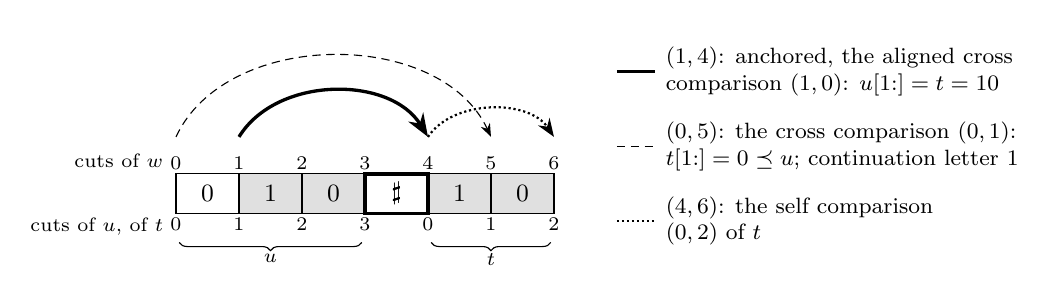
\begin{tikzpicture}[>=Stealth,font=\small,x=0.8cm,y=1cm,
    every node/.style={inner sep=1.5pt},
    cell/.style={draw,minimum width=0.8cm,minimum height=0.5cm,inner sep=0pt},
    lb/.style={font=\scriptsize,inner sep=1pt},
    side/.style={font=\footnotesize,anchor=west,align=left}]
  % the word w = u # t
  \foreach \l/\f [count=\i from 0] in {0/white,1/black!12,0/black!12,\sep/white,1/black!12,0/black!12}
    \node[cell,fill=\f] (c\i) at (\i+0.5,0) {$\l$};
  \node[cell,very thick] at (3.5,0) {$\sep$};
  \foreach \i in {0,...,6}
    \node[lb,anchor=south] at (\i,0.27) {$\i$};
  \node[lb,anchor=east] at (-0.15,0.42) {cuts of $w$};
  \foreach \i in {0,...,3}
    \node[lb,anchor=north] at (\i,-0.27) {$\i$};
  \foreach \e in {0,1,2}
    \node[lb,anchor=north] at (4+\e,-0.27) {$\e$};
  \node[lb,anchor=east] at (-0.15,-0.42) {cuts of $u$, of $t$};
  \draw[decorate,decoration={brace,amplitude=3pt,mirror}] (0.05,-0.62) -- (2.95,-0.62)
    node[midway,below=3pt,lb]{$u$};
  \draw[decorate,decoration={brace,amplitude=3pt,mirror}] (4.05,-0.62) -- (5.95,-0.62)
    node[midway,below=3pt,lb]{$t$};
  % the anchored comparison (1,4)
  \draw[very thick,->] (1,0.72) .. controls (1.6,1.5) and (3.4,1.5) .. (4,0.72);
  % the cross comparison (0,5) and the self comparison (4,6)
  \draw[densely dashed,->] (0,0.72) .. controls (0.8,2.1) and (4.2,2.1) .. (5,0.72);
  \draw[densely dotted,thick,->] (4,0.72) .. controls (4.4,1.2) and (5.6,1.2) .. (6,0.72);
  % legend
  \draw[very thick] (7.0,1.55) -- (7.6,1.55);
  \node[side] at (7.7,1.55) {$(1,4)$: anchored, the aligned cross\\ comparison $(1,0)$: $\wsuf u1=t=10$};
  \draw[densely dashed] (7.0,0.6) -- (7.6,0.6);
  \node[side] at (7.7,0.6) {$(0,5)$: the cross comparison $(0,1)$:\\ $\wsuf t1=0\pre u$; continuation letter $1$};
  \draw[densely dotted,thick] (7.0,-0.35) -- (7.6,-0.35);
  \node[side] at (7.7,-0.35) {$(4,6)$: the self comparison\\ $(0,2)$ of $t$};
\end{tikzpicture}
\caption{The separator word $w=u\sep t$ for $u=010$ and $t=10$, the word of
\cref{ex:mo-loses-tower}; each arrow points from the first cut of a
comparison to its second. The cut $x\le3$ of $w$ is the cut $x$ of $u$, and the
cut $4+e$ is the cut $e$ of $t$. Every comparison of $w$ joins a cut of $u$ to
a cut of $t$, as the cross comparison $(0,5)$ does, or two cuts of $t$, as
$(4,6)$ does (\cref{lem:mo-sep}). The comparison $(1,4)$ is anchored: its
matched factor $\wsub w13=10$ (shaded) ends right before the separator and
equals the suffix $\wsuf w4$. This is how a head event, an equality of two
suffixes, appears in $w$; a cross comparison that is not aligned, such as
$(0,5)$, has a continuation letter inside $u$. The anchored comparisons of $w$
are $(1,4)$, $(2,5)$ and $(3,6)$.}
\Description{The word 0 1 0 separator 1 0 in six cells, the separator cell
framed thickly, with the cuts 0 to 6 of the word written above and, below,
the cuts 0 to 3 of u and 0 to 2 of t, with braces marking u and t. The two
cells 1 0 before the separator and the last two cells 1 0 are shaded. A thick
arrow goes from the cut 1 to the cut 4, a dashed arrow from the cut 0 to the
cut 5, and a dotted arrow from the cut 4 to the cut 6. A legend explains them:
the thick arrow is anchored and is the aligned cross comparison 1, 0; the
dashed arrow is the cross comparison 0, 1 with continuation letter 1; the
dotted arrow is the self comparison 0, 2 of t.}
\label{fig:mo-separator}
\end{figure}


\paragraph{The reader $\RPi$}
Mortality of a safe state is decided by reachability in the safe graph of $A$
(\cref{def:nm-kinds}). The reader $\RPi$ over $\Gamma=\Sigma\sqcup\{\sep\}$
reads $u\sep t$ in three phases.
\begin{itemize}[leftmargin=*]
\item On the spine, its states $\sPre(q,q')$, with $q\in S_A\setminus\Bad$
  and $q'\in S_{A'}$, follow $A$ and $A'$.
\item On the target up to its first rejected cut, its states
  $\sAct(r,r')$, with $r\in S_B$ and $r'\in S_{B'}$, follow $B$ and $B'$.
\item After the first rejected cut, its states $\sDone(r',k)$, with
  $r'\in S_{B'}$ and $1\le k\le N_A$, follow $B'$ and count the letters read,
  capped at $N_A$.
\end{itemize}
A state $\sSink$ absorbs every failure. The automata $A$, $B$, $A'$, $B'$
start in their state $0$ (\cref{def:ex-ss2self}); the start state of $\RPi$ is
$\sPre(0,0)$, or $\sSink$ if $0\in\Bad$. For a letter $i\in\Sigma$ the
transitions are
\[
\begin{aligned}
 \sPre(q,q')&\xrightarrow{i}\sPre(A(q,i),A'(q',i))
   \ \text{if }A(q,i)\notin\Bad,\text{ else }\sSink,\\
 \sPre(q,q')&\xrightarrow{\sep}\sAct(0,0)
   \ \text{if $q$ is mortal},\text{ else }\sSink,\\
 \sAct(r,r')&\xrightarrow{i}\sDone(B'(r',i),1)
   \ \text{if }r\in\Rej,\text{ else }\sAct(B(r,i),B'(r',i)),\\
 \sDone(r',k)&\xrightarrow{i}\sDone(B'(r',i),\min(k+1,N_A)),
\end{aligned}
\]
and every other transition, in particular every transition on $\sep$ after the separator,
leads to $\sSink$. The rejected states are $\sAct(r,r')$ with $r\in\Rej$ and
$\sDone(r',k)$ with $k\le N_A-1$. The admission relation consists of the pairs
\[
 \bigl(\sPre(q,q'),\sAct(r,r')\bigr)\ \text{with }(q,r)\in\Guard,
 \qquad
 \bigl(\sAct(r_1,r'_1),\sAct(r_2,r'_2)\bigr)\ \text{with }(r_1,r_2)\in\GuardS,
\]
and no others. The relation $\Pi$ relates $\sPre(q,q')$ to $\sAct(r,r')$ and to
$\sDone(r',k)$ iff $(q',r')\in\Head$, and relates no other pairs.

Thus $\RPi$ reads the separator only from a mortal state, rejects a word only if
fewer than $N_A$ letters follow the first rejected cut of the target, and lets
$\Pi$ compare the head automata on the two sides of the separator. The target
automaton is kept up to and including the first rejected cut, because events
and self events may end there; after it, events and self events no longer
exist (\cref{def:ex-events}), so only $B'$ and the counter remain. The admissions
from the self guard $\GuardS$ are the only difference from a reader for
instances without self events; the compression below allows an arbitrary admission relation.

For a reader, only the states reachable from its start state matter: the
restriction to them is again a reader, with the same run on every word and
hence the same holes and $\Pi$-holes. Let $r_I$ and $z_I$ be the numbers of
states of the product automata $A\times A'$ and $B\times B'$ reachable from
their start states, so that $r_I\le N_AN_{A'}$ and $z_I\le N_BN_{B'}$, and put
\[
 \Nbar=1+r_I+z_I+N_AN_{B'},\qquad d_I=2\Nbar N_A-1 .
\]

\begin{lemma}[The $\Pi$-reader]\label{lem:mo-pi-reader}
The reader $\RPi$ and the relation $\Pi$ are computable from $I$, and:
\begin{enumerate}[label=(\roman*),leftmargin=*]
\item at most $\Nbar$ states of $\RPi$ are reachable from its start state;
\item a word $w$ over $\Sigma\sqcup\{\sep\}$ is a $\Pi$-hole of $\RPi$ iff
  $w=u\sep t$ with $u,t\in\Sigma^*$ and $(u,t)$ a mortal hole of $I$;
\item for such $w$ the first rejected cut is $\len u+1+J(t)$, so the rejected
  tail of $w$ is $\len t-J(t)$.
\end{enumerate}
\end{lemma}

On $u\sep t$, the state at a cut $x\le\len u$ carries $A_x(u)$ and $A'_x(u)$
while $u$ is safe, and the state at the cut $\len u+1+e$ carries $B_e(t)$ up to
$J(t)$ and $B'_e(t)$ throughout. By \cref{lem:mo-sep}, the admitted comparisons
are then exactly the events and the self events, and $\Pi$ on the anchored
comparisons is exactly the head condition. The proof is in
\cref{app:mo-separator}.

\subsection{The Depth of the Separator Word}\label{sec:mo-depth}

The length bound of the bounded-depth search grows with the depth of the word
(\cref{thm:bg-search}). For a mortal hole, the depth of the separator word is
bounded at once.

\begin{lemma}[Depth of mortal holes]\label{lem:mo-depth}
Every mortal hole $(u,t)$ of $I$ satisfies $\depth(u\sep t)\le d_I$.
\end{lemma}

\begin{proof}
By \cref{lem:mo-pi-reader}, $u\sep t$ is a nonempty rejected word of the
reachable part of $\RPi$, a reader with at most $\Nbar$ states, and its rejected
tail is $\len t-J(t)\le N_A-1$. \Cref{thm:bg-depth} gives
$\depth(u\sep t)\le2\Nbar((N_A-1)+1)-1=d_I$.
\end{proof}

The bound is coarse, since it involves the spine and head automata through
$\Nbar$, but it enters the final estimate only through a polynomial in $\Nbar$
and $N_A$, and changes only the constant in the exponent
(\cref{lem:mo-estimate}).

\subsection{Positive Channels}\label{sec:mo-channels}

The bounded-depth search sees each level of the hierarchy through a lettered
monitor, the derivative of the monitor one level below
(\cref{def:bg-monitor,def:bg-derivative}); the derivatives carry the negative
conditions, because a comparison of one level reappears at the next as a
comparison of blocks or as a test in the final target. We carry the positive
condition in the same way. At level $0$ it is an anchored comparison in $\Pi$,
a comparison together with a test of its continuation letter; one level up, the
continuation letter is the first letter of the expansion of a block, or a
letter inside the last block, and the comparison may have become a test of the
final label. Five components cover all the forms that arise.

\begin{definition}[Positive channel]\label{def:mo-channel}
Let $\mathcal M$ be a lettered monitor over an alphabet $\Gamma$ with state set
$\mathcal Q$. A \emph{positive channel} $\Theta=(F,R,S,S',\Phi)$ on $\mathcal M$
consists of a predicate $F\subseteq\mathcal Q\times\Gamma$, three relations
$R$, $S$ and $S'$ on labels, and a set $\Phi\subseteq\Gamma$ of letters. For a
nonempty word $v$ with labels $L_0,\ldots,L_{\len v}$, the \emph{positive
condition} $\PosOp_\Theta(v)$ holds iff one of the following clauses holds:
\begin{description}[leftmargin=2.8em,font=\normalfont]
\item[(F)] $F(L_{\len v})$;
\item[(R)] some comparison $(x,y)$ of $v$ with $y<\len v$ has $R(L_x,L_y)$ and
  $v[x+\len v-y]\in\Phi$;
\item[(S)] some cut $x<\len v$ has $S(L_x,L_{\len v})$;
\item[(S$'$)] some cut $x<\len v$ has $S'(L_x,L_{\len v})$ and $v[x]\in\Phi$.
\end{description}
A \emph{positive hole} of $(\mathcal M,\Theta)$ is a hole $v$ of $\mathcal M$
with $\PosOp_\Theta(v)$.
\end{definition}

Clauses (R) and (S$'$) together say that some comparison has its labels in a
relation, $R$ if it is not terminal and $S'$ if it is, and its continuation
letter in $\Phi$; the continuation letter of the terminal comparison $(x,\len
v)$ is $v[x]$. Clauses (F) and (S) are tests without a continuation letter.
They are empty at level $0$, but derivatives move witnesses into them, as the
derivatives of lettered monitors move admissions into the terminal relation and the
final target.

For a reader $(\mathcal M,\Adm,\Rej)$ over $\Gamma\ni\sep$ with start $q_0$ and
$\Pi\subseteq Q\times Q$, the \emph{base channel} on the lettered monitor of
the reader (\cref{def:bg-monitor}) is
\[
 \Theta_\Pi=(\varnothing,\widehat\Pi,\varnothing,\widehat\Pi,\{\sep\}),
 \qquad
 \widehat\Pi(L,L')\iff(\den L,\den L')\in\Pi .
\]

\begin{lemma}[The base channel]\label{lem:mo-base}
A nonempty word $w$ satisfies $\PosOp_{\Theta_\Pi}(w)$ iff it has an anchored
comparison $(x,y)$ with $(q_x,q_y)\in\Pi$. Hence the $\Pi$-holes of the reader
are exactly the positive holes of its lettered monitor with the base channel.
\end{lemma}

\begin{proof}
Since $\den L_i=q_i$, clause (R) is an anchored comparison $(x,y)$ with
$y<\len w$ and $(q_x,q_y)\in\Pi$, and clause (S$'$) is the same for a terminal
comparison $(x,\len w)$, whose continuation letter is $w[x]$; clauses (F) and
(S) are empty. The reader and its lettered monitor have the same nonempty
holes.
\end{proof}

The derivative of a channel uses the shifted blocks of
\cref{def:bg-derivative}. The letter that follows the position $g$ of the
shifted block of $X$ is $(X\ell)[g]$: the letter $X[g]$ for $g<\len X$, and
the marker that opens the next shifted block for $g=\len X$.

\begin{definition}[Derivative of a channel]\label{def:mo-channel-derivative}
Let $\Theta=(F,R,S,S',\Phi)$ be a positive channel on $\mathcal M$ and
$\ell\in\Gamma$. The \emph{derivative} $\Theta_\ell=(F_\ell,R_\ell,S_\ell,
S'_\ell,\Phi_\ell)$ is the positive channel on $\mathcal M_\ell$ given by
\[
\begin{aligned}
 \Phi_\ell&=\{X:(X\ell)[0]\in\Phi\},\\
 R_\ell((\zeta,X),(\zeta',X'))&\iff X=xy,\ X'=x'y,\
   R\bigl(\lab_{\len x}(\zeta,X),\lab_{\len{x'}}(\zeta',X')\bigr)
   \text{ for some }x,x',y,\\
 S'_\ell&=R_\ell,\\
 S_\ell((\zeta,X),(\zeta',X'))&\iff\ptest(\zeta,X;\delta_\ell(\zeta',X')),\\
 F_\ell(\zeta,X)&\iff F(\delta_\ell(\zeta,X),\ell)\ \text{or}\
   \ptest(\zeta,X;\delta_\ell(\zeta,X)),
\end{aligned}
\]
where the \emph{positive terminal test} is
\[
\begin{aligned}
 \ptest(\zeta,X;\zeta'')\iff{}&\text{for some }g\le\len X:\
 S\bigl(\lab_g(\zeta,X),(\zeta'',\ell)\bigr),\\
 &\text{or }S'\bigl(\lab_g(\zeta,X),(\zeta'',\ell)\bigr)\text{ and }
 (X\ell)[g]\in\Phi,
\end{aligned}
\]
and every relation with the start label $\triangleright$ of $\mathcal M_\ell$ as
an argument is false.
\end{definition}

The relation $R_\ell$ is built from $R$ exactly as the derived admission
$\Lambda_\ell$ is built from $\Lambda$, and the positive terminal test is the
analog of the terminal test in $\Lfin_\ell$ and $\Tfin_\ell$: it relates a
position of a block, possibly the closing marker, to the final label, which is
$(\zeta'',\ell)$ when the final marker is read from the state $\zeta''$. The predicate $F$ concerns
only the final label, so it enters $F_\ell$ but not $S_\ell$. The set
$\Phi_\ell$ tests the first letter of the expansion of a block, because the
continuation letter of a comparison of the expansion is the first letter of the
expansion of the continuation letter of the corresponding comparison of blocks
(\cref{lem:mo-transport}). This is how the anchoring equation travels up the
hierarchy: ``followed by $\sep$'' at level $0$ becomes ``followed by a block
whose expansion starts with $\sep$'' at level $1$, and so on.

\begin{lemma}[Positive desubstitution]\label{lem:mo-desub}
Let $\Theta$ be a positive channel on $\mathcal M$, let $\ell\in\Gamma$, and let
$v$ be the expansion of a nonempty word $v'$ of blocks avoiding $\ell$. Then
$\PosOp_\Theta(v)\iff\PosOp_{\Theta_\ell}(v')$. Consequently $v$ is a positive
hole of $(\mathcal M,\Theta)$ iff $v'$ is a positive hole of
$(\mathcal M_\ell,\Theta_\ell)$.
\end{lemma}

The second claim follows from the first and \cref{lem:bg-desub}. The proof of
the first, in \cref{app:mo-desub}, translates each clause by the label facts
\cref{eq:bg-label-facts} and the alignment lemma (\cref{lem:bg-alignment}): a
nonterminal comparison of $v$ becomes a comparison of blocks, read by $R_\ell$
or, if it ends at the last cut, by $S'_\ell$; a terminal comparison of $v$ that
starts in the block $X_i$ becomes a test of $S_\ell$ or, if $X_i$ is the last
block, of $F_\ell$.

\begin{corollary}[Channel towers]\label{cor:mo-tower}
Let $\mathcal M_0$ be a lettered monitor with $N$ states, $\Theta_0$ a positive
channel on it, and $w$ a nonempty word with canonical hierarchy
$(w_j,\ell_j)$. Put $\mathcal M_{j+1}=(\mathcal M_j)_{\ell_j}$ and
$\Theta_{j+1}=(\Theta_j)_{\ell_j}$. Then $w$ is a positive hole of
$(\mathcal M_0,\Theta_0)$ iff $w_j$ is a positive hole of
$(\mathcal M_j,\Theta_j)$, for every $j$.
\end{corollary}

\begin{proof}
Each $w_{j+1}$ is a nonempty word of blocks avoiding $\ell_j$, with expansion
$w_j$. Apply \cref{lem:mo-desub} at each level.
\end{proof}

Neither the lemma nor the corollary assumes that $\sep$ occurs once, or at
all, and the reader may have an arbitrary admission relation.

\begin{example}[A witness travels up the tower]\label{ex:mo-loses-tower}
Take $\Gamma=\{0,1,\sep\}$, the five states $0,\ldots,4$ with start $0$, the
transitions
\begin{center}
\begin{tabular}{@{}c|ccccc@{}}
state & $0$ & $1$ & $2$ & $3$ & $4$\\
\hline
on $0$ & $3$ & $0$ & $0$ & $3$ & $0$\\
on $1$ & $1$ & $1$ & $4$ & $0$ & $2$\\
on $\sep$ & $4$ & $3$ & $2$ & $4$ & $0$
\end{tabular}
\end{center}
$\Adm=\varnothing$, $\Rej=\{0,1\}$ and $\Pi=\{(3,4),(4,2)\}$. The word
$w=010\sep10$ has the run $0,3,0,3,4,2,0$ and ends in a rejected state, so it is
a hole. Its anchored comparisons are $(1,4)$, $(2,5)$ and $(3,6)$, with state
pairs $(3,4)$, $(0,2)$ and $(3,0)$. Only the first, which matches the factor
$10$ before the separator with the final $10$, is in $\Pi$, so $w$ is a
$\Pi$-hole; for the base channel, its witness $(1,4)$ is clause (R). The
hierarchy of $w$ is $w_1=abc$ with $a=[\eps]$, $b=[1]$ and $c=[\sep1]$, and
$w_2=[ab]$, a single letter. At level $1$, with the marker $0$, the cut $1$
lies in the block $X_1=1$ and the cut $4$ in the last block $X_2=\sep1$, both
with the common suffix $1$; so the comparison of blocks is the terminal pair
$(2,3)$ of $w_1$, and the witness becomes clause (S$'$) at the cut $2$, with
continuation letter $c$, which lies in $\Phi_1$ because its expansion starts
with $\sep$. At level $2$, with the marker $c$, the cut $2$ of $w_1$ is the end
of the only block $ab$ of $w_2$; so the witness becomes the second disjunct of
the final target $F_2$, through the positive terminal test at the position
$\len{ab}$, whose letter is the marker $c\in\Phi_1$. Clause (R) at level $0$
has become clause (S$'$) at level $1$ and clause (F) at level $2$.
\end{example}

\Cref{fig:mo-tower} draws the three levels of this example. Each level sees
the witness only through its own letters: once the matched factor $10$ has
become the single letter $b$ and the separator the first letter of $c$, the
comparison turns into a test at the boundary between $b$ and $c$, and one
level higher into a test of the final label.

\begin{figure}[tbp]
\centering
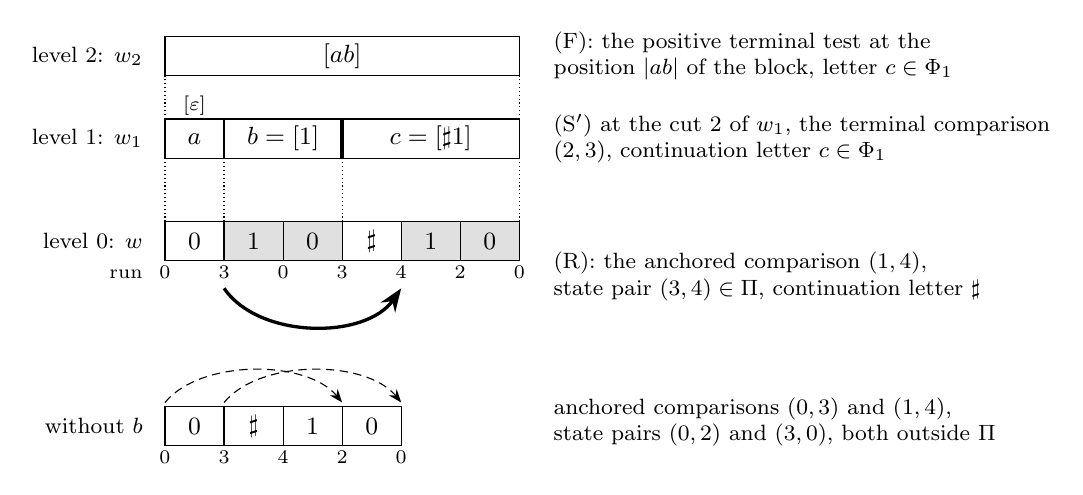
\begin{tikzpicture}[>=Stealth,font=\small,x=0.75cm,y=1cm,
    every node/.style={inner sep=1.5pt},
    cell/.style={draw,minimum height=0.5cm,inner sep=0pt},
    lb/.style={font=\scriptsize,inner sep=1pt},
    side/.style={font=\footnotesize,anchor=west,align=left},
    lvl/.style={font=\footnotesize,anchor=east}]
  % level 0: w = 010#10 with its run
  \foreach \l/\f [count=\i from 0] in {0/white,1/black!12,0/black!12,\sep/white,1/black!12,0/black!12}
    \draw[fill=\f] (\i,-0.25) rectangle node{$\l$} (\i+1,0.25);
  \foreach \q [count=\i from 0] in {0,3,0,3,4,2,0}
    \node[lb,anchor=north] at (\i,-0.28) {$\q$};
  \draw[very thick,->] (1,-0.6) .. controls (1.6,-1.25) and (3.4,-1.25) .. (4,-0.6);
  \node[lvl] at (-0.3,0) {level $0$: $w$};
  \node[lvl,font=\scriptsize] at (-0.3,-0.42) {run};
  \node[side] at (6.5,-0.45) {(R): the anchored comparison $(1,4)$,\\
    state pair $(3,4)\in\Pi$, continuation letter $\sep$};
  % level 1: w_1 = abc, marker 0
  \draw (0,1.05) rectangle node{$a$} (1,1.55);
  \draw (1,1.05) rectangle node{$b=[1]$} (3,1.55);
  \draw (3,1.05) rectangle node{$c=[\sep1]$} (6,1.55);
  \node[lb,anchor=south] at (0.5,1.55) {$[\eps]$};
  \foreach \x in {0,1,3,6} \draw[densely dotted] (\x,0.25) -- (\x,1.05);
  \draw[very thick] (3,1.05) -- (3,1.55);
  \node[lvl] at (-0.3,1.3) {level $1$: $w_1$};
  \node[side] at (6.5,1.3) {(S$'$) at the cut $2$ of $w_1$, the terminal comparison\\
    $(2,3)$, continuation letter $c\in\Phi_1$};
  % level 2: w_2 = [ab], marker c
  \draw (0,2.1) rectangle node{$[ab]$} (6,2.6);
  \foreach \x in {0,6} \draw[densely dotted] (\x,1.55) -- (\x,2.1);
  \node[lvl] at (-0.3,2.35) {level $2$: $w_2$};
  \node[side] at (6.5,2.35) {(F): the positive terminal test at the\\
    position $\len{ab}$ of the block, letter $c\in\Phi_1$};
  % after deleting the column of b
  \begin{scope}[yshift=-2.35cm]
    \foreach \l/\f [count=\i from 0] in {0/white,\sep/white,1/white,0/white}
      \draw[fill=\f] (\i,-0.25) rectangle node{$\l$} (\i+1,0.25);
    \foreach \q [count=\i from 0] in {0,3,4,2,0}
      \node[lb,anchor=north] at (\i,-0.28) {$\q$};
    \draw[densely dashed,->] (0,0.3) .. controls (0.6,0.85) and (2.4,0.85) .. (3,0.3);
    \draw[densely dashed,->] (1,0.3) .. controls (1.6,0.85) and (3.4,0.85) .. (4,0.3);
    \node[lvl] at (-0.3,0) {without $b$};
    \node[side] at (6.5,0.05) {anchored comparisons $(0,3)$ and $(1,4)$,\\
      state pairs $(0,2)$ and $(3,0)$, both outside $\Pi$};
  \end{scope}
\end{tikzpicture}
\caption{A positive witness travels up the hierarchy
(\cref{ex:mo-loses-tower,ex:mo-loses}). Bottom up: the hole $w=010\sep10$ of
the reader of \cref{ex:mo-loses-tower} with its run, the word $w_1=abc$ of
blocks for the marker $0$, each letter drawn over its block and the marker that
closes it, and the one-letter word $w_2=[ab]$ for the marker $c$. The anchored
witness $(1,4)$ in $\Pi$, whose matched factor $10$ is shaded, is clause (R) of
the base channel at level $0$, clause (S$'$) of the derived channel at level
$1$, and clause (F) at level $2$, where it is a test of the final label
(\cref{def:mo-channel,lem:mo-desub}). The compression for plain entailment sees
no difference between the prefixes $a$ and $ab$ of the block and deletes the
column of $b$, which carries the matched factor $10$; the result $0\sep10$
(last row) is still a hole, but no longer a $\Pi$-hole. Recording the channel in
the summaries keeps $b$.}
\Description{Three stacked rows of cells. The bottom row is the word 0 1 0
separator 1 0, with the states 0 3 0 3 4 2 0 of its run under the cuts and a
thick arrow below from the cut 1 to the cut 4; the cells 1 0 before the
separator and the last cells 1 0 are shaded. The middle row has the letters a
over the first cell, b equal to the block 1 over the next two cells, and c
equal to the block separator 1 over the last three cells; the boundary between
b and c, the cut 2, is drawn thick. The top row is one cell, the block a b,
over the whole word. Notes to the right name the clause of the witness at each
level: R at level 0, S prime at level 1, F at level 2. A separate row at the
bottom shows the word 0 separator 1 0 with the run 0 3 4 2 0 and two dashed
arrows, from the cut 0 to the cut 3 and from the cut 1 to the cut 4, whose
state pairs are outside Pi.}
\label{fig:mo-tower}
\end{figure}


\subsection{Anchored Compression}\label{sec:mo-compression}

\paragraph{What the compression for plain entailment misses}
Steps~2 and~4 of the bounded-depth search (\cref{sec:bg-hierarchy}, and
precisely \cref{app:bg-search}) replace the word by another one: step~2 merges
isolated letters with the same exchange type, and step~4 deletes the columns
between two cuts of a column word with equal summaries. Each of them only has
to keep the word a hole. A $\Pi$-hole must also \emph{contain} an anchored
comparison in $\Pi$. The exchange types and summaries record nothing about
$\Pi$, so a column deletion, and similarly a merge, can destroy every such
comparison.

\begin{example}[The compression for plain entailment loses the anchored witness]\label{ex:mo-loses}
Continue \cref{ex:mo-loses-tower}. Step~4 shortens the block $ab$ over the
level-$1$ monitor with the marker $c$. In this monitor $c$ leads every state to
$2$, and the exits of the shifted blocks of the prefixes $a$ and $ab$ are $0$
from every entry state; since $\Adm$ is empty, all terminal and admission bits
are false. So the summaries after $a$ and after $ab$ coincide, and step~4
deletes the column holding $b$. Expanding $[a]$ gives $0\sep10$
(\cref{fig:mo-tower}, last row), with run
$0,3,4,2,0$: a hole, whose anchored comparisons $(0,3)$ and $(1,4)$ have the
state pairs $(0,2)$ and $(3,0)$, both outside $\Pi$. The deleted letter $b$ is
exactly the letter whose expansion is the matched factor $10$ before the
separator.
\end{example}

The bound of the next theorem is an explicit function $\Lensharp(N,d)$. Like
$\holeBound(N,d)$ of \citet{Zhao26}, it is built from constants $\sCsharp$,
$\sAsharp$, $\sGsharp$ and $\scolsharp$, which bound the anchored exchange
types, the protected and isolated letters, the dictionaries and the positive
column summaries. They are defined in \cref{eq:mo-constants}, increase in each
argument, and do not depend on the alphabet; the theorem states their closed
form.

\begin{theorem}[Anchored compression]\label{thm:mo-anchored}
Let $(\mathcal M,\Adm,\Rej)$ be a reader with $N\ge1$ states over a finite
alphabet $\Gamma\ni\sep$, let $\Pi\subseteq Q\times Q$, and let $d\ge0$. If the
reader has a $\Pi$-hole of depth at most $d$, then it has a $\Pi$-hole of depth
at most $d$ and length at most $\Lensharp(N,d)$. More generally, for every
lettered monitor $\mathcal M_0$ with $N$ states over any alphabet and every
positive channel $\Theta_0$ on it, if $(\mathcal M_0,\Theta_0)$ has a positive
hole of depth at most $d$, then it has one of depth at most $d$ and length at
most $\Lensharp(N,d)$. Moreover, with
$\Xisharp(N,d)=6N^2+10N(N+d)(d+1)+7N+3d+4$,
\[
 \sGsharp(N,d)\le2^{\Xisharp(N,d)}
 \qquad\text{and}\qquad
 \Lensharp(N,d)\le2^{2^{5\Xisharp(N,d)}} .
\]
\end{theorem}

The theorem is the analog of \cref{thm:bg-search} for $\Pi$-holes. It
preserves the \emph{existence} of an anchored comparison in $\Pi$, not its
coordinates or its state pair; to keep a particular state pair, apply it to
the singleton relation of that pair. It needs no uniqueness of the separator.
The first claim is the second one for the lettered monitor of the reader and
the base channel, by \cref{lem:mo-base}.

\paragraph{Why recording the channel suffices}
The positive condition is a property of the labels at the cuts of a witness
and of one letter, the continuation letter. The shortenings of \citet{Zhao26}
(steps~2--4 in \cref{sec:bg-hierarchy}) preserve such data once they record
the channel. The merges preserve the state run, the comparison positions, and
the relevant channel tests; the top shortening preserves the labels of the
cuts of the witness, which it never deletes, and the letter, which is constant
on a unary word; and the
summaries determine the derived channel, so that agreement preserves labels
and letters up to renaming. This is why recording the channel suffices, with
no further condition on the separator.

\begin{proof}[Proof outline]
The complete proof is in \cref{app:mo-proof}. The proof of \cref{thm:bg-search} merges letters
with equal exchange types and deletes columns between equal summaries. We add
the five components of the channel to both, so that each shortening keeps some
anchored witness, though not necessarily the original one; every argument
about the negative conditions is reused unchanged. Let $w$ be a positive hole
of depth $D\le d$, with hierarchy $(w_j,\ell_j)$; we follow the five steps of
that proof (\cref{sec:bg-hierarchy}).
\begin{enumerate}[leftmargin=*]
\item \emph{Towers.} By \cref{cor:mo-tower}, $w_j$ is a positive hole of
  $(\mathcal M_j,\Theta_j)$ for every $j$; the clause of the witness may change
  from level to level (\cref{ex:mo-loses-tower}).
\item \emph{Merging letters.} In the terms of step~2 in \cref{sec:bg-hierarchy},
  a letter of $w_i$ is unprotected if it is neither the marker nor a letter of
  the start prefix, and isolated if, moreover, all its unequal comparison
  partners are protected; its exchange type is the table of how $\mathcal M_i$
  treats it when it is read from an ordinary state. The
  \emph{anchored exchange type} of an unprotected letter $a$ at a level
  $1\le i<D$ adds the same table for the channel: the row of $F_i$ at $a$, the
  self table, the protected rows and the initial row of each of $R_i$, $S_i$
  and $S'_i$, and the bit $[a\in\Phi_i]$ (\cref{def:mo-type}). There are at
  most $\sCsharp(N,d)$ anchored types (\cref{lem:mo-types}). Merging two
  isolated letters with the same anchored type keeps the comparisons and the
  run of the level, so it keeps every value of $\Lambda_i$, $\Lfin_i$, $R_i$,
  $S_i$ and $S'_i$ at the comparisons of the level, exactly as in the
  argument of \citet{Zhao26} for $\Lambda_i$ and $\Lfin_i$; it keeps the final label,
  because the marker is protected; and it keeps the position of every
  continuation letter and changes that letter at most from $a$ to $b$, which
  have the same bit. So the merged level is again positive, and expanding it
  gives a positive hole of $(\mathcal M_0,\Theta_0)$ of the same depth, no
  longer, with a smaller dictionary (\cref{lem:mo-exchange}). Repeated merges
  bound the dictionary, the set of letters, of every level $i\ge1$ by
  $\sGsharp(N,d)$ (\cref{lem:mo-dictionary}). A merge is not injective and
  gives no agreement; after each merge the hierarchy and the towers are
  recomputed.
\item \emph{The top level.} The top level $w_D$ is unary. Deleting a loop
  between two cuts with equal states keeps a hole (\cref{lem:bg-unary}), and it
  keeps the positive witness if no cut of the witness is deleted. Protecting the
  at most three cuts of one witness leaves at most three stretches of
  pairwise distinct states, so $\len{w_D}\le3(N+D)$ after shortening
  (\cref{lem:mo-unary}).
\item \emph{Deleting columns.} The \emph{positive summary} of a tuple of blocks
  extends the summary of \cref{app:bg-search} by fields that record the positive terminal
  test, the last pending $S'$-test (a test at the end of a block, whose letter
  is the next one to be read), whether a block is empty, the bit $\Phi$ of its
  first letter, and the lift $R_\ell$ between pairs of blocks. These fields are
  updated column by column and determine the derived channel on the blocks, in
  particular $S_\ell$ without an $F$-term and $F_\ell$ with one
  (\cref{lem:mo-summary}). Deleting the columns between two cuts with equal
  positive summaries therefore keeps both the derived monitor and the derived
  channel (\cref{lem:mo-columns}). In \cref{ex:mo-loses}, the pending
  $S'$-test is false after $a$ and true after $ab$, where it records the
  witness $(1,4)$; so the positive summaries after $a$ and after $ab$ differ,
  and the column holding $b$ is kept (\cref{ex:mo-loses-fields}).
\item \emph{Agreement and the bound.} Agreement of monitors on the letters in
  use (step~4 in \cref{sec:bg-hierarchy}) is extended to the five components
  of the channel, which must also take equal values at corresponding letters
  and labels. Extended agreement preserves positive holes and is preserved
  under derivation (\cref{lem:mo-agreement}). The supported compression of
  \citet{Zhao26}, which shortens the letters in use level by level from the top,
  then runs unchanged with the positive summaries (\cref{lem:mo-compression}).
  Each of the at most $d$ expansions costs a factor
  $\scolsharp(N+d+1,\sGsharp(N,d))$, and the top level costs $3(N+d+1)$, which
  gives $\Lensharp(N,d)$. The new top word is a positive hole of the new top
  monitor, and \cref{lem:bg-desub,lem:mo-desub} reconstruct a positive hole of
  $(\mathcal M_0,\Theta_0)$ of depth at most $D$.
\end{enumerate}
The closed-form estimate is \cref{lem:mo-closed-form}.
\end{proof}

\subsection{Short Mortal Holes and Decidability}\label{sec:mo-short}

Put
\[
 \Lensharp_I=\Lensharp(\Nbar,d_I),
\]
with $\Nbar$ and $d_I$ as in \cref{sec:mo-separator}, and recall the bound
$\Lnm$ of \cref{thm:nm-three-cases}, evaluated at the state counts
$(N_A,N_B,N_{A'},N_{B'})$.

\begin{theorem}[Short mortal holes]\label{thm:mo-short}
If $I$ has a mortal hole, then it has a mortal hole $(u,t)$ with
$\len u+1+\len t\le\Lensharp_I$. No assumption on $I$ is needed; in particular
(FH) is not used.
\end{theorem}

\begin{proof}
Let $(u,t)$ be a mortal hole. By \cref{lem:mo-pi-reader}, $w=u\sep t$ is a
$\Pi$-hole of $\RPi$, and of its reachable part, a reader with at most $\Nbar$
states over the finite alphabet $\Sigma\sqcup\{\sep\}$. By \cref{lem:mo-depth},
$\depth(w)\le d_I$. By \cref{thm:mo-anchored} and monotonicity of $\Lensharp$,
the reachable part has a $\Pi$-hole $\tilde w$ of length at most
$\Lensharp_I$. By \cref{lem:mo-pi-reader}(ii), $\tilde w=\tilde u\sep\tilde t$
with $(\tilde u,\tilde t)$ a mortal hole, and
$\len{\tilde u}+1+\len{\tilde t}=\len{\tilde w}$.
\end{proof}

\begin{corollary}[Mortal holes are decidable]\label{cor:mo-decidable}
It is decidable whether an instance of the two-word hole problem with self
events has a mortal hole.
\end{corollary}

\begin{theorem}[Short holes]\label{thm:mo-decide}
Let $I$ satisfy (FH). Then $I$ has a hole iff it has a hole $(u,t)$ with
\[
 \len u+\len t<\max\bigl(\Lnm(N_A,N_B,N_{A'},N_{B'}),\ \Lensharp_I\bigr).
\]
In particular, it is decidable whether an instance with forced target heads
has a hole.
\end{theorem}

\begin{proof}
By \cref{cor:nm-short-holes}, $I$ has a hole iff it has a hole with
$\len u+\len t<\Lnm(N_A,N_B,N_{A'},N_{B'})$ or a mortal hole. In the second case
\cref{thm:mo-short} gives a mortal hole, which is a hole, with
$\len u+\len t<\Lensharp_I$. The bound is computable from $I$, and the alphabet
$\Sigma$ is finite, so there are finitely many candidate pairs; for each, the
conditions of \cref{def:ex-ss2self} are checked over finitely many cuts.
\end{proof}

The proof of \cref{cor:mo-decidable} is the same enumeration with the bound of
\cref{thm:mo-short} and the additional tests that $A(u)$ is mortal and
$\len t-J(t)<N_A$ (\cref{app:mo-estimates}). Both bounds are independent of the
alphabet, and hence of the arity; the alphabet enters only the number of
candidate pairs. For $n=0$ the only candidate is $(\eps,\eps)$.

\paragraph{The size of the bound}
Write $E_1(x)=2^x$ and $E_{k+1}(x)=2^{E_k(x)}$.

\begin{lemma}[Mortal bound]\label{lem:mo-estimate}
Let $\alpha\ge3$ and $\beta\ge0$ be integers with $\Nbar\le2^\alpha$ and
$N_A\le2^\beta$. Then $\Lensharp_I\le E_3(3\alpha+2\beta+9)$.
\end{lemma}

\begin{corollary}[Mortal bound for extracted instances]\label{cor:mo-extracted}
Let $\varphi$ be a flat system over $X$ and $\psi$ a flat system over $X\cup Z$,
with $v=\len X$, $h=\len Z$ and $s=v+h$. Every extracted instance $I_{pq}$
(\cref{def:ex-instance}) satisfies
\[
 \Lensharp_{I_{pq}}\le E_3(10v+6s+18)\le E_3(16s+18),
\]
for every arity $n$ and every variance. So if $I_{pq}$ has a mortal hole, it
has one whose separator word has length at most $E_3(16s+18)$.
\end{corollary}

\begin{proof}
By \cref{sec:ex-instances}, $N_A=2^{2v}$, $N_B=2^{4v+2h+1}=2^{2v+2s+1}$ and
$N_{A'}=N_{B'}=2^{2s}$, and the reachable pairs of states of $B$ and $B'$ number
at most $N_B$. Hence $r_I\le N_AN_{A'}=2^{2v+2s}$, $z_I\le2^{2v+2s+1}$ and
$N_AN_{B'}=2^{2v+2s}$, so $\Nbar\le1+2^{2v+2s+2}\le2^{2v+2s+3}$.
\Cref{lem:mo-estimate} with $\alpha=2v+2s+3$ and $\beta=2v$ gives
$E_3(3(2v+2s+3)+4v+9)=E_3(10v+6s+18)$, and $v\le s$. The second claim is
\cref{thm:mo-short}. None of these sizes depends on $n$.
\end{proof}

\begin{remark}[Where (FH) is used]\label{rem:mo-fh}
Condition (FH) is used only in \cref{thm:mo-decide}, through
\cref{thm:nm-three-cases}. Every other result of this section, in particular
\cref{thm:mo-short,cor:mo-decidable}, holds for every instance.
\end{remark}

%% assembly -- the main theorem, stated once; counterexample words; the
%% decision procedure as a numbered algorithm with its dependency table;
%% countermodels from counterexample words; counterexample bounds per case;
%% the proof of the main theorem by assembling the earlier sections; and plain
%% entailment as a corollary. The remark on complexity is in complexity.tex.

\providecommand{\parity}{\operatorname{par}}
\providecommand{\Mod}{\operatorname{Mod}}
\providecommand{\CondI}{\textup{(I0)}}
\providecommand{\CondU}{\textup{(U)}}
\providecommand{\CondII}{\textup{(II)}}
\providecommand{\DeadT}{\mathsf{DeadT}}
\providecommand{\DeadU}{\mathsf{DeadU}}
\providecommand{\Fup}[1]{\Fact^{\uparrow}_{#1}}
\providecommand{\Bsrc}{\mathcal B}
\providecommand{\RU}{\mathcal R_{\mathrm U}}
\providecommand{\Lnm}{\mathsf L_{\mathrm{nm}}}
\providecommand{\Eall}{E_{\mathrm{all}}}
\providecommand{\Ereg}{E_{\mathrm{reg}}}
\providecommand{\Efin}{E_{\mathrm{fin}}}
\crefformat{asstep}{Step~#2#1#3}
\Crefformat{asstep}{Step~#2#1#3}
\crefrangeformat{asstep}{Steps~#3#1#4 to~#5#2#6}
\Crefrangeformat{asstep}{Steps~#3#1#4 to~#5#2#6}
\crefmultiformat{asstep}{Steps~#2#1#3}{ and~#2#1#3}{, #2#1#3}{, and~#2#1#3}
\Crefmultiformat{asstep}{Steps~#2#1#3}{ and~#2#1#3}{, #2#1#3}{, and~#2#1#3}
\crefrangemultiformat{asstep}{Steps~#3#1#4 to~#5#2#6}{ and~#3#1#4 to~#5#2#6}{, #3#1#4 to~#5#2#6}{, and~#3#1#4 to~#5#2#6}
\Crefrangemultiformat{asstep}{Steps~#3#1#4 to~#5#2#6}{ and~#3#1#4 to~#5#2#6}{, #3#1#4 to~#5#2#6}{, and~#3#1#4 to~#5#2#6}

\section{The Main Theorem}\label{sec:as}

This section states the main theorem and proves it by assembling the results
of \cref{sec:bg,sec:lf,sec:ch,sec:tc,sec:sm,sec:un,sec:ex,sec:nm,sec:mo}.
Apart from bookkeeping, only two things are proved here: how a
counterexample word yields a countermodel (\cref{lem:as-countermodel}), and
two short estimates that turn the length bounds of the earlier sections into
closed forms (\cref{prop:as-bounds}).

Throughout, the arity $n\ge0$ and the variance $c$ are fixed. For a flat
system $\varphi$ over $X$ and a flat system $\psi$ over $X\cup Z$ we write
\[
 v=\len X,\qquad h=\len Z,\qquad s=v+h,
\]
so that $s$ is the size parameter of \cref{sec:bg-constraints}, counted after
flattening. As in \cref{sec:mo-short}, $E_1(x)=2^x$ and
$E_{k+1}(x)=2^{E_k(x)}$.

\subsection{Statement}\label{sec:as-statement}

When the entailment fails although both systems are satisfiable, the failure
is certified by a single word, which comes from one of the three conditions
of \cref{thm:ch-characterization}.

\begin{definition}[Counterexample words]\label{def:as-certificate}
Let $\varphi$ over $X$ and $\psi$ over $X\cup Z$ be flat systems over $\BFT$,
both satisfiable. A \emph{counterexample word} of $(\varphi,\psi)$ is a word of
one of the following three kinds, together with the signed variables named
in it.
\begin{enumerate}[label=(C\arabic*),leftmargin=*]
\item An \emph{\CondI-word}: a word $w$ with
  $(q,w)\in\mu_\psi$ and $(q,w)\notin\mu_\varphi$ for some $q\in X^\pm$.
\item A \emph{\CondU-word}: a word $w$ such that $(p,w)$ is
  live in $\varphi$ and $\DeadU_\psi(p,w)$ holds (\cref{def:sm-deadu}), for
  some $p\in X^\pm$.
\item A \emph{hole word}, used only when \CondU\ holds: the
  separator word $u\sep t$ of a hole $(u,t)$ of an extracted instance
  $I_{pq}$ with $p,q\in X^\pm$ (\cref{def:ex-instance}).
\end{enumerate}
Its \emph{length} is the length of the word, so a hole word has length
$\len u+\len t+1$.
\end{definition}

By \cref{prop:sm-decide}(2), an \CondI-word exists iff \CondI\ fails. By
\cref{lem:un-dead}, a \CondU-word exists iff \CondU\ fails. If \CondU\ holds,
then by \cref{thm:ex-reduction}(1) a hole word exists iff \CondII\ fails.

\begin{theorem}[Main theorem]\label{thm:as-main}
Let $n\ge0$ be an arity and $c$ a variance of $f$.
\begin{enumerate}[leftmargin=*]
\item Existential entailment $\varphi\models_{\mathcal D}\Exists\psi$ over
  $\BFT$ is decidable for each of the tree classes $\mathcal D=\Trees$,
  $\Trees_{\mathrm{reg}}$ and $\Trees_{\mathrm{fin}}$.
\item If $f$ is covariant, existential entailment over $\BF$ is decidable for
  each of the three tree classes.
\item Let $\varphi$ over $X$ and $\psi$ over $X\cup Z$ be flat systems over
  $\BFT$, with $v=\len X$ and $s=\len X+\len Z$, and let $\mathcal D$ be a tree
  class. If $\varphi$ and $\psi$ are $\mathcal D$-satisfiable and
  $\varphi\not\models_{\mathcal D}\Exists\psi$, then $(\varphi,\psi)$ has a
  counterexample word of length at most $E_3(10v+12s+15)\le E_3(22s+15)$.
  Every counterexample word determines at most two visible observations such
  that $\varphi$ has solutions with values in $\mathcal D$ in which they hold,
  and no such solution has an extension with values in $\mathcal D$ to a
  solution of $\psi$.
\item Let $f$ be covariant, let $\varphi$ and $\psi$ be flat systems over
  $\BF$ with $v=\len X$ and $s=\len X+\len Z$, and let $\mathcal D$ be a tree
  class. If
  $\varphi$ and $\psi$ are $\mathcal D$-satisfiable over $\BF$ and the
  entailment fails over $\BF$ in $\mathcal D$, then the pair
  $(\varphi^\natural,\psi^\natural)$ of \cref{thm:tc-gadget} has a
  counterexample word of length at most $E_3(20v+24s+15)\le E_3(44s+15)$, and
  every counterexample word of this pair determines a solution of $\varphi$
  over $\BF$ in $\mathcal D$ without an extension over $\BF$ in $\mathcal D$ to
  a solution of $\psi$.
\end{enumerate}
The bounds in (3) and (4) depend neither on $n$ nor on $c$.
\end{theorem}

Unflattened inputs are first flattened (\cref{lem:bg-flattening}), and $s$
then counts the variables after flattening, as the bounds require
(\cref{sec:bg-constraints}). The satisfiability hypotheses in (3) and (4) are
needed only to make the certificate a word: if $\varphi$ is not
$\mathcal D$-satisfiable the entailment holds, and if $\varphi$ is
$\mathcal D$-satisfiable and $\psi$ is not, every $\mathcal D$-solution of
$\varphi$ is a countermodel. The bounds concern certificates, not
countermodels or witnesses: a countermodel is in general an infinite regular
tree assignment (\cref{lem:as-countermodel}), and when the entailment holds the witnesses for the hidden variables may have
to be infinite (\cref{rem:tc-examples}). Part (2) is not claimed for $\BF$
with a contravariant argument; the reduction of \cref{thm:tc-gadget} needs
covariance (\cref{rem:tc-gadget-needed}).

\subsection{The Decision Procedure}\label{sec:as-procedure}

The input consists of the arity $n$, the variance $c$, the signature ($\BFT$,
or $\BF$ with $f$ covariant), a tree class $\mathcal D$, and two finite
conjunctions $\varphi$ and $\psi$ of inequalities and equalities between
type expressions, with visible variables $X$ and hidden variables $Z$. The
output is whether $\varphi\models_{\mathcal D}\Exists\psi$ holds and, if it
fails, a certificate: a counterexample word when both systems are
$\mathcal D$-satisfiable, and otherwise the failure of the
$\mathcal D$-satisfiability test for $\psi$. Each step cites the result that
justifies it; \cref{tab:as-steps} lists the sections involved.

\begin{enumerate}[label=\textbf{Step \arabic*.},ref=\arabic*,leftmargin=*,align=left]
\item\label[asstep]{as:step-flatten} \emph{Flatten.} Replace $\varphi$ and
  $\psi$ by the flat systems of \cref{lem:bg-flattening}. The answer is
  unchanged in every tree class and for both signatures. From now on $s$
  counts the variables after flattening.
\item\label[asstep]{as:step-nullary} \emph{Arity zero.} If $n=0$, the trees
  are $\Bot<f()<\Top$, all finite, and the three classes coincide
  (\cref{rem:bg-nullary,rem:tc-nullary}); over $\BF$ only $\Bot$ and $f()$
  remain. Enumerate the at most $3^s$ assignments of $X\cup Z$, check
  $\varphi$ and $\psi$ for each, and answer by \cref{def:bg-existential}.
  Stop.
\item\label[asstep]{as:step-gadget} \emph{The signature $\BF$.} If the
  signature is $\BF$, replace $(\varphi,\psi)$ by
  $(\varphi^\natural,\psi^\natural)$, with visible variables $X\cup Y_X$ and
  hidden variables $Z\cup Y_Z$, and continue over $\BFT$. The answer is
  unchanged in every tree class (\cref{thm:tc-gadget}); the size parameter
  doubles (\cref{cor:tc-bf}).
\item\label[asstep]{as:step-sat} \emph{Satisfiability in $\mathcal D$.}
  Decide whether $\varphi$ and $\psi$ are $\mathcal D$-satisfiable: for
  $\mathcal D=\Trees$ by \cref{prop:sm-decide}(1), for
  $\mathcal D=\Trees_{\mathrm{reg}}$ by the same test, since
  $\Sat_{\mathrm{reg}}=\Sat$ (\cref{thm:bg-nsse}(1)), and for
  $\mathcal D=\Trees_{\mathrm{fin}}$ by \cref{thm:bg-nsse}(2). If $\varphi$ is
  not $\mathcal D$-satisfiable, answer \emph{holds}. If $\varphi$ is
  $\mathcal D$-satisfiable and $\psi$ is not, answer \emph{fails}: every
  solution of $\varphi$ in $\mathcal D$ is a countermodel. Otherwise both
  systems are satisfiable over arbitrary trees; continue.
\item\label[asstep]{as:step-i0} \emph{Condition \CondI.} For each $q\in X^\pm$,
  decide whether some word $w$ has $(q,w)\in\mu_\psi$ and
  $(q,w)\notin\mu_\varphi$ (\cref{prop:sm-decide}(2)). If so, answer
  \emph{fails}, with the \CondI-word $w$.
\item\label[asstep]{as:step-u} \emph{Condition \CondU.} For each
  $p\in X^\pm$, test the words $w$ of length at most
  $\holeBound(N_{\mathrm U},d_{N_{\mathrm U}})$, with
  $N_{\mathrm U}=2^{4\len X+2\len Z+1}$ as in \cref{thm:un-decidable},
  for $(p,w)$ live in $\varphi$ and $\DeadU_\psi(p,w)$, using the source
  automaton $\Bsrc_p$ and its self guard
  (\cref{thm:un-decidable,lem:un-source,lem:un-holes}). If one passes, answer
  \emph{fails}, with the \CondU-word $w$.
\item\label[asstep]{as:step-ii} \emph{Condition \CondII.} Now \CondI\ and
  \CondU\ hold. For each $p,q\in X^\pm$, compute the extracted instance
  $I_{pq}$ (\cref{def:ex-instance}) and
  \[
   K_{pq}=\max\bigl(\Lnm(N_A,N_B,N_{A'},N_{B'}),\ \Lensharp_{I_{pq}}\bigr),
  \]
  with the state counts of $I_{pq}$, and test the pairs $(u,t)$ with
  $\len u+\len t\le K_{pq}$ for conditions (a)--(e) of \cref{def:ex-ss2self}.
  This search finds a hole iff $I_{pq}$ has one: by \cref{lem:ex-fh},
  $I_{pq}$ has forced target heads, so \cref{cor:nm-short-holes} leaves only
  holes shorter than $\Lnm$ and mortal holes, and \cref{thm:mo-short} shortens
  the latter (\cref{thm:mo-decide}; numerically, \cref{cor:mo-extracted}). If
  some $I_{pq}$ has a hole $(u,t)$, answer
  \emph{fails}, with the hole word $u\sep t$; otherwise answer \emph{holds}
  (\cref{cor:ex-entailment}).
\item\label[asstep]{as:step-classes} \emph{Tree classes.} Return the answer.
  \Cref{as:step-i0,as:step-u,as:step-ii} decide entailment over arbitrary
  trees, and their answer is the answer for $\mathcal D$: $\Ereg=\Eall$
  (\cref{thm:tc-regular}), and $\Efin=\Eall$ when both systems have finite
  solutions (\cref{thm:tc-finite}). A countermodel in $\mathcal D$ is obtained
  from a counterexample word by \cref{lem:as-countermodel}. Over $\BF$, a
  countermodel of $(\varphi^\natural,\psi^\natural)$, including one returned
  in \cref{as:step-sat}, is restricted to the original visible variables
  (\cref{lem:as-countermodel}(4)).
\end{enumerate}

\begin{table}[tbp]
\caption{The steps of the decision procedure, the results that justify them,
and the sections where these are proved. The characterization
(\cref{thm:ch-characterization}), built on the leaf cones of \cref{sec:lf},
underlies \cref{as:step-sat,as:step-i0,as:step-u,as:step-ii}.}
\label{tab:as-steps}
\centering
\small
\begin{tabular}{@{}ll>{\raggedright\arraybackslash}p{0.40\linewidth}l@{}}
\toprule
Step & Task & Results used & Sections\\
\midrule
\cref{as:step-flatten} & flatten & \cref{lem:bg-flattening} & \cref{sec:bg}\\
\cref{as:step-nullary} & arity zero & \cref{rem:bg-nullary,rem:tc-nullary} &
  \cref{sec:bg,sec:tc}\\
\cref{as:step-gadget} & $\BF$ & \cref{lem:tc-gadget,thm:tc-gadget,cor:tc-bf} &
  \cref{sec:tc}\\
\cref{as:step-sat} & satisfiability & \cref{prop:sm-decide}(1),
  \cref{thm:bg-nsse,thm:bg-nsse-sat},
  \cref{thm:ch-characterization}(1) &
  \cref{sec:bg,sec:sm,sec:ch}, \cref{app:bg}\\
\cref{as:step-i0} & \CondI & \cref{lem:sm-mu}, \cref{prop:sm-decide}(2) &
  \cref{sec:sm}\\
\cref{as:step-u} & \CondU & \cref{lem:un-holes,lem:un-rejected-path,thm:un-decidable};
  \cref{cor:bg-hole-decision} & \cref{sec:un,sec:bg}\\
\cref{as:step-ii} & \CondII & \cref{thm:ex-reduction,cor:ex-entailment,lem:ex-fh};
  \cref{cor:nm-short-holes}; \cref{thm:mo-short,thm:mo-decide,cor:mo-extracted} &
  \cref{sec:ex,sec:nm,sec:mo}\\
\cref{as:step-classes} & tree classes & \cref{thm:tc-regular,thm:tc-finite,cor:tc-decidable} & \cref{sec:tc}\\
\bottomrule
\end{tabular}
\end{table}

Condition \CondU\ is decided in \cref{as:step-u} before the holes of the
extracted instances are used in \cref{as:step-ii}. This order matters:
\cref{thm:ex-reduction} assumes \CondU, and without it a failure of \CondII\
need not be a hole (\cref{ex:ex-u-needed}). The bounded search of
\cref{as:step-ii} itself needs only forced target heads, condition (FH), which
every extracted instance satisfies by construction (\cref{lem:ex-fh}); without
(FH) the search would be incomplete (\cref{ex:nm-fh}). Equivalently, after \cref{as:step-sat} one may test all
candidate words of the three kinds of \cref{def:as-certificate} up to the
bound of \cref{thm:as-main}(3): a candidate hole of some $I_{pq}$ found while
\CondU\ fails still gives the correct answer \emph{fails}, and if no candidate
passes, all three conditions hold by \cref{prop:as-bounds}.

\subsection{Countermodels}\label{sec:as-countermodels}

A counterexample word determines a countermodel through least closures: the
least model of $\varphi$ that contains the seed of the word is a solution of
$\varphi$ that no solution of $\psi$ extends. The word also gives at most two
observations, which ground bounds pin in every tree class.

\begin{lemma}[Countermodels]\label{lem:as-countermodel}
Let $\varphi$ over $X$ and $\psi$ over $X\cup Z$ be flat systems over $\BFT$,
both satisfiable, and let a counterexample word of $(\varphi,\psi)$ be given.
Define a set $A$ of seeds and a set $\mathcal O$ of visible observations
(\cref{def:tc-observation}) by
\begin{itemize}[leftmargin=*]
\item for an \CondI-word $w$ with $q$: $A=\varnothing$, and $\mathcal O$ denies
  $(q,w)$;
\item for a \CondU-word $w$ with $p$: $A=\{(p,w)\}$, and $\mathcal O$ asserts
  $(p,w)$;
\item for a hole word $u\sep t$ of $I_{pq}$: $A=\{(p,t)\}$, and $\mathcal O$
  asserts $(p,t)$ and denies $(q,u)$.
\end{itemize}
\begin{enumerate}[leftmargin=*]
\item $H_\varphi(A)$ is a model of $\varphi$, namely $\mu_\varphi$,
  $\Cl_\varphi(p,w)$ or $\Cl_\varphi(p,t)$. It decodes to a solution
  $\rho_A$ of $\varphi$ in which the observations of $\mathcal O$ hold.
\item No assignment of $X$ in which the observations of $\mathcal O$ hold
  extends to a solution of $\psi$. In particular, $\rho_A$ is a countermodel
  over arbitrary trees.
\item Let $\mathcal D$ be a tree class in which $\varphi$ is satisfiable, and
  let $B$ be the set of finite ground bounds equivalent to the observations of
  $\mathcal O$ by \cref{lem:tc-pins}. Then $\varphi\cup B$ has a solution in
  $\mathcal D$, and every such solution is a solution of $\varphi$ in
  $\mathcal D$ without any extension to a solution of $\psi$.
\item Suppose that $(\varphi,\psi)=(\varphi_0^\natural,\psi_0^\natural)$ for
  systems $\varphi_0$ over $X_0$ and $\psi_0$ over $X_0\cup Z_0$ over $\BF$,
  with $f$ covariant, as in \cref{thm:tc-gadget}. If $\rho$ is a solution of
  $\varphi$ with values in a tree class $\mathcal D$ that has no extension
  with values in $\mathcal D$ to a solution of $\psi$, then $\rho|_{X_0}$ is a
  solution of $\varphi_0$ over $\BF$ in $\mathcal D$ without an extension over
  $\BF$ in $\mathcal D$ to a solution of $\psi_0$.
\end{enumerate}
\end{lemma}

\begin{proof}
(1) Since $\varphi$ is satisfiable, $\mu_\varphi$ is its least model
(\cref{lem:lf-closure}(2)). A \CondU-word has $(p,w)$ live in $\varphi$ by
definition, and a hole $(u,t)$ of $I_{pq}$ has $(p,t)$ live in $\varphi$ by
\cref{thm:ex-reduction}, which applies because \CondU\ holds; so
$\Cl_\varphi(p,w)$, respectively $\Cl_\varphi(p,t)$, is the least model of
$\varphi$ that contains the seed (\cref{lem:lf-closure}(2)). The observations
hold in $H_\varphi(A)$: $(q,w)\notin\mu_\varphi$ by definition, the seed lies
in its own closure, and $(q,u)\notin\Cl_\varphi(p,t)$ by
\cref{thm:ex-reduction}. By \cref{lem:lf-clauses}, $H_\varphi(A)$ is
$S_{\rho_A}$ for a unique solution $\rho_A$ of $\varphi$.

(2) Let $\rho'$ be an assignment of $X$ in which the observations hold, and
suppose that it extends to a solution of $\psi$. By \cref{lem:lf-clauses},
$S_{\rho'}=T|_X$ for a model $T$ of $\psi$. Since $T$ contains $\Fact_\psi$
and is closed under the rules of $\psi$, it contains $\mu_\psi$, and it
contains $\Reach_\psi(a)$ for each of its atoms $a$ (\cref{lem:lf-closure}(1)).
For an \CondI-word, $(q,w)\in\mu_\psi\subseteq T$ is visible, so
$(q,w)\in S_{\rho'}$, against the denial. For a \CondU-word, $(p,w)\in T$, so
$T\supseteq\Reach_\psi(p,w)$ contains a forbidden root of $\psi$, against the
consistency of $T$. For a hole word, $(p,t)\in T$ and
$(p,t)\to^*_\psi(q,u)$ by \cref{thm:ex-reduction}, so $(q,u)\in T|_X=S_{\rho'}$,
against the denial. Applied to $\rho_A$, this proves the second claim;
\cref{thm:ex-reduction}(2) is the case of a hole word.

(3) By \cref{lem:tc-pins}, an observation holds in an assignment iff the
corresponding ground bound does, so $\rho_A$ solves $\varphi\cup B$. For
$\mathcal D=\Trees$ take $\rho_A$; for $\mathcal D=\Trees_{\mathrm{reg}}$,
\cref{lem:tc-pinning-regular} gives a regular solution, the bounds being
finite and hence regular; and for $\mathcal D=\Trees_{\mathrm{fin}}$,
\cref{thm:tc-pinning} gives a finite one, since $\varphi$ has a finite
solution. Every solution of $\varphi\cup B$ satisfies the observations, so it
has no extension by (2).

(4) The values $\rho(x)$, $x\in X_0$, lie below the values $\rho(y_x)$, which
satisfy $y_x\le f(y_x^n)$, so they are $\Top$-free by \cref{lem:tc-gadget}(1),
and $\rho|_{X_0}$ solves $\varphi_0$ over $\BF$. Suppose that $\sigma$, with
values in $\mathcal D$, extends $\rho|_{X_0}$ to a solution of $\psi_0$ over
$\BF$. Put $\sigma(y_z)=T_{h(\sigma(z))+1}$ for $z\in Z_0$ if
$\mathcal D=\Trees_{\mathrm{fin}}$, and $\sigma(y_z)=\Omega$ otherwise. By
\cref{lem:tc-gadget}(2), $\rho$ together with $\sigma$ solves $\psi$, which
does not constrain the variables $y_x$; this contradicts the choice of $\rho$.
\end{proof}

Informally, a countermodel in $\mathcal D$ can then be found by enumerating
the finite assignments, or finite graph presentations, of $X$ and testing
$\varphi\cup B$; we do not analyze this search.

\begin{example}[Shift closure: the procedure end to end]\label{ex:as-running}
Run the procedure on \cref{ex:intro-shift} with $\varphi_1=\{x\le y\}$ and
$\psi=\{x\le z,\ z\le y,\ z\le f(z,z)\}$, over $\BF$ with $f$ binary and
covariant, in the class of finite trees. Both systems are flat.
\Cref{as:step-gadget} adds $\mathsf{TF}(x,y_x)$ and $\mathsf{TF}(y,y_y)$ to
$\varphi_1$ and $\mathsf{TF}(z,y_z)$ to $\psi$; the assignment $\Bot$ to every
variable solves both new systems, so \cref{as:step-sat} continues.
\begin{itemize}[leftmargin=*]
\item \Cref{as:step-i0}: $\psi^\natural$ has no facts, so
  $\mu_{\psi^\natural}=\varnothing$ and \CondI\ holds.
\item \Cref{as:step-u}: every atom $(v^0,w)$ with $v\in\{x,y,y_x,y_y\}$ is
  dead by support in $\varphi_1^\natural$, since for $v\in\{x,y\}$ the copy
  $v^0\to y_v^0$, and then pops of $y_v^0$, lead to the forbidden root
  $(y_v^0,\eps)$. Since $f$ is covariant, pure moves preserve signs
  (\cref{lem:lf-moves}(2)), and the forbidden roots $(z^0,\eps)$ and
  $(y_z^0,\eps)$ of $\psi^\natural$ have sign $0$, so no atom of sign $1$ is
  root-dead in $\psi^\natural$. Hence no $\RU(p)$ rejects a word, and \CondU\
  holds, as in \cref{ex:un-running}.
\item \Cref{as:step-ii}: the computation of \cref{ex:ex-running} carries over,
  with $y_y$ in the role of $g$. The spine automaton of $x^1$ moves from
  $\{x^1,y^1,y_x^1,y_y^1\}$ to $\{y_x^1,y_y^1\}$ on every letter and is safe;
  $J(t)=0$ for every target $t$; the only possible event is $(0,0)$, present
  iff $t$ is a prefix of $u$; and the head events are the pairs $(s,0)$ with
  $\wsuf us=t$. So $(01,1)$ is a hole of $I_{y^1x^1}$, and the search may
  answer \emph{fails} with the hole word $01\sep1$, of length~$4$.
\end{itemize}
By \cref{lem:as-countermodel}, the word gives $A=\{(y^1,1)\}$, and
$\mathcal O$ asserts $(y^1,1)$ and denies $(x^1,01)$. The least model
$\Cl_{\varphi_1^\natural}(y^1,1)$ is the regular countermodel
$x=y=f(\Omega,\Bot)$, $y_x=y_y=\Omega$: the closure of the seed consists of
the atoms $(y^1,1\sigma)$ and $(x^1,1\sigma)$. For finite trees, the pins of
\cref{lem:tc-pins} for the two observations are
\[
 y\le\emb_\Top(1,\Bot)=f(\Top,\Bot),\qquad
 f(f(\Bot,f(\Bot,\Bot)),\Bot)=\emb_\Bot(01,f(\Bot,\Bot))\le x .
\]
Every finite solution of $\varphi_1^\natural$ with these two bounds is a
countermodel, for instance $x=y=f(f(\Bot,f(\Bot,\Bot)),\Bot)$ with
$y_x=y_y=T_3$, and its restriction to $\{x,y\}$
(\cref{lem:as-countermodel}(4)) is the countermodel of \cref{ex:intro-shift}.
On trees without $\Top$, the two pins say $1\notin\Kpos(y)$ and
$01\in\Kpos(x)$, which is exactly the failure of
$\Suf(\Kpos(x))\subseteq\Kpos(y)$ found there.
\end{example}

\subsection{Counterexample Bounds}\label{sec:as-bounds}

The automata of the extracted instances have
\[
 N_A=2^{2v},\qquad N_B=2^{4v+2h+1}=2^{2v+2s+1},\qquad N_{A'}=N_{B'}=2^{2s}
\]
states (\cref{sec:ex-instances}), and the unit readers of condition \CondU\
have $N_{\mathrm U}=N_B$ states (\cref{thm:un-decidable}).

\begin{proposition}[Counterexample bounds]\label{prop:as-bounds}
Let $\varphi$ over $X$ and $\psi$ over $X\cup Z$ be flat systems over $\BFT$,
both satisfiable, with $v=\len X$ and $s=\len X+\len Z$.
\begin{enumerate}[leftmargin=*]
\item If \CondI\ fails, there is an \CondI-word of length less than
  $2^{2v+2s+2}$.
\item If \CondU\ fails, there is a \CondU-word of length at most
  $\holeBound(N_{\mathrm U},d_{N_{\mathrm U}})\le E_3(10v+10s+17)$.
\item If \CondI\ and \CondU\ hold and \CondII\ fails, there are
  $p,q\in X^\pm$ and a hole $(u,t)$ of $I_{pq}$ such that either
  $\len u+\len t\le\Lnm(N_A,N_B,N_{A'},N_{B'})$, a bound singly exponential in
  $s$, or $(u,t)$ is a mortal hole and
  $\len{u\sep t}\le\Lensharp_{I_{pq}}\le E_3(10v+12s+15)$.
\end{enumerate}
If $v\ge1$, each of these bounds is at most $E_3(10v+12s+15)\le E_3(22s+15)$,
and the mortal closed form is the largest. If $v=0$, there is no counterexample
word.
\end{proposition}

\begin{proof}
(1) This is \cref{prop:sm-decide}(2), with $\len X=v$ and $\len{X\cup Z}=s$.

(2) This is \cref{thm:un-decidable}.

(3) By \cref{thm:ex-reduction}(1), which applies because $\varphi$ is
satisfiable and \CondU\ holds, some $I_{pq}$ has a hole. It satisfies (FH) by
\cref{lem:ex-fh}, so by \cref{cor:nm-short-holes} it has a hole with
$\len u+\len t\le\Lnm(N_A,N_B,N_{A'},N_{B'})$ or a mortal hole. The function
$\Lnm$ is a polynomial in the four state counts (\cref{sec:nm-three-cases}),
each of which is at most $2^{2v+2s+1}$, so the first bound is singly
exponential in $s$. In the second case, \cref{thm:mo-short} gives a mortal hole
whose separator word has length at most $\Lensharp_{I_{pq}}$, and
\cref{cor:mo-extracted} bounds this by $E_3(10v+12s+15)$.

For the comparison, let $v\ge1$, so that $s\ge1$. The bound of (1) is at most
$2^{4s+2}$, and the non-mortal hole word has length at most
$\Lnm+1\le54N_A^2N_BN_{A'}N_{B'}+1<2^{6v+6s+7}$ (\cref{sec:nm-three-cases});
both are far below the triply exponential bounds. Of these,
$E_3(10v+10s+17)\le E_3(10v+12s+15)$ since $s\ge1$, so the mortal closed form is the
largest, and $E_3(10v+12s+15)\le E_3(22s+15)$ since $v\le s$. If $v=0$, then
$X^\pm$ is empty, and \cref{def:as-certificate} admits no word.
\end{proof}

\begin{table}[tbp]
\caption{Length bounds for shortest counterexample words
(\cref{def:as-certificate}), with $v=\len X$ and $s=\len X+\len Z$, and their
growth in $s$: singly or triply exponential. Over $\BF$ the reduction of
\cref{thm:tc-gadget} replaces $v$ and $s$ by $2v$ and $2s$.}
\label{tab:as-bounds}
\centering
\small
\begin{tabular}{@{}lllll@{}}
\toprule
Failing condition & Word & Length bound & Growth & Source\\
\midrule
\CondI & $w$ & $<2^{2v+2s+2}$ & single &
  \cref{prop:as-bounds}(1)\\
\CondU & $w$ & $\le E_3(10v+10s+17)$ & triple &
  \cref{thm:un-decidable}\\
\CondII, not mortal & $u\sep t$ & $\le\Lnm(N_A,N_B,N_{A'},N_{B'})+1$ & single &
  \cref{cor:nm-short-holes}\\
\CondII, mortal & $u\sep t$ & $\le E_3(10v+12s+15)$ & triple &
  \cref{thm:mo-short,cor:mo-extracted}\\
\bottomrule
\end{tabular}
\end{table}

\Cref{tab:as-bounds} summarizes the cases. Both triply exponential terms come
from the bounded-depth search of \citet{Zhao26} and its anchored
extension, and in both cases the depth is bounded through a short rejected
tail (\cref{thm:bg-depth}). A mortal hole has a rejected tail shorter than
$N_A=2^{2v}$, which involves only visible variables; its reader has
$\Nbar\le2^{2v+4s+2}$ states, and its depth is at most
$d_I=2\Nbar N_A-1<2^{4v+4s+3}$ (\cref{lem:mo-depth}). A unit reader has
$N_{\mathrm U}=2^{2v+2s+1}$ states, and the search of
\cref{cor:bg-hole-decision} bounds the depth of a suitable hole by
$d_{N_{\mathrm U}}<2^{4v+4s+5}$. The mortal closed form is the largest of the
closed forms in the table. This does not order the exact bounds: for
$s\le2$ and $v\ge1$, the exact \CondU\ bound exceeds the exact mortal bound,
because $d_{N_{\mathrm U}}\approx8N_{\mathrm U}^2$ is much larger than $d_I$.
In the part that is not mechanized, the smaller reader of
\cref{sec:un-smaller} gives an even smaller bound for \CondU\
(\cref{prop:un-sharper}), and \cref{sec:cx} analyzes the complexity of the
procedure.

\subsection{Proof of the Main Theorem}\label{sec:as-proof}

\begin{proof}[Proof of \cref{thm:as-main}]
\emph{Parts (1) and (2).} Each step of the procedure of
\cref{sec:as-procedure} terminates and is correct by the result it cites
(\cref{tab:as-steps}); three points need a remark. First, if the procedure
passes \cref{as:step-sat}, both systems are satisfiable in $\mathcal D$, hence
over arbitrary trees, so \cref{as:step-i0,as:step-u,as:step-ii} decide
entailment over arbitrary trees by \cref{thm:ch-characterization}(2), and
\cref{as:step-classes} transfers the answer to $\mathcal D$. Second,
\cref{as:step-u} runs before \cref{as:step-ii}, so \CondU\ holds when
\cref{as:step-ii} starts, and \cref{thm:ex-reduction,thm:mo-decide} apply to
every $I_{pq}$, which has forced target heads by \cref{lem:ex-fh}. Third,
\cref{as:step-nullary,as:step-u,as:step-ii} are finite searches: there are
finitely many assignments at arity zero, the alphabet $\Sigma$ is finite, the
bounds are computable, and each candidate is tested over finitely many cuts.
This proves (1), and (2) follows by \cref{as:step-gadget}, which preserves the
answer by \cref{thm:tc-gadget}.

\emph{Part (3).} Let $\varphi$ and $\psi$ be $\mathcal D$-satisfiable with
$\varphi\not\models_{\mathcal D}\Exists\psi$. Then both are satisfiable over
arbitrary trees, and $\varphi\not\models\Exists\psi$: for
$\mathcal D=\Trees_{\mathrm{reg}}$ by \cref{thm:tc-regular}, and for
$\mathcal D=\Trees_{\mathrm{fin}}$ by \cref{eq:tc-finite}, since both systems
have finite solutions. By \cref{thm:ch-characterization}(2), \CondI, \CondU\
or \CondII\ fails. In the first two cases \cref{prop:as-bounds}(1,2) gives an
\CondI-word or a \CondU-word; otherwise \CondI\ and \CondU\ hold and
\cref{prop:as-bounds}(3) gives a hole word. A counterexample word exists only
if $v\ge1$, and then its length is at most
$E_3(10v+12s+15)\le E_3(22s+15)$ by \cref{prop:as-bounds}. This argument uses
no hypothesis on $n$; for $n=0$ the only word is $\eps$, and every
counterexample word has length at most $1$. By
\cref{lem:as-countermodel}(3), every counterexample word yields a
countermodel in $\mathcal D$, since $\varphi$ is $\mathcal D$-satisfiable.
None of the bounds involves $n$ or $c$.

\emph{Part (4).} Let $f$ be covariant, and let $\varphi$ and $\psi$ over $\BF$
be $\mathcal D$-satisfiable over $\BF$, with failing entailment over $\BF$ in
$\mathcal D$. For a $\Top$-free tree $t$ in $\mathcal D$, let $y(t)$ be the
tree of \cref{lem:tc-gadget}(2) in $\mathcal D$ with $t\le y(t)\le
f(y(t)^n)$. Extending a $\BF$-solution of $\varphi$ by $y_x=y(\rho(x))$, and a
$\BF$-solution $\sigma$ of $\psi$ by $y_z=y(\sigma(z))$, shows that
$\varphi^\natural$ and $\psi^\natural$ are $\mathcal D$-satisfiable over $\BFT$,
and by \cref{thm:tc-gadget} the entailment of $(\varphi^\natural,
\psi^\natural)$ fails in $\mathcal D$. This pair has $2\len X$ visible and
$2\len Z$ hidden variables (\cref{cor:tc-bf}), so (3), applied with $2v$
and $2s$, gives a counterexample word of length at most
$E_3(10\cdot2v+12\cdot2s+15)=E_3(20v+24s+15)\le E_3(44s+15)$. It yields a countermodel for
$(\varphi^\natural,\psi^\natural)$ in $\mathcal D$, which restricts to a
countermodel over $\BF$ in $\mathcal D$ by \cref{lem:as-countermodel}(4).
\end{proof}

\subsection{Plain Entailment}\label{sec:as-plain}

Plain entailment is the special case of existential entailment without hidden
variables and with the consequent $x\le y$ (\cref{def:bg-existential}). Its
decidability, proved by \citet{Zhao26}, is therefore a corollary, with the same
procedure.

\begin{corollary}[Plain entailment]\label{cor:as-plain}
For every arity $n\ge0$ and every variance $c$, plain entailment
$\varphi\models_{\mathcal D}x\le y$ over $\BFT$ is decidable for each tree class
$\mathcal D$, and
\[
 \varphi\models_{\mathrm{reg}}x\le y\iff\varphi\models x\le y,\qquad
 \varphi\models_{\mathrm{fin}}x\le y\iff
 \neg\Sat_{\mathrm{fin}}(\varphi)\ \lor\ \varphi\models x\le y .
\]
If $f$ is covariant, plain entailment over $\BF$ is decidable for each tree
class.
\end{corollary}

\begin{proof}
With $Z=\varnothing$ and $\psi=\{x\le y\}$, \cref{thm:as-main}(1,2) decides the
entailment. The consequent has the solution $x=y=\Bot$ in every tree class, so
\cref{thm:tc-regular} gives the first equivalence and \cref{eq:tc-finite} the
second.
\end{proof}

%% applications -- subsumption of constrained type schemes, correctness of
%% simplification, and examples: identity schemes, Pottier's missed
%% simplification, and a merge of self-application types that is incorrect.
%% The proof of the subsumption formula: appendix-applications.tex.

\providecommand{\parity}{\operatorname{par}}

\section{Constrained Types and Simplification}\label{sec:ap}

This section states the subsumption of constrained type schemes as an
existential entailment, discusses the correctness of simplifications, and
ends with examples, all of which involve variables that occur both co- and
contravariantly. The proof of the subsumption formula is in \cref{app:ap}.

The signature is $\BFT$ with an arity $n$ and a variance $c$, or $\BF$ with $f$
covariant, and $\mathcal D$ is a tree class. For arrow types, $n=2$, $c(0)=1$,
$c(1)=0$, and we write $a\to b$ for $f(a,b)$. Constraints are inequalities
between finite terms; by \cref{lem:bg-flattening} they are flattened, with the
names of the subterms of the antecedent visible and those of the consequent
hidden. Plain entailments are taken in the same signature and tree class.

\subsection{Subsumption}\label{sec:ap-subsumption}

A \emph{type scheme} $S=\forall\bar a.\,C\Rightarrow(\Gamma\Rightarrow\tau)$
consists of a finite set $\bar a$ of bound type variables, a finite
conjunction $C$ of inequalities between terms, a \emph{context} $\Gamma$, that
is, a finite map from program variables to terms, and a term $\tau$. Its other
type variables are \emph{free}. For a valuation $\eta$ of the free variables
in $\mathcal D$, the \emph{instances} of $S$ under $\eta$ are the pairs
$(\rho\circ\Gamma,\rho(\tau))$, where $\rho$ extends $\eta$ to $\bar a$ with
values in $\mathcal D$, satisfies $C$, and $\rho\circ\Gamma$ maps each $v$ in
$\operatorname{Dom}\Gamma$ to $\rho(\Gamma(v))$. Following
\citet[Section~4.2]{TrifonovSmith96}, an instance $(\Delta,T)$ is below an
instance $(\Delta',T')$ if $T\le_c T'$,
$\operatorname{Dom}\Delta\subseteq\operatorname{Dom}\Delta'$, and
$\Delta'(v)\le_c\Delta(v)$ for every $v\in\operatorname{Dom}\Delta$; contexts
are compared contravariantly. Then $S_1\le S_2$ if, under every valuation of
the free variables, every instance of $S_2$ is above some instance of $S_1$.

\begin{proposition}[Subsumption formula]\label{prop:ap-subsumption}
Let $S_i=\forall\bar a_i.\,C_i\Rightarrow(\Gamma_i\Rightarrow\tau_i)$ for
$i=1,2$, where the bound variables are renamed so that $\bar a_1$ and $\bar a_2$
are disjoint from each other and from the free variables of both schemes. Let
the visible variables be $\bar a_2$ and the free variables, and let $\bar a_1$
be hidden.
\begin{enumerate}[leftmargin=*]
\item If $\operatorname{Dom}\Gamma_1\subseteq\operatorname{Dom}\Gamma_2$, then
  \[
   S_1\le S_2\iff C_2\models_{\mathcal D}\exists\bar a_1\,(C_1\wedge R_{12}),
   \qquad
   R_{12}=(\tau_1\le\tau_2)\wedge
   \bigwedge_{v\in\operatorname{Dom}\Gamma_1}\Gamma_2(v)\le\Gamma_1(v).
  \]
\item If $\operatorname{Dom}\Gamma_1\not\subseteq\operatorname{Dom}\Gamma_2$,
  then $S_1\le S_2$ iff $C_2$ has no solution in $\mathcal D$.
\end{enumerate}
\end{proposition}

Both renamings are needed. For $S_1=b$, with $b$ free, and $S_2=\forall b.\,b$,
with empty contexts, the formula read without renaming $\bar a_2$ would be the
valid entailment $\mathrm{true}\models b\le b$; but at $b=\Top$ the instance
$\Bot$ of $S_2$ lies above no instance of $S_1$, so $S_1\not\le S_2$.

This is \cref{eq:intro-subsumption} with contexts. The formula has no
restriction on the occurrences of variables: in a scheme for a higher-order
program, a type variable typically occurs in the domain and in the codomain of
arrows, and then at both polarities.

\begin{corollary}[Deciding subsumption]\label{cor:ap-decidable}
For $\BFT$ with any arity and variance, in particular for arrow types over
$\Bot$, $\to$ and $\Top$, and for $\BF$ with $f$ covariant, subsumption of type
schemes is decidable in each tree class. Over regular trees, the setting of
\citet{TrifonovSmith96}, it agrees with subsumption over arbitrary trees.
\end{corollary}

\begin{proof}
By \cref{prop:ap-subsumption} and \cref{lem:bg-flattening}, subsumption is an
existential entailment between flat systems, or the test that $C_2$ is
unsatisfiable. The latter is the entailment
$C_2\models_{\mathcal D}f(\Bot,\ldots,\Bot)\le\Bot$, since its consequent is
false in every tree class. After flattening, both entailments are decided by
\cref{thm:as-main}. Regular and arbitrary trees agree for both questions
(\cref{thm:tc-regular}).
\end{proof}

\subsection{Simplification}\label{sec:ap-simplification}

A system $C(\bar x,\bar h)$ may be replaced by $C'(\bar x,\bar k)$, where
$\bar x$ remain observable, if $\exists\bar h\,C\iff\exists\bar k\,C'$. The
forward implication is the existential entailment $C\models\exists\bar k\,C'$
with $\bar h$ visible, and the reverse one exchanges the systems; equivalence
of type schemes is subsumption in both directions
(\cref{prop:ap-subsumption}) and need not preserve the solutions on every type
variable. These are the correctness conditions of constraint simplification
and minimization \citep{Pottier96,Pottier01,TrifonovSmith96,EifrigSmithTrifonov95},
and by \cref{thm:as-main} they are decidable, for arrow types without any
restriction on polarity.

Informally, some simplifications need only plain entailment, such as
deleting a literal that the remaining literals entail. Existential entailment
is needed when a transformation changes the hidden variables: eliminating or
merging internal variables, or replacing a scheme by one with different bound
variables (\cref{ex:ap-selfapp}).

\subsection{Examples}\label{sec:ap-examples}

\begin{example}[Two identity schemes]\label{ex:ap-identity}
Let $S_1=\forall\alpha.\,\alpha\to\alpha$ and
$S_2=\forall\beta\gamma.\,(\beta\le\gamma)\Rightarrow\beta\to\gamma$, with empty
contexts. By \cref{prop:ap-subsumption}, $S_1\le S_2$ iff
$\beta\le\gamma\models\exists\alpha\,(\alpha\to\alpha\le\beta\to\gamma)$. Both
sides of the inequality are arrows, so it says $\beta\le_c\alpha$ and
$\alpha\le_c\gamma$, and $\alpha=\beta$ is a witness. Conversely, $S_2\le S_1$
iff $\models\exists\beta\gamma\,(\beta\le\gamma\wedge
\beta\to\gamma\le\alpha\to\alpha)$, with $\alpha$ visible, that is, iff some
$\beta,\gamma$ satisfy $\alpha\le\beta\le\gamma\le\alpha$, and
$\beta=\gamma=\alpha$ is a witness. So the two schemes are equivalent. The
hidden variable $\alpha$ of the first entailment occurs in the domain and in
the codomain of the same arrow, so it has both polarities, and after
flattening the literal $f(\alpha,\alpha)\le u$ admits no parity assignment
(\cref{rem:ch-parity}), which would need $\pi(\alpha)=\pi(u)\oplus1$ and
$\pi(\alpha)=\pi(u)$.
\end{example}

\citet{TrifonovSmith96} decide subsumption by a sound approximation through
canonical bounds, and simplifiers prove entailments by syntactic reasoning
about the bounds of variables; such tests are incomplete \citep{Pottier01}. The
following example of \citet[Section~8.5]{Pottier98thesis} shows a correct
simplification that reasoning through lower bounds misses.

\begin{example}[A missed redundant constraint]\label{ex:ap-pottier}
For arrow types put
\[
 g=\Bot\to\Top,\qquad k=g\to\Bot,\qquad C(a)=(a\to\Bot\le a).
\]
Then $C\models k\le a$ in each tree class. Indeed $a\ne\Bot$, since
$a\to\Bot\le_c\Bot$ is false. If $a=\Top$, then $k\le_c a$. Otherwise $a$ is an
arrow $a_0\to a_1$, so $a\le_c g$, because $g$ is the greatest arrow
(\cref{ex:lf-arrow}); by contravariance $k=g\to\Bot\le_c a\to\Bot\le_c a$. Thus
adding or deleting the literal $k\le a$ is an exact simplification, and
equivalently $C\models\exists z\,(k\le z\wedge z\le a)$, with the witness
$z=k$. The variable $a$ has the single lower bound $a\to\Bot$
and the upper bound $\Top$ in $C$. Proving $k\le a$ through this lower bound
requires $k\le a\to\Bot$, that is, $a\le g$, and this is not entailed:
$a=\Top$ satisfies $C$. A test that proves an inequality $k\le a$ only through a
lower bound of $a$ therefore fails on this true simplification.

The antecedent mentions $a$ at both polarities, and its flattening admits no
parity assignment. The example also shows why the signed system cannot be read on its
own. The signed literals of $C$ (\cref{tab:bg-signed}) are
$f(a^-,\Bot)\le a^+$ and $a^-\le f(a^+,\Top)$, read covariantly. Put
$F=f(\Bot,\Bot)$. The covariant values $a^+=F$ and $a^-=\Bot$ satisfy them, but
they violate $a^-=(a^+)^\partial$, the condition of \cref{lem:bg-signed}. The
signed form of $k\le a$ requires $\nu_0k\le a^+$
(\cref{lem:bg-normalization}(2)), and $\nu_0k=f(\nu_1g,\Bot)=f(F,\Bot)$ by
\cref{lem:bg-normalization}(1). Since $f(F,\Bot)\not\le F$, a test that drops
the coupling between $a^+$ and $a^-$ reports a countermodel of a true
entailment. The leaf cones of \cref{sec:lf} keep this coupling: the two cones
of $a$ are the cones of one tree, and the exclusions and duality of
\cref{sec:lf-duality} enforce it.
\end{example}

The last example concerns a merge of type variables, which changes the bound
variables of a scheme and so needs existential entailment.

\begin{example}[Merging the variables of self-application]\label{ex:ap-selfapp}
The term $\lambda x.\,x\,x$ has the inferred scheme
\[
 S=\forall\alpha\beta.\,(\alpha\le\alpha\to\beta)\Rightarrow\alpha\to\beta,
\]
in which $\alpha$ is both a function and its own argument. A simplifier might
merge $\beta$ into $\alpha$ and propose
$S'=\forall\gamma.\,(\gamma\le\gamma\to\gamma)\Rightarrow\gamma\to\gamma$.
By \cref{prop:ap-subsumption}, $S\le S'$ iff
\[
 \gamma\le\gamma\to\gamma\ \models\ \exists\alpha\beta\,
 (\alpha\le\alpha\to\beta\ \wedge\ \alpha\to\beta\le\gamma\to\gamma),
\]
which holds with the witness $\alpha=\beta=\gamma$. But $S'\le S$ iff
\[
 \alpha\le\alpha\to\beta\ \models\ \exists\gamma\,
 (\gamma\le\gamma\to\gamma\ \wedge\ \gamma\to\gamma\le\alpha\to\beta),
\]
and the second literal says $\alpha\le_c\gamma\le_c\beta$. The values
$\alpha=\Top\to\Bot$ and $\beta=\Bot$ satisfy the antecedent: the domain $\Top$
of $\alpha$ lies above $\alpha$, and its codomain $\Bot$ below $\beta$. No
$\gamma$ lies between the arrow $\alpha$ and $\Bot$, so the entailment fails, and
the instance $(\Top\to\Bot)\to\Bot$ of $S$, the type of $\lambda x.\,x\,x$ applied
to arguments that accept everything and return $\Bot$, lies above no instance
of $S'$. The merge loses generality. In both entailments every hidden variable
has both occurrence signs in the consequent, and a hidden variable is bounded
by an arrow in which it occurs itself, $\alpha\le\alpha\to\beta$ and
$\gamma\le\gamma\to\gamma$, and \cref{thm:as-main} decides both.
\end{example}

%% complexity -- the part of the paper that is not mechanized: complexity and
%% sharper bounds. A framed preface; the remark on the complexity of the
%% procedure; the smaller unit reader and the antecedent rejection clock with
%% the sharper bound for (U) (sec:un-smaller); leaf cones and tree classes, and
%% signed satisfiability with copy literals (sec:cx-facts); witness lengths, the
%% summary search and the 2-EXPSPACE / 3-EXPTIME upper bound, arity one
%% (PSPACE) and arity zero; the exponential lower bound on witnesses, the
%% embedding of binary trees into arity n >= 2, and PSPACE-hardness for every
%% fixed arity n >= 2. Proofs omitted here: appendix-complexity.tex (app:cx).

\providecommand{\parity}{\operatorname{par}}
\providecommand{\CondI}{\textup{(I0)}}
\providecommand{\CondU}{\textup{(U)}}
\providecommand{\CondII}{\textup{(II)}}
\providecommand{\GuardS}{\Guard_{\mathrm{s}}}
\providecommand{\Lnm}{\mathsf L_{\mathrm{nm}}}
\providecommand{\RU}{\mathcal R_{\mathrm U}}
\providecommand{\PosOp}{\operatorname{Pos}}
\providecommand{\cxcode}{\operatorname{code}}   % prefix-free binary code of a word
\providecommand{\cxemb}{E}                      % embedding of binary trees into arity n

\section{Complexity and Sharper Bounds (Not Mechanized)}\label{sec:cx}

\noindent\fbox{\parbox{\dimexpr\linewidth-2\fboxsep-2\fboxrule\relax}{%
\emph{This section is not mechanized.} Every result before it, up to and
including the main theorem (\cref{thm:as-main}) and its applications
(\cref{sec:ap}), is mechanized (\cref{sec:mechanization}), and nothing before
it uses a result of this section. The section collects the complexity of the
problem and bounds sharper than those of the main theorem. Its proofs use the
mechanized results freely; those omitted here are in \cref{app:cx}, which is
not mechanized either.}}

\medskip
Throughout, $s=\len X+\len Z$ is the number of variables after flattening
(\cref{sec:bg-constraints}), $v=\len X$, and $E_1(x)=2^x$,
$E_{k+1}(x)=2^{E_k(x)}$. \Cref{sec:un-smaller} gives a smaller reader for
condition \CondU, with a sharper bound, and \cref{sec:cx-facts} records two
facts on tree classes and signed systems. The upper bounds of
\cref{sec:cx-upper} hold for every arity $n$ and every variance $c$, with
constants that do not depend on $n$; the arity enters only the size of the
alphabet and of the input. The lower bounds of \cref{sec:cx-lower} are proved
for a covariant constructor of arity at least two.

\begin{remark}[Complexity]\label{rem:as-complexity}
The procedure of \cref{sec:as-procedure} is written to make its correctness
evident: \cref{as:step-u,as:step-ii} enumerate all words up to a triply
exponential length. The applications of \cref{sec:ap} need only the statement
of the main theorem. This section gives sharper procedures, the complexity of
the problem, and lower bounds.
\end{remark}

\subsection{A Smaller Reader for Condition (U)}\label{sec:un-smaller}

The bound of \cref{thm:un-decidable} is not the smallest one. Two observations
give a much smaller bound. First, most states of the source automaton
(\cref{def:un-source}) can never occur on a rejected word, so they can be
merged into one sink. Second, the depth bound needs only the first rejected
cut, and on the words that the unit reader rejects this cut is determined by
the antecedent alone, which is read by a much smaller automaton. These results
serve the complexity bounds of \cref{sec:cx-upper}; the decision procedure and
its correctness do not use them.

\begin{lemma}[The reduced unit reader]\label{lem:un-reduced}
Let $p\in X^\pm$, $v=\len X$ and $s=\len X+\len Z$. Let $\widehat{\mathcal R}_p$
arise from the reachable part of $\RU(p)$ by replacing every state
$\zeta=(P,b,P')$ with $b=1$ or with $\mathrm{du}(\zeta)$ false by one new
absorbing state $\bot\notin\Rej$: every transition into a replaced state is
redirected to $\bot$, and no pair that involves $\bot$ is admitted. Then:
\begin{enumerate}[leftmargin=*]
\item a word is rejected by $\widehat{\mathcal R}_p$ iff it is rejected by
  $\RU(p)$, and then both readers have the same state at every cut, so they
  have the same holes;
\item $\widehat{\mathcal R}_p$ has the rejected-path property;
\item $\widehat{\mathcal R}_p$ has at most $1+2^{v+1}(2^s-1)<2^{v+s+1}$ states.
\end{enumerate}
No satisfiability assumption is needed.
\end{lemma}

The replaced states are closed under transitions, because the bit $b$ never
returns to $0$ and $\mathrm{du}$, once false, stays false
(\cref{lem:un-source}(2)); so a rejected word never meets them. The count uses
sign coherence: on a kept state, $P'$ is nonempty and fixes the common sign of
all elements of $P$ and $P'$. The proof is in \cref{app:cx}.

\begin{lemma}[Antecedent rejection clock]\label{lem:un-clock}
Let $p\in X^\pm$ and $v=\len X$, and let $\mathcal A_p$ be the reader whose
automaton is the reachable part of the upper automaton of $p$ in $\varphi$,
whose admission relation is empty, and whose rejected states are the sets $P$
with $P\cap\DeadT^\eps_\varphi=\varnothing$. It has at most $2^{v+1}-1$
states. If $w$ is rejected by $\RU(p)$, then $w$ is rejected by $\mathcal A_p$
with the same first rejected cut, and if moreover $w\ne\eps$, then
$\depth(w)\le2(2^{v+1}-1)(r(w)+1)-1$.
\end{lemma}

On a word rejected by $\RU(p)$, the bit and $\mathrm{du}$ are constant, so only
the first component of the source automaton decides rejection; the depth bound
is then \cref{thm:bg-depth} for $\mathcal A_p$, which uses neither admissions
nor holes. The proof is in \cref{app:cx}.

\begin{proposition}[A sharper bound for (U)]\label{prop:un-sharper}
Let $\varphi$ be satisfiable and $X\ne\varnothing$, let $v=\len X$ and
$s=\len X+\len Z$, and put
\[
 A_{\mathrm U}=2^{v+1},\qquad K_{\mathrm U}=2^{v+s+1},\qquad
 D_{\mathrm U}=2A_{\mathrm U}(4K_{\mathrm U}-1)-1 .
\]
If \CondU\ fails, there are $p\in X^\pm$ and a word $w$ with
$\len w\le\holeBound(K_{\mathrm U},D_{\mathrm U})$ such that $(p,w)$ is live in
$\varphi$ and $\DeadU_\psi(p,w)$. Moreover
$\holeBound(K_{\mathrm U},D_{\mathrm U})\le E_3(5v+3s+16)$.
\end{proposition}

\begin{proof}
If \CondU\ fails, some $\RU(p)$ has a hole (\cref{lem:un-holes}), hence so does
$\widehat{\mathcal R}_p$, which has $m\le K_{\mathrm U}$ states and the
rejected-path property (\cref{lem:un-reduced}). By \cref{thm:bg-brt} it has a
hole $w_0$ with $r(w_0)\le4m-2$; if $w_0=\eps$, we are done. Otherwise $w_0$ is
rejected by $\RU(p)$, and \cref{lem:un-clock} gives
$\depth(w_0)\le2(2^{v+1}-1)(4m-1)-1\le D_{\mathrm U}$. \Cref{thm:bg-search}
for $\widehat{\mathcal R}_p$ with $d=D_{\mathrm U}$ gives a hole of length at
most $\holeBound(m,D_{\mathrm U})\le\holeBound(K_{\mathrm U},D_{\mathrm U})$,
since $\holeBound$ is nondecreasing in each argument
(\cref{app:bg-constants}). This is a hole of $\RU(p)$ by
\cref{lem:un-reduced}(1), hence a word as stated by \cref{lem:un-holes}.

For the estimate, write $A=A_{\mathrm U}$, $K=K_{\mathrm U}$ and
$D=D_{\mathrm U}$. Then $D+1\le8AK$ and $K+D\le9AK$, so the quantity $\Xi$ of
\cref{lem:bg-estimate} satisfies
$\Xi(K,D)\le3K^2+288A^2K^3+3K+24AK+4\le322A^2K^3$, and
$5\Xi(K,D)+3\le1613A^2K^3<2^{11}A^2K^3=2^{5v+3s+16}$. By
\cref{lem:bg-estimate}, $\holeBound(K,D)\le2^{2^{5\Xi(K,D)+3}}\le
E_3(5v+3s+16)$.
\end{proof}

\begin{remark}[Singly exponential cases]\label{rem:un-single}
In two cases the witnesses of \cref{prop:un-sharper} are much shorter. Let
$\varphi$ be satisfiable and $p\in X^\pm$.
\begin{itemize}[leftmargin=*]
\item \emph{No self events.} If $\varphi$ has a parity assignment
  (\cref{rem:ch-parity}), in particular if $f$ is covariant, then no pair of
  reachable states of $\Bsrc_p$ is admitted (\cref{rem:sm-parity}). The holes
  of $\RU(p)$ are then exactly its rejected words, and a shortest one visits no
  state of $\widehat{\mathcal R}_p$ twice, so it is shorter than
  $2^{v+s+1}$.
\item \emph{Arity one.} If $n=1$, every pair of cuts $i<j$ of a word is a
  comparison. If $w$ is a hole of $\RU(p)$, then so is its prefix
  $w_J=\wpre w{J(w)}$, because the comparisons of $w_J$ are comparisons of
  $w$ with the same states. By \cref{lem:un-clock}, $w_J$ is rejected by
  $\mathcal A_p$ with the first rejected cut $J(w)$, and no two of its cuts
  $i<j\le J(w)$ have the same state of $\mathcal A_p$: the unary word would
  then repeat the run of $\mathcal A_p$ with period $j-i$, and the cut
  $J(w)-(j-i)$ would already be rejected. Hence $J(w)<2^{v+1}-1$, and \CondU,
  if it fails, fails at a word of length at most $2^{v+1}-2$.
\end{itemize}
\end{remark}

\subsection{Tree Classes and Signed Systems}\label{sec:cx-facts}

Two facts used below concern the tree classes. Like the rest of this section,
neither is mechanized, and no result before this section uses them. The
first, \cref{lem:lf-classes}, describes finite and regular trees through leaf
cones (\cref{sec:lf}); the lower bounds of \cref{sec:cx-lower} use it, and the
decision procedure and the transfers of \cref{sec:tc} do not. The second,
\cref{lem:bg-signed-sat}, extends the satisfiability criteria of
\citet{Zhao26} (\cref{thm:bg-nsse-sat}(2,3)) to copy literals and to all three
tree classes; the upper bounds of \cref{sec:cx-upper} use it, and the decision
procedure decides satisfiability by \cref{prop:sm-decide,thm:bg-nsse} instead.
Both proofs are in \cref{app:cx}.

\begin{lemma}[Cones and tree classes]\label{lem:lf-classes}
For every tree $t$, the positions of $t$ labeled $f$ are exactly the words
outside $L^0_t\cup L^1_t$. Hence $t$ is finite iff
$\Sigma^*\setminus(L^0_t\cup L^1_t)$ is finite, and $t$ is regular iff $L^0_t$
and $L^1_t$ are regular languages.
\end{lemma}

\begin{lemma}[Signed satisfiability]\label{lem:bg-signed-sat}
For every arity $n\ge0$, every variance $c$, every system $\chi$ over $\BFT$,
copy literals included, and every tree class $\mathcal D$,
\[
 \Sat_{\mathcal D,c}(\chi)\iff\Sat_{\mathcal D}(\chi^\pm),
 \qquad\text{and}\qquad
 \Sat_c(\chi)\iff\Sat_{\mathrm{reg},c}(\chi).
\]
\end{lemma}

\subsection{Upper Bounds}\label{sec:cx-upper}

\paragraph{Witness lengths}
When both systems are satisfiable in the tree class considered and the
entailment fails, a counterexample word (\cref{def:as-certificate}) of length
at most $E_3(10v+12s+15)\le E_3(22s+15)$ exists over $\BFT$, and of length at
most $E_3(20v+24s+15)\le E_3(44s+15)$ over $\BF$ with $f$ covariant
(\cref{thm:as-main}); every counterexample word yields a countermodel
(\cref{lem:as-countermodel}). \Cref{prop:as-bounds} and
\cref{tab:as-bounds} bound the kinds separately. Words for \CondI\ and holes
that are not mortal are singly exponential in $s$; for the latter the pump
keeps the purely periodic case polynomial in the sizes of the automata
(\cref{thm:nm-pump}), for every instance of the two-word problem with self
events that satisfies (FH). The words for \CondU\ and the mortal holes need
the triply exponential estimates of compression. All these bounds are existential: they bound a shortest
counterexample, not every one.

\paragraph{Searching without storing the word}
Enumerating all words up to the bound of \cref{thm:as-main} decides the
problem in triply exponential space. The words need not be stored. The
compression of \cref{thm:mo-anchored} only ever uses a dictionary of boundedly
many blocks per level, and a level is described, for the purpose of the
levels above it, by the derived monitor and channel on these blocks, which
the column summaries determine (\cref{lem:mo-summary}). A nondeterministic
search can therefore build the hierarchy from the bottom, one level at a time,
keeping only the current derived tables.

\begin{proposition}[Summary search]\label{prop:cx-search}
Let $\mathcal M_0$ be a lettered monitor with $N\ge1$ states over a finite
alphabet $\Gamma$, let $\Theta_0$ be a positive channel on it, both given by
their tables, and let $d\ge0$. Whether $(\mathcal M_0,\Theta_0)$ has a positive
hole of depth at most $d$ is decidable in nondeterministic space polynomial in
$N+d+1$, $\sGsharp(N,d)$ and $\len\Gamma$, hence in deterministic space
$2^{O((N+d+1)^3)}\cdot\mathrm{poly}(\len\Gamma)$.
\end{proposition}

\begin{proof}
Put $g=\sGsharp(N,d)$. We use the summaries, column words and agreement of
\cref{app:bg-search} and their extensions by channels in \cref{app:mo}. The
search keeps a level $j\le d$ and a \emph{current pair} $(\mathcal W,\Theta)$:
a lettered monitor with the $N$ states of $\mathcal M_0$ and $j$ symbolic
states, and a positive channel on it, over a current alphabet. Initially
$j=0$ and $(\mathcal W,\Theta)=(\mathcal M_0,\Theta_0)$, over $\Gamma$; for
$j\ge1$ the current alphabet is $\{1,\ldots,h\}$ with $h\le g$. The search
repeats one of two moves.
\begin{itemize}[leftmargin=*]
\item \emph{Accept} if some letter $z$ and some $m\le3(N+j)$ make $z^m$ a
  positive hole of $(\mathcal W,\Theta)$. This is checked by computing the
  labels of $z^m$ and testing every pair of cuts.
\item \emph{Derive}, if $j<d$: choose a marker $\ell$ and a number $1\le h\le g$,
  and guess a valid column word with $h$ tracks over the current alphabet
  without $\ell$, one column at a time, while computing the positive summary
  of the tracks read so far by the automaton of \cref{lem:mo-summary}, starting
  from the summary of $h$ empty blocks; a binary counter stops the guess before
  $\Pcol(N+j,h)$ columns. Require that the final equality fields declare
  the $h$ blocks pairwise distinct. Replace $(\mathcal W,\Theta)$ by the
  restriction of $(\mathcal W_\ell,\Theta_\ell)$ to the $h$ blocks, named
  $1,\ldots,h$, which the final summary determines at every state
  (\cref{app:bg-search}, step~4, and \cref{lem:mo-summary}(2)), and increase
  $j$.
\end{itemize}

\emph{Space.} A current pair over $h\le\max(g,\len\Gamma)$ letters with
$M\le N+d+1$ states is given by its transitions, final targets, the relations
$\Lambda$, $\Lfin$, $R$, $S$, $S'$ on labels, the predicate $F$ and the set
$\Phi$, in $O(M^2h^2+Mh\log M)$ bits. A positive summary has at most
$\Pcol(M,h)$ values, hence $O(M^2h^2+Mh\log M)$ bits, and so does the
counter; a column has $h$ entries. Only the current pair, one summary, one
column, the counter and $j$ are stored. Since $g\le2^{\Xisharp(N,d)}$ by
\cref{thm:mo-anchored} and $\Xisharp(N,d)\le30(N+d+1)^3$, the nondeterministic
space is polynomial in $N+d+1$, $g$ and $\len\Gamma$, and Savitch's theorem
squares it, which keeps the stated form.

\emph{Soundness.} We show by induction on the number of moves that there are
markers $\widetilde\ell_0,\ldots,\widetilde\ell_{j-1}$ and an injective map
$\rho_j$ from the current alphabet into the letters of level $j$, with a valid
image family for these markers (\cref{app:bg-search}), such that
$(\mathcal W,\Theta)\equiv_{E,\rho_j}(\mathcal M^{\widetilde{\boldsymbol\ell}}_j,
\Theta^{\widetilde{\boldsymbol\ell}}_j)$, where $E$ is the current alphabet.
Initially $\rho_0$ is the identity. In a derive move, the guessed column word
spells blocks $Y_1,\ldots,Y_h$ over $E$ that avoid $\ell$; by
\cref{lem:mo-summary}(1) the computed summary is theirs, so the new pair is the
restriction of $(\mathcal W_\ell,\Theta_\ell)$ to $\{Y_1,\ldots,Y_h\}$. By
\cref{lem:mo-agreement},
$(\mathcal W_\ell,\Theta_\ell)\equiv_{\{Y_a\},\rho_j^*}
((\mathcal M^{\widetilde{\boldsymbol\ell}}_j)_{\rho_j(\ell)},
(\Theta^{\widetilde{\boldsymbol\ell}}_j)_{\rho_j(\ell)})$, and the images avoid
$\rho_j(\ell)$. Put $\widetilde\ell_j=\rho_j(\ell)$ and
$\rho_{j+1}(a)=\rho_j^*(Y_a)$, which is injective because the $Y_a$ are
distinct and $\rho_j$ is injective. If the search accepts with $z^m$, then
$\rho_j(z)^m$ is a positive hole of $(\mathcal M^{\widetilde{\boldsymbol\ell}}_j,
\Theta^{\widetilde{\boldsymbol\ell}}_j)$, since agreement preserves positive
holes (\cref{app:mo-agreement}). Expanding it along the markers gives, by
\cref{lem:bg-desub,lem:mo-desub}, a positive hole $w$ of
$(\mathcal M_0,\Theta_0)$. Each expansion ends with its marker and its blocks
avoid it, so the canonical hierarchy of $w$ recovers the expanded levels and
reaches the unary word $\rho_j(z)^m$ at level $j$, and $\depth(w)\le j\le d$.

\emph{Completeness.} Suppose a positive hole of depth at most $d$ exists. By
\cref{lem:mo-dictionary} there is one, $w$, of depth $D\le d$ whose
dictionaries satisfy $g_i\le g$ for $1\le i\le D$; let $(w_j,\ell_j)$ be its
hierarchy, $\mathcal A_j$ its dictionaries and $(\mathcal M_j,\Theta_j)$ its
towers. We follow a run in which, for $1\le j\le D$, the current pair is the
restriction of $(\mathcal M_j,\Theta_j)$ to $\mathcal A_j$, up to the names of
the letters. At level $j<D$, choose $\ell=\ell_j$ and $h=g_{j+1}$. The letters
of $\mathcal A_{j+1}$ are $h$ distinct blocks over $\mathcal A_j$ that avoid
$\ell_j$, and their positive summary depends only on the tables at the letters
of $\mathcal A_j$, so it is also their summary for the current pair. By the
deletion argument in the proof of \cref{lem:mo-columns}, some valid column word
with fewer than $\Pcol(N+j,h)$ columns has the same final summary; the
search guesses it, and the new pair is the restriction of
$(\mathcal M_{j+1},\Theta_{j+1})$ to $\mathcal A_{j+1}$, because the summary
determines it. At level $D$, $w_D=z^m$ is a positive hole of
$(\mathcal M_D,\Theta_D)$ by \cref{cor:mo-tower}, hence of the current pair, and
\cref{lem:mo-unary} shortens it to $m\le3(N+D)$. The search accepts.
\end{proof}

The \emph{trivial channel} $(\mathcal Q\times\Gamma,\varnothing,\varnothing,
\varnothing,\varnothing)$ makes every nonempty word positive, so its positive
holes are the holes of the monitor, and \cref{prop:cx-search} also decides
whether a monitor has a nonempty hole of depth at most $d$.

\begin{theorem}[Complexity of the decision]\label{thm:cx-upper}
Existential entailment over $\BFT$, for every arity and variance, and over
$\BF$ with $f$ covariant, is decidable in each of the three tree classes in
deterministic space $E_2(O(s))\cdot\mathrm{poly}(m)$, where $m$ is the size of
the input, with the arity, the variance and the systems given explicitly. It is
therefore in 2-EXPSPACE and in 3-EXPTIME.
\end{theorem}

\begin{proof}
By \cref{lem:bg-flattening}, flattening is linear, so let the systems be flat.
Over $\BF$, apply the reduction of \cref{thm:tc-gadget}, which is polynomial
and doubles $s$ (\cref{cor:tc-bf}). For $n=0$ enumerate the $3^s$ assignments
(\cref{rem:tc-nullary}), in polynomial space. Let $n\ge1$.

\emph{Satisfiability.} For each class $\mathcal D$, $\Sat_{\mathcal D}$ of a
system $\chi$ is decided in polynomial time: by \cref{lem:bg-signed-sat}, it is
satisfiability of the signed system of the system $\chi^\flat$ of
\cref{lem:bg-sandwich}, and by \cref{thm:bg-nsse-sat}(1) this is the
absence of a label clash, and over finite trees also of a cycle clash, which are
closure and graph tests of polynomial size; regular satisfiability is
satisfiability. If $\varphi$ is not $\mathcal D$-satisfiable, the entailment
holds; if $\varphi$ is and $\psi$ is not, it fails. Otherwise both are
satisfiable, and \cref{thm:tc-regular,thm:tc-finite} reduce the problem to
arbitrary trees.

\emph{The three conditions.} By \cref{cor:ex-entailment}, the entailment holds
iff \CondI\ and \CondU\ hold and no extracted instance has a hole. Condition
\CondI\ is decided in polynomial space: the closure $D_\chi$ of
\cref{def:sm-automata} is computed by saturation in polynomial time, so is
every transition of the bound automata, whose states are sets of signed
variables, and the tests in the proof of \cref{prop:sm-decide}, together with
the computation of $\Fup\chi$ (\cref{lem:sm-mu}), are reachability questions
in these automata or in products of two of them, each with one bit, and are
decided in nondeterministic, hence deterministic, polynomial space. For \CondU,
compute the tables of the reduced unit readers $\widehat{\mathcal R}_p$ of
\cref{lem:un-reduced}, with fewer than $K_{\mathrm U}=2^{v+s+1}$ states each,
in space $2^{O(s)}\mathrm{poly}(m)$ (\cref{lem:un-source}). By
\cref{lem:un-holes,lem:un-reduced}, \CondU\ fails iff some
$\widehat{\mathcal R}_p$ has a hole. The empty word is tested directly. As in
the proof of \cref{prop:un-sharper}, by \cref{thm:bg-brt,lem:un-clock}, a
reduced unit reader with a hole has the empty hole or a nonempty hole of depth
at most $D_{\mathrm U}=2^{v+2}(4K_{\mathrm U}-1)-1$, and its nonempty holes are
those of its lettered monitor (\cref{def:bg-monitor}). So
\cref{prop:cx-search} with the trivial channel decides \CondU\ in space
$2^{O((K_{\mathrm U}+D_{\mathrm U}+1)^3)}\mathrm{poly}(n)=E_2(O(s))\,\mathrm{poly}(n)$.

For \CondII, fix $p,q\in X^\pm$. The instance $I_{pq}$ satisfies (FH), so by
\cref{cor:nm-short-holes} it has a hole iff it has a hole with
$\len u+\len t<\Lnm(N_A,N_B,N_{A'},N_{B'})$, a bound singly exponential in $s$ (\cref{prop:as-bounds}), or a mortal hole. The first
alternative is decided by enumerating such pairs and checking the conditions of
\cref{def:ex-ss2self} cut by cut, in space $2^{O(s)}\mathrm{poly}(m)$. For the
second, by \cref{lem:mo-pi-reader,lem:mo-depth}, $I_{pq}$ has a mortal hole iff
$\RPi$ has a $\Pi$-hole of depth at most $d_I$; this reader has
$\Nbar\le2^{2v+4s+2}$ states (proof of \cref{cor:mo-extracted}), so
$d_I<2^{4v+4s+3}$, and its tables, including the mortality of the states of $A$,
are computed by reachability in space $2^{O(s)}\mathrm{poly}(m)$. Its
$\Pi$-holes are the positive holes of its lettered monitor with the base channel
(\cref{lem:mo-base}), and \cref{prop:cx-search} decides their existence in space
$E_2(O(s))\,\mathrm{poly}(n)$.

\emph{Total.} All tests together use deterministic space
$E_2(O(s))\,\mathrm{poly}(m)$, and $s\le m$. A deterministic machine in this space
has at most $2^{E_2(O(s))\mathrm{poly}(m)}$ configurations, which gives the time
bound.
\end{proof}

\begin{remark}[Plain entailment]\label{rem:cx-plain}
Plain entailment $\varphi\models_{\mathcal D}x\le y$ is the case
$\psi=\{x\le y\}$, $Z=\varnothing$. \Cref{thm:cx-upper} therefore also places
plain entailment, for every arity and variance and in each tree class, in
2-EXPSPACE. The earlier procedure for plain entailment places non-entailment in
N3EXPTIME and
entailment in coN3EXPTIME, hence in 3EXPSPACE
\nssecite{Corollary ``Complexity upper bounds''}; the summary search improves
the deterministic space upper bound to 2-EXPSPACE, one exponential lower.
\end{remark}

\paragraph{Arity one}
For $n=1$ there is a single letter, words are determined by their lengths, and
a suffix comparison is a comparison of lengths. Here a direct shortening gives
singly exponential witnesses for every instance, mortal or not.

\begin{theorem}[Arity one]\label{thm:cx-unary}
Let $n=1$, with either variance.
\begin{enumerate}[leftmargin=*]
\item Let $I$ be an instance of the two-word problem with self events that
  satisfies (FH), and let $r_I\le N_AN_{A'}$ be the number of states of
  $A\times A'$ reachable from the start. If $I$ has a hole, it has a hole
  $(u,t)$ with $\len t\le N_B-1$ and $\len u+1+\len t\le r_I+2N_B-2$.
\item Every reader with $N$ states over a one-letter alphabet that has a hole
  has a hole of length at most $N-1$.
\item Let $\varphi$ and $\psi$ be flat systems over $\BFT$ with $s$ variables.
  If they are $\mathcal D$-satisfiable and
  $\varphi\not\models_{\mathcal D}\Exists\psi$, a counterexample word of length
  less than $2^{4s+3}$ exists. Over $\BF$ with $f$ covariant, if $\varphi$ and
  $\psi$ are $\mathcal D$-satisfiable over $\BF$ and the entailment fails, the
  pair $(\varphi^\natural,\psi^\natural)$ of \cref{thm:tc-gadget}, which has $2s$
  variables, has a counterexample word of length less than $2^{8s+3}$.
  Existential entailment at arity one is in PSPACE, for both variances and in
  each tree class, over $\BFT$ and, for covariant $f$, over $\BF$.
\end{enumerate}
\end{theorem}

\begin{proof}
Write the letter as $0$. For words $0^a$ and $0^b$ and cuts $x\le a$, $y\le b$,
the pair $(x,y)$ is a cross comparison of $(0^a,0^b)$ iff $b-y\le a-x$, and it is
aligned iff $b-y=a-x$; every pair of cuts $i<j$ of a word is a comparison.

(1) Let $(u,t)$ be a hole, $J=J(t)$, and let $(x,e)$ be a head event; by (FH),
$e\le J$ (\cref{lem:ex-head-before-J}). Since $\len u-x=\len t-e\ge\len t-J$,
we may delete $\len t-J$ letters from the end of both words: let $u'$ be the
prefix of $u$ of length $L=\len u-(\len t-J)$ and $t'$ the prefix of $t$ of
length $J$. The cuts of $u'$ and $t'$ are cuts of $u$ and $t$ with the same
states, and $J(t')=J$. For $x\le L$ and $y\le J$, the pair $(x,y)$ is a cross
comparison of $(u',t')$ iff $J-y\le L-x$, iff $\len t-y\le\len u-x$, iff it is
one of $(u,t)$; so $(u',t')$ has no event, $t'$ has no self event, and the head
event $(x,e)$ is a head event of $(u',t')$, with $x\le L$. The spine $u'$ is
safe. So $(u',t')$ is a hole whose target is first rejected at its end.

The states $B_0(t'),\ldots,B_J(t')$ are pairwise distinct: if $B_i=B_j$ with
$i<j\le J$, the run of the single letter repeats with period $j-i$ from $i$ on,
so $B_{J-(j-i)}(t')=B_J(t')\in\Rej$ with $J-(j-i)<J$, contradicting the choice
of $J$. Hence $\len{t'}=J\le N_B-1$.

If $L<J$, then $\len{u'}+1+\len{t'}\le2J\le2N_B-2$. Otherwise let $m$ be the
least cut of $u'$ at which $A\times A'$ is in the state it has at the cut
$L-J$. The states of $A\times A'$ at the cuts $0,\ldots,m$ are pairwise
distinct, so $m\le r_I-1$: if two of them coincided, the run would be periodic from the first of them, and the state at the cut $L-J$ would occur before $m$, contrary to the choice of $m$. Let $u''=0^{m+J}$. Its states
at the cuts $x\le m$ are those of $u'$, and at the cut $m+y$, $y\le J$, those of
$u'$ at $L-J+y$. The pair $(u'',t')$ is a hole. Its spine is safe, since all its
states occur on $u'$. The head event $(x,e)$ has $x=L-J+e$ and becomes the
aligned pair $(m+e,e)$, with the same states. A cross comparison $(x,y)$ of
$(u'',t')$ with $x\ge m$ corresponds to the cross comparison $(L-J+x-m,y)$ of
$(u',t')$, with the same states, and one with $x<m$ has the same states as the
pair $(x,y)$ of $(u',t')$, which is a cross comparison because
$L-x>L-m\ge J\ge J-y$; neither is an event. The target and its self events are
unchanged. Finally $\len{u''}+1+\len{t'}\le r_I-1+2J+1\le r_I+2N_B-2$.

(2) Let $w$ be a hole with first rejected cut $J$. Its prefix of length $J$ is
rejected, and its comparisons are pairs of cuts $i<j\le J$, which are
comparisons of $w$ with the same states; so it is a hole. Its states at the cuts
$0,\ldots,J$ are pairwise distinct, as in~(1), so $J\le N-1$.

(3) By \cref{prop:as-bounds}(1), a failure of \CondI\ has a word of
length less than $2^{2v+2s+2}$. A failure of \CondU\ has a \CondU-word of
length at most $2^{v+1}-2$ (\cref{rem:un-single}). A hole of an extracted
instance has one with $\len u+1+\len t\le r_I+2N_B-2$ by~(1), where $r_I\le2^{2v+2s}$ and
$N_B=2^{2v+2s+1}$. Each bound is less than $2^{4s+3}$.
Over $\BF$, the pair of \cref{thm:tc-gadget} is $\mathcal D$-satisfiable over
$\BFT$ and its entailment fails (proof of \cref{thm:as-main}), and it has $2s$
variables, which gives $2^{8s+3}$.
For membership in PSPACE, follow the proof of \cref{thm:cx-upper}, which handles
satisfiability, the tree classes, $\BF$ and \CondI\ in polynomial space, and
replace the searches for \CondU\ and \CondII\ by an enumeration of the
candidates up to these bounds. A unary word is stored by its length, in $O(s)$
bits. The state of an automaton at a cut is a set of signed variables,
recomputed from the start in polynomial space, and each condition of
\cref{def:bg-hole,def:ex-ss2self} quantifies over cuts, which binary counters
enumerate; comparisons are tests of lengths. So all tests use polynomial space.
For $\BF$ the gadget doubles $s$, which keeps the bounds singly exponential.
\end{proof}

\begin{remark}[Arity zero]\label{rem:cx-nullary}
For $n=0$ every tree is $\Bot$, $f()$ or $\Top$ (\cref{rem:bg-nullary}), and the
entailment says that every assignment of $X$ that satisfies $\varphi$ has an
assignment of $Z$ that satisfies $\psi$ (\cref{rem:tc-nullary}). Assignments
have polynomial size and are checked in linear time, so the problem is in
$\Pi^p_2$, hence in PSPACE, in each tree class, which coincide.
\end{remark}

\subsection{Lower Bounds}\label{sec:cx-lower}

\paragraph{Long witnesses}
Shortest counterexamples can be exponentially long, already for plain
entailment over $\BF$ with a binary covariant constructor and antecedents
without literals $u=\Bot$. The construction uses a small automaton for the set
of words that are not extensions of one exponentially long word, the record of
a binary counter.

\begin{proposition}[Exponential witnesses]\label{prop:cx-length}
For every $k\ge1$ there are a word $W_k\in\{0,1\}^*$ of length
$L_k=2(k+1)2^k$ and a satisfiable flat system $\varphi_k$ over $\BF$, with $f$
binary and covariant, without hidden variables and without literals $u=\Bot$,
over $9k+30$ variables, such that $\varphi_k\models x\le y$ fails over arbitrary
and over regular trees, and:
\begin{enumerate}[leftmargin=*]
\item every word of $\Kpos(\rho x)\setminus\Kpos(\rho y)$, for every solution
  $\rho$ of $\varphi_k$, has the prefix $W_k$, and some regular solution has
  $W_k\in\Kpos(\rho x)\setminus\Kpos(\rho y)$;
\item for the instance of \cref{thm:tc-gadget} over $\BFT$, conditions \CondI\
  and \CondU\ hold, and every hole $(u,t)$ of an extracted instance has
  $\len t\ge L_k$; so every counterexample word of that instance
  (\cref{def:as-certificate}) is a hole word longer than $L_k$.
\end{enumerate}
For every arity $n\ge3$, statements (1) and (2) hold for a system over $\BF$
with $f$ covariant of arity $n$ and $18k+61$ variables, which may contain
literals $u=\Bot$.
Hence shortest counterexample words can have length $2^{\Omega(s)}$, for every
fixed arity $n\ge2$.
\end{proposition}

\begin{proof}
\emph{A counter.} Over the alphabet $\Gamma=\{0,1,\#,\$\}$ let
$H=C_0\#C_1\#\cdots\#C_{2^k-1}\$$, where $C_j$ is the binary expansion of $j$
with $k$ bits, least significant bit first; $\len H=(k+1)2^k$. Consider the
nondeterministic automaton $\mathcal N$ over $\Gamma$, all of whose states are
final, with the following states and transitions; a transition that is not
listed does not exist.
\begin{itemize}[leftmargin=*]
\item $\mathsf E$ loops on every letter.
\item $\mathsf F_0,\ldots,\mathsf F_k$ check the format: $\mathsf F_i$ goes on a
  bit to $\mathsf F_{i+1}$ if $i<k$ and to $\mathsf E$ if $i=k$; on $\#$ to
  $\mathsf F_0$ if $i=k$ and to $\mathsf E$ otherwise; on $\$$ to $\mathsf E$ if
  $i<k$.
\item $\mathsf I$ checks that $C_0$ is zero: it goes on $0$ to $\mathsf I$ and
  on $1$ to $\mathsf E$.
\item $\mathsf C(c)$, $c\in\{0,1\}$, tracks the carry of an increment and
  spawns checkers: on a bit $b$ it goes to both $\mathsf C(c\land b)$ and
  $\mathsf W(b\oplus c,k)$, and on $\#$ to $\mathsf C(1)$.
\item $\mathsf W(b,j)$, $0\le j\le k$, waits for the corresponding bit of the
  next block: for $j>0$ it goes on every letter other than $\$$ to
  $\mathsf W(b,j-1)$; $\mathsf W(b,0)$ goes on the bit $1-b$ to $\mathsf E$.
\item $\mathsf O(o)$, $o\in\{0,1\}$, records whether the current block is all
  ones so far: on a bit $b$ it goes to $\mathsf O(o\land b)$; on $\#$ to
  $\mathsf E$ if $o=1$ and to $\mathsf O(1)$ if $o=0$; $\mathsf O(0)$ goes on
  $\$$ to $\mathsf E$.
\end{itemize}
The initial states are $\mathsf F_0$, $\mathsf I$, $\mathsf C(1)$ and
$\mathsf O(1)$, and there are $3k+9$ states. We claim that the words with a run
of $\mathcal N$ are exactly the words in $\Gamma^*\setminus H\Gamma^*$.

No branch reaches $\mathsf E$ on a prefix of $H$: the format is right; $C_0$ is
zero; a checker spawned at the bit of offset $p$ in block $C_i$ reads the $k$
letters between it and the bit of offset $p$ in $C_{i+1}$, which is
$b\oplus c$ for the bit $b$ and the incoming carry $c$, because $C_{i+1}=C_i+1$;
a $\#$ follows only blocks that are not all ones; and $\$$ follows the all-ones
block $C_{2^k-1}$. After $H$ no state remains: $\mathsf F_k$, $\mathsf C(\cdot)$,
$\mathsf O(1)$ and the checkers have no transition on $\$$, and $\mathsf I$ has
none on $\#$. So no word in $H\Gamma^*$ has a run. Every proper prefix of $H$
has a run through the format states. Let $w$ first differ from $H$ at
position $i<\len H$. If $H[i]$ is a bit of $C_j$ and $w[i]\in\{\#,\$\}$, the
format branch, at some $\mathsf F_p$ with $p<k$, reaches $\mathsf E$. If $w[i]$
is the other bit, then $\mathsf I$ reaches $\mathsf E$ if $j=0$, and otherwise
the checker spawned at the same offset of $C_{j-1}$ is at $\mathsf W(H[i],0)$
and reaches $\mathsf E$. If $H[i]=\#$, a bit leads $\mathsf F_k$ to $\mathsf E$,
and $\$$ leads $\mathsf O(0)$ to $\mathsf E$, since $C_j$ is not all ones. If
$H[i]=\$$, a bit leads $\mathsf F_k$ to $\mathsf E$ and $\#$ leads $\mathsf O(1)$
to $\mathsf E$. Since $\mathsf E$ loops, $w$ has a run, which proves the claim.

\emph{Binary words.} Code the tokens by $0\mapsto00$, $1\mapsto01$,
$\#\mapsto10$, $\$\mapsto11$, and let $W_k$ be the code of $H$, of length $L_k$.
Let $\mathcal L$ have the states $q$, $(q,0)$ and $(q,1)$ for every state $q$
of $\mathcal N$, all final, the initial states of $\mathcal N$, a transition on
the bit $b$ from $q$ to $(q,b)$, and a transition on the bit $b'$ from $(q,b)$
to every successor of $q$ on the token coded by $bb'$. It has $9k+27$ states.
By induction on the number of complete codes, the base states reachable on the
code of a token word are the states reachable on that word in $\mathcal N$, and
after one further bit the reachable set is nonempty iff that set is. So a
binary word has a run of $\mathcal L$ iff its longest prefix of even length is
the code of a token word with a run of $\mathcal N$, that is, iff it does not
begin with $W_k$. The language of $\mathcal L$ is therefore
$\{0,1\}^*\setminus W_k\{0,1\}^*$.

\emph{The system.} Let $\varphi_k$ have the variables $x$, $y$, $d$ and $Y_q$
for the states $q$ of $\mathcal L$, and the literals
\[
 f(d,d)\le Y_q,\qquad f(Y_r,d)\le Y_q\ \ (q\xrightarrow0r),\qquad
 f(d,Y_r)\le Y_q\ \ (q\xrightarrow1r),\qquad Y_q\le y\ \ (q\text{ initial}).
\]
In every solution, $\Kpos(Y_q)$ contains every word that has a run of
$\mathcal L$ from $q$, by induction on its length, using
\cref{lem:bg-bf-order}; hence $\Kpos(y)\supseteq\{0,1\}^*\setminus W_k\{0,1\}^*$,
and every word of $\Kpos(x)\setminus\Kpos(y)$ begins with $W_k$. Conversely, let
$\Kpos(Y_q)$ be the set of words with a run from $q$, $d=\Bot$, $\Kpos(y)$ the
language of $\mathcal L$, and $\Kpos(x)$ the set of prefixes of $W_k$. These
sets are regular and prefix closed, since all states are final, and they
satisfy every literal, so this is a regular solution with
$W_k\in\Kpos(x)\setminus\Kpos(y)$. This proves~(1); the antecedent is
satisfiable and the entailment fails over arbitrary and regular trees
(\cref{thm:tc-regular}).

(2) The consequent is $\psi=\{x\le y\}$ and $Z=\varnothing$, so $\psi^\natural=
\psi$ has no facts and no forbidden roots: \CondI\ and \CondU\ hold.
Its pure moves are the copies $(x^0,w)\to(y^0,w)$ and $(y^1,w)\to(x^1,w)$. Let
$(u,t)$ be a hole of an extracted instance $I_{pq}$ of $\varphi^\natural$ and
$\psi$. By \cref{thm:ex-reduction}, $(p,t)\to^*(q,u)$ by pure moves of $\psi$,
and the least solution $\rho$ of $\varphi^\natural$ that contains $(p,t)$ omits
$(q,u)$; so $u=t$ and $(p,q)$ is $(x^0,y^0)$ or $(y^1,x^1)$. By
\cref{lem:tc-gadget}(1), $\rho x$ and $\rho y$ are $\Top$-free, so their
positive cones are empty, and $p=y^1$, $q=x^1$. For $\Top$-free covariant trees
the negative cone is the complement of the constructor positions
(\cref{rem:ch-one-sign}), so $t\in\Kpos(\rho x)\setminus\Kpos(\rho y)$. The
restriction of $\rho$ to $X$ solves $\varphi_k$ over $\BF$, and~(1) gives
$\len t\ge L_k$.

For $n\ge3$, apply \cref{prop:cx-embedding} below: the solutions of the
translated antecedent are, on the original variables, the images of the
solutions of $\varphi_k$, with the same sets of constructor positions, and the
translation has $2(9k+30)+1$ variables; it contains the literal $o=\Bot$. Statement~(2) carries over by the same
argument. Finally $s\le18k+61$ and $\log_2L_k\ge k+1$, so
$L_k\ge2^{(s-61)/18}$.
\end{proof}

The antecedents have no finite solutions, since $\Kpos(y)$ is infinite, so the
proposition gives no lower bound over finite trees.

\paragraph{Larger arities}
A lower bound for a binary constructor does not transfer to a constructor of
larger arity by \emph{bare padding}, that is, by filling the new arguments of
every constructor with $\Bot$. The translated antecedent constrains values that
are not translations of binary trees, and such values may refute the
translated entailment.

\begin{example}[Bare padding fails]\label{ex:cx-padding}
Over $\BF$ with $f_2$ binary and covariant,
$\mathrm{true}\models\exists a\,b\ \ x\le f_2(a,b)$ holds in every tree class:
take the children of $x$, or $a=b=\Bot$ if $x=\Bot$. With $f_3$ ternary and the
new argument filled by $\Bot$, the entailment
$\mathrm{true}\models\exists a\,b\ \ x\le f_3(a,b,\Bot)$ fails at the finite tree
$x=f_3(\Bot,\Bot,f_3(\Bot,\Bot,\Bot))$. In the same way, padding the antecedent
of \cref{prop:cx-length} leaves $x$ unconstrained, and a value of $x$ with a
constructor at the one-letter word $2$, which lies outside $\Kpos(y)$, is a
countermodel with a witness of length one.
\end{example}

The repair restricts every variable to the image of the binary trees, by a
variant of the gadget of \cref{sec:tc-gadget}.

\begin{proposition}[Embedding binary trees]\label{prop:cx-embedding}
Let $n\ge2$, let $f$ be covariant of arity $n$, and let $f_2$ be binary and
covariant. For a tree $t$ over $\{\Bot,f_2\}$ let $\cxemb(t)$ be the tree over
$\BF$ with $\Kpos(\cxemb t)=\Kpos(t)$. For a system $\chi$ over
$\{\Bot,f_2\}$, let $\chi^{\cxemb}$ replace every literal $f_2(a_0,a_1)\le u$ by
$f(a_0,a_1,o,\ldots,o)\le u$ and every literal $u\le f_2(a_0,a_1)$ by
$u\le f(a_0,a_1,o,\ldots,o)$, for a fresh variable $o$. For $\varphi$ over $X$
and $\psi$ over $X\cup Z$, put
\[
 \varphi^{(n)}=\varphi^{\cxemb}\cup\{o=\Bot\}\cup\bigcup_{x\in X}B(x,m_x),
 \qquad
 \psi^{(n)}=\psi^{\cxemb}\cup\bigcup_{z\in Z}B(z,m_z),
\]
where $B(v,m)=\{v\le m,\ m\le f(m,m,o,\ldots,o)\}$,
with the visible variables $X\cup\{o\}\cup\{m_x\}_{x\in X}$ and the hidden
variables $Z\cup\{m_z\}_{z\in Z}$. Then:
\begin{enumerate}[leftmargin=*]
\item $\cxemb$ is a bijection from the trees over $\{\Bot,f_2\}$ onto the trees
  over $\BF$ whose constructor positions lie in $\{0,1\}^*$; it preserves and
  reflects the order, maps each tree class onto its part of the image, and
  $\cxemb(f_2(a,b))=f(\cxemb a,\cxemb b,\Bot,\ldots,\Bot)$;
\item for every tree class $\mathcal D$,
  $\varphi\models_{\mathcal D}\Exists\psi$ over $\{\Bot,f_2\}$ iff
  $\varphi^{(n)}\models_{\mathcal D}\exists\bar z\,\bar m\,\psi^{(n)}$ over
  $\BF$, and the restrictions to $X$ of the solutions of $\varphi^{(n)}$ are
  exactly the images under $\cxemb$ of the solutions of $\varphi$.
\end{enumerate}
The translation has $2s+1$ variables and size linear in the input for fixed $n$.
\end{proposition}

\begin{proof}
(1) Prefix-closed subsets of $\{0,1\}^*$ are exactly the sets of constructor
positions of binary trees and of the trees in the image, and the order on both
sides is inclusion of these sets (\cref{lem:bg-bf-order}). A tree over $\BF$ is finite iff this set is finite, and regular iff it is a
regular language (\cref{lem:lf-classes}), on both sides.

(2) Let $m$ be a tree over $\BF$ with $m\le f(m,m,\Bot,\ldots,\Bot)$. Then
$\Kpos(m)\subseteq\{\eps\}\cup0\Kpos(m)\cup1\Kpos(m)$, and by induction on length
every word of $\Kpos(m)$ lies in $\{0,1\}^*$. Conversely, the regular tree $\Theta$
with $\Kpos(\Theta)=\{0,1\}^*$ and the finite trees $\Theta_h$ with
$\Kpos(\Theta_h)=\{0,1\}^{<h}$ satisfy this literal, and every tree in the image
of $\cxemb$ lies below $\Theta$, and below $\Theta_h$ if it is finite with all
positions shorter than $h$. So, with $o=\Bot$, a value of $v$ admits a value of
$m$ with $B(v,m)$ in the class $\mathcal D$ iff it lies in the image of
$\cxemb$. On this image, a literal of $\chi^{\cxemb}$ with $o=\Bot$ holds for
$\cxemb\circ\sigma$ iff the corresponding literal of $\chi$ holds for $\sigma$,
by~(1). Both claims of~(2) now follow as in the proof of \cref{thm:tc-gadget},
with $\cxemb$ in place of the identity on $\Top$-free trees.
\end{proof}

\paragraph{Hardness}
\Citet[Theorems~1 and~2]{HengleinRehof98} proved PSPACE-hardness of plain
entailment over $\BFT$ for a binary covariant constructor. We prove
PSPACE-hardness for every fixed arity $n\ge2$, in each tree class, by explicit
reductions from the universality and the inclusion problems of
nondeterministic automata over $\{0,1\}$, which are PSPACE-complete
\citep{StockmeyerMeyer73}. For a word $w\in\{0,1\}^*$ let
$\cxcode(w)=e(w)1$, where $e$ replaces each letter $0$ by $00$ and each $1$ by
$01$. The code is prefix free: if $\cxcode(w')\pre\cxcode(w)$ and
$\len{w'}<\len w$, then position $2\len{w'}$ carries the final $1$ of
$\cxcode(w')$ but the letter $0$ in $\cxcode(w)$. From an automaton for $L$ one
obtains in linear time an automaton for $\cxcode(L)$: replace each transition
by two, the first labeled $0$, and add a transition labeled $1$ from every final
state to one new final state.

\begin{theorem}[PSPACE-hardness]\label{thm:cx-hard}
Let $n\ge2$ be fixed and $f$ covariant. In each of the three tree classes:
\begin{enumerate}[leftmargin=*]
\item existential entailment over $\BF$ is PSPACE-hard;
\item plain entailment over $\BFT$ is PSPACE-hard;
\item consequently existential entailment over $\BFT$ is PSPACE-hard, and so is
  the problem with the variance as part of the input, already on covariant
  instances.
\end{enumerate}
\end{theorem}

We claim no hardness for a fixed variance with a contravariant argument, and
none for $n=1$, where the problem is in PSPACE by \cref{thm:cx-unary}. The
reductions use the extra arguments of $f$ either for an unconstrained filler,
whose positions every condition ignores, or for $\Bot$, under literals that
already confine the relevant values to the letters $0$ and $1$; neither is
bare padding.

\begin{proof}
Let $\Sigma=\{0,\ldots,n-1\}$. For an automaton $\mathcal N$ over $\{0,1\}$
with states $Q$, initial state $q_0$ and final states $F$, write $L_q$ for the
words accepted from $q$.

(1) Let $\mathcal F(\mathcal N)$ have the variables $x$, $d$ and $X_q$ for
$q\in Q$, and the literals
\[
 x\le X_{q_0},\quad X_q\le f(X_{q'},d,\ldots,d)\ (q\xrightarrow0q'),\quad
 X_q\le f(d,X_{q'},d,\ldots,d)\ (q\xrightarrow1q'),\quad X_q=\Bot\ (q\in F).
\]
We claim: a tree $t$ over $\BF$ in a class $\mathcal D$ is the value of $x$ in
some $\mathcal D$-solution iff no word of $L_{q_0}$ is a constructor position
of $t$. If $\pi\in\Kpos(t)$ and $q_0\xrightarrow\pi q$, then by induction on
$\pi$ the subtree of $t$ at $\pi$ lies below $X_q$: an upper literal at a
constructor node passes to the child in the direction of the transition. For
$\pi\in L_{q_0}$ with $q\in F$ this contradicts $X_q=\Bot$. Conversely, let $h$
bound the lengths of the positions of $t$ if $t$ is finite, and put
$h=\infty$ otherwise, with $\Sigma^{\le\infty}=\Sigma^*$. Let $\Kpos(d)=\Sigma^{\le h}$ and let $\Kpos(X_q)$ be the
words of $\Sigma^{\le h}$ with no prefix in $L_q$. These sets are prefix
closed, finite if $h<\infty$ and regular otherwise. If $0w\in\Kpos(X_q)$ and
$q\xrightarrow0q'$, then no prefix of $w$ lies in $L_{q'}$, so
$w\in\Kpos(X_{q'})$, and every $iw\in\Kpos(X_q)$ with $i\ne0$ has
$w\in\Kpos(d)$; so the upper literals hold by \cref{lem:bg-bf-order}, and
symmetrically for the letter $1$. For $q\in F$, $\eps\in L_q$, so $X_q=\Bot$.
Finally $\Kpos(t)\subseteq\Kpos(X_{q_0})$, since $\Kpos(t)$ is prefix closed and
avoids $L_{q_0}$.

Given automata $\mathcal N_1,\mathcal N_2$, let $\mathcal N'_i$ accept
$\cxcode(L(\mathcal N_i))$. Let $\varphi=\mathcal F(\mathcal N'_2)$, with all
its variables visible, and let $\psi=\mathcal F(\mathcal N'_1)$ with fresh
variables except $x$, all of them hidden. Both systems are satisfiable, by the
assignment $\Bot$. By the claim, $\varphi\models_{\mathcal D}\Exists\psi$ iff
every $\Top$-free $t\in\mathcal D$ whose constructor positions avoid
$\cxcode(L(\mathcal N_2))$ also avoids $\cxcode(L(\mathcal N_1))$. If
$L(\mathcal N_1)\subseteq L(\mathcal N_2)$, this holds. If $w\in L(\mathcal
N_1)\setminus L(\mathcal N_2)$, let $t$ be the finite tree whose constructor
positions are the prefixes of $\cxcode(w)$; a prefix of $\cxcode(w)$ in
$\cxcode(L(\mathcal N_2))$ would equal $\cxcode(w)$ by prefix freeness, so $t$
is a countermodel. Inclusion of automata is PSPACE-hard, and the reduction is
polynomial.

(2) Let $\mathcal N$ accept $\cxcode(L(\mathcal N_0))$ for a given automaton
$\mathcal N_0$, and let $C=(00\mid01)^*1$ be the set of all codes and $P$ the set
of proper prefixes of codes, the words $e(w)$ and $e(w)0$. Let $\chi$ have the
variables $x$, $d$, $b$, $r$, $r'$ and $X_q$ for $q\in Q$, and the literals
\[
\begin{gathered}
 x\le X_{q_0},\quad X_q\le f(X_{q'},d,b,\ldots,b)\ (q\xrightarrow0q'),\quad
 X_q\le f(d,X_{q'},b,\ldots,b)\ (q\xrightarrow1q'),\quad X_q=\Bot\ (q\in F),\\
 b=\Bot,\qquad f(r',b,\ldots,b)\le r,\qquad f(r,r,b,\ldots,b)\le r' .
\end{gathered}
\]
We show that $\chi\models_{\mathcal D}x\le r$ iff $L(\mathcal N_0)=\{0,1\}^*$.

Suppose $\mathcal N_0$ is universal, so that $\mathcal N$ accepts every code,
and let $\rho$ be a solution. \emph{The values of $r$.} Call $r$ the state of
the words $e(w)$ and $r'$ that of the words $e(w)0$. By induction along $P$, if
$\pi\in P$ is a position of $\rho r$, then its subtree lies above the value of
its state: from $r$, the literal $f(r',b,\ldots,b)\le r$ gives a node $f$ or
$\Top$ whose child $0$, if it exists, lies above $r'$, and from $r'$ the other
literal gives children $0$ and $1$ above $r$. In particular $\rho r$ is not
$\Bot$ at any position in $P$. \emph{The values of $x$.} Every $\pi\in P$ is a
proper prefix of an accepted code, so an accepting run reaches, on $\pi$, a
state $q$ with an outgoing transition; as in~(1), if $\pi$ is a position of
$\rho x$, its subtree lies below $X_q$, which lies below a constructor tree, so
$\rho x$ is not $\Top$ at $\pi$, and the children of that subtree in the
directions $i\ge2$ are $\Bot$. Every code $c$ is accepted, so if $c$ is a
position of $\rho x$, its subtree lies below $X_q=\Bot$ for a final $q$. The
children of a word of $P$ are words of $P$, codes, and words $\pi i$ with
$\pi\in P$ and $i\ge2$, and $\rho x$ is $\Bot$ at the last two kinds; so every
position of $\rho x$ is of one of these three kinds. Hence at every common
position either $\rho x$ is $\Bot$, or the position lies in $P$, where $\rho x$
has a label in $\{\Bot,f\}$ and $\rho r$ one in $\{f,\Top\}$. So
$\rho x\le\rho r$.

Suppose $w\notin L(\mathcal N_0)$, and let $c=\cxcode(w)$, so that no prefix of
$c$ is accepted by $\mathcal N$, by prefix freeness. Let $x$ be the finite tree
whose constructor positions are the prefixes of $c$, $c$ included. For $q\in Q$
let $X_q$ be the join, the union of constructor positions, of the subtrees of
$x$ at the prefixes $\pi$ of $c$ with $q_0\xrightarrow\pi q$; each is the path
tree along the rest of $c$. Then $x\le X_{q_0}$, $X_q=\Bot$ for $q\in F$, and
the upper literals hold with $b=\Bot$ and $d$ the finite tree with
$\Kpos(d)=\{0,1\}^{\le\len c}$, as in~(1). Let $r_0=r'_0=\Top$,
$r_{h+1}=f(r'_h,\Bot,\ldots,\Bot)$ and $r'_{h+1}=f(r_h,r_h,\Bot,\ldots,\Bot)$. By
induction $r_{h+1}\le r_h$ and $r'_{h+1}\le r'_h$, so $(r_h,r'_h)$ satisfies the
two lower literals, and for $h>\len c$ the tree $r_h$ has the label $\Bot$ at
$c$, where $x$ has $f$. This finite solution refutes $x\le r$.

Universality is PSPACE-hard and the reduction is polynomial; since PSPACE is
closed under complement, this proves~(2). Item~(3) follows from~(1) by
\cref{thm:tc-gadget}, or from~(2), since plain entailment is the case
$Z=\varnothing$ and the covariant instances have the variance $c=0$.
\end{proof}

The reduction of~(2) reproves, for $n=2$, the theorem of
\citet{HengleinRehof98}, in all three tree classes, and extends it to every
fixed arity at least two. Together with \cref{thm:cx-upper,thm:cx-unary}, the
problem is PSPACE-hard and in 2-EXPSPACE for every fixed $n\ge2$ and covariant
$f$, and in PSPACE for $n\le1$; whether it is PSPACE-hard for $n=1$ is open.

%% mechanization -- what the Lean development checks, plain entailment as a
%% corollary, the mechanized bounds, where the formal route differs, what is
%% not mechanized, and the trusted base. Details and the correspondence with
%% the paper are in appendix-lean.

\section{Mechanization}
\label{sec:mechanization}

The artifact, a development in Lean~4 \citep{MouraUllrich21} with Mathlib
\citep{Mathlib20}, contains six decision procedures, one for each case of
\cref{thm:as-main}(1,2): existential entailment over $\BFT$ for every arity
$n\ge0$ and every variance, and over $\BF$ for every arity with $f$ covariant,
each over arbitrary, regular, and finite trees. Arity zero is included. The
procedures are computable definitions, not classical choices of
decidability instances, and each has a correctness theorem without premises:
none assumes satisfiability or positive arity. They take flat systems (\cref{sec:bg-constraints}) whose visible and hidden variables
are finite ordinals. Classical reasoning enters the proofs of the bounds and of
correctness, not the searches. Lean and Mathlib are both pinned to
\texttt{v4.35.0}, and the correctness theorems depend only on the axioms
\texttt{propext}, \texttt{Classical.choice}, and \texttt{Quot.sound}.

Plain entailment is the instance with no hidden variables and the consequent
$x\le y$ (\cref{def:bg-existential}). The artifact defines decision procedures
for plain entailment in the three tree classes with the same names and types
as those of the artifact of \citet{Zhao26}, and obtains them from the
existential procedures through \lean{nsse_iff_ensse} and its regular and
finite versions; it uses no other procedure for plain entailment. The same
reduction decides covariant plain entailment over $\BF$. The two artifacts
share, as a library, the definitions, the results on satisfiability, and the
hole search (\cref{sec:bg-readers}), but not the reduction of plain entailment to
holes, so the decidability of plain entailment is proved a second time, through
the characterization of \cref{sec:ch}.

Every search bound is an explicit function of the state counts of the
automata involved. Anchored compression (\cref{thm:mo-anchored}) is
mechanized with an elementary bound: \lean{Anchored.exists_short_posHole_elementary}
shortens a positive hole of a lettered monitor with a positive channel to
length at most \lean{Anchored.anchoredLengthBound}, and
\lean{Anchored.anchoredLengthBound_le} proves the estimate
$2^{2^{5\Xisharp(N,d)+6}}$, against $2^{2^{5\Xisharp(N,d)}}$ in
\cref{thm:mo-anchored}, with the same exponent $\Xisharp$. The dictionary bound
is $\sGsharp$ itself; the column count is larger than $\scolsharp$ because the
formal positive summary stores a second complete column summary where the
paper adds single fields (\cref{app:lean-diff}). The mortal bound evaluates
this function at the separator reader with all its states, not only the
reachable ones, and the non-mortal bound has the form of $\Lnm$ with a larger
pump capacity. Their maximum, \lean{Core.Words.Self.selfHoleBound}, bounds a
shortest hole of every instance with forced target heads, as in
\cref{thm:mo-decide}.

Three principal differences in the formal route are the following. For $\BF$
with $f$ covariant the formalization does not use the reduction of \cref{thm:tc-gadget}: a direct
covariant core represents a tree by its set of constructor positions
(\cref{lem:bg-bf-order}), proves three conditions in which preservation of
liveness takes the place of \CondU\ and no self events occur, reduces the
third to two-word holes without self guard, transfers to regular and finite
trees through regular Horn hulls and finite least solutions, and identifies
sets of constructor positions with $\Top$-free trees. For regular trees, (2) and (3) of
\cref{thm:tc-regular} are proved like \cref{thm:tc-finite}: the at most two
observations of \cref{lem:tc-two-seeds} become ground bounds; these bounds, and
in (2) the regular visible values, are expressed by literals over fresh
variables whose values are fixed by the graph equations of regular
presentations; and the extended system has a regular solution by (1).
\Cref{lem:sm-regular-closure} is not used. Condition \CondU\ is decided by the
hole search of \citet{Zhao26} on the unit reader with all its $N_{\mathrm U}$ states, without
the reductions of \cref{lem:un-reduced,lem:un-clock}.

Not mechanized are the flattening of type expressions
(\cref{lem:bg-flattening}); the bounds in terms of the number $s$ of variables,
that is, \cref{thm:as-main}(3,4), \cref{prop:as-bounds},
\cref{lem:mo-estimate,cor:mo-extracted}, and the closed form in
\cref{thm:un-decidable}; the effective countermodels of
\cref{lem:as-countermodel}, since the procedures return only the answer; the
results of \cref{sec:ap}; and the complexity results of \cref{sec:cx},
together with the polynomial-space and polynomial-time claims of
\cref{prop:sm-decide,lem:sm-mu,lem:sm-dead-states}, whose tests the artifact
performs by finite searches.

The trusted statement consists of the definitions of trees, the variance
order, finite terms and regular graphs with their interpretations as trees,
flat literals and their satisfaction, and the six entailment relations. Trees,
the order, and the two representations are those of \citet{Zhao26}, whose
characterization module relates the order to the greatest fixed point of the
constructor rule and shows that the representations denote the regular and
the finite trees. The kernel checks the proof terms; running the compiled
procedures also relies on the compiler. \Cref{app:lean} gives the public
statement, the module layout, the correspondence with the results of this
paper, and the differences in detail. The artifact is included in
\anon[the supplementary material]{\url{https://github.com/noti0na1/deci-ensse}}.

%% related -- constrained types and simplification, restricted entailment,
%% feature trees and set constraints, the first-order theory, the automata route
%% to plain entailment, pushdown saturation, algebraic and semantic subtyping,
%% representations of solution spaces, and the proof for plain entailment.

\section{Related Work}\label{sec:rel}

\Cref{tab:rel} summarizes selected results on entailment questions that
involve existential quantifiers or projections.

\begin{table}[tbp]
\caption{Selected results related to existential subtype entailment. ``Open
alphabet'' means that a feature not occurring in the formula is always
available.}
\label{tab:rel}
\small\setlength{\tabcolsep}{3pt}
\begin{tabular}{@{}>{\raggedright\arraybackslash}p{0.35\linewidth}>{\raggedright\arraybackslash}p{0.17\linewidth}>{\raggedright\arraybackslash}p{0.20\linewidth}>{\raggedright\arraybackslash}p{0.22\linewidth}@{}}
\toprule
Problem & Trees & Result & Reference \\
\midrule
Structural subtyping, first-order theory (hence existential entailment) & finite & decidable & \citet{KuncakRinard03} \\
Non-structural subtyping over $\BF$, $f$ binary and covariant, first-order theory & finite, regular, arbitrary & undecidable, with six quantifier blocks & \citet{SuAikenNiehrenPriesnitzTreinen02} \\
Feature-tree ordering constraints, existential entailment, open alphabet & finite, arbitrary & PSPACE-complete & \citet{MullerNiehrenTreinen98,MullerNiehrenTreinen01} \\
Restricted entailment (projection inclusion) in a set-based selector domain & complete infinite & exponential time; PSPACE-hard & \citet{FlanaganFelleisen99} \\
Subtyping of constrained types with $\to$, $\Bot$, $\Top$ & regular & posed as open; sound decidable approximation & \citet{TrifonovSmith96} \\
Subsumption of polar type schemes & extensible algebra & decidable & \citet{Dolan16} \\
Plain \NSSE, one constructor of any arity and variance & finite, regular, arbitrary & decidable & \citet{Zhao26} \\
Existential entailment, one constructor of any arity and variance over $\BFT$, and over $\BF$ with $f$ covariant & finite, regular, arbitrary & decidable; in 2-EXPSPACE; PSPACE-hard for each fixed arity $\ge2$, already with $f$ covariant & this paper \\
\bottomrule
\end{tabular}
\end{table}

\paragraph{Constrained Types and Their Simplification}
Constrained types with recursive constraints were used for type inference for
objects by \citet{EifrigSmithTrifonov95}. \citet{TrifonovSmith96} defined
subtyping between constrained types semantically, over regular trees with
arrows, $\Bot$, and $\Top$; \cref{eq:intro-subsumption} is their
definition, for types without assumptions on program variables, written as an
existential entailment. Their decision procedure is a sound approximation
based on canonical constraint maps and primitive derivations, and
\cref{cor:ap-decidable} decides their relation exactly. \citet{Pottier96}
described an incomplete entailment algorithm, together with the removal of
unreachable constraints and simplifying substitutions. \citet{Pottier01}
developed polarity-based garbage collection, canonization, and minimization,
and proved completeness in the equality setting; completeness is lost for
subtyping. \citet[Section~8.5]{Pottier98thesis} gives a correct simplification
that canonical bounds miss; \cref{ex:ap-pottier} recalls it.
\citet{AikenWimmersPalsberg99} eliminate quantified variables and obtain
optimal representations for unconstrained polymorphic types with subtyping;
their extension to constrained types is sound but not complete.
\citet{FahndrichAiken96} use polarity-based minimization, removal of
intermediate variables, and cycle collapse in an implemented analysis, and they
define the comparison of constrained types by a universal-existential
condition. For constrained types, all these works use sound transformations or
approximations; the classes of \cref{sec:ap-plain} are cheap complete cases, and
\cref{thm:as-main} covers the rest.

\citet{FlanaganFelleisen99} decide a closely related problem. Their restricted
entailment $S_1\entails_E S_2$ is the inclusion $\Sol(S_1)|_E\subseteq\Sol(S_2)|_E$
of projections onto a set $E$ of external variables, which after renaming is
the existential entailment $S_1\entails\exists\bar z\,S_2$ with $\bar z$ the
variables of $S_2$ outside $E$. They decide it completely, in exponential time,
and show PSPACE-hardness. Their domain, however, is the set-based domain
$D=\mathcal P(\mathrm{Const})\times D\times D$ of complete infinite trees with
total selectors and a contravariant domain component, not the ground trees of
non-structural subtyping, so their decision procedure does not apply to our
setting.

\paragraph{Feature Trees and Set Constraints}
For ordering constraints over feature trees, the full first-order theory is
undecidable, while existential entailment is PSPACE-complete over finite and
over possibly infinite trees \citep{MullerNiehrenTreinen98,MullerNiehrenTreinen01}.
Their procedure saturates the constraints, builds polynomial-size automata that
recognize consequences expressed by paths, hides the existential variables
while keeping their states, and decides $\varphi\entails\Exists\psi$ by an
inclusion of the resulting languages. Our three conditions and the pure
derivations through hidden variables play the role of their consequence
languages and hidden states. Their setting differs from ours in one essential
respect: the feature alphabet is open, so a feature that does not occur in the
formula is always available. Their PSPACE-hardness proof, for instance, builds
countermodels with such a fresh feature
\citep[Lemma~5.5]{MullerNiehrenTreinen01}, and \citet{MullerNiehrenPodelski00}
use fresh features to construct countermodels for ordering constraints. A
ranked signature has no fresh direction: a constructor node has exactly its
prescribed children, and $\Bot$ and $\Top$ have none.

The alphabet matters already for feature trees, as the following example over
arbitrary trees shows. Over the features $\{0,1\}$, the constraints
$a(x)\wedge x[0]x\wedge x[1]x\wedge x\le y$ make $x$ the complete infinite tree
labeled $a$ everywhere, so every $y$ above $x$ equals $x$, and the constraints
entail $y\le x$. Once a third feature is available, $y$ may extend $x$ along
it, and the entailment fails. The open-alphabet and the fixed-alphabet
problems thus have different answers on this instance, and a decision
procedure for the first does not decide the second. The same phenomenon
appears in our setting when the arity grows: an entailment for a binary
constructor need not survive bare padding to a larger arity
(\cref{ex:cx-padding}). In set-constraint languages, entailment of atomic set
constraints is PSPACE-complete over infinite signatures
\citep{NiehrenMullerTalbot99}; these constraints have no existential
conclusions, and sets of trees are a different domain from trees under the
subtype order.

\paragraph{The First-Order Theory}
The undecidability proof of \citet{SuAikenNiehrenPriesnitzTreinen02}, recalled
in \cref{sec:intro}, reduces the Post correspondence problem to a sentence whose
matrix uses implications, disjunctions, and negations; for example, it
expresses that the subtypes of a tree form a chain. Our problem is the validity
of $\forall\bar x\,(\varphi\Rightarrow\Exists\psi)$ with conjunctive $\varphi$
and $\psi$, a proper restriction of the $\forall^*\exists^*$ fragment. The same
paper decides the first-order theory over signatures with only unary and
nullary constructors. \citet{Su02} and the extended version of the paper
\citep{SuEtAl06} reduce entailment to emptiness of constrained automata on
tuples of trees, which is undecidable in general. The remark of
\citet[Section~7.2.2]{Su02} quoted in \cref{sec:intro} concerns an adaptation
of that undecidability proof; no formula with a single alternation is
displayed, and undecidability of a fragment with one alternation but an
unrestricted matrix would still not settle the case of conjunctions.
\citet{KuncakRinard03} showed that the first-order theory of structural
subtyping of non-recursive types is decidable, by a term-power construction.
This covers existential entailment for structural subtyping, which compares
only trees of the same shape, over finite trees.

\paragraph{The Automata Route to Plain Entailment}
\citet{NiehrenPriesnitz99} proved PSPACE-completeness of plain non-structural
entailment for the fragment without literals $x=\Bot$ and $x=\Top$, by a
reduction to universality of finite automata.
\citet{NiehrenPriesnitz01,NiehrenPriesnitz03} introduced cap automata,
decided the unary case, and identified the role of word equations in the
general problem. \citet{HengleinRehof98} proved PSPACE-hardness of
non-structural entailment for a binary covariant constructor, which
\cref{thm:cx-hard} extends to every fixed arity at least two, and the theses of
Priesnitz \citep{Priesnitz00,Priesnitz04} develop the automata approach
further. \citet{NiehrenPriesnitzSu05} classify the complexity of
satisfiability over posets and note that their technique does not extend
beyond satisfiability. Our reduction keeps the spirit of this line: the
obstructions are periodicity conditions between suffixes of paths. The new
features are that two words with a common suffix are compared, that a word may
be compared with itself through a self event, and that the separator encoding
returns the two words to the one-word readers of \citet{Zhao26}.

\paragraph{Pushdown Saturation Through Internal Variables}
The type inference of \citet{NoonanLoginovCok16} for machine code uses derived
type variables, which extend a variable by a word of field labels, and observes
that ``the full set of constraints entailed by $C$ has a finite encoding by an
automaton''. It builds a transducer for derivations through uninteresting
variables by a modification of the saturation procedure for prefix rewriting
\citep{Buchi64,Caucal92}, and normalizes derivations to pops followed by
pushes. This is a close precedent for our pure derivations through hidden
variables and their lowest-point decomposition (\cref{lem:sm-lowest-point}).
Their entailment is derivability in a proof system, while ours is semantic
entailment over ground trees. Completeness for the semantic notion is what
needs the leaf-cone characterization and the analysis of two-word holes, which
have no counterpart there. The saturation in our setting is the computation of
the closure $D_\chi$ of the signed system; no further saturation is needed,
because the pushdown summaries are read off from it
(\cref{def:sm-automata,lem:sm-summaries}).

\paragraph{Algebraic and Semantic Subtyping}
Algebraic subtyping \citep{Dolan16,DolanMycroft17} interprets types in an
extensible algebra rather than as ground trees and infers principal types by
biunification. Subsumption between its polar type schemes is decided in the
thesis \citep{Dolan16}; the conference paper does not discuss deciding
subsumption \citep{DolanMycroft17}. Simple-sub \citep{Parreaux20} gives a compact
account of this inference; MLstruct extends it to a Boolean algebra of
structural types and does not formally describe its subsumption check
\citep{ParreauxChau22}; and \citet{ParreauxEtAl24} keep subtyping constraints
in first-class polymorphic types. Because the semantics differ, decidability
there does not decide the ground-tree problem; \cref{app:ap-closed} gives a
correct closed-tree simplification that is not valid in an extensible
algebra. Semantic subtyping interprets types as sets of values.
\citet{CastagnaXu11} decide subtyping between polymorphic regular types in
EXPTIME, and \citet{GesbertGenevesLayaida15} decide semantic subtyping through
a logic. For polymorphic application, \citet{CastagnaNguyenXuAbate15} decide
tallying, but inferring the type substitutions in general uses sound and
complete semi-decision procedures whose termination is left open. These are
questions about types, not about the solutions of constraint systems over
ground trees.

\paragraph{Representations of Solution Spaces}
\citet{Kozen95} represents the solution spaces of set constraints as rational
spaces and relates logical entailment to rational embeddings between these
spaces. Our leaf representation (\cref{thm:lf-representation}) is a
representation theorem of a different kind, in the tradition of rings of sets
\citep{Birkhoff37} and Alexandrov topologies \citep{Alexandroff37}: a tree of
any variance is a pair of disjoint sets of words that are closed under
extension, and the order of trees is inclusion of the first set and reverse
inclusion of the second. This elementary fact becomes useful because every
literal then becomes clauses with a single premise. For a covariant
constructor over $\BF$, solution sets are closed under unions and intersections
(\cref{rem:ch-one-sign}); in general they are closed under intersections of
leaf cones, which in the order of trees is the median with $\Omega$
(\cref{prop:ch-meet}).

\paragraph{Decidability of Plain Entailment}
\Citet{Zhao26} decides plain entailment
$\varphi\entails x\le y$ for one constructor of any arity and variance, by
reducing non-entailment to holes of finite readers and bounding a shortest hole
through its rejected tail, its depth, and a compression argument. It lists
existential entailment among the natural extensions that are not decided by
testing component inequalities independently. We use the results recalled in
\cref{sec:bg} and \cref{app:bg}. Condition \textup{(U)} is a hole problem of
exactly the kind solved there, decided by its three bounds, applied to a
reduced reader whose depth is bounded through a clock on the antecedent
(\cref{sec:un}); the readers of that paper already compare a root with its own
signed copy, the plain counterpart of our self events. For the two-word
holes of condition \textup{(II)}, the rejected tail of a mortal hole is short
by definition, so its depth theorem already bounds the depth of
the separator word (\cref{lem:mo-depth}). Our main technical additions to that
machinery are the pump for holes that are not mortal
(\cref{thm:nm-pump}) and the extension of the bounded-depth search to holes
that must contain an anchored comparison (\cref{thm:mo-anchored}).

%% conclusion -- summary; open problems: {bot,f} with a contravariant
%% argument, the complexity and witness-length gaps, unary hardness, richer
%% signatures; mechanization; implementation in type inference.

\providecommand{\CondI}{\textup{(I0)}}
\providecommand{\CondU}{\textup{(U)}}
\providecommand{\CondII}{\textup{(II)}}

\section{Conclusion}\label{sec:concl}

We have shown that existential subtype entailment $\varphi\entails\Exists\psi$
for one constructor is decidable over arbitrary, regular, and finite trees, for
every arity and every variance over $\BFT$, and over $\BF$ when the
constructor is covariant (\cref{thm:as-main}). Signed leaf cones turn every
system into a Horn system with unary rules, and collision return reduces the
entailment to three conditions on single seeds. Two of them become hole
problems for finite readers. Condition \CondU\ is a hole problem of the
kind solved for plain entailment~\citep{Zhao26}; condition \CondII\ is a hole problem for two words that share
a suffix, in which a word can also obstruct itself through a self event. Holes
that are not mortal are found through breakers, lassos and a pump, and are
singly exponential. Mortal holes are packed around a separator into one word of
bounded depth, and a compression that carries a positive channel up the
hierarchy keeps the anchored comparison that a mortal hole must contain. The
transfers to regular and finite trees hold for every variance, and a gadget
reduces covariant $\BF$ to $\BFT$.

\paragraph{The Signature without Top and a Contravariant Argument}
We do not know whether existential entailment over $\BF$ is decidable when $f$
has a contravariant argument. Neither omitting the literals $\Top\le u$ nor
the gadget of \cref{thm:tc-gadget} reduces this case to $\BFT$
(\cref{rem:tc-gadget-needed}): the gadget excludes leaves $\Top$ only
because each covariant child of its variable lies below the variable itself.
A decision for this case needs either a gadget that bounds the leaves of both
polarities without $\Top$ literals, or a direct treatment of the cones of
trees without $\Top$, in which every leaf is $\Bot$ but its sign still depends
on the polarity of its path.

\paragraph{Complexity}
The problem is PSPACE-hard for every fixed arity $n\ge2$ with $f$ covariant,
and in 2-EXPSPACE (\cref{thm:cx-hard,thm:cx-upper}). For $n\le1$ it is in
PSPACE (\cref{thm:cx-unary,rem:cx-nullary}), but we know no lower bound for
$n=1$: the reductions of \cref{thm:cx-hard} need two independent directions,
and a unary constructor offers only one. Closing the gap between PSPACE and
2-EXPSPACE for $n\ge2$ is open, as is the complexity for a fixed variance with
a contravariant argument, for which we claim no lower bound.

\paragraph{Witness Lengths}
Shortest counterexample words can be exponentially long
(\cref{prop:cx-length}), and they are at most triply exponential
(\cref{thm:as-main}). Words for \CondI\ and holes that are not mortal are
singly exponential, and the words for \CondU\ stay below the mortal bound
(\cref{thm:un-decidable}), so the bound of \cref{thm:as-main} is that of the
mortal holes. Whether mortal holes have a doubly exponential bound is open.
The length bound of anchored compression is exponential in the depth and in
the square of the dictionary size, and the dictionaries are exponential in
the number of states and the depth; dictionaries of polynomial size would give
a doubly exponential bound. Bounded depth and the subset structure of the
automata do not give such dictionaries by themselves, and a different
compression, or a direct analysis of the long common suffix of a mortal hole,
may be needed. The words for \CondU\ come from the compression of \citet{Zhao26},
whose bound has the same form, so an improvement of the overall bound would
need it there as well. The exponential lower bound holds over arbitrary and
regular trees; we have no superpolynomial lower bound over finite trees.

\paragraph{Richer Signatures and Conclusions}
Several constructors, possibly together with nullary base types, change the
order on labels: incomparable constructors clash, and the leaf cones would have
to record which constructor occurs at each position, while the polarity of a
path would depend on the constructors along it. Entailment of disjunctions,
$\varphi\entails\psi_1\vee\psi_2$, is not covered either: a disjunction is not
a Horn clause, and the single-seed characterization of \cref{sec:ch} rests on
the Horn form.

\paragraph{Mechanization}
The mechanized proof covers decidability on flat input in all six cases, with
anchored compression and all search bounds as explicit functions of automaton
state counts (\cref{sec:mechanization}). Mechanizing the flattening of
\cref{lem:bg-flattening}, the bounds of \cref{prop:as-bounds} in terms of the
number of variables, the countermodels of \cref{lem:as-countermodel}, and the
summary search of \cref{prop:cx-search} would make the quantitative and
certifying statements machine checked as well.

\paragraph{Implementation in Type Inference}
The procedure of \cref{thm:as-main} is not meant to be run as stated. A
practical subsumption or simplification checker could first apply the classes
of \cref{sec:ap-plain}, which reduce to plain entailment, then test
satisfiability and condition \CondI, both in polynomial space, and then search
for short holes of the unit readers and of the extracted instances. Each
counterexample found can be checked directly and yields a regular countermodel
(\cref{lem:as-countermodel}); only the absence of counterexamples depends on
the bounds. Which of these cases arise in the constrained types produced by
inference, and how often mortal holes or long words for \CondU\ are needed, are
empirical questions that we leave open.

\section*{Use of LLM-Based Tools}

Tools based on large language models (LLMs)
assisted proof attempts, checks of arguments, exploratory programs, and the
formalization. Kernel-checked proofs support the decision procedures
(\cref{sec:mechanization}).
Search results were treated as evidence, not as proofs of universal claims.

\bibliographystyle{ACM-Reference-Format}
\bibliography{refs}
\appendix
\crefalias{section}{appendix}\crefalias{subsection}{appendix}
%% appendix-nsse — results of Zhao26 (plain entailment) used beyond the
%% background: satisfiability and clashes (with copy literals), cores, ordinary
%% and symbolic states of derived monitors (the monitors, derivatives and label
%% facts are in background.tex), the structure of the bounded-depth search, and
%% its constants with the closed-form estimate.

\section{Results Used from the Plain-Entailment Proof}\label{app:bg}

This appendix collects what we use from the decidability proof for plain
entailment of \citet{Zhao26} beyond \cref{sec:bg}: the satisfiability criteria
(\cref{app:bg-sat}); the cores of the
canonical hierarchy (\cref{app:bg-cores}); the ordinary and symbolic states
of derived monitors (\cref{app:bg-monitors}); the structure of the proof of
\cref{thm:bg-search} in the precise terms that later sections extend
(\cref{app:bg-search}); and the constants of its length bound
(\cref{app:bg-constants}). The results are quoted
with the hypotheses of that paper and proved there, for every arity and every
variance; we give proofs only where we extend a result. Except in
\cref{app:bg-sat}, nothing here uses a property of subtype constraints, and
every alphabet may be infinite unless it is said to be finite.

\subsection{Satisfiability}\label{app:bg-sat}

In the syntax of \citet{Zhao26} a system has no copy literals
(\cref{sec:bg-nsse}). For a covariant system $\chi$ without copy literals over a
finite set $V$, the \emph{closure} $D^{\mathrm{cov}}_\chi$ is the least reflexive and
transitive relation on $V$ such that, for every $i\in\Sigma$,
\begin{equation}\label{eq:bg-decomp}
 \frac{f(a_j)_j\le u\in\chi\qquad D^{\mathrm{cov}}_\chi(u,v)\qquad v\le f(b_j)_j\in\chi}
      {D^{\mathrm{cov}}_\chi(a_i,b_i)} .
\end{equation}
It is computed by saturation, which terminates since there are $\len V^2$
pairs. The \emph{path bounds} $\Up(\eta,u,v)$ and
$\Lo(\eta,u,v)$, for words $\eta\in\Sigma^*$ and $u,v\in V$, are defined by
$\Up(\eps,u,v)\iff\Lo(\eps,u,v)\iff D^{\mathrm{cov}}_\chi(u,v)$ and
\begin{equation}\label{eq:bg-paths}
\begin{aligned}
 \Up(i\eta,u,v)&\iff\exists z,\bar b\ \bigl[D^{\mathrm{cov}}_\chi(u,z)\land
   (z\le f(b_j)_j)\in\chi\land\Up(\eta,b_i,v)\bigr],\\
 \Lo(i\eta,u,v)&\iff\exists\bar a,z\ \bigl[(f(a_j)_j\le z)\in\chi\land
   D^{\mathrm{cov}}_\chi(z,v)\land\Lo(\eta,u,a_i)\bigr].
\end{aligned}
\end{equation}
In every solution, $\Up(\eta,u,v)$ says that the subtree of $u$ at $\eta$, when
it exists, is below $v$, and $\Lo(\eta,u,v)$ says that $u$ is below the subtree
of $v$ at $\eta$, when it exists \nssecite{Lemma ``Path rules''}. A \emph{label clash} is a
literal $f(\bar a)\le u$ or $\Top\le u$ of $\chi$, with \emph{root label} $f$ or
$\Top$, and a literal $v\le f(\bar b)$ or $v=\Bot$, with root label $f$ or
$\Bot$, such that $D^{\mathrm{cov}}_\chi(u,v)$ and the first root label is greater than the
second; that is, every such pair except two constructor literals. A
\emph{cycle clash} is a nonempty word $\eta$ and variables $a,b$ with
\begin{equation}\label{eq:bg-cycle-clash}
 \Lo(\eta,a,a),\qquad D^{\mathrm{cov}}_\chi(a,b),\qquad \Up(\eta,b,b).
\end{equation}

\begin{theorem}[Satisfiability criteria {\nssecite{Sect.\ ``Closure and Supported Path Bounds''; Theorems ``Least shape and satisfiability'', ``Covariant finite satisfiability'' and ``Regular countermodel transfer''; Lemma ``Common shape and selection''; Lemma ``Finite signed correspondence''}}]\label{thm:bg-nsse-sat}
For every arity and every variance:
\begin{enumerate}[leftmargin=*]
\item Let $\chi$ be a covariant system without copy literals. In every
  solution $\sigma$ of $\chi$, $D^{\mathrm{cov}}_\chi(u,v)$ implies $\sigma(u)\le\sigma(v)$.
  The system $\chi$ has a solution iff it has no label clash, and a finite
  solution iff it has neither a label clash nor a cycle clash. If $\chi$ has no
  label clash, then it has a cycle clash iff it has one whose word $\eta$ has
  length at most $\len V^2$.
\item For every system $\chi$ without copy literals and every variance
  $c$, $\Sat_c(\chi)\iff\Sat(\chi^\pm)$ and
  $\Sat_{\mathrm{fin},c}(\chi)\iff\Sat_{\mathrm{fin}}(\chi^\pm)$.
\item Every system without copy literals that has a solution has a regular
  solution.
\end{enumerate}
\end{theorem}

The signed system of a system without copy literals again has no copy
literals, so part (1) decides both satisfiability problems of part (2). The
extension of parts (2) and (3) to copy literals and to all three tree classes,
\cref{lem:bg-signed-sat}, serves only the complexity bounds of the part of the
paper that is not mechanized (\cref{sec:cx}); the decision procedure does not
need it.

\subsection{Cores}\label{app:bg-cores}

Let $w$ be a nonempty word with canonical hierarchy $(w_j,\ell_j)$. Every
position of $w_j$ carries a \emph{core}, which is either a cut of $w$, an
\emph{ordinary core}, or a symbolic \emph{start core}. At level $0$, position
$i$ has core $i$. At level $j+1$, the first position has a new start core
$\star_{j+1}$, and position $i\ge1$ inherits the core of the $(i-1)$st
occurrence of $\ell_j$ in $w_j$, counting occurrences from $0$; this is the
marker that closes the block $X_{i-1}$, and the block $X_i$ is read from it.
Let $\Cores_j$ be the set of ordinary cores of $w_j$.

\begin{lemma}[Cores {\nssecite{Lemma ``Cores''}}]\label{lem:bg-cores}
\leavevmode
\begin{enumerate}[leftmargin=*]
\item $\Cores_{j+1}\subseteq\Cores_j$. The start cores of $w_j$ occupy an
  initial segment of its positions, are pairwise distinct, and number at most
  $j$; the ordinary cores increase from left to right.
\item If $\Cores_j\ne\varnothing$ and $e_j=\max\Cores_j$, then
  \[
   \Cores_{j+1}=\{p : p<e_j\text{ and }\wsuf w{e_j}\pre\wsuf wp\}.
  \]
  In particular, $(p,e_j)$ is a comparison of $w$ for every
  $p\in\Cores_{j+1}$. If $\Cores_j=\varnothing$, then
  $\Cores_{j+1}=\varnothing$.
\end{enumerate}
\end{lemma}

The cut $e_j$ is the \emph{terminal core} of level $j$, the core of the last
position of $w_j$. Thus each level collects the left ends of the comparisons
whose right end is the terminal core of the level below. The proof of
\cref{thm:bg-depth} combines this lemma with \cref{lem:bg-return-gap}. Both
lemmas hold for every word, respectively every rejected word, and every reader.

\subsection{Lettered Monitors and Derivatives}\label{app:bg-monitors}

Lettered monitors (\cref{def:bg-monitor}), the lettered monitor of a reader,
which has the same nonempty holes as the reader, shifted blocks, derivatives
(\cref{def:bg-derivative}), the label facts \cref{eq:bg-label-facts} and the
desubstitution lemma (\cref{lem:bg-desub}) are stated in
\cref{sec:bg-hierarchy}. We add the structure of the states along a
hierarchy.

\paragraph{Ordinary and symbolic states}
Along a hierarchy, the states of $\mathcal M_i$ are the $N$ states of
$\mathcal M_0$, the \emph{ordinary} states, and the $i$ \emph{symbolic} states
$\star_1,\ldots,\star_i$ added by the derivatives. The ordinary states form a
closed copy: a derived transition from an ordinary state runs the previous
monitor over $\ell X$, so it stays ordinary. The \emph{entry state} of a
position $x$ of $w_i$ is the state of $\mathcal M_i$ at the cut $x$, from which
its letter is read. By the label facts and the core recursion, a position with
an ordinary core $p$ has as entry state the state of $\mathcal M_0$ at the cut
$p$ of $w$, and a position with a start core has a symbolic entry state
\nssecite{Appendix ``Details of the Bounded-Depth Compression''}.

\subsection{Structure of the Bounded-Depth Search}\label{app:bg-search}

Let $\mathcal M_0$ be a lettered monitor with $N\ge1$ states, for instance the
monitor of a reader, and let $w$ be a nonempty hole of depth $D\le d$, with
hierarchy $(w_i,\ell_i)$ and derived monitors $\mathcal M_i$. The proof of
\cref{thm:bg-search} has the five steps sketched in \cref{sec:bg-hierarchy}.

\paragraph{Step 1: derivatives}
By \cref{lem:bg-desub}, $w_i$ is a hole of $\mathcal M_i$, which has $N+i$
states.

\paragraph{Step 2: dictionary normal form}
For a word $v$ let $\alphof(v)$ be its set of letters. The level-$i$
\emph{dictionary} is $\mathcal A_i=\alphof(w_i)$, and $g_i=\len{\mathcal A_i}$.
The \emph{start count} $s_i\le i$ is the number of positions of $w_i$ with a
start core; by \cref{lem:bg-cores} they form the \emph{start prefix}
$\wpre{w_i}{s_i}$. The set $U_i$ of \emph{entry states} is the set of ordinary
states together with the symbolic states that are entry states of positions in
the start prefix, so $\len{U_i}\le N+s_i$. Every entry state occurring in $w_i$
lies in $U_i$. The \emph{protected} letters are
\[
 P_i=\{\ell_i\}\cup\alphof(\wpre{w_i}{s_i}),\qquad\len{P_i}\le s_i+1 .
\]
An unprotected letter occurs only outside the start prefix, so all its
occurrences have ordinary entry states. A comparison $(s,e)$ of $w_i$ is
\emph{left maximal} if $s\ge1$ and its predecessor letters $w_i[s-1]$ and
$w_i[e-1]$ differ. The \emph{boundary pairs} $\operatorname{BP}_i$ are the
ordered pairs $(w_i[s-1],w_i[e-1])$ over the left-maximal comparisons with
$e<\len{w_i}$, and the \emph{endpoint pairs} $\operatorname{EP}_i$ the same
pairs over those with $e=\len{w_i}$; each pair is counted once, and
$b_i=\len{\operatorname{BP}_i}$. Endpoint pairs have $\ell_i$ as second
component. A letter $a\in\mathcal A_i\setminus P_i$ is \emph{isolated} if no pair
in $\operatorname{BP}_i$ has $a$ as one component and a letter outside $P_i$ as
the other; then all unequal comparison partners of $a$, endpoint partners
included, are protected. The \emph{exchange type} of an unprotected letter $a$
consists of the following tables of $\mathcal M_i$:
\begin{itemize}[leftmargin=*]
\item the transition $\zeta\mapsto\delta_i(\zeta,a)$ and the target
  $\Tfin_i(\zeta,a)$ for every ordinary state $\zeta$;
\item for each $R\in\{\Lambda_i,\Lfin_i\}$, the \emph{self table}
  $R((\zeta,a),(\zeta',a))$ for ordinary $\zeta,\zeta'$;
\item for each such $R$, the \emph{protected rows} $R((\zeta,a),(\vartheta,z))$
  and $R((\vartheta,z),(\zeta,a))$ for ordinary $\zeta$, $\vartheta\in U_i$, and
  $z\in P_i$;
\item for each such $R$, the \emph{initial row} $R(\triangleright,(\zeta,a))$
  for ordinary $\zeta$, which is false at every level $i\ge1$.
\end{itemize}

\begin{lemma}[Exchange types {\nssecite{Lemma ``Exchange types''}}]\label{lem:bg-exchange-types}
At every level $1\le i<D\le d$ there are at most $\mathsf C(N,d)$ exchange
types, with $\mathsf C$ from \cref{eq:bg-col}.
\end{lemma}

\begin{lemma}[Comparison-preserving maps {\nssecite{Lemma ``Comparison-preserving maps''}}]\label{lem:bg-comparison-map}
Let $v$ be a nonempty word with last letter $\ell$, and $h$ a letter map that
\emph{identifies no unequal predecessor pair}: for every comparison $(s,e)$ of
$v$ with $s\ge1$, terminal ones included, $h(v[s-1])=h(v[e-1])$ implies
$v[s-1]=v[e-1]$. Then $v$ and $h(v)$ have exactly the same comparisons, and on
the letters of $v$, $h(a)=h(\ell)$ implies $a=\ell$.
\end{lemma}

A \emph{level map} at level $i$ is a map $h$ from $\mathcal A_i$ into itself. It
acts letterwise on $w_i$, and $h(w_i)$ is expanded with the original lower
markers $\ell_{i-1},\ldots,\ell_0$ to a new word $w'$. The induced maps on the
higher levels are $h_0=h$ and $h_{r+1}([X])=[h_r^*(X)]$, where $h_r^*$ applies
$h_r$ letterwise to a block.

\begin{lemma}[Shape under a level map {\nssecite{Lemma ``Shape under a level map''}}]\label{lem:bg-level-maps}
Let $h$ be a level map at level $i$ that identifies no unequal predecessor pair
of $w_i$, fixes the start prefix $\wpre{w_i}{s_i}$ letterwise, preserves the
level-$i$ state run, and makes $h(w_i)$ a hole of $\mathcal M_i$. Then $w'$ is a
hole of $\mathcal M_0$, its markers below $i$ are unchanged, and its dictionaries
below $i$ are subsets of the old ones. For every $r\ge0$,
$w'_{i+r}=h_r(w_{i+r})$, $\ell'_{i+r}=h_r(\ell_{i+r})$, and $h_r$ identifies no
unequal predecessor pair of $w_{i+r}$. Every start count is unchanged, and
exactly the same levels are unary; in particular $w'$ has depth $D$ and no
dictionary of $w'$ is larger than the corresponding one of $w$.
\end{lemma}

\begin{lemma}[Isolated exchange {\nssecite{Lemma ``Isolated exchange''}}]\label{lem:bg-isolated-exchange}
Let $1\le i<D$, and let distinct isolated letters $a,b$ of $w_i$ have the same
exchange type, where the level-zero expansion of $b$ is not longer than that
of $a$. The level map that replaces $a$ by $b$ satisfies the hypotheses of
\cref{lem:bg-level-maps}, so the resulting word is a hole of depth $D$, no
longer than $w$, with every start count unchanged and no dictionary larger;
its level-$i$ dictionary is strictly smaller.
\end{lemma}

Of two isolated letters with the same exchange type, one always has the
shorter expansion, so the lemma applies in one of the two directions.

A hole is \emph{normal} if, at every level $1\le i<D$, distinct isolated
letters have distinct exchange types, computed in its own hierarchy.

\begin{lemma}[Dictionary normal form and bounded dictionaries {\nssecite{Lemmas ``Dictionary normal form'', ``Dictionary counting and propagation'' and ``Bounded dictionaries''}}]\label{lem:bg-dictionary}
\leavevmode
\begin{enumerate}[leftmargin=*]
\item Every nonempty hole has a normal hole of the same depth, no greater
  length, the same start counts, and no larger dictionary at any level.
\item For a normal hole of depth $D\le d$ and $1\le i<D$,
  $g_i\le\mathsf A(N,d)+2b_i$. For every nonempty word and every level $i$,
  $b_i\le b_{i+1}+g_{i+1}-1$.
\item For a normal hole of depth $D\le d$, with $\mathsf A=\mathsf A(N,d)$, at
  every $1\le i<D$,
  \[
   2b_i\le(\mathsf A-1)(3^{D-1-i}-1),\qquad g_i\le1+(\mathsf A-1)3^{D-1-i}.
  \]
  Consequently every nonempty hole of depth $D\le d$ has a hole of depth $D$ and
  no greater length with $g_i\le\mathsf G(N,d)$ for every $1\le i\le D$.
\end{enumerate}
\end{lemma}

The counting in part (2) partitions $\mathcal A_i$ into the at most $d+1$
protected letters, the isolated letters, at most one per exchange type, and the
remaining letters, each of which is a component of a boundary pair with both
components unprotected. For the propagation, \cref{lem:bg-alignment} shows
that every boundary pair of level $i$ consists of the first unequal letters,
scanning from the right, of the two blocks of a boundary or endpoint pair of
level $i+1$, with $\ell_i$ standing for an exhausted block. No bound on $g_0$
is needed.

\paragraph{Step 3: the top level}

\begin{lemma}[Unary words {\nssecite{Appendix ``Details of the Bounded-Depth Compression''}}]\label{lem:bg-unary}
Let $z^m$ be a hole of a lettered monitor with state set $\mathcal Q$. Then
$z^{m'}$ is a hole for some $1\le m'\le\len{\mathcal Q}$.
\end{lemma}
\begin{proof}
Let $\zeta_k$ be the state at the cut $k$ of $z^m$, so that the label of the
cut $k\ge1$ is $(\zeta_{k-1},z)$. The states $\zeta_0,\zeta_1,\ldots$ are the
orbit of the start state under the letter $z$, so every state of the orbit
occurs first at an index below $\len{\mathcal Q}$; let $t$ be the least index
with $\zeta_t=\zeta_{m-1}$, so that $t<\len{\mathcal Q}$ and $t\le m-1$. The
prefix $z^{t+1}$ has the labels of $z^m$ at its cuts, and its last label
$(\zeta_t,z)$ is the last label of $z^m$. Every pair of cuts of a unary word
is a comparison, so a nonterminal comparison of $z^{t+1}$ is one of $z^m$ with
the same labels, and a terminal one $(s,t+1)$ has the labels of the terminal
comparison $(s,m)$ of $z^m$. Hence $z^{t+1}$ is a hole.
\end{proof}

Applied to $w_D$ in $\mathcal M_D$, the lemma gives at most $N+D$ letters.

\paragraph{Step 4: simultaneous compression}
Let $\mathcal M$ be a lettered monitor with state set $\mathcal Q$ and start
$\zeta_0$, and $\ell$ a marker. Write $\lab_0(\zeta)$ for the initial
shifted-block label: $(\zeta,\ell)$ for $\zeta\in\mathcal Q$ and $\triangleright$
for $\star$. For blocks $X_1,\ldots,X_k$ avoiding $\ell$, their \emph{summary}
is the tuple of the four functions
\[
\begin{aligned}
 \fexit_a(\zeta)&\in\mathcal Q,&&\text{the exit of the shifted block of }X_a
   \text{ read from }\zeta,\\
 \fterm_a(\zeta,\zeta'')&\in\{0,1\},&&\text{whether some label of it is related
   by }\Lfin\text{ to }(\zeta'',\ell),\\
 \feq(a,b)&\in\{0,1\},&&\text{whether }X_a=X_b,\\
 \fadm(a,b,\zeta,\zeta')&\in\{0,1\},&&\text{whether }\Lambda_\ell\text{ relates }
   (\zeta,X_a)\text{ and }(\zeta',X_b),
\end{aligned}
\]
for blocks $a,b$, entry states $\zeta,\zeta'\in\mathcal Q\sqcup\{\star\}$, and
states $\zeta''\in\mathcal Q$. It determines the restriction of $\mathcal M_\ell$
to the letters $X_1,\ldots,X_k$, together with their equalities, and it has at
most $\mathsf{col}(\len{\mathcal Q},k)$ values \cref{eq:bg-col}.

The \emph{column word} of the tuple aligns the blocks at their right ends, pads
them on the left, and reads the resulting word of $k$-tuples of optional
letters, the \emph{columns}, from left to right. It is \emph{valid} if every
track consists of absent entries followed by letters; a subsequence of a valid
column word is valid. A deterministic automaton computes the summary along the
column word. The tuple of $k$ empty blocks has
$\fexit_a(\zeta)=\delta(\zeta,\ell)$ for $\zeta\in\mathcal Q$,
$\fexit_a(\star)=\zeta_0$, $\fterm_a(\zeta,\zeta'')=
\Lfin(\lab_0(\zeta),(\zeta'',\ell))$, all blocks equal, and
$\fadm(a,b,\zeta,\zeta')=\Lambda(\lab_0(\zeta),\lab_0(\zeta'))$. Reading a column
$\gamma$ updates all components simultaneously, from the old values. If
$\gamma_a$ is absent, the components of block $a$ are unchanged. If
$\gamma_a=z$, then
\[
 \fexit'_a(\zeta)=\delta(\fexit_a(\zeta),z),\qquad
 \fterm'_a(\zeta,\zeta'')=\fterm_a(\zeta,\zeta'')\lor
   \Lfin\bigl((\fexit_a(\zeta),z),(\zeta'',\ell)\bigr).
\]
Equality becomes $\feq(a,b)\land\gamma_a=\gamma_b$. If $\gamma_a=z$ and
$\gamma_b=z'$ are both present,
\[
 \fadm'(a,b,\zeta,\zeta')=
 \Lambda\bigl((\fexit_a(\zeta),z),(\fexit_b(\zeta'),z')\bigr)
 \lor\bigl(z=z'\land\fadm(a,b,\zeta,\zeta')\bigr);
\]
if only $\gamma_a=z$ is present,
$\fadm'(a,b,\zeta,\zeta')=\Lambda((\fexit_a(\zeta),z),\lab_0(\zeta'))$; if only
$\gamma_b=z'$ is present,
$\fadm'(a,b,\zeta,\zeta')=\Lambda(\lab_0(\zeta),(\fexit_b(\zeta'),z'))$; and if
both are absent, the bit is unchanged. The update is correct because
$\Lambda_\ell$ compares positions at the same distance from the ends of two
blocks, with equal letters after them: appending a column either relates the
two new last positions, or extends the common suffix of a pair related earlier
by an equal letter.

\begin{lemma}[Column shortening {\nssecite{Appendix ``Details of the Bounded-Depth Compression''}}]\label{lem:bg-columns}
Deleting the columns between two cuts of a valid column word with equal
summaries gives a valid column word with the same final summary. Hence every
tuple of $k$ blocks avoiding $\ell$ can be replaced by subsequences, one per
block, with the same summary and all lengths below
$\mathsf{col}(\len{\mathcal Q},k)$. The replacement is injective on the
letters, preserves marker avoidance, maps holes of $\mathcal M_\ell$ over these
letters to holes, and keeps a unary level unary.
\end{lemma}

For lettered monitors $\mathcal U,\mathcal V$ with the same state set, a finite
set $E$ of letters, and a map $\rho$ from $E$ into the alphabet of $\mathcal V$,
\emph{agreement} $\mathcal U\equiv_{E,\rho}\mathcal V$ means: their start states
coincide, $\rho$ is injective on $E$, and for every $a\in E$ and every state
$\zeta$,
\begin{equation}\label{eq:bg-agreement}
 \delta_{\mathcal V}(\zeta,\rho(a))=\delta_{\mathcal U}(\zeta,a),\quad
 \Tfin_{\mathcal V}(\zeta,\rho(a))\iff\Tfin_{\mathcal U}(\zeta,a),\quad
 R_{\mathcal V}(\widehat\rho L,\widehat\rho L')\iff R_{\mathcal U}(L,L')
\end{equation}
for $R\in\{\Lambda,\Lfin\}$ and all labels $L,L'$ whose letters lie in $E$,
the start label included; here $\widehat\rho(\triangleright)=\triangleright$ and
$\widehat\rho(\zeta,a)=(\zeta,\rho(a))$, and states are not renamed. Agreement
preserves runs, labels up to $\widehat\rho$, and holes of words over $E$, and
agreements compose.

\begin{lemma}[Agreement under derivation {\nssecite{Lemma ``Agreement under derivation''}}]\label{lem:bg-agreement}
If $\mathcal U\equiv_{E,\rho}\mathcal V$ and $\ell\in E$, then for every finite
family $F$ of blocks over $E$ avoiding $\ell$, the letterwise map $\rho^*$ gives
$\mathcal U_\ell\equiv_{F,\rho^*}\mathcal V_{\rho(\ell)}$, and the image blocks
avoid $\rho(\ell)$.
\end{lemma}

For markers $\boldsymbol\ell=(\ell_0,\ldots,\ell_{j-1})$ write
$\mathcal M^{\boldsymbol\ell}_0=\mathcal M_0$ and
$\mathcal M^{\boldsymbol\ell}_{h+1}=(\mathcal M^{\boldsymbol\ell}_h)_{\ell_h}$. A
finite family of level-$j$ letters is \emph{valid} for the markers if every
block avoids the marker of its level and its letters are, recursively, valid
letters of the level below; $\Exp_{\boldsymbol\ell,j}(a)$ is the level-zero
word obtained by expanding a valid level-$j$ letter $a$, each block followed by
its marker.

\begin{lemma}[Supported simultaneous compression {\nssecite{Lemma ``Supported simultaneous compression''}}]\label{lem:bg-compression}
Fix a nonempty word $w$ with hierarchy markers $\boldsymbol\ell$ and
dictionaries $\mathcal A_h$, and $j\le d$. Suppose $\len{\mathcal A_h}\le g$ for
$1\le h\le j$, and put $\kappa=\mathsf{col}(N+d+1,g)$. For every set
$E_j\subseteq\mathcal A_j$ there are new markers $\widetilde{\boldsymbol\ell}$
and a map $\rho_j$, injective on $E_j$, such that
\[
 \mathcal M^{\boldsymbol\ell}_j\equiv_{E_j,\rho_j}
 \mathcal M^{\widetilde{\boldsymbol\ell}}_j,
 \qquad
 \len{\Exp_{\widetilde{\boldsymbol\ell},j}(\rho_j(a))}\le\kappa^j\quad(a\in E_j),
\]
and the image family is valid for the new markers. The recursion keeps at each
level $h<j$ the support
\[
 E_h=\{\ell_h\}\cup\bigcup_{X\in E_{h+1}}\alphof(\tau_h(X))\ \subseteq\ \mathcal A_h,
\]
where $\tau_h(X)$ is the subsequence of $X$ produced by \cref{lem:bg-columns};
at level zero no cardinality bound is needed. Agreement holds at every state,
not only at the states visited by $w$.
\end{lemma}

\paragraph{Step 5: the bound}
Normalize the given hole by \cref{lem:bg-dictionary}, so that $g_i\le
\mathsf G=\mathsf G(N,d)$ for $1\le i\le D$, and keep it fixed as the original
hierarchy; put $\kappa=\mathsf{col}(N+d+1,\mathsf G)$. \Cref{lem:bg-unary} gives
a hole $z^m$ of $\mathcal M_D$ with $1\le m\le N+D$. Compressing $E_D=\{z\}$ by
\cref{lem:bg-compression}, agreement makes $\rho_D(z)^m$ a hole of the new
level-$D$ monitor, and validity allows its exact expansion by
\cref{lem:bg-desub} to a nonempty hole of $\mathcal M_0$. Cutting that expansion
recovers the unary word $\rho_D(z)^m$ at level $D$, so the depth is at most $D$,
and the length is at most
\[
 m\kappa^D\le(N+D)\kappa^D\le(N+d+1)\kappa^d=\holeBound(N,d).
\]
No step uses finiteness of the alphabet, and the alphabet size does not enter
the bound.

\subsection{Constants}\label{app:bg-constants}

For integers $N\ge1$, $d\ge0$, and $k\ge0$ put
\begin{equation}\label{eq:bg-col}
\begin{aligned}
 \mathsf{col}(N,k)&=N^{(N+1)k}\cdot2^{N(N+1)k}\cdot2^{k^2}\cdot2^{(N+1)^2k^2},
 &\mathsf C(N,d)&=N^N\,2^{2N^2+4N(N+d)(d+1)+3N},\\
 \mathsf A(N,d)&=d+1+\mathsf C(N,d),
 &\mathsf G(N,d)&=2+\mathsf A(N,d)\,3^d,
\end{aligned}
\end{equation}
and
\begin{equation}\label{eq:bg-len}
 \holeBound(N,d)=(N+d+1)\cdot\mathsf{col}\bigl(N+d+1,\mathsf G(N,d)\bigr)^d .
\end{equation}
All five functions are nondecreasing in each argument. Their meaning is as
follows; $D\le d$ is the depth of the hole being shortened.
\begin{itemize}[leftmargin=*]
\item $\mathsf{col}(N,k)$ bounds the number of summary values of a $k$-tuple of
  blocks for a lettered monitor with $N$ states. It is the product of the
  numbers of values of the summary fields:
  \begin{center}
  \begin{tabular}{@{}ll@{}}
  \toprule
  Factor & Summary field\\
  \midrule
  $N^{(N+1)k}$ & exits: $k$ blocks, $N+1$ entry states\\
  $2^{N(N+1)k}$ & terminal-comparison bits, also for $N$ final-marker states\\
  $2^{k^2}$ & equality bits for ordered pairs of blocks\\
  $2^{(N+1)^2k^2}$ & derived-admission bits for pairs of blocks and entry states\\
  \bottomrule
  \end{tabular}
  \end{center}
\item $\mathsf C(N,d)$ bounds the number of exchange types at a level $1\le i<D$
  (\cref{lem:bg-exchange-types}). The transition table of the ordinary states
  has $N^N$ values; the target table uses $N$ bits, the two self tables $2N^2$
  bits, the protected rows $4N\len{U_i}\len{P_i}$ bits, where $\len{P_i}\le d+1$
  and $\len{U_i}\le N+d$, and the initial rows $2N$ bits.
\item $\mathsf A(N,d)$ bounds the protected letters, at most $d+1$, together with
  one isolated letter for each exchange type.
\item $\mathsf G(N,d)$ bounds the dictionary at every level $1\le i\le D$ of a
  suitable normal hole (\cref{lem:bg-dictionary}).
\item $\holeBound(N,d)$ is the length bound. The top level of the shortened hole
  has at most $N+D\le N+d+1$ letters, and each of the at most $d$ expansion
  steps multiplies the length by at most $\mathsf{col}(N+d+1,\mathsf G(N,d))$,
  which bounds the summary values of the level-$j$ monitors, with $N+j$ states,
  for every $j\le d$. For $d=0$ the bound is $N+1$: a hole of depth $0$ is unary
  and is its own top level.
\end{itemize}

\begin{lemma}[Elementary estimate {\nssecite{Lemma ``Elementary estimate''}}]\label{lem:bg-estimate}
Put $\Xi(N,d)=3N^2+4N(N+d)(d+1)+3N+3d+4$. Then
$\mathsf G(N,d)\le2^{\Xi(N,d)}$ and $\holeBound(N,d)\le2^{2^{5\Xi(N,d)+3}}$. For
$N\ge1$ and $d_N=2N(4N-1)-1$,
\[
 \holeBound(N,d_N)\le2^{2^{1280(N+1)^5}} .
\]
\end{lemma}
\begin{proof}
Write $\Xi=\Xi(N,d)$ and $\Xi_0=3N^2+4N(N+d)(d+1)+3N$. From $N\le2^N$ we get
$\mathsf C(N,d)\le2^{\Xi_0}$; a sum of two quantities bounded by $2^p$ and $2^q$
is at most $2^{p+q+1}$, and $d+1\le2^{d+1}$, so $\mathsf A(N,d)\le2^{\Xi_0+d+2}$;
with $3^d\le2^{2d}$ this gives $\mathsf G(N,d)\le2^{\Xi_0+3d+3}\le2^\Xi$. Put
$M=N+d+1$, $g=\mathsf G(N,d)$, and $P=2^\Xi$. Then $M+1\le\Xi$, so
$M,M+1,d,g\le P$. Replacing $M$ by $2^M$ in the first factor of
\cref{eq:bg-col} yields
$\mathsf{col}(M,g)\le2^{2M(M+1)g+g^2+(M+1)^2g^2}\le2^{4P^4}=2^{2^{4\Xi+2}}$.
Therefore $\holeBound(N,d)\le2^{\Xi+d2^{4\Xi+2}}\le2^{2^{5\Xi+3}}$, because
$d\le2^\Xi$ and $\Xi\le2^{5\Xi+2}$. For $d_N=8N^2-2N-1$ we have $d_N$,
$N+d_N$, $d_N+1\le8N^2$, so $4N(N+d_N)(d_N+1)\le256N^5$ and
$\Xi(N,d_N)\le256N^5+27N^2+3N+4$. Hence $5\Xi(N,d_N)+3\le1280N^5+135N^2+15N+23
\le1280(N+1)^5$.
\end{proof}

%% appendix-leaf -- proofs omitted from the sections on signed leaf cones and
%% on the characterization.

\section{Proofs for Leaf Cones and the Characterization}\label{app:lf}\label{app:leaf}

This appendix proves the results of \cref{sec:lf,sec:ch} whose proofs were
omitted there. We keep their notation. For a tree $t$, a word $w$
\emph{meets} a leaf $v$ of $t$ if $v\pre w$. By the chain property, a word
meets at most one leaf, a word that meets no leaf is a position labeled $f$,
and a proper prefix of a position is never a leaf. We use
\cref{eq:lf-direct} throughout: $w\in L^s_t$ iff $w$ meets a leaf of $t$ of
sign $s$.

\begin{proof}[Proof of \cref{thm:lf-representation}]
(1) A word meets at most one leaf, and every extension $wi$ of $w$ meets the
leaf that $w$ meets. By \cref{eq:lf-direct}, the two cones are disjoint and
extension closed.

Conversely, let $(L^0,L^1)$ be a pair of disjoint extension-closed sets, and
put $L=L^0\cup L^1$. Let $D$ be the set of words none of whose proper
prefixes lies in $L$. For $w\in D$ put $t(w)=f$ if $w\notin L$, and, if
$w\in L^s$, put $t(w)=\Top$ if $s\oplus\parity(w)=0$ and $t(w)=\Bot$ if
$s\oplus\parity(w)=1$; this is well defined because $L^0\cap L^1=\varnothing$.
The set $D$ contains $\eps$ and is prefix closed, and $wi\in D$ iff $w\in D$
and $w\notin L$, that is, iff $w\in D$ and $t(w)=f$. So $t$ is a tree. Its
leaves are the words of $D\cap L$, and by construction a leaf $w\in L^s$ has
sign $s$. We show $L^s_t=L^s$. If $w\in L^s_t$, then $w$ meets a leaf $v$ of
sign $s$, so $v\in L^s$, and $w\in L^s$ by extension closure. If $w\in L^s$,
let $v$ be the shortest prefix of $w$ that lies in $L$. Then $v\in D$, so $v$
is a leaf of $t$. If $v\in L^{s'}$, then $w\in L^{s'}$ by extension closure,
so $s'=s$ by disjointness; thus $w$ meets the leaf $v$ of sign $s$, and
$w\in L^s_t$.

For uniqueness, we show that the leaf pair determines the tree. A word $w$ is
a position of $t$ iff no proper prefix of $w$ is a leaf, iff no proper prefix
of $w$ lies in $L^0_t\cup L^1_t$: a proper prefix in this union meets a leaf,
which is again a proper prefix of $w$. A position $w$ is labeled $f$ iff it
is not a leaf, iff $w\notin L^0_t\cup L^1_t$, since the only leaf that a
position can meet is itself. A leaf $w\in L^s_t$ has sign $s$, so its label
is $\Top$ if $s\oplus\parity(w)=0$ and $\Bot$ otherwise.

(2) For trees $t$ and $u$ put $T=\nu_0t$ and $U=\nu_0u$; they have the
domains of $t$ and $u$. By \cref{lem:bg-normalization}(2), $t\le_c u$ iff
$T\le U$ in the covariant order, that is, by \cref{eq:bg-order} for the
covariant variance,
\[
 t\le_c u\quad\Longleftrightarrow\quad T(w)\le U(w)\ \text{ at every common
 position $w$ of $t$ and $u$.}
\]
Moreover, a leaf $v$ of $t$ has sign $0$ iff $T(v)=\Top$, and sign $1$ iff
$T(v)=\Bot$, because $\nu_0$ exchanges the label of $v$ iff
$\parity(v)=1$.

Assume $t\le_c u$, and let $w\in L^0_t$. Then $w$ meets a leaf $v$ of $t$
with $T(v)=\Top$, and every proper prefix of $v$ is a position of $t$ labeled
$f$. If $u$ has a leaf at a proper prefix $v'$ of $v$, then $v'$ is a common
position, $f=T(v')\le U(v')$ forces $U(v')=\Top$, and $w$ meets the leaf $v'$
of $u$ of sign $0$. Otherwise $v$ is a position of $u$, by the chain property,
and $\Top=T(v)\le U(v)$ forces $U(v)=\Top$; again $w\in L^0_u$. Symmetrically,
let $w\in L^1_u$, so that $w$ meets a leaf $v$ of $u$ with $U(v)=\Bot$. If $t$
has a leaf at a proper prefix $v'$ of $v$, then $T(v')\le U(v')=f$ forces
$T(v')=\Bot$; otherwise $v$ is a position of $t$, and $T(v)\le\Bot$ forces
$T(v)=\Bot$. In both cases $w\in L^1_t$.

Conversely, assume $L^0_t\subseteq L^0_u$ and $L^1_u\subseteq L^1_t$, and let
$w$ be a common position. If $T(w)=\Top$, then $w$ is a leaf of $t$ of sign
$0$, so $w\in L^0_u$. As $w$ is a position of $u$, the leaf of $u$ that $w$
meets is $w$ itself, so $U(w)=\Top$. If $U(w)=\Bot$, then likewise
$T(w)=\Bot$. In all remaining cases $T(w)\in\{\Bot,f\}$ and
$U(w)\in\{f,\Top\}$. So $T(w)\le U(w)$ in every case, and $t\le_c u$.

(3) The tree $\Top$ consists of the leaf $\eps$, of polarity $0$ and hence of
sign $0$; every word meets it, so $L^0_\Top=\Sigma^*$ and
$L^1_\Top=\varnothing$. Likewise the leaf $\eps$ of $\Bot$ has sign $1$. The
dual $t^\partial$ has the leaves of $t$, with $\Bot$ and $\Top$ exchanged, so
every leaf changes its sign, and $L^s_{t^\partial}=L^{1-s}_t$; equivalently,
$\nu_st^\partial=\nu_{1-s}t$ by \cref{lem:bg-normalization}(1). Let
$t=f(t_i)_i$. Its root is labeled $f$, so $\eps$ meets no leaf and lies in
neither cone. The positions of $t$ other than $\eps$ are the words $iv$ with
$v$ a position of $t_i$, with $t(iv)=t_i(v)$, and
$\parity(iv)=c(i)\oplus\parity(v)$. Hence $iv$ is a leaf of $t$ iff $v$ is a
leaf of $t_i$, and then the sign of $iv$ in $t$ is the sign of $v$ in $t_i$
plus $c(i)$. So $iw$ meets a leaf of $t$ of sign $s$ iff $w$ meets a leaf of
$t_i$ of sign $s\oplus c(i)$. Finally, $\eps$ lies in a cone iff it meets a
leaf, that is, iff $\eps$ is a leaf, and the leaf $\eps$ has sign $0$ iff it
is labeled $\Top$.

(4) A word $w$ is a position labeled $f$ iff it meets no leaf, that is, iff
$w\notin L^0_t\cup L^1_t$. The positions of $t$ are $\eps$ and the children
of its positions labeled $f$, so $t$ has at most $1+nk$ positions if it has
$k$ positions labeled $f$; hence $t$ is finite iff
$\Sigma^*\setminus(L^0_t\cup L^1_t)$ is finite.

For regularity, let $w$ be a position of $t$ and $w^{-1}t$ the subtree of $t$
at $w$. The proper prefixes of $w$ are not leaves, so $wv$ meets a leaf of $t$
iff it meets a leaf $wv'$ with $v'$ a leaf of $w^{-1}t$, and the sign of
$wv'$ in $t$ is the sign of $v'$ in $w^{-1}t$ plus $\parity(w)$. Hence
\begin{equation}\label{eq:app-lf-quotient}
 L^s_{w^{-1}t}=w^{-1}L^{s\oplus\parity(w)}_t\qquad
 \text{for every position $w$ of $t$ and every sign $s$.}
\end{equation}
If $w$ is not a position of $t$, then a proper prefix of $w$ is a leaf, of
some sign $s$, and $w^{-1}L^s_t=\Sigma^*$ and $w^{-1}L^{1-s}_t=\varnothing$.
Suppose $L^0_t$ and $L^1_t$ are regular. By the Myhill--Nerode theorem they
have finitely many left quotients, so by \cref{eq:app-lf-quotient} the
subtrees of $t$ have finitely many leaf pairs, and by (1) $t$ has finitely
many distinct subtrees. Conversely, if $t$ has finitely many distinct
subtrees, then by \cref{eq:app-lf-quotient} and the case of non-positions,
the pair $(w^{-1}L^0_t,w^{-1}L^1_t)$ takes finitely many values as $w$
ranges over all words, so both languages have finitely many left quotients
and are regular.
\end{proof}

\begin{proof}[Proof of \cref{lem:lf-clauses}]
Let $\rho$ be an assignment and write $t_v=\rho(v)$. By
\cref{thm:lf-representation}(2), $u\le v$ holds iff
$L^0_{t_u}\subseteq L^0_{t_v}$ and $L^1_{t_v}\subseteq L^1_{t_u}$, that is,
iff $S_\rho$ is closed under the two copies of $u\le v$.

Let $t=f(t_{a_i})_i$. Every nonempty word has the form $iw$, so by
\cref{thm:lf-representation}(3),
$L^s_t=\bigcup_{i\in\Sigma}iL^{s\oplus c(i)}_{t_{a_i}}$. The literal
$f(a_i)_i\le u$ holds iff $t\le_c t_u$, iff $L^0_t\subseteq L^0_{t_u}$ and
$L^1_{t_u}\subseteq L^1_t$. The first inclusion says that
$w\in L^{c(i)}_{t_{a_i}}$ implies $iw\in L^0_{t_u}$, for all $i$ and $w$,
which is closure under $\mathrm{push}_i$. The second says that
$\eps\notin L^1_{t_u}$, which is the avoidance of the forbidden root
$(u^1,\eps)$, and that $iw\in L^1_{t_u}$ implies
$w\in L^{\bar c(i)}_{t_{a_i}}$, which is closure under $\mathrm{pop}_i$. The
literal $u\le f(a_i)_i$ holds iff $L^0_{t_u}\subseteq L^0_t$ and
$L^1_t\subseteq L^1_{t_u}$. The first inclusion says that
$\eps\notin L^0_{t_u}$ and that $iw\in L^0_{t_u}$ implies
$w\in L^{c(i)}_{t_{a_i}}$, which are the forbidden root $(u^0,\eps)$ and
closure under $\mathrm{pop}_i$; the second says that
$w\in L^{\bar c(i)}_{t_{a_i}}$ implies $iw\in L^1_{t_u}$, which is closure
under $\mathrm{push}_i$.

The literal $u=\Bot$ holds iff $t_u=\Bot$, that is, by
\cref{thm:lf-representation}(1,3), iff the leaf pair of $t_u$ is
$(\varnothing,\Sigma^*)$. This holds iff $\eps\in L^1_{t_u}$: if so, then
$L^1_{t_u}=\Sigma^*$ by extension closure, and $L^0_{t_u}=\varnothing$ by
disjointness. So $u=\Bot$ holds iff $S_\rho$ contains the fact
$(u^1,\eps)$. Likewise $\Top\le u$ holds iff $t_u=\Top$, iff
$(u^0,\eps)\in S_\rho$. This proves the first claim.

For the second, $\rho\mapsto S_\rho$ is a bijection from the assignments onto
the extension-closed sets without exclusion pairs, as noted before
\cref{tab:lf-clauses}. Every model has these two properties, and by the
first claim $\rho$ is a solution of $\chi$ iff $S_\rho$ is a model of $\chi$.
So the bijection restricts to a bijection from the solutions onto
$\Mod(\chi)$.
\end{proof}

\begin{proof}[Proof of \cref{lem:lf-moves}]
(1) Every scheme of \cref{tab:lf-clauses} holds for all words $w$; replacing
$w$ by $w\sigma$ turns the move $(p,u)\to(q,t)$ into
$(p,u\sigma)\to(q,t\sigma)$.

(2) For a copy, $t=u$ and $\sgn(q)=\sgn(p)$. For the other moves we use
$\parity(iw)=c(i)\oplus\parity(w)$. The move $(a_i^{c(i)},w)\to(u^0,iw)$ has
$c(i)\oplus\parity(w)=0\oplus\parity(iw)$; the move
$(u^1,iw)\to(a_i^{\bar c(i)},w)$ has
$1\oplus\parity(iw)=1\oplus c(i)\oplus\parity(w)$; the move
$(u^0,iw)\to(a_i^{c(i)},w)$ has $\parity(iw)=c(i)\oplus\parity(w)$; and the
move $(a_i^{\bar c(i)},w)\to(u^1,iw)$ has
$1\oplus c(i)\oplus\parity(w)=1\oplus\parity(iw)$.
\end{proof}

\begin{proof}[Proof of \cref{lem:lf-closure}]
(1) Every set that contains $\Fact_\chi\cup A$ and is closed under the rules
contains $H_\chi(A)$, by induction along derivations. Conversely,
$H_\chi(A)$ contains $\Fact_\chi\cup A$, since derivations may have length
zero, and it is closed under the rules: each rule has a single premise, so
applying it to an atom of $\Reach_\chi(x)$ yields an atom of $\Reach_\chi(x)$.

(2) A model $M$ that contains $A$ contains $\Fact_\chi$ and is closed under
the rules, so $H_\chi(A)\subseteq M$ by (1); since $M$ is consistent, so is
every subset of $M$. Conversely, if $H_\chi(A)$ is consistent, then it is a
model by (1), and by the first part it is the least model containing $A$. The
remaining claims are the cases $A=\varnothing$ and $A=\{a\}$; for the first,
$\chi$ is satisfiable iff it has a model, by \cref{lem:lf-clauses}.

(3) An inconsistent set contains a forbidden root or an exclusion pair, and
every atom of $H_\chi(A)$ has a seed in $\Fact_\chi\cup A$.

(4) The extensions by the letters of $\alpha$ derive $(p,u\alpha)$ from
$(p,u)$, so $\Reach_\chi(p,u\alpha)\subseteq \Reach_\chi(p,u)$ and
$\Cl_\chi(p,u\alpha)\subseteq\Cl_\chi(p,u)$. A model that contains $(p,u)$ is
closed under extensions, so it contains $(p,u\alpha)$.

(5) If $S=T|_X$ for a model $T$ of $\chi$, then $T$ contains $S$ and
$\Fact_\chi$ and is closed under the rules, so $H_\chi(S)\subseteq T$ by (1).
Hence $H_\chi(S)$ is consistent, and
$S\subseteq H_\chi(S)|_X\subseteq T|_X=S$. Conversely, if $H_\chi(S)$ is
consistent and $H_\chi(S)|_X=S$, then $H_\chi(S)$ is a model by (1), with
visible part $S$, and it is contained in every model that contains $S$. The
hypothesis on $S$ only ensures that $S$ is the set of atoms of an assignment
of $X$.
\end{proof}

\begin{proof}[Proof of \cref{lem:lf-ext-first}]
We show by induction on $k$ that if a derivation of length $k$ leads from
$(p,u)$ to $b$, then $(p,u\alpha)\to^*b$ for some $\alpha$. For $k=0$ take
$\alpha=\eps$. For $k>0$, let the derivation end with a rule from $b'$ to
$b$, and by induction let $(p,u\alpha')\to^*b'$. If the last rule is a pure
move, append it, with $\alpha=\alpha'$. If it is an extension from
$b'=(q,t)$ to $b=(q,ti)$, apply \cref{lem:lf-moves}(1) with $\sigma=i$ to
each move of the pure derivation from $(p,u\alpha')$ to $(q,t)$; this gives
$(p,u\alpha'i)\to^*(q,ti)$, and $\alpha=\alpha'i$. Conversely, if
$(p,u\alpha)\to^*b$, then the extensions by the letters of $\alpha$, followed
by this pure derivation, form a derivation from $(p,u)$ to $b$.
\end{proof}

\begin{proof}[Proof of \cref{cor:lf-dead}]
Put $a=(p,u)$. Suppose that (a), (b) or (c) holds. In case (a),
$\Cl_\chi(a)\supseteq \Reach_\chi(a)$ contains a forbidden root. In cases (b) and
(c), $\Cl_\chi(a)$ contains $(\bar p,u\delta)$, and it contains $(p,u\delta)$
by \cref{lem:lf-closure}(4), an exclusion pair. In each case $\Cl_\chi(a)$ is
inconsistent, and $a$ is dead by \cref{lem:lf-closure}(2).

Conversely, let $a$ be dead. Then $\Cl_\chi(a)$ is inconsistent; take seeds
$x,y\in\Fact_\chi\cup\{a\}$ as in \cref{lem:lf-closure}(3). Since $\chi$ is
satisfiable, $\mu_\chi$ is consistent. If $\Reach_\chi(x)$ contains a forbidden
root, then $x\notin\Fact_\chi$, so $x=a$, and (a) holds. Otherwise
$b\in \Reach_\chi(x)$ and $\bar b\in \Reach_\chi(y)$ for some atom $b$, and $x$ and $y$
are not both facts. Since $\{b,\bar b\}$ is unordered, we may assume
$y=a$. If $x$ is a fact $e$, then \cref{lem:lf-collision} gives
$(\bar p,u\delta)\in \Reach_\chi(e)\subseteq\mu_\chi$ for some $\delta$, which is
(b). If $x=a$, it gives $(\bar p,u\delta)\in \Reach_\chi(a)$, which is (c). The
last two claims follow from \cref{lem:lf-ext-first}.
\end{proof}

%% appendix-classes -- proofs for the tree classes section, including the
%% closure under intersection of leaf cones (prop:ch-meet).

\section{Proofs for Tree Classes}\label{app:tc}\label{app:classes}

This appendix proves the results of \cref{sec:tc} whose proofs were
deferred, in its notation. For a covariant tree $t$, $\nu_0t=t$ and
$\nu_1t=t^\partial$, so $L^0_t$ is the set of words with a prefix labeled
$\Top$ in $t$, and $L^1_t$ the set of words with a prefix labeled $\Bot$. By
\cref{lem:bg-normalization}(3), duality reverses the covariant order, and it
commutes with the constructor, $f(t_i)_i^\partial=f(t_i^\partial)_i$, since it
exchanges labels position by position.

\subsection{Observation Pins}\label{app:tc-pins}

\begin{proof}[Proof of \cref{lem:tc-pins}]
Let $\operatorname{Pref}(w)$ be the set of prefixes of $w$, including $w$, and
let $\operatorname{Off}(w)=\Sigma^*\setminus(\operatorname{Pref}(w)\cup
w\Sigma^*)$ be the set of words that leave the pin path, that is, the words
$\wpre wk\,j\,v$ with $k<\len w$ and $j\ne w[k]$. The positions of
$\emb_b(w,g)$ are the words of $\operatorname{Pref}(w)$, of which the proper
prefixes of $w$ are labeled $f$; the children $\wpre wk\,j$ off the pin path,
labeled $b$; and $w$ followed by the positions of $g$. A word of
$\operatorname{Off}(w)$ passes a child off the pin path, a proper prefix of $w$
passes no leaf, and an extension of $w$ follows $g$. Hence the four trees of
\cref{eq:tc-pins} have the following cones:
\[
\begin{array}{lll}
 \text{tree}&L^0&L^1\\\hline
 g_1=\emb_\Bot(w,\Top)&w\Sigma^*&\operatorname{Off}(w)\\
 g_2=\emb_\Top(w,f(\Top^n))&\Sigma^*\setminus\operatorname{Pref}(w)&\varnothing\\
 g_3=\emb_\Top(w,\Bot)&\operatorname{Off}(w)&w\Sigma^*\\
 g_4=\emb_\Bot(w,f(\Bot^n))&\varnothing&\Sigma^*\setminus\operatorname{Pref}(w)
\end{array}
\]
We use \cref{thm:lf-representation}(1,2): the cones of $t$ are extension
closed and disjoint, and $t\le u$ iff $L^0_t\subseteq L^0_u$ and
$L^1_u\subseteq L^1_t$.
\begin{itemize}[leftmargin=*]
\item $g_1\le t$ iff $w\Sigma^*\subseteq L^0_t$ and
  $L^1_t\subseteq\operatorname{Off}(w)$. If $w\in L^0_t$, then
  $w\Sigma^*\subseteq L^0_t$ by extension closure;
  $L^1_t$ contains no extension of $w$, by disjointness, and no proper prefix
  of $w$, since otherwise it would contain $w$; so $L^1_t\subseteq\operatorname{Off}(w)$.
  Conversely, $g_1\le t$ gives $w\in L^0_t$.
\item $t\le g_2$ iff $L^0_t\subseteq\Sigma^*\setminus\operatorname{Pref}(w)$, since the
  condition on the cones of sign $1$ is vacuous. By extension closure, $L^0_t$
  meets $\operatorname{Pref}(w)$ iff $w\in L^0_t$.
\item $t\le g_3$ iff $L^0_t\subseteq\operatorname{Off}(w)$ and $w\Sigma^*\subseteq L^1_t$;
  this is the first case with the two cones exchanged.
\item $g_4\le t$ iff $L^1_t\subseteq\Sigma^*\setminus\operatorname{Pref}(w)$, iff
  $w\notin L^1_t$, as in the second case.
\end{itemize}
The pin path has $\len w+1$ positions, there are $(n-1)\len w$ children off
the pin path, and the end of the pin path has at most $n$ children. So each tree has at
most $1+n(\len w+1)$ positions.

For the consequence, let $x$ be a visible variable and $\rho$ an assignment.
The cones of $\rho(x)$ are the covariant cones of $t=\nu_0\rho(x)$, since
$\nu_1\rho(x)=t^\partial$ by \cref{lem:bg-normalization}(1). So an observation
with variable $x$ and word $w$ is equivalent to one of the four inequalities
between $t$ and a tree $g_k$ of \cref{eq:tc-pins}. By
\cref{lem:bg-normalization}(1,2), $g_k\le\nu_0\rho(x)$ iff
$\nu_0g_k\le_c\rho(x)$, and $\nu_0\rho(x)\le g_k$ iff $\rho(x)\le_c\nu_0g_k$.
The tree $\nu_0g_k$ has the domain of $g_k$.
\end{proof}

\subsection{Signed Bounds and Medians}\label{app:tc-signed}

\begin{proof}[Proof of \cref{lem:tc-signed}]
(1) By \cref{lem:bg-signed}, $\rho$ solves $\chi$ iff $\rho^\pm$ solves
$\chi^\pm$. For a lower bound, \cref{lem:bg-normalization}(2) gives
$g\le_c\rho(x)$ iff $\nu_+g\le\nu_+\rho(x)$ iff $\nu_-\rho(x)\le\nu_-g$; these
are the two bounds of \cref{eq:tc-signed-bounds} at $\rho^\pm$. Upper bounds
are symmetric.

(2) Since duality is an involution, so is $\iota$. Let $\sigma$ be an assignment
of $V^\pm$. In every row of \cref{tab:bg-signed}, and for the two bounds of
each pair in \cref{eq:tc-signed-bounds}, $\iota\sigma$ satisfies one entry iff
$\sigma$ satisfies the other, because duality reverses the covariant order,
commutes with the constructor, exchanges $\Bot$ and $\Top$, and maps $\nu_+g$
to $\nu_-g$. For instance, $\iota\sigma$ satisfies $u^+\le v^+$ iff
$\sigma(u^-)^\partial\le\sigma(v^-)^\partial$, iff $\sigma(v^-)\le\sigma(u^-)$;
it satisfies $f(a_i^{c(i)})_i\le u^+$ iff
$f(\sigma(a_i^{\bar c(i)})^\partial)_i\le\sigma(u^-)^\partial$, iff
$\sigma(u^-)\le f(\sigma(a_i^{\bar c(i)}))_i$; it satisfies $u^+=\Bot$ iff
$\sigma(u^-)=\Top$; and it satisfies $\nu_+g\le x^+$ iff
$\nu_+g\le\sigma(x^-)^\partial$, iff $\sigma(x^-)\le\nu_-g$. The remaining
entries are the same computation. Both entries of every row and both bounds of
every pair belong to $\chi^\pm\cup B^\pm$, so $\iota$ preserves its solutions.
Finally, $(\iota\rho^\pm)(v^\pm)=(\nu_\mp\rho(v))^\partial=\nu_\pm\rho(v)$ by
\cref{lem:bg-normalization}(1).

(3) If $\iota\sigma=\sigma$, then $\sigma(v^-)=\sigma(v^+)^\partial$ for every $v$,
and \cref{lem:bg-signed} gives $\sigma=\rho^\pm$ for
$\rho(v)=\nu_+\sigma(v^+)$, and the preservation of finiteness.
\end{proof}

\begin{proof}[Proof of \cref{lem:tc-median}]
Write $\operatorname{maj}(L_1,L_2,L_3)$ for the set of words that lie in at
least two of the sets $L_j$. It is symmetric and monotone for inclusion, and
$\operatorname{maj}(L,L,L')=L$.

(1) Symmetry is clear. If $t_j\le t'_j$ for $j=1,2,3$, then
$L^0_{t_j}\subseteq L^0_{t'_j}$ and $L^1_{t'_j}\subseteq L^1_{t_j}$ by
\cref{thm:lf-representation}(2), so the same inclusions hold between the
cones of the medians, and $\tcmed(t_1,t_2,t_3)\le\tcmed(t'_1,t'_2,t'_3)$. The
identity $\tcmed(t,t,u)=t$ follows from $\operatorname{maj}(L,L,L')=L$.

(2) By \cref{thm:lf-representation}(3), with $f$ covariant, a word $iv$ lies
in $L^s_{f(a^j_i)_i}$ iff $v\in L^s_{a^j_i}$, and $\eps$ lies in no cone of a
constructor tree. So the majority of the three cones $L^s_{f(a^j_i)_i}$ is the
union over $i$ of the sets
$i\operatorname{maj}(L^s_{a^1_i},L^s_{a^2_i},L^s_{a^3_i})$, which is
$L^s_{f(m_i)_i}$ for $m_i=\tcmed(a^1_i,a^2_i,a^3_i)$; by
\cref{thm:lf-representation}(1) the two trees are equal. For duality,
$L^s_{t^\partial}=L^{1-s}_t$, and $\operatorname{maj}$ is applied to each sign
separately. For assignments of signed variables,
$(\iota\tcmed(\alpha,\beta,\gamma))(v^\pm)=\tcmed(\alpha(v^\mp),\beta(v^\mp),\gamma(v^\mp))^\partial
=\tcmed((\iota\alpha)(v^\pm),(\iota\beta)(v^\pm),(\iota\gamma)(v^\pm))$.

(3) For $n=0$ every tree is finite. Let $n\ge1$, let $t_1,t_2,t_3$ be finite,
and let $h$ bound the lengths of their positions. A word $w$ of length $h+1$
is a position of no $t_j$, so its longest prefix in the domain of $t_j$ is a
leaf, labeled $\Bot$ or $\Top$; thus $w\in L^0_{t_j}\cup L^1_{t_j}$ for each
$j$. Two of the three trees put $w$ in the same cone $L^s$, so $w$ lies in the
cone $L^s$ of the median, and some prefix of $w$ is a leaf of the median.
Every proper prefix of a position is labeled $f$, so no word of length $h+2$
is a position of the median, which is therefore finite.

(4) Let $\alpha,\beta,\gamma$ solve a covariant system together with covariant
ground bounds. A literal $u\le v$ holds in their median $\tcmed(\alpha,\beta,\gamma)$
by monotonicity. For $f(a_i)_i\le u$, monotonicity gives
$\tcmed(f(\alpha(a_i))_i,f(\beta(a_i))_i,f(\gamma(a_i))_i)\le
\tcmed(\alpha,\beta,\gamma)(u)$, and the left side is
$f(\tcmed(\alpha,\beta,\gamma)(a_i))_i$ by (2); the upper constructor literals are
symmetric. The extreme literals hold since $\tcmed(\Bot,\Bot,\Bot)=\Bot$ and
$\tcmed(\Top,\Top,\Top)=\Top$. For a lower bound $G\le p$,
$G=\tcmed(G,G,G)\le\tcmed(\alpha,\beta,\gamma)(p)$, and upper bounds are
symmetric.
\end{proof}

\subsection{Covariant Finite-Bound Pinning}\label{app:tc-covariant}

In this subsection $f$ is covariant and $n\ge1$; for $n=0$,
\cref{lem:tc-pinning-covariant} is trivial because every tree is finite. We use
the closure $D^{\mathrm{cov}}_\chi$, the path bounds $\Lo$ and $\Up$, label clashes and cycle
clashes of a covariant system without copy literals, as defined in
\cref{app:bg-sat}, and \cref{thm:bg-nsse-sat}(1): such a system has a
solution iff it has no label clash, and a finite solution iff it has neither a
label clash nor a cycle clash.

\begin{proof}[Proof of \cref{lem:tc-pinning-covariant}]
Let $F$ be a covariant system over $V$ with a finite solution $\delta$, let $B$
be a finite set of ground bounds on $V$, and let $\rho$ be a solution of
$F\cup B$.

\emph{Copy literals.} Let $F_0=F^\flat$ be obtained by
\cref{lem:bg-sandwich}, applied to every copy literal of $F$. The variables of
$F_0$ are called \emph{old}. By \cref{lem:bg-sandwich}, $\delta$ extends to a
finite solution of $F_0$, $\rho$ extends to a solution of $F_0\cup B$, and
every solution of $F_0\cup B$ restricts to a solution of $F\cup B$.

\emph{Encoding the bounds.} For a finite ground tree $g$ and a variable $x$
define systems $L(g,x)$, expressing $g\le x$, and $U(x,g)$, expressing $x\le
g$, with fresh variables:
\[
\begin{aligned}
 L(\Bot,x)&=\varnothing,\quad L(\Top,x)=\{\Top\le x\},\quad
 L(f(g_i)_i,x)=\{f(y_i)_i\le x\}\cup\textstyle\bigcup_iL(g_i,y_i),\\
 U(x,\Top)&=\varnothing,\quad U(x,\Bot)=\{x=\Bot\},\quad
 U(x,f(g_i)_i)=\{x\le f(y_i)_i\}\cup\textstyle\bigcup_iU(y_i,g_i).
\end{aligned}
\]
Each fresh variable stands for a nonempty position $\pi$ of $g$, and its
\emph{rank} is $\len\pi$; old variables have rank $0$. By induction on $g$, an
assignment that satisfies $L(g,x)$ satisfies $g\le x$, since $f(g_i)_i\le
f(y_i)_i\le x$ by monotonicity of the covariant constructor; conversely, an
assignment that satisfies $g\le x$ extends to $L(g,x)$ by giving each fresh
variable the subtree of $g$ at its position. The same holds for $U(x,g)$. Let
$F''$ be $F_0$ together with the encodings of all bounds of $B$, with distinct
fresh variables. Then $F''$ has a solution, which extends one of $F_0\cup B$,
and every solution of $F''$ restricts to a solution of $F_0\cup B$. The fresh
variables of the systems $L$ are \emph{sources}, those of the systems $U$ are
\emph{sinks}, and the literals of $F''$ outside $F_0$ are \emph{new}. The
system $F''$ has no copy literals, and by construction:
\begin{enumerate}[label=(O\arabic*),leftmargin=*]
\item the literals of $F_0$ contain only old variables;
\item the new lower literals are $f(y_i)_i\le x$ and $\Top\le x$, where $x$ is
  old or a source and every $y_i$ is a source of rank one more than $x$; the
  new upper literals are $x\le f(y_i)_i$ and $x=\Bot$, where $x$ is old or a
  sink and every $y_i$ is a sink of rank one more than $x$.
\end{enumerate}
In particular, the children of a lower constructor literal are all old or all
sources, and the children of an upper constructor literal are all old or all
sinks.

\emph{Separation.} Write $D=D^{\mathrm{cov}}_{F''}$, $\Lo$, $\Up$ for the
closure and the path bounds of $F''$, and $D_0=D^{\mathrm{cov}}_{F_0}$, $\Lo_0$,
$\Up_0$ for those of $F_0$. We show by
induction on the derivation of $D(a,b)$:
(a) if $b$ is a source, then $a=b$;
(b) if $a$ is a sink, then $b=a$;
(c) if $a$ and $b$ are old, then $D_0(a,b)$.
Reflexivity is clear. Let $D(a,b)$ follow from $D(a,m)$ and $D(m,b)$. For (a),
the induction hypothesis gives $m=b$ and then $a=m$; (b) is symmetric. For (c),
$m$ is not a source, since (a) would give $a=m$, and not a sink, since (b)
would give $b=m$; so $m$ is old, and $D_0(a,m)$ and $D_0(m,b)$. Let
$D(a_i,b_i)$ follow by \cref{eq:bg-decomp} from literals $f(a_j)_j\le u$ and
$v\le f(b_j)_j$ and $D(u,v)$. Then $b_i$ is old or a sink and $a_i$ is old or
a source, so (a) and (b) hold vacuously. If $a_i$ and $b_i$ are old, the two
literals have old children; by (O2) they are not new, so they are literals of
$F_0$, and $u,v$ are old by (O1). By the induction hypothesis $D_0(u,v)$, hence
$D_0(a_i,b_i)$. Conversely $D_0\subseteq D$, so $D$ and $D_0$ agree on old
variables.

\emph{Paths.} We show by induction on $\eta$:
(d) if $\Lo(\eta,a,s)$ and $s$ is a source, then $a$ is a source of rank
$\operatorname{rank}(s)+\len\eta$;
(e) if $\Up(\eta,t,b)$ and $t$ is a sink, then $b$ is a sink of rank
$\operatorname{rank}(t)+\len\eta$;
(f) if $a,b$ are old, then $\Lo(\eta,a,b)$ implies $\Lo_0(\eta,a,b)$ and
$\Up(\eta,a,b)$ implies $\Up_0(\eta,a,b)$.
For $\eta=\eps$ use (a)--(c). For (d), by \cref{eq:bg-paths},
$\Lo(i\eta,a,s)$ gives a literal $f(a'_j)_j\le z$ with $D(z,s)$ and
$\Lo(\eta,a,a'_i)$. By (a), $z=s$, so the literal has a source as its root; by
(O1) it is new, and by (O2) $a'_i$ is a source of rank
$\operatorname{rank}(s)+1$. The induction hypothesis applies to
$\Lo(\eta,a,a'_i)$. (e) is symmetric, using (b). For (f), $\Lo(i\eta,a,b)$
gives $f(a'_j)_j\le z$ with $D(z,b)$ and $\Lo(\eta,a,a'_i)$. If the literal
were new, $a'_i$ would be a source, and (d) would make $a$ a source. So it is a
literal of $F_0$, $z$ and $a'_i$ are old, $D_0(z,b)$ by (c), and
$\Lo_0(\eta,a,a'_i)$ by the induction hypothesis. The case of $\Up$ is
symmetric, using (e).

\emph{No cycle clash.} Suppose that $F''$ had a cycle clash
\cref{eq:bg-cycle-clash}: $\eta\ne\eps$, $\Lo(\eta,a,a)$, $D(a,b)$ and
$\Up(\eta,b,b)$. If $a$ were a source, (d) would give
$\operatorname{rank}(a)=\operatorname{rank}(a)+\len\eta$. If $b$ were a sink,
(e) would give the same contradiction for $b$. If $a$ were a sink, (b) would
give $b=a$, a sink; if $b$ were a source, (a) would give $a=b$, a source. So
$a$ and $b$ are old, and by (c) and (f) the clash is a cycle clash of $F_0$.
But $F_0$ has a finite solution, so it has no cycle clash.

\emph{Conclusion.} The system $F''$ has a solution, so it has no label clash,
and it has no cycle clash. Hence it has a finite solution, whose restriction is
a finite solution of $F_0\cup B$ and then of $F\cup B$.
\end{proof}

The proof extends the argument of
\nssecite{Theorem ``Finite countermodel transfer''}, where the bounds are the
pin paths of a single word, to arbitrary finite ground bounds. The finite solution
of $F$ is used only to exclude cycle clashes among old variables; label clashes
are excluded by the solution of $F\cup B$.

\subsection{Closure under Intersection}

\begin{proof}[Proof of \cref{prop:ch-meet}]
(1) Let $\mathcal M$ be a nonempty family of models of $\chi$ and
$M=\bigcap\mathcal M$. If the premise of a rule lies in $M$, it lies in every
member of $\mathcal M$, hence so does its conclusion; so $M$ is closed under
the rules. It contains $\Fact_\chi$, since every member does, and it is
consistent, since it is contained in a member. For the projected family, let
$S_j=U_j|_X$ with $U_j\in\Mod(\psi)$ for $j$ in a nonempty index set; then
$\bigcap_jU_j$ is a model of $\psi$ with visible part $\bigcap_jS_j$. For
assignments, $S_{\rho\leafmeet\tau}=S_\rho\cap S_\tau$ by definition, so
\cref{lem:lf-clauses} turns the first two claims into the closure of
solutions and of extensible visible assignments under $\leafmeet$: if $\rho$
and $\tau$ extend to solutions $\rho'$ and $\tau'$ of $\psi$, then
$\rho'\leafmeet\tau'$ is a solution of $\psi$ that extends
$\rho\leafmeet\tau$.

(2) Commutativity, associativity and idempotence hold coordinatewise. If
$t\le_c t'$, then $L^0_t\cap L^0_u\subseteq L^0_{t'}\cap L^0_u$ and
$L^1_{t'}\cap L^1_u\subseteq L^1_t\cap L^1_u$, so
$t\leafmeet u\le_c t'\leafmeet u$ by \cref{thm:lf-representation}(2). For the
constructor, \cref{thm:lf-representation}(3) gives
$L^s_{f(t_i)_i}=\bigcup_iiL^{s\oplus c(i)}_{t_i}$, a union of sets of words
with distinct first letters. Intersection therefore distributes over these
unions, and the leaf pairs of both sides of the identity agree; by
\cref{thm:lf-representation}(1) the trees agree.

For the median, observe that the pairs
$(L^0_t\cup L^0_u,\ L^1_t\cap L^1_u)$ and
$(L^0_t\cap L^0_u,\ L^1_t\cup L^1_u)$ are disjoint and extension closed: for
instance, a word of $L^0_t$ in $L^1_t\cap L^1_u$ would lie in both cones of
$t$. By \cref{thm:lf-representation}(1,2) they are the leaf pairs of the least
upper bound $t\vee u$ and the greatest lower bound $t\wedge u$ of $t$ and $u$
for $\le_c$. So the trees form a lattice whose joins and meets act on the
cone of sign $0$ by union and intersection and on the cone of sign $1$ by
intersection and union; in particular this lattice is distributive. The
median $(t\wedge u)\vee(u\wedge v)\vee(v\wedge t)$ of three trees therefore
has, as each of its two cones, the set of words that lie in the corresponding
cones of at least two of $t$, $u$ and $v$. For $v=\Omega$, whose cones are
empty, these are the words that lie in the cones of both $t$ and $u$, so the
median is $t\leafmeet u$.

(3) Regular languages are closed under intersection, so the first claim
follows from \cref{thm:lf-representation}(4). The cones of $\Bot\leafmeet\Top$
are $\varnothing\cap\Sigma^*$ and $\Sigma^*\cap\varnothing$, so it is $\Omega$,
all of whose words are positions labeled $f$; for $n\ge1$ there are infinitely
many.
\end{proof}

%% appendix-summaries.tex -- proofs for the sections on pushdown summaries
%% (sec:sm), condition (U) (sec:un), and two-word holes with self events
%% (sec:ex): summaries and the lowest point (by induction along a derivation),
%% duality, the least closure, deadness from states, the deadness theorem, and
%% the reduction of (II) to holes of the extracted instances. The proofs for the
%% smaller unit reader of sec:un-smaller are in appendix-complexity.

\section{Proofs for Summaries, Condition (U), and Extracted Instances}\label{app:sm}

\subsection{Summaries and the Lowest Point}\label{app:sm-summaries}

Throughout, $\chi$ is a system over $V$, pure derivations are those of
$\chi$, that is, of the copy and constructor literals of $\chi^\pm$
(\cref{sec:sm-lowest}), and the automata are those of \cref{def:sm-automata}.

We prove \cref{lem:sm-summaries,lem:sm-lowest-point} together: first the
derivations given by the summaries, then the lowest point by induction along a
derivation, and finally the converse directions of \cref{lem:sm-summaries} as
the special cases of the lowest point with an empty word. Recall that every
set $P^\chi_p(w)$ is upward closed and every set $Q^\chi_q(w)$ downward closed
under $D_\chi$.

\emph{Step 1: summaries give derivations.} We show the forward directions of
\cref{lem:sm-summaries}(a)--(c), lifted to an arbitrary suffix $\sigma$. (a)
Induct on the derivation of $D_\chi(a,b)$ by the rules of
\cref{def:sm-automata}, constructing a pure derivation from $(a,\sigma)$ to
$(b,\sigma)$ for every $\sigma$ at once. Reflexivity gives the empty
derivation, a copy literal $a\le b$ of $\chi^\pm$ one copy, and transitivity a
concatenation. For the decomposition rule, which concludes $D_\chi(a_i,b_i)$
from $f(a_j)_j\le u$, $D_\chi(u,v)$, and $v\le f(b_j)_j$: push $i$ from
$(a_i,\sigma)$ to $(u,i\sigma)$, follow the derivation from $(u,i\sigma)$ to
$(v,i\sigma)$ given by the induction hypothesis, and pop $i$ to $(b_i,\sigma)$.
(b) Induct on $\gamma$. For $\gamma=\eps$, $P^\chi_p(\eps)=\upc\chi p$, and (a)
applies. If $b\in P^\chi_p(\gamma i)$, there are $r\in P^\chi_p(\gamma)$ and a
literal $r\le f(b_j)_j$ of $\chi^\pm$ with $D_\chi(b_i,b)$; the induction
hypothesis with $i\sigma$ in place of $\sigma$, a pop of $i$, and (a) compose to
a derivation from $(p,\gamma i\sigma)$ to $(b,\sigma)$. (c) Symmetrically, if
$a\in Q^\chi_q(\beta i)$, there are $r\in Q^\chi_q(\beta)$ and a literal
$f(a_j)_j\le r$ with $D_\chi(a,a_i)$; (a), a push of $i$ from $(a_i,\sigma)$ to
$(r,i\sigma)$, and the induction hypothesis compose.

\emph{Step 2: three facts on the lower automata.} For signed variables $q,q'$,
words $\beta$ and letters $i$:
\begin{enumerate}[label=(L\arabic*),leftmargin=*]
\item if $D_\chi(q',q)$, then $Q^\chi_{q'}(\beta)\subseteq Q^\chi_q(\beta)$;
\item if $f(a_j)_j\le q$ is a literal of $\chi^\pm$ with $a_i=q'$, then
  $Q^\chi_{q'}(\beta)\subseteq Q^\chi_q(i\beta)$;
\item if $q'\le f(b_j)_j$ is a literal of $\chi^\pm$, then
  $Q^\chi_{q'}(i\beta)\subseteq Q^\chi_{b_i}(\beta)$.
\end{enumerate}
All three follow by induction on $\beta$, since $\qstep j$ is monotone. For
$\beta=\eps$: (L1) is transitivity of $D_\chi$; in (L2), an element $a$ of
$\downc\chi{q'}$ lies in $\qstep i(\downc\chi q)$, witnessed by $q$ itself and
the literal $f(a_j)_j\le q$, since $D_\chi(a,a_i)$; in (L3), an element $a$ of
$\qstep i(\downc\chi{q'})$ comes with $r$, $D_\chi(r,q')$, a literal
$f(a'_j)_j\le r$ and $D_\chi(a,a'_i)$, and the decomposition rule applied to
$f(a'_j)_j\le r$, $D_\chi(r,q')$ and $q'\le f(b_j)_j$ gives
$D_\chi(a'_i,b_i)$, hence $a\in\downc\chi{b_i}$.

\begin{proof}[Proof of \cref{lem:sm-lowest-point}]
If $\wsuf wi=\wsuf ve=\sigma$ and $r\in P^\chi_{p,i}(w)\cap Q^\chi_{q,e}(v)$,
then Step~1 gives pure derivations
$(p,w)=(p,\wpre wi\sigma)\to^*_\chi(r,\sigma)\to^*_\chi(q,\wpre ve\sigma)=(q,v)$.

Conversely, consider a pure derivation from $(p,w)$. We show by induction on
its length that every atom $(q',v')$ on it admits cuts $i\le\len w$ and
$e\le\len{v'}$ with $\wsuf wi=\wsuf{v'}e$ and
$P^\chi_{p,i}(w)\cap Q^\chi_{q',e}(v')\ne\varnothing$; for the last atom this
is the claim. For the first atom take $i=e=0$: $p\in\upc\chi p\cap\downc\chi p$.
Let the invariant hold at $(q',v')$ with cuts $i,e$ and a signed variable $r$
in the intersection, and let the next move lead to $(q'',v'')$.
\begin{itemize}[leftmargin=*]
\item A copy $q'\le q''$: then $v''=v'$, and $r\in Q^\chi_{q'',e}(v'')$ by
  (L1); keep $i$ and $e$.
\item A push of $j$ by a literal $f(a_k)_k\le q''$ with $a_j=q'$: then
  $v''=jv'$, and $r\in Q^\chi_{q''}(j\,\wpre{v'}e)=Q^\chi_{q'',e+1}(v'')$ by
  (L2); keep $i$ and take $e+1$.
\item A pop of $j$ by a literal $q'\le f(b_k)_k$: then $v'=jv''$ and
  $q''=b_j$. If $e\ge1$, then $\wpre{v'}e=j\,\wpre{v''}{e-1}$, and
  $r\in Q^\chi_{b_j,e-1}(v'')$ by (L3); keep $i$ and take $e-1$. If $e=0$,
  then $r\in\downc\chi{q'}$, so $q'\in P^\chi_{p,i}(w)$ by upward closure, and
  $\wsuf wi=v'=jv''$; hence $i<\len w$, $w[i]=j$, and
  $b_j\in\pstep j(P^\chi_{p,i}(w))=P^\chi_{p,i+1}(w)$, witnessed by $q'$ and
  the literal. Take $i+1$ and $e=0$, with the signed variable
  $b_j\in\downc\chi{b_j}$.
\end{itemize}
In every case $\wsuf w{i}=\wsuf{v''}{e}$ for the new cuts.
\end{proof}

\begin{proof}[Proof of \cref{lem:sm-summaries}]
The forward directions are Step~1 with $\sigma=\eps$. For the converse of (b),
apply \cref{lem:sm-lowest-point} to a pure derivation from $(p,\gamma)$ to
$(b,\eps)$: the only cut of $\eps$ is $0$, so $\wsuf\gamma i=\eps$ forces
$i=\len\gamma$, and some $r\in P^\chi_p(\gamma)\cap\downc\chi b$ gives
$b\in P^\chi_p(\gamma)$ by upward closure. The converse of (c) is symmetric,
by downward closure, and that of (a) is the case $\gamma=\eps$ of (b), since
$P^\chi_a(\eps)=\upc\chi a$.
\end{proof}

\begin{proof}[Proof of \cref{lem:sm-duality}]
By \cref{lem:lf-duality}, reversing a pure derivation and flipping every
signed variable gives a pure derivation, and the dual of an atom has the same
word. (1) By \cref{lem:sm-summaries}(a), $D_\chi(a,b)$ iff
$(a,\eps)\to^*_\chi(b,\eps)$, iff $(\bar b,\eps)\to^*_\chi(\bar a,\eps)$, iff
$D_\chi(\bar b,\bar a)$. Hence $r\in\downc\chi{\bar q}$ iff $D_\chi(r,\bar q)$
iff $D_\chi(q,\bar r)$ iff $r\in\overline{\upc\chi q}$. (2) By
\cref{lem:sm-summaries}(c,b), $r\in Q^\chi_{\bar q}(w)$ iff
$(r,\eps)\to^*_\chi(\bar q,w)$, iff $(q,w)\to^*_\chi(\bar r,\eps)$, iff
$\bar r\in P^\chi_q(w)$. (3) By \cref{lem:sm-summaries}, $D_\chi(a,b)$ gives
$(a,\eps)\to^*_\chi(b,\eps)$, $r\in P^\chi_p(w)$ gives
$(p,w)\to^*_\chi(r,\eps)$, and $r\in Q^\chi_q(w)$ gives
$(r,\eps)\to^*_\chi(q,w)$. The sign invariant of \cref{lem:lf-moves}(2),
extended to pure derivations, gives the three claims, since
$\parity(\eps)=0$.
\end{proof}

\subsection{Least Closures and Deadness}\label{app:sm-dead}

\begin{proof}[Proof of \cref{lem:sm-mu}]
By definition, $(q,v)\in\mu_\chi$ iff $(q,v)\in\Reach_\chi(p,\eps)$ for some
fact $(p,\eps)$, iff, by \cref{lem:lf-ext-first},
$(p,\alpha)\to^*_\chi(q,v)$ for some $\alpha$. By \cref{lem:sm-lowest-point},
this holds iff there are cuts $i\le\len\alpha$ and $e\le\len v$ with
$\wsuf\alpha i=\wsuf ve$ and
$P^\chi_p(\wpre\alpha i)\cap Q^\chi_{q,e}(v)\ne\varnothing$. If so, then
$Q^\chi_{q,e}(v)$ meets $P^\chi_p(\gamma)\subseteq\Fup\chi$ for
$\gamma=\wpre\alpha i$. Conversely, if $r\in P^\chi_p(\gamma)\cap Q^\chi_{q,e}(v)$
for a fact $(p,\eps)$, a word $\gamma$, and a cut $e$, take
$\alpha=\gamma\,\wsuf ve$ and $i=\len\gamma$.

For the bound, if $r\in P^\chi_e(\gamma)$, then the state $P^\chi_e(\gamma)$ of
the upper automaton of $e$, which has $4^{\len V}$ states, is reached by a word
that visits no state twice, of length less than $4^{\len V}$.
\end{proof}

\begin{proof}[Proof of \cref{lem:sm-dead-states}]
We first show that
\begin{equation}\label{eq:sm-union}
 P^\chi_p(wz)=\bigcup_{r\in P^\chi_p(w)}P^\chi_r(z)\qquad\text{for all words }w,z.
\end{equation}
For $z=\eps$ this holds because $P^\chi_p(w)$ is upward closed under $D_\chi$
and $r\in\upc\chi r=P^\chi_r(\eps)$. The induction step from $z$ to $zi$ applies
$\pstep i$, which distributes over unions.

(1) By \cref{lem:sm-roots}(3) and \cref{eq:sm-union}, $\DeadU_\chi(p,w)$ iff
some $r\in P^\chi_p(w)$ and some $z$ have
$P^\chi_r(z)\cap\Ndown\chi\ne\varnothing$, that is, by \cref{lem:sm-roots}(3)
for the atom $(r,\eps)$, iff some $r\in P^\chi_p(w)$ has
$\DeadU_\chi(r,\eps)$.

(2) This is \cref{lem:sm-mu} for the atom $(\bar p,w)$, together with
$Q^\chi_{\bar p}=\overline{P^\chi_p}$ (\cref{lem:sm-duality}(2)).

(3) Suppose $\DeadT_\chi(p,w)$. If $\DeadU_\chi(p,w)$, then (1) gives some
$r\in P^\chi_p(w)$ with $\DeadU_\chi(r,\eps)$, hence $r\in\DeadT^\eps_\chi$.
Otherwise $(\bar p,w\delta)\in\mu_\chi$ for some $\delta$, and by (2) applied to
$w\delta$ there is a cut $e\le\len{w\delta}$ with
$\overline{P^\chi_p(\wpre{(w\delta)}e)}\cap\Fup\chi\ne\varnothing$. If
$e\le\len w$, then $(\bar p,w)\in\mu_\chi$ by (2). If $e>\len w$, write
$\wpre{(w\delta)}e=wz$; by \cref{eq:sm-union}, some $r\in P^\chi_p(w)$ has
$\overline{P^\chi_r(z)}\cap\Fup\chi\ne\varnothing$, and (2) for the atom
$(\bar r,z)$ gives $(\bar r,z)\in\mu_\chi$, so $r\in\DeadT^\eps_\chi$.

Conversely, $(\bar p,w)\in\mu_\chi$ gives $\DeadT_\chi(p,w)$ with $\delta=\eps$.
Let $r\in P^\chi_p(w)\cap\DeadT^\eps_\chi$; then $(p,w)\to^*_\chi(r,\eps)$ by
\cref{lem:sm-summaries}(b). If $\DeadU_\chi(r,\eps)$, then
$\Reach_\chi(r,\eps)\subseteq\Reach_\chi(p,w)$ contains a forbidden root. If
$(\bar r,\delta)\in\mu_\chi$, then duality reverses the derivation to
$(\bar r,\eps)\to^*_\chi(\bar p,w)$, \cref{lem:lf-moves}(1) lifts it to
$(\bar r,\delta)\to^*_\chi(\bar p,w\delta)$, and $(\bar p,w\delta)\in\mu_\chi$
because $\mu_\chi$ is closed under the rules (\cref{lem:lf-closure}(1)).

(4) The first part of $\DeadT_\chi$ is inherited by prefixes by
\cref{lem:sm-roots}(4), and $(\bar p,wv\delta)=(\bar p,w(v\delta))$.

(5) By \cref{lem:sm-roots}(3), $r\in\DeadU^\eps_\chi$ iff some word $z$ has
$P^\chi_r(z)\cap\Ndown\chi\ne\varnothing$. This is the reachability of a set of
states of the upper automaton of $r$, which has $4^{\len V}$ states, so words
$z$ of length less than $4^{\len V}$ suffice. Similarly, by (2) and
\cref{eq:sm-union}, the set $M$ of signed variables $r$ with
$(\bar r,\delta)\in\mu_\chi$ for some $\delta$ consists of the $r$ with
$P^\chi_r(z)\cap\overline{\Fup\chi}\ne\varnothing$ for some word $z$, and the
same bound applies. Finally $\DeadT^\eps_\chi=\DeadU^\eps_\chi\cup M$, and
$\Fup\chi$ is computable by \cref{lem:sm-mu}.
\end{proof}

\begin{proof}[Proof of \cref{thm:sm-dead}]
By \cref{cor:lf-dead}, $(p,w)$ is dead iff (a) $\DeadU_\chi(p,w)$, or (b)
$(\bar p,w\delta)\in\mu_\chi$ for some $\delta$, or (c) $(p,w)$ has a
self-collision, that is, $(p,w\alpha)\to^*_\chi(\bar p,w\delta)$ for some
words $\alpha$ and $\delta$. Causes (a) and (b) together are
$\DeadT_\chi(p,w)$, and the causes may overlap. It remains to show that a
self-collision implies $\DeadT_\chi(p,w)$ or a self event, and that a self
event implies a self-collision.

Assume a self-collision. By \cref{lem:sm-lowest-point,lem:sm-duality}(2), there are cuts
$i\le\len{w\alpha}$ and $j\le\len{w\delta}$ with
$\wsuf{(w\alpha)}i=\wsuf{(w\delta)}j$ and
\[
 P^\chi_p(\wpre{(w\alpha)}i)\cap\overline{P^\chi_p(\wpre{(w\delta)}j)}
 \ne\varnothing .
\]
In particular both sets $P^\chi_p(\wpre{(w\alpha)}i)$ and
$P^\chi_p(\wpre{(w\delta)}j)$ are nonempty. If $i>\len w$, then
$\wpre{(w\alpha)}i$ is a proper extension of $w$ with a nonempty upper set, and
the pop bound (\cref{lem:sm-roots}(2) with $k=\len w$) gives $\DeadU_\chi(p,w)$; the
case $j>\len w$ is the same. Otherwise $i,j\le\len w$, and the equation reads
$\wsuf wi\,\alpha=\wsuf wj\,\delta$, so $\wsuf wi$ and $\wsuf wj$ are prefixes
of one word and hence comparable in the prefix order, and the displayed
condition reads $P^\chi_{p,i}(w)\cap\overline{P^\chi_{p,j}(w)}\ne\varnothing$. By
sign coherence (\cref{lem:sm-duality}(3)), the elements of $P^\chi_{p,i}(w)$
have the sign $\sgn(p)\oplus\parity(\wpre wi)$ and those of
$\overline{P^\chi_{p,i}(w)}$ the opposite sign, so $i\ne j$. If $i<j$, then
$\wsuf wj$ is the shorter suffix, so $\wsuf wj\pre\wsuf wi$, and $(i,j)$ is a
self event. If $j<i$, flipping both sets gives
$P^\chi_{p,j}(w)\cap\overline{P^\chi_{p,i}(w)}\ne\varnothing$ and
$\wsuf wi\pre\wsuf wj$, so $(j,i)$ is a self event.

Conversely, let $(i,j)$ be a self event of $(p,w)$. Then $\wsuf wi=\wsuf wj\,\delta$
for some word $\delta$, and the guard says, by \cref{lem:sm-duality}(2), that
$P^\chi_{p,i}(w)\cap Q^\chi_{\bar p}(\wpre wj)\ne\varnothing$. Since
$\wpre{(w\delta)}j=\wpre wj$ and $\wsuf{(w\delta)}j=\wsuf wj\,\delta=\wsuf wi$,
\cref{lem:sm-lowest-point} gives $(p,w)\to^*_\chi(\bar p,w\delta)$, a
self-collision with $\alpha=\eps$.
\end{proof}

\subsection{Extracted Instances}\label{app:sm-extraction}

\begin{proof}[Proof of \cref{thm:ex-reduction}]
Write $\zeta_e$ for the state of $B=\Bsrc_p$ at the cut $e$ of $t$. By
\cref{def:ex-instance,lem:un-source}, $A_s(u)=Q^\varphi_{q,s}(u)$,
$A'_s(u)=Q^\psi_{q,s}(u)$, $B'_e(t)=P^\psi_{p,e}(t)$, and
$\zeta_e=(P^\varphi_{p,e}(t),[(\bar p,\wpre te)\in\mu_\varphi],P^\psi_{p,e}(t))$.
We translate the conditions of \cref{def:ex-ss2self}.
\begin{itemize}[leftmargin=*]
\item Condition (a) says that $Q^\varphi_{q,s}(u)\cap\Fup\varphi=\varnothing$
  for every cut $s$, that is, $(q,u)\notin\mu_\varphi$ (\cref{lem:sm-mu}).
\item By \cref{lem:un-source}(2), a cut that is rejected stays rejected at
  every later cut, so condition (b) says that the last cut of $t$ is rejected:
  neither $\DeadT_\varphi(p,t)$ nor $\DeadU_\psi(p,t)$ holds.
\item Condition (d) says that some cuts $s\le\len u$ and $e\le\len t$ have
  $\wsuf te=\wsuf us$ and $P^\psi_{p,e}(t)\cap Q^\psi_{q,s}(u)\ne\varnothing$;
  by \cref{lem:sm-lowest-point} for $\psi$, this says $(p,t)\to^*_\psi(q,u)$.
\item Assume (b). At the cut $J(t)$, $\mathrm{dt}$ fails, so
  $\DeadU_\varphi(p,\wpre t{J(t)})$ fails, and the pop bound (\cref{lem:sm-roots}(2))
  gives $P^\varphi_{p,e}(t)=\varnothing$ for every $e>J(t)$. A guard
  $Q^\varphi_{q,s}(u)\cap P^\varphi_{p,e}(t)\ne\varnothing$ or a self guard
  $P^\varphi_{p,i}(t)\cap\overline{P^\varphi_{p,j}(t)}\ne\varnothing$ therefore
  forces $e\le J(t)$, respectively $j\le J(t)$. Hence, under (b), condition (c)
  says that there are no cuts $e\le\len t$ and $s\le\len u$ with
  $\wsuf te\pre\wsuf us$ and
  $P^\varphi_{p,e}(t)\cap Q^\varphi_{q,s}(u)\ne\varnothing$, and condition (e)
  says that $(p,t)$ has no self event in $\varphi$
  (\cref{lem:un-source}(3)).
\end{itemize}

Let $(u,t)$ be a hole. By (b) and (e), $(p,t)$ is not dead by support and has no
self event, so it is live by \cref{thm:sm-dead}, since $\varphi$ is
satisfiable. By (d), $(p,t)\to^*_\psi(q,u)$. By (a) and (c), and by
\cref{lem:sm-membership} for the live seed $(p,t)$ and the atom $(q,u)$,
$(q,u)\notin\Cl_\varphi(p,t)$.

Conversely, let $(p,t)$ be live in $\varphi$, $(p,t)\to^*_\psi(q,u)$, and
$(q,u)\notin\Cl_\varphi(p,t)$. By \cref{thm:sm-dead}, $\DeadT_\varphi(p,t)$
fails and $(p,t)$ has no self event in $\varphi$; by \CondU\ and
\cref{lem:un-dead}, $\DeadU_\psi(p,t)$ fails. So (b) and (e) hold. Condition
(d) holds by the derivation. Since $(q,u)\notin\Cl_\varphi(p,t)$,
\cref{lem:sm-membership} gives $(q,u)\notin\mu_\varphi$, which is (a), and the
absence of the cuts described above, which is (c).

(1) By \cref{lem:ch-pure}(2), \CondII\ fails iff some visible atom $(p,t)$
that is live in $\varphi$ and some visible atom $(q,u)$ satisfy
$(p,t)\to^*_\psi(q,u)$ and $(q,u)\notin\Cl_\varphi(p,t)$. By the equivalence
just proved, this happens iff some $I_{pq}$ has a hole.

(2) Let $(u,t)$ be a hole of $I_{pq}$. Then $(p,t)$ is live, so
$S=\Cl_\varphi(p,t)$ is a model of $\varphi$ (\cref{lem:lf-closure}(2)). If
$S=T|_X$ for a model $T$ of $\psi$, then $T$ contains $(p,t)$ and is closed
under the rules of $\psi$, so it contains $(q,u)$, which is visible; hence
$(q,u)\in S$, a contradiction. By \cref{lem:lf-clauses}, the solution of
$\varphi$ whose set of atoms is $S$ has no extension to a solution of $\psi$.
\end{proof}

%% appendix-nonmortal -- proofs for the section nonmortal: periodic words,
%% the continuation identity and the decomposition, the breaker and thin
%% states, survival, the pre-hole graph, the pump (deletion lemma, four
%% deletions, counting), and the three-case theorem.

\section{Proofs for Non-Mortal Holes}\label{app:nm}\label{app:nonmortal}

This appendix contains the proofs omitted from \cref{sec:nm}: facts on
infinite periodic words (\cref{app:nm-periodic}), the continuation identity and the
decomposition (\cref{app:nm-continuation}), the breaker and thin states
(\cref{app:nm-breaker}), survival (\cref{app:nm-survival}), the pre-hole graph
(\cref{app:nm-graph}), the pump (\cref{app:nm-pump}), and the three-case
theorem (\cref{app:nm-three-cases}). We keep the conventions of
\cref{sec:nm}.

\subsection{Infinite Periodic Words}\label{app:nm-periodic}

Periods of finite words are as in \cref{sec:bg-words}, and the equivalence
$\theta\pre o\theta\iff\theta\pre o^\omega$ for a nonempty word $o$ is
\cref{lem:bg-periodic}. We use the theorem of Fine and Wilf
\citep{FineWilf65,Lothaire02} in its word form: a finite word with periods $\varpi$
and $\varpi'$ and length at least $\varpi+\varpi'-\gcd(\varpi,\varpi')$ has period $\gcd(\varpi,\varpi')$. It
concerns equality of letters only and holds over every alphabet. The
following facts on infinite words are used throughout.

\begin{lemma}[Infinite periodic words]\label{lem:nm-infinite}
\leavevmode
\begin{enumerate}[label=(\alph*)]
\item Let $\xi'$ be an infinite word with a period $\varpi'$, and let $m\ge0$. If
$\wsuf{\xi'}m$ has a period $\varpi$, then $\xi'$ has the period $\varpi$.
\item Let $\xi$ be purely periodic with least period $\varpi$. Every period of a
suffix of $\xi$ is a period of $\xi$, and therefore at least $\varpi$. For
$i,j\ge0$, $\wsuf\xi i=\wsuf\xi j$ if and only if $i\equiv j\pmod \varpi$. In
particular, if $\xi=\alpha\lambda^\omega$ with $\lambda\ne\eps$, then
$\varpi\le\len\lambda$.
\item Let $o$ be a nonempty word. An infinite word whose finite prefixes are
all prefixes of $o^\omega$ equals $o^\omega$. If $\xi'$ is an infinite word with
$o\xi'=\xi'$, then $\xi'=o^\omega$; in particular $\xi'$ has the period $\len o$.
\item Let $\xi_1=\alpha_1\lambda_1^\omega$ and $\xi_2=\alpha_2\lambda_2^\omega$
with $\lambda_1,\lambda_2\ne\eps$. If $\xi_1$ and $\xi_2$ agree on their first
$\max(\len{\alpha_1},\len{\alpha_2})+\len{\lambda_1}+\len{\lambda_2}-1$
letters, then $\xi_1=\xi_2$.
\end{enumerate}
\end{lemma}

\begin{proof}
(a) Let $k\ge0$, and choose $N\ge0$ with $N\varpi'\ge m$. Using the period $\varpi'$ of
$\xi'$ twice and the period $\varpi$ of $\wsuf{\xi'}m$ once,
\[
\begin{aligned}
 \xi'[k]&=\xi'[k+N\varpi']=(\wsuf{\xi'}m)[k+N\varpi'-m]\\
 &=(\wsuf{\xi'}m)[k+N\varpi'-m+\varpi]=\xi'[k+N\varpi'+\varpi]=\xi'[k+\varpi].
\end{aligned}
\]

(b) If a suffix $\wsuf\xi m$ has a period $\varpi'$, then (a), applied to $\xi'=\xi$
with its period $\varpi$, shows that $\xi$ has the period $\varpi'$; so $\varpi'\ge \varpi$. If
$i\equiv j\pmod \varpi$, then $\wsuf\xi i=\wsuf\xi j$, since $\varpi$ is a period of
$\xi$. Conversely, let $\wsuf\xi i=\wsuf\xi j$, and let $i'$ and $j'$ be the
remainders of $i$ and $j$ modulo $\varpi$. Then $\wsuf\xi{i'}=\wsuf\xi i$ and
$\wsuf\xi{j'}=\wsuf\xi j$, so $\wsuf\xi{i'}=\wsuf\xi{j'}$. If $i'<j'$, this
equation says that $\wsuf\xi{i'}$ has the period $j'-i'$, which is then a
period of $\xi$ smaller than $\varpi$; this is impossible, and so is $j'<i'$. Hence
$i'=j'$. Finally, $\wsuf\xi{\len\alpha}=\lambda^\omega$ has the period
$\len\lambda$, so $\varpi\le\len\lambda$.

(c) The first claim holds letter by letter. If $o\xi'=\xi'$, then $\xi'=o^k\xi'$ for every
$k$, so $\xi'$ begins with $o^k$ for every $k$, and $\xi'=o^\omega$.

(d) Let $k=\max(\len{\alpha_1},\len{\alpha_2})$, $\varpi_1=\len{\lambda_1}$,
$\varpi_2=\len{\lambda_2}$ and $g=\gcd(\varpi_1,\varpi_2)$. The suffixes $\wsuf{\xi_1}k$ and
$\wsuf{\xi_2}k$ have the periods $\varpi_1$ and $\varpi_2$, respectively, and they share
the prefix $v$ of length $\varpi_1+\varpi_2-1\ge \varpi_1+\varpi_2-g$, which therefore has both
periods and, by the theorem of Fine and Wilf, the period $g$. As $g$ divides
$\varpi_1$ and $\len v\ge \varpi_1$, the prefix of length $\varpi_1$ of $v$ is
$(\wpre vg)^{\varpi_1/g}$, and so $\wsuf{\xi_1}k=(\wpre vg)^\omega$. Likewise
$\wsuf{\xi_2}k=(\wpre vg)^\omega$. The first $k$ letters agree by assumption,
so $\xi_1=\xi_2$.
\end{proof}

\subsection{The Continuation Identity and the Decomposition}\label{app:nm-continuation}

\begin{proof}[Proof of \cref{lem:nm-continuation}]
(a) The automata read the same letters up to these cuts. Since
$J(t)\le\len t$, the cuts of $t\theta$ up to $J(t)$ carry the states of the
same cuts of $t$, so $J(t\theta)=J(t)$.

(b) Let $(s,e)$ be a cross comparison of $(u\theta,t\theta)$ with $e\le J(t)$.
Then $\len{u\theta}-s\ge\len{t\theta}-e\ge\len\theta$, because $e\le\len t$;
hence $s\le\len u$. For $s\le\len u$ and $e\le\len t$ we have
$\wsuf{(u\theta)}s=\wsuf us\,\theta$ and $\wsuf{(t\theta)}e=\wsuf te\,\theta$,
so $(s,e)$ is a cross comparison of $(u\theta,t\theta)$ if and only if
$\wsuf te\,\theta\pre\wsuf us\,\theta$. This relation implies
$\wsuf te\pre\wsuf us$: if $\len{\wsuf te}\le\len{\wsuf us}$, then $\wsuf te$ is
a prefix of $\wsuf us\,\theta$ of length at most $\len{\wsuf us}$, and if
$\len{\wsuf te}>\len{\wsuf us}$, then $\wsuf te\,\theta$ is longer than
$\wsuf us\,\theta$. So it holds if and only if $(s,e)$ is a cross comparison of
$(u,t)$ that $\theta$ keeps. For a self comparison, apply the same argument to
the pair $(t,t)$ and cuts $i<j\le J(t)$.

(c) For a cross comparison $(s,e)$ with overhang $o$ we have
$\wsuf us=\wsuf te\,o$, so $\wsuf te\,\theta\pre\wsuf us\,\theta$ if and only if
$\theta\pre o\theta$, by canceling the common prefix $\wsuf te$; the same
holds for self comparisons. For $o\ne\eps$ this is equivalent to
$\theta\pre o^\omega$ by \cref{lem:bg-periodic}. For $o=\eps$ it always
holds.
\end{proof}

\begin{proof}[Proof of the continuation facts]
(K1) The events of $(u\theta,t\theta)$ are the cross comparisons $(s,e)$ of
$(u\theta,t\theta)$ with $e\le J(t\theta)=J(t)$ whose states lie in $\Guard$.
By \cref{lem:nm-continuation}(b) they are the cross comparisons $(s,e)$ of
$(u,t)$ with $e\le J(t)$ that $\theta$ keeps, and by
\cref{lem:nm-continuation}(a) their states are those in $(u,t)$. The same
argument applies to self events. (K2) is part of
\cref{lem:nm-continuation}(c). (K3) An aligned comparison is never broken. If
a word $\theta\theta'$ keeps a comparison with nonempty overhang $o$, then
$\theta\theta'\pre o^\omega$, hence $\theta\pre o^\omega$, and $\theta$ keeps
it. (K4) If $\wsuf us=\wsuf te$, then
$\wsuf{(u\theta)}s=\wsuf us\,\theta=\wsuf te\,\theta=\wsuf{(t\theta)}e$, and the
states of $A'$ and $B'$ at these cuts are unchanged. (K5) The states of $A$ at
the cuts $s\le\len u$ of $u\theta$ are those of $u$, and its state at the cut
$\len u+k$ is $A(A(u),\wpre\theta k)$.
\end{proof}

\begin{proof}[Proof of \cref{lem:nm-decomposition}]
Let $(u_0,t_0)$ be a pre-hole completed by $\theta$. By (K5), $u_0\theta$ is
safe. By \cref{lem:nm-continuation}(a), $J(t_0\theta)=J(t_0)$ is defined. By
(K4), $(u_0\theta,t_0\theta)$ has a head event. By (K1), its events are the
events of $(u_0,t_0)$ that $\theta$ keeps, and the self events of $t_0\theta$
are the self events of $t_0$ that $\theta$ keeps; there are none. So
$(u_0\theta,t_0\theta)$ is a hole.

Conversely, let $(u,t)$ be a hole and $J=J(t)$. It has a head event $(s,e)$.
Put $\gamma=\wpre te$ and $\sigma=\wsuf us=\wsuf te$. By (FH) and
\cref{lem:ex-head-before-J}, $J\ge e=\len\gamma$. Hence
$\theta=\wsuf tJ$ has length $\len t-J\le\len t-\len\gamma=\len\sigma$, so
$\theta$ is a suffix of $\sigma$ and therefore of $u$. Write $u=u_0\theta$ and
$t=t_0\theta$. Then $u_0$ is safe, as a prefix of $u$, and
$J(t_0)=J=\len{t_0}$, since $B_i(t_0)=B_i(t)$ for $i\le\len{t_0}$. The head
event satisfies $e=\len\gamma\le J=\len{t_0}$ and
$s=\len u-\len\sigma\le\len u-\len\theta=\len{u_0}$, and
$\wsuf{u_0}s=\wsuf{t_0}e$ because $\theta$ is a common suffix of
$\wsuf us=\wsuf te$; by \cref{lem:nm-continuation}(a) the states at these cuts
are unchanged, so $(s,e)$ is a head event of $(u_0,t_0)$. By (K1), the events
of $(u,t)$ are the events of $(u_0,t_0)$ that $\theta$ keeps, and the self
events of $t$ are the self events of $t_0$ that $\theta$ keeps. Since $(u,t)$
is a hole, $\theta$ breaks every obligation of $(u_0,t_0)$, and by (K2)
$(u_0,t_0)$ has no aligned event. Thus $(u_0,t_0)$ is a pre-hole, and
$\theta$, which is safe from $A(u_0)$ by (K5), completes it.
\end{proof}

\subsection{The Breaker and Thin States}\label{app:nm-breaker}

\begin{proof}[Proof of \cref{lem:nm-breaker}]
Since $q$ is branching, $\mathcal G_A$ has a path from $q$ to a cyclic state
$r$ that has two distinct safe letters. Let $\alpha$ be the label of a shortest
such path; it visits pairwise distinct states, so $\len\alpha<N_A$. Let
$\lambda$ be the label of a shortest cycle through $r$, so
$1\le\len\lambda\le N_A$. At least one of the two safe letters at $r$ differs
from $\lambda[0]$; call it $\ell$. Let $k$ be the least integer with
$k\len\lambda\ge W+\len\lambda$, and put $\theta=\alpha\lambda^k\ell$. The word
$\theta$ is safe from $q$: $\alpha$ leads to $r$, $\lambda^k$ returns to $r$,
and $A(r,\ell)$ is safe. By the choice of $k$,
$k\len\lambda\le W+2\len\lambda-1$, so
$\len\theta\le(N_A-1)+(W+2N_A-1)+1<W+3N_A$.

Let $o$ be a word with $1\le\Delta=\len o\le W$, and suppose that
$\theta\pre o^\omega$. Then $\theta$ has the period $\Delta$, and so has its
suffix $\theta'=\lambda^k\ell$. The prefix $\lambda^k$ of $\theta'$ has the
periods $\Delta$ and $\len\lambda$ and length
$k\len\lambda\ge\Delta+\len\lambda$, so by the theorem of Fine and Wilf it has
the period $g=\gcd(\Delta,\len\lambda)$. Since $k\len\lambda\ge\Delta$, the
period $\Delta$ of $\theta'$ gives
$\ell=\theta'[k\len\lambda]=\theta'[k\len\lambda-\Delta]$. The position
$k\len\lambda-\Delta$ lies in $\lambda^k$ and is divisible by $g$, so the
period $g$ of $\lambda^k$ gives $\theta'[k\len\lambda-\Delta]=\theta'[0]=\lambda[0]$.
Thus $\ell=\lambda[0]$, a contradiction.

For the second claim, let $(u_0,t_0)$ be a pre-hole with $A(u_0)$ branching,
and apply the first claim with $q=A(u_0)$ and $W=\max(\len{u_0},\len{t_0})$.
Every obligation of $(u_0,t_0)$ has a nonempty overhang $o$ with
$\len o\le W$ (\cref{sec:nm-prehole}). Since $\theta$ is not a prefix of
$o^\omega$, it breaks the obligation by \cref{lem:nm-continuation}(c). So
$\theta$ completes $(u_0,t_0)$.
\end{proof}

\begin{proof}[Proof of \cref{lem:nm-thin}]
(a) No state on a path from $q$ in $\mathcal G_A$ is cyclic. Hence the
$\len\theta+1$ states visited by a word $\theta$ safe from $q$ are pairwise
distinct, since a repetition would close a cycle, and $\len\theta+1\le N_A$.
The endpoint is mortal, since every state reachable from a mortal state is
mortal.

(b) A cyclic state $r$ has at least one safe letter, namely the first letter
of a cycle through $r$. If it had two, $q$ would be branching. So the unique
safe letter at $r$ is the first letter of every cycle through $r$, and it leads
to the next state of such a cycle, which is cyclic.

(c) Let $\xi$ be an infinite word safe from $q$, and let $r_0=q,r_1,\dots$ be
the states it visits. Some state repeats, so some $r_i$ is cyclic; let $i$ be
the least such index. By (b) and induction, every $r_j$ with $j\ge i$ is cyclic,
and $\xi[j]$ is the unique safe letter at $r_j$; so from $i$ on the run is
determined by its current state. By (b), each state of a cycle through $r_i$
has the edge of that cycle as its only safe edge, so the run follows the
cycle and returns to $r_i$; let $l\ge1$ be least with $r_{i+l}=r_i$. Then
$r_{j+l}=r_j$ for all $j\ge i$, and $\wsuf\xi i=\lambda^\omega$ with
$\lambda=\wsub\xi i{i+l}$. Put $\alpha=\wpre\xi i$. The states
$r_0,\dots,r_{i-1}$ are not cyclic, so they are pairwise distinct and differ
from the cyclic states $r_i,\dots,r_{i+l-1}$. These are pairwise distinct as
well: if $r_{i+m}=r_{i+m'}$ with $0\le m<m'<l$, then by determinism the run has
the period $m'-m$ from time $i+m$ on, so $r_{i+l-(m'-m)}=r_{i+l}=r_i$ with
$1\le l-(m'-m)<l$, contradicting the minimality of $l$. Hence
$\len\alpha+\len\lambda=i+l\le N_A$, and $\alpha\lambda$ is safe from $q$ with
$A(q,\alpha\lambda)=A(q,\alpha)$, so $\xi=\alpha\lambda^\omega$ is a lasso of
$q$. Since $q$ is not mortal, some infinite word is safe from $q$, so $q$ has a
lasso.

(d) Let $r_0=q,\dots,r_{\len\theta}$ be the states visited by $\theta$. If some
$r_i$ were cyclic, then by (b) and induction every $r_m$ with $m\ge i$ would be
cyclic, since $\theta[m]$ is a safe letter at $r_m$ and hence the unique one;
then $A(q,\theta)=r_{\len\theta}$ would be cyclic and not mortal. So no $r_i$ is
cyclic. Then the $r_i$ are pairwise distinct, since a repetition would make a
state cyclic, and $\len\theta<N_A$.
\end{proof}

\subsection{Survival}\label{app:nm-survival}

\begin{proof}[Proof of \cref{lem:nm-survival}]
(a) By \cref{lem:nm-continuation}(c), a finite word keeps a comparison with
nonempty overhang $o$ if and only if it is a prefix of $o^\omega$. So the
comparison survives $\xi$ if and only if every finite prefix of $\xi$ is a
prefix of $o^\omega$, that is, by \cref{lem:nm-infinite}(c), if and only if
$\xi=o^\omega$. An aligned comparison is kept by every word.

(b) Suppose that $\wsuf us\,\xi=\wsuf te\,\xi$. The finite words $\wsuf te$ and
$\wsuf us$ are prefixes of this infinite word, and
$\len{\wsuf te}\le\len{\wsuf us}$, so $\wsuf te\pre\wsuf us$ and $(s,e)$ is a
cross comparison. For every prefix $\theta$ of $\xi$, the words
$\wsuf te\,\theta$ and $\wsuf us\,\theta$ are prefixes of the same infinite word,
and the first is not longer, so $\wsuf te\,\theta\pre\wsuf us\,\theta$: the
comparison survives $\xi$. Conversely, let $(s,e)$ be a cross comparison that
survives $\xi$. For every $n$, $\wsuf te\,\wpre\xi n\pre\wsuf us\,\wpre\xi n$,
so the first $\len{\wsuf te}+n$ letters of $\wsuf us\,\xi$ are those of
$\wsuf te\,\xi$. As $n$ is arbitrary, $\wsuf us\,\xi=\wsuf te\,\xi$. The claim
on self comparisons is the case $u=t$, $s=i$, $e=j$.

(c) By (a), $\xi\ne o^\omega$. By \cref{lem:nm-infinite}(d), applied to
$\alpha\lambda^\omega$ and $\eps\,o^\omega$, the two words differ at some
position $i<\len\alpha+\len\lambda+\len o-1$. The prefix of $\xi$ of length
$i+1$ is not a prefix of $o^\omega$, so it breaks the comparison by
\cref{lem:nm-continuation}(c), and by (K3) so does every longer prefix, in
particular the prefix of length $\len\alpha+\len\lambda+\len o-1$.
\end{proof}

\subsection{The Pre-Hole Graph}\label{app:nm-graph}

For words $v$ and $z$, the \emph{aligned pairs} of $(v,z)$ are the pairs of
cuts $(s,e)$, $s\le\len v$ and $e\le\len z$, with $\wsuf vs=\wsuf ze$. Let
$\mathrm h(v,z)\in\{0,1\}$ be $1$ if and only if some aligned pair $(s,e)$ of
$(v,z)$ has $(A'_s(v),B'_e(z))\in\Head$, and let $\mathrm g(v,z)\in\{0,1\}$ be
$1$ if and only if some aligned pair has $(A_s(v),B_e(z))\in\Guard$.

\begin{lemma}[Aligned pairs under extension]\label{lem:nm-hit}
For words $v$, $z$ and letters $\ell$, $\ell'$:
\begin{enumerate}[label=(\alph*)]
\item the only aligned pair of $(v,\eps)$ is $(\len v,0)$, and the only aligned
pair of $(\eps,z)$ is $(0,\len z)$;
\item the aligned pairs of $(v\ell,z\ell')$ are $(\len{v\ell},\len{z\ell'})$
and, if $\ell=\ell'$, the aligned pairs of $(v,z)$.
\end{enumerate}
Consequently $\mathrm h(v\ell,z\ell')=1$ if and only if
$(A'(v\ell),B'(z\ell'))\in\Head$, or $\ell=\ell'$ and $\mathrm h(v,z)=1$; and
likewise for $\mathrm g$, with $A$, $B$ and $\Guard$.
\end{lemma}

\begin{proof}
(a) The suffixes of $\eps$ are empty, and the only empty suffix of $v$ is
$\wsuf v{\len v}$. (b) The pair of last cuts is aligned. Let $(s,e)$ be another
aligned pair. If $s=\len{v\ell}$, then the common suffix is empty and
$e=\len{z\ell'}$; so $s\le\len v$ and, likewise, $e\le\len z$. Then
$\wsuf{(v\ell)}s=\wsuf vs\,\ell$ and $\wsuf{(z\ell')}e=\wsuf ze\,\ell'$, which are
equal if and only if $\ell=\ell'$ and $\wsuf vs=\wsuf ze$. The states at the
cuts $s\le\len v$ and $e\le\len z$ are those of $v$ and $z$.
\end{proof}

\paragraph{The graph $\mathcal P_E$}
Let $E$ be a set of safe states of $A$. The nodes of $\mathcal P_E$ are the
tuples $\kappa=(r_A,r_B,r_{A'},r_{B'},h,g,\phi)$ with $r_M\in S_M$ for each
automaton $M$, bits $h,g\in\{0,1\}$, and a phase $\phi\in\{0,1,2\}$; there are
$12aba'b'$ of them. Every edge is labeled by a pair of words of length at most
one. From a node $\kappa$ there are the following edges.
\begin{itemize}[leftmargin=*]
\item A \emph{spine edge}, labeled $(\ell,\eps)$, if $\phi=0$ and
  $A(r_A,\ell)$ is safe. It leads to the node with $A(r_A,\ell)$ and
  $A'(r_{A'},\ell)$ in place of $r_A$ and $r_{A'}$, with $h=1$ if and only if
  $(A'(r_{A'},\ell),r_{B'})\in\Head$, with $g=1$ if and only if
  $(A(r_A,\ell),r_B)\in\Guard$, and with phase $0$.
\item A \emph{target edge}, labeled $(\eps,\ell')$, if $\phi=1$ and
  $r_B\notin\Rej$. It leads to the node with $B(r_B,\ell')$ and
  $B'(r_{B'},\ell')$ in place of $r_B$ and $r_{B'}$, with $h=1$ if and only if
  $(r_{A'},B'(r_{B'},\ell'))\in\Head$, with $g=1$ if and only if
  $(r_A,B(r_B,\ell'))\in\Guard$, and with phase $1$.
\item A \emph{joint edge}, labeled $(\ell,\ell')$, if $A(r_A,\ell)$ is safe and
  $r_B\notin\Rej$. It leads to the node with all four states advanced, with
  $h=1$ if and only if $(A'(r_{A'},\ell),B'(r_{B'},\ell'))\in\Head$ or
  $\ell=\ell'$ and the old $h$ is $1$, with $g$ defined in the same way from
  $A$, $B$, $\Guard$ and the old $g$, and with phase $2$.
\end{itemize}
A path \emph{spells} the pair of words obtained by concatenating the first and
the second components of its labels. For words $v$ and $z$ and a phase $\phi$,
put
\[
 \operatorname{node}(v,z,\phi)
 =(A(v),B(z),A'(v),B'(z),\mathrm h(v,z),\mathrm g(v,z),\phi).
\]
The \emph{initial} nodes are $\operatorname{node}(\eps,\eps,\phi)$ for
$\phi\in\{0,1,2\}$, provided that $0$ is safe; the \emph{final} nodes are
those with $r_A\in E$, $r_B\in\Rej$, $h=1$ and $g=0$.

\begin{lemma}[Invariant]\label{lem:nm-graph-invariant}
If a path from an initial node spells $(v,z)$ and ends at the node $\kappa$,
then $\kappa=\operatorname{node}(v,z,\phi)$ for some phase $\phi$, the word $v$ is safe,
$B_e(z)\notin\Rej$ for all $e<\len z$, and $z=\eps$ if $\phi=0$, and $v=\eps$ if
$\phi=1$.
\end{lemma}

\begin{proof}
By induction on the length of the path. An initial node $\operatorname{node}(\eps,\eps,\phi)$
satisfies the claim, since $0$ is safe. Let the claim hold for a path that
spells $(v,z)$ and ends at $\kappa=\operatorname{node}(v,z,\phi)$. A spine edge requires
$\phi=0$, so $z=\eps$, and by \cref{lem:nm-hit}(a) it leads to
$\operatorname{node}(v\ell,\eps,0)$; the word $v\ell$ is safe, since the new state of $A$ is
safe. A target edge requires $\phi=1$, so $v=\eps$; it leads to
$\operatorname{node}(\eps,z\ell',1)$ by \cref{lem:nm-hit}(a), and $B_{\len z}(z\ell')=B(z)=r_B$ is
not in $\Rej$. A joint edge leads to $\operatorname{node}(v\ell,z\ell',2)$ by
\cref{lem:nm-hit}(b), and safety and non-rejection follow as before. The phase
$2$ imposes no condition.
\end{proof}

\begin{lemma}[Correctness of the pre-hole graph]\label{lem:nm-graph-correct}
The graph $\mathcal P_E$ has a path from an initial node to a final node that
spells $(v,z)$ if and only if $(v,z)$ is a pre-hole with $A(v)\in E$.
\end{lemma}

\begin{proof}
Let such a path end at the final node $\kappa$. By
\cref{lem:nm-graph-invariant}, $\kappa=\operatorname{node}(v,z,\phi)$, the word $v$ is safe,
and $B_e(z)\notin\Rej$ for $e<\len z$; as $\kappa$ is final, $A(v)\in E$,
$B(z)\in\Rej$, so that $J(z)=\len z$, $\mathrm h(v,z)=1$, so that $(v,z)$ has a
head event, and $\mathrm g(v,z)=0$. Since every cut $e\le\len z=J(z)$ is
admissible for an event, $\mathrm g(v,z)=0$ says that $(v,z)$ has no aligned
event. So $(v,z)$ is a pre-hole with $A(v)\in E$.

Conversely, let $(v,z)$ be a pre-hole with $A(v)\in E$. Suppose first that
$\len v\ge\len z$, and put $m=\len v-\len z$. Start at $\operatorname{node}(\eps,\eps,0)$, which
is initial since $v$ is safe; take spine edges labeled
$(v[0],\eps),\dots,(v[m-1],\eps)$, and then joint edges labeled
$(v[m+i],z[i])$ for $i<\len z$. By \cref{lem:nm-hit}, the path is at
$\operatorname{node}(\wpre v{m'},\wpre z{e'},\phi)$ after it has spelled
$(\wpre v{m'},\wpre z{e'})$. Every edge is allowed: the new states of $A$ are
states of the safe word $v$, and the joint edges start at states $B_i(z)$ with
$i<\len z=J(z)$, which are not in $\Rej$. The path ends at $\operatorname{node}(v,z,\phi)$,
which is final because $(v,z)$ is a pre-hole with $A(v)\in E$. If
$\len z>\len v$, start at $\operatorname{node}(\eps,\eps,1)$, take target edges for the first
$\len z-\len v$ letters of $z$, which start at states $B_i(z)$ with
$i<\len z$, and continue with joint edges as before.
\end{proof}

\begin{proof}[Proof of \cref{prop:nm-short-prehole}]
Let $(u_0,t_0)$ be a pre-hole with $A(u_0)\in E$. By
\cref{lem:nm-graph-correct}, $\mathcal P_E$ has a path from an initial node to
a final node. A shortest such path visits no node twice, since a repeated node
would allow us to cut out a cycle; so it has fewer than $12aba'b'$ edges. Each
edge contributes at most one letter to each word, so the path spells a pair
$(u_1,t_1)$ with $\len{u_1},\len{t_1}<12aba'b'$, which is a pre-hole with
$A(u_1)\in E$ by \cref{lem:nm-graph-correct}. For decidability, test every pair
of words over the finite alphabet $\Sigma$ of these lengths.
\end{proof}

\subsection{The Pump}\label{app:nm-pump}

Throughout this subsection, $\xi$ is a purely periodic infinite word with
least period $\varpi$. We prove \cref{thm:nm-pump} in five steps: a reformulation
of survivor-freeness, the structure of rests and periodic ends, with a bound
on the periodic end of the target, non-self-similar words, a deletion lemma,
and four deletions together with a count.

\subsubsection{Matched Pairs and Good Pairs}

\begin{definition}[Matched pairs, good pairs]\label{def:nm-good}
Let $u$ and $t$ be words. A \emph{matched pair} of $(u,t)$ is a pair of cuts
$(s,e)$, $s\le\len u$ and $e\le\len t$, with $\len t-e\le\len u-s$ and
$\wsuf us\,\xi=\wsuf te\,\xi$. A \emph{matched self pair} of $t$ is a pair of
cuts $i<j\le\len t$ with $\wsuf ti\,\xi=\wsuf tj\,\xi$. The pair $(u,t)$ is
\emph{good} if
\begin{enumerate}[label=(G\arabic*)]
\item $u$ is safe;
\item $B_e(t)\notin\Rej$ for every $e<\len t$, and $B(t)\in\Rej$;
\item $(u,t)$ has a head event;
\item $(A_s(u),B_e(t))\notin\Guard$ for every matched pair $(s,e)$ of $(u,t)$;
\item $(B_i(t),B_j(t))\notin\GuardS$ for every matched self pair $(i,j)$ of
$t$.
\end{enumerate}
\end{definition}

\begin{lemma}[Good pairs]\label{lem:nm-good}
A pair $(u,t)$ is good if and only if it is a pre-hole for which $\xi$ is
survivor-free.
\end{lemma}

\begin{proof}
Condition (G2) says that $J(t)=\len t$; so every cut of $t$ is admissible for
events and self events. Let $(u,t)$ be good. Every aligned pair of cuts is a
matched pair, so by (G4) $(u,t)$ has no aligned event; with (G1)--(G3), it is
a pre-hole. If an event $(s,e)$ survived $\xi$, then, being a cross comparison,
it would satisfy $\len t-e\le\len u-s$, and by \cref{lem:nm-survival}(b)
$\wsuf us\,\xi=\wsuf te\,\xi$; so it would be a matched pair carrying $\Guard$,
contrary to (G4). Likewise a surviving self event would be a matched self pair
carrying $\GuardS$, contrary to (G5). So $\xi$ is survivor-free for $(u,t)$.

Conversely, let $(u,t)$ be a pre-hole for which $\xi$ is survivor-free.
Conditions (G1)--(G3) hold. By \cref{lem:nm-survival}(b), a matched pair is a
cross comparison that survives $\xi$; if it carried $\Guard$, it would be an
event, since $e\le\len t=J(t)$, that survives $\xi$. Likewise a matched self pair
carrying $\GuardS$ would be a surviving self event. So (G4) and (G5) hold.
\end{proof}

\subsubsection{Rests and Periodic Ends}

Let $w$ be a word. A cut $s$ of $w$ is \emph{periodic} if $\wsuf ws\,\xi$ has
the period $\varpi$. For $s\le s'$ the word $\wsuf w{s'}\xi$ is a suffix of
$\wsuf ws\,\xi$, so every cut after a periodic cut is periodic; the cut
$\len w$ is periodic, because $\xi$ has the period $\varpi$. Let $R_w$ be the
least periodic cut. The cuts $s\ge R_w$ are periodic, and the cuts
$s<R_w$, the \emph{rest cuts}, are not. Put $T_w=\len w-R_w$, and call
$\len w-s$ the \emph{end distance} of the cut $s$; the periodic cuts are the
cuts of end distance at most $T_w$.

\begin{lemma}[Rests and periodic ends]\label{lem:nm-ends}
Let $u$ and $t$ be words.
\begin{enumerate}[label=(\alph*)]
\item For periodic cuts $s$ of $u$ and $e$ of $t$, $\wsuf us\,\xi=\wsuf te\,\xi$
if and only if $\len u-s\equiv\len t-e\pmod \varpi$.
\item If $s\le\len u$, $e\le\len t$ and $\wsuf us\,\xi=\wsuf te\,\xi$, then
$\max(R_u-s,0)=\max(R_t-e,0)$. In particular, $s$ is periodic if and only
if $e$ is, and if $s$ is a rest cut, then $e$ is a rest cut with
$R_t-e=R_u-s$.
\item If $T_u\ne T_t$, then the end distance $\len u-s=\len t-e$ of every aligned
pair $(s,e)$ of $(u,t)$ is at most $\min(T_u,T_t)$.
\end{enumerate}
\end{lemma}

\begin{proof}
(a) Let $k=\len u-s$ and $k'=\len t-e$, and choose $N$ with
$N\varpi\ge\max(k,k')$. The infinite word $\xi'=\wsuf us\,\xi$ has the period $\varpi$, so
$\xi'=\wsuf{\xi'}{N\varpi}=\wsuf\xi{N\varpi-k}$. Likewise $\wsuf te\,\xi=\wsuf\xi{N\varpi-k'}$. By
\cref{lem:nm-infinite}(b), these are equal if and only if $N\varpi-k\equiv N\varpi-k'$,
that is, $k\equiv k'\pmod \varpi$.

(b) Put $m_u=\max(R_u-s,0)$ and $m_t=\max(R_t-e,0)$, and suppose that
$m_u>m_t$; the other case is symmetric. Then $s+m_t<R_u\le\len u$, and
$e\le e+m_t\le\len t$ with $e+m_t\ge R_t$. Removing the first $m_t$ letters of
both infinite words gives $\wsuf u{s+m_t}\xi=\wsuf t{e+m_t}\xi$. The right side
has the period $\varpi$, because $e+m_t$ is periodic; so $s+m_t$ is a periodic cut,
which contradicts $s+m_t<R_u$. The remaining claims follow, because $s$ is a
rest cut exactly when $R_u-s>0$.

(c) Let $(s,e)$ be an aligned pair and $k=\len u-s=\len t-e$. Then
$\wsuf us\,\xi=\wsuf te\,\xi$. If $s$ were a rest cut, then by (b) so would be
$e$, with $R_u-s=R_t-e$, and
$T_u=k-(R_u-s)=k-(R_t-e)=T_t$, which is excluded. So $s$ is periodic,
and by (b) so is $e$; that is, $k\le T_u$ and $k\le T_t$.
\end{proof}

For a rest cut $j$ of $u$, a cut $e$ of $t$ with $\wsuf uj\,\xi=\wsuf te\,\xi$ is
a \emph{partner} of $j$; by \cref{lem:nm-ends}(b), it is the rest cut
$e=R_t-(R_u-j)$, so $j$ has at most one partner. Partners of rest cuts of
$t$ are defined in the same way. A rest cut is \emph{partnered} if it has a
partner and \emph{unpartnered} otherwise. Let $C_u$ and $U_u$ be the sets of
partnered and unpartnered rest cuts of $u$, and $C_t$ and $U_t$ those of $t$.

\begin{lemma}[Periodic target end]\label{lem:nm-target-end}
Let $t$ be a word with $B_e(t)\notin\Rej$ for every $e<\len t$ and
$B(t)\in\Rej$, as in condition \textup{(G2)}. Then $T_t<N_B\,\varpi$.
\end{lemma}

\begin{proof}
Put $L=\len t$, and suppose that two periodic cuts $i<j$ of $t$ have the same
state of $B$ and end distances that agree modulo $\varpi$. By \cref{lem:nm-ends}(a),
$\wsuf ti\,\xi=\wsuf tj\,\xi$, and comparing the first $L-j$ letters gives
$\wsub ti{i+L-j}=\wsuf tj$. By determinism,
\[
 B_{L-(j-i)}(t)=B(B_i(t),\wsuf tj)=B(B_j(t),\wsuf tj)=B_L(t)\in\Rej ,
\]
although $L-(j-i)<L$. This contradicts the hypothesis. Hence the $T_t+1$
periodic cuts $e$ of $t$ have pairwise distinct signatures
$(B_e(t),(L-e)\bmod \varpi)$, of which there are at most $N_B\varpi$; so
$T_t+1\le N_B\varpi$.
\end{proof}

\subsubsection{Non-Self-Similar Words}

An infinite word $\xi'$ is \emph{non-self-similar} if $z\xi'\ne\xi'$ for every nonempty
finite word $z$.

\begin{lemma}[Non-self-similar words]\label{lem:nm-rigid}
\leavevmode
\begin{enumerate}[label=(\alph*)]
\item If $j$ is a rest cut of a word $w$, then $\wsuf wj\,\xi$ is
non-self-similar.
\item Let $\xi'$ be non-self-similar. If $z_1\xi'=z_2\xi'$ for finite words $z_1$ and
$z_2$, then $z_1=z_2$. If $z$ is a nonempty finite word and $k\ge0$, then
$z\xi'\ne\wsuf{\xi'}k$.
\item Let $\xi'$ be non-self-similar and $t$ a word. At most one cut $e$ of $t$
satisfies $\wsuf te\,\xi=\xi'$.
\item Let $v$ and $v'$ be words, and let $j$ be a rest cut of $v$ such that
$\wsuf vj\,\xi\ne\wsuf{v'}e\,\xi$ for every cut $e$ of $v'$. Then
$z\,\wsuf vj\,\xi\ne\wsuf{v'}k\,\xi$ for every finite word $z$ and every cut $k$
of $v'$.
\end{enumerate}
\end{lemma}

\begin{proof}
(a) Let $\xi'=\wsuf wj\,\xi$, and suppose that $z\xi'=\xi'$ with $z\ne\eps$. Then $\xi'$ has
the period $\len z$ by \cref{lem:nm-infinite}(c). Its suffix
$\wsuf{\xi'}{\len w-j}=\xi$ has the period $\varpi$, so $\xi'$ has the period $\varpi$ by
\cref{lem:nm-infinite}(a). Then $j$ is a periodic cut, a contradiction.

(b) Let $\len{z_1}\ge\len{z_2}$. Both words are prefixes of $z_1\xi'=z_2\xi'$, so
$z_1=z_2z$ for a word $z$; canceling $z_2$ gives $z\xi'=\xi'$, so $z=\eps$. If
$z\xi'=\wsuf{\xi'}k$, then $(\wpre{\xi'}k\,z)\xi'=\wpre{\xi'}k\,\wsuf{\xi'}k=\xi'$ with $\wpre{\xi'}k\,z$
nonempty, a contradiction.

(c) If $e<e'$ are cuts with $\wsuf te\,\xi=\wsuf t{e'}\xi=\xi'$, then
$\wsub te{e'}\xi'=\wsuf te\,\xi=\xi'$ with $\wsub te{e'}$ nonempty, a contradiction.

(d) Let $\xi'=\wsuf vj\,\xi$, and suppose that $z\xi'=\wsuf{v'}k\,\xi$. If
$\len z\le\len{v'}-k$, then $z=\wsub{v'}k{k+\len z}$, and canceling $z$ gives
$\xi'=\wsuf{v'}{k+\len z}\xi$, contrary to the hypothesis. If
$\len z>\len{v'}-k$, then $z=\wsuf{v'}k\,z'$ with $z'$ nonempty, and canceling
$\wsuf{v'}k$ gives $z'\xi'=\xi$. Then $\xi'=\wsuf\xi{\len{z'}}$ has the period $\varpi$, and
$j$ is a periodic cut, a contradiction.
\end{proof}

\subsubsection{The Deletion Lemma}

Let $u=xwy$ and $t=x'w'y'$ with $w\ne\eps$ or $w'\ne\eps$, and put $\bar u=xy$
and $\bar t=x'y'$. A cut $s$ of $\bar u$ is \emph{deep} if $s<\len x$ and
\emph{shallow} otherwise; its \emph{image} is $\hat s=s$ if $s$ is deep and
$\hat s=s+\len w$ if $s$ is shallow. Cuts $e$ of $\bar t$ are deep if
$e<\len{x'}$, shallow otherwise, with images $\hat e$ defined in the same way
with $w'$. The image map is strictly increasing. For a deep cut $s$,
$\wsuf{\bar u}s=\wsuf xs\,y$ and $\wsuf u{\hat s}=\wsuf xs\,wy$; for a shallow
cut $s=\len x+k$, $\wsuf{\bar u}s=\wsuf u{\hat s}=\wsuf yk$, and the end
distances agree: $\len{\bar u}-s=\len u-\hat s$. The same holds for $\bar t$. Put
$Y=y\xi$ and $Y'=y'\xi$.

\begin{lemma}[Deletion]\label{lem:nm-deletion}
Let $(u,t)$ be good, and suppose:
\begin{enumerate}[label=(D\arabic*)]
\item each of $A$ and $A'$ has the same state at the cuts $\len x$ and
$\len{xw}$ of $u$, and each of $B$ and $B'$ has the same state at the cuts
$\len{x'}$ and $\len{x'w'}$ of $t$;
\item the image $(\hat s,\hat e)$ of every matched pair $(s,e)$ of
$(\bar u,\bar t)$ is a matched pair of $(u,t)$, and the image $(\hat i,\hat j)$
of every matched self pair $(i,j)$ of $\bar t$ is a matched self pair of $t$;
\item some head event $(s,e)$ of $(u,t)$ is shallow in both words, that is,
$s\ge\len{xw}$ and $e\ge\len{x'w'}$, or deep in both words at equal distance
from factors of equal length, that is, $s\le\len x$, $e\le\len{x'}$,
$\len x-s=\len{x'}-e$ and $\len w=\len{w'}$.
\end{enumerate}
Then $(\bar u,\bar t)$ is good, $A(\bar u)=A(u)$, and
$\len{\bar u}+\len{\bar t}<\len u+\len t$.
\end{lemma}

\begin{proof}
First, for $M\in\{A,A'\}$ and every cut $s$ of $\bar u$, $M_s(\bar u)=M_{\hat
s}(u)$. For $s\le\len x$ the two words have the common prefix $\wpre xs$. For a
shallow cut $s=\len x+k$, the automaton $M$ reads $x$ and then $\wpre yk$ in
$\bar u$, and $x$, $w$ and then $\wpre yk$ in $u$; by (D1),
$M(0,xw)=M(0,x)$, so both runs end in the same state. Likewise
$M_e(\bar t)=M_{\hat e}(t)$ for $M\in\{B,B'\}$ and every cut $e$ of $\bar t$.
Moreover, the states of $A'$ and $B'$ at cuts $s\le\len x$ of $\bar u$ and
$e\le\len{x'}$ of $\bar t$ are those at the same cuts of $u$ and $t$, because the
prefixes coincide.

(G1) Every $A_s(\bar u)=A_{\hat s}(u)$ is safe. (G2) For $e<\len{\bar t}$ we
have $\hat e<\len t$, so $B_e(\bar t)=B_{\hat e}(t)\notin\Rej$. The last cut
$\len{\bar t}$ is shallow with image $\len t$, so $B(\bar t)=B(t)\in\Rej$; in
the same way $A(\bar u)=A(u)$.

(G3) Let $(s,e)$ be the head event of (D3). If it is shallow in both words,
then $\bar s=s-\len w$ and $\bar e=e-\len{w'}$ are shallow cuts with images $s$
and $e$, so $\wsuf{\bar u}{\bar s}=\wsuf us=\wsuf te=\wsuf{\bar t}{\bar e}$, and
the states of $A'$ and $B'$ there are those at $s$ and $e$; so
$(\bar s,\bar e)$ is a head event of $(\bar u,\bar t)$. Otherwise
$\wsuf us=\wsuf xs\,wy$ equals $\wsuf te=\wsuf{x'}e\,w'y'$, where
$\len{\wsuf xs}=\len{\wsuf{x'}e}$ and $\len w=\len{w'}$; comparing factors of
equal lengths gives $\wsuf xs=\wsuf{x'}e$, $w=w'$ and $y=y'$. Hence
$\wsuf{\bar u}s=\wsuf xs\,y=\wsuf{x'}e\,y'=\wsuf{\bar t}e$, and since $s\le\len x$
and $e\le\len{x'}$, the states of $A'$ and $B'$ at these cuts are those in $u$
and $t$. So $(s,e)$ is a head event of $(\bar u,\bar t)$.

(G4) Let $(s,e)$ be a matched pair of $(\bar u,\bar t)$. By (D2), $(\hat s,\hat
e)$ is a matched pair of $(u,t)$, so
$(A_s(\bar u),B_e(\bar t))=(A_{\hat s}(u),B_{\hat e}(t))\notin\Guard$. (G5) Let
$(i,j)$ be a matched self pair of $\bar t$. By (D2), $(\hat i,\hat j)$ is a
matched self pair of $t$, so $(B_i(\bar t),B_j(\bar t))=(B_{\hat
i}(t),B_{\hat j}(t))\notin\GuardS$.

Finally, $\len{\bar u}+\len{\bar t}=\len u+\len t-\len w-\len{w'}$, and one of
the deleted factors is nonempty.
\end{proof}

A pair whose cuts are both shallow satisfies (D2) automatically: its suffixes
and end distances are those of its image. Since the image map is increasing, a self
pair $i<j$ with $i$ shallow has $j$ shallow. So (D2) follows from the
following five implications, which are sufficient conditions for it, for deep
cuts $s<\len x$ of $\bar u$ and $e<\len{x'}$ of
$\bar t$, shallow cuts $\len x+k$ of $\bar u$ and $\len{x'}+k$ of $\bar t$, and
deep cuts $i<j<\len{x'}$ of $\bar t$.
\begin{enumerate}[label=(\roman*),leftmargin=*]
\item Both cuts deep: if $\len{\wsuf{x'}e}+\len{y'}\le\len{\wsuf xs}+\len y$ and
  $\wsuf xs\,Y=\wsuf{x'}e\,Y'$, then
  $\len{\wsuf{x'}e}+\len{w'}+\len{y'}\le\len{\wsuf xs}+\len w+\len y$ and
  $\wsuf xs\,wY=\wsuf{x'}e\,w'Y'$.
\item Spine cut deep, target cut shallow: if
  $\len{y'}-k\le\len{\wsuf xs}+\len y$ and $\wsuf xs\,Y=\wsuf{y'}k\,\xi$, then
  $\wsuf xs\,wY=\wsuf{y'}k\,\xi$. The length condition of the image,
  $\len{y'}-k\le\len{\wsuf xs}+\len w+\len y$, then holds, since only the spine
  side grows.
\item Spine cut shallow, target cut deep: if
  $\len{\wsuf{x'}e}+\len{y'}\le\len y-k$ and $\wsuf yk\,\xi=\wsuf{x'}e\,Y'$,
  then $\len{\wsuf{x'}e}+\len{w'}+\len{y'}\le\len y-k$ and
  $\wsuf yk\,\xi=\wsuf{x'}e\,w'Y'$.
\item Self pair, both cuts deep: if $\wsuf{x'}i\,Y'=\wsuf{x'}j\,Y'$, then
  $\wsuf{x'}i\,w'Y'=\wsuf{x'}j\,w'Y'$.
\item Self pair, first cut deep, second cut $\len{x'}+k$ shallow: if
  $\wsuf{x'}i\,Y'=\wsuf{y'}k\,\xi$, then $\wsuf{x'}i\,w'Y'=\wsuf{y'}k\,\xi$.
\end{enumerate}

\begin{lemma}[Two ways to lift matched pairs]\label{lem:nm-dischargers}
\leavevmode
\begin{enumerate}[label=(\alph*)]
\item \emph{Absorption.} If $wY=Y$, then \textup{(ii)} holds.
\item \emph{Rigidity.} If $Y'$ is non-self-similar, then the premises of
\textup{(iv)} and \textup{(v)} never hold, so \textup{(iv)} and \textup{(v)}
hold.
\end{enumerate}
\end{lemma}

\begin{proof}
(a) If $wY=Y$, then $\wsuf xs\,wY=\wsuf xs\,Y$, which gives (ii).

(b) In (iv), $\wsuf{x'}i\,Y'=\wsuf{x'}j\,Y'$ would give $\wsuf{x'}i=\wsuf{x'}j$ by
\cref{lem:nm-rigid}(b), although the two words have different lengths. In (v),
$\wsuf{y'}k\,\xi=\wsuf{Y'}k$ because $k\le\len{y'}$, and
$\wsuf{x'}i\,Y'=\wsuf{Y'}k$ with $\wsuf{x'}i$ nonempty contradicts
\cref{lem:nm-rigid}(b).
\end{proof}

\subsubsection{The Four Deletions}

Put
\[
 N_1=aa'\varpi,\qquad N_2=2aba'b',\qquad N_3=aa',\qquad N_4=bb' .
\]
For a pair $(u,t)$ and a cut $s$ of $u$, let the \emph{head bit} $\eta(s)$ be
$1$ if some head event $(s',e')$ of $(u,t)$ has $s'\ge s$, and $0$ otherwise;
it does not increase with $s$.

\begin{lemma}[Four deletions]\label{lem:nm-four}
Let $(u,t)$ be good, and suppose that one of the following conditions holds:
\begin{enumerate}[label=(\arabic*)]
\item $T_u\ge T_t+N_1$;
\item $\len{C_u}>N_2$;
\item $\len{U_u}>N_3$;
\item $\len{U_t}>N_4$.
\end{enumerate}
Then there is a good pair $(\bar u,\bar t)$ with $A(\bar u)=A(u)$ and
$\len{\bar u}+\len{\bar t}<\len u+\len t$.
\end{lemma}

\begin{proof}
In each case we choose $u=xwy$ and $t=x'w'y'$, check (D1)--(D3), and apply
\cref{lem:nm-deletion}; for (D2) we check the implications (i)--(v), using
\cref{lem:nm-dischargers} where possible. When $x'=w'=\eps$ and $y'=t$, the
word $\bar t=t$ has no deep cut, so only (ii) has to be checked, and (D1) for
$B$ and $B'$ is trivial. When $x=w=\eps$ and $y=u$, only (iii), (iv) and (v)
have to be checked, and (D1) for $A$ and $A'$ is trivial.

\emph{(1) Spine-end deletion.} For $0\le\delta\le N_1$ let
$s_\delta=\len u-T_t-\delta$; it is a periodic cut of $u$, since
$T_t+\delta\le T_t+N_1\le T_u$. The signature
$(A_{s_\delta}(u),A'_{s_\delta}(u),\delta\bmod \varpi)$ takes at most $N_1$
values, so some $\delta_1<\delta_2$ have the same signature. Put
$x=\wpre u{s_{\delta_2}}$, $w=\wsub u{s_{\delta_2}}{s_{\delta_1}}$,
$y=\wsuf u{s_{\delta_1}}$, $x'=w'=\eps$ and $y'=t$. (D1) holds by the
signature, and $wY=Y$ by \cref{lem:nm-ends}(a), since the end distances
$T_t+\delta_2$ and $T_t+\delta_1$ agree modulo $\varpi$; so (ii) holds by
absorption. For (D3), note that $T_u\ne T_t$, as $N_1\ge1$. By
\cref{lem:nm-ends}(c), every head event $(s,e)$ has end distance at most $T_t$,
so
$s\ge\len u-T_t\ge s_{\delta_1}=\len{xw}$, and $e\ge0=\len{x'w'}$.

\emph{(2) Synchronous rest deletion.} For $j\in C_u$ let $e(j)$ be its partner,
$e(j)=R_t-(R_u-j)$. The signature
$(A_j(u),A'_j(u),B_{e(j)}(t),B'_{e(j)}(t),\eta(j))$ takes at most $N_2$
values, so some $j_1<j_2$ in $C_u$ have the same signature. Put $e_1=e(j_1)$ and
$e_2=e(j_2)$, so that $e_2-e_1=j_2-j_1>0$, and let $x=\wpre u{j_1}$,
$w=\wsub u{j_1}{j_2}$, $y=\wsuf u{j_2}$, $x'=\wpre t{e_1}$,
$w'=\wsub t{e_1}{e_2}$ and $y'=\wsuf t{e_2}$. Then
$Y=\wsuf u{j_2}\xi=\wsuf t{e_2}\xi=Y'$; call this word $\xi'$. It is
non-self-similar by \cref{lem:nm-rigid}(a). Moreover
$w\xi'=\wsuf u{j_1}\xi=\wsuf t{e_1}\xi=w'\xi'$ and $\len w=\len{w'}$, so $w=w'$. (D1)
holds by the signature. For (D2), (iv) and (v) hold by rigidity. In (i), the
premise $\wsuf xs\,\xi'=\wsuf{x'}e\,\xi'$ gives $\wsuf xs=\wsuf{x'}e$ by
\cref{lem:nm-rigid}(b), hence $\wsuf xs\,w\xi'=\wsuf{x'}e\,w'\xi'$, and the length
condition gains $\len w=\len{w'}$ on both sides. The premise of (ii) never
holds: $\wsuf xs\,\xi'=\wsuf{y'}k\,\xi=\wsuf{\xi'}k$ with $\wsuf xs$ nonempty
contradicts \cref{lem:nm-rigid}(b). Neither does that of (iii), for the same
reason. For (D3), suppose first that $\eta(j_2)=1$, so some head event $(s,e)$
has $s\ge j_2$. If $e<e_2$, then $\wsuf us\,\xi=\wsuf te\,\xi=\wsub te{e_2}\xi'$
with $\wsub te{e_2}$ nonempty, while $\wsuf us\,\xi=\wsuf{\xi'}{s-j_2}$, which
contradicts \cref{lem:nm-rigid}(b). So $e\ge e_2=\len{x'w'}$ and
$s\ge j_2=\len{xw}$. Otherwise $\eta(j_1)=\eta(j_2)=0$, so every head event
$(s,e)$ has $s<j_1$. Removing the first $j_1-s$ letters from
$\wsuf us=\wsuf te$ gives $\wsuf u{j_1}=\wsuf t{e+j_1-s}$, so
$\wsuf t{e+j_1-s}\xi=\wsuf u{j_1}\xi=\wsuf t{e_1}\xi$. This word is
non-self-similar by \cref{lem:nm-rigid}(a), so $e+j_1-s=e_1$ by
\cref{lem:nm-rigid}(c). Hence $s\le\len x$, $e\le\len{x'}$,
$\len x-s=\len{x'}-e$, and $\len w=\len{w'}$.

\emph{(3) Spine rest deletion.} The pair $(A_j(u),A'_j(u))$ takes at most
$N_3$ values on $U_u$, so some $i<j$ in $U_u$ have the same pair. Put
$x=\wpre ui$, $w=\wsub uij$, $y=\wsuf uj$, $x'=w'=\eps$ and $y'=t$. (D1) holds.
The premise of (ii), $\wsuf xs\,(\wsuf uj\,\xi)=\wsuf tk\,\xi$, never holds, by
\cref{lem:nm-rigid}(d) with $v=u$, $v'=t$ and the unpartnered rest cut $j$. For
(D3), every head event $(s,e)$ has $s\ge j$: otherwise removing the first $j-s$
letters from $\wsuf us=\wsuf te$ gives $\wsuf uj=\wsuf t{e+j-s}$, and $j$ would
be partnered. So $s\ge\len{xw}$, and $e\ge0=\len{x'w'}$.

\emph{(4) Target rest deletion.} The pair $(B_e(t),B'_e(t))$ takes at most
$N_4$ values on $U_t$, so some $i<j$ in $U_t$ have the same pair. Put
$x=w=\eps$, $y=u$, $x'=\wpre ti$, $w'=\wsub tij$ and $y'=\wsuf tj$. (D1) holds.
The word $Y'=\wsuf tj\,\xi$ is non-self-similar by \cref{lem:nm-rigid}(a), so
(iv) and (v) hold by rigidity. The premise of (iii),
$\wsuf uk\,\xi=\wsuf{x'}e\,(\wsuf tj\,\xi)$, never holds, by
\cref{lem:nm-rigid}(d) with $v=t$, $v'=u$ and the unpartnered rest cut $j$. For
(D3), every head event $(s,e)$ has $e\ge j=\len{x'w'}$, since otherwise
$\wsuf tj=\wsuf u{s+j-e}$ and $j$ would be partnered; and $s\ge0=\len{xw}$.
\end{proof}

No deletion inside the periodic end of $t$ is needed: by
\cref{lem:nm-target-end}, that periodic end is already short in every good
pair.

\subsubsection{Counting and the Proof of the Pump}

\begin{lemma}[Counting]\label{lem:nm-count}
Let $(u,t)$ be a good pair for which none of the conditions \textup{(1)--(4)}
of \cref{lem:nm-four} holds. Then
$\len u,\len t<N_1+N_2+N_3+N_4+b\varpi$.
\end{lemma}

\begin{proof}
Map each $e\in C_t$ to its partner. By \cref{lem:nm-ends}(b) the partner is the
rest cut $R_u-(R_t-e)$ of $u$, which is partnered; so the map is an
injection of $C_t$ into $C_u$, and $\len{C_t}\le\len{C_u}$. Since (2), (3) and
(4) fail, $R_u=\len{C_u}+\len{U_u}\le N_2+N_3$ and
$R_t=\len{C_t}+\len{U_t}\le N_2+N_4$. By \cref{lem:nm-target-end},
$T_t\le b\varpi-1$, and since (1) fails, $T_u\le T_t+N_1-1\le b\varpi+N_1-2$.
Hence $\len u=R_u+T_u\le N_1+N_2+N_3+b\varpi-2$ and
$\len t=R_t+T_t\le N_2+N_4+b\varpi-1$, and both are less than
$N_1+N_2+N_3+N_4+b\varpi$.
\end{proof}

\begin{proof}[Proof of \cref{thm:nm-pump}]
Put $K=N_1+N_2+N_3+N_4+b\varpi=2aba'b'+aa'\varpi+b\varpi+aa'+bb'$. By
\cref{lem:nm-good}, the pair $(u,t)$ is good. Among the good pairs $(u',t')$
with $A(u')=A(u)$ choose one with $\len{u'}+\len{t'}$ least. If
$\len{u'}\ge K$ or $\len{t'}\ge K$, then by \cref{lem:nm-count} one of the
conditions (1)--(4) of \cref{lem:nm-four} holds for $(u',t')$, and
\cref{lem:nm-four} gives a good pair with the same endpoint and a smaller total
length, a contradiction. Hence $\len{u'},\len{t'}<K$, and $(u',t')$ is a
pre-hole for which $\xi$ is survivor-free, by \cref{lem:nm-good}. If
$\varpi\le N_A=a$, then $aa'\varpi\le a^2a'$ and $b\varpi\le ab$, so $K\le\Pcap(a,b,a',b')$.
\end{proof}

\subsection{The Three-Case Theorem}\label{app:nm-three-cases}

\paragraph{The bound $\Lnm$}
Since $a,b,a',b'\ge1$, we have $ab,aa',bb'\le aba'b'$, so
$\Pcap\le5aba'b'+a^2a'\le6a^2ba'b'$. Hence
$\max(12aba'b',\Pcap)\le12aba'b'+a^2a'$ and $\max(12aba'b',\Pcap)\le12a^2ba'b'$,
which give
\[
 \Lnm(a,b,a',b')\le48aba'b'+4a^2a'+6a\qquad\text{and}\qquad
 \Lnm(a,b,a',b')\le48a^2ba'b'+6a\le54a^2ba'b' .
\]

\begin{proof}[Proof of \cref{thm:nm-three-cases}]
We first show that (1) or (2) yields a short hole; this part does not use
(FH). Put $K_0=12aba'b'$ and $K=\max(K_0,\Pcap(a,b,a',b'))$.

Suppose that (1) holds for a pre-hole $(u_0,t_0)$, and let $q=A(u_0)$. By
\cref{prop:nm-short-prehole} with $E=\{q\}$, there is a pre-hole $(u_1,t_1)$
with $A(u_1)=q$ and $\len{u_1},\len{t_1}\le K_0-1$. By \cref{lem:nm-breaker} it is
completed by a word $\theta$ with $\len\theta\le K_0-1+3a$, and by
\cref{lem:nm-decomposition} $(u_1\theta,t_1\theta)$ is a hole with
$\len{u_1\theta}+\len{t_1\theta}=\len{u_1}+\len{t_1}+2\len\theta\le
4(K_0-1)+6a<4K+6a$.

Suppose that (2) holds for a pre-hole $(u_0,t_0)$ and an infinite word $\xi$ safe
from the thin state $q=A(u_0)$. By \cref{lem:nm-thin}(c), $\xi$ is a lasso
$\alpha\lambda^\omega$ of $q$. If $\xi$ is not purely periodic, then
\cref{prop:nm-short-prehole} with $E=\{q\}$ gives a pre-hole $(u_1,t_1)$ with
$A(u_1)=q$ and $\len{u_1},\len{t_1}\le K_0-1$, and $\xi$ is survivor-free for it
by \cref{lem:nm-aperiodic}. If $\xi$ is purely periodic, its least period is at
most $\len\lambda\le a$ by \cref{lem:nm-infinite}(b), and \cref{thm:nm-pump}
gives a pre-hole $(u_1,t_1)$ for which $\xi$ is survivor-free, with $A(u_1)=q$
and $\len{u_1},\len{t_1}\le\Pcap(a,b,a',b')-1$. In both cases
$\len{u_1},\len{t_1}\le K-1$, and $\xi$ is a lasso of $A(u_1)$ that is
survivor-free for $(u_1,t_1)$. By \cref{cor:nm-lasso-completion}, the prefix
$\theta$ of $\xi$ of length $\max(\len{u_1},\len{t_1})+a-1\le K+a-2$ completes
$(u_1,t_1)$, and by \cref{lem:nm-decomposition} $(u_1\theta,t_1\theta)$ is a
hole with $\len{u_1\theta}+\len{t_1\theta}\le2(K-1)+2(K+a-2)<4K+6a$.

In particular, (1) or (2) implies that $I$ has a hole, and (3) does so
trivially. Conversely, let $I$ satisfy (FH), and let $(u,t)$ be a hole. By
\cref{lem:nm-decomposition}, $(u,t)=(u_0\theta,t_0\theta)$, where
$\theta=\wsuf t{J(t)}$ completes the pre-hole $(u_0,t_0)$. Let $q=A(u_0)$, which
is safe. Then $A(u)=A(q,\theta)$, and $J(t)=J(t_0)=\len{t_0}$, so
$\len t-J(t)=\len\theta$. If $q$ is branching, (1) holds. If $q$ is mortal,
then by \cref{lem:nm-thin}(a) $\len\theta<N_A$ and $A(u)$ is mortal, so $(u,t)$
is a mortal hole. Let $q$ be thin. If $A(u)$ is not mortal, some infinite word
$\xi'$ is safe from $A(u)$, so $\xi=\theta\xi'$ is safe from $q$. Every
obligation of $(u_0,t_0)$ is broken by $\theta$, which is a prefix of $\xi$, and
so does not survive $\xi$; hence (2) holds with $\xi$. If $A(u)$ is mortal, then
$\len\theta<N_A$ by \cref{lem:nm-thin}(d), and $(u,t)$ is a mortal hole.
\end{proof}

%% appendix-mortal -- the constants and the proofs for the mortal case:
%% the separator word and the Pi-reader, which admits self events; positive
%% desubstitution; anchored exchange types, normal form and bounded
%% dictionaries; the unary top level; agreement with channels; positive column
%% summaries (S_ell has no F-term); supported compression; the proof of the
%% anchored compression theorem; the closed-form estimates and the decision
%% procedures.

\section{Proofs for Mortal Holes}\label{app:mo}

This appendix defines the constants of \cref{thm:mo-anchored} and proves the
results of \cref{sec:mo} whose proofs were omitted or outlined there.
\Cref{app:mo-separator} proves \cref{lem:mo-sep,lem:mo-pi-reader}, and
\cref{app:mo-desub} proves
\cref{lem:mo-desub}. \Cref{app:mo-exchange,app:mo-unary,app:mo-agreement,%
app:mo-columns,app:mo-compression,app:mo-proof} prove \cref{thm:mo-anchored},
following the structure of the proof of \cref{thm:bg-search} by \citet{Zhao26} as
recalled in \cref{app:bg-search}; each subsection states what it reuses and
what it adds. \Cref{app:mo-estimates} proves the closed-form estimates and
\cref{cor:mo-decidable}.

What is reused unchanged: the alignment lemma (\cref{lem:bg-alignment}); the
label facts \cref{eq:bg-label-facts} and the desubstitution lemma
(\cref{lem:bg-desub}); the facts on ordinary and symbolic states, start
prefixes and entry states (\cref{app:bg-monitors,app:bg-search}); the
comparison-preserving map lemma, the shape of level maps and the isolated
exchange for holes (\cref{lem:bg-comparison-map,lem:bg-level-maps,%
lem:bg-isolated-exchange}); the propagation of boundary pairs
(\cref{lem:bg-dictionary}(2)); the shortening of unary holes
(\cref{lem:bg-unary}); and the column summaries, column
shortening and agreement under derivation
(\cref{lem:bg-columns,lem:bg-agreement}). What is new is that every step that
replaces the witness, namely isolated exchange, the top shortening, column
shortening and supported compression, also preserves the positive condition.
Nothing below uses finiteness of an alphabet: block alphabets are infinite,
and only state sets, supports, type spaces and summary values must be finite.

\paragraph{The constants}
The bound $\Lensharp(N,d)$ of \cref{thm:mo-anchored} and the constants behind
it are as follows. For integers $N\ge1$, $d\ge0$, $M\ge1$ and $k\ge0$ put
\begin{equation}\label{eq:mo-constants}
\begin{aligned}
 \sCsharp(N,d)&=N^N\,2^{5N^2+10N(N+d)(d+1)+7N+1},&
 \sAsharp(N,d)&=d+1+\sCsharp(N,d),\\
 \Xisharp(N,d)&=6N^2+10N(N+d)(d+1)+7N+3d+4,&
 \sGsharp(N,d)&=2+\sAsharp(N,d)\,3^d,\\
 \Pcol(M,k)&=\mathsf{col}(M,k)^2\,2^{2M(M+1)k}\,3^k,\\
 \Lensharp(N,d)&=3(N+d+1)\,\Pcol\bigl(N+d+1,\sGsharp(N,d)\bigr)^d,
\end{aligned}
\end{equation}
with $\mathsf{col}$ from \cref{eq:bg-col}. They extend the constants
\cref{eq:bg-col} of the plain-entailment proof by the new tables and fields:
$\sCsharp(N,d)$ bounds the anchored exchange types at one level,
$\sAsharp(N,d)$ the protected and isolated letters of a normal hole at one
level, $\sGsharp(N,d)$ its dictionaries, $\Pcol(M,k)$ the positive column
summaries of $k$ blocks over a monitor with $M$ states, and $\Lensharp(N,d)$ is
the resulting length bound; $\Xisharp(N,d)$ is the exponent of its closed form.
The functions are nondecreasing in each argument, and the alphabet enters none
of them.

\subsection{The Separator Word}\label{app:mo-separator}

\begin{proof}[Proof of \cref{lem:mo-sep}]
(i) Let $y\le m$. The suffix $\wsuf wy$ contains $\sep$ at offset $m-y$. The
suffix $\wsuf wx$ is longer, and its letter at offset $m-y$ is $w[x+m-y]$ with
$x+m-y<m$, a letter of $\Sigma$. Hence $\wsuf wy\not\pre\wsuf wx$.

(ii) Here $\wsuf w{m+1+e}=\wsuf te$ is a word over $\Sigma$ and
$\wsuf wx=\wsuf ux\,\sep\,t$. If $\len{\wsuf te}\le\len{\wsuf ux}$, the prefix
test reads only letters of $\wsuf ux$, so it is the test
$\wsuf te\pre\wsuf ux$. Otherwise $\wsuf te\not\pre\wsuf ux$ by length, and also
$\wsuf te\not\pre\wsuf wx$, because the letter of $\wsuf wx$ at offset $m-x$ is
$\sep$, while the letter of $\wsuf te$ at that offset lies in $\Sigma$.

(iii) Here $\wsuf w{m+1+i}=\wsuf ti$ and $\wsuf w{m+1+j}=\wsuf tj$.

(iv) The letter $\sep$ occurs in $w$ only at $m$. The continuation letter of a
comparison $(x,m+1+e)$ is $w[x+\len w-m-1-e]=w[x+\len t-e]$, so the comparison
is anchored iff $x+\len t-e=m$, that is, iff $\len{\wsuf te}=\len{\wsuf ux}$.
By~(ii), the pair is a comparison iff $\wsuf te\pre\wsuf ux$, which together
with equal lengths says $\wsuf te=\wsuf ux$. Conversely, $\wsuf te=\wsuf ux$
gives equal lengths and, by~(ii), a comparison.
\end{proof}

We prove \cref{lem:mo-pi-reader} for the reader $\RPi$ and the relation $\Pi$
constructed in \cref{sec:mo-separator}. The cap $N_A$ of the counter is the
mortal bound of \cref{def:nm-mortal-hole}, not the size of $\RPi$; for $N_A=1$
no state $\sDone(r',k)$ is rejected, as required by $\len t-J(t)<1$.

\begin{proof}[Proof of \cref{lem:mo-pi-reader}]
The reader and $\Pi$ are computable, since mortality is decided by
reachability in the safe graph of $A$ (\cref{def:nm-kinds}).

\emph{Runs.} The states after the separator have no transition on $\sep$ other
than into $\sSink$, which is absorbing. So a word without $\sep$ ends in a
state $\sPre(\cdot)$ or in $\sSink$, and a word with two occurrences of $\sep$
ends in $\sSink$. Let $w=u\sep t$ with $u,t\in\Sigma^*$ and $m=\len u$. If $u$
is not safe, the run enters $\sSink$ within $u$ and stays there. If $u$ is
safe, then by induction the state at a cut $x\le m$ is
$\sPre(A_x(u),A'_x(u))$, and the separator leads to $\sAct$ of the start
states of $B$ and $B'$ iff $A(u)$ is mortal, and to $\sSink$ otherwise. In the
first case, by induction on $e$, the state at the cut $m+1+e$ is
$\sAct(B_e(t),B'_e(t))$ while no earlier cut of $t$ is rejected by $B$, that is,
for $e\le J(t)$ if $J(t)$ is defined and for all $e$ otherwise; and it is
$\sDone(B'_e(t),\min(e-J(t),N_A))$ for $e>J(t)$.

(i) There are $N_AN_{A'}$ states $\sPre(q,q')$, $N_BN_{B'}$ states
$\sAct(r,r')$, $N_{B'}N_A$ states $\sDone(r',k)$, and one sink.

(iii) and rejection. By the description of runs, the last state of a word is
rejected iff the word is $u\sep t$ with $u,t\in\Sigma^*$, $u$ is safe, $A(u)$
is mortal, $J(t)$ is defined, and $\len t-J(t)\le N_A-1$: if $\len t=J(t)$, the
run ends in $\sAct(B_{J(t)}(t),\cdot)$ with $B_{J(t)}(t)\in\Rej$; if $\len
t>J(t)$, it ends in a state $\sDone$ whose counter $\min(\len t-J(t),N_A)$ is
at most $N_A-1$ iff $\len t-J(t)\le N_A-1$. No state $\sPre$ is rejected, and
the states $\sAct(B_e(t),\cdot)$ with $e<J(t)$ are not, so the first rejected
cut is $m+1+J(t)$.

(ii) Let $w=u\sep t$ be rejected, as just described. By \cref{lem:mo-sep}, every
comparison of $w$ has the form $(x,m+1+e)$ with $x\le m$, a cross comparison
$(x,e)$ of $(u,t)$, or $(m+1+i,m+1+j)$ with $i<j$, a comparison $(i,j)$ of
$t$. Admitted pairs join a state $\sPre$ to a state $\sAct$, or two states
$\sAct$; the states $\sAct$ occur exactly at the cuts $m+1+e$ with $e\le J(t)$.
So a comparison $(x,m+1+e)$ is admitted iff $e\le J(t)$ and
$(A_x(u),B_e(t))\in\Guard$, that is, iff $(x,e)$ is an event of $(u,t)$; and a
comparison $(m+1+i,m+1+j)$ is admitted iff $j\le J(t)$ and
$(B_i(t),B_j(t))\in\GuardS$, that is, iff $(i,j)$ is a self event of $t$. Hence
$w$ is a hole iff $(u,t)$ has no event and $t$ has no self event. By
\cref{lem:mo-sep}(iv), the anchored comparisons of $w$ are the pairs
$(x,m+1+e)$ with $\wsuf ux=\wsuf te$. Their first state is
$\sPre(A_x(u),A'_x(u))$, and their second state is $\sAct(B_e(t),B'_e(t))$ or
$\sDone(B'_e(t),k)$, with $B'$-component $B'_e(t)$ in both cases, also when
$e>J(t)$. So $\Pi$ holds on such a pair iff $(A'_x(u),B'_e(t))\in\Head$, and an
anchored comparison in $\Pi$ is exactly a head event. Altogether, $w$ is a
$\Pi$-hole iff $w=u\sep t$ where $(u,t)$ satisfies conditions (a)--(e) of
\cref{def:ex-ss2self}, $A(u)$ is mortal and $\len t-J(t)<N_A$, that is, iff
$(u,t)$ is a mortal hole. A word that is not rejected is not a hole.
\end{proof}

\subsection{Positive Desubstitution}\label{app:mo-desub}

Throughout this subsection, $\mathcal M$ is a lettered monitor with a positive
channel $\Theta=(F,R,S,S',\Phi)$, $\ell$ is a marker, and
$v=X_0\ell X_1\ell\cdots X_{k-1}\ell$ is the expansion of a nonempty word
$v'=[X_0]\cdots[X_{k-1}]$ of blocks avoiding $\ell$. We use the notation of the
label facts \cref{eq:bg-label-facts}: the run $\zeta'_0=\star,\ldots,\zeta'_k$
of $v'$ in $\mathcal M_\ell$, the cuts $a_i=\len{X_0\ell\cdots X_{i-1}\ell}$ at
which the blocks begin, and $b_i=a_i+\len{X_i}$; in addition $a_k=\len v$. The
letter of $v$ at the position $a_i+g$, for $0\le g\le\len{X_i}$, is
$(X_i\ell)[g]$. We write $L$ and $L'$ for the labels of $v$ and $v'$.

\begin{lemma}[Transport of continuation letters]\label{lem:mo-transport}
Let $(x,y)$ be a comparison of $v$ with $y<\len v$, and let $i<i'<k$,
$X_i=\hat x\hat y$ and $X_{i'}=\hat x'\hat y$ be as in \cref{lem:bg-alignment},
so that $x=a_i+\len{\hat x}$, $y=a_{i'}+\len{\hat x'}$, and $(i+1,i'+1)$ is a
comparison of $v'$. Put $r=(i+1)+k-(i'+1)$, the position of the continuation
letter of $(i+1,i'+1)$ in $v'$. Then $i<r<k$, $x+\len v-y=a_r$, and the
continuation letter of $(x,y)$ is $v[a_r]=(X_r\ell)[0]$.
\end{lemma}

\begin{proof}
Since $\hat y$ ends both blocks, $b_i-x=\len{\hat y}=b_{i'}-y$. Hence
\[
 \len v-y=\len{\hat y}+1+\sum_{h=i'+1}^{k-1}(\len{X_h}+1)
 =\len{\hat y}+1+(a_k-a_{i'+1}).
\]
Since $(i+1,i'+1)$ is a comparison of $v'$, $X_{i+1+m}=X_{i'+1+m}$ for
$0\le m<k-i'-1$, so the sum equals $a_r-a_{i+1}$, where $r=i+k-i'$. With
$x+\len{\hat y}+1=b_i+1=a_{i+1}$ this gives $x+\len v-y=a_r$. Finally $i<r$
because $i'<k$, and $r<k$ because $i<i'$.
\end{proof}

For $i'+1=k$ the comparison $(i+1,k)$ of $v'$ is terminal and $r=i+1$: the
continuation letter is $v'[i+1]$, as in clause (S$'$).

\begin{proof}[Proof of \cref{lem:mo-desub}]
The second claim follows from the first and \cref{lem:bg-desub}. For the first,
recall from \cref{eq:bg-label-facts} that $L_{a_i+g}=\lab_g(\zeta'_i,X_i)$ for
$g\le\len{X_i}$, $L_{\len v}=(\zeta'_k,\ell)$, and $L'_{i+1}=(\zeta'_i,X_i)$,
with $\zeta'_k=\delta_\ell(\zeta'_{k-1},X_{k-1})$. Every cut $x<\len v$ lies in
exactly one interval $[a_i,b_i]$, and then $x=a_i+g$ with $g\le\len{X_i}$ and
$v[x]=(X_i\ell)[g]$.

($\Rightarrow$) Suppose $\PosOp_\Theta(v)$, and consider the clause that holds.
\begin{itemize}[leftmargin=*]
\item (F): $F(L_{\len v})=F(\delta_\ell(\zeta'_{k-1},X_{k-1}),\ell)$ is the first
  disjunct of $F_\ell(\zeta'_{k-1},X_{k-1})=F_\ell(L'_k)$, which is clause (F)
  of $v'$.
\item (R): a comparison $(x,y)$ with $y<\len v$, $R(L_x,L_y)$ and
  $v[x+\len v-y]\in\Phi$. Take $i<i'$, $\hat x$, $\hat x'$ and $\hat y$ as in
  \cref{lem:bg-alignment}. Then $L_x=\lab_{\len{\hat x}}(\zeta'_i,X_i)$ and
  $L_y=\lab_{\len{\hat x'}}(\zeta'_{i'},X_{i'})$, so $R(L_x,L_y)$ witnesses
  $R_\ell(L'_{i+1},L'_{i'+1})$. By \cref{lem:mo-transport}, the continuation
  letter of $(x,y)$ is $(X_r\ell)[0]$, so $X_r\in\Phi_\ell$, where $v'[r]$ is
  the continuation letter of the comparison $(i+1,i'+1)$ of $v'$. If
  $i'+1<k$, this is clause (R) of $v'$. If $i'+1=k$, then $r=i+1$, and since
  $S'_\ell=R_\ell$, this is clause (S$'$) of $v'$ at the cut $i+1<k$.
\item (S) or (S$'$): a cut $x<\len v$ with $S(L_x,L_{\len v})$, or with
  $S'(L_x,L_{\len v})$ and $v[x]\in\Phi$. Write $x=a_i+g$. Then
  $L_x=\lab_g(\zeta'_i,X_i)$, $L_{\len v}=(\zeta'_k,\ell)$ and
  $v[x]=(X_i\ell)[g]$, so $\ptest(\zeta'_i,X_i;\zeta'_k)$ holds. If $i<k-1$,
  this is $S_\ell((\zeta'_i,X_i),(\zeta'_{k-1},X_{k-1}))=S_\ell(L'_{i+1},L'_k)$,
  clause (S) of $v'$ at the cut $i+1<k$. If $i=k-1$, it is the second disjunct
  of $F_\ell(L'_k)$, clause (F) of $v'$.
\end{itemize}

($\Leftarrow$) Suppose $\PosOp_{\Theta_\ell}(v')$. All relations of $\Theta_\ell$
are false at $\triangleright=L'_0$, so a witnessing cut $x'$ of $v'$ satisfies
$x'\ge1$; write $x'=i+1$.
\begin{itemize}[leftmargin=*]
\item (F): $F_\ell(L'_k)$. Either $F(\zeta'_k,\ell)=F(L_{\len v})$, clause (F)
  of $v$; or $\ptest(\zeta'_{k-1},X_{k-1};\zeta'_k)$, which gives some
  $g\le\len{X_{k-1}}$ with $S(L_x,L_{\len v})$, or with $S'(L_x,L_{\len v})$ and
  $v[x]\in\Phi$, at the cut $x=a_{k-1}+g\le b_{k-1}<\len v$: clause (S) or
  (S$'$) of $v$.
\item (S): $S_\ell(L'_{i+1},L'_k)$ with $i+1<k$, that is,
  $\ptest(\zeta'_i,X_i;\zeta'_k)$. As in the previous case this gives clause (S)
  or (S$'$) of $v$ at a cut $x=a_i+g\le b_i<\len v$.
\item (R) or (S$'$): a comparison $(i+1,i'+1)$ of $v'$ with
  $R_\ell(L'_{i+1},L'_{i'+1})$ and continuation letter $v'[r]\in\Phi_\ell$,
  where either $i'+1<k$ and $r=i+k-i'$ (clause (R)), or $i'+1=k$, $r=i+1$, and
  the comparison is the terminal pair $(i+1,k)$, which is a comparison because
  $i+1<k$ (clause (S$'$), since $S'_\ell=R_\ell$). In both cases $i<i'<k$.
  The relation $R_\ell$ gives decompositions $X_i=\hat x\hat y$ and
  $X_{i'}=\hat x'\hat y$ with
  $R(\lab_{\len{\hat x}}(\zeta'_i,X_i),\lab_{\len{\hat x'}}(\zeta'_{i'},X_{i'}))$.
  Put $x=a_i+\len{\hat x}$ and $y=a_{i'}+\len{\hat x'}$. Then $y\le b_{i'}<\len
  v$, and by \cref{lem:bg-alignment} the pair $(x,y)$ is a comparison of $v$; by
  the label facts $R(L_x,L_y)$ holds; and by \cref{lem:mo-transport} its
  continuation letter is $(X_r\ell)[0]$, which lies in $\Phi$ because
  $X_r\in\Phi_\ell$. This is clause (R) of $v$.
\end{itemize}
This proves the equivalence.
\end{proof}

\subsection{Anchored Exchange and Bounded Dictionaries}\label{app:mo-exchange}

Fix a lettered monitor $\mathcal M_0$ with $N\ge1$ states and a positive
channel $\Theta_0$ on it, and a positive hole $w$ of depth $D\le d$ with
hierarchy $(w_i,\ell_i)$, monitors $\mathcal M_i$ and channels
$\Theta_i=(F_i,R_i,S_i,S'_i,\Phi_i)$ as in \cref{cor:mo-tower}. We use the
notions of step~2 of \cref{app:bg-search}: the dictionaries $\mathcal A_i$ and
$g_i=\len{\mathcal A_i}$, the start counts $s_i$ and start prefixes, the entry
states $U_i$ with $\len{U_i}\le N+s_i\le N+d$, the protected letters $P_i$ with
$\len{P_i}\le s_i+1\le d+1$, the boundary pairs $\operatorname{BP}_i$ with
$b_i=\len{\operatorname{BP}_i}$, and isolated letters. Recall that every
occurrence of an unprotected letter has an ordinary entry state.

\begin{definition}[Anchored exchange type]\label{def:mo-type}
Let $1\le i<D$. The \emph{anchored exchange type} of an unprotected letter $a$
of $w_i$ consists of its exchange type (\cref{app:bg-search}) together with
the following tables of $(\mathcal M_i,\Theta_i)$:
\begin{itemize}[leftmargin=*]
\item the row $F_i(\zeta,a)$ for every ordinary state $\zeta$;
\item for each $Y\in\{R_i,S_i,S'_i\}$, the self table $Y((\zeta,a),(\zeta',a))$
  for ordinary $\zeta,\zeta'$;
\item for each such $Y$, the protected rows $Y((\zeta,a),(\vartheta,z))$ and
  $Y((\vartheta,z),(\zeta,a))$ for ordinary $\zeta$, $\vartheta\in U_i$ and
  $z\in P_i$;
\item for each such $Y$, the initial row $Y(\triangleright,(\zeta,a))$ for
  ordinary $\zeta$, which is false at every level $i\ge1$;
\item the bit $[a\in\Phi_i]$.
\end{itemize}
\end{definition}

\begin{lemma}[Anchored exchange types]\label{lem:mo-types}
At every level $1\le i<D\le d$ there are at most $\sCsharp(N,d)$ anchored
exchange types.
\end{lemma}

\begin{proof}
Ordinary states transition to ordinary states, so the transition table has at
most $N^N$ values. The rows of $\Tfin_i$ and $F_i$ take $2N$ bits; the self
tables of the five relations $\Lambda_i,\Lfin_i,R_i,S_i,S'_i$ take $5N^2$ bits,
their protected rows $10N\len{U_i}\len{P_i}\le10N(N+d)(d+1)$ bits, and their
initial rows $5N$ bits; and the bit of $\Phi_i$ is one more. Hence there are at
most $N^N2^{5N^2+10N(N+d)(d+1)+7N+1}=\sCsharp(N,d)$ types.
\end{proof}

\begin{lemma}[Anchored isolated exchange]\label{lem:mo-exchange}
Let $1\le i<D$, let $a\ne b$ be isolated letters of $w_i$ with the same
anchored exchange type, where the level-zero expansion of $b$ is not longer
than that of $a$, let $h$ replace $a$ by $b$ and fix every other letter, and
let $w'$ be the expansion of $h(w_i)$ with the original lower markers. Then
$w'$ is a positive hole of $(\mathcal M_0,\Theta_0)$ of depth $D$, no longer
than $w$, with every start count unchanged, no dictionary larger than the
corresponding one of $w$, and level-$i$ dictionary $\mathcal A_i\setminus\{a\}$.
\end{lemma}

\begin{proof}
The anchored type contains the exchange type, so $a$ and $b$ have the same
exchange type, and by \cref{lem:bg-isolated-exchange} the map $h$ satisfies the
hypotheses of \cref{lem:bg-level-maps}: it identifies no unequal predecessor
pair of $v=w_i$, so $v$ and $h(v)$ have exactly the same comparisons
(\cref{lem:bg-comparison-map}); it fixes the start prefix; it preserves the
state run of $v$ in $\mathcal M_i$; and $h(v)$ is a hole of $\mathcal M_i$.
Hence $w'$ is a hole of $\mathcal M_0$ of depth $D$ with the stated start
counts, dictionaries and length, and its markers below $i$ are
$\ell_0,\ldots,\ell_{i-1}$, with $w'_i=h(v)$. So the monitors and channels of
$w'$ through level $i$ are $(\mathcal M_j,\Theta_j)_{j\le i}$, and by
\cref{lem:mo-desub}, applied at the levels $i-1,\ldots,0$, it remains to show
$\PosOp_{\Theta_i}(h(v))$.

Write $L$ and $L^h$ for the labels of $v$ and of $h(v)$ in $\mathcal M_i$. The
runs coincide, so $L^h_c$ is $L_c$ with its letter mapped by $h$.

\emph{Claim: for every comparison $(x,y)$ of $v$ and each
$Y\in\{R_i,S_i,S'_i\}$, $Y(L^h_x,L^h_y)\iff Y(L_x,L_y)$.} If $x=0$, then
$L_x=L^h_x=\triangleright$, and $L_y$ is unchanged unless $v[y-1]=a$, when the
initial row applies. Let $x\ge1$. If neither $v[x-1]$ nor $v[y-1]$ is $a$, both
labels are unchanged. If both are $a$, the self table applies, both entry
states being ordinary. If exactly one of them is $a$, the other letter $c$
differs from $a$, so $(x,y)$ is left maximal. If $y<\len v$, the ordered pair of
predecessor letters lies in $\operatorname{BP}_i$, and isolation of $a$ makes
$c$ protected. If $y=\len v$, then $v[y-1]=\ell_i$ is protected and differs
from $a$, so $v[x-1]=a$ and $c=\ell_i$. In both cases $c\in P_i$ is read from a
state in $U_i$, $c\ne b$ because $b$ is unprotected, and the protected row of
$Y$ in the appropriate orientation applies. This proves the claim.

Now fix a clause witnessing $\PosOp_{\Theta_i}(v)$.
\begin{itemize}[leftmargin=*]
\item (F): the final label $L_{\len v}$ has the protected letter $\ell_i$, so
  $L^h_{\len v}=L_{\len v}$.
\item (R): a comparison $(x,y)$ with $y<\len v$. It is a comparison of $h(v)$,
  the claim keeps $R_i(L_x,L_y)$, and the continuation letter is at the same
  position $x+\len v-y$, since $h$ preserves lengths. That letter is either
  unchanged or changed from $a$ to $b$, and $[a\in\Phi_i]=[b\in\Phi_i]$.
\item (S) or (S$'$): a cut $x<\len v$. The pair $(x,\len v)$ is a terminal
  comparison of both words, the claim keeps the value of $S_i$ or $S'_i$, and
  for (S$'$) the letter $h(v)[x]$ lies in $\Phi_i$ iff $v[x]$ does.
\end{itemize}
Hence $\PosOp_{\Theta_i}(h(v))$.
\end{proof}

The merge is not injective, so it gives no agreement of the derived data
above level $i$. After every merge we recompute the hierarchy, the towers, the
protected sets and the anchored types of the new word; its positivity in the
new towers follows from \cref{cor:mo-tower}.

A positive hole is \emph{anchored-normal} if at every level $1\le i<D$ distinct
isolated letters have distinct anchored exchange types, computed in its own
hierarchy and towers.

\begin{lemma}[Normal form and bounded dictionaries]\label{lem:mo-dictionary}
\leavevmode
\begin{enumerate}[leftmargin=*]
\item Every positive hole of depth $D$ has an anchored-normal positive hole of
  depth $D$, no greater length, the same start counts, and no larger dictionary
  at any level.
\item Let $w$ be an anchored-normal positive hole of depth $D\le d$, and put
  $\sAsharp=\sAsharp(N,d)$. Then $g_D=1$, and for $1\le i<D$,
  \[
   g_i\le\sAsharp+2b_i,\qquad
   2b_i\le(\sAsharp-1)(3^{D-1-i}-1),\qquad
   g_i\le1+(\sAsharp-1)3^{D-1-i}\le\sGsharp(N,d).
  \]
\end{enumerate}
Consequently, every positive hole of depth $D\le d$ has a positive hole of depth
$D$ and no greater length with $g_i\le\sGsharp(N,d)$ for every $1\le i\le D$.
\end{lemma}

\begin{proof}
(1) Use the potential $\sum_{j=0}^Dg_j$. While anchored normality fails at some
level $1\le i<D$, merge an offending pair by \cref{lem:mo-exchange}, in the
direction of the shorter level-zero expansion. The result is a positive hole of
depth $D$, no longer, with the same start counts; no dictionary grows and the
level-$i$ dictionary shrinks, so the potential decreases strictly. The process
terminates in an anchored-normal positive hole.

(2) The top level $w_D$ is unary, so $g_D=1$, and $b_D=0$ because a unary word
has no left-maximal comparison. Let $1\le i<D$. Partition $\mathcal A_i$ into
the protected letters, at most $d+1$; the isolated letters, at most one per
anchored type by normality, hence at most $\sCsharp(N,d)$ by
\cref{lem:mo-types}; and the remaining letters, each of which is unprotected and
not isolated, hence a component of a pair in $\operatorname{BP}_i$. The two
projections of $\operatorname{BP}_i$ have at most $2b_i$ elements, so
$g_i\le\sAsharp+2b_i$. By the propagation in \cref{lem:bg-dictionary}(2), which
holds for every nonempty word, $b_j\le b_{j+1}+g_{j+1}-1$ for every $j$. Hence
$b_{D-1}\le b_D+g_D-1=0$, and for $1\le i<D-1$,
$b_i\le b_{i+1}+\sAsharp+2b_{i+1}-1=3b_{i+1}+\sAsharp-1$. By downward induction
on $i$, with $r=D-1-i$,
\[
 2b_i\le3(\sAsharp-1)(3^{r-1}-1)+2(\sAsharp-1)=(\sAsharp-1)(3^r-1),
\]
the base case $r=0$ having both sides zero. Then
$g_i\le\sAsharp+2b_i\le1+(\sAsharp-1)3^r\le2+\sAsharp3^d=\sGsharp(N,d)$.

The last assertion follows from~(1) and~(2), since $g_D=1\le\sGsharp(N,d)$.
\end{proof}

\subsection{The Unary Top Level}\label{app:mo-unary}

\begin{lemma}[Positive unary words]\label{lem:mo-unary}
Let $\mathcal M$ be a lettered monitor with state set $\mathcal Q$, $\Theta$ a
positive channel on it, and $z^m$ a positive hole of $(\mathcal M,\Theta)$.
Then $z^{m'}$ is a positive hole of $(\mathcal M,\Theta)$ for some
$1\le m'\le3\len{\mathcal Q}$.
\end{lemma}

\begin{proof}
Every pair of cuts $x<y$ of a unary word is a comparison, and its continuation
letter is $z$. Fix a clause witnessing $\PosOp_\Theta(z^m)$, and let $W$ be the
set consisting of $m$ and the cuts of the witness other than $0$: the cuts $x$
and $y$ for (R), the cut $x$ for (S) and (S$'$), and none for (F); so $W\cup\{0\}$
has at most four elements.

Let $i<i'\le m-1$ be cuts with equal states such that no cut of $W$ lies in
$\{i+1,\ldots,i'\}$, and delete the letters at the positions $i,\ldots,i'-1$.
The cuts of the resulting word $z^{m-(i'-i)}$ correspond to the cuts $c\le i$
and $c>i'$ of $z^m$, by $c\mapsto c$ and $c\mapsto c-(i'-i)$, an
order-preserving map that keeps the labels: the state at the new cut $i$ is the
state at the old cut $i'$. The last cut maps to the last cut. Every pair of
cuts of a unary word is a comparison, so every comparison of the new word has
the labels of a comparison of $z^m$, terminal iff that one is, and the final
label is unchanged; hence the new word is a hole. The cuts of $W$ are kept,
with their labels and their order, and since every pair of cuts is a
comparison with continuation letter $z$, the witnessing clause holds for the
images of its cuts. So the shorter word is again a positive hole, and $W$ maps
onto the corresponding set of the new witness.

Repeat such deletions while possible; the length decreases, so this terminates,
in a positive hole $z^{m'}$ with $m'\ge1$, because the last letter is never
deleted. Let $c<c'$ be consecutive elements of $W\cup\{0\}$. The states at the
cuts $c,\ldots,c'-1$ are pairwise distinct: two equal ones at $i<i'$ would have
$i'\le c'-1\le m'-1$ and no cut of $W$ in $\{i+1,\ldots,i'\}$, so a further
deletion would be possible. Hence $c'-c\le\len{\mathcal Q}$, and, as there are at
most three such gaps and they cover $[0,m']$, $m'\le3\len{\mathcal Q}$.
\end{proof}

\subsection{Agreement with Channels}\label{app:mo-agreement}

We extend agreement \cref{eq:bg-agreement} to channels. Let $\mathcal U$ and
$\mathcal V$ be lettered monitors with positive channels
$\Theta^{\mathcal U}=(F^{\mathcal U},R^{\mathcal U},S^{\mathcal U},
S'^{\mathcal U},\Phi^{\mathcal U})$ and $\Theta^{\mathcal V}$, let $E$ be a finite
set of letters of $\mathcal U$, and $\rho$ a map from $E$ into the alphabet of
$\mathcal V$. We write
$(\mathcal U,\Theta^{\mathcal U})\equiv_{E,\rho}(\mathcal V,\Theta^{\mathcal V})$
if $\mathcal U\equiv_{E,\rho}\mathcal V$ and, for every $a\in E$, every state
$\zeta$, and all labels $L,L'$ whose letters lie in $E$, the start label
included,
\[
 F^{\mathcal V}(\zeta,\rho(a))\iff F^{\mathcal U}(\zeta,a),\qquad
 \rho(a)\in\Phi^{\mathcal V}\iff a\in\Phi^{\mathcal U},
\]
and $Y^{\mathcal V}(\widehat\rho L,\widehat\rho L')\iff Y^{\mathcal U}(L,L')$ for
$Y\in\{R,S,S'\}$.

\emph{Agreement preserves positive holes.} Let $v$ be a nonempty word over $E$.
Agreement of the monitors gives the same states along $v$ and $\rho(v)$, labels
that correspond under $\widehat\rho$, and holes that correspond. Since $\rho$ is
injective on $E$, the words $v$ and $\rho(v)$ have the same letter equalities,
hence the same comparisons, and the continuation letter of a comparison of
$\rho(v)$ is the image of that of $v$. Each clause of the positive condition
therefore holds for $v$ iff it holds for $\rho(v)$, and $v$ is a positive hole
of $(\mathcal U,\Theta^{\mathcal U})$ iff $\rho(v)$ is a positive hole of
$(\mathcal V,\Theta^{\mathcal V})$. \emph{Agreements compose}, by composing the
maps.

\begin{lemma}[Agreement under derivation]\label{lem:mo-agreement}
Suppose $(\mathcal U,\Theta^{\mathcal U})\equiv_{E,\rho}(\mathcal
V,\Theta^{\mathcal V})$ and $\ell\in E$. For every finite family $\mathcal F$ of
blocks over $E$ avoiding $\ell$, the letterwise map $\rho^*$ gives
\[
 (\mathcal U_\ell,\Theta^{\mathcal U}_\ell)\equiv_{\mathcal F,\rho^*}
 (\mathcal V_{\rho(\ell)},\Theta^{\mathcal V}_{\rho(\ell)}),
\]
and the image blocks avoid $\rho(\ell)$.
\end{lemma}

\begin{proof}
The agreement of the derived monitors and the avoidance of $\rho(\ell)$ are
\cref{lem:bg-agreement}. Its proof shows, by induction along a block, that for
$X\in\mathcal F$ and $\zeta\in\mathcal Q\sqcup\{\star\}$ the shifted blocks of
$X$ and $\rho^*(X)$ have the same states, so that
$\lab_g(\zeta,\rho^*X)=\widehat\rho\,\lab_g(\zeta,X)$ for every $g$ and the exits
coincide. The letters $(X\ell)[g]$ lie in $E$, and
$(\rho^*(X)\rho(\ell))[g]=\rho((X\ell)[g])$. Hence:
\begin{itemize}[leftmargin=*]
\item $\rho^*(X)\in\Phi^{\mathcal V}_{\rho(\ell)}$ iff
  $\rho((X\ell)[0])\in\Phi^{\mathcal V}$ iff $(X\ell)[0]\in\Phi^{\mathcal U}$
  iff $X\in\Phi^{\mathcal U}_\ell$;
\item by injectivity, the decompositions $X=xy$, $X'=x'y$ correspond exactly to
  the decompositions of $\rho^*X$ and $\rho^*X'$ with a common suffix, and
  $R$ agrees at the corresponding labels, whose letters lie in $E$ or which are
  $\triangleright$; so $R_\ell$, and hence $S'_\ell$, agree;
\item the positive terminal test $\ptest(\zeta,X;\zeta'')$ reads $S$ and $S'$
  at the labels $\lab_g(\zeta,X)$ and $(\zeta'',\ell)$, which correspond to
  $\lab_g(\zeta,\rho^*X)$ and $(\zeta'',\rho(\ell))$, and the letters
  $(X\ell)[g]$; so it agrees, and with equal exits so do $S_\ell$ and, using
  agreement of $F$ at the letter $\ell\in E$, $F_\ell$.
\end{itemize}
All relations at the new start label are false on both sides.
\end{proof}

\subsection{Positive Column Summaries}\label{app:mo-columns}

Fix a lettered monitor $\mathcal M$ with state set $\mathcal Q$,
$M=\len{\mathcal Q}$, start $\zeta_0$, a positive channel
$\Theta=(F,R,S,S',\Phi)$, a marker $\ell$, and blocks $X_1,\ldots,X_k$ avoiding
$\ell$. We use the summary, the column word and the notation $\lab_0(\zeta)$ of
step~4 of \cref{app:bg-search}; block indices are $a,b$, entry states
$\zeta,\zeta'$ range over $\mathcal Q\sqcup\{\star\}$, and final states $\zeta''$
over $\mathcal Q$.

\paragraph{Fields}
Let $\mathcal M^\Theta$ be the lettered monitor with the states, start and
transitions of $\mathcal M$, the final target $F$, and the relations $R$ and $S$
in place of $\Lambda$ and $\Lfin$. The \emph{positive summary} of
$(X_1,\ldots,X_k)$ consists of the following fields:
\begin{center}
\small
\begin{tabular}{@{}lp{.7\linewidth}@{}}
\toprule
Field & Meaning\\
\midrule
$\mathit{sum}$ & the summary of \cref{app:bg-search} of $(X_1,\ldots,X_k)$ for $\mathcal M$\\
$\mathit{sum}^\Theta$ & the summary of \cref{app:bg-search} of $(X_1,\ldots,X_k)$ for $\mathcal M^\Theta$\\
$\ftSp_a(\zeta,\zeta'')$ & some $g<\len{X_a}$ has
  $S'(\lab_g(\zeta,X_a),(\zeta'',\ell))$ and $X_a[g]\in\Phi$\\
$\fpend_a(\zeta,\zeta'')$ & $S'(\lab_{\len{X_a}}(\zeta,X_a),(\zeta'',\ell))$\\
$\ffst_a$ & $\mathit{none}$ if $X_a=\eps$, and otherwise the bit $[X_a[0]\in\Phi]$\\
\bottomrule
\end{tabular}
\end{center}
In $\mathit{sum}^\Theta$, the field $\fterm_a(\zeta,\zeta'')$ says that some
$g\le\len{X_a}$ has $S(\lab_g(\zeta,X_a),(\zeta'',\ell))$, and the field
$\fadm(a,b,\zeta,\zeta')$ says that some $X_a=xy$, $X_b=x'y$ has
$R(\lab_{\len x}(\zeta,X_a),\lab_{\len{x'}}(\zeta',X_b))$; its exits and
equality bits repeat those of $\mathit{sum}$. The field $\fpend$ records an
$S'$-test at the last position of the shifted block, whose letter is not known
yet: it is the next letter of the block, or the marker if the block ends there.
Counting assignments, the positive summary takes at most $\Pcol(M,k)$ values:
each of the two summaries takes at most $\mathsf{col}(M,k)$ values
(\cref{app:bg-constants}); the fields $\ftSp$ and $\fpend$ give
$2^{2M(M+1)k}$, since $a$ ranges over $k$ blocks, $\zeta$ over $M+1$ entry
states and $\zeta''$ over $M$ states; and $\ffst$ gives $3^k$.

\paragraph{The automaton}
The tuple of empty blocks has the initial summaries of \cref{app:bg-search}
for $\mathcal M$ and for $\mathcal M^\Theta$, $\ftSp_a$ false,
$\fpend_a(\zeta,\zeta'')=S'(\lab_0(\zeta),(\zeta'',\ell))$, and
$\ffst_a=\mathit{none}$. Reading a column $\gamma$ updates both summaries as in
\cref{app:bg-search}, and the other fields as follows, simultaneously and from
the old values. If $\gamma_a$ is absent, the fields of block $a$ are unchanged.
If $\gamma_a=z$, then, with $e=\fexit_a(\zeta)$ the old exit,
\[
\begin{aligned}
 \ftSp'_a(\zeta,\zeta'')&=\ftSp_a(\zeta,\zeta'')\lor
   \bigl(\fpend_a(\zeta,\zeta'')\land z\in\Phi\bigr),\qquad
 \fpend'_a(\zeta,\zeta'')=S'((e,z),(\zeta'',\ell)),\\
 \ffst'_a&=\ffst_a\text{ if }\ffst_a\ne\mathit{none},\ \text{and }[z\in\Phi]\text{ otherwise}.
\end{aligned}
\]

\begin{lemma}[Positive summaries]\label{lem:mo-summary}
\leavevmode
\begin{enumerate}[leftmargin=*]
\item After every prefix of a valid column word, every field equals its meaning
  for the current tuple.
\item The final positive summary of $(X_1,\ldots,X_k)$ determines the derived
  channel $\Theta_\ell$ on the letters $X_1,\ldots,X_k$, at every state of
  $\mathcal M_\ell$. With $\fterm^\Theta$ and $\fadm^\Theta$ the fields of
  $\mathit{sum}^\Theta$ and
  \[
   T_a(\zeta,\zeta'')=\fterm^\Theta_a(\zeta,\zeta'')\lor\ftSp_a(\zeta,\zeta'')\lor
   \bigl(\fpend_a(\zeta,\zeta'')\land\ell\in\Phi\bigr),
  \]
  it is given by
  \[
  \begin{aligned}
   X_a\in\Phi_\ell&\iff\ffst_a=1\ \lor\ (\ffst_a=\mathit{none}\land\ell\in\Phi),\\
   R_\ell((\zeta,X_a),(\zeta',X_b))\iff S'_\ell((\zeta,X_a),(\zeta',X_b))
     &\iff\fadm^\Theta(a,b,\zeta,\zeta'),\\
   S_\ell((\zeta,X_a),(\zeta',X_b))&\iff T_a(\zeta,\fexit_b(\zeta')),\\
   F_\ell(\zeta,X_a)&\iff F(\fexit_a(\zeta),\ell)\lor
     T_a(\zeta,\fexit_a(\zeta)).
  \end{aligned}
  \]
  In particular $S_\ell$ has no $F$-term. All relations at the start label of
  $\mathcal M_\ell$ are false by definition.
\end{enumerate}
\end{lemma}

\begin{proof}
(1) Induction on the number of columns read. For the two summaries this is
the correctness of the column automaton of \cref{app:bg-search}, applied to
$\mathcal M$ and to $\mathcal M^\Theta$. The initial values of the other fields
are their meanings for empty blocks: the shifted block of $\eps$ read from
$\zeta$ has the single label $\lab_0(\zeta)$, and no position $g<0$ exists. An
absent entry leaves the prefix of its track unchanged. Let track $a$ read $z$,
so that its prefix $X$ becomes $Xz$. The labels of the shifted block of $Xz$
are those of $X$ at the positions $g\le\len X$, and the new last label
$\lab_{\len X+1}(\zeta,Xz)=(\fexit_a(\zeta),z)$. The letter at position $\len X$
of $Xz$ is $z$, and the letters at the positions $g<\len X$ are unchanged.
This proves the updates of $\ftSp$ and $\fpend$: the new position $\len X$ of
$\ftSp$ carries the old pending test $\fpend$ and the letter $z$. By validity,
letters are appended to a track in order, so the first letter of a nonempty
track is the letter read when $\ffst$ leaves $\mathit{none}$.

(2) By~(1), the final fields are their meanings for $(X_1,\ldots,X_k)$. In
\cref{def:mo-channel-derivative}, $(X_a\ell)[0]$ is $X_a[0]$ if $X_a\ne\eps$ and
$\ell$ otherwise, which gives $\Phi_\ell$. The field $\fadm^\Theta$ is the
defining formula of $R_\ell=S'_\ell$. The positive terminal test is
$\ptest(\zeta,X_a;\zeta'')=T_a(\zeta,\zeta'')$, because $(X_a\ell)[g]$ is
$X_a[g]$ for $g<\len{X_a}$ and $\ell$ for $g=\len{X_a}$. Finally
$\delta_\ell(\zeta',X_b)=\fexit_b(\zeta')$.
\end{proof}

The summary of $\mathcal M$ alone does not suffice, as \cref{ex:mo-loses} shows.
We now give the field $\fpend$ in that example.

\begin{example}[\cref{ex:mo-loses} continued: the pending test]\label{ex:mo-loses-fields}
In \cref{ex:mo-loses} the top letter $[ab]$ is shortened as the single track
$ab$ over the level-$1$ monitor $\mathcal M_1$ and channel $\Theta_1$, with the
marker $c=[\sep1]$. For every state $\zeta''$ of $\mathcal M_1$, the shifted block
of $c$ read from $\zeta''$ reads $0\sep1$ from an ordinary state, or $\sep1$
from the start, and in both cases the state before the final $1$ is $4$. After
the prefix $a$, the last label of the shifted track is $(2,a)$ from an ordinary
entry, or $(\star_1,a)$ from the fresh entry, and the only common suffix of the
blocks $\eps$ and $\sep1$ is empty. So $\fpend$, the value of
$S'_1=R_1$ at that label and the final label $(\zeta'',c)$, compares the states
$\delta(2,0)=0$, or the start state $0$, with $\delta(4,1)=2$; as
$(0,2)\notin\Pi$, $\fpend$ is false everywhere. After the prefix $ab$ the last
label is $(0,b)$, and the common suffix $1$ of the blocks $1$ and $\sep1$
compares the states $\delta(0,0)=3$ and $4$; as $(3,4)\in\Pi$, $\fpend$ is true
everywhere. This is the original witness $(1,4)$, and it enters $F_2$ through
the disjunct $\fpend\land c\in\Phi_1$ of \cref{lem:mo-summary}(2), since the
expansion of $c$ starts with $\sep$. Hence the positive summaries after $a$ and
after $ab$ differ, and the column holding $b$ is kept. At level $0$ the tracks
$\eps$, $1$ and $\sep1$ admit no deletion either: their column word has two
columns, each of which is the first column of a nonempty track, where its field
$\ffst$ changes. The compression returns $w$ itself.
\end{example}

\begin{lemma}[Positive column shortening]\label{lem:mo-columns}
Let $\mathcal F=\{X_1,\ldots,X_k\}$ be a set of $k$ distinct blocks avoiding
$\ell$. There are subsequences $\tau(X_a)$ of the blocks $X_a$ with
$\len{\tau(X_a)}<\Pcol(M,k)$ for every $a$, such that $\tau$ is injective on
$\mathcal F$, the blocks $\tau(X_a)$ avoid $\ell$, and
\[
 (\mathcal M_\ell,\Theta_\ell)\equiv_{\mathcal F,\tau}(\mathcal M_\ell,\Theta_\ell).
\]
\end{lemma}

\begin{proof}
The new positive summary is a function of the old one and the column, and there
are at most $\Pcol(M,k)$ positive summaries. If the column word has at least
$\Pcol(M,k)$ columns, two of its cuts carry the same positive summary. Deleting
the columns between them leaves a valid column word, and the same final
summary, because the remaining columns are read from the same summary.
Repeating, we reach fewer than $\Pcol(M,k)$ columns; the tracks are
subsequences of the blocks and avoid $\ell$. Equal final summaries give equal
equality bits, so $\tau$ preserves equality and inequality of blocks and is
injective on $\mathcal F$; by \cref{lem:bg-columns} and \cref{app:bg-search},
the summary of $\mathcal M$ determines $\mathcal M_\ell$ on the letters, and by
\cref{lem:mo-summary}(2) the positive summary determines $\Theta_\ell$ on them,
at every state and at labels with letters in $\mathcal F$ or the start label.
Both sides are the same monitor and channel, with the same states and start.
\end{proof}

\subsection{Supported Compression}\label{app:mo-compression}

For markers $\boldsymbol\ell=(\ell_0,\ldots,\ell_{j-1})$ write
$(\mathcal M^{\boldsymbol\ell}_0,\Theta^{\boldsymbol\ell}_0)=(\mathcal
M_0,\Theta_0)$ and $(\mathcal M^{\boldsymbol\ell}_{h+1},
\Theta^{\boldsymbol\ell}_{h+1})=((\mathcal M^{\boldsymbol\ell}_h)_{\ell_h},
(\Theta^{\boldsymbol\ell}_h)_{\ell_h})$, and use valid families and the
expansions $\Exp_{\boldsymbol\ell,j}$ as in \cref{app:bg-search}.

\begin{lemma}[Supported compression with channels]\label{lem:mo-compression}
Fix a nonempty word $w$ with hierarchy markers $\boldsymbol\ell$ and dictionaries
$\mathcal A_h$, and $j\le d$. Suppose $\len{\mathcal A_h}\le g$ for $1\le h\le
j$, and put $\kappa_\sharp=\Pcol(N+d+1,g)$. For every set $E_j\subseteq
\mathcal A_j$ there are new markers $\widetilde{\boldsymbol\ell}=
(\widetilde\ell_0,\ldots,\widetilde\ell_{j-1})$ and a map $\rho_j$, injective on
$E_j$, such that
\[
 (\mathcal M^{\boldsymbol\ell}_j,\Theta^{\boldsymbol\ell}_j)\equiv_{E_j,\rho_j}
 (\mathcal M^{\widetilde{\boldsymbol\ell}}_j,\Theta^{\widetilde{\boldsymbol\ell}}_j),
 \qquad
 \len{\Exp_{\widetilde{\boldsymbol\ell},j}(\rho_j(a))}\le\kappa_\sharp^j
 \quad(a\in E_j),
\]
and the image family is valid for the new markers.
\end{lemma}

\begin{proof}
This is the induction of \cref{lem:bg-compression}, with positive
summaries and agreement with channels. For $j=0$ take the identity: a letter
expands to itself, of length $1=\kappa_\sharp^0$, whatever the size of $E_0$.

For the step from $j$ to $j+1\le d$, let $E_{j+1}\subseteq\mathcal A_{j+1}$, so
$\len{E_{j+1}}\le g$. Put $(\mathcal U,\Theta^{\mathcal U})=(\mathcal
M^{\boldsymbol\ell}_j,\Theta^{\boldsymbol\ell}_j)$, which has $N+j$ states. The
blocks in $E_{j+1}$ are distinct words over $\mathcal A_j$ avoiding $\ell_j$.
\Cref{lem:mo-columns} gives subsequences $\tau(X)$ with
$\len{\tau(X)}<\Pcol(N+j,\len{E_{j+1}})\le\kappa_\sharp$, by monotonicity,
and $(\mathcal U_{\ell_j},\Theta^{\mathcal U}_{\ell_j})\equiv_{E_{j+1},\tau}
(\mathcal U_{\ell_j},\Theta^{\mathcal U}_{\ell_j})$. Put
\[
 E_j=\{\ell_j\}\cup\bigcup_{X\in E_{j+1}}\alphof(\tau(X))\ \subseteq\ \mathcal A_j .
\]
The induction hypothesis gives markers $\widetilde\ell_0,\ldots,
\widetilde\ell_{j-1}$, the monitor and channel $(\mathcal V,\Theta^{\mathcal
V})=(\mathcal M^{\widetilde{\boldsymbol\ell}}_j,
\Theta^{\widetilde{\boldsymbol\ell}}_j)$, and $\rho_j$ with $(\mathcal
U,\Theta^{\mathcal U})\equiv_{E_j,\rho_j}(\mathcal V,\Theta^{\mathcal V})$ and
expansions of length at most $\kappa_\sharp^j$. Set
$\widetilde\ell_j=\rho_j(\ell_j)$ and $\rho_{j+1}(X)=\rho_j^*(\tau(X))$ for
$X\in E_{j+1}$. By \cref{lem:mo-agreement}, applied to the family
$\tau(E_{j+1})$ of blocks over $E_j$ avoiding $\ell_j$,
$(\mathcal U_{\ell_j},\Theta^{\mathcal U}_{\ell_j})\equiv_{\tau(E_{j+1}),
\rho_j^*}(\mathcal V_{\widetilde\ell_j},\Theta^{\mathcal V}_{\widetilde\ell_j})$,
and composition with the column agreement gives
$(\mathcal M^{\boldsymbol\ell}_{j+1},\Theta^{\boldsymbol\ell}_{j+1})
\equiv_{E_{j+1},\rho_{j+1}}(\mathcal M^{\widetilde{\boldsymbol\ell}}_{j+1},
\Theta^{\widetilde{\boldsymbol\ell}}_{j+1})$. The image blocks avoid
$\widetilde\ell_j$ and their letters lie in the valid family $\rho_j(E_j)$, so
the new family is valid. Each new block followed by its marker has at most
$\kappa_\sharp$ letters, each expanding to at most $\kappa_\sharp^j$ letters, so
every new letter expands to at most $\kappa_\sharp^{j+1}$ letters. No dictionary
or normality property of an intermediate compressed word is used.
\end{proof}

\subsection{Proof of the Anchored Compression Theorem}\label{app:mo-proof}

Let $\mathcal M_0$ be a lettered monitor with $N\ge1$ states and $\Theta_0$ a
positive channel on it, and suppose that $(\mathcal M_0,\Theta_0)$ has a
positive hole of depth at most $d$. By \cref{lem:mo-dictionary}, it has a
positive hole $w$ of some depth $D\le d$ with $g_i\le\sGsharp(N,d)$ for $1\le
i\le D$. Keep $w$, its hierarchy $(w_i,\ell_i)$ and its dictionaries fixed, and
put $\kappa_\sharp=\Pcol(N+d+1,\sGsharp(N,d))\ge1$.

\emph{The top level.} By \cref{cor:mo-tower}, the unary word $w_D=z^m$ is a
positive hole of $(\mathcal M_D,\Theta_D)$, and $\mathcal M_D$ has $N+D$ states.
By \cref{lem:mo-unary}, $z^{m'}$ is a positive hole of $(\mathcal
M_D,\Theta_D)$ for some $1\le m'\le3(N+D)$.

\emph{Compression.} Apply \cref{lem:mo-compression} with $j=D$,
$g=\sGsharp(N,d)$ and $E_D=\{z\}$. It gives markers $\widetilde{\boldsymbol\ell}$
and $\rho_D$ with $(\mathcal M_D,\Theta_D)\equiv_{\{z\},\rho_D}(\mathcal
M^{\widetilde{\boldsymbol\ell}}_D,\Theta^{\widetilde{\boldsymbol\ell}}_D)$.
Agreement preserves positive holes, so $\widetilde w_D=\rho_D(z)^{m'}$ is a
positive hole of $(\mathcal M^{\widetilde{\boldsymbol\ell}}_D,
\Theta^{\widetilde{\boldsymbol\ell}}_D)$.

\emph{Expansion.} For $i<D$ let $\widetilde w_i$ be the expansion of
$\widetilde w_{i+1}$ with the marker $\widetilde\ell_i$. By validity,
$\widetilde w_{i+1}$ is a nonempty word of blocks avoiding $\widetilde\ell_i$, so
\cref{lem:mo-desub} shows, by downward induction, that $\widetilde w_i$ is a
positive hole of $(\mathcal M^{\widetilde{\boldsymbol\ell}}_i,
\Theta^{\widetilde{\boldsymbol\ell}}_i)$. At $i=0$, $\widetilde w=\widetilde w_0$
is a positive hole of $(\mathcal M_0,\Theta_0)$. Its length is
\[
 m'\,\len{\Exp_{\widetilde{\boldsymbol\ell},D}(\rho_D(z))}
 \le3(N+D)\,\kappa_\sharp^D\le3(N+d+1)\,\kappa_\sharp^d=\Lensharp(N,d).
\]

\emph{Depth.} Each $\widetilde w_i$ with $i<D$ ends with its marker
$\widetilde\ell_i$, and cutting it at that marker returns $\widetilde w_{i+1}$.
So the canonical hierarchy of $\widetilde w$ is $\widetilde w_0,\ldots,
\widetilde w_D$ through level $D$, and $\widetilde w_D$ is unary. Hence
$\depth(\widetilde w)\le D\le d$.

If $D=0$, there is no compression: $w$ is unary and \cref{lem:mo-unary} gives a
positive hole of length at most $3N\le\Lensharp(N,0)$ and depth $0$.

This proves the general statement of \cref{thm:mo-anchored}. For a reader with
a relation $\Pi$, apply it to the lettered monitor of the reader and the base
channel $\Theta_\Pi$, whose positive holes are the $\Pi$-holes
(\cref{lem:mo-base}); the monitor has the $N$ states of the reader, and a
nonempty word has the same depth whichever monitor reads it. The estimates are
\cref{lem:mo-closed-form} below.

\subsection{Estimates and Decision Procedures}\label{app:mo-estimates}

\begin{lemma}[Closed form]\label{lem:mo-closed-form}
For $N\ge1$ and $d\ge0$, with $\Xisharp=\Xisharp(N,d)$,
\[
 \sGsharp(N,d)\le2^{\Xisharp}
 \qquad\text{and}\qquad
 \Lensharp(N,d)\le2^{2^{5\Xisharp+6}} .
\]
\end{lemma}

\begin{proof}
Put $\Xi_0=\Xisharp-3d-3=6N^2+10N(N+d)(d+1)+7N+1$. Since $N\le2^N$, we have
$N^N\le2^{N^2}$, so $\sCsharp(N,d)\le2^{\Xi_0}$. For nonnegative $x$ and $y$,
$2^x+2^y\le2^{x+y+1}$; with $d+1\le2^{d+1}$ this gives
$\sAsharp(N,d)\le2^{\Xi_0+d+2}$. Using $3^d\le2^{2d}$,
\[
 \sGsharp(N,d)=2+\sAsharp(N,d)\,3^d\le2+2^{\Xi_0+3d+2}\le2^{\Xi_0+3d+3}
 =2^{\Xisharp}.
\]
Put $H=\Xisharp$, $M=N+d+1$, $g=\sGsharp(N,d)$ and $P=2^H$. Then $M+1\le H$,
so $M$, $M+1$ and $d$ are at most $P$, and $g\le P$. Replacing $M$ by $2^M$ in
the first factor of \cref{eq:bg-col} gives
$\mathsf{col}(M,g)\le2^{2M(M+1)g+g^2+(M+1)^2g^2}\le2^{4P^4}=2^{2^{4H+2}}$.
Moreover $2^{M(M+1)g}\le2^{P^3}\le2^{2^{4H+2}}$ and
$3^g\le2^{2g}\le2^{2^{4H+2}}$. Hence the five factors of
$\Pcol(M,g)=\mathsf{col}(M,g)^2\,(2^{M(M+1)g})^2\,3^g$ give
$\Pcol(M,g)\le2^{5\cdot2^{4H+2}}\le2^{2^{4H+5}}$. Finally $3M\le2^{H+2}$ and
$d\le2^H$, so
\[
 \Lensharp(N,d)=3M\,\Pcol(M,g)^d\le2^{H+2+d\,2^{4H+5}}\le
 2^{2^{5H+5}+2^{5H+5}}=2^{2^{5H+6}}. \qedhere
\]
\end{proof}

\begin{proof}[Proof of \cref{lem:mo-estimate}]
Put $N_0=2^\alpha$ and $D_0=2^{\alpha+\beta+1}$. Then $\Nbar\le N_0$ and
$d_I=2\Nbar N_A-1<D_0$, so, by monotonicity and \cref{lem:mo-closed-form},
$\Lensharp_I\le\Lensharp(N_0,D_0)\le2^{2^{5\Xisharp(N_0,D_0)+6}}$. Since
$\alpha\ge3$ and $\beta\ge0$, we have $N_0\ge8$, $D_0\ge16$ and $N_0\le D_0/2$.
Hence $10N_0(N_0+D_0)(D_0+1)\le10N_0\cdot\frac32D_0\cdot\frac{17}{16}D_0<16N_0D_0^2$,
$6N_0^2\le3N_0D_0\le\frac3{16}N_0D_0^2$, and
$7N_0+3D_0+4\le N_0D_0\le\frac1{16}N_0D_0^2$, so that
\[
 \Xisharp(N_0,D_0)\le17N_0D_0^2=17\cdot2^{3\alpha+2\beta+2}
 \qquad\text{and}\qquad
 5\Xisharp(N_0,D_0)+6\le340\cdot2^{3\alpha+2\beta}+6<2^{3\alpha+2\beta+9}.
\]
Therefore $\Lensharp_I\le2^{2^{2^{3\alpha+2\beta+9}}}=E_3(3\alpha+2\beta+9)$.
\end{proof}

\begin{proof}[Proof of \cref{cor:mo-decidable}]
Compute $\Lensharp_I$, and test every pair $(u,t)$ of words over $\Sigma$ with
$\len u+1+\len t\le\Lensharp_I$: check conditions (a)--(e) of \cref{def:ex-ss2self}
over the finitely many cuts, decide whether $A(u)$ is mortal by reachability in
the safe graph, and check $\len t-J(t)<N_A$. A pair that passes all tests is a
mortal hole. If a mortal hole exists, \cref{thm:mo-short} supplies one among the
tested pairs.
\end{proof}

%% appendix-applications -- joins in every tree class; the direct
%% reductions to plain entailment (flat bound witnesses, unipolar witnesses,
%% functional witnesses, the mixed sandwich) with proofs; and a covariant
%% entailment that holds for trees but fails in an extensible algebra.

\providecommand{\parity}{\operatorname{par}}

\section{Proofs for Constrained Types and Simplification}\label{app:ap}

The results of this appendix hold for $\BFT$ with any arity $n$ and variance
$c$, and for $\BF$ with $f$ covariant, in each tree class $\mathcal D$, with
the caveats stated. Terms are finite and built from variables, $\Bot$, $f$ and,
over $\BFT$, $\Top$; a term $s$ denotes the tree $\rho(s)$ under an assignment
$\rho$, and $s\le t$ means $\rho(s)\le_c\rho(t)$.

\begin{lemma}[Joins]\label{lem:ap-joins}
Any two trees $t,u$ have a least upper bound $t\vee u$ for $\le_c$, and $\Bot$ is
the least tree. If $t$ and $u$ are finite, or regular, then so is $t\vee u$.
If $f$ is covariant and $t$ and $u$ are free of $\Top$, then so is $t\vee u$.
\end{lemma}

\begin{proof}
The sets $L^0_t\cup L^0_u$ and $L^1_t\cap L^1_u$ are extension closed and
disjoint, since $L^0_t\cap L^1_t=L^0_u\cap L^1_u=\varnothing$, so by
\cref{thm:lf-representation}(1) they are the leaf pair of a tree $t\vee u$. By
\cref{thm:lf-representation}(2), a tree lies above $t$ and $u$ iff its first cone
contains $L^0_t\cup L^0_u$ and its second cone is contained in
$L^1_t\cap L^1_u$, so $t\vee u$ is the least upper bound. The leaf pair of
$\Bot$ is $(\varnothing,\Sigma^*)$ (\cref{thm:lf-representation}(3)), so $\Bot$
is least. A word outside both cones of $t\vee u$ lies outside $L^0_t\cup L^0_u$
and outside $L^1_t$ or $L^1_u$, so it is a position of $t$ or of $u$ labeled
$f$; by \cref{thm:lf-representation}(4) the join of finite trees is finite.
Unions and intersections of regular languages are regular. For covariant
$f$, $\nu_0$ is the identity, so a tree is free of $\Top$ iff its first cone is
empty, which the union preserves.
\end{proof}

\begin{proposition}[Flat bound witnesses]\label{prop:ap-flat}
Let
\[
 \psi=\psi_0\wedge\bigwedge_{(i,j)\in E}z_i\le z_j\wedge
 \bigwedge_{a\in L}s_a\le z_{i(a)}\wedge\bigwedge_{b\in U}z_{j(b)}\le t_b ,
\]
where $\psi_0$ is a conjunction of inequalities between terms over $X$, the
$s_a$ and $t_b$ are terms over $X$, and $E$ is a set of pairs of hidden
indices. Write $i\to^*j$ for reachability in the directed graph $E$. Then an
assignment $\rho:X\to\mathcal D$ extends to a $\mathcal D$-valued solution of
$\psi$ iff $\rho$ satisfies $\psi_0$ and $s_a\le t_b$ for all $a\in L$ and
$b\in U$ with $i(a)\to^*j(b)$. Hence $\varphi\models_{\mathcal D}\Exists\psi$
iff $\varphi$ entails, in $\mathcal D$, each literal of $\psi_0$ and each of
these inequalities.
\end{proposition}

\begin{proof}
If $\rho'$ is a solution of $\psi$ extending $\rho$, then $\rho$ satisfies
$\psi_0$, and for $i(a)\to^*j(b)$ the chain
$s_a\le z_{i(a)}\le\cdots\le z_{j(b)}\le t_b$ gives $s_a\le t_b$. Conversely,
put $\rho'(z_j)=\bigvee\{\rho(s_a):i(a)\to^*j\}$, with $\Bot$ for the empty
join; it lies in $\mathcal D$ by \cref{lem:ap-joins}. Each lower bound
$s_a\le z_{i(a)}$ holds since $i(a)\to^*i(a)$. For $(i,j)\in E$, every $a$
with $i(a)\to^*i$ has $i(a)\to^*j$, so $\rho'(z_i)\le_c\rho'(z_j)$. Each joinand
of $\rho'(z_{j(b)})$ is below $\rho(t_b)$ by hypothesis, hence so is the join.
The last statement follows because $\varphi\models_{\mathcal D}\Exists\psi$
says that every solution of $\varphi$ extends.
\end{proof}

With $q$ hidden variables, reachability costs $O(q^3)$, and at most
$\len L\cdot\len U$ plain entailments are added to those for $\psi_0$. The
\emph{occurrence sign} of a variable occurrence in an inequality $s\le t$
between terms is negative if the occurrence is in $s$ and positive if it is in
$t$, exchanged when the polarity $\parity(w)$ of its position $w$ in that term
is $1$.

\begin{proposition}[Unipolar witnesses]\label{prop:ap-unipolar}
Let $\psi$ be a conjunction of inequalities between terms over $X\cup Z$. Let
$Z_-$ be the hidden variables all of whose occurrences in $\psi$ are negative,
and $Z_+$ those, outside $Z_-$, all of whose occurrences are positive. Let
$\psi'$ be $\psi$ with every $z\in Z_-$ replaced by $\Bot$ and every $z\in Z_+$
replaced by $\Top$. Over $\BFT$, in each tree class,
$\varphi\models\Exists\psi$ iff $\varphi\models\exists\bar z'\,\psi'$, where
$\bar z'$ are the remaining hidden variables. Over $\BF$ the same holds with
$\Top$ replaced by the tree $\Omega$, whose constructor positions are all
words, over arbitrary and regular trees, and also over finite trees if
$Z_+=\varnothing$ or $n=0$.
\end{proposition}

\begin{proof}
By induction on terms, a term is monotone in a variable all of whose
occurrences in it have polarity $0$, and antitone in one all of whose
occurrences have polarity $1$: an occurrence at the position $iw$ of
$f(s_j)_j$ has polarity $c(i)\oplus\parity(w)$, and $f$ is monotone in a
covariant and antitone in a contravariant argument (\cref{sec:bg-trees}).
Hence increasing a variable whose occurrences in $s\le t$ are all positive
cannot falsify $s\le t$, and decreasing one whose occurrences are all negative
cannot either. Given a solution of $\psi$ extending a visible assignment,
change the values of the variables of $Z_-$ to $\Bot$ and those of $Z_+$ to
$\Top$, one at a time. Each change preserves every inequality, since
occurrence signs do not depend on the values of other variables, and $\Bot$
and $\Top$ lie in every tree class. The result solves $\psi'$ on the remaining
variables. Conversely, a solution of $\psi'$ gives a solution of $\psi$ with the
substituted values. Over $\BF$ the same argument uses $\Omega$, the greatest
tree over $\BF$, which is regular; for $n\ge1$ it is not finite, and for $n=0$
it is the finite tree $f()$.
\end{proof}

When every hidden variable is unipolar, $\psi'$ has no hidden variable, and the
entailment is a conjunction of plain entailments. Over $\BF$ the tree $\Omega$
is named in a plain query by a variable $o$ with $f(o,\ldots,o)\le o$, which
forces $\Omega$ over arbitrary and regular trees; for $n\ge1$, finite trees over
$\BF$ have no greatest element, and this elimination is not available there. The
occurrence signs are taken in the whole consequent: in a subsumption formula
the constraints $C_1$ and the context comparisons of $R_{12}$ count, not only
the result type.

\begin{proposition}[Functional witnesses]\label{prop:ap-functional}
Let $\psi=D\wedge R$, where $D$ consists of one equation $z=t_z$ for each
hidden variable $z$, with $t_z$ a term over $X\cup Z$, and $R$ is a conjunction
of inequalities between terms. The \emph{dependency graph} has an edge from $z$
to $z'$ when $z'$ occurs in $t_z$; the edge is \emph{guarded} unless $t_z=z'$.
Suppose that every cycle of the dependency graph contains a guarded edge. Over
arbitrary and over regular trees,
\[
 \varphi\models\Exists(D\wedge R)\iff\varphi\wedge D\models R,
\]
where the right side is a conjunction of plain entailments with $\bar z$
universally quantified. Over finite trees the same holds if the dependency
graph is acyclic. If it has a cycle, then $\varphi\models_{\mathrm{fin}}\Exists\psi$
iff $\varphi$ has no finite solution.
\end{proposition}

A guarded cycle forces infinite trees, so over finite trees the premise
$\varphi\wedge D$ of the plain entailments has no solution, and they would hold
vacuously; this is why the finite case needs its own dispatch.

\begin{proof}
\emph{Unique solutions.} An unguarded edge goes from $z$ to the variable $t_z$.
Since every cycle contains a guarded edge, the unguarded edges form an acyclic
graph in which each vertex has at most one outgoing edge. For a hidden $z$ let
$z^*$ be the end of its unguarded chain, so that $t_{z^*}$ is not a hidden
variable. Fix values $\rho(x)$ of the visible variables. For a term $s$ over
$X\cup Z$ and a word $w$ define a label $\lambda(s,w)$, possibly undefined: for
$s=x$ visible, the label of $\rho(x)$ at $w$; for a constant, its label at
$w=\eps$; for $s=f(s_j)_j$, the label $f$ at $\eps$ and $\lambda(s_i,w')$ at
$w=iw'$; and for $s=z$ hidden, $\lambda(t_{z^*},w)$. Each step either ends,
shortens $w$, or passes from a hidden variable to a term that is not a hidden
variable, so the recursion terminates. By induction on the length of $w$, the
labels $\lambda(s,\cdot)$ define trees $T(s)$ with $T(f(s_j)_j)=f(T(s_j))_j$ and
$T(z)=T(t_z)$, so the values $T(z)$ solve $D$, and every solution of $D$ with
these visible values agrees with $T$ at every position, by the same induction.
Every subtree of $T(z)$ is $T(s)$ for a subterm $s$ of some $t_{z'}$, a subtree of
some $\rho(x)$, or a constant, so $T(z)$ is regular when every $\rho(x)$ is. If
the dependency graph is acyclic, then $T(z)$ is the value of the finite term
obtained from $z$ by substituting definitions finitely often, which is finite
when every $\rho(x)$ is. If the graph has a cycle
$z_1\to z_2\to\cdots\to z_k=z_1$, let $w_i$ be a position of $z_{i+1}$ in
$t_{z_i}$. In every solution the subtree of $z_i$ at $w_i$ is the value of
$z_{i+1}$, since the path to an occurrence in a term passes through
constructors. Some $w_i$ is nonempty, so $z_1$ is its own subtree at the
nonempty position $w=w_1\cdots w_{k-1}$, has all positions $w^j$, and is
infinite.

\emph{The reduction.} By the above, each assignment $\rho$ of $X$ has exactly
one extension to a solution of $D$, and it lies in the tree class of $\rho$ in
the stated cases. So $\rho$ extends to a solution of $D\wedge R$ iff this unique
extension satisfies $R$, and the solutions of $\varphi\wedge D$ are exactly the
solutions of $\varphi$ with their unique extensions. This proves the
equivalence over arbitrary and regular trees, and over finite trees when the
graph is acyclic. If it has a cycle, $D$ has no finite solution for any visible
values, so finite entailment holds iff $\varphi$ has no finite solution.
\end{proof}

\begin{proposition}[Mixed sandwich]\label{prop:ap-sandwich}
For arrow types, $\varphi\models_{\mathcal D}\exists z\,[\,x\le(z\to z)\ \wedge\
(z\to z)\le y\,]$ iff $\varphi\wedge x=\Top$ and $\varphi\wedge y=\Bot$ have no
solution in $\mathcal D$ and the following plain entailments hold in
$\mathcal D$, where $a,b,c',d'$ are fresh visible variables:
\[
\begin{aligned}
 &\varphi\wedge x=(a\to b)\wedge y=\Top\models b\le a,\qquad
 \varphi\wedge x=\Bot\wedge y=(c'\to d')\models c'\le d',\\
 &\varphi\wedge x=(a\to b)\wedge y=(c'\to d')\models
 b\le a\wedge b\le d'\wedge c'\le a\wedge c'\le d' .
\end{aligned}
\]
\end{proposition}

The hidden variable $z$ occurs at both polarities of $z\to z$, so the
consequent has no parity assignment and $z$ is not unipolar; still, two
satisfiability tests and six plain entailments decide the instance.

\begin{proof}
Let $\rho$ be a solution of $\varphi$. If $\rho(x)=\Top$ or $\rho(y)=\Bot$, no
$z$ exists, because $z\to z$ has the root $f$. Otherwise $\rho(x)$ is $\Bot$ or
an arrow $a\to b$, and $\rho(y)$ is $\Top$ or an arrow $c'\to d'$. By the
order on arrows, $a\to b\le_c z\to z$ iff $z\le_c a$ and $b\le_c z$, and
$z\to z\le_c c'\to d'$ iff $c'\le_c z$ and $z\le_c d'$, while the comparisons with
$\Bot$ and $\Top$ always hold. So the witnesses form the set of $z$ above the
lower bounds and below the upper bounds of the four cases, and by
\cref{prop:ap-flat}, with one hidden variable, it is nonempty iff every lower
bound lies below every upper bound: no condition, $b\le a$, $c'\le d'$, or the
four comparisons. The case premises are mutually exclusive and cover the
solutions of $\varphi$ with $\rho(x)\ne\Top$ and $\rho(y)\ne\Bot$, and each
solution of $\varphi$ extends in exactly one way to the fresh variables of its
case, which then denote the children. Hence the case conditions hold in every
solution of $\varphi$ iff the plain entailments hold, and the two
satisfiability tests say that no solution has $\rho(x)=\Top$ or $\rho(y)=\Bot$.
\end{proof}

\subsection{Closed Trees and Extensible Algebras}\label{app:ap-closed}

Let $f$ be binary and covariant over $\BFT$, and
\[
 \Phi=\{x\le f(a,e),\ a\le y,\ f(m,e)\le y,\ f(e,e)\le m,\ \Top\le e\}.
\]
Then $\Phi\models x\le y$ over trees. Indeed $e=\Top$. If $y=\Top$ there is
nothing to prove. Otherwise $f(m,\Top)\le y$ forces $y=f(y_0,\Top)$ with
$m\le y_0$, and $a\le y$ forces $a\ne\Top$, so
$a\le f(\Top,\Top)\le m\le y_0$. Hence $x\le f(a,\Top)\le f(y_0,\Top)=y$. Thus
deleting $x\le y$ from $\Phi\wedge x\le y$ is an exact simplification, decided
by one plain entailment, or by \cref{prop:ap-flat} with the witness $z=x$ for
$\exists z\,(x\le z\le y)$.

Now consider the functions from $\{0,1\}^*$ to the subsets of
$\{\mathsf a,\mathsf b\}$, ordered pointwise by inclusion, with $\Bot$ the
constant $\varnothing$, $\Top$ the constant $\{\mathsf a,\mathsf b\}$, and
$f(p,p')$ the function with the value $\{\mathsf a\}$ at $\eps$, $p(w)$ at $0w$
and $p'(w)$ at $1w$. Pointwise unions and intersections make this a
distributive lattice, and $f$ preserves binary joins and meets. A tree $t$
embeds as the function whose value at $w$ contains $\mathsf a$ iff
$w\notin L^1_t$ and contains $\mathsf b$ iff $w\in L^0_t$: the value is
$\{\mathsf a\}$ at the positions labeled $f$, $\{\mathsf a,\mathsf b\}$ below a
leaf $\Top$, and $\varnothing$ below a leaf $\Bot$. By
\cref{thm:lf-representation}(2,3) this embedding preserves and reflects the
order and commutes with $f$, $\Bot$ and $\Top$. Let $q$ have the value
$\{\mathsf b\}$ at $\eps$ and $\varnothing$ elsewhere, and put $e=\Top$,
$m=f(\Top,\Top)$, $a=q$, $y=q\vee f(m,\Top)$ and $x=f(q,\Top)$. All literals of
$\Phi$ hold, but $x(0)=q(\eps)=\{\mathsf b\}$ and
$y(0)=q(0)\cup m(\eps)=\{\mathsf a\}$, so $x\not\le y$. Hence a procedure that is
sound for this extensible algebra cannot certify the simplification; this
separates the two semantics and does not indicate an error in a procedure
specified for the extensible one.

%% appendix-complexity -- proofs for the part that is not mechanized
%% (sec:cx): the smaller unit reader and the antecedent rejection clock
%% (sec:un-smaller), leaf cones and tree classes, and signed satisfiability
%% with copy literals (sec:cx-facts).

\section{Proofs for Complexity and Sharper Bounds (Not Mechanized)}\label{app:cx}

This appendix proves the results of \cref{sec:cx} whose proofs were omitted
there. Like that section, it is not mechanized, and nothing outside
\cref{sec:cx} uses it.

\subsection{The Smaller Unit Reader and the Rejection Clock}\label{app:cx-smaller}

\begin{proof}[Proof of \cref{lem:un-reduced}]
(1) The bit $b$ never returns from $1$ to $0$, and if $\mathrm{du}$ fails at a
cut, it fails at every later cut (\cref{lem:un-source}(2)). So the replaced
states are closed under the transitions of $\RU(p)$, and a run that meets one
of them stays among them. None of them is rejected, since a rejected state has
$b=0$ and satisfies $\mathrm{du}$. Hence a word rejected by $\RU(p)$ meets no
replaced state, and a word rejected by $\widehat{\mathcal R}_p$ never meets the
absorbing state $\bot$. In both cases the run consists of kept states, between
which the transitions are unchanged, so the word has the same run in both
readers and is rejected by both. Each comparison of the word is tested on
states of this run, which carry the same self guard in both readers. So the two
readers reject the same words, with the same states at every cut and the same
admitted comparisons, and they have the same holes.

(2) If two prefixes of a word are rejected by $\widehat{\mathcal R}_p$, they
are rejected by $\RU(p)$ by (1); by betweenness for $\RU(p)$
(\cref{lem:un-rejected-path}), so is every intermediate prefix, and by (1)
again it is rejected by $\widehat{\mathcal R}_p$. A word rejected by
$\widehat{\mathcal R}_p$ has, by (1), the same first rejected cut and the same
admitted comparisons in both readers, so the admission cone of $\RU(p)$
transfers.

(3) A kept state after a word $u$ is
$\zeta=(P^\varphi_p(u),0,P^\psi_p(u))$ by \cref{lem:un-source}(1), and
$\mathrm{du}(\zeta)$ gives $P^\psi_p(u)\cap\DeadU^\eps_\psi\ne\varnothing$, so
$P^\psi_p(u)\ne\varnothing$. By \cref{lem:sm-duality}(3), applied in $\varphi$
and in $\psi$ to the same seed $p$ and the same word $u$, all elements of
$P^\varphi_p(u)$ and of $P^\psi_p(u)$ have the sign $\sgn(p)\oplus\parity(u)$,
which the nonempty set $P^\psi_p(u)$ determines. For each sign there are at
most $2^v$ sets $P\subseteq X^\pm$ and $2^s-1$ nonempty sets
$P'\subseteq(X\cup Z)^\pm$ of that sign. Adding $\bot$ gives at most
$1+2^{v+1}(2^s-1)=2^{v+s+1}-2^{v+1}+1<2^{v+s+1}$ states.
\end{proof}

\begin{proof}[Proof of \cref{lem:un-clock}]
Let $w$ be rejected by $\RU(p)$, and let $\zeta_j=(P_j,b_j,P'_j)$ be the state
of $\Bsrc_p$ at the cut $j$, so that $P_j=P^\varphi_{p,j}(w)$ is also the state
of $\mathcal A_p$ there. At the last cut, $b=0$ and $\mathrm{du}$ holds, so by
\cref{lem:un-source}(2) and the monotonicity of the bit, $b_j=0$ and
$\mathrm{du}(\zeta_j)$ hold at every cut $j$. Hence $\zeta_j\in\Rej_{\mathrm U}$
iff $\mathrm{dt}(\zeta_j)$ fails, iff
$P_j\cap\DeadT^\eps_\varphi=\varnothing$, which is rejection by $\mathcal A_p$
at the cut $j$. So $w$ is rejected by $\mathcal A_p$, with the same first
rejected cut, and $r(w)$ is the same for both readers. By sign coherence
(\cref{lem:sm-duality}(3)), every reachable state of $\mathcal A_p$ is empty or
a nonempty set of elements of $X^\pm$ of one sign, so $\mathcal A_p$ has at
most $2(2^v-1)+1=2^{v+1}-1$ states. \Cref{thm:bg-depth} holds for every reader
and every nonempty rejected word, without any condition on the admission
relation, so for $w\ne\eps$ it gives
$\depth(w)\le2(2^{v+1}-1)(r(w)+1)-1$.
\end{proof}

\subsection{Tree Classes and Signed Systems}\label{app:cx-facts}

For the first proof we use the terminology of \cref{app:lf}: for a tree $t$, a
word $w$ \emph{meets} a leaf $v$ of $t$ if $v\pre w$; by the chain property
(\cref{sec:lf}), a word meets at most one leaf, a word that meets no leaf is a
position labeled $f$, and a proper prefix of a position is never a leaf; and
$w\in L^s_t$ iff $w$ meets a leaf of $t$ of sign $s$ (\cref{eq:lf-direct}).

\begin{proof}[Proof of \cref{lem:lf-classes}]
A word $w$ is a position labeled $f$ iff it meets no leaf, that is, iff
$w\notin L^0_t\cup L^1_t$. The positions of $t$ are $\eps$ and the children
of its positions labeled $f$, so $t$ has at most $1+nk$ positions if it has
$k$ positions labeled $f$; hence $t$ is finite iff
$\Sigma^*\setminus(L^0_t\cup L^1_t)$ is finite.

For regularity, let $w$ be a position of $t$ and $w^{-1}t$ the subtree of $t$
at $w$. The proper prefixes of $w$ are not leaves, so $wv$ meets a leaf of $t$
iff it meets a leaf $wv'$ with $v'$ a leaf of $w^{-1}t$, and the sign of
$wv'$ in $t$ is the sign of $v'$ in $w^{-1}t$ plus $\parity(w)$. Hence
\begin{equation}\label{eq:app-lf-quotient}
 L^s_{w^{-1}t}=w^{-1}L^{s\oplus\parity(w)}_t\qquad
 \text{for every position $w$ of $t$ and every sign $s$.}
\end{equation}
If $w$ is not a position of $t$, then a proper prefix of $w$ is a leaf, of
some sign $s$, and $w^{-1}L^s_t=\Sigma^*$ and $w^{-1}L^{1-s}_t=\varnothing$.
Suppose $L^0_t$ and $L^1_t$ are regular. By the Myhill--Nerode theorem they
have finitely many left quotients, so by \cref{eq:app-lf-quotient} the
subtrees of $t$ have finitely many leaf pairs, and by \cref{thm:lf-representation}(1) $t$ has finitely
many distinct subtrees. Conversely, if $t$ has finitely many distinct
subtrees, then by \cref{eq:app-lf-quotient} and the case of non-positions,
the pair $(w^{-1}L^0_t,w^{-1}L^1_t)$ takes finitely many values as $w$
ranges over all words, so both languages have finitely many left quotients
and are regular.
\end{proof}

\begin{proof}[Proof of \cref{lem:bg-signed-sat}]
If $\rho$ is a $\mathcal D$-solution of $\chi$, then $\rho^\pm$ is a
$\mathcal D$-solution of $\chi^\pm$ by \cref{lem:bg-signed}. For the converse
let $\sigma$ be a $\mathcal D$-solution of $\chi^\pm$.

For $n=0$ there are no children, so the literals of $\chi^\pm$ of sign $+$ in
\cref{tab:bg-signed} are the literals of $\chi$ with every variable $v$ replaced
by $v^+$, and the order is the same chain for every variance. Hence
$v\mapsto\sigma(v^+)$ solves $\chi$, and the three classes coincide.

Let $n\ge1$, and let $\chi^\flat$ be obtained by \cref{lem:bg-sandwich}, with
a fresh variable $y=y_{uv}$ for each copy literal $u\le v$ and the literals
$f(a_i)_i\le y$ and $y\le f(b_i)_i$. We extend $\sigma$ to a $\mathcal
D$-solution of $(\chi^\flat)^\pm$. The four signed literals of the two new
literals are
\[
 f(a_i^{c(i)})_i\le y^+,\quad y^-\le f(a_i^{\bar c(i)})_i,\quad
 y^+\le f(b_i^{c(i)})_i,\quad f(b_i^{\bar c(i)})_i\le y^- .
\]
Put $\sigma(y^+)=f(\sigma(a_i^{c(i)}))_i$ and
$\sigma(y^-)=f(\sigma(b_i^{\bar c(i)}))_i$. The first and fourth literals hold
with equality. The other two hold iff
$\sigma(a_i^{c(i)})\le\sigma(b_i^{c(i)})$ and
$\sigma(b_i^{\bar c(i)})\le\sigma(a_i^{\bar c(i)})$ for every $i$. For $i\ge1$
we have $a_i=b_i=u$, so both sides are equal. For $i=0$ these are the two inequalities
$\sigma(u^+)\le\sigma(v^+)$ and $\sigma(v^-)\le\sigma(u^-)$, in either case of
$c(0)$, and they hold because $u^+\le v^+$ and $v^-\le u^-$ are the signed
literals of $u\le v$. The new values lie in $\mathcal D$.

So $(\chi^\flat)^\pm$ is $\mathcal D$-satisfiable, and in particular satisfiable.
By \cref{thm:bg-nsse-sat}(2), $\chi^\flat$ has a solution, and a finite one
if $\mathcal D=\Trees_{\mathrm{fin}}$; by \cref{thm:bg-nsse-sat}(3) it has a
regular one. In each case $\chi^\flat$ has a $\mathcal D$-solution for the
variance $c$, whose restriction to the variables of $\chi$ is a
$\mathcal D$-solution of $\chi$ by \cref{lem:bg-sandwich}.

Finally, if $\chi$ has a solution, then so has $\chi^\flat$ by
\cref{lem:bg-sandwich}, hence a regular one by \cref{thm:bg-nsse-sat}(3),
and its restriction is a regular solution of $\chi$.
\end{proof}

%% appendix-lean -- the public statement and interface of the Lean development,
%% the module layout, the correspondence between the results of the paper and
%% the formal declarations, and the differences between the two.

\section{The Mechanized Proof}
\label{app:lean}

This appendix gives the formal statement, the module layout, and the
correspondence between the results of this paper and the declarations that
prove them (\cref{sec:mechanization}). Names are relative to the namespace
\texttt{DeciENSSE}; names that begin with \texttt{DeciNSSE} belong to the
library shared with the artifact of \citet{Zhao26}. Listings open both
namespaces and suppress proof bodies and implicit arguments. Paths are lists
over \texttt{Fin n}, and \texttt{V k} abbreviates \texttt{Fin k}.

\subsection{Statement and Public Interface}
\label{app:lean-statement}

Trees, the variance order, finite terms, and regular graphs are those of
\citet{Zhao26}: \lean{DeciNSSE.Tree} labels the paths of a tree by
\lean{DeciNSSE.Sym}, \lean{DeciNSSE.Tree.Le} compares the labels at every common
path, reversed at odd \lean{DeciNSSE.polarity}, and \lean{DeciNSSE.RGraph.unfold}
and \lean{DeciNSSE.FTree.toTree} interpret regular graphs and finite terms.
\lean{DeciNSSE.Characterization.treeLe_eq_gfp} identifies the order with the
greatest fixed point of the constructor rule, and
\lean{DeciNSSE.Characterization.unfold_range_iff} and
\lean{DeciNSSE.Characterization.toTree_range_iff} show that the two
interpretations have as images the trees with finitely many subtrees and the
trees with finite domain. The flat literals of \cref{sec:bg-constraints} and
existential entailment over arbitrary trees are
\begin{lstlisting}
inductive ELit (n k : ℕ) where
  | le (x y : V k)
  | leF (x : V k) (a : Fin n → V k)
  | fLe (a : Fin n → V k) (x : V k)
  | eqBot (x : V k)
  | eqTop (x : V k)

def ELit.holds (c : Fin n → Bool) (ρ : V k → Tree n) : ELit n k → Prop
  | .le x y => Tree.Le c (ρ x) (ρ y)
  | .leF x a => Tree.Le c (ρ x) (Tree.node (ρ ∘ a))
  | .fLe a x => Tree.Le c (Tree.node (ρ ∘ a)) (ρ x)
  | .eqBot x => ρ x = Tree.bot
  | .eqTop x => ρ x = Tree.top

def ExistsEntails (c : Fin n → Bool)
    (φ : EConstraint n k) (ψ : EConstraint n (k + h)) : Prop :=
  ∀ ρ, ESat c ρ φ → ∃ σ : V h → Tree n, ESat c (join ρ σ) ψ
\end{lstlisting}
where \lean{EConstraint} is a list of literals, \lean{ESat} requires every
literal to hold, and \lean{join} assigns the visible variables first and the
$h$ hidden ones after them. The literal $\Top\le u$ of the paper is
\texttt{eqTop}. In \lean{ExistsEntailsReg} and \lean{ExistsEntailsFin} both
assignments range over regular graphs and finite terms, composed with their
interpretations. Over $\BF$ the literals \lean{BFLit} omit \texttt{eqTop},
\lean{BFSat} reads them covariantly through \lean{BFLit.toELit}, and
\begin{lstlisting}
def TopFree (t : Tree n) : Prop := ∀ w, t.fn w ≠ some Sym.top

def ExistsEntailsTopFree
    (φ : BFConstraint n k) (ψ : BFConstraint n (k + h)) : Prop :=
  ∀ ρ, (∀ x, TopFree (ρ x)) → BFSat ρ φ →
    ∃ σ : V h → Tree n, (∀ z, TopFree (σ z)) ∧ BFSat (join ρ σ) ψ
\end{lstlisting}
with the regular and finite versions \lean{ExistsEntailsTopFreeReg} and
\lean{ExistsEntailsTopFreeFin}. These definitions, together with those of
\citet{Zhao26} that they use, form the trusted statement.

Importing \texttt{DeciENSSE} exposes the six procedures
\begin{lstlisting}
def decideExistsEntails (c : Fin n → Bool)
    (φ : EConstraint n k) (ψ : EConstraint n (k + h)) :
    Decidable (ExistsEntails c φ ψ)
def decideExistsEntailsTopFree
    (φ : BFConstraint n k) (ψ : BFConstraint n (k + h)) :
    Decidable (ExistsEntailsTopFree φ ψ)

theorem decideExistsEntails_correct (c : Fin n → Bool)
    (φ : EConstraint n k) (ψ : EConstraint n (k + h)) :
    @decide _ (decideExistsEntails c φ ψ) = true ↔ ExistsEntails c φ ψ
\end{lstlisting}
and \lean{decideExistsEntailsReg}, \lean{decideExistsEntailsFin},
\lean{decideExistsEntailsTopFreeReg}, and \lean{decideExistsEntailsTopFreeFin},
of the same types for the other relations. Each has a correctness theorem of
the same form, named by appending \texttt{\_correct}, without premises. The
procedures are definitions rather than instances, since several of them decide
related propositions. The plain-entailment relations \lean{DeciNSSE.Entails},
\lean{DeciNSSE.EntailsReg}, and \lean{DeciNSSE.EntailsFin} of \citet{Zhao26}
take a list \lean{DeciNSSE.Constraint} of literals without copy literals. With
\lean{liftConstraint} embedding it and \lean{query} the consequent $x\le y$,
\begin{lstlisting}
theorem nsse_iff_ensse (c : Fin n → Bool)
    (φ : Constraint n k) (x y : V k) :
    Entails c φ x y ↔
      ExistsEntails (h := 0) c (liftConstraint φ) (query x y)
\end{lstlisting}
and its regular and finite versions, \lean{nsseReg_iff_ensseReg} and
\lean{nsseFin_iff_ensseFin}, give the procedures \lean{decideEntails}, \lean{decideEntailsReg}, and
\lean{decideEntailsFin}. They have the same types as the procedures of
\citet{Zhao26}, and their correctness theorems are named by appending
\texttt{\_correct} as well. With the consequent \lean{bfQuery}, the reduction
\lean{topFree_nsse_iff_ensse} and its versions give
\lean{decideEntailsTopFree} and its two versions, which decide covariant plain
entailment over $\BF$.

The files \texttt{lean-toolchain} and \texttt{lakefile.toml} pin Lean and
Mathlib to \texttt{v4.35.0}. The commands
\begin{lstlisting}
lake exe cache get
lake build
\end{lstlisting}
download compiled dependencies and check both libraries. The axioms of the
twelve correctness theorems, of the six existential procedures and the six
plain ones, can be listed with \texttt{\#print axioms}; they are
\texttt{propext}, \texttt{Classical.choice}, and \texttt{Quot.sound}.

\subsection{Module Overview}
\label{app:lean-modules}

The existential proof has 86 files under \texttt{DeciENSSE/}, and the shared
library 54 files under \texttt{DeciNSSE/}. Below the public interface the
procedures work over arbitrary finite types \texttt{X} of visible and
\texttt{X}~$\oplus$~\texttt{Z} of all variables; \lean{toCoreFull},
\lean{splitFull}, \lean{toCoreBF}, and \lean{splitBF} translate the public
syntax, and \lean{existsEntails_iff_core}, \lean{existsEntailsTopFree_iff_core},
and their versions transfer the semantics.

\begin{center}\small
\begin{tabular}{@{}>{\raggedright\arraybackslash}p{0.29\linewidth}>{\raggedright\arraybackslash}p{0.44\linewidth}>{\raggedright\arraybackslash}p{0.19\linewidth}@{}}
\toprule
Module group & Contents & Paper\\\midrule
\texttt{Semantics}, \texttt{Main}, \texttt{NSSE} & public syntax and relations, the six procedures, plain entailment & \cref{sec:bg-constraints,sec:as}\\
\texttt{Core/Main}, \texttt{Core/Nullary} & the arity dispatch; enumeration of root labels at arity zero & \cref{rem:tc-nullary}\\
\texttt{Core/Full} & syntax over arbitrary carriers, signed systems, sandwich elimination, observations and ground bounds, path pins, graph equations, $\Top$-free trees & \cref{sec:bg-constraints,sec:tc}\\
\texttt{Core/Mixed}: Leaf, LeafHorn, Duality, Conditions & leaf cones, clauses, least closures, duality, collision return, deadness, the three conditions & \cref{sec:lf,sec:ch}\\
\texttt{Core/Mixed}: Signed, Membership, Sat, CondI0, Units & summaries, closure membership, self events, satisfiability, \CondI, \CondU & \cref{sec:sm,sec:un}\\
\texttt{Core/Mixed}: Extract, Decide, Final & extracted instances, bounded search, arbitrary trees & \cref{sec:ex,sec:as-procedure}\\
\texttt{Core/Mixed}: ClassTransfer, Regular, Finite, FinitePinning*; \texttt{Support} & two observations, regular and finite transfer, signed bounds, medians, ranked chains & \cref{sec:tc}\\
\texttt{Core/Words} & automata over finite alphabets, infinite words, two-word instances, kinds of state, lassos, the pre-hole graph, deletions & \cref{sec:ex-problem,sec:nm}\\
\texttt{Core/Words/Self} & self events, three cases, the pump, mortal holes, the short-hole theorem & \cref{sec:nm,sec:mo-short}\\
\texttt{Core/Words/Mortal} & separator words, the $\Pi$-reader, its depth, the mortal bound & \cref{sec:mo-separator,sec:mo-depth}\\
\texttt{Anchored} & positive channels and towers, agreement, the positive column automaton, positive unary words, anchored normal forms, the bounds & \cref{sec:mo-channels,sec:mo-compression,app:mo}\\
\texttt{Core}: Basic, Horn, Automata*, Reduction, Decide, Final, Classes* & the direct core for $\BF$ with $f$ covariant & \cref{sec:tc-gadget}$^\dagger$\\
\texttt{Examples} & small proved and evaluated instances & \\
\texttt{DeciNSSE/*} & trees, order, representations, characterization, readers and holes, hierarchy, bounded-depth compression, hole search & \cref{sec:bg,app:bg}\\\bottomrule
\end{tabular}
\end{center}

At positive arity the full signature follows the steps of
\cref{sec:as-procedure}. The procedure for arbitrary trees,
\lean{Core.Mixed.decideExistsEntails}, decides satisfiability of both systems,
\CondI, and \CondU, and then searches every extracted instance for a hole
whose length is bounded by \lean{Core.Words.Self.selfHoleBound}. The theorem
\lean{Core.Mixed.existsEntailsT_iff_boundedSelf} proves this search exact; it
combines \cref{thm:ch-characterization,cor:ex-entailment,thm:mo-decide}. The
procedures for regular and finite trees apply the transfers of
\cref{thm:tc-regular,thm:tc-finite}. The covariant core is described in
\cref{app:lean-diff}. At arity zero the procedures of \texttt{Core/Main}
dispatch to an enumeration of root labels
(\lean{Core.Nullary.existsEntailsT_iff_labels}), which the kernel evaluates
(\lean{Examples.nullary_yes}, \lean{Examples.nullary_no}); the general
procedures are correct at arity zero as well
(\lean{Core.Mixed.decideExistsEntails_nullary_agrees}).

\subsection{Correspondence}
\label{app:lean-map}

{\small
\begin{longtable}{@{}>{\raggedright\arraybackslash}p{0.31\linewidth}>{\raggedright\arraybackslash}p{0.65\linewidth}@{}}
\caption{Selected declarations supporting the indicated results of the paper.
Where a declaration covers only part of a result, the left cell names that
part. A dagger marks a difference in the form of the statement or of the
proof, explained in \cref{app:lean-diff}.}\label{tab:lean}\\
\toprule
Paper result & Formal counterpart\\\midrule\endfirsthead
\toprule Paper result & Formal counterpart\\\midrule\endhead
\bottomrule\endfoot
Systems, \cref{def:bg-existential}$^\dagger$ & \lean{ELit}, \lean{ExistsEntails}, \lean{ExistsEntailsTopFree}, and their versions; \lean{Core.Full.ExistsEntailsT}, \lean{Core.Full.ExistsEntailsTReg}, \lean{Core.Full.ExistsEntailsTFin}\\
Normalization, first equivalence of \cref{lem:bg-normalization}(2) & \lean{DeciNSSE.treeLe_iff_normalize}\\
Order over $\BF$, \cref{lem:bg-bf-order} & \lean{Core.Full.le_of_constructor_subset}, \lean{Core.Full.constructor_subset_of_le}\\
Signed correspondence, \cref{lem:bg-signed}, except the preservation of tree classes & \lean{Core.Full.signed}, \lean{Core.Mixed.FinitePinning.sat_normalize_iff}, \lean{Core.Mixed.FinitePinning.normalize_fixed}, \lean{Core.Mixed.FinitePinning.normalize_decode}, \lean{Core.Mixed.FinitePinning.sat_decode}\\
Sandwich elimination, \cref{lem:bg-sandwich}$^\dagger$ & \lean{Core.Full.Flatten.sandwich_iff}, \lean{Core.Full.Flatten.forward}, \lean{Core.Full.Flatten.backward}, \lean{Core.Full.Flatten.finite_iff}, \lean{Core.Full.satisfiable_regular}\\
Satisfiability and regular-model existence, \cref{thm:bg-nsse}(1)$^\dagger$ & \lean{Core.Mixed.decideSatMixed}, \lean{Core.Mixed.satisfiable_regular}, \lean{Core.Mixed.decideSatFin}\\
Plain entailment, \cref{thm:bg-nsse}(2)$^\dagger$ & \lean{nsse_iff_ensse}, \lean{decideEntails}, \lean{decideEntailsReg}, \lean{decideEntailsFin}\\
Tail, return gap, depth, \cref{thm:bg-brt,lem:bg-return-gap,thm:bg-depth} & \lean{DeciNSSE.RejectedTail.boundedRejectedTail_of_rejectedPath}, \lean{DeciNSSE.RejectedTail.return_gap}, \lean{DeciNSSE.RejectedTail.rejected_depth}\\
Hole search, \cref{thm:bg-search,cor:bg-hole-decision} & \lean{DeciNSSE.ElementaryBound.exists_short_hole}, \lean{DeciNSSE.RejectedTail.hole_iff_bounded_length}, \lean{DeciNSSE.RejectedTail.holeLengthBound_le}, \lean{DeciNSSE.RejectedTail.decideHole}\\
Alignment, desubstitution, \cref{lem:bg-alignment,lem:bg-desub} & \lean{DeciNSSE.LetteredHierarchy.alignment}, \lean{DeciNSSE.LetteredHierarchy.isHole_der_iff}, \lean{DeciNSSE.LetteredHierarchy.isHole_hierOf_iff}, \lean{DeciNSSE.BoundedDepth.card_cores}\\\midrule
Leaf representation, \cref{thm:lf-representation}(1), (2), and (3) except the duality of cones & \lean{Core.Mixed.leaf}, \lean{Core.Mixed.leaf_disjoint}, \lean{Core.Mixed.leaf_extension}, \lean{Core.Mixed.decode}, \lean{Core.Mixed.leaf_decode}, \lean{Core.Mixed.leaf_injective}, \lean{Core.Mixed.treeLe_iff_leaf}, \lean{Core.Mixed.leaf_bot}, \lean{Core.Mixed.leaf_top}, \lean{Core.Mixed.leaf_node_nil}, \lean{Core.Mixed.leaf_node_cons}, \lean{Core.Mixed.leaf_root_plus}, \lean{Core.Mixed.leaf_root_minus}\\
Clause form, \cref{lem:lf-clauses} & \lean{Core.Mixed.sat_iff_sol}, \lean{Core.Mixed.sol_iff_assignment}\\
Least closures, \cref{lem:lf-closure}(1) and (4); (2) for $A=\varnothing$ and for single seeds; (5) for the atom sets $S_\rho$ of assignments & \lean{Core.Mixed.Hull}, \lean{Core.Mixed.hull_closed}, \lean{Core.Mixed.hull_facts}, \lean{Core.Mixed.subset_hull}, \lean{Core.Mixed.hull_least}, \lean{Core.Mixed.mu_subset}, \lean{Core.Mixed.cl_subset}, \lean{Core.Mixed.reach_extend}, \lean{Core.Mixed.cl_extend_subset}, \lean{Core.Mixed.live_extend}, \lean{Core.Mixed.sat_iff_mu}, \lean{Core.Mixed.live_iff}, \lean{Core.Mixed.extends_iff_hull}, \lean{Core.Mixed.least_extension}\\
Duality, extensions first, collision return, \cref{lem:lf-duality,lem:lf-ext-first,lem:lf-collision} & \lean{Core.Mixed.move_dual}, \lean{Core.Mixed.moves_dual}, \lean{Core.Mixed.reach_iff_moves}, \lean{Core.Mixed.collision_return}\\
Deadness, \cref{cor:lf-dead} & \lean{Core.Mixed.dead_iff}\\
Characterization, \cref{thm:ch-characterization} & \lean{Core.Mixed.existsEntailsT_of_unsat}, \lean{Core.Mixed.not_existsEntailsT_of_unsat}, \lean{Core.Mixed.three_conditions_mixed}\\
Pure forms, \cref{lem:ch-pure} & \lean{Core.Mixed.condU_iff}, \lean{Core.Mixed.deadU_iff_reach_neg}, \lean{Core.Mixed.condII_iff_moves}\\\midrule
Summaries, lowest point, \cref{lem:sm-summaries,lem:sm-lowest-point} & \lean{Core.Mixed.signedSys}, \lean{Core.Mixed.moves_iff_signed}, \lean{Core.Automata.summaries_D}, \lean{Core.Automata.summaries_P}, \lean{Core.Automata.summaries_Q}, \lean{Core.Mixed.mem_P_iff_moves}, \lean{Core.Mixed.lowest_point_leaf}\\
Duality and sign coherence, \cref{lem:sm-duality} & \lean{Core.Mixed.D_dual}, \lean{Core.Mixed.Q_flip}, \lean{Core.Mixed.sign_coherent}\\
Least-closure membership, \cref{lem:sm-mu}$^\dagger$ & \lean{Core.Mixed.PF}, \lean{Core.Mixed.mem_PF}, \lean{Core.Mixed.mu_membership}\\
Roots and the pop bound, \cref{lem:sm-roots} & \lean{Core.Mixed.popRoot}, \lean{Core.Mixed.P_proper_prefix_neg}, \lean{Core.Mixed.deadU_iff_state}, \lean{Core.Mixed.deadU_prefix}\\
Deadness from states, \cref{lem:sm-dead-states}(1--4)$^\dagger$ & \lean{Core.Mixed.deadU_iff_state}, \lean{Core.Mixed.mu_flip_membership}, \lean{Core.Mixed.deadT_iff_state}, \lean{Core.Mixed.deadT_prefix}\\
Deadness, \cref{thm:sm-dead} & \lean{Core.Mixed.dead_iff_unit_or_self}, \lean{Core.Mixed.selfEv_return}, \lean{Core.Mixed.return_selfEv_of_not_deadT}\\
Closure membership, head prefixes, \cref{lem:sm-membership,lem:sm-head-prefix} & \lean{Core.Mixed.cl_membership_live}, \lean{Core.Mixed.head_prefix_deadU}\\
Satisfiability and \CondI, \cref{prop:sm-decide}$^\dagger$ & \lean{Core.Mixed.avoids_mu_iff}, \lean{Core.Mixed.consistent_mu_iff}, \lean{Core.Mixed.decideSatMixed}, \lean{Core.Mixed.not_condI0_iff}, \lean{Core.Mixed.condI0_bounded}, \lean{Core.Mixed.decideCondI0}\\\midrule
Source automaton, \cref{lem:un-source} & \lean{Core.Mixed.targetDFA}, \lean{Core.Mixed.targetDFA_run}, \lean{Core.Mixed.targetDFA_deadT}, \lean{Core.Mixed.targetDFA_deadU}, \lean{Core.Mixed.deadT_prefix}, \lean{Core.Mixed.deadU_prefix}, \lean{Core.Mixed.unit_selfEv_iff}\\
Unit readers, \cref{lem:un-dead,lem:un-holes,lem:un-rejected-path} & \lean{Core.Mixed.condU_iff}, \lean{Core.Mixed.unitReader}, \lean{Core.Mixed.unit_absHole_iff}, \lean{Core.Mixed.condU_iff_no_unit_holes}, \lean{Core.Mixed.unit_between}, \lean{Core.Mixed.unit_cone}\\
Condition \CondU, \cref{thm:un-decidable}$^\dagger$ & \lean{Core.Mixed.decideCondU}, \lean{DeciNSSE.RejectedTail.decideHole}\\
Two-word problem, \cref{def:ex-ss2self,def:ex-fh} & \lean{Core.Words.Self.SelfTwoWordInstance}, \lean{Core.Words.Self.SelfTwoWordInstance.IsHole}, \lean{Core.Words.TwoWordInstance.ForcedHeads}\\
Heads, \cref{lem:ex-head-before-J,lem:ex-fh} & \lean{Core.Words.TwoWordInstance.head_cut_le_J}, \lean{Core.Mixed.extractSelf}, \lean{Core.Mixed.extractSelf_forcedHeads}\\
Holes and \CondII, \cref{thm:ex-reduction} except (2), \cref{cor:ex-entailment} & \lean{Core.Mixed.extractSelf_isHoleS_iff}, \lean{Core.Mixed.condII_iff_no_holes}, \lean{Core.Mixed.mixed_reduction}\\\midrule
Continuation, decomposition, \cref{lem:nm-continuation,lem:nm-decomposition} & \lean{Core.Words.LDFA.atCut_append}, \lean{Core.Words.TwoWordInstance.J_append}, \lean{Core.Words.TwoWordInstance.cross_append_iff}, \lean{Core.Words.TwoWordInstance.event_append_iff}, \lean{Core.Words.Self.SelfTwoWordInstance.selfEvent_append_iff}, \lean{Core.Words.periodic_prefix_iff}, \lean{Core.Words.TwoWordInstance.aligned_keeps}, \lean{Core.Words.Self.SelfTwoWordInstance.preHole_complete}, \lean{Core.Words.Self.SelfTwoWordInstance.hole_decomposition}\\
Kinds of state, \cref{def:nm-kinds,lem:nm-thin} & \lean{Core.Words.TwoWordInstance.mortal_iff}, \lean{Core.Words.TwoWordInstance.state_kinds}, \lean{Core.Words.TwoWordInstance.mortal_safe_word}, \lean{Core.Words.TwoWordInstance.thin_cyclic_letter}, \lean{Core.Words.TwoWordInstance.thin_lasso_iff}, \lean{Core.Words.TwoWordInstance.thin_mortal_endpoint_short}\\
Breaker, survival, lassos, \cref{lem:nm-breaker,lem:nm-survival,cor:nm-lasso-completion,lem:nm-aperiodic} & \lean{Core.Words.Self.SelfTwoWordInstance.breakerM}, \lean{Core.Words.Self.SelfTwoWordInstance.preHole_breaker}, \lean{Core.Words.TwoWordInstance.survives_iff_periodic}, \lean{Core.Words.TwoWordInstance.aligned_survives}, \lean{Core.Words.TwoWordInstance.survives_iff_prepend_eq}, \lean{Core.Words.TwoWordInstance.lasso_breaking_prefix}, \lean{Core.Words.Self.SelfTwoWordInstance.lasso_completes}, \lean{Core.Words.TwoWordInstance.aperiodic_survivorFree}, \lean{Core.Words.Self.SelfTwoWordInstance.aperiodic_selfSurvivorFree}\\
Short pre-holes, \cref{prop:nm-short-prehole} & \lean{Core.Words.TwoWordInstance.preHoleGraph_correct}, \lean{Core.Words.TwoTapeGraph.short_accepts}, \lean{Core.Words.TwoWordInstance.short_preHole}\\
Pump, \cref{thm:nm-pump}$^\dagger$ & \lean{Core.Words.Self.SelfTwoWordInstance.pumpGood_short}, \lean{Core.Words.Self.purelyPeriodicShortPreHole_capacity}, \lean{Core.Words.pumpCapacity}\\
Three cases, \cref{thm:nm-three-cases,cor:nm-short-holes}$^\dagger$ & \lean{Core.Words.Self.three_cases_self}, \lean{Core.Words.Self.nonMortalShortHoleBoundSelf}, \lean{Core.Words.pumpHoleBound}\\\midrule
Separator word, \cref{lem:mo-sep} & \lean{Core.Words.Mortal.sepWord}, \lean{Core.Words.Mortal.no_pre_comparison}, \lean{Core.Words.Mortal.cross_comparison_iff}, \lean{Core.Words.Self.target_comparison_iff}, \lean{Core.Words.Mortal.anchored_iff}\\
$\Pi$-reader and depth, \cref{lem:mo-pi-reader,lem:mo-depth}$^\dagger$ & \lean{Core.Words.Mortal.reader}, \lean{Core.Words.Mortal.card_state}, \lean{Core.Words.Mortal.first_rejected_cut}, \lean{Core.Words.Self.piReader_iff}, \lean{Core.Words.Self.mortal_depth}\\
Channels, \cref{def:mo-channel,lem:mo-base} & \lean{Anchored.PosChan}, \lean{Anchored.PosHole}, \lean{Anchored.baseChan}, \lean{Anchored.pos_base_iff_comparison}, \lean{Anchored.pos_base_iff_anchored}\\
Desubstitution, towers, \cref{lem:mo-desub,cor:mo-tower} & \lean{Anchored.posDer}, \lean{Anchored.pos_der_iff}, \lean{Anchored.posHole_der_iff}, \lean{Anchored.pos_tower_iff}, \lean{Anchored.pos_hierOf_iff}\\
Anchored exchange types and non-length-increasing isolated exchange, \cref{lem:mo-types,lem:mo-exchange}$^\dagger$ & \lean{Anchored.anchoredType}, \lean{Anchored.card_posRows}, \lean{Anchored.anchoredTypeBound}, \lean{Anchored.posIsolated_merge_spec}\\
Normal form, dictionaries, \cref{lem:mo-dictionary} & \lean{Anchored.exists_posNormal_form}, \lean{Anchored.posNormalAt_alphCard_le}, \lean{Anchored.boundary_count_le_of_allowance}, \lean{Anchored.alphCard_le_of_allowance}, \lean{DeciNSSE.ElementaryBound.alphCard_depth_le_one}, \lean{Anchored.exists_bounded_dictionary_posHole}, \lean{Anchored.anchoredDictionaryBound}\\
Positive unary words, \cref{lem:mo-unary}, with $m'\le m$ in addition & \lean{Anchored.unary_posHole_shorten}\\
Agreement, \cref{lem:mo-agreement} & \lean{Anchored.PosAgree}, \lean{Anchored.PosAgree.posHole_iff}, \lean{Anchored.PosAgree.derive}\\
Positive summaries, columns, \cref{lem:mo-summary,lem:mo-columns}$^\dagger$ & \lean{Anchored.pcolDFA}, \lean{Anchored.pcolDFA_eval}, \lean{Anchored.pos_type_of_psumm}, \lean{Anchored.card_posColumnState}, \lean{Anchored.exists_short_pos_tuple}, \lean{Anchored.exists_short_pos_letters}\\
Supported compression, \cref{lem:mo-compression}$^\dagger$ & \lean{Anchored.shorten_pos_level_supported}, \lean{Anchored.exists_short_posHole_of_dictionary}\\
Anchored compression, \cref{thm:mo-anchored,lem:mo-closed-form}$^\dagger$ & \lean{Anchored.exists_short_posHole_elementary}, \lean{Anchored.anchoredLengthBound}, \lean{Anchored.anchoredExponent}, \lean{Anchored.anchoredDictionaryBound_le}, \lean{Anchored.anchoredLengthBound_le}\\
Short holes, \cref{thm:mo-short,thm:mo-decide}$^\dagger$ & \lean{Core.Words.Self.exists_short_mortalHole}, \lean{Core.Words.Mortal.mortalHoleBound}, \lean{Core.Words.Self.mortalShortHoleBoundSelf}, \lean{Core.Words.Self.shortHoleBoundSelf}\\\midrule
Extensions, two seeds, \cref{lem:tc-extension,lem:tc-two-seeds}$^\dagger$ & \lean{Core.Mixed.extends_iff_hull}, \lean{Core.Mixed.two_observations_mixed}\\
Observation pins, \cref{lem:tc-pins}, without the bound on the number of positions & \lean{Core.Full.observation_bound}, \lean{Core.Mixed.observation_bound_mixed}\\
Intersection, \cref{prop:ch-meet}(1) and the second claim of (3) & \lean{Core.Mixed.sol_sInter}, \lean{Core.Mixed.projected_sInter}, \lean{Core.Mixed.sat_infoInter}, \lean{Core.Mixed.infoInter_bot_top}, \lean{Core.Mixed.allF_not_finite}\\
Finite-bound pinning, \cref{thm:tc-pinning} & \lean{Core.Mixed.finite_bound_realization} (every arity), from \lean{Core.Mixed.exists_finite_sat_groundBounds} (positive arity); \lean{Core.Mixed.FinitePinning.symmetrize}, \lean{Core.Mixed.FinitePinning.symmetrize_fixed}, \lean{Core.Mixed.FinitePinning.symmetrize_sat}, \lean{Core.Mixed.FinitePinning.symmetrize_pins}\\
Signed bounds, \cref{lem:tc-signed}(1), (2), and the first claim of (3) & \lean{Core.Mixed.FinitePinning.sat_normalize_iff}, \lean{Core.Mixed.FinitePinning.pins_normalize_iff}, \lean{Core.Mixed.FinitePinning.signDual_involutive}, \lean{Core.Mixed.FinitePinning.sat_signDual}, \lean{Core.Mixed.FinitePinning.pins_signDual}, \lean{Core.Mixed.FinitePinning.normalize_fixed}, \lean{Core.Mixed.FinitePinning.normalize_decode}, \lean{Core.Mixed.FinitePinning.sat_decode}, \lean{Core.Mixed.FinitePinning.pins_decode}\\
Median, \cref{lem:tc-median}, with symmetry in the first two arguments only & \lean{Support.Median.treeMedian}, \lean{Support.Median.treeMedian_swap}, \lean{Support.Median.treeMedian_self}, \lean{Support.Median.treeMedian_mono}, \lean{Support.Median.treeMedian_node}, \lean{Support.Median.d_treeMedian}, \lean{Support.Median.finiteMedian}, \lean{Support.Median.finiteMedian_toTree}, \lean{Core.Mixed.FinitePinning.sat_median}, \lean{Core.Mixed.FinitePinning.bound_median}\\
Covariant pinning, \cref{lem:tc-pinning-covariant}$^\dagger$ & \lean{Core.Full.finiteBoundPinning}, \lean{Core.Full.Pinning.groundPins_iff}, \lean{Core.Full.Pinning.realize_pins}, \lean{Support.RankedExtension.extension_satFin_iff}\\
Regular trees, \cref{thm:tc-regular}$^\dagger$ & \lean{Core.Mixed.satisfiable_regular}, \lean{Core.Mixed.regular_bound_realization}, \lean{Core.Mixed.regular_class_extension}, \lean{Core.Full.TopGraphs.regularize}, \lean{Core.Mixed.existsEntailsTReg_iff_mixed}\\
Finite trees, \cref{thm:tc-finite,cor:tc-decidable} & \lean{Core.Mixed.finite_bound_realization}, \lean{Core.Mixed.finite_class_extension}, \lean{Core.Mixed.existsEntailsTFin_iff_mixed}, \lean{Core.Mixed.decideSatFin}\\
The signature $\BF$, \cref{thm:tc-gadget,cor:tc-bf}$^\dagger$ & replaced by \lean{Core.three_conditions}, \lean{Core.ss2_reduction}, \lean{Core.existsEntails_iff_bounded}, \lean{Core.existsEntailsReg_iff}, \lean{Core.existsEntailsFin_iff}, \lean{Core.Full.existsEntailsIn_bridge}\\
Main theorem, \cref{thm:as-main}(1,2) & the six procedures of \cref{app:lean-statement} and their correctness theorems\\
\Cref{ex:intro-shift}, $\varphi_1$ and $\varphi_2$ over $\BFT$; \cref{rem:tc-examples}, first system at $n=1$ & \lean{Examples.subtree_entails}, \lean{Examples.subtree_not_entails}, \lean{Examples.unaryCycle_classes}\\
\end{longtable}
}

The examples state the claims of \cref{ex:intro-shift} for $\varphi_1$ and
$\varphi_2$ over $\BFT$ with $f$ covariant, where the witness and the
countermodel are $\Top$-free, and the claims of \cref{rem:tc-examples} for its
first system at $n=1$, for either variance. Not mechanized are
\cref{lem:bg-flattening}; item (4) and the duality of cones in item (3) of
\cref{thm:lf-representation}; the signed equivalence of
\cref{lem:bg-signed-sat}; the polynomial-time claims of
\cref{lem:sm-mu,lem:sm-dead-states}, whose summary sets the formalization
computes by finite searches; \cref{lem:sm-regular-closure,lem:un-reduced,lem:un-clock};
the gadget of \cref{lem:tc-gadget,thm:tc-gadget}; the bounds in terms of $s$
(\cref{thm:as-main}(3,4), \cref{prop:as-bounds,lem:mo-estimate,cor:mo-extracted},
and the closed form in \cref{thm:un-decidable}); the counterexample words and
countermodels of \cref{def:as-certificate,lem:as-countermodel}, including the
non-extensible least model of \cref{thm:ex-reduction}(2); the results of
\cref{sec:ap,app:ap}; and the complexity results of \cref{sec:cx}.

\subsection{Paper and Formalization}
\label{app:lean-diff}

\begin{itemize}[leftmargin=*]
\item \emph{Carriers and syntax.} The paper uses sets $X$ and $Z$ of
  variables. The public statement uses \texttt{Fin k} for the visible
  variables and \texttt{Fin (k + h)} for all variables, visible first; the
  core uses finite types \texttt{X} and \texttt{X}~$\oplus$~\texttt{Z}. Literals
  are flat, as in \cref{sec:bg-constraints}, with \texttt{eqTop} for
  $\Top\le u$. Plain entailment uses the flat literals of \citet{Zhao26}, which
  have no copy literals; \lean{liftConstraint} embeds them. The public
  deciders use root-label enumeration at arity zero; the class-transfer proofs
  use the fact that every nullary tree has a finite and regular presentation.
\item \emph{Sandwich elimination.} The translation
  \lean{Core.Full.Flatten.flatten} requires positive arity. For $u\le v$ it
  uses one fresh witness per ordered pair $(u,v)$ of variables in place of the
  fresh $y$, and the variable $u$ itself as the filler in the arguments
  $1,\ldots,n-1$ in place of the fresh $o=\Bot$; \lean{Core.Full.Flatten.sandwich_iff}
  shows that this sandwich still expresses $u\le_c v$. The transfer of
  solutions is stated over arbitrary trees (\lean{Core.Full.Flatten.forward},
  \lean{Core.Full.Flatten.backward}), and the preservation of the tree classes
  for satisfiability in each class (\lean{Core.Full.Flatten.finite_iff},
  \lean{Core.Full.satisfiable_regular}).
\item \emph{Satisfiability and \CondI.} Satisfiability over arbitrary trees
  is decided by the criterion of \cref{prop:sm-decide}(1). Regular solutions
  and finite satisfiability are obtained through sandwich elimination and the
  results of \citet{Zhao26} for systems without copy literals
  (\lean{Core.Full.satisfiable_regular}, \lean{Core.Full.decideSatFin}); the
  formalization does not state the signed equivalence of
  \cref{lem:bg-signed-sat}.
  \Cref{prop:sm-decide} decides satisfiability and \CondI\ in polynomial space;
  the formal tests are finite searches without a space bound. Forbidden roots
  are tested on the lower summaries, and the consistency of $\mu_\chi$ and
  condition \CondI\ by words shorter than the number of states of a product of
  two automata for least closures (\lean{Core.Mixed.consistent_mu_iff},
  \lean{Core.Mixed.condI0_bounded}).
\item \emph{Plain entailment.} \Cref{thm:bg-nsse}(2) is a result of
  \citet{Zhao26}. Here the procedures for plain entailment are obtained from the
  existential ones (\lean{nsse_iff_ensse}), and the equations of
  \cref{thm:bg-nsse}(2) for regular and finite trees follow from
  \cref{thm:tc-regular,thm:tc-finite}.
\item \emph{Summary sets.} The set $\Fup\chi$ of \cref{lem:sm-mu} is
  \lean{Core.Mixed.PF}, defined as the set of signed variables in the upper
  summaries of the facts along words of bounded length, and
  \lean{Core.Mixed.mem_PF} extends this description to words of every length;
  the least-set description of $\Fup\chi$ is not stated. The root-deadness tests of
  \cref{lem:sm-dead-states} are likewise finite searches over words of bounded
  length. The polynomial-time claims of \cref{lem:sm-mu,lem:sm-dead-states}
  are not mechanized.
\item \emph{Condition \CondU.} The procedure \lean{Core.Mixed.decideCondU}
  applies the hole search \lean{DeciNSSE.RejectedTail.decideHole} of
  \citet{Zhao26} to the unit readers \lean{Core.Mixed.unitReader}. They run the
  source automaton of \cref{lem:un-source} with all its $N_{\mathrm U}$ states,
  so the search bound is $\holeBound(N_{\mathrm U},d_{N_{\mathrm U}})$ in the
  notation of \cref{cor:bg-hole-decision}. The reduced reader and the rejection clock of
  \cref{lem:un-reduced,lem:un-clock}, which give the sharper bound of
  \cref{thm:un-decidable}, are not needed for decidability.
\item \emph{Words.} Alphabets are arbitrary finite types $\alpha$. The final
  short-hole theorem includes the empty alphabet by handling it separately; the
  non-mortal intermediate results use an inhabited alphabet. The spine is the first and the target
  the second word of a hole, as in the paper; the statement of
  \lean{Core.Mixed.extractSelf_isHoleS_iff} names them $t$ and $u$. A
  separator word is a word over \texttt{Option}~$\alpha$, with \texttt{none}
  as $\sep$. The short-hole statements give $\len u+\len t\le B$ where
  \cref{thm:nm-three-cases,thm:mo-decide} give $\len u+\len t<B$.
\item \emph{The pump.} The formal pump
  (\lean{Core.Words.Self.SelfTwoWordInstance.pumpGood_short}) counts its
  deletion signatures in six product types of states, residues modulo the
  period, and flags. With a period of at most $a$ this gives the capacity
  \lean{Core.Words.pumpCapacity}, which at $(a,b,a',b')$ is
  $2a^2ba'b'+a^2a'+abb'+2aba'b'+aa'+bb'\ge\Pcap(a,b,a',b')$. The non-mortal
  bound \lean{Core.Words.pumpHoleBound} is $4\max(12aba'b',K)+6a$ for this
  capacity $K$, as $\Lnm$ is for $\Pcap$, and is again bounded by a polynomial
  of degree five.
\item \emph{The $\Pi$-reader.} The formal reader keeps all states of its
  product types, reachable or not, so it has exactly
  $1+N_AN_{A'}+N_BN_{B'}+N_AN_{B'}\ge\Nbar$ states
  (\lean{Core.Words.Mortal.card_state}). Its depth bound
  (\lean{Core.Words.Self.mortal_depth}) and the mortal bound
  \lean{Core.Words.Mortal.mortalHoleBound} use this count in place of $\Nbar$.
\item \emph{Isolated exchange.} The formal isolated-exchange theorem
  (\lean{Anchored.posIsolated_merge_spec}) assumes that the replacement letter
  has no greater expanded length. This is the specialization used to obtain
  the normal form.
\item \emph{Anchored constants.} The constants $\sCsharp$, $\sAsharp$,
  $\sGsharp$, and $\Xisharp$ of \cref{eq:mo-constants} are, in this order,
  \lean{Anchored.anchoredTypeBound}, \lean{Anchored.anchoredAllowance},
  \lean{Anchored.anchoredDictionaryBound}, and
  \lean{Anchored.anchoredExponent}. The positive column state
  stores the column summary of the monitor and a second complete column
  summary of the monitor that carries $F$, $R$, and $S$ as its target and
  admissions, where the paper adds only the fields of \cref{lem:mo-summary};
  it records the channel test of the first letter of each block, not the
  letter itself. The stated formal shortening result
  (\lean{Anchored.exists_short_pos_letters}) supplies subsequences and the
  agreement of the derived monitors and channels; it does not expose the
  common deletion of columns and the preservation of first letters stated in
  \cref{lem:mo-columns}. Its number of states, \lean{Anchored.pcolBound}, is
  $P(M,k)=\mathsf{col}(M,k)^2\,2^{2M(M+1)k}\,3^k\ge\scolsharp(M,k)$ for a
  monitor with $M$ states and $k$ tracks, with $\mathsf{col}$ from
  \cref{eq:bg-col}. Supported compression
  (\lean{Anchored.shorten_pos_level_supported}) expands each letter to at most
  $P(N+d+1,g)^j$ letters, in place of $\kappa_\sharp^j$ in
  \cref{lem:mo-compression}. Hence \lean{Anchored.anchoredLengthBound} is
  $3(N+d+1)\,P(N+d+1,\sGsharp(N,d))^d\ge\Lensharp(N,d)$, and
  \lean{Anchored.anchoredLengthBound_le} proves the bound
  $2^{2^{5\Xisharp(N,d)+6}}$ instead of $2^{2^{5\Xisharp(N,d)}}$.
\item \emph{The signature $\BF$.} The formal proof does not reduce covariant
  $\BF$ to $\BFT$. Its core represents a tree by the prefix-closed set of its
  constructor positions (\lean{Core.BFTree}), so that the order is inclusion
  (\cref{lem:bg-bf-order}), and proves the analog of
  \cref{thm:ch-characterization} with the conditions \lean{Core.CondI0},
  \lean{Core.CondLive}, and \lean{Core.CondII} (\lean{Core.three_conditions}).
  Here a seed is live iff its closure avoids the forbidden roots, which takes the
  place of \CondU, and no self events occur. \lean{Core.ss2_reduction} reduces
  \lean{Core.CondII} to two-word holes of instances built from four powerset
  automata (\lean{Core.extract}), and \lean{Core.Words.shortHoleBound}, the case
  of \lean{Core.Words.Self.shortHoleBoundSelf} with an empty self guard, bounds
  them. Regular and finite trees follow from regular Horn hulls and finite least
  solutions (\lean{Core.existsEntailsReg_iff}, \lean{Core.existsEntailsFin_iff}),
  and \lean{Core.Full.existsEntailsIn_bridge} identifies constructor sets with
  $\Top$-free trees in each tree class.
\item \emph{Two seeds.} The formal two-observation lemma
  (\lean{Core.Mixed.two_observations_mixed}) assumes that the consequent is
  satisfiable and returns two observations, possibly equal. Unsatisfiable
  consequents are handled separately in the transfer proofs; the paper
  includes that case by allowing an empty observation set.
\item \emph{Regular transfer.} The paper proves (2) and (3) of
  \cref{thm:tc-regular} with regular least closures
  (\cref{lem:sm-regular-closure}). The formal proof follows the finite
  transfer instead, through the common
  \lean{Core.Mixed.existsEntailsTIn_iff_of_transfer}. The two observations of
  \lean{Core.Mixed.two_observations_mixed} become ground bounds
  (\lean{Core.Mixed.observation_bound_mixed}), and
  \lean{Core.Full.TopGraphs.regularize} keeps finitely many bounds by regular
  trees while passing to a regular solution, by adding the graph equations of
  their presentations, whose solution is unique
  (\lean{Core.Full.TopGraphs.model_unique}), and applying (1). The same
  argument with both bounds $\rho(x)\le x\le\rho(x)$ gives (2).
\item \emph{Covariant pinning.} The paper encodes a ground bound by one fresh
  variable per position. The formal proof splits each bound into path pins
  (\lean{Core.Full.Pinning.groundPins_iff}) and encodes each pin by a ranked
  chain of fresh variables (\lean{Core.Full.Pinning.PathPin.extension}), whose cycles reflect
  into the original system (\lean{Support.RankedExtension.extension_cycleClash_iff}).
\end{itemize}

\end{document}
